\documentclass[11pt]{article}
\usepackage[a4paper,margin=22mm]{geometry}
\usepackage{fontspec}
\usepackage{xeCJK}
\setmainfont{Noto Serif}
\setsansfont{Noto Sans}
\setCJKmainfont{Harano Aji Mincho}
\setCJKsansfont{Harano Aji Gothic}
\usepackage{amsmath,amssymb,array,longtable,booktabs,tikz,enumitem,graphicx,multicol,xcolor}
\usepackage[hidelinks]{hyperref}
\usetikzlibrary{calc}
\graphicspath{{img/}}
\setlength{\parindent}{1em}
\setlength{\parskip}{0.4em}
\setcounter{tocdepth}{2}
\renewcommand{\contentsname}{目次}
\sloppy
\newcommand{\scanpage}[2]{\clearpage\setcounter{footnote}{0}\noindent{\footnotesize\color{gray}PDF #1 頁 · #2}\par\medskip}
\newcommand{\scanfooter}{}
\newcommand{\unclear}[1]{\textsuperscript{[?~#1]}}
\providecommand{\textls}[2][]{#2}
\newcommand{\uncertain}[1]{\textbf{［判読不確実:} #1\textbf{］}}
\newcommand{\ornamentnote}[1]{{\footnotesize #1}}
\newcommand{\filleddot}{\tikz[baseline=-0.5ex]\fill (0,0) circle (1.7pt);}
\newcommand{\opendot}{\tikz[baseline=-0.5ex]\draw (0,0) circle (1.7pt);}
\newcommand{\bookplate}{%
\begin{center}
\begin{tikzpicture}[scale=.72]
  \draw[line width=.6pt] (0,0) rectangle (6,8);
  \draw (0.25,0.25) rectangle (5.75,7.75);
  \draw (0.55,1.55) rectangle (5.45,7.45);
  \node[align=center,font=\footnotesize] at (3,7.0) {LIBRARY OF THE};
  \node[align=center,font=\small\bfseries] at (3,6.55) {UNIVERSITY OF MICHIGAN};
  \node[align=center,font=\scriptsize] at (3,6.05) {ARTES \quad SCIENTIA \quad VERITAS};
  \draw (1.15,2.45) rectangle (4.85,5.75);
  \node[align=center,font=\scriptsize] at (3,4.4) {中央の印章・盾・支持獣・\ 装飾葉飾り・リボン};
  \draw (1.1,.55) rectangle (4.9,1.25);
  \node[align=center,font=\scriptsize\bfseries] at (3,.9) {THE GIFT OF\\Prof. ALEXANDER ZIWET};
\end{tikzpicture}
\end{center}}
\newcommand{\hotu}{%
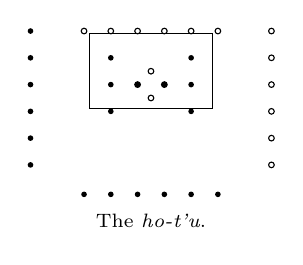
\begin{tikzpicture}[scale=.34,baseline=(current bounding box.center)]
\foreach \y in {0,1,2,3,4,5}{\fill (0,\y) circle (3pt);}
\foreach \x in {2,3,4,5,6,7}{\draw (\x,5) circle (3pt);} 
\draw (2.2,2.1) rectangle (6.8,4.9);
\foreach \x/\y in {3/3,4/3,5/3,6/3,3/4,6/4,3/2,6/2}{\fill (\x,\y) circle (3pt);}
\foreach \x/\y in {4.5/3.5,4.5/2.5,4.0/3.0,5.0/3.0}{\draw (\x,\y) circle (3pt);}
\foreach \y in {0,1,2,3,4,5}{\draw (9,\y) circle (3pt);} 
\foreach \x in {2,3,4,5,6,7}{\fill (\x,-1.1) circle (3pt);} 
\node[font=\scriptsize] at (4.5,-2.1) {The \emph{ho-t'u}.};
\end{tikzpicture}}
\newcommand{\loshudiagram}{%
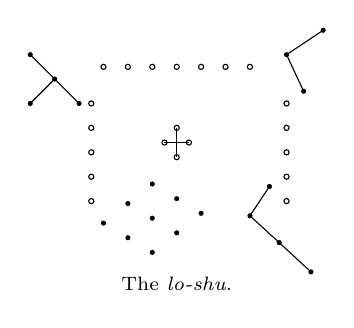
\begin{tikzpicture}[scale=.31,baseline=(current bounding box.center)]
\foreach \p in {(0,6),(1,5),(2,4),(0,4)}{\fill \p circle (3pt);} \draw (0,6)--(1,5)--(2,4); \draw (0,4)--(1,5);
\foreach \x in {3,4,5,6,7,8,9}{\draw (\x,5.5) circle (3pt);} 
\foreach \p in {(10.5,6),(12,7),(11.2,4.5)}{\fill \p circle (3pt);} \draw (10.5,6)--(12,7); \draw (10.5,6)--(11.2,4.5);
\foreach \y in {0,1,2,3,4}{\draw (2.5,\y) circle (3pt);} 
\foreach \p in {(5.5,2.4),(6.5,2.4),(6,1.8),(6,3)}{\draw \p circle (3pt);} \draw (5.5,2.4)--(6.5,2.4); \draw (6,1.8)--(6,3);
\foreach \y in {0,1,2,3,4}{\draw (10.5,\y) circle (3pt);} 
\foreach \p in {(3,-.9),(4,-.1),(5,.7),(4,-1.5),(5,-.7),(6,.1),(5,-2.1),(6,-1.3),(7,-.5)}{\fill \p circle (3pt);} 
\foreach \p in {(9,-.6),(10.2,-1.7),(11.5,-2.9),(9.8,.6)}{\fill \p circle (3pt);} \draw (9,-.6)--(10.2,-1.7)--(11.5,-2.9); \draw (9,-.6)--(9.8,.6);
\node[font=\scriptsize] at (6,-3.4) {The \emph{lo-shu}.};
\end{tikzpicture}}
\newcommand{\magicsquare}{\begin{array}{|c|c|c|}\hline 4&9&2\\\hline 3&5&7\\\hline 8&1&6\\\hline\end{array}}
\newcommand{\tocline}[2]{\noindent\parbox[t]{0.82\linewidth}{#1}\dotfill #2\par}
\newcommand{\toclinewide}[2]{\noindent\parbox[t]{0.86\linewidth}{#1}\dotfill #2\par}
\newcommand{\scandetail}[1]{{\footnotesize\emph{#1}}}
\newcommand{\teubnermark}{%

\begin{tikzpicture}[scale=.42,baseline=(current bounding box.center)]
  \draw[line width=.7pt] (-.55,-.55) rectangle (.55,.55);
  \node[font=\bfseries\Large] at (-.12,.08) {T};
  \node[font=\bfseries\Large] at (.17,-.10) {G};
\end{tikzpicture}}
\newcommand{\bookplateJobAA}{%
\begin{center}
\begin{tikzpicture}[scale=.74]
  \draw[line width=.6pt] (0,0) rectangle (6,8);
  \draw[line width=.35pt] (0.17,0.17) rectangle (5.83,7.83);
  \draw[line width=.35pt] (0.38,0.38) rectangle (5.62,7.62);
  \draw[line width=.35pt] (0.68,1.47) rectangle (5.32,7.37);
  \node[font=\scriptsize] at (1.1,7.05) {ARTES};
  \node[font=\scriptsize] at (3.0,7.18) {1837};
  \node[font=\scriptsize] at (4.9,7.05) {SCIENTIA};
  \node[font=\scriptsize] at (3,6.83) {VERITAS};
  \node[align=center,font=\footnotesize\bfseries] at (3,6.35) {LIBRARY OF THE};
  \node[align=center,font=\small\bfseries] at (3,5.95) {UNIVERSITY OF MICHIGAN};
  \draw (1.12,2.42) rectangle (4.88,5.52);
  \node[align=center,font=\scriptsize] at (3,4.64) {中央印章};
  \node[align=center,font=\scriptsize] at (3,4.30) {TUEBOR};
  \node[align=center,font=\tiny] at (3,3.86) {SI QUAERIS PENINSULAM AMOENAM};
  \node[align=center,font=\tiny] at (3,3.58) {CIRCUMSPICE};
  \draw[line width=.3pt] (1.0,1.82) -- (5.0,1.82);
  \draw (1.0,.56) rectangle (5.0,1.20);
  \node[align=center,font=\scriptsize\bfseries] at (3,.88) {THE GIFT OF\\Prof. ALEXANDER ZIWET};
\end{tikzpicture}
\end{center}}
\newcommand{\dotopen}[2]{\draw (#1,#2) circle (.095);}
\newcommand{\dotfilld}[2]{\fill (#1,#2) circle (.095);}
\newcommand{\hotuJobAA}{%
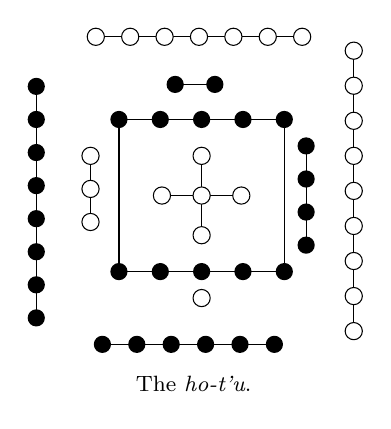
\begin{tikzpicture}[scale=.84,baseline=(current bounding box.center),line cap=round,line join=round]
  \draw[line width=.42pt] (0.00,0.65)--(0.00,4.15);
  \draw[line width=.42pt] (0.90,4.90)--(4.02,4.90);
  \draw[line width=.42pt] (1.00,0.25)--(3.60,0.25);
  \draw[line width=.42pt] (4.80,0.45)--(4.80,4.69);
  \draw[line width=.42pt] (.82,2.10)--(.82,3.10);
  \draw[line width=.42pt] (2.10,4.18)--(2.70,4.18);
  \draw[line width=.42pt] (1.25,1.35) rectangle (3.75,3.65);
  \draw[line width=.42pt] (4.08,1.75)--(4.08,3.25);
  \draw[line width=.42pt] (1.90,2.50)--(3.10,2.50);
  \draw[line width=.42pt] (2.50,1.90)--(2.50,3.10);
  \foreach \y in {0.65,1.15,1.65,2.15,2.65,3.15,3.65,4.15}{\mikafigfill{0.00}{\y}}
  \foreach \x in {1.00,1.52,2.04,2.56,3.08,3.60}{\mikafigfill{\x}{0.25}}
  \foreach \x in {1.25,1.875,2.50,3.125,3.75}{\mikafigfill{\x}{3.65}}
  \foreach \x in {1.25,1.875,2.50,3.125,3.75}{\mikafigfill{\x}{1.35}}
  \foreach \y in {1.75,2.25,2.75,3.25}{\mikafigfill{4.08}{\y}}
  \foreach \x in {2.10,2.70}{\mikafigfill{\x}{4.18}}
  \foreach \x in {0.90,1.42,1.94,2.46,2.98,3.50,4.02}{\mikafigopen{\x}{4.90}}
  \foreach \y in {0.45,0.98,1.51,2.04,2.57,3.10,3.63,4.16,4.69}{\mikafigopen{4.80}{\y}}
  \foreach \y in {2.10,2.60,3.10}{\mikafigopen{.82}{\y}}
  \foreach \x/\y in {1.90/2.50,2.50/2.50,3.10/2.50,2.50/1.90,2.50/3.10,2.50/.95}{\mikafigopen{\x}{\y}}
  \node[font=\footnotesize] at (2.38,-.35) {The \emph{ho-t'u}.};
\end{tikzpicture}}
\newcommand{\loshudiagramJobAA}{%
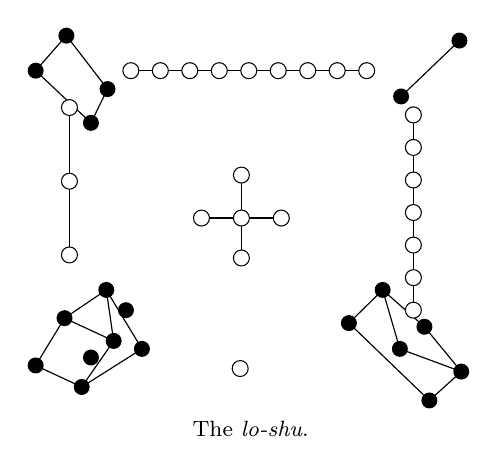
\begin{tikzpicture}[scale=.78,baseline=(current bounding box.center),line cap=round,line join=round]
  \draw[line width=.42pt] (.45,5.35)--(.95,5.92)--(1.62,5.05)--(1.35,4.50)--(.45,5.35);
  \draw[line width=.42pt] (2.00,5.35)--(5.84,5.35);
  \draw[line width=.42pt] (6.40,4.93)--(7.35,5.84);
  \draw[line width=.42pt] (1.00,2.35)--(1.00,4.75);
  \draw[line width=.42pt] (3.15,2.95)--(4.45,2.95);
  \draw[line width=.42pt] (3.80,2.30)--(3.80,3.65);
  \draw[line width=.42pt] (6.60,1.45)--(6.60,4.63);
  \draw[line width=.42pt] (.45,.55)--(1.20,.20)--(2.18,.82)--(1.60,1.78)--(.92,1.32)--(.45,.55);
  \draw[line width=.42pt] (.92,1.32)--(1.72,.95); \draw[line width=.42pt] (1.20,.20)--(1.72,.95)--(1.60,1.78);
  \draw[line width=.42pt] (5.55,1.24)--(6.10,1.78)--(6.78,1.18)--(7.38,.45)--(6.86,-.02)--(5.55,1.24);
  \draw[line width=.42pt] (6.10,1.78)--(6.38,.82)--(7.38,.45);
  \foreach \x/\y in {.45/5.35,.95/5.92,1.62/5.05,1.35/4.50}{\mikafigfill{\x}{\y}}
  \foreach \x/\y in {6.40/4.93,7.35/5.84}{\mikafigfill{\x}{\y}}
  \foreach \x/\y in {.45/.55,.92/1.32,1.20/.20,1.60/1.78,1.72/.95,2.18/.82,1.35/.68,1.92/1.45}{\mikafigfill{\x}{\y}}
  \foreach \x/\y in {5.55/1.24,6.10/1.78,6.38/.82,6.78/1.18,7.38/.45,6.86/-.02}{\mikafigfill{\x}{\y}}
  \foreach \x in {2.00,2.48,2.96,3.44,3.92,4.40,4.88,5.36,5.84}{\mikafigopen{\x}{5.35}}
  \foreach \y in {2.35,3.55,4.75}{\mikafigopen{1.00}{\y}}
  \foreach \x/\y in {3.15/2.95,3.80/2.95,4.45/2.95,3.80/2.30,3.80/3.65}{\mikafigopen{\x}{\y}}
  \foreach \y in {1.45,1.98,2.51,3.04,3.57,4.10,4.63}{\mikafigopen{6.60}{\y}}
  \mikafigopen{3.78}{.50}
  \node[font=\footnotesize] at (3.95,-.48) {The \emph{lo-shu}.};
\end{tikzpicture}}
\newcommand{\gridsquarebase}{\draw[step=1] (0,0) grid (7,7);}
\newcommand{\diagonsquare}{%
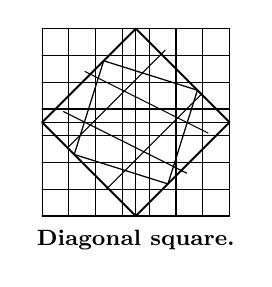
\begin{tikzpicture}[scale=.34,baseline=(current bounding box.center),line cap=round,line join=round]
  \gridsquarebase
  \draw[line width=.7pt] (3.5,7)--(7,3.5)--(3.5,0)--(0,3.5)--cycle;
  \draw[line width=.45pt] (2.3,5.8)--(5.8,4.7)--(4.7,1.2)--(1.2,2.3)--cycle;
  \draw (.8,3.9)--(5.4,1.6); \draw (1.6,5.4)--(6.2,3.1); \draw (1.0,2.6)--(4.6,6.2); \draw (2.4,1.0)--(6.0,4.6);
  \draw (3.5,0)--(3.5,7); \draw (0,3.5)--(7,3.5);
  \node[font=\footnotesize\bfseries] at (3.5,-.9) {Diagonal square.};
\end{tikzpicture}}
\newcommand{\breadthsquare}{%
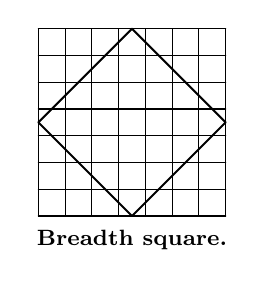
\begin{tikzpicture}[scale=.34,baseline=(current bounding box.center),line cap=round,line join=round]
  \gridsquarebase
  \draw[line width=.7pt] (3.5,7)--(7,3.5)--(3.5,0)--(0,3.5)--cycle;
  \draw[line width=.55pt] (3.5,7)--(7,3.5); \draw[line width=.55pt] (0,3.5)--(3.5,7);
  \node[font=\footnotesize\bfseries] at (3.5,-.9) {Breadth square.};
\end{tikzpicture}}
\newcommand{\lengthsquare}{%
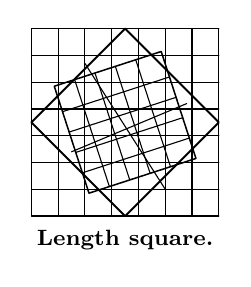
\begin{tikzpicture}[scale=.34,baseline=(current bounding box.center),line cap=round,line join=round]
  \gridsquarebase
  \draw[line width=.7pt] (3.5,7)--(7,3.5)--(3.5,0)--(0,3.5)--cycle;
  \begin{scope}[rotate around={18:(3.5,3.5)}]
    \draw[line width=.55pt] (1.4,1.4) rectangle (5.6,5.6);
    \foreach \x in {2.2,3.0,3.8,4.6}{\draw (\x,1.4)--(\x,5.6);} 
    \foreach \y in {2.2,3.0,3.8,4.6}{\draw (1.4,\y)--(5.6,\y);} 
  \end{scope}
  \draw (1.5,2.4)--(5.8,4.2); \draw (2.0,5.7)--(5.0,1.0);
  \node[font=\footnotesize\bfseries] at (3.5,-.9) {Length square.};
\end{tikzpicture}}
\newcommand{\fangtableA}{\begin{tabular}{|c|c|c|l|}\hline 1&2&3&1st class\\\hline 2&3&2&2nd ``\\\hline 3&1&1&3rd ``\\\hline 26&34&39&measures\\\hline\end{tabular}}
\newcommand{\fangtableB}{\begin{tabular}{|c|c|c|l|}\hline 1&0&3&1st class\\\hline 2&5&2&2nd ``\\\hline 3&1&1&3rd ``\\\hline 26&24&39&measures\\\hline\end{tabular}}
\newcommand{\fangtableC}{\begin{tabular}{|c|c|c|l|}\hline 0&0&3&1st class\\\hline 4&5&2&2nd ``\\\hline 8&1&1&3rd ``\\\hline 39&24&39&measures\\\hline\end{tabular}}
\newcommand{\fangtableD}{\begin{tabular}{|c|l|}\hline 36&third class\\\hline 99&measures\\\hline\end{tabular}}
\newcommand{\fangtableE}{\begin{tabular}{|c|c|c|l|}\hline 1&&2&1st class\\\hline &3&1&2nd ``\\\hline 4&1&&3rd ``\\\hline 1&1&1&measures\\\hline\end{tabular}}
\newcommand{\fangtableF}{\begin{tabular}{|c|c|c|l|}\hline $-5$&3&2&cows\\\hline 6&$-9$&5&sheep\\\hline 8&3&$-13$&hogs\\\hline $-600$&&1000&pieces\\\hline\end{tabular}}
\newcommand{\mikafigopen}[2]{\path[fill=white] (#1,#2) circle (.13);\draw[line width=.38pt] (#1,#2) circle (.13);}
\newcommand{\mikafigfill}[2]{\fill (#1,#2) circle (.13);}
\newcommand{\rodglyph}[2]{\raisebox{-0.25ex}{\includegraphics[height=#1,keepaspectratio]{#2}}}
\newcommand{\sourceasset}[2]{\begin{center}\includegraphics[width=#1,keepaspectratio]{#2}\end{center}}
\newcommand{\tg}{\mathop{\mathrm{tg}}}
\newcommand{\arcop}{\mathop{\mathrm{arc}}}
\newcommand{\versin}{\mathop{\mathrm{versin}}}
\newcommand{\rectsym}{\mathord{\raisebox{0.15ex}{\begingroup\setlength{\fboxsep}{0pt}\setlength{\fboxrule}{0.35pt}\fbox{\rule{0pt}{0.55ex}\rule{0.9ex}{0pt}}\endgroup}}}
\newcommand{\sourceassetJobAJ}[2][width=.84\linewidth]{\begin{center}\includegraphics[#1]{#2}\end{center}}
\newcommand{\dd}{\mathbin{\cdot}}
\begin{document}
\begin{titlepage}\centering
{\Large 三上義夫}\par\vspace{1em}
{\Huge 中国および日本における\\[0.3em]数学の発展}\par\vspace{0.6em}
{\large Yoshio Mikami, \emph{The Development of Mathematics in China and Japan}}\par\vspace{1.5em}
{\large ライプツィヒ：B.\ G.\ トイプナー、1913年}\par
{\large 『数学的諸科学の歴史論集』第30冊}\par\vfill
{\normalsize 日本語訳（全366 PDF頁、図版は原本スキャンより）。AIによる翻訳。巻末の編集注を参照。}\par
\end{titlepage}
\tableofcontents
% PDF page 1: cover, no printed text.
% PDF page 2: bookplate, no printed text.
% PDF page 3: call-number endpaper, no printed text.
% PDF page 4: blank endpaper, no printed text.
\scanpage{0005}{標題紙}
\begin{center}
数学諸科学史ならびにその応用を含む論叢\\
モーリッツ・カントール創刊。第XXX冊。

\par\vspace{.35em}
\rule{\linewidth}{0.45pt}\\[-.35em]
\rule{\linewidth}{0.2pt}

\vspace{4em}
{\LARGE 中国および日本における\\ 数学の発展}

\vspace{2em}
著者

\vspace{1em}
{\large 三上義夫}\\[-.15em]
\rule{1.25em}{0.35pt}\\[-.42em]
\rule{.85em}{0.2pt}

\vspace{4em}
本文中に67図を含む

\vspace{3em}

\includegraphics[width=1.15cm]{pdf005-teubner-monogram.png}

\vspace{6em}
\begin{tabular}{ccc}
\underline{ニューヨーク} & ライプツィヒ：B. G. TEUBNER & \underline{ロンドン}\\
G. E. STECHERT \& Co. & POSTSTRASSE 3 & WILLIAMS \& NORGATE\\
151--155 WEST 25th ST. & 1913 & 14 HENRIETTA STREET\\
& & COVENT GARDEN W. C.
\end{tabular}
\end{center}
\scanfooter

\scanpage{0006}{著作権頁}
\begin{center}
\vfill
無断転載を禁ず\\
B. G. TEUBNER（ドレスデン）印刷
\end{center}
\scanfooter

\scanpage{0007}{献辞}
\begin{center}
著者は本書を\\[.5em]
恩人たちに献呈する\\[1.2em]
{\large 男爵 D. KIKUCHI}\\[.5em]
N. OKAMOTO 氏\\[.5em]
および\\[.5em]
{\large T. ENDŌ 氏}
\end{center}
\scanfooter

% PDF page 8: blank verso, no printed text.

\scanpage{0009}{ジョージ・ブルース・ハルステッドによる序文}
\begin{center}{\Large 序文}\end{center}

英語がすでに世界語であることについて、中国数学史が日本で書かれ、アメリカで改訂され、ヨーロッパで出版されるという事実以上に鮮やかな証拠があり得るだろうか。しかし当然ながら、これは英国の慣用語でも合衆国の慣用語でもないし、私もそれをそのように狭めようとはしなかった。本書との私自身のわずかな関係は、日本が非ユークリッド幾何の重要性を最初に認めた国であったことに由来する。当時日本で利用可能であったのは私の『ボーヤイ』と『ロバチェフスキー』だけであり、それが東京で私の二つの小著を再刊するに至った。各巻には、文部大臣であり現在は京都大学総長である菊池男爵による序文が付された（一つ目の日付は1892年2月15日）。日本人の眠っていた幾何学的天才がその後どれほど驚くべき仕方で目覚めたかを知るには、本書の著者が編んだ『極東からの数学論文』（Teubner, 1910）を参照されたい。そこでは55篇の論文（1892年から1907年まで）のうち24篇が幾何学に属している。

本史書の著者が旧日本の偉大な数学巨人の最後の一人を個人的に知っていたことは、ロマンティックな幸運である。

\begin{flushleft}グリーリー、コロラド、U. S. A.\end{flushleft}
\begin{flushright}George Bruce Halsted.\end{flushright}
\scanfooter

\scanpage{0010}{緒言、第1頁}
\begin{center}{\Large 緒言}\end{center}

中国および日本において発展した数学についての歴史的記述は、さまざまな著者によってなされてきた。しかしそれらはすべて各種の雑誌に散在しており、われわれは容易に接することができない。この主題に特に捧げられて、単独の著作として刊行されたものをわれわれは知らない。なるほど、中国の阮元の『数学者・天文学者伝』のように、18世紀末に現れた書物、また遠藤利貞の『大日本数学史』（東京、1896年）のような書物は存在する。これらはたしかに貴重な情報源であるが、中国語または日本語で書かれているため、ヨーロッパおよびアメリカの読者にはほとんど役立たない。そこでわれわれは本巻を編むことにした。西洋の読者にこの主題についていくらかの知識を与えることができれば、われわれは十分満足するであろう。

私の研究成果は、歴史としては決して完全ではない。そのため私はこの表題を避けた。私の叙述はむしろ歴史資料の集成である。しかもそのようなものとしてさえ、あまりにも貧弱で不十分である。読者にはあらかじめ、日本および中国の旧数学者たちが扱った他の多くの主題がまだ存在し、本書ではそれらに触れていないことを告げておかなければならない。

日本数学については、私は現在ニューヨークの D. E. Smith 博士とともに、通俗的に書かれた著作を共同で執筆している。その歴史は非常に簡略ではあるが、この主題について良い概観を与えるであろう。そこに扱われる日本人精神の産物の一部は、本巻には再録されていない。そこでわれわれは、日本数学については総説と年表を与え、その後にいくつかの特定主題を記すことにした。これが、日本数学と中国の学問とについて叙述の方針を異ならせた理由である。

本巻全体を通じて、私は他国民の数学的業績との比較をほとんど、またはまったく行っていない。数学的観念がどのような発展過程を通じて生じたかについても、特には説明していない。もっともその方向の研究こそ私の理想である。これらはすべて、さらに成熟した研究に委ねられる。

古い数学書は、写本であれ版本であれ、いまや収集が非常に困難である。そのため私は資料を得るにあたって少なからぬ困難を経験した。
\scanfooter

\scanpage{0011}{緒言、第2頁}
しかしそれにもかかわらず、友人たちが示してくれた厚意と同情に対して、私はきわめて深く感謝しなければならない。そのおかげで、若干の些細な部分を除き、主として原資料にもとづいて研究を進めることができたからである。本書を完成するにあたり、これらの諸氏の助力に対する私の負債を認めなければならない。とりわけ T. Endō 氏、Y. Fujikawa 博士、故 T. Hagiwara 氏、G. B. Halsted 教授、T. Hayashi 教授、K. Kano 博士、C. Kawakita 氏、D. Kikuchi 男爵、S. Mikami 教授、N. Okamoto 氏、K. Uyeno 氏に感謝する。

\begin{center}\rule{3cm}{0.4pt}\end{center}

中国の表意文字の読みは、すべて現在一般に行われている方法に従った。中国では同じ表意文字すなわち字が古代から今日まで用いられてきたが、その読みは変化を経ている。日本で用いられる表意文字は、ほとんどすべて中国からもたらされたものであるが、日本での読み方は中国の読み方とはまったく異なり、むしろ中国で古く行われた一体系に似ていると言われる。しかし中国の表意文字の読み方の変化は、一般に東洋学者によって無視されてきたので、われわれもその慣用に従った。また、諸時代・諸地方における正確な読みを跡づけることも容易ではない。今日でさえ、表意文字は必ずしも一義的に読まれるわけではなく、地方によって読みが異なることもある。したがって、同一人物の名がヨーロッパおよびアメリカの東洋学者の著述において四通り、五通りに綴られることも少なくない。ゆえに読者には、本書に示した中国名の綴りにあまり大きな重要性を置かないようお願いしなければならない。

中国人名では、姓を先に書き、それに個人名を続ける。この点で中国名は西洋名と異なる。

日本でも、中国と同様、姓を先に書く。

日本語では、ただ一つ \emph{n} で終わる場合を除き、すべての音節が母音で終わる。\emph{n} の音が \emph{b}、\emph{p}、または \emph{m} の前に来るとき、それは \emph{m} に変わり、日本人の欧文筆者は通常そのように綴る。便宜のため、われわれも \emph{kitto} や \emph{itchi} のような綴りを用いる。母音 \emph{a}, \emph{i}, \emph{u}, \emph{e}, \emph{o} はドイツ語の短音にいくらか似て発音すべきで、その音はすべて非常に短い。\emph{o} と \emph{u} の長音は \emph{ō} と \emph{ū} で表し、その長さを除けば短音と同じ性質のものである。\emph{Ai}, \emph{ei}, \emph{ii} などは、二つの母音の音をともに発音して読むべきである。\emph{Ku} はほとんど \emph{k} のように発音すべきである。正しくは \emph{ku} を含む語が、時に \emph{k} の字だけで示されたこともある。

日本の固有名の正しい読みを知ることは、時に非常に困難である。たとえば一人の数学者の名は
\scanfooter

\scanpage{0012}{緒言、第3頁}
R. Fujisawa によって Yasushima と読まれ、D. Kikuchi によって Ajima と読まれた。しかし姓は比較的読みやすい。個人名ははるかに難しい。そのためわれわれは、真の読み方に関係なく、表意文字自体の音に従う一般的な読み方でそのような名を読むことに慣れている。われわれは Seki Kōwa と読むが、彼の個人名 Kōwa は Takakazu と読まれるべきであった。Takahashi Shiji の個人名は T. Hayashi により Shigetoki または Yoshitoki と読まれたが、他の者は Munetoki と読んだ。しかし実際には、われわれはその名の真の読みについて何も知らないので、表意文字の一般的な読み方に従って Shiji と読むほかない。私と Hayashi との読みの相違（彼の『日本数学小史』、\emph{Nieuw Archief voor Wiskunde} 所収）は、ほとんどこのようにして生じた。

天文学者 Yamaji Shūjū の子孫はすぐれた歴史家・思想家であるが、彼自身が私に語ったところでは、Shūjū という名をどう読むべきかを彼は知らない。Saitō Gigi は T. Hagiwara の師であったが、後者は私に、師の個人名 Gigi の真の読みを学んだことがないと語った。古い日本人の個人名は、たとえば書物に署名するような、重大または厳粛な場合にだけ用いられた。日常の場合には、これらの名は用いられず、各人は通称を持っていた。Seki の通称は Shinsuke であり、そのため彼は時に Seki Shinsuke と呼ばれる。

古い日本の写本は、さまざまな誤りを免れない。著者自身の自筆稿でさえそうである。幾人もの写字生の手を経た写本では、誤りはとくに多い。われわれが参照に用いたものも、これらの欠点を免れていない。同一写本のさまざまな写しを比較すると、部分によって互いにかなり異なるところが見つかることがある。しかしこれらの写本に犯された誤りは一般に容易には発見できないので、私の叙述においてそれらの誤りが必ずしもすべて訂正されているわけではない。もっとも、このような事情を考慮に入れる読者が、本書に気づかれずに残っている欠点について、われわれをあまり咎めないことを望む。

\begin{flushleft}上総大原、1910年9月20日。\end{flushleft}
\begin{flushright}Y. Mikami.\end{flushright}
\scanfooter


\scanpage{0013}{目次、第1頁}
\begin{center}{\Large 目次}\end{center}
\begin{flushright}{\footnotesize Page}\end{flushright}
\begingroup\small\setlength{\parskip}{0.18em}
\tocline{序文。G. B. Halsted 教授による}{V}
\tocline{緒言}{VI}
\tocline{目次}{IX}
\tocline{\textbf{第一部 中国数学}}{1}
\tocline{\quad 第1章 中国数学の最古期}{1}
\tocline{\quad 第2章 周髀（Chou-Pei）}{4}
\tocline{\quad 第3章 九章算術（Chiu-chang Suan-shu）}{8}
\tocline{\quad 第4章 孫子算経、または Sun-Tsŭ の算術古典}{25}
\tocline{\quad 第5章 海島算経、または海島算術古典}{33}
\tocline{\quad 第6章 五曹算経ならびに Hsia-hou Yang、Chang Ch'iu-chien、\\\hspace*{2.8em}Chen Luan の著作}{37}
\tocline{\quad 第7章 古い中国数学者による円測}{46}
\tocline{\quad 第8章 Wang Hsiao-t'ung と三次方程式}{53}
\tocline{\quad 第9章 インドの影響について}{56}
\tocline{\quad 第10章 Ch'ên Huo}{61}
\tocline{\quad 第11章 Ch'in Chiu-shao}{63}
\tocline{\quad 第12章 Li Yeh}{79}
\tocline{\quad 第13章 Yang Hui}{84}
\tocline{\quad 第14章 Chu Shih-chieh}{89}
\tocline{\quad 第15章 アラビアの影響および Kuo Shou-ching}{98}
\tocline{\quad 第16章 明代の数学}{108}
\tocline{\quad 第17章 ヨーロッパ数学の導入}{112}
\tocline{\quad 第18章 古い数学様式の復興とその後の時代の状態}{120}
\tocline{\quad 第19章 方程式解法の後代における進展}{128}
\tocline{\quad 第20章 後代中国数学者による $\pi$ の値の研究}{135}
\tocline{\quad 第21章 円測に関する解析的研究。無限級数}{142}
\tocline{\textbf{第二部 日本数学}}{156}
\tocline{\quad 第22章 日本数学の概観}{156}
\tocline{\quad 第23章 日本数学の年表}{178}
\tocline{\quad 第24章 関の行列式概念}{191}
\tocline{\quad 第25章 日本数学者が用いた $\pi$ の値}{200}
\tocline{\quad 第26章 日本数学者による球体積の研究}{203}
\tocline{\quad 第27章 日本数学者による球面積求法の研究}{206}
\endgroup
\scanfooter

\scanpage{0014}{目次、第2頁}
\begin{flushright}{\footnotesize Page}\end{flushright}
\begingroup\small\setlength{\parskip}{0.18em}
\tocline{\quad 第28章 1709年『括要算法』における円弧の平方の公式}{210}
\tocline{\quad 第29章 日本数学者が用いた $\pi$ のいくつかの級数}{213}
\tocline{\quad 第30章 久留島の円測}{217}
\tocline{\quad 第31章 久留島による二次無理数の連分数法}{223}
\tocline{\quad 第32章 松永写本における不定解析の問題}{229}
\tocline{\quad 第33章 不定方程式 $x^p-ky=a$}{237}
\tocline{\quad 第34章 阿島の Renjutsu Henkan}{238}
\tocline{\quad 第35章 円内に連続して内接する円が冠をなす場合についての\\\hspace*{2.8em}阿島の研究}{243}
\tocline{\quad 第36章 不定方程式 $x_1^2+x_2^2+x_3^2+x_4^2+x_5^2=y^2$ の会田の解法}{247}
\tocline{\quad 第37章 会田の楕円研究}{249}
\tocline{\quad 第38章 白石による楕円体面の計算}{256}
\tocline{\quad 第39章 坂部・川井の方程式解法}{260}
\tocline{\quad 第40章 y\,e\,n\,r\,i 計算に用いられた若干の表と無限次方程式}{268}
\tocline{\quad 第41章 Hasegawa の Kyūseki Tsūkō における楔形断面について}{284}
\tocline{\quad 第42章 魔方陣}{290}
\tocline{\quad 第43章 懸垂線}{294}
\tocline{\quad 第44章 Hagiwara Teisuke}{301}
\tocline{\quad 第45章 平面上に立つ環のまわりを球が転がるときに描く曲線の\\\hspace*{2.8em}面積についての萩原の公式}{311}
\tocline{\quad 第46章 斜曲面}{315}
\tocline{\quad 第47章 日本数学史研究についての短い記述}{322}
\tocline{索引}{331}
\endgroup
\scanfooter

\scanpage{0015}{第一部・第1章、第1頁}
\begin{center}
第一部\\[1em]
{\Large 中国数学}\\[1em]
第1章\\
{\large 中国数学の最古期}
\end{center}
\phantomsection\addcontentsline{toc}{section}{第I部　中国の数学}
\phantomsection\addcontentsline{toc}{subsection}{第1章　中国数学の最古期}

中国は世界でもっとも古い国民の一つである。古さにおいて中国はエジプトおよびバビロンとだけ比較され得るのであり、他のどの国とも比較できない。中国史のより遠い時代へどれほど遡って探究しても、われわれはそこに初期文化の痕跡をいくらか見出す。土着の年代記によれば、中国人は過去数万年にわたって文明を享受してきた。文明生活の早い勃興とともに、数学もまた疑いなく早い時代に萌した。中国人は最古の時代から、宗教儀礼に非常に注意深く、暦法の規定に最大限の配慮を払う民族であった。したがって古代においてさえ、算術的技芸が慎重に培われていたことにはまったく疑いがない。しかし、遠い古代におけるこの学問の成長を調べようとするとき、古い文献や記録がまったく欠けているため、われわれはまったく途方に暮れる。

中国が古い国民であることには疑いがない。しかし中国人は、黄河と揚子江に潤された広大な土地に常に住んでいたわけではない。彼らは西方から来て、現在住んでいるところに定着したのである。彼らは時にバビロニア人と同族に近い種族であると言われる。若干の学者が指摘するように、極めて古い時代における両民族の文明は、かなりの程度で互いに似ている。もしそうならば、中国人が古代において、西方の同胞が持っていたのと同じ算術規則の知識を有していた可能性はないだろうか。しかし現在のところ、われわれはこの見解を肯定することも否定することもできない。したがって少なくともここでは、中国で発展した数学とバビロニア人によって培われた数学との相互関係について論じないことにする。よってこの

\scanfooter

\scanpage{0016}{第一部・第1章、第2頁}
\setcounter{footnote}{0}
興味深い問題は、今後の研究成果に委ねて手を付けないまま残さなければならない。

古い文献によれば、黄帝すなわち Yellow Emperor は、I-hai に太陽を占わせ、Chang-i に月を占わせ、Yü-ch’ü に星を占わせ、Ling-lun に楽律を定めさせ、Tai-nao に \emph{chia-tsŭ} すなわち干支的な六十進体系を作らせ、Li-shou に数または数の術を発明させ、Yung-ch’éng にこれら六つの術をすべて用いて暦を定めさせた。\footnote{Yüan Yüan, \emph{Ch’ou-jen Ch’uan} すなわち “Biographical Collections of Astronomers and Mathematicians”, Book 1.} よく知られているように、黄帝は紀元前27世紀に中国を治めた。

黄帝の時代から今日まで常に用いられてきた \emph{chia-tsŭ} は、二つの体系を対応させることから成っている。その二体系とは、\emph{chia}, \emph{i}, \emph{ping}, \emph{hsü}, \emph{chi}, \emph{kong}, \emph{hsin}, \emph{jen}, \emph{kuei} と、\emph{tsŭ}, \emph{ch’ou}, \emph{yin}, \emph{mao}, \emph{ch’én}, \emph{szŭ}, \emph{wu}, \emph{wei}, \emph{shen}, \emph{yu}, \emph{wu}, \emph{hai} である。

\emph{chia-tsŭ} の列挙体系では、第一、第二、以下は \emph{chia-tsŭ}, \emph{i-ch’ou}, \ldots\ と表される。わかりやすくするために、10周期と12周期の各成分をそれぞれ $A_1,A_2,\ldots,A_{10}$ および $B_1,B_2,\ldots,B_{12}$ と表すならば、列挙は下のように進む。
\[
\begin{aligned}
A_1B_1&=1,\quad A_2B_2=2,\ldots, A_{10}B_{10}=10,\\
A_1B_{11}&=11,\quad A_2B_{12}=12,\quad A_3B_1=13,\ldots, A_{10}B_8=20,\\
A_1B_9&=21,\ldots, A_4B_{12}=24,\quad A_5B_1=25,\quad A_6B_2=26,\\[-.5em]
&\hspace{4em}\cdots\cdots\cdots\cdots\cdots\\[-.5em]
A_{10}B_2&=50,\quad A_1B_3=51,\ldots, A_9B_{11}=59,\quad A_{10}B_{12}=60.
\end{aligned}
\]
60を超えると、同じ列挙が再び反復周期として戻る。年と日はこの方式で番号づけられてきた。方位もまた、全円周を60部分に分けるこの方式によって示された。

Li-shou は、算術書 \emph{Chiu-chang} すなわち「九章」の著者として言及されることがあり、そこから現存する \emph{Chiu-chang Suan-shu} すなわち『九章算術』が度重なる改訂によって生じたとされる。しかしこの見解はおそらく作り話に過ぎない。宋代の末ごろには、たしかに \emph{Huang-Ti Chiu-chang} すなわち『黄帝九章』という題名の書物があったが、それは後代の学者による単なる創作らしい。Li-shou がこれほど早い時代に確立した算術がどのような種類のものであったかを知る手段はない。
\scanfooter

\scanpage{0017}{第一部・第1章、第3頁}
\setcounter{footnote}{0}
3500年以上前のことである。われわれは、そのような大古に発展した学問は必然的にごく初歩的なものであったに違いない、と合理的に推測できるだけである。『九章算術』に示されているように高度に発達した体系が、黄帝の時代に存在し得たとは、われわれは信じない。この書の内容については、それに特に割いた章で記述を試みるつもりである。

聖典 \emph{I-ching} の \emph{Hsi-tzŭ} の章には、河が \emph{t’u} を作り、洛が \emph{shu} を作った、と記されている。これは、\emph{ho-t’u} と \emph{lo-shu} と呼ばれる図が占いに用いられたことを意味する。伝承によれば、前者は紀元前29世紀の伏羲帝の時代から伝わる。その時、竜馬が河に現れ、その足跡が \emph{pa-kua} の図を残し、これは占断に役立ってきた。\emph{lo-shu} は、賢人禹の時代からわれわれに伝わる。禹は偉大な政治家であり啓明的な帝王であった。彼が災厄をもたらす氾濫しつづける黄河に堤を築いていたとき、神聖な亀が現れ、その背は1から9までの数で作られた図によって飾られていた。この偉大な賢人はそれを記録し、応用した。\emph{ho-t’u} と \emph{lo-shu} は、中国の書物では下に示すように現れる。

\begin{center}
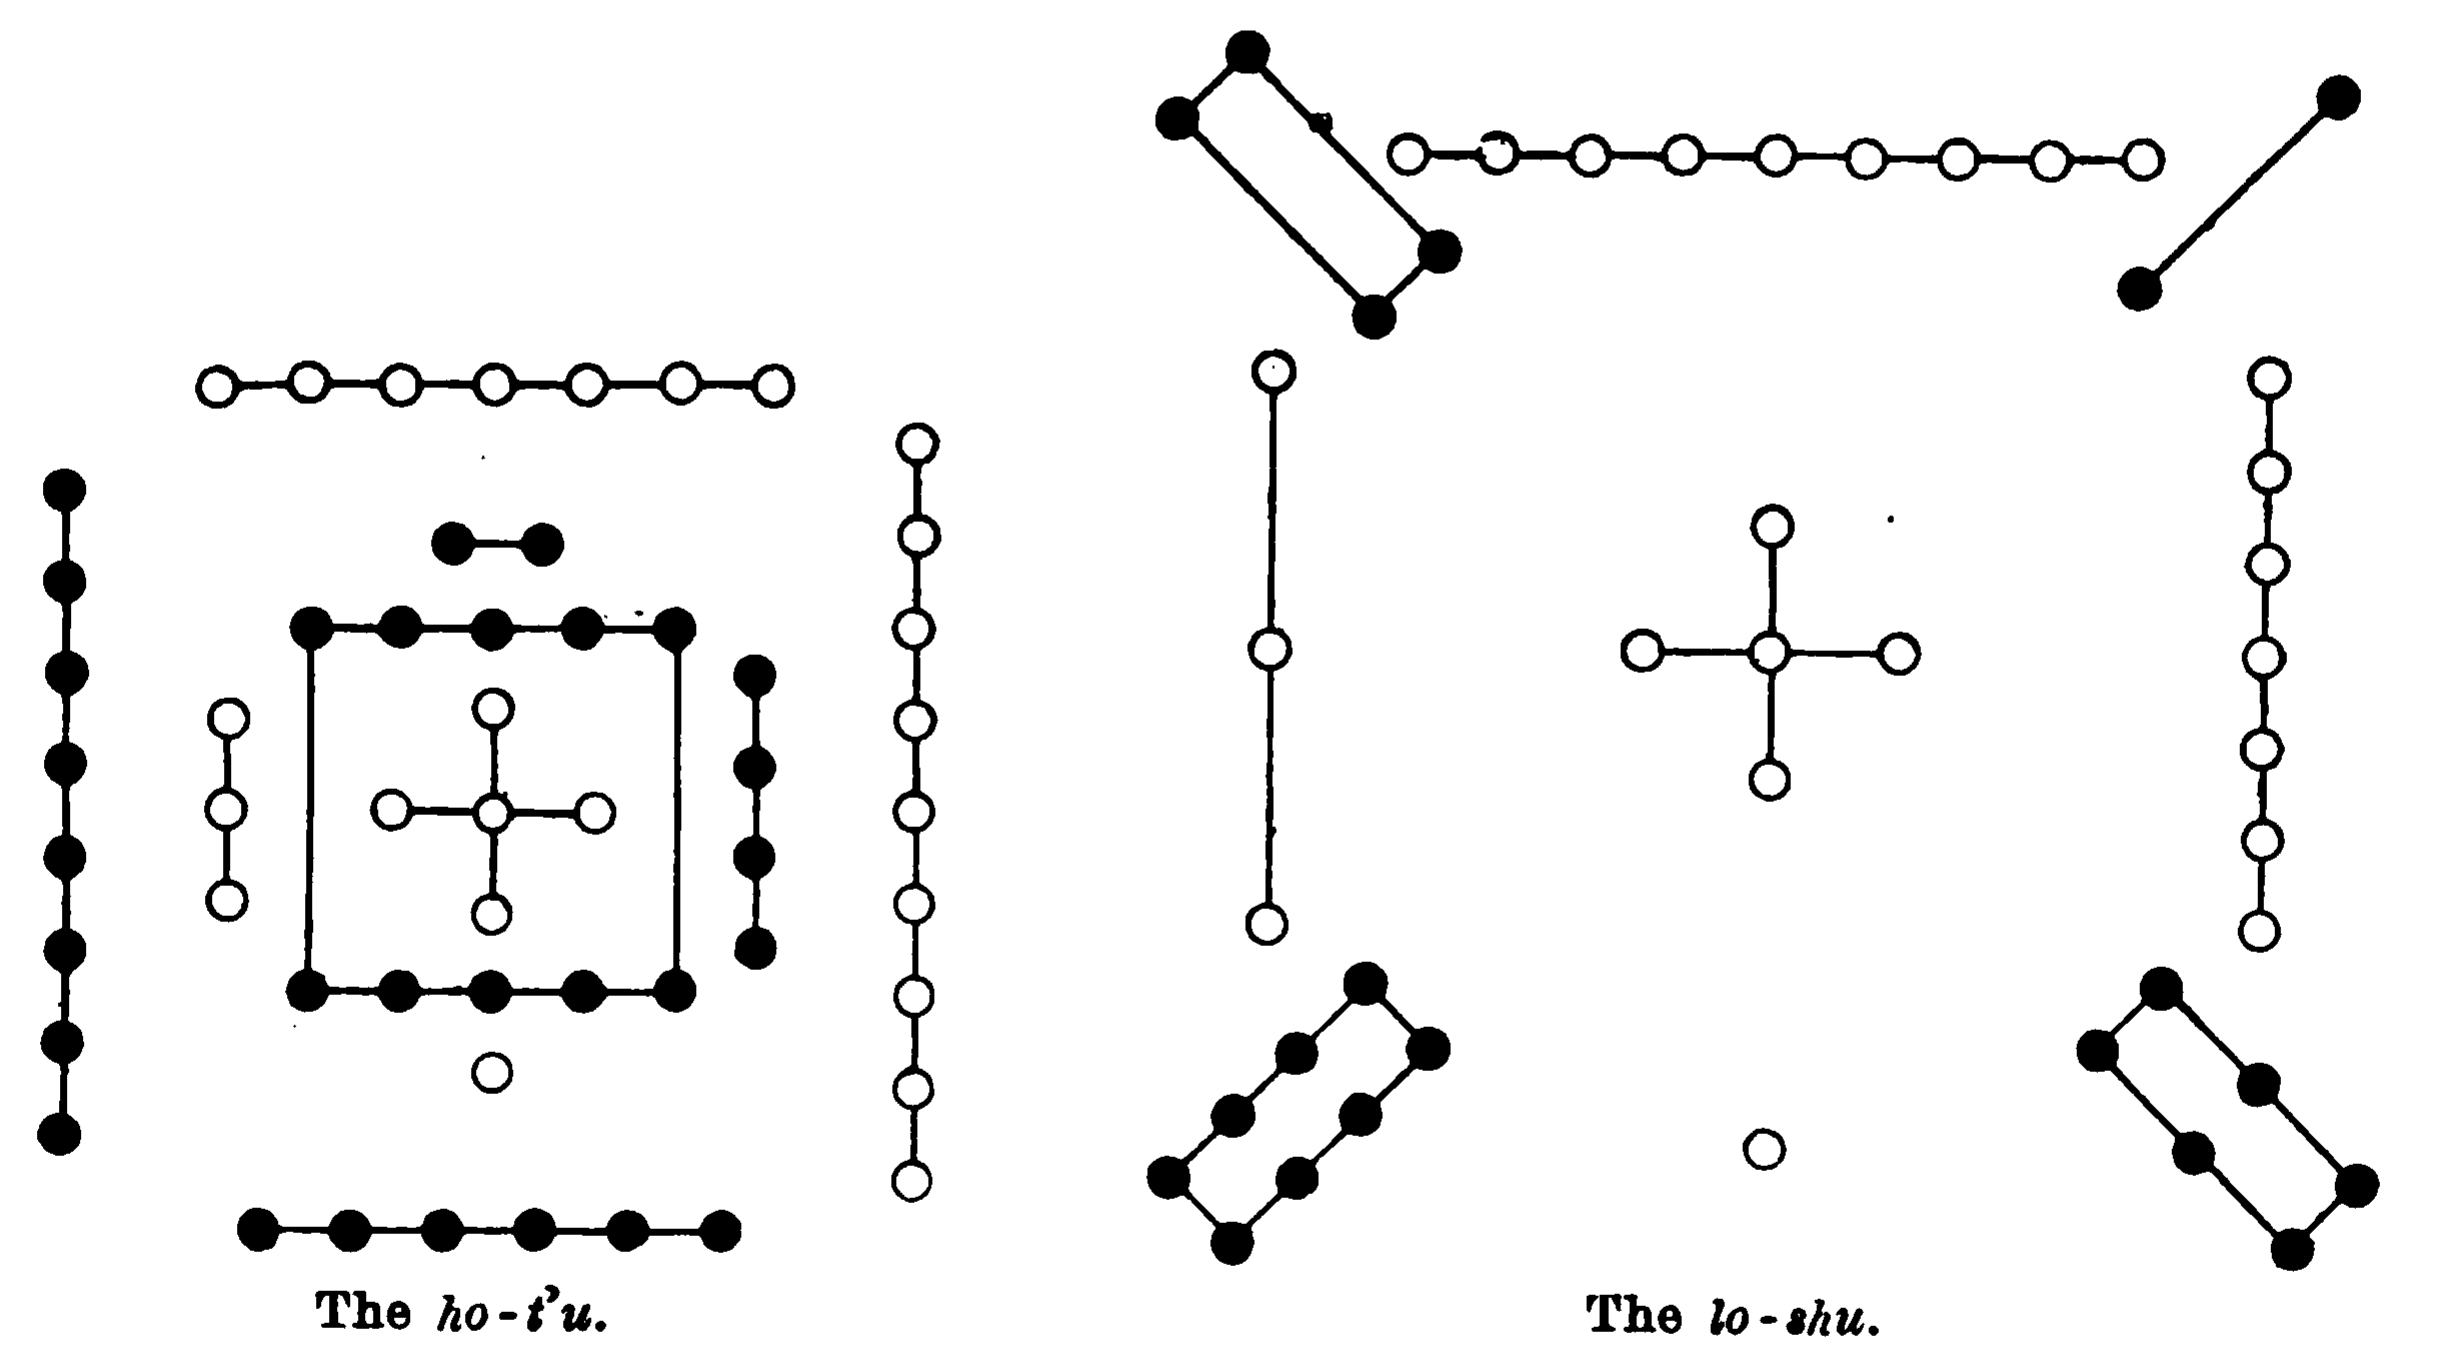
\includegraphics[width=.92\linewidth]{pdf017-hotu-loshu.png}
\end{center}

\emph{lo-shu} は、九つの数字を要素とする魔方陣であり、添えた図の通りである。したがって後代の中国では、また若干の初期日本数学者によっても、魔方陣はこの名で呼ばれるようになった。\footnote{中国語の \emph{lo-shu} は日本では \emph{rakusho} と読まれた。}
\begin{center}
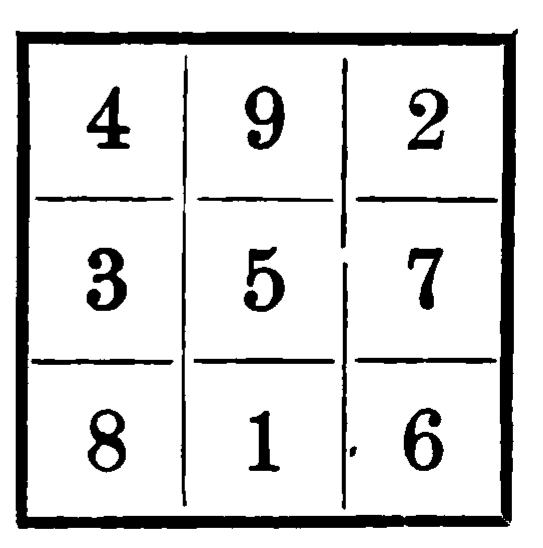
\includegraphics[width=.20\linewidth]{pdf017-magic-square.png}
\end{center}
\scanfooter

\scanpage{0018}{第一部・第二章、印刷頁4}
\begin{center}
CHAPTER 2.\quad THE CHOU-PEI.\\
第二章　周髀。
\phantomsection\addcontentsline{toc}{subsection}{第2章　周髀}
\end{center}

今日まで伝存する古代中国人の残した最古の数学的著作は、疑いなく『\emph{Chou-pei}』、すなわち『\emph{Chou-pei Suan-ching}』である。語 \emph{suan-ching} は字義どおりには「数学の経典」または「算術の聖典」と訳すべきものである。しかし厳密にいうと、『\emph{Chou-pei}』は数学書ではなく、暦法上の主題を扱う書である。それでも、中国数学史においてはこの上なく重要な関心をもつものである。

『\emph{Chou-pei}』の著者はつねに不明のままであり、それがいつ作られたかも知られていない。また、この書全体が一時に作られたのか、いくつかの異なる時期に作られたのかも疑わしい。われわれに伝えられた『\emph{Chou-pei}』は二巻から成り、その第二巻はこの場ではほとんど関係のない暦法理論を扱っている。『\emph{Chou-pei}』第一巻には、賢王 Chou-Kong とその学識ある大臣 Shang Kao との間に交わされた有名な対話が記されている。この対話に続いて、Ying Fang と Ch'ên-Tsŭ との別の対話が置かれている。これらの人物がどの時代に生きたかは知られていない。一般に信じられている、むしろ想像されているところでは、この第二の対話は後代の筆者による補入であるらしい。第二の対話の次にはさらに、Lü-Shih、すなわち紀元前三世紀に Ch'in 王朝の有力な大臣であった Lü Pu-i が書いた、または教えたものとして記録された一節がある。いずれにしても、この第二の対話に登場する人物たちは、Chou 王朝末期またはそれ以前に生きていたに違いない。

『\emph{Chou-pei}』は、Chang Chun-ch'ing、Ch'ên Luan、Li Ch'un-fêng その他の注釈によって保存されてきた。これら注釈者のうち最初の人物の年代は、後代の中国の著述家によって不明とされている。しかしその序は、Chang Hêng によって作られた天文学書 \emph{Ling-hsien} に言及している。このことは、Chang Hêng が一三九年に没しているので、Chang Chun-ch'ing が紀元二世紀またはそれ以後に生きたことをよく示している。

『\emph{Chou-pei}』、少なくともその増補部分の成立は比較的新しい時代のものかもしれないが、そこに記録された対話は、中国人が紀元前十二世紀という早い時代に到達していた数学的研究の状態をわれわれに示してくれる。というのは、Chou-Kong が没したのは一一〇五年であったからである。Chou-Kong は Chou 王朝の王 Wu-Wang の弟であり、
\scanfooter

\scanpage{0019}{第二章、印刷頁5}
その幼い甥 Ch'êng-Wang が王位に就いていたとき、中国を摂政として治めた。

その対話は次のように進む。

「昔、Chou-Kong は Shang Kao に尋ねた。私は、あなたが数の術に通じていると聞いているので、あなたに問いたい。昔 Fu-hi は天を測り暦を定めた。しかし天は登ることのできるものではなく、地はわれわれの尺度によって測定できるものでもない。それならば、天と地の数は何によって導かれるのか。

「Shang Kao は答えた。数の術は円と方から導かれる。円は方から導かれ、方は \emph{kuei}、すなわち直角の線尺から導かれる。線尺は 9 を 9 に入れることから来て、これは 81 を作る。そこで線尺を分け、\emph{kou} すなわち幅を 3、\emph{ku} すなわち長さを 4 とすれば、角を結ぶ距離は 5 である。外の数の平方を取り、半分にすると、線尺が得られる。」

この最後の文は、『\emph{Chou-pei}』本文および Chang の注に原文として与えられている形のままでは、適切に理解することが非常に難しい。おそらく、直角三角形の二辺上の平方の和を取り、その平方根を抜けば斜辺が得られる、という意味であろう。

Shang Kao は続ける。

「（ある場所を）取り囲み、それらを盤上に置くと、3、4、5 を得る。二つの組はともに 25 であり、これを \emph{chi-chü}、すなわち \emph{chü} の配置と呼ぶ。したがって、Yü が天下を治めるために用いた手段は、これらの数から生じたのである。」

ここで次の三つの図が挿入されている。

\begin{center}
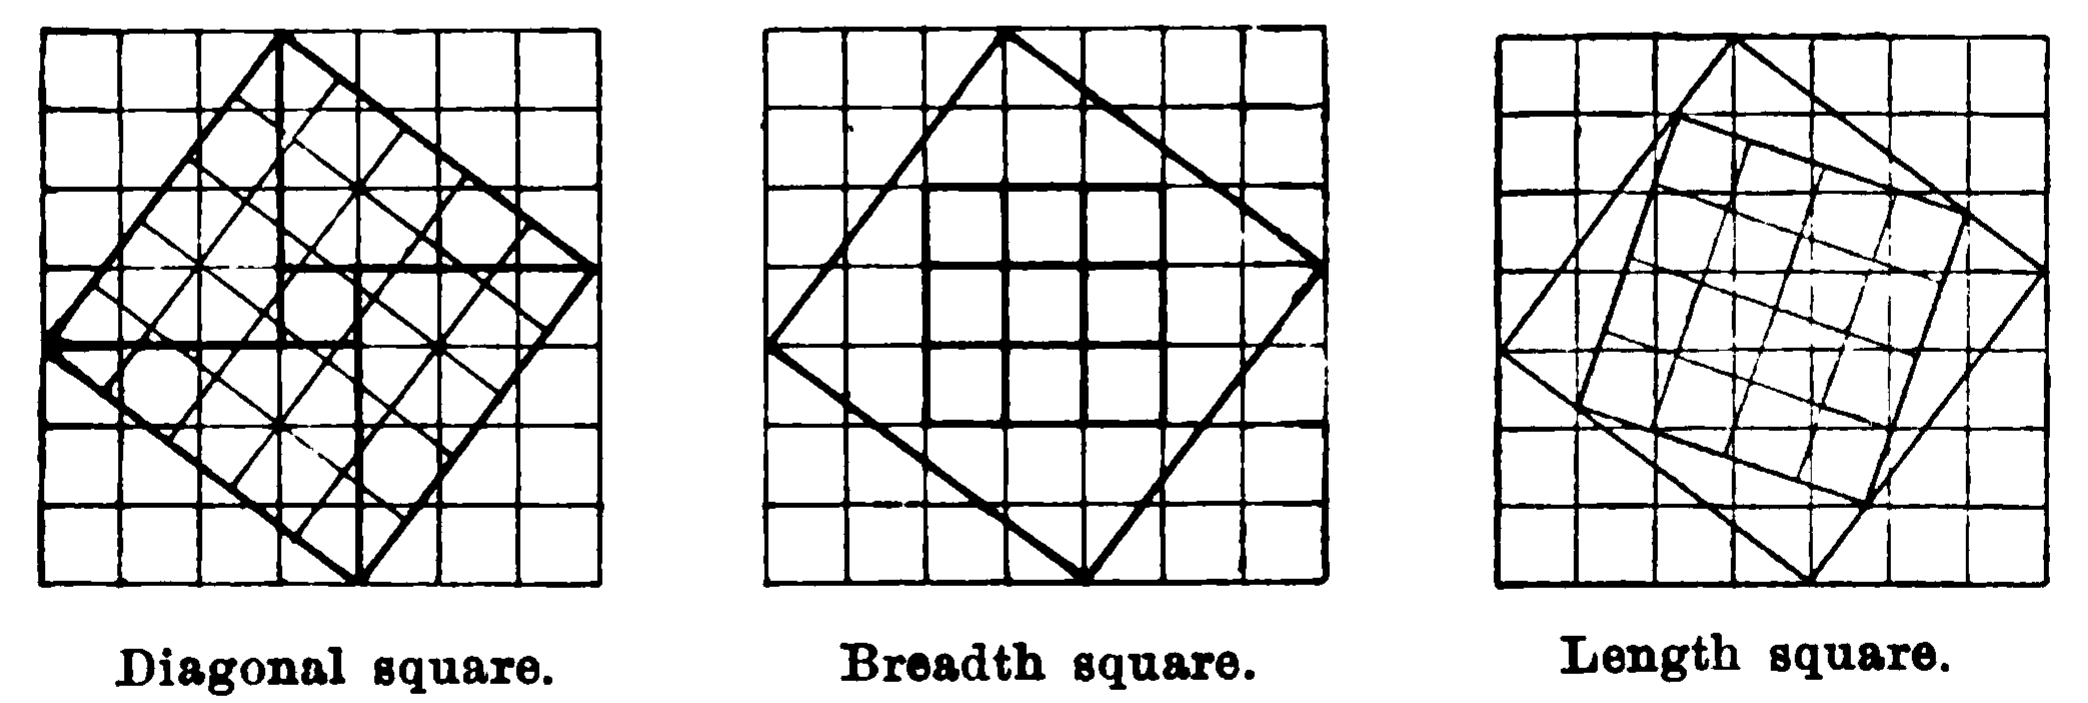
\includegraphics[width=.85\linewidth]{pdf019-chou-pei-three-diagrams.png}
\end{center}

「Chou-Kong は言った。ああ、数の術はなんと偉大であることか。あえて \emph{chü}、すなわち線尺の用法について尋ねたい。

「Shang Kao は答えた。水平の線尺は線を正し、垂直の線尺は高さを見、倒した線尺は深さを測り、横たえた線尺は距離を知るために役立つ。回した線尺は円を作り、二重の線尺は方を作る。方は
\scanfooter

\scanpage{0020}{第二章、印刷頁6}
\setcounter{footnote}{0}
地に属し、円は天に属する。天は円く、地は方である。」

ここで Chang Chun-ch'ing の注は、われわれにとってもっとも興味深い。彼は次のように述べる。「物は円いか尖っているかであり、数は奇か偶かである。動く天は円を描き、その従属する数は奇である。静止する地は方を作り、その従属する数は偶である。これらは \emph{yin-yang} の説、すなわち陽性と陰性\footnote{\emph{yin} と \emph{yang} は、中国の聖典の一つ『\emph{I-ching}』における二元論的哲学の基本原理である。語 \emph{yang} は陽性、日光、男性、増加などを意味し、\emph{yin} は陰性、影、女性、減少などを意味する。}について述べたものであって、天と地の実際の形を表すものではない。天はその限界まで見通すことができず、地はその果てまでたどることができない。それならば、どうしてそれらが円または方であると断定できようか。」

この注は、中国に長く滞在したあるキリスト教宣教師の見解と完全に一致しており、Moritz Cantor はその著作の中で、この見解を興味深い蓋然性をもつものとして採用している。\footnote{M. Cantor, \emph{Vorl. üb. Geschichte der Mathematik}, I., dritte Auflage, 1907, p. 680.} その宣教師によれば、天と地は 3 と 4 の象徴であった。さらに数 3 は円に属し、その円周は直径の三倍である。4 は自然に方に属する。そこから、天と円、地と方とのさらなる比較が従ってくる。

聖典『\emph{I-ching}』には、「天一、地二、天三、地四、天五、地六」等と述べられている。さまざまな時代の哲学者や占星家の著作に見えるこのような、また関連する諸節は、上の見解の正しさを確かなものにしているように思われる。

Shang Kao は続ける。

「方に属する数は標準として役立ち、円は方から導かれる。」

ここで Chang Chun-ch'ing は、この一節は、半円周と半径とを掛け合わせることによって円面積を方の面積のように測る、という意味であると注している。

Shang Kao はさらに言う。

「天は傘の形をしている。天は青黒く、地は黄赤い。天に属する数（あるいはむしろ形）は、
\scanfooter

\scanpage{0021}{第二章、印刷頁7}
\setcounter{footnote}{0}
青黒がその表で、赤黄がその裏であるとき、形成される。そして天と地の位置を形作る。

「ゆえに、地を知る者は賢明であり、天を知る者は聖である。\footnote{ここでは、天文学的な主題を扱うことは、すぐれた賢者でなければできない、という意味である。} 知識は影から来て、影は表または線尺から来る。線尺は数とともに、望まれるとおりに宇宙のすべてを支配し導く。

「Chou-Kong は言った。まことに見事である。」

この対話の本文から分かるように、Chou-Kong の時代の中国人は、直角三角形の辺上に描かれる平方に関する、応用上きわめて重要なピタゴラスの定理を知っていた。Euclid に見られるような簡潔な幾何学的形式では述べられていないが、それが古代中国人によって確実に確立されていたという事実は否定できない。

中国人は、しばしば古代バビロニア人と血統的に近い種族であると考えられている。後者は少なくとも辺 3、4、5 の特別な場合について同じ関係をもっていたようである。もし中国人がバビロニアの同族からその知識を借りたと仮定できるなら、なぜ逆に後者が前者から学んだと考えることができないのか。Chou-Kong より六世紀も後に活躍した Pythagoras は、東方へ旅して Babylon へ、おそらくさらに India へ行ったと言われていないだろうか。彼はその旅の途中で、のちに彼の名に結びつけられる定理を見たのではないか。何らかの未知の経路で China からもたらされたそれに出会ったのではないか。彼と Chou-Kong との間に流れた時間は、この問題をまさに未決の問いとして残す。

『\emph{Chou-pei}』の第二の対話では、学識ある Ch'ên-Tsŭ が Ying Fang に対し、Shang Kao が第一の対話で Chou-Kong に語ったよりもさらに実質的でよく組織された主題を教えている。しかし全体はもっぱら暦法または天文学の理論に関するもので、比較的後の時代のものであるから、ここで全文を挙げることはしない。ただ Ch'ên-Tsŭ の陳述の一段だけを再現する。

「太陽は夏至には南へ 16000 中国里、冬至には南へ 135000 里の位置にあり、そこでは
\scanfooter

\scanpage{0022}{第二章終結および第三章開始、印刷頁8}
\setcounter{footnote}{0}
垂直に立てた棒は正午に影を投げない。\footnote{これらの距離は、地が平らであると仮定したうえで、表の影の長さから、同書に与えられている特異な方法で推定されたものである。} したがって、二至における太陽の位置は互いに 119000 里離れており、真夜中には太陽は同じ方向に北へ同じ距離だけ離れている。ゆえに 238000 里の長さは夏至における太陽の軌道の直径を表し、その公転の長さは 714000 里である。」

Ch'ên-Tsŭ はさらに述べる。

「冬至には太陽の軌道は直径 476000 里をもち、軌道の円周は 1428000 里である。」

これらの場合、容易に分かるように、円周は直径の三倍として取られている。中国人は古くから $\pi=3$ の値を用いていた。

『\emph{Chou-pei}』に見える Lü の議論には、一年は $365\frac14$ 日から成り、円の円周は $365\frac14$ 度に分けられると述べられている。このような用法は、Lü の生きた時代よりはるか以前に生じていたものと一般に信じられている。

『\emph{Chou-pei}』第二巻には、直径 $121\cdot75$ フィートを取り、それに 3 を掛ければ $365\frac14$ フィートが得られ、これは天の円周における $365\frac14$ 度に対応する、という趣旨の一節を読む。

Lüh-Shih の考察の中には、分数による除法の例が与えられている。119000 里を $182\frac58$ 日で割るには、被除数と除数をまず除数の分母で掛ける。この場合その分母は 8 である。あるいは、単位を変えることによって両者を整数値の形にしてから除法を実行する。記述はやや曖昧な言語で与えられているが、われわれが述べた以外の意味を伝えるものではないように思われる。

\begin{center}
CHAPTER 3.\\
THE CHIU-CHANG SUAN-SHU.\\
第三章　九章算術。
\phantomsection\addcontentsline{toc}{subsection}{第3章　九章算術}
\end{center}

現在まで伝わる中国の数学書のうち、『\emph{Chou-pei}』に次いで古いものは、疑いなく『\emph{Chiu-chang Suan-shu}』すなわち「九章の算術」である。『\emph{Chou-pei}』は、厳密に言えば算術書ではないが、『\emph{Chiu-chang}』は真の算術書であり、
\scanfooter

\scanpage{0023}{第三章、印刷頁9}
\setcounter{footnote}{0}
したがって今日に残る最古の算術書である。さらにそれは、中国の古い時代に属する数学を扱うすべての著作のうち、もっとも広範で遠くまで及ぶものである。ゆえに『\emph{Chiu-chang}』は、歴史上きわめて貴重な関心をもつ。

「九章の算術」の著者も、その成立年代も、正確には知られていない。しかし、紀元三世紀に生きた注釈者 Liu Hui がその校訂本の序で記録しているところからわれわれが知りうる限り、この書は古い書きものの残片であり、Han 王朝の前期に Chang T'sang と Ching Ch'ou-ch'ang によって改訂または増補された。\footnote{Han 王朝は、皇帝 Kao-tsu が紀元前二〇二年に即位したことに始まる。この王朝は二世紀にわたり栄えたが、キリスト紀元一世紀初めに Wang Mang の簒奪によって倒された。} よく知られているように、紀元前二一三年、Ch'in 王朝の強大で専制的な皇帝 Shih Hoang-ti の勅令によって、すべての書物は焼かれ、すべての学者は生き埋めにされ、無害な算術や天文学の書物でさえ救われなかった。したがって、それより古い時代に属する算術書は残っていないのである。しかし Shih Hoang-ti の帝国は彼の死\footnote{Shih Hoang-ti は紀元前二一〇年に没した。}後まもなく崩壊し、次の Han 王朝の初めには、失われた書物が探索され、学問はまもなく復興した。この時期に Chang T'sang が現れた。注釈者 Liu Hui によれば、Chang はいくつかの古い書きものを見いだし、それをもとにして彼のつねに尊ばれる『\emph{Chiu-chang Suan-shu}』を編成した。この書はのちに Ching Ch'ou-ch'ang によって二度目の改訂を受けた。Chang がその著作を編むのに用いた原典は、Chou-Kong の命により編集された『\emph{Chiu-chang}』であったと一般に信じられているが、この事実はあまり信頼できない。Chou-Kong のそのような著作がそもそも存在したかどうかは分からない。『\emph{Chin-Shu}』\footnote{同じことは『\emph{Sui-Shu}』すなわち「Sui 王朝の記録」にも記されている。}すなわち「Chin 王朝の記録」の暦法部に読むところによれば、「九章の算術」に対する Liu Hui の注釈は、Wei 王国の王 Ch'ên-liu-Wang の治世、紀元二六三年に書かれた。同じ書に対する注釈は、七世紀に Li Ch'un-fêng によっても再び書かれた。

Chang T'sang の伝記的記事は、Szü-ma Ch'ien の『\emph{Shih-chi}』すなわち「史記」と、Pan Ku の『\emph{Han Shu}』すなわち「記録
\scanfooter

\scanpage{0024}{第三章、印刷頁10}
\setcounter{footnote}{0}
of the Han Dynasty」の中に与えられている。これらの記録によれば、ほとんど同一の内容であるが、Chang は若いころ Ch'in 政府の文官であった。その後、最初の Han 皇帝のもとで戦い、多くの輝かしい功績を挙げた。秩序が回復したのち、彼は有能な文官として仕え、紀元前一七六年には宰相となり、その地位を十四年間務めた。百歳を越えて生き、紀元前一五二年に没した。政治家として Chang は傑出した人物であり、その才能はとくに財政行政に向けられていた。彼はまた並外れた博識で知られ、とりわけ天文および占星の事柄に深く通じていた。彼は数百人の妻をかかえ、いったん子を宿した者は二度と顧みなかった。

Ching Ch'ou-ch'ang の生涯については、ほとんど、あるいはまったく何も知られていない。ただし、「Han Records」に記されているように、彼は Hsüan-Ti 帝（紀元前七三--四九年）の治世の大臣であった。

「九章の算術」の内容のうち、どれほどが Chang に、どれほどが Ching によるのか。あるいは、これらの著者が先行時代の古い遺物をどれほど利用したのか。これらの事柄については、われわれにはいかなる決定を下す手段もない。したがって、この場では、この書がどのような種類の主題を含むかを見るだけで満足しなければならない。「九章の算術」は、その名が示すように、九つの独立した巻または章から成る。以下では、九つの章の内容を順に短く記述しよう。\footnote{T. Hayashi が \emph{Brief History of Japanese Mathematics}, Nieuw Archief, Tweede Reeks, Deel VI, Derde Stuk, pp. 306--307 において述べたこれら九章の説明は、私が同書について知るところとまったく異なる。私は彼の説明の正しさについて何も知らない。}

これらの第一章は \emph{fang-t'ien}、すなわち\emph{田地測量}と題され、三角形、四辺形、円形、弓形、扇形、環形など、種々の形の田を測る規則が含まれている。

三角形の面積は、底辺に高さを掛けたものの半分として与えられる。

台形は、等脚であれそうでなかれ、二つの底辺の和の半分に高さを掛けたものである。

円の面積については四つの異なる規則が記録され、それらは
\[
\frac12 c\times \frac12 d,\qquad \frac14 cd,\qquad \frac34 d^2,\qquad \text{and}\qquad \frac1{12}c^2
\]
に等価である。ここで $c$ と $d$ は
\scanfooter

\scanpage{0025}{第三章、印刷頁11}
円周と直径を表す。この規則では $\pi$ は明らかに 3 に等しいものとして取られている。

円の弓形の面積は次のように与えられる。
\[
=\frac12\{(\text{chord})\times(\text{altitude})+(\text{altitude})^2\},
\]
また円の扇形の面積は、弧と直径との積の四分の一として与えられる。

環形の田は、内周と外周との和の半分を取り、二つの円周の間の法線距離を掛けることによって測られる。

同じ章には分数の扱いが与えられている。すなわち、\emph{yüeh-fen} は分数をその簡約形へ直すことを意味する。この操作の規則は次のように読める。「半分にできるときは半分にする。半分にできないときは、分母と分子を置き、大きい方から小さい方を引く。この過程を繰り返せば、ついに \emph{têng}、すなわち公約数を得る。この公約数で簡約せよ。」この規則は、二つの数の最大公約数を求め、それによって両方を割ることにほかならない。たとえば $\frac{49}{91}$ は $\frac{7}{13}$ に等しいとされる。

分数を加えるには、まず各分子を他の分数の分母で掛け、それからその結果を加え、その和を分母の連続積で割る。同じ分母をもつ分数の場合には、分子をただちに加え合わせればよい。

二つの分数の減法は、分子を相手の分母で掛け、二つの積のうち小さいものを大きいものから引き、その余りを分母の積で割ることによって行われる。

分数を掛けるには、分子どうし、分母どうしをそれぞれ掛け、これらの積の割り算によって求める結果へ至る。

量 $a+\frac cb$ と $a'+\frac{c'}{b'}$ との乗法は、次の分数を作ることによって行われる。
\[
\frac{(ab+c)(a'b'+c')}{bb'}.
\]

この章には分数のさらに進んだ扱いはないが、分数による除法は後の章で考察されており、適当な箇所で述べる。

第二章は \emph{su-mi} で、単純な百分率と比例の問題を扱う。
\scanfooter

\scanpage{0026}{第三章、印刷頁12}
第三章 \emph{shuai-fen} は、定められた比率に従って共同者の間に財産を分配する問題を扱う。この章の初めには次の規則が見られる。「比率を置く。それらを加え合わせ、その和を除数とする。分配されるべき総量を各比率で掛けると、それぞれの被除数を得る。こうして除法により各人の答えが得られる。」

同じ章はさらに \emph{fan-shuai} を扱う。一つの例によって、この題名の意味は明らかになる。

「紐一重が 240 文の金であるとき、1328 文で紐は何重得られるか。」

これは比例の問題にほかならない。

第四章は \emph{shao-kuang} で、その目的は、面積と一辺が与えられた長方形を決定すること、および数の平方根と立方根を評価することにある。

この章の問題では、答えは普通の分数で与えられているにもかかわらず、単位分数が用いられていることは非常に注目すべきである。たとえば、長方形の田の一辺は次のように表されている。
\[
1+\frac12+\frac13+\frac14+\frac15+\frac16+\frac17+\frac18+\frac19+\frac1{10}+\frac1{11}.
\]

この章には、分数をともなう粗い種類の除法が与えられている。説明のため、同書から一つの例とその規則を挙げる。

「幅が一歩と半歩と三分の一歩である［長方形の］田がある。［面積］が 1 \emph{pu}［240 平方歩］であるとき、その田の長さはいくらか。

「答え。$130\frac{10}{11}$ 歩。

「規則。分母に［数］3 があるので、1 は 6、半分は 3、三分の一は 2 と取らなければならない。これらを加えると 11 となり、これを \emph{fa}、すなわち除数とする。田の 240［平方］歩を置き、ここでも 1 は 6 と数えるので、この数 6 を掛ける。その積が \emph{shih}、すなわち被除数である。そこで除法を行うと、田の長さに含まれる歩数が得られる。」

以上から、分数を伴う除法は逆数を掛けることによって行われていたことが明らかである。

「九章」および他のすべての古代中国の著作には、小数の使用は見られない。

この章において与えられる平方根と立方根の求値の規則は、ほとんど理解しがたい曖昧な言葉で述べられているが、
\scanfooter

\scanpage{0027}{第三章、印刷頁13}
\setcounter{footnote}{0}
これを Sun-Tsŭ や Ch'ên Luan の著作に見える記述と比較し、さらに後代に算木が操作された方法を考え合わせると、すべての謎は疑いの跡を残さず解ける。

与えられた数の平方根の抽出は、次のように行われる。

「開かれるべき数を被除数の列に置く。

「一つの単位算木を借り、二列ごとにそれを進める\footnote{これは、与えられた数を二桁ずつの組に分けることである。}。そして（根の第一桁として）どの数が得られるべきかを考える。

「得られた数で借りた単位を掛け、その結果を除数の列に置く。

「次に（被除数と除数とで）除法を行う。

「除法が終わったら、除数を二倍し、それを定除数とする。

「新しい除数を一列戻す。

「再び単位算木を借り、前と同じように進める。

「再び、根の次の数字が何であるべきかを考える。

「それを借りた単位で掛け、その積を定除数の次に低い列へ付け加える。ついで除法を行う。

「二度目の付加を行い、前と同じ仕方で進める。」

Liu Hui の「九章」に対する注では、この過程は幾何学的に説明されているが、それは非常に不十分なものである。

古代中国人は小数を扱うことを知らなかったので、平方根における小数部分の考察は奇妙な誤りを導いた。そこで「九章算術」は次のような趣旨で進む。

「開方しても結論に至らなければ、その数は確定的には開けない。この場合には、余りを得られた根で割り、その結果を根の分数部分とする。」

しかし、「九章」には、上の規則で示されたような値を生む例は与えられていない。それが実用上どのように役立ったかは想像するしかないが、その結果はいかなるものであっただろうか。

分数部分をもつ数については、全体をまず分数の形に変換し、それから根-
\scanfooter

\scanpage{0028}{第三章、印刷頁14}
\setcounter{footnote}{0}
を抽出する操作が分子と分母の双方に適用された。ただし、分母が完全平方でない場合には、その過程を適用する前に分子・分母の双方に分母を掛ける。

「九章算術」に記された立方根抽出の過程は、ほとんど字句どおりには次のようなものである。

「与えられた数を被除数の列に置く。

「一つの単位算木を借り、三列ごとにそれを進めて、何が得られるべきかを考える。

「得られた数で借りた単位を二度掛け、その積を除数とする。ついで被除数を割る。

「除法が終わったら、除数の三倍を取り、その結果を定除数とする。それを一列戻す。

「いま得た根の数字を三倍し、その積を中間の列に置く。\footnote{これは除数の列と借りた単位との間に置かれることを意味し、もちろん除数の下に来る。}

「再び最下列に一つの単位を借りる。

「これらの項を戻し、前者は二列、後者は三列戻す。

「再び（根の次の桁として）何が得られるべきかを見積もる。それを中間の列で一度掛け、同じものを最下列で二度掛ける。これらの結果を定除数に付け加える。この列で除法を行う。

「そして次の段階でも同じように進める。

「最後に余りがあれば、操作は正確には終わらない。

「分数を付け加えるときは、まず全体を分数値に変換し、分母と分子の根を抽出する。

「分母が正確な評価を可能にしない数であるときは、両者を二度分母で掛けてから操作を行う。」

「九章」に与えられた平方根および立方根の抽出は、きわめて高い確実性をもって算木で行われたものと見える。この種の算盤については、後に Sun-Tsŭ の書の内容に関連して述べることにする。

同じ「九章」の書では、円周は面積の 12 倍の平方根に等しいとされ、球の直径は $\frac19(\text{volume})\times 16$ の立方根に等しいとされる。
\scanfooter

\scanpage{0029}{第三章、印刷頁15}
第五章は \emph{shang-kung} と呼ばれ、そこには各種の立体の体積が与えられている。

城壁、堤、防渠、濠の体積は、上幅と下幅の和の半分、高さまたは深さ、および長さを掛け合わせることによって測られる。

以下では便宜のため、次の略記を用いる。$c=$ 円周、$h=$ 高さまたは高度、$d=$ 直径、$s=$ 辺、$l=$ 長さ、$b=$ 幅、$(up.\ b)=$ 上幅、等である。すなわち、

正方柱は $=s^2h$ とされる。

円柱は $=\frac1{12}c^2h$ である。

切頭正四角錐は
\[
=\frac13\{(up.\ s)(low.\ s)+(up.\ s)^2+(low.\ s)^2\}h.
\]

円錐台は
\[
=\frac1{36}\{(up.\ c)(low.\ c)+(up.\ c)^2+(low.\ c)^2\}h.
\]

正四角錐は $=\frac13(s\text{ of base})^2h$ である。

円錐は $=\frac1{36}(\text{base }c)^2h$ である。

直三角柱は $=\frac12 blh$ である。

長方錐は $=\frac13 blh$ である。

互いに直角な二つの対辺 $a$ と $b$ をもつ四面体は、体積 $=\frac16abh$ をもつとされる。ここで $h$、すなわち高さは、その二辺の共通垂線を表す。これについて Liu Hui の注は、その図形が長方錐のちょうど半分であるために、体積はこのように測られると付け加えている。

一端の上幅と下幅がそれぞれ 10 と 6、深さが 3 で、他端は幅 8 をもち深さをもたず、長さが 7 である立体は、$=\frac16$（三つの幅の和）（深さ）（長さ）であるとされる。

下端の幅が 30、長さが 40、上端は幅をもたず長さ 20、高さが 10 である楔形は、体積 $=\frac16\{2(low.\ l)+(up.\ l)\}bh=5000$ をもつ。

この楔形をその底面に平行に切って生成される立体の体積は、
\[
=\frac16\{[2(up.\ l)+(low.\ l)]\times(up.\ b)+[2(low.\ l)+(up.\ l)](low.\ b)\}h.
\]
\scanfooter

\scanpage{0030}{第三章、印刷頁16}
この章のいくつかの問題は、異なる種類の走行の比較速度、労役の比較的な質などに関する。

第六章は \emph{chün-shu} であり、これは配分法にほかならない。この見出しのもとに集められた例を二つ挙げる。

「速い走者が 100 歩（または $a$）進む間に、遅い走者は 60 歩（または $b$）進む。いま後者が 100 歩（または $c$）先行し、前者がこれを追う。二人は何歩で追いつくか。」

答えは、$a\times c\div(a-b)=250$ 歩である。

「兎が犬より 100 歩（$a$）先を走る。犬は兎を 250 歩（$b$）追ったとき、両者は 30 歩（$c$）離れている。さらに何歩進めば犬は兎に追いつくか。」

答えは、$cb\div(a-c)=107\frac17$ 歩である。

第七章は \emph{ying-pu-tsu} と題されるが、これはときに \emph{ying-nu} とも呼ばれる。両者はいずれも\emph{盈不足}を意味する。ここにこの主題の二つの例を挙げる。

「人々が共同で物を買うとき、各人が 8 文出せば 3 文余り、各人が 7 文出せば 4 文不足する。人数と買った物の価格を知ることが求められる。」

「人々が共同で雌鶏を買うとき、各人が 9 出せば 11 余り、各人が 6 出せば 16 不足する。人数と雌鶏の価格はいくらか。」

これらの問題は、方程式
\[
y=ax-b\quad \text{and}\quad y=a'x+b'
\]
の解法に等しい。

解法の規則は次のように与えられている。

「共同購入において各人が差し出す率（$a$ および $a'$）を置く。余るもの（$b$）、または不足するもの（$b'$）をそれぞれこれらの率の下に置き、それから交差して掛ける。積を合わせれば \emph{shih} を得る。余りと不足を合わせて \emph{fa} とする。分数であれば、まず両者を同分母にする。それから \emph{shih} と \emph{fa} を率の差で割ると、その商が、買った物の価格と人数をそれぞれ表す。」

この規則に従って、まず配列 (1) を作り、そこから交差乗法によって (2) が得られ、ついで加法により (3) を得る。すなわち、
\[
(1)\quad \begin{array}{cc}a&a'\\ b&b'\end{array},\quad
(2)\quad \begin{array}{cc}ab'&a'b\\ b&b'\end{array},\quad
(3)\quad \begin{array}{c}ab+a'b\\ b+b'\end{array}.
\]
そして、価格 $=\dfrac{ab'+a'b}{a-a'}$、人数 $=\dfrac{b+b'}{a-a'}$ と取る。
\scanfooter

\scanpage{0031}{第三章、印刷頁17}
古代中国人がどのような推論によって上の解法に導かれたのかを知る手段はない。なぜなら、「九章算術」にはこの規則の構成についても他の規則についても説明が試みられていないからである。しかし、この過程がかなり代数的であることはよく分かる。すなわち、上に与えた二つの方程式から交差乗法によって絶対項を消去すると、
\[
(b'+b)y=(ab'+a'b)x,\quad \text{or}\quad \frac yx=\frac{ab'+a'b}{b+b'}
\]
を得る。また、与えられた方程式を減じると、
\[
(a-a')x-(b+b')=0,\quad \text{or}\quad x=\frac{b+b'}{a-a'}
\]
となり、$y$ の値も容易に求められる。

私が正しく推測しているなら、この解法は算木によって実行されていたように見える。

この章にはさらに、同じ場合に対する第二の規則が与えられている。それは次のようなものである。「余りと不足とを加えると、これが \emph{shih} となる。率の差が \emph{fa} である。\emph{shih} を \emph{fa} で割ると人数が得られる。これに率を掛け、余りを引くか不足を加えると、物の価格が得られる。」

ここでは、上で考えた方程式の解は、$x$ を $(b+b')\div(a-a')$ とし、$y$ を
\[
=\frac{b+b'}{a-a'}\times a-b,\quad \text{or}\quad =\frac{b+b'}{a-a'}\times a'+b'
\]
と取ることによって与えられている。

以上から、古代中国人は、この種の連立方程式を解く際に二つの異なる道を取っていたことが分かる。

方程式
\[
\left.\begin{aligned} y&=ax+b\\ y&=a'x+b'\end{aligned}\right\}\quad\text{or}\quad
\left.\begin{aligned} y&=ax-b\\ y&=a'x-b'\end{aligned}\right\}
\]
に至る問題では、第一の規則は配列 $\begin{array}{cc}a&a'\\ b&b'\end{array}$ を要求し、そこから交差乗法によって $\begin{array}{cc}ab'\sim a'b\\ b\sim b'\end{array}$ が得られる。したがって、
\[
y=\frac{ab'\sim a'b}{a\sim a'}\quad \text{and}\quad x=\frac{b\sim b'}{a\sim a'}.
\]
さらに、対応する方程式が $y=ax\pm b$ および $y=a'x$ の形である場合も考えられている。この場合、$x$ は $b\div(a\sim a')$ に等しいとされる。

\scanfooter

\scanpage{0032}{第三章、印刷頁18}
この同じ章には、次のような問題も含まれている。

「二つの水草があり、一方は初日に 3 尺、他方は 1 尺伸びる。前者の伸びは毎日その前日の半分となり、後者は前日の二倍伸びる。何日で二つは同じ高さになるか。」

この問題は盈不足法を適用して解かれている。二日では $1\cdot5$ 尺不足し、三日では $1\cdot75$ 尺余るからである。

答えは $2\frac6{13}$ 日と与えられており、そのとき両者は 4 尺と $8\frac6{13}$ 十分位の同じ高さになる。

この書にも、また中国の他の古い著作にも、算術的または幾何学的な数列の和を求める試みは見いだされない。

第八章 \emph{fang-ch'êng} は、実際には三つ以上の未知量をもつ一次連立方程式の考察である。この章が \emph{chêng} と \emph{fu}、すなわち正と負の語を用いていることは、非常に注目すべきである。

この章の第一問題は次のように読める。

「三種類の穀物があり、第一類の束三つ、第二類の束二つ、第三類の束一つで 39 升となる。第一類二つ、第二類三つ、第三類一つで 34 升となる。また第一類一つ、第二類二つ、第三類三つで 26 升となる。各類一束にはそれぞれ何升の穀が含まれているか。」

「規則。三類の束の 3、2、1 と、その穀の 39 升を右に置く。他の条件を中央と左に置く。」

したがって、その配列は添えられた図の形を取る。
\begin{center}
\fangtableA
\end{center}
本文は続ける。「右列の第一類で中央の列を乗じ、ただちに消去する。」
\scanfooter

\scanpage{0033}{第三章、印刷頁19}
これは、右列の項を、対応する中央列の項から、中央列がそのように乗じられたあとで可能な限り引く、という意味である。この操作の後の配列は、添えられたようになる。
\begin{center}\fangtableB\end{center}

「次を再び乗じ、ただちに消去する。」

これは左列について同じ操作を繰り返すことを教える。配列は今、図に示すようになる。
\begin{center}\fangtableC\end{center}

「次に、中央列に残る第二類で、ただちに消去する。」

すなわち、左列から第二類を、上に述べた過程を適用して消去するのである。結果はここに示すとおりである。
\begin{center}\fangtableD\end{center}

「消えない量について、上を \emph{fa}、すなわち除数とし、下を \emph{shih}、すなわち被除数、すなわち第三類の被除数とする。

「第二類を求めるには、除数で中央列の升数を掛け、その中から第三類の被除数を取り除く。残りを第二類の束数で割ると、第二類の被除数が得られる。

「第一類を求めるには、同じく除数で右列の升数を掛け、そこから第三類と第二類の被除数を取り除く。残りを第一類の束数で割ると、第一類の被除数が得られる。

「三つの類の被除数を除数で割れば、それぞれの升数が得られる。」

上の過程は、一見して分かるように、われわれが連立方程式
\[
3x+2y+1z=39,\qquad 2x+3y+1z=34,\qquad 1x+2y+3z=26
\]
を解く手続から大きく逸脱するものではない。
\scanfooter

\scanpage{0034}{第三章、印刷頁20}
唯一の違いは、式が今日われわれのように横の行に書かれるのではなく、縦の列に配置されることである。中国人の操作は、疑いなく、書かれた図式ではなく算木を用いて行われたように見える。

上の問題の答えは、それぞれ $9\frac14$、$4\frac14$、$2\frac34$ 升の穀として与えられている。

上の過程は、ある列の項が他の列からすべて減じられる場合にだけ直接適用できる。それでは、そのようでない場合に、古代中国人はどのように進んだのか。

次にそのような例の一つを挙げる。

「三種類の穀物がある。これら三種の穀の二束、三束、四束にそれぞれ含まれる穀は、一升を満たすには足りない。しかし、これらにそれぞれ第二、第三、第一類の一束を加えると、各場合に穀は一升ちょうどになる。では、それぞれの類の一束には何升の穀が含まれているか。」

\begin{center}
\begin{minipage}{0.58\linewidth}
\centering\fangtableE
\end{minipage}\hfill
\begin{minipage}{0.36\linewidth}
\raggedright
この問題に対応する配列は、ここに添えたものとなる。空白には配置すべき数がない。
\end{minipage}
\end{center}

答えは三類について $\frac9{25}$、$\frac7{25}$、$\frac4{25}$ 升と与えられている。

第一問題で行われたようにこの問題を解こうとすると、無から数を引く場合に出会うため、われわれは不合理に導かれる。しかし「九章」には、このような問題を考察するための規則が備わっており、解は \emph{chêng-fu-shu} の過程に従って行われる。

では、この \emph{chêng-fu-shu} とは何か。語 \emph{chêng} は\emph{正}を意味し、語 \emph{fu} は\emph{負}を意味する。したがってこれは、正数と負数の扱いであった。本文では、正数と負数、あるいはむしろ量がどのように表されたかについて何の説明も試みられていないが、Liu Hui はその注の中で、正の算木は赤色、負の算木は黒色であったと明言している。

さて、「九章」は正と負の量の扱いについて次のように説明している。
\scanfooter

\scanpage{0035}{第三章、印刷頁21}
「同名（または同符号）の量を引き、異名の量を（その絶対値で）加えるべきとき、正の量に相手がなければ、それを負とせよ。負の量に相手がなければ、それを正とせよ。異名の量を引き、同名の量を（絶対値で）加えるべきとき、正の量に相手がなければ、それを正とせよ。負の量に相手がなければ、それを負とせよ。」

これにより、「九章算術」の著者または改訂者が、あの古い時代において、正負の数または量の代数的加法と減法を知っていたことが分かる。

古代中国人は、方程式の配列において負数を用いることさえ行い、負が式の初めに現れる場合もあった。

\begin{center}
\begin{minipage}{0.28\linewidth}
\raggedright
たとえば、ある問題について、ここに示すような配列を得る。
\end{minipage}\hfill
\begin{minipage}{0.66\linewidth}
\centering\fangtableF
\end{minipage}
\end{center}

この場合、本文は次のように述べる。「二頭の牛と五頭の羊を正とし、十三頭の豚を負とし、金の余りを正と置く」、等々。

Liu Hui の注には、方程式の任意の項は必ずしも最上位のものでなくとも消去でき、減法または加法は必ずしも右から左へ実行される必要はなく、都合に応じて互いに任意の順序で行ってよい、と記されている。

第九章で最後の章は \emph{kou-ku} に関する。\emph{kou} は直角三角形の一辺であり、\emph{ku} は別の一辺である。したがって \emph{kou-ku} という語は直角三角形を意味する。この章の問題は二十四あり、その多くはピタゴラスの定理によって解けるもので、この定理は次の言葉で述べられている。

「第一辺と第二辺を平方し、それらを加える。すると、その和の平方根が \emph{hsien}、すなわち斜辺である。

「また、第二辺の平方を斜辺の平方から引けば、その余りの平方根が第一辺である。

「また、第一辺の平方を斜辺の平方から引けば、その余りの平方根が第二辺である。」
\scanfooter

\scanpage{0036}{第三章、印刷頁22}
この章に見いだされる問題のいくつかを、次に再録する。

「高さ 20 尺、周囲 3 尺の木の下に葛が生え、幹の周りを七回巻いてちょうどその頂上に達する。この葛はどれほどの長さか。」

「規則。$7\times3$ を（直角三角形の）第二辺とし、木の高さを第一辺とする。すると斜辺が葛の長さである。」

「一辺 10 尺の池の中央に葦が生えており、水面より 1 尺上に出ている。それを岸まで引くと、ちょうど岸に届く。水の深さと葦の長さを求めよ。」

この問題は、次の公式に至る規則で解かれる。
\[
(\text{depth})=\frac{(\text{half pond's side})^2-(\text{upward of water})^2}{2(\text{upward of water})},
\]
\[
(\text{reed})=(\text{depth})+(\text{upward of water}).
\]

「木の頂から紐が垂れており、その端は地上で 3 尺（$a$）のところにある。しかしそれをきつく張ると、木の根元から 8 尺（$b$）離れた点に届く。この紐の長さ（$x$）はいくらか。」

解。$x=\frac12\left(\frac{b^2}{a}+a\right)$。

「高さ 10 尺（$h$）の壁に、一本の棒がその頂で斜めにもたれている。この棒をさらに 1 尺（$d$）引けば、完全に地面に倒れる。この棒の長さはいくらか。」

解は、$\frac12\left(\frac{h^2}{d}+d\right)=55$ である。

「大きさの不明な円柱状の材木が壁の中に埋まっている。それを $\frac1{10}$ 尺深く（$a$）削ると、幅 1 尺（$b$）に広がっていることが見える。その直径を知ることが求められる。」

解法の規則は、$a+\left(\frac12 b\right)^2\div a$ が直径である、というものである。

この解は、円弓形の高さと直径との積が、弧の端とその中点とを結ぶ弦の平方に等しい、という幾何学命題に等価である。この命題は、十八世紀および十九世紀の日本の数学者によって広く参照された。
\scanfooter

\scanpage{0037}{第三章、印刷頁23}
「ある戸の高さ（$h$）は、その幅（$b$）より 6.8 尺（$l$）長く、対角線は 10 尺（$d$）である。その幅と高さはいくらか。」

この問題の解は、次の公式によって行われる。
\[
b=\sqrt{\frac12\left\{d^2-2\times\left(\frac l2\right)^2\right\}}-\frac l2,
\qquad
h=\sqrt{\frac12\left\{d^2-2\times\left(\frac l2\right)^2\right\}}+\frac l2.
\]
これらの公式の導出の仕方は疑問のままである。しかし、それらの式が文字式の二次方程式 $x^2+(x+l)^2=d^2$ の正根を表していることは分かる。

「高さと幅の分からない戸があり、長さの分からない棒がある。ただ、その棒は戸の幅より 4 尺（$a$）長く、戸の高さより 2 尺（$b$）長く、しかも戸の対角線に等しいと言われる。この三つの長さを求めることが必要である。」

ここで幅は $\sqrt{2ab}+b$、高さは $\sqrt{2ab}+a$、棒の長さは $\sqrt{2ab}+a+b$ によって与えられる。

「九章」の本文では、この規則はもちろん他のすべての規則と同じように、代数式ではなく完全な言葉で表されている。

この規則に見られる式もまた、二次方程式から生じるように思われる。

「高さ 10 尺の竹があり、その上端が折れて、幹から 3 尺離れた地面に達する。折れたところの高さはいくらか。」

これは次のように解かれる。
\[
(\text{height of break})=\frac{\text{height}}{2}-\frac{(\text{distance from stem})^2}{2(\text{height})}.
\]

この問題は、Brahmagupta の著作にも含まれていると述べられているので、われわれにとって非常に興味深い。インドの学問が中国思想にきわめて大きな影響を及ぼしたことは確かであるが、同時に中国でなされた発見が Hindoo の学者の目に触れた可能性もある。もしこの問題が二つの隣国の書物に同じ形で現れることが単なる偶然でないなら、二者のうち一方が他方から借りたに違いない。そしてこれは、中国の所産が南方の啓けた地に移された一例であるかもしれない。というのは、Brahmagupta は、われわれが今述べている中国の書の編纂より六、七世紀も後に現れたからである。

「同じ場所に二人の人が立っており、一方 $A$ は 7 進む間に、$B$ は 3 進む。$B$ は東へ出発し、$A$ は南へ 10 歩進み、
\scanfooter

\scanpage{0038}{第三章、印刷頁24}
それから斜めに進んでちょうど $B$ と一点で出会う。出会うまでに $A$ と $B$ はそれぞれ何歩歩いたか。

「答え。$B$ は $10\cdot5$ 歩、$A$ は斜めに $14\frac12$ 歩歩く。」

規則は本質的に次のように与えられている。$\frac12(7^2+3^2)$（$=a$）を $A$ の斜行の率とする。すると、$7^2$ ---（この率）（$=b$）は南行の率であり、$3\times7$（$=c$）は $B$ の歩行の率である。したがって、
\[
(A\text{'s oblique walk})=\frac{10\times a}{b},\qquad (B\text{'s walk})=\frac{10\times c}{b}.
\]

直角三角形に内接する正方形の一辺は、二辺の積をその和で割った商として与えられる。

直角三角形に内接する円の直径は、直角を挟む二辺の積の二倍を三辺の和で割った商として与えられる。

若干の問題は幾何学的比例に関する。

「一辺 200 歩の正方形の村があり、各辺の中央に門がある。東門から 15 歩外に木がある。南門から何歩出たところでそれが見えるか。」

「東西の辺が 7 里、南北の辺が 9 里である（長方形の）町があり、その四つの壁の各中央に門が一つずつ開いている。東門から 15 里のところに木がある。この木は南門からどれだけ離れたところで見えるか。」

「辺の長さが分からない正方形の町があり、各辺の中央に門が開いている。北門から 20 歩外に木があり、その木は、南門から 14 歩歩き、さらに西へ 1775 歩曲がった点から見える。一辺の長さはいくらか。」

この問題の解は非常に注目すべきである。なぜなら、通常のように公式に等しい規則によって与えられているのではなく、ただ次の方程式そのものを表す式の根を開くことによって答えが得られる、と指示されているだけだからである。
\[
x^2+(20+14)x-2\times20\times1775=0.
\]

もちろん、本文にはそのような方程式に言及するものは何も見られない。しかし、未知数の一次係数における追加の線または項を伴って、開根の操作を行うことが示唆されている可能性は非常に高い。この追加の線は算木の盤上で \emph{tsung} と呼ばれ、
\scanfooter

\scanpage{0039}{第三章終結および第四章開始、印刷頁25}
\setcounter{footnote}{0}
この術語は後の中国数学の発展において普遍的に用いられた。それは「九章」の著者が平方根抽出の過程を記述する際に初めて用いた語であった。この述べられた過程は、文字方程式ではなく数値計算にだけ適用できる。しかしこれは古代中国人の数学的到達にとって特異な出来事とみなされなければならない。なぜなら、同じ過程は、数値方程式の高次の美しい解法へと発展する運命をもっており、その高名な名は\emph{天元術}であり、これは著名な Horner の方法と同じだからである。この方法の発明については、後に再び述べる。

\begin{center}
CHAPTER 4.\quad THE SUN-TSÜ SUAN-CHING OR THE\\
ARITHMETICAL CLASSIC OF SUN-TSÜ.\\
第四章　孫子算経、または Sun-Tsŭ の算術経典。
\phantomsection\addcontentsline{toc}{subsection}{第4章　孫子算経、または Sun-Tsŭ の算術経典}
\end{center}

\emph{Sun-Tsŭ Suan-ching} は字義どおりには「Sun-Tsŭ の算術経典」を意味し、三巻から成る、体系的に整えられた著作である。この書によってこそ、古代中国人が乗法と除法という算術操作をどのように扱っていたかを知ることができる。われわれはこの書の記述に短い紙幅を割くことにする。

この著作の著者 Sun-Tsŭ の生没年代は不幸にも知られていない。彼はときに、紀元前六世紀の著名な兵法家 Sun Wu と同一人物と考えられた。Sun Wu は、尊称として普通 Sun-Tsŭ と呼ばれる人物である。学識深く著名な考古学者 Chu I-tsun（一六二九--一七〇九）はこの意見であった\footnote{Yüan's \emph{Biographical Notices}, Book 1.}が、数学者 Tai Chêng（一七二二--一七七七）は、Sun-Tsŭ の書の成立は Han の皇帝 Ming-Ti の治世より前にはさかのぼりえないと主張する。Tai Chêng は、われわれの前にあるこの書が「Chang-an」「Lo-yang」「Buddhist works」\footnote{Yüan's \emph{Biographical Notices}, Book 1.}などの語を含んでおり、これらはいずれも前 Ch'in 時代の起源ではありえない\footnote{すなわち、紀元前二世紀以前のこと。}という事実にその議論を置いている。Ming-Ti は五八年から七五年まで政治を行い、その治世中、すなわち六五年に仏教が中国に伝えられた。

上の語は、次の問題\footnote{\emph{Arithmetical Classic of Sun-Tsŭ}, Book 3.}に含まれている。

「Chang-an と Lo-yang との距離は 900 中国里である。一回転で 11 尺を測る車輪を運ぶとき、
\scanfooter

\scanpage{0040}{第四章、印刷頁26}
\setcounter{footnote}{0}
この二都市の間を行くには、何回転で足りるかを求めることが必要である。」

「29 偈から成る仏典があり、各偈は 63 文字を含む。全体で何文字含まれるかを求めることが必要である。」

Yüan Yüan（一七六四--一八四九）は、著名な政治家であり、中国の天文学者および数学者の伝記的記事に関する著作の筆者\footnote{この著作は『\emph{Ch'ou-jên Ch'uan}』と題され、われわれはこれを Yüan の「Biographical Notices」と呼ぶことにする。}であったが、他の多くの人々と同じく Tai Chêng の意見に同意している。\footnote{Yüan's ``Biographical Notices'', Book 1.} 見られるように、Sun-Tsŭ の「算術経典」の著者を兵法家 Sun Wu と同一視する何らかの表示や記録は、どこにも見いだされない。

さらに、Sun-Tsŭ の書を「九章算術」より古いものと取ることはできない。前者は記述の綿密さにおいて後者を大きく上回っている。Sun-Tsŭ は、見たところ、「九章」の内容を基礎としてその考察を進めたのであろう。

Sun-Tsŭ はその著作の序において、物質的なものも知的なものも、万物の起源を数または計算の学に帰している。

Sun-Tsŭ の書の冒頭で、彼は大数と小数、および度量衡の名称を与えている。

ここに Sun-Tsŭ の本文から引用する。

「長さの尺度は \emph{hu} から始まる。一 \emph{hu} とは何か。蚕が吐く糸は（直径において）一 \emph{hu} を測る。十 \emph{hu} が一 \emph{mi} を作り、十 \emph{mi} が一 \emph{hao}、十 \emph{hao} が一 \emph{li}、十 \emph{li} が一 \emph{fen}、十 \emph{fen} が一 \emph{t'sun}、十 \emph{t'sun} が一 \emph{ch'o} または一尺、十尺が一 \emph{chang}、十 \emph{chang} が一 \emph{yin} である。また 50 尺が一 \emph{tuan}、40 尺が一 \emph{p'i}、6 尺が一 \emph{p'ou} または一歩、240 歩が一 \emph{mou}、300 歩が一 \emph{li} または一中国里である。

「重さは一粒の panicum maliaceum から始まる。このような粒十個が一 \emph{t'sen}、十 \emph{t'sen} が一 \emph{shu}、24 \emph{shu} が一 \emph{liang}、16 \emph{liang} が一 \emph{chin}、30 \emph{chin} が一 \emph{chün}、4 \emph{chün} が一 \emph{shih} である。

「容積は一つの \emph{su}、すなわち粟の一粒に始まる。このような粒六つが一 \emph{kuei}、十 \emph{kuei} が一 \emph{t'so}、十 \emph{t'so} が一 \emph{ch'ao}、十 \emph{ch'ao} が一 \emph{shao}、十 \emph{shao} が一 \emph{ho}、十 \emph{ho} が一 \emph{shong}、十 \emph{shong} が一 \emph{tou}、十 \emph{tou} が一 \emph{hu} で、これは粟 60000000 粒を含む。」

Sun-Tsŭ の大数の概念は、見たところ非常に不完全であった。彼は言う、十千の十千が一 \emph{i} を作る、と。
\scanfooter



\newcommand{\rodv}[1]{\begin{tikzpicture}[baseline=-.15em,scale=.35,line width=.8pt,line cap=round]\foreach \i in {1,...,#1}{\draw (\i*.28,0)--(\i*.28,1.05);}\end{tikzpicture}}
\newcommand{\rodh}[1]{\begin{tikzpicture}[baseline=.2em,scale=.35,line width=.8pt,line cap=round]\foreach \i in {1,...,#1}{\draw (0,\i*.22)--(1.2,\i*.22);}\end{tikzpicture}}
\newcommand{\rodunit}[1]{\begin{tikzpicture}[baseline=-.15em,scale=.35,line width=.8pt,line cap=round]
  \ifnum#1<6\foreach \i in {1,...,#1}{\draw (\i*.28,0)--(\i*.28,1.05);}\else\pgfmathtruncatemacro{\vv}{#1-5}\draw (0,1.05)--(1.25,1.05);\foreach \i in {1,...,\vv}{\draw (\i*.28,0)--(\i*.28,.85);}\fi
\end{tikzpicture}}
\newcommand{\rodten}[1]{\begin{tikzpicture}[baseline=-.15em,scale=.35,line width=.8pt,line cap=round]
  \ifnum#1<6\foreach \i in {1,...,#1}{\draw (0,\i*.22)--(1.2,\i*.22);}\else\pgfmathtruncatemacro{\hh}{#1-5}\draw (.6,.2)--(.6,1.25);\foreach \i in {1,...,\hh}{\draw (0,\i*.22)--(1.2,\i*.22);}\fi
\end{tikzpicture}}
\newcommand{\rodnumsunit}{\begin{center}\begin{tabular}{ccccccccc}\rodunit{1}&\rodunit{2}&\rodunit{3}&\rodunit{4}&\rodunit{5}&\rodunit{6}&\rodunit{7}&\rodunit{8}&\rodunit{9}\\[-1mm]1&2&3&4&5&6&7&8&9\end{tabular}\end{center}}
\newcommand{\rodnumstens}{\begin{center}\begin{tabular}{ccccccccc}\rodten{1}&\rodten{2}&\rodten{3}&\rodten{4}&\rodten{5}&\rodten{6}&\rodten{7}&\rodten{8}&\rodten{9}\end{tabular}\end{center}}
\newcommand{\rodnumberAnnexed}{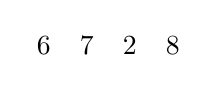
\begin{tikzpicture}[baseline=-.5em,scale=.42,line width=.8pt,line cap=round]
  \node at (0,0) {\rodten{6}}; \node at (1.3,0) {\rodunit{7}}; \node at (2.6,0) {\rodten{2}}; \node at (3.9,0) {\rodunit{8}};
\end{tikzpicture}}
\newcommand{\sqrttableA}{\begin{center}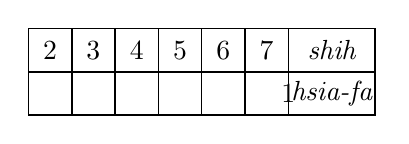
\begin{tikzpicture}[scale=.55,line width=.55pt]
\draw (0,0) rectangle (8,2);\foreach \x in {1,...,6}{\draw (\x,0)--(\x,2);}\draw (0,1)--(8,1);
\foreach \x/\t in {0.5/2,1.5/3,2.5/4,3.5/5,4.5/6,5.5/7}{\node at (\x,1.5){\t};}
\node[font=\itshape] at (7,1.5){shih};\node at (6,.5){1};\node[font=\itshape] at (7,.5){hsia-fa};
\end{tikzpicture}\end{center}}
\newcommand{\sqrttableB}{\begin{center}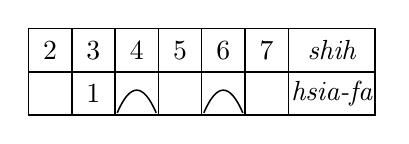
\begin{tikzpicture}[scale=.55,line width=.55pt]
\draw (0,0) rectangle (8,2);\foreach \x in {1,...,6}{\draw (\x,0)--(\x,2);}\draw (0,1)--(8,1);
\foreach \x/\t in {0.5/2,1.5/3,2.5/4,3.5/5,4.5/6,5.5/7}{\node at (\x,1.5){\t};}
\node[font=\itshape] at (7,1.5){shih};\node at (1.5,.5){1};\draw (2.05,.05)..controls(2.35,.75)and(2.65,.75)..(2.95,.05);\draw (4.05,.05)..controls(4.35,.75)and(4.65,.75)..(4.95,.05);\node[font=\itshape] at (7,.5){hsia-fa};
\end{tikzpicture}\end{center}}
\newcommand{\sqrttableC}{\begin{center}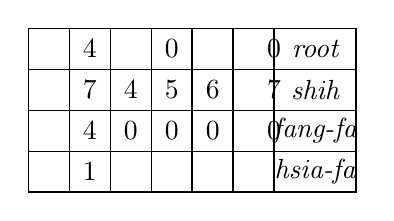
\begin{tikzpicture}[scale=.52,line width=.55pt]
\draw (0,0) rectangle (8,4);\foreach \x in {1,...,6}{\draw (\x,0)--(\x,4);}\foreach \y in {1,...,3}{\draw (0,\y)--(8,\y);} 
\node at (1.5,3.5){4};\node at (3.5,3.5){0};\node at (6,3.5){0};\node[font=\itshape] at (7,3.5){root};
\node at (1.5,2.5){7};\node at (2.5,2.5){4};\node at (3.5,2.5){5};\node at (4.5,2.5){6};\node at (6,2.5){7};\node[font=\itshape] at (7,2.5){shih};
\node at (1.5,1.5){4};\node at (2.5,1.5){0};\node at (3.5,1.5){0};\node at (4.5,1.5){0};\node at (6,1.5){0};\node[font=\itshape] at (7,1.5){fang-fa};
\node at (1.5,.5){1};\node[font=\itshape] at (7,.5){hsia-fa};
\end{tikzpicture}\end{center}}
\newcommand{\sqrttableD}{\begin{center}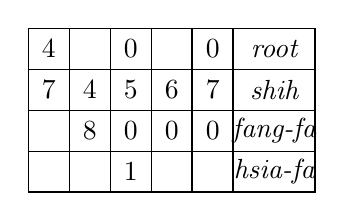
\begin{tikzpicture}[scale=.52,line width=.55pt]
\draw (0,0) rectangle (7,4);\foreach \x in {1,...,5}{\draw (\x,0)--(\x,4);}\foreach \y in {1,...,3}{\draw (0,\y)--(7,\y);} 
\node at (.5,3.5){4};\node at (2.5,3.5){0};\node at (4.5,3.5){0};\node[font=\itshape] at (6,3.5){root};
\node at (.5,2.5){7};\node at (1.5,2.5){4};\node at (2.5,2.5){5};\node at (3.5,2.5){6};\node at (4.5,2.5){7};\node[font=\itshape] at (6,2.5){shih};
\node at (1.5,1.5){8};\node at (2.5,1.5){0};\node at (3.5,1.5){0};\node at (4.5,1.5){0};\node[font=\itshape] at (6,1.5){fang-fa};
\node at (2.5,.5){1};\node[font=\itshape] at (6,.5){hsia-fa};
\end{tikzpicture}\end{center}}
\newcommand{\sqrttableE}{\begin{center}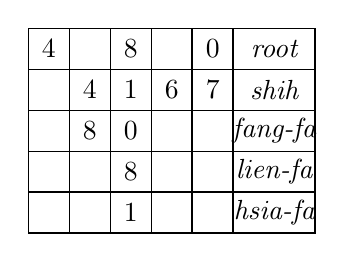
\begin{tikzpicture}[scale=.52,line width=.55pt]
\draw (0,0) rectangle (7,5);\foreach \x in {1,...,5}{\draw (\x,0)--(\x,5);}\foreach \y in {1,...,4}{\draw (0,\y)--(7,\y);} 
\node at (.5,4.5){4};\node at (2.5,4.5){8};\node at (4.5,4.5){0};\node[font=\itshape] at (6,4.5){root};
\node at (1.5,3.5){4};\node at (2.5,3.5){1};\node at (3.5,3.5){6};\node at (4.5,3.5){7};\node[font=\itshape] at (6,3.5){shih};
\node at (1.5,2.5){8};\node at (2.5,2.5){0};\node[font=\itshape] at (6,2.5){fang-fa};
\node at (2.5,1.5){8};\node[font=\itshape] at (6,1.5){lien-fa};
\node at (2.5,.5){1};\node[font=\itshape] at (6,.5){hsia-fa};
\end{tikzpicture}\end{center}}
\newcommand{\sqrttableF}{\begin{center}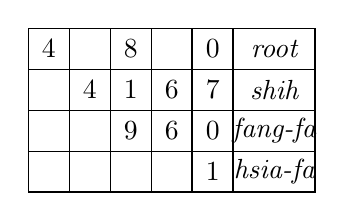
\begin{tikzpicture}[scale=.52,line width=.55pt]
\draw (0,0) rectangle (7,4);\foreach \x in {1,...,5}{\draw (\x,0)--(\x,4);}\foreach \y in {1,...,3}{\draw (0,\y)--(7,\y);} 
\node at (.5,3.5){4};\node at (2.5,3.5){8};\node at (4.5,3.5){0};\node[font=\itshape] at (6,3.5){root};
\node at (1.5,2.5){4};\node at (2.5,2.5){1};\node at (3.5,2.5){6};\node at (4.5,2.5){7};\node[font=\itshape] at (6,2.5){shih};
\node at (2.5,1.5){9};\node at (3.5,1.5){6};\node at (4.5,1.5){0};\node[font=\itshape] at (6,1.5){fang-fa};
\node at (4.5,.5){1};\node[font=\itshape] at (6,.5){hsia-fa};
\end{tikzpicture}\end{center}}
\newcommand{\sqrttableG}{\begin{center}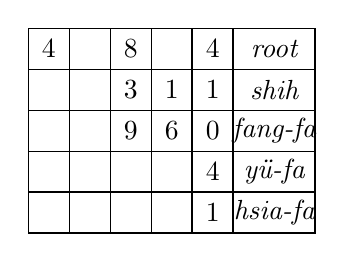
\begin{tikzpicture}[scale=.52,line width=.55pt]
\draw (0,0) rectangle (7,5);\foreach \x in {1,...,5}{\draw (\x,0)--(\x,5);}\foreach \y in {1,...,4}{\draw (0,\y)--(7,\y);} 
\node at (.5,4.5){4};\node at (2.5,4.5){8};\node at (4.5,4.5){4};\node[font=\itshape] at (6,4.5){root};
\node at (2.5,3.5){3};\node at (3.5,3.5){1};\node at (4.5,3.5){1};\node[font=\itshape] at (6,3.5){shih};
\node at (2.5,2.5){9};\node at (3.5,2.5){6};\node at (4.5,2.5){0};\node[font=\itshape] at (6,2.5){fang-fa};
\node at (4.5,1.5){4};\node[font=\itshape] at (6,1.5){yü-fa};
\node at (4.5,.5){1};\node[font=\itshape] at (6,.5){hsia-fa};
\end{tikzpicture}\end{center}}
\newcommand{\seaislandfig}{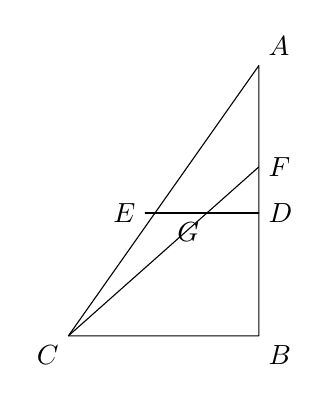
\begin{tikzpicture}[scale=.78,line cap=round,line join=round]
\coordinate (C) at (0,0);\coordinate (B) at (3.1,0);\coordinate (A) at (3.1,4.4);\coordinate (D) at (3.1,2.0);\coordinate (F) at (3.1,2.75);\coordinate (E) at (1.25,2.0);\coordinate (G) at (1.95,2.0);
\draw (C)--(B)--(A)--cycle;\draw (C)--(F);\draw (E)--(D);\node[above right] at (A){$A$};\node[below right] at (B){$B$};\node[below left] at (C){$C$};\node[left] at (E){$E$};\node[right] at (D){$D$};\node[right] at (F){$F$};\node[below] at (G){$G$};
\end{tikzpicture}}
\newcommand{\quadtable}{\begin{center}\begin{tabular}{|c|c|}\hline $-\left(c^2-\dfrac{r}{h}\times36\right)$&$x^0$\\\hline $c$&$x^1$\\\hline $1$&$x^2$\\\hline\end{tabular}\end{center}}
\renewcommand{\sqrttableA}{\begin{center}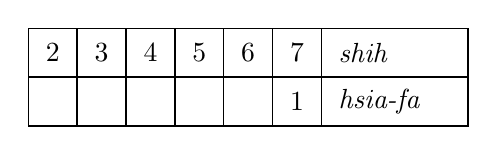
\begin{tikzpicture}[scale=.62,line width=.55pt]
\draw (0,0) rectangle (9,2);\foreach \x in {1,...,6}{\draw (\x,0)--(\x,2);}\draw (0,1)--(9,1);
\foreach \x/\t in {0.5/2,1.5/3,2.5/4,3.5/5,4.5/6,5.5/7}{\node at (\x,1.5){\t};}
\node[font=\itshape,anchor=west] at (6.15,1.5){shih};\node at (5.5,.5){1};\node[font=\itshape,anchor=west] at (6.15,.5){hsia-fa};
\end{tikzpicture}\end{center}}
\renewcommand{\sqrttableB}{\begin{center}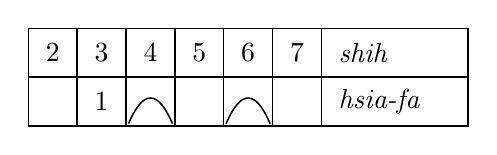
\begin{tikzpicture}[scale=.62,line width=.55pt]
\draw (0,0) rectangle (9,2);\foreach \x in {1,...,6}{\draw (\x,0)--(\x,2);}\draw (0,1)--(9,1);
\foreach \x/\t in {0.5/2,1.5/3,2.5/4,3.5/5,4.5/6,5.5/7}{\node at (\x,1.5){\t};}
\node[font=\itshape,anchor=west] at (6.15,1.5){shih};\node at (1.5,.5){1};\draw (2.05,.05)..controls(2.35,.75)and(2.65,.75)..(2.95,.05);\draw (4.05,.05)..controls(4.35,.75)and(4.65,.75)..(4.95,.05);\node[font=\itshape,anchor=west] at (6.15,.5){hsia-fa};
\end{tikzpicture}\end{center}}
\renewcommand{\sqrttableC}{\begin{center}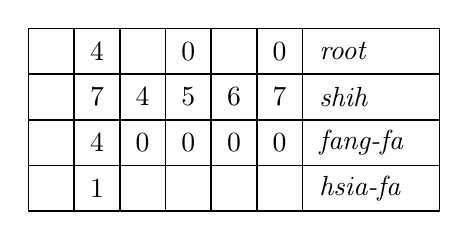
\begin{tikzpicture}[scale=.58,line width=.55pt]
\draw (0,0) rectangle (9,4);\foreach \x in {1,...,6}{\draw (\x,0)--(\x,4);}\foreach \y in {1,...,3}{\draw (0,\y)--(9,\y);} 
\node at (1.5,3.5){4};\node at (3.5,3.5){0};\node at (5.5,3.5){0};\node[font=\itshape,anchor=west] at (6.15,3.5){root};
\node at (1.5,2.5){7};\node at (2.5,2.5){4};\node at (3.5,2.5){5};\node at (4.5,2.5){6};\node at (5.5,2.5){7};\node[font=\itshape,anchor=west] at (6.15,2.5){shih};
\node at (1.5,1.5){4};\node at (2.5,1.5){0};\node at (3.5,1.5){0};\node at (4.5,1.5){0};\node at (5.5,1.5){0};\node[font=\itshape,anchor=west] at (6.15,1.5){fang-fa};
\node at (1.5,.5){1};\node[font=\itshape,anchor=west] at (6.15,.5){hsia-fa};
\end{tikzpicture}\end{center}}
\renewcommand{\sqrttableD}{\begin{center}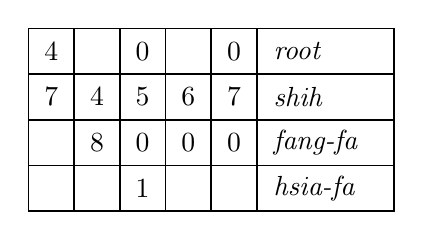
\begin{tikzpicture}[scale=.58,line width=.55pt]
\draw (0,0) rectangle (8,4);\foreach \x in {1,...,5}{\draw (\x,0)--(\x,4);}\foreach \y in {1,...,3}{\draw (0,\y)--(8,\y);} 
\node at (.5,3.5){4};\node at (2.5,3.5){0};\node at (4.5,3.5){0};\node[font=\itshape,anchor=west] at (5.15,3.5){root};
\node at (.5,2.5){7};\node at (1.5,2.5){4};\node at (2.5,2.5){5};\node at (3.5,2.5){6};\node at (4.5,2.5){7};\node[font=\itshape,anchor=west] at (5.15,2.5){shih};
\node at (1.5,1.5){8};\node at (2.5,1.5){0};\node at (3.5,1.5){0};\node at (4.5,1.5){0};\node[font=\itshape,anchor=west] at (5.15,1.5){fang-fa};
\node at (2.5,.5){1};\node[font=\itshape,anchor=west] at (5.15,.5){hsia-fa};
\end{tikzpicture}\end{center}}
\renewcommand{\sqrttableE}{\begin{center}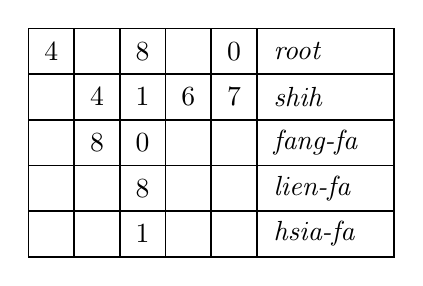
\begin{tikzpicture}[scale=.58,line width=.55pt]
\draw (0,0) rectangle (8,5);\foreach \x in {1,...,5}{\draw (\x,0)--(\x,5);}\foreach \y in {1,...,4}{\draw (0,\y)--(8,\y);} 
\node at (.5,4.5){4};\node at (2.5,4.5){8};\node at (4.5,4.5){0};\node[font=\itshape,anchor=west] at (5.15,4.5){root};
\node at (1.5,3.5){4};\node at (2.5,3.5){1};\node at (3.5,3.5){6};\node at (4.5,3.5){7};\node[font=\itshape,anchor=west] at (5.15,3.5){shih};
\node at (1.5,2.5){8};\node at (2.5,2.5){0};\node[font=\itshape,anchor=west] at (5.15,2.5){fang-fa};
\node at (2.5,1.5){8};\node[font=\itshape,anchor=west] at (5.15,1.5){lien-fa};
\node at (2.5,.5){1};\node[font=\itshape,anchor=west] at (5.15,.5){hsia-fa};
\end{tikzpicture}\end{center}}
\renewcommand{\sqrttableF}{\begin{center}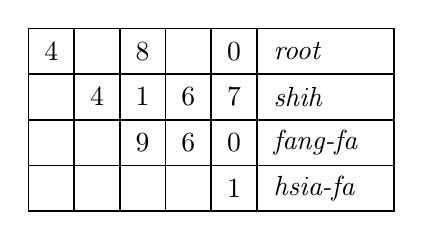
\begin{tikzpicture}[scale=.58,line width=.55pt]
\draw (0,0) rectangle (8,4);\foreach \x in {1,...,5}{\draw (\x,0)--(\x,4);}\foreach \y in {1,...,3}{\draw (0,\y)--(8,\y);} 
\node at (.5,3.5){4};\node at (2.5,3.5){8};\node at (4.5,3.5){0};\node[font=\itshape,anchor=west] at (5.15,3.5){root};
\node at (1.5,2.5){4};\node at (2.5,2.5){1};\node at (3.5,2.5){6};\node at (4.5,2.5){7};\node[font=\itshape,anchor=west] at (5.15,2.5){shih};
\node at (2.5,1.5){9};\node at (3.5,1.5){6};\node at (4.5,1.5){0};\node[font=\itshape,anchor=west] at (5.15,1.5){fang-fa};
\node at (4.5,.5){1};\node[font=\itshape,anchor=west] at (5.15,.5){hsia-fa};
\end{tikzpicture}\end{center}}
\renewcommand{\sqrttableG}{\begin{center}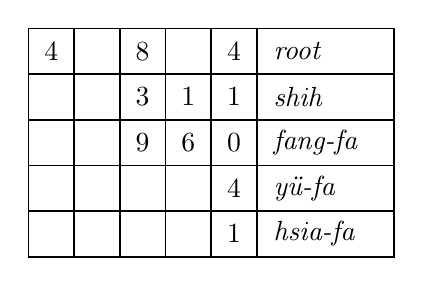
\begin{tikzpicture}[scale=.58,line width=.55pt]
\draw (0,0) rectangle (8,5);\foreach \x in {1,...,5}{\draw (\x,0)--(\x,5);}\foreach \y in {1,...,4}{\draw (0,\y)--(8,\y);} 
\node at (.5,4.5){4};\node at (2.5,4.5){8};\node at (4.5,4.5){4};\node[font=\itshape,anchor=west] at (5.15,4.5){root};
\node at (2.5,3.5){3};\node at (3.5,3.5){1};\node at (4.5,3.5){1};\node[font=\itshape,anchor=west] at (5.15,3.5){shih};
\node at (2.5,2.5){9};\node at (3.5,2.5){6};\node at (4.5,2.5){0};\node[font=\itshape,anchor=west] at (5.15,2.5){fang-fa};
\node at (4.5,1.5){4};\node[font=\itshape,anchor=west] at (5.15,1.5){yü-fa};
\node at (4.5,.5){1};\node[font=\itshape,anchor=west] at (5.15,.5){hsia-fa};
\end{tikzpicture}\end{center}}

\scanpage{0041}{第四章、印刷頁27}

一つの \,\emph{i}\, の一万倍の一万倍で一つの \emph{chao} となり、以下同様である。一方で彼は次のようにも数える。粟粒一 \emph{hu} は六万の一万倍であり、十 \emph{hu} は六 \emph{i}、百 \emph{hu} は六 \emph{chao}、等々である。

Sun-Tsŭ は $\pi=3$ とし、正方形の辺と対角線との比を 5 対 7 とする。

金、銀、玉、銅、鉛、鉄、石の重さは、それぞれ一 \emph{t'sun} 立方につき、一 \emph{chin}、14、12、$7\frac{1}{2}$、$9\frac{1}{2}$、6、3 \emph{liangs} と与えられている。

Sun-Tsŭ は算木の使用を明示的には説明しないが、彼がその書の第一巻に記すところは、この種のそろばんへの依拠がなされていたことを明らかに示すように思われる。

算木は、小さな竹または木の片で作られ、赤と黒の二色が正数と負数を表した。数学の後代の発展において用いられた算木は、長さがおよそ $1\frac{1}{2}$ インチ、幅がその長さの六分の一であった。しかし古い時代には、竹で作られたはるかに長い算木が用いられていたことが、紀元一世紀末に班固が著した『\emph{Han Shu}』に記されている。中国で算木がどれほど長く用いられていたかは確実ではないが、それが漢代になって初めて用いられたものでないことは確かである。それは、おそらく太古以来、中国で使用されていた。著名な書『\emph{Tso Ch'uan}』中の一節はこの見方を確認するものであり、そこに語られる事件は紀元前五四二年の出来事に関係している。

Sun-Tsŭ はその書の第一巻で次のようにいう。

「計算をするにあたっては、まず数の位置を知らなければならない。一は縦、十は横であり、百は立ち、千は横たわる。千と十とは同じように見え、同じく一万と百とも同じように見える。」

Sun-Tsŭ におけるこの段階は、算木の配列の記述にほかならない。これらの算木は普通、次のように配列される。

初めの五つの数は、縦に置かれた算木 1、2、3、4、5 本によって表される。一方、6 から 9 までの数の配列では、縦の算木の上に横に置かれた一本を載せ、その横の一本を 5 とする。すなわち、

\begin{center}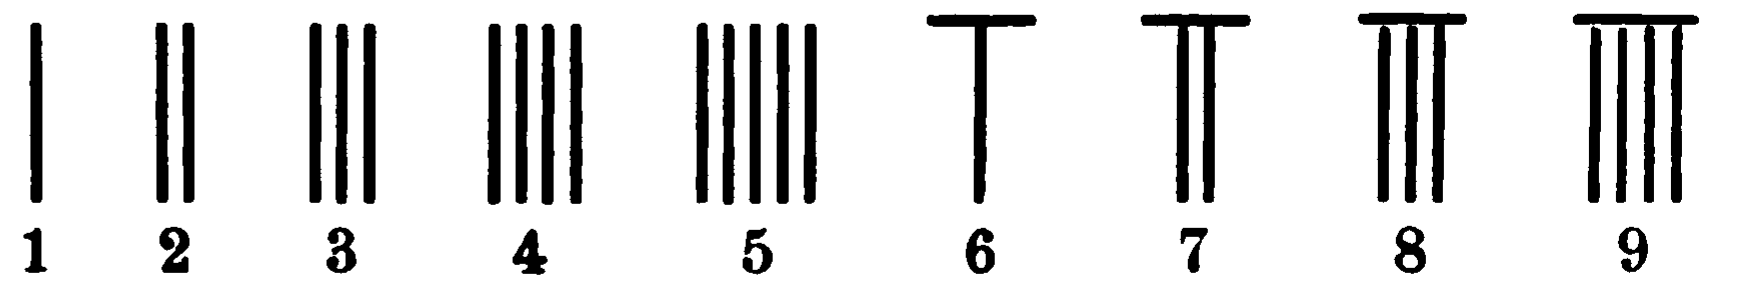
\includegraphics[width=.70\linewidth]{pdf041-rod-numerals-units.png}\end{center}

この配列法は、いま引用した箇所の次に続く段落において、Sun-Tsŭ の書に言及されている。そしてそれはまた、
\scanfooter

\scanpage{0042}{第一部、印刷頁28}

上に述べた『\emph{Tso Ch'uan}』の不明瞭な一節から推測し得るところともよく一致している。さらにこれは、後世においても従われたまさにその方法であった。

十の桁における数字は、算木によって次のように配列される。

\begin{center}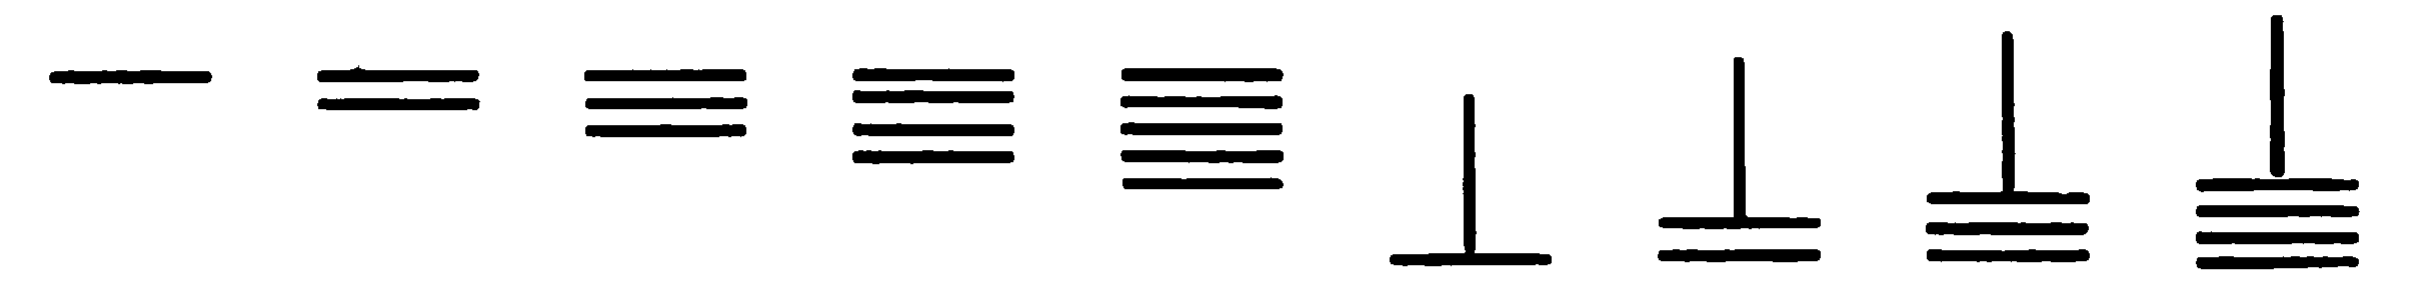
\includegraphics[width=.86\linewidth]{pdf042-rod-numerals-tens.png}\end{center}

百およびさらに高位の数については、これらの配列が交互に繰り返されるだけで、新しいことは何も加わらない。したがって 6728 という数は、添えたように配列される。

\begin{center}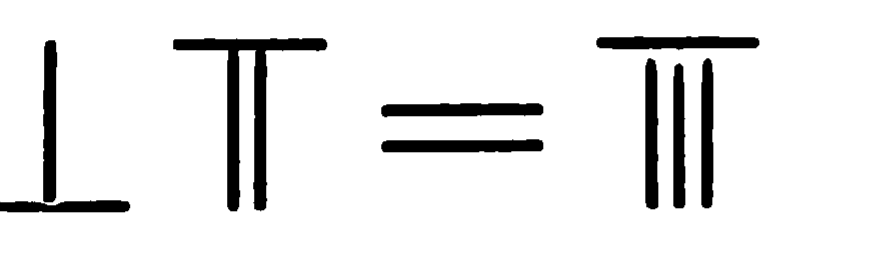
\includegraphics[width=.32\linewidth]{pdf042-rod-number-6728.png}\end{center}

二つの数を掛け合わせるために、Sun-Tsŭ は、これらの数を上下に重ねて、下の数の一の位が上の数の最高位の桁の直下に来るように配列せよ、と指示する。その最高位の桁をまず下の数で掛け、そのようにして得られた部分積を二つの数の間に来る行に配列する。次に、上の数の最高位の桁を消し、その下の数を一桁引き戻す。そこで上の数の第二の最高位の桁を下の数で掛け、部分積を中間の行に入れるが、その行はこのようにして正される。この修正は、数がすべて可動の算木で配列されているので、さほど難しくない。このように進めると、過程の最後に最終の答が得られる。

除法においては、Sun-Tsŭ の述べるところによれば、乗法の場合と異なり、商は中間の行、すなわち被除数と除数の間には置かれず、最上段の行に置かれる。たとえば 100 を 6 で割るには、これらの数を重ねて配列し、除数を他方の下に置く。この場合、除数を二つの位置または列だけ進め、百の位の下に置いて除法を試みる。しかし 1 は 6 で割れない。除数が被除数より大きいからである。それゆえ十の位へ引き戻し、最上段に商として 1 を置き、最下段の除数をそれに掛けると、被除数から $1\times 6=6$ を消すことができる。それから除数を一列引き戻し、同様に続ける。除法が終わった後に余りがあるときは、その余りを除数で割った商を、商の分数部分として取る。
\scanfooter

\scanpage{0043}{第四章、印刷頁29}

二桁以上の除数による除法は、Sun-Tsŭ の経典では説明されていない。ただし、そのような例をいくつか含んではいる。

分数は Sun-Tsŭ の第二巻で扱われている。

分数を最簡形にすることは、二つの項の最大公約数を求めることによって行われる。これは「九章算術」で見られるのと同じである。しかし Sun-Tsŭ は、分母を下段に、分子を上段に配列すべきであると述べている。

二つの分数を加える場合、Sun-Tsŭ は、分母を右に、分子を左に配列し、それから分母を分子へ交差して掛け、その積の和を分子とし、右欄の分母の積を結果の分数の分母とすることを示している。

Sun-Tsŭ は、円の面積を $\dfrac{c}{2}\times\dfrac{d}{2}$、$\dfrac{c^2}{12}$、または $d^2\times\dfrac{3}{4}$ とする。ここで $d$ と $c$ は直径と円周を表す。

Sun-Tsŭ の第二巻に見られる平方根抽出の説明は、「九章」におけるものとほとんど異ならないとはいえ、意味においてはきわめて明瞭であり、後者の不明瞭な言葉遣いとは対照的である。ここで用いられる術語は、後年、中国および日本の双方で通用するようになったものと同じであった。ただし、それらが Sun-Tsŭ によって用いられたのと同じ意味であったとは限らない。そこで本文から次の規則を引用してみよう。

「面積 234567 平方歩を配列し、これを \emph{shih} とする。

「次に一の算子を借りて、これを \emph{hsia-fa} とする。」\footnote{語 \emph{hsia} は下または下方を意味する。}

すなわち、

\begin{center}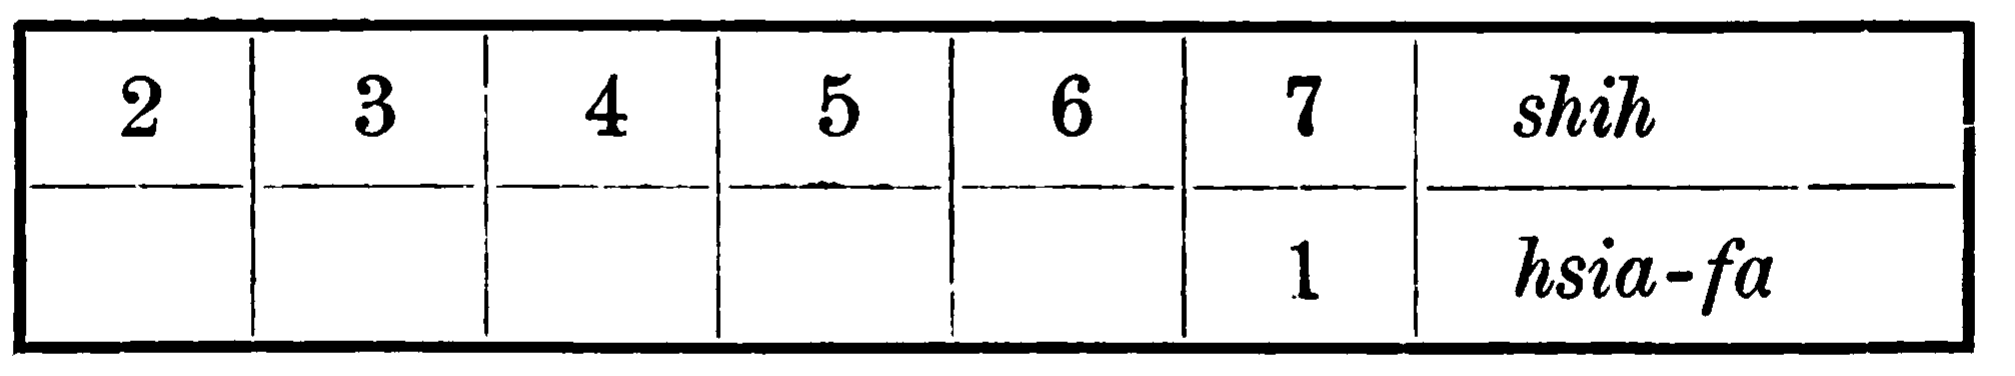
\includegraphics[width=.80\linewidth]{pdf043-sqrt-table-a.png}\end{center}

「これを一列ごとに進め、それによって \emph{shih} を組に分け、百の位に達するまで進める。」すなわち、

\begin{center}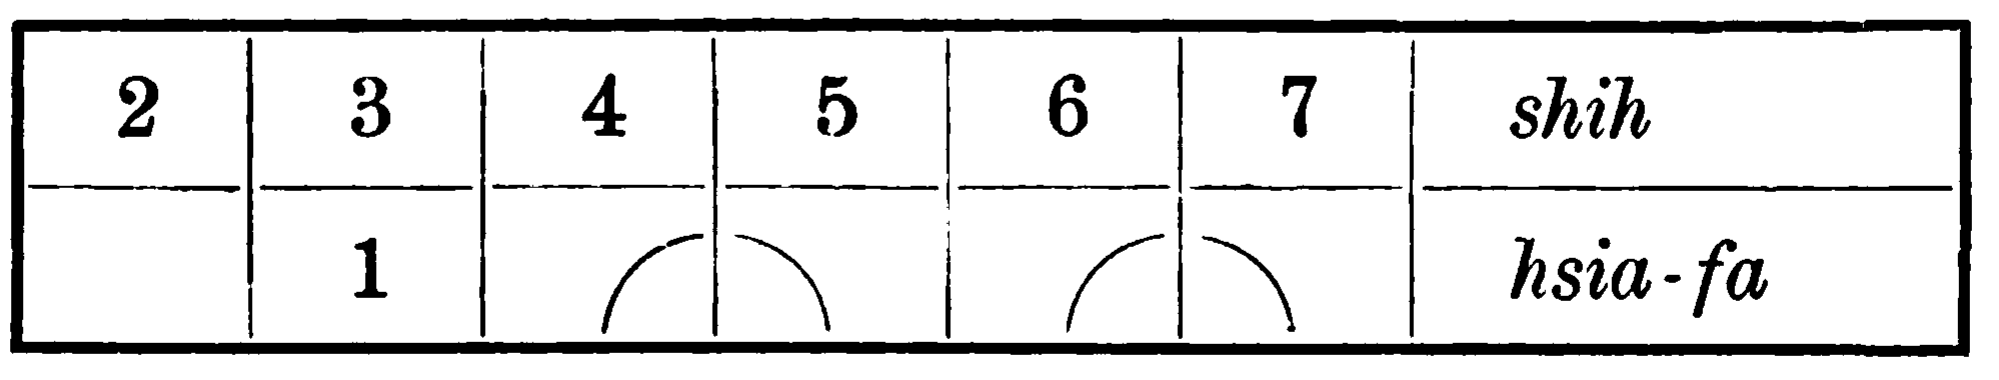
\includegraphics[width=.80\linewidth]{pdf043-sqrt-table-b.png}\end{center}

「\emph{shang}、すなわち根 400 を \emph{shih} の上に配列する。
\scanfooter

\scanpage{0044}{第一部、印刷頁30}

「40000\footnote{これは根と \emph{hsia-fa} との積である。} を \emph{shih} の下、かつ \emph{hsia-fa} の上に添え、これを \emph{fang-fa} とする。

「これを用いて根 400 を掛け、その積を \emph{shih} から引く。」すなわち、

\begin{center}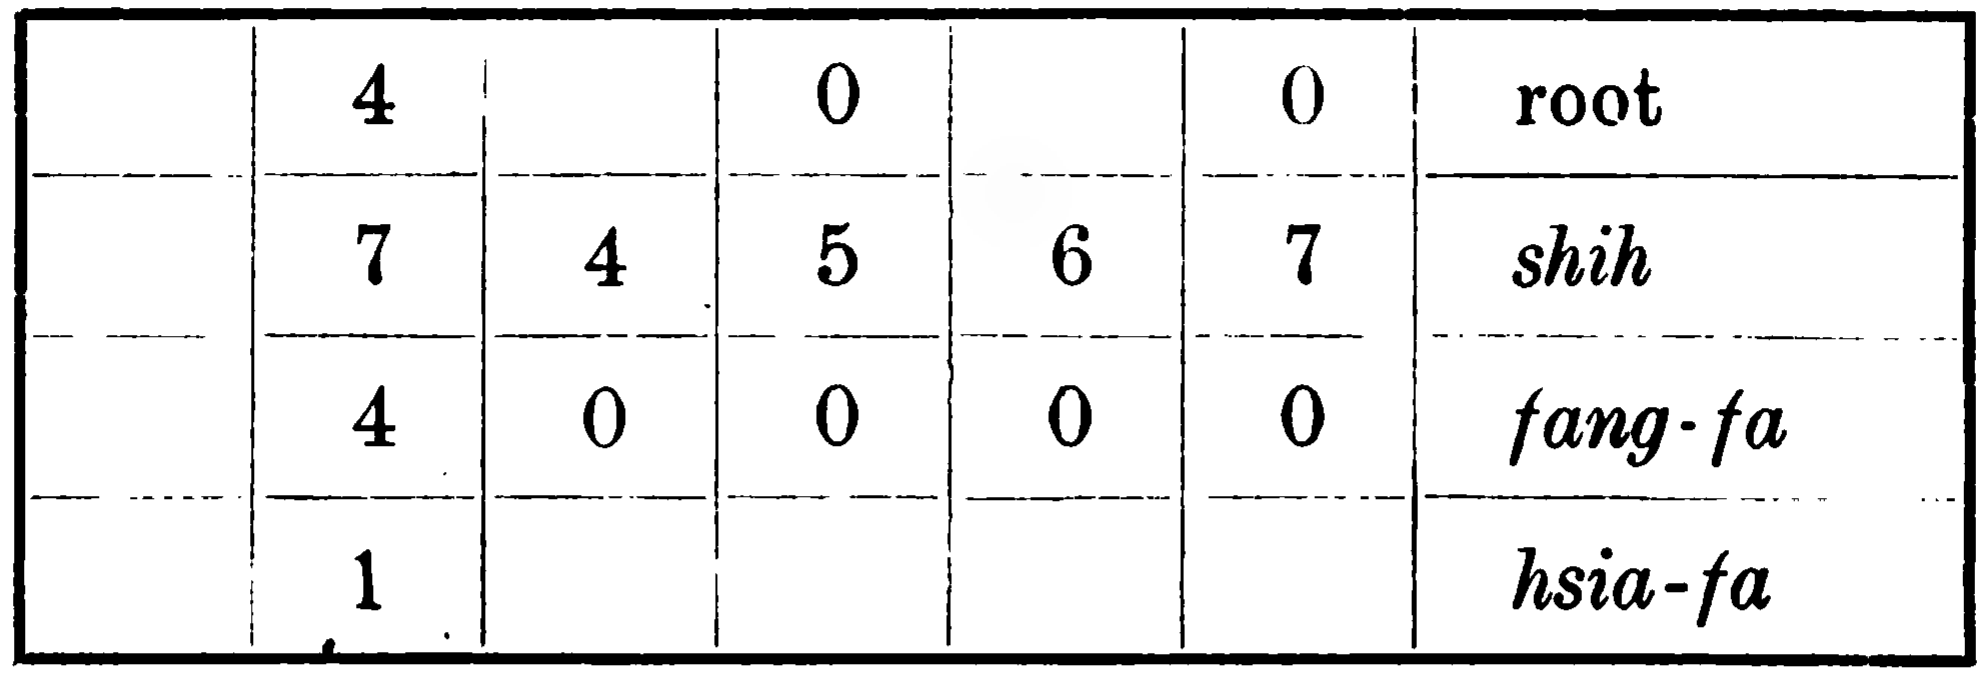
\includegraphics[width=.72\linewidth]{pdf044-sqrt-table-c.png}\end{center}

「減算が終わったら、\emph{fang-fa} を倍し、それを一列引き戻し、\emph{hsia-fa} を二列引き戻す。」すなわち、

\begin{center}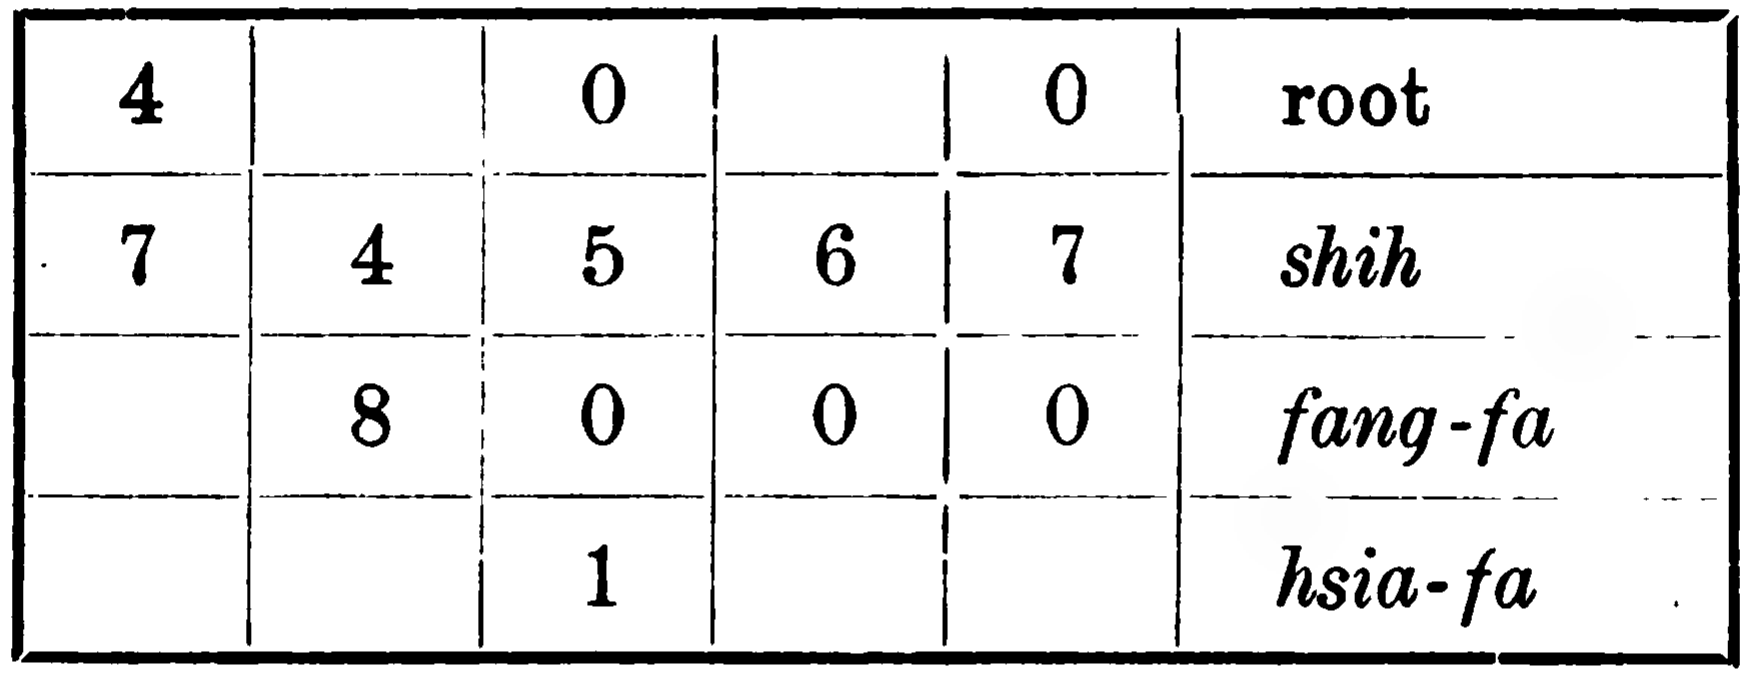
\includegraphics[width=.64\linewidth]{pdf044-sqrt-table-d.png}\end{center}

「さらに 80 を、前の桁の次の根として配列する。

「800 を \emph{fang-fa} の下、かつ \emph{hsia-fa} の上に添え、これを \emph{lien-fa} と名づける。

「\emph{fang-fa} と \emph{lien-fa} に根 80 を掛け、その積を \emph{shih} から引く。」すなわち、

\begin{center}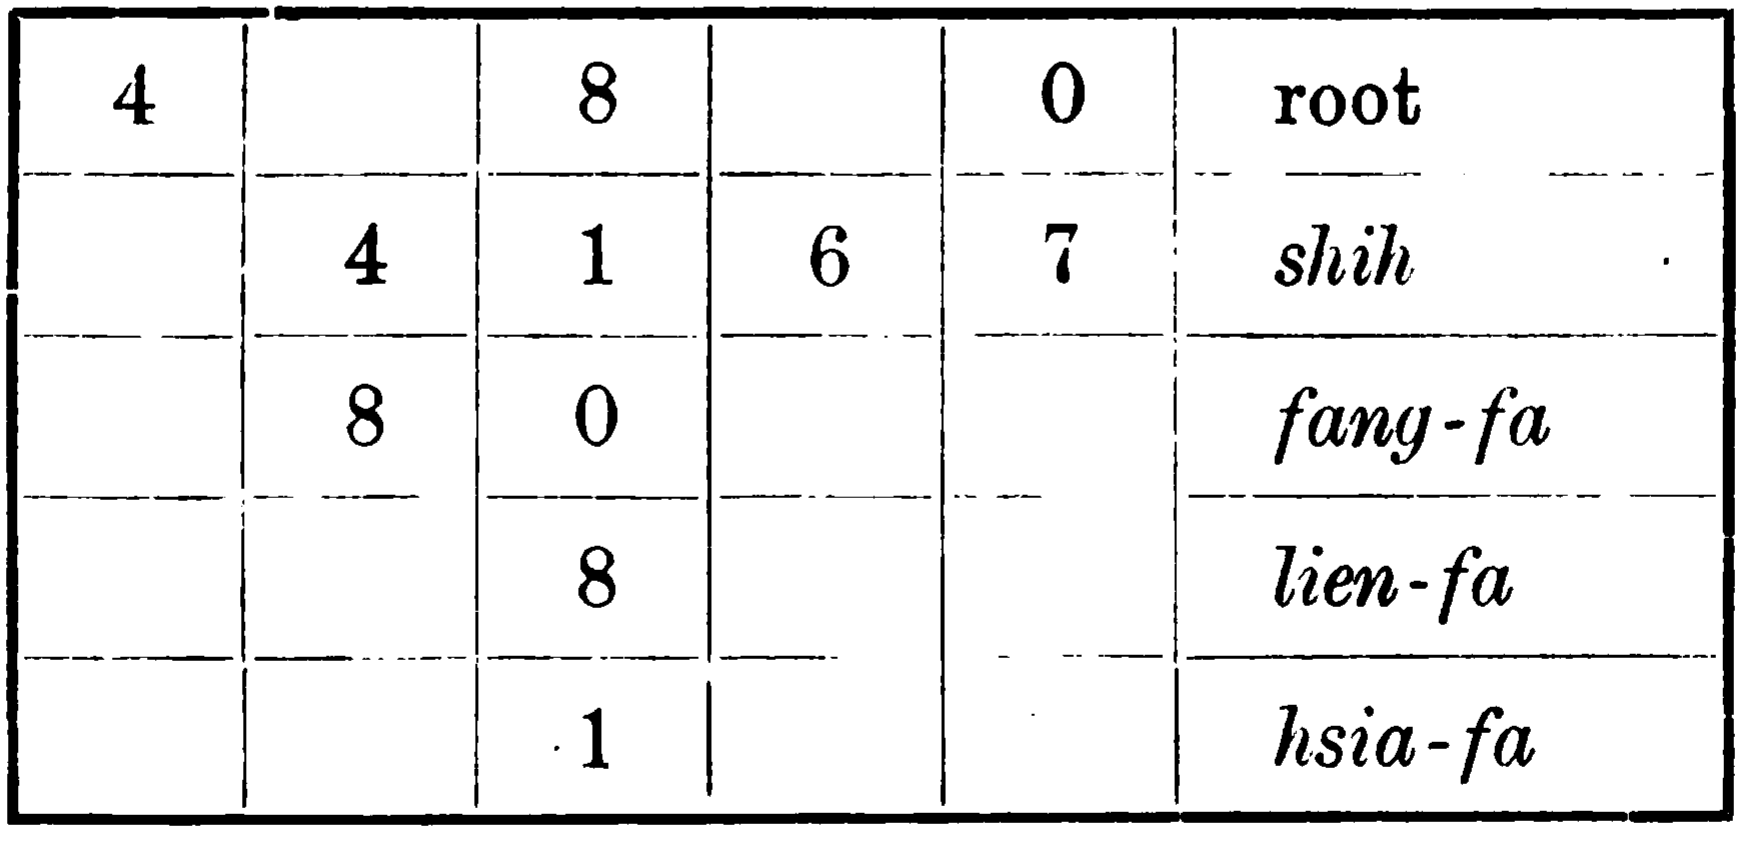
\includegraphics[width=.64\linewidth]{pdf044-sqrt-table-e.png}\end{center}

「これらの減算が終わったら、\emph{lien-fa} を倍して \emph{fang-fa} に加える。

「\emph{fang-fa} を一列、\emph{hsia-fa} を二列引き戻す。」
\scanfooter

\scanpage{0045}{第四章、印刷頁31}

ここで \emph{lien-fa} は取り除かれるものと理解される。こうして配列は次のようになる。

\begin{center}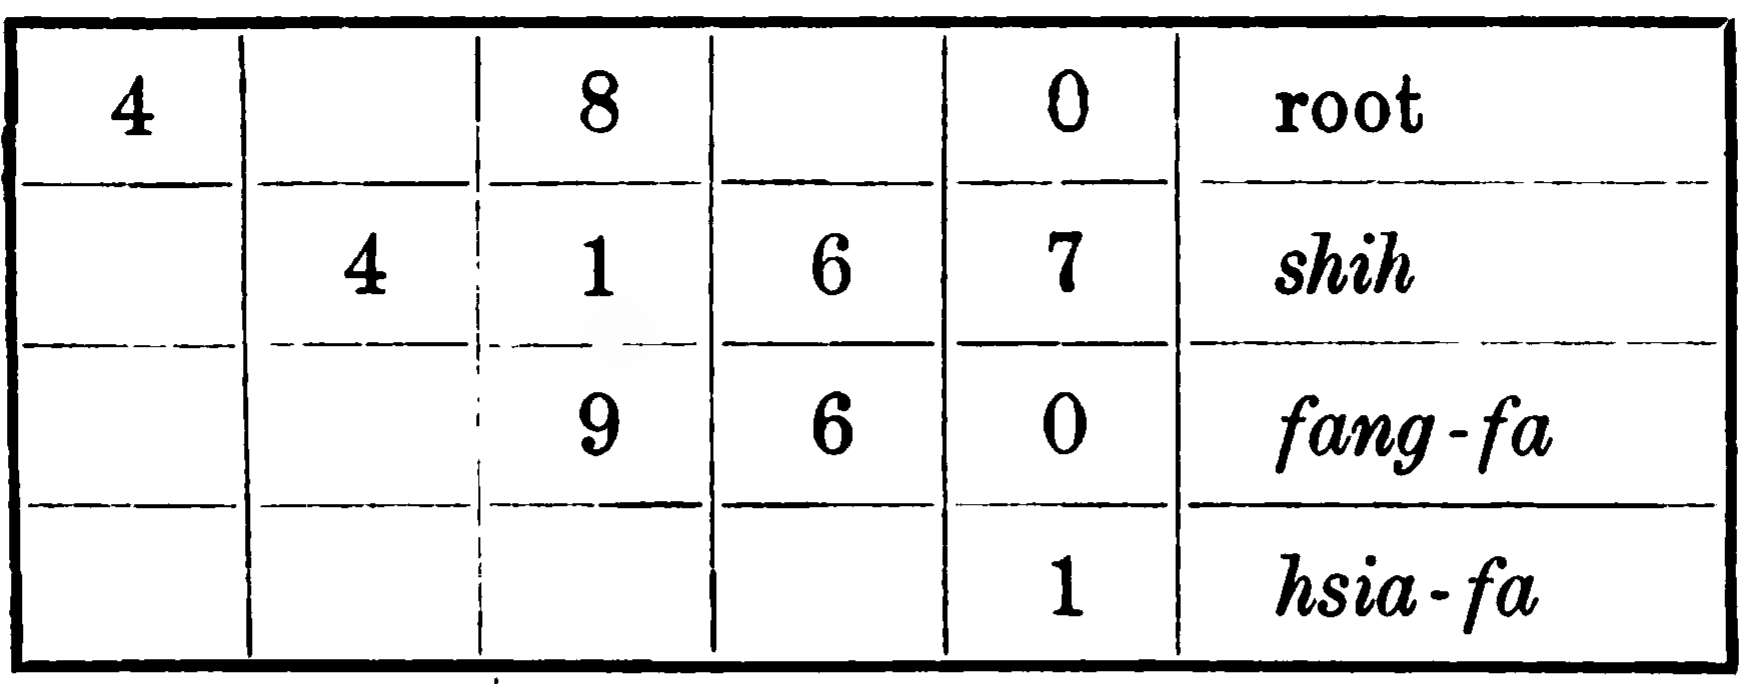
\includegraphics[width=.70\linewidth]{pdf045-sqrt-table-f.png}\end{center}

「さらに 4 を、前の根の次の列に配列する。

「4 を \emph{fang-fa} の下、かつ \emph{hsia-fa} の上に添え、これを \emph{yü-fa} と名づける。」\footnote{これは前の \emph{lien-fa} と同じであり、ただ別名で呼ばれているだけである。}

「\emph{fang}、\emph{lien}、および \emph{yü}\footnote{この一節はいくぶん奇妙に見えるかもしれないが、それは \emph{fang-fa} と \emph{yü-fa} とを根の 4 で掛けることを意味する。} を根 4 で掛け、その積を \emph{shih} から引く。」すなわち、

\begin{center}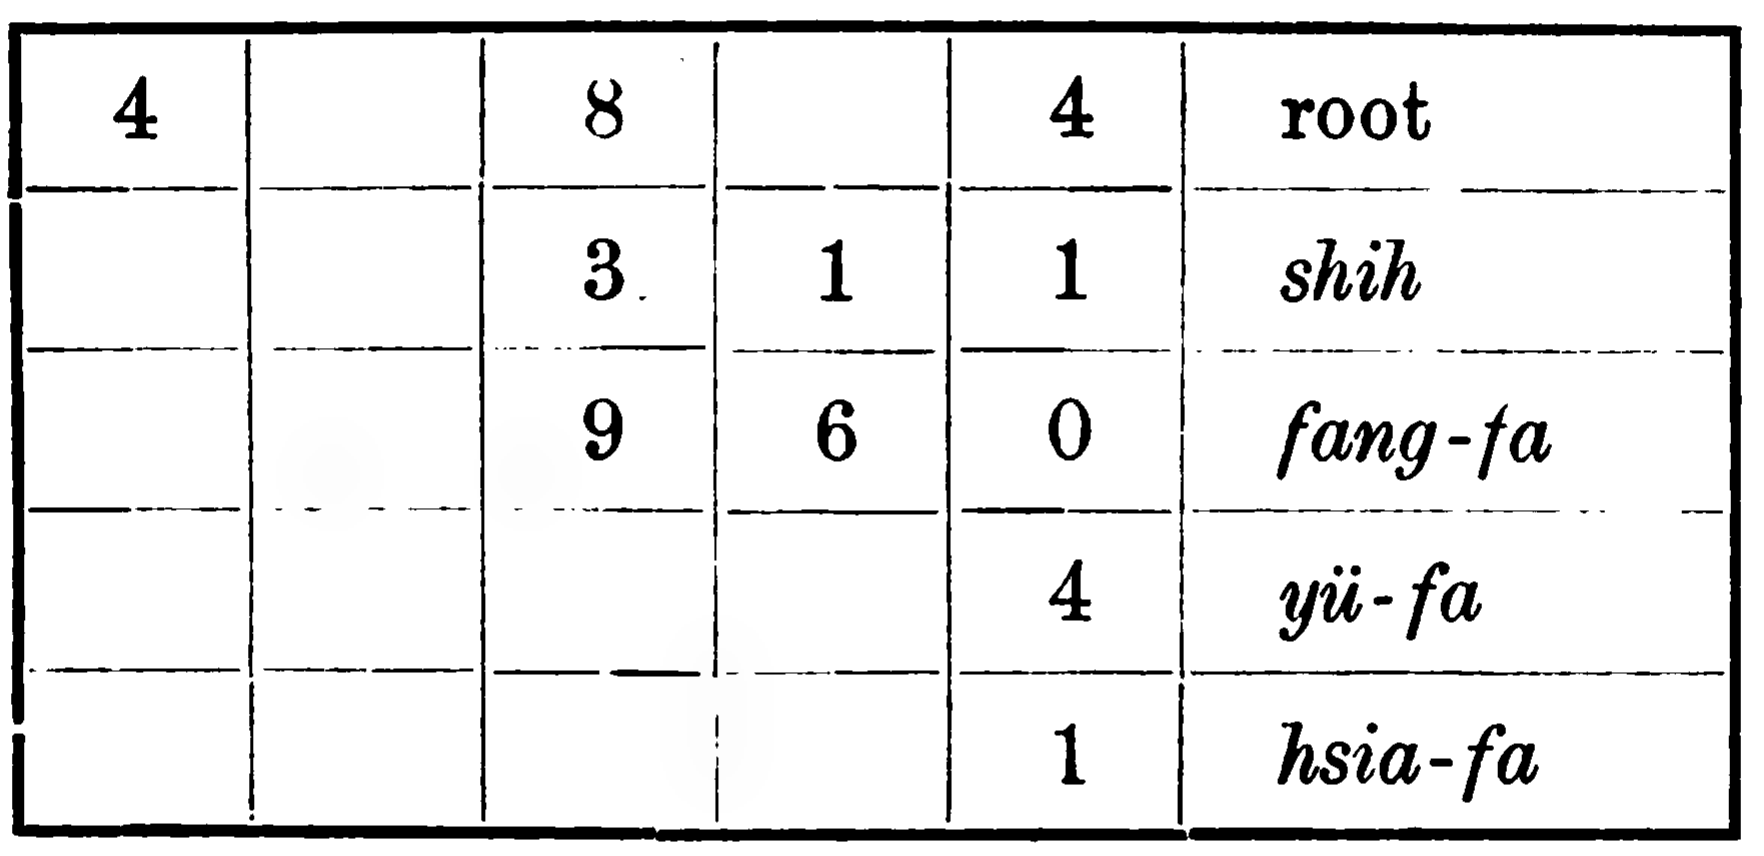
\includegraphics[width=.70\linewidth]{pdf045-sqrt-table-g.png}\end{center}

「これが終わったら、\emph{yü-fa} を倍して \emph{fang-fa} に加える。

「こうして上には根として 484 を得、\emph{hsia-fa}\footnote{これは以前と同じ意味ではない。} として 968 を得、余りは 311 となる。」

「したがって、（正方形の）一辺は $484\,\dfrac{311}{968}$ 歩である。」

この最後の段階は、「九章」においても採用されていたもので、古代中国のすべての数学者によって常に踏襲されたようである。

Sun-Tsŭ は立方根の場合を考察していない。

ここで Sun-Tsŭ の「算術経典」第三巻から、一つ二つの問題を掲げる。

「ある婦人が川で皿を洗っていたところ、水を監督する役人が彼女に尋ねた。『なぜここにこんなに多くの
\scanfooter

\scanpage{0046}{第一部、印刷頁32}

皿があるのか』――『家で饗宴が催されたからです』と婦人は答えた。そこで役人は客の人数を尋ねた。『何人の客がいたかは分かりません』と婦人はいった、『しかし二人ごとに飯の皿を一つ、三人ごとに汁の皿を一つ、四人ごとに肉の皿を一つ用い、皿は全部で六十五ありました。』」

「規則。65 枚の皿を配列し、12 を掛けると 780 を得る。これを 13 で割ると答を得る。」

「数が分からないものがある。3 で繰り返し割ると余りは 2、5 で割ると余りは 3、7 で割ると余りは 2 である。その数はいくつか。」

この問題は不定方程式
\[
3m_1+2=5m_2+3=7m_3=2
\]
に帰着し、その解は
\[
m_1=5\times7r+7,\qquad m_2=21r+4,\qquad m_3=3\times5r+3,
\]
ただし $r=0,1,2,3,\ldots$ である。

Sun-Tsŭ はこの問題を次のように解こうとする。

「3 で割った余りは 2 であるから 140 を取る。5 で割った余りは 3 であるから 63 を取る。7 で割った余りは 2 であるから 30 を取る。これらを合わせると 293 を得る。そこから 210 を引けば答を得る。」

このように Sun-Tsŭ は、その問題の一つの解だけで満足した。

Sun-Tsŭ はさらにいう。「一般に、3 で繰り返し割った余りが 1 であるときは 70 を取る。5 で繰り返し割った余りが 1 であるときは 21 を取る。7 で繰り返し割った余りが 1 であるときは 15 を取る。これらの数の和が 106 を超えるときは、答を得る前に 105 を引く。」

Sun-Tsŭ が扱ったすべての主題は、「九章算術」においてすでに与えられていたものだったが、不定解析の問題は、上に見たように Sun-Tsŭ において初めて現れた。

同時方程式
\[
2x+1y=96,\qquad 2x+3y=144
\]
に等しいものを解くにあたって、Sun-Tsŭ はこれらの方程式をそれぞれ他方の $x$ の係数で掛け、相互に引き算を行おうとする。彼がいかに形式に固執しているかを見よ。しかしまた、ここでは係数を互いに掛け合わせることによって、「九章」よりも一歩進んだ段階が得られていることも見よ。
\scanfooter

\scanpage{0047}{第四章、印刷頁33；第五章冒頭}

Sun-Tsŭ には最小公倍数を求める問題が見られる。それは次のものである。

「三人の姉妹がいる。長女は 5 日に一度、次女は 4 日に一度、末娘は 3 日に一度家に帰ってくる。三人全員が一緒に会うのは何日後か。」

答は 60 日である。

これを解くために Sun-Tsŭ は次の言葉で規則を与える。

「長女の 5 日、次女の 4 日、末娘の 3 日を右欄に配列する。これらそれぞれに対して、左欄に一を配列する。次に（右側の数を）交差して掛けると、それぞれが戻ってくる回数を得る。すなわち長女は 12 回、次女は 15 回、末娘は 20 回戻る。これらの数に、姉妹が一度戻ってくる日数を掛ければ、求める答が得られる。」

Sun-Tsŭ の「算術経典」における最後の問題は、占いに関するものである。すなわち、

「二十九歳の妊婦が、その年の第九月に子を産む予定である。その子は息子であるべきか、娘であるべきか。」

Sun-Tsŭ はこの問題に対して規則を与える。

「49 を取る。出産の月を加える。年齢を引く。いま残ったものから、天 1 を引き、地 2 を引き、人 3 を引き、四季 4 を引き、五行 5 を引き、六律 6 を引き、七星 7 を引き、八風 8 を引き、九州 9 を引く。そこで余りが奇数ならば子は男であり、偶数ならば女である。」

Yüan Yüan はその『伝記集成』において、この一問題を Sun-Tsŭ の原文ではなく後世の補入に帰したいと考えている。というのは、それが Sun-Tsŭ のような有能な著者にとってあまりに不似合いに見えるからである。

\begin{center}
CHAPTER 5.\par
\medskip
THE HAI-TAO SUAN-CHING OR THE SEA-ISLAND\par
ARITHMETICAL CLASSIC.\par
\medskip
第五章　\emph{Hai-tao Suan-ching}、すなわち海島算術経典。
\phantomsection\addcontentsline{toc}{subsection}{第5章　Hai-tao Suan-ching、すなわち海島算術経典}
\end{center}

\emph{Hai-tao Suan-ching}、すなわち字義どおりには「海島算術経典」は、三国の戦乱期に魏王国に属していた Liu Hui によって著された論著であった。

\scanfooter

\scanpage{0048}{第一部、印刷頁34}

三国時代である。\footnote{三国の時代は、紀元三世紀初めの後漢崩壊とともに始まり、半世紀続いた。三国とは、北の魏、南の呉、西の蜀である。魏王国は二六五年、晋王朝が勢力を得たとき滅ぼされた。}「海島算術経典」という題名は、もともと著者自身によって付けられたものではなかった。すでに述べたように、Liu Hui は「九章算術」に注釈を付け、\emph{Chung-ch'a} という標題の下に分類したいくつかの問題の解法を処理し、九章の最後である \emph{Kou-ku} 章の次にそれらを加えた。しかし Liu の追加部分は「九章」の本文を構成し得ず、やがて別個に考えられる運命となり、今日輝かしく掲げている題名を取るようになった。この題名は、この書の第一問題が離れたところから島を測量することに関するために起こったもので、おそらく七世紀に興った唐王朝の初めから用いられたのであろう。

Liu Hui の著作の正本は残っていない。それは明政府によって永楽年間（一四〇三--一四二四）に編纂された『\emph{Yung-lo Tai-tien}』という題名をもつ写本群の中に保存されていたにすぎない。われわれが現在所有する「海島算術経典」は、先に述べた大集成の中から、帝国の司書であり数学者であった Tai Chêng が一七七五年に採録したものである。この書には、七世紀中頃に活躍した Li Ch'un-fêng の注釈が付されている。

Liu Hui の生涯についてはほとんど何も知られていない。ただし、『\emph{Chin Shu}』、すなわち「晋書」から分かるように、彼は魏王国の Ch'ên-liu-Wang の治世下、紀元二六三年に「九章算術」への注釈を書いた。Liu の年代についていくつか異なる意見があるとしても、「晋の記録」における記述が最も信頼すべきものだと信じざるを得ない。

「海島算術経典」の第一問題は次のものである。

「測るべき海島がある。ともに高さ 30 尺（$a$）の二本の竿を、互いに 1000 歩（$b$）離して立て、後ろの竿が島および他方の竿と同一直線上に来るようにする。人が近い方の竿から 123 歩（$c$）後退し、目を地面に接するようにして見ようとすると、島の頂上はその竿の端を通してちょうど見える。島の峰の頂もまた、
\scanfooter

\scanpage{0049}{第五章、印刷頁35}

その後ろの竿の端と一直線に見えるが、それはその竿から 127 歩（$d$）後退した地点で、目を地面に接して見たときである。島の高さと距離を知ることが求められる。」

この問題の解法として与えられる規則は次のように述べられている。

「規則。竿の高さに竿の間の距離を掛け、（その積を）被除数とする。そして、竿から後退した距離の差を除数として割り算を行う。商に竿の高さを加えれば、島の高さを得る。

「近い方の竿から島までの距離を求めるには、その竿から後退した距離に二本の竿の間の距離を掛け、その積を竿から後退した距離の差で割る。その商が求める距離を与える。」

この規則は次の公式に等しい。
\[
(\text{高さ})=a+\frac{ab}{d-c};\qquad (\text{距離})=\frac{cb}{d-c}.
\]

Liu Hui がこれらの式をどのように得たかは知られていないが、それらが二つの比例式
\[
\frac{x}{x+c}=\frac{a}{c},\qquad \text{および}\qquad \frac{x}{x+b+d}=\frac{a}{d}
\]
またはそれらと同等なものから導かれたと考えることは、おそらくありそうにないことではない。

語 \emph{chung-ch'a} は、われわれの見解との一致を示すように思われる。この語は本来、「九章」の直角三角形の章に見られる考察の二重または反復適用、すなわち比例の二重適用を意味することを意図したものであった。

Liu Hui の第二問題は次のとおりである。

「丘の上に松の木が生えており、その高さは分からない。高さ 20 尺（$a$）の二本の竿を、下の平地に相互に 50 歩（$b$）離して、木と一直線になるように立てる。木の頂と前の竿の端は、竿の後ろ 7 歩 4 尺（$c$）の地上の一点と一直線をなし、この点で木の根元は竿の上端に 2.8 尺（$e$）として測られる。木の頂はまた、後ろの竿の端およびその竿の後ろ 8 歩 5 尺（$d$）の地上の一点と一直線をなす。松の木の高さと、丘から（前の）竿までの距離を知ることが求められる。」
\scanfooter

\scanpage{0050}{第一部、印刷頁36；第五章終わり}

この問題を解くことを意図した規則は、次の公式へ導く。
\[
(\text{高さ})=\frac{eb}{d-c}+e;\qquad (\text{距離})=\frac{bc}{d-c}.
\]

第三問題は次のものである。

「南に、大きさの分からない正方形の町が見える。彼は東西方向に 60 尺（$a$）離して二本の竿を立て、目の高さに紐でそれらを結び、東の竿が町の南東隅および北東隅と一直線になるようにする。

\begin{center}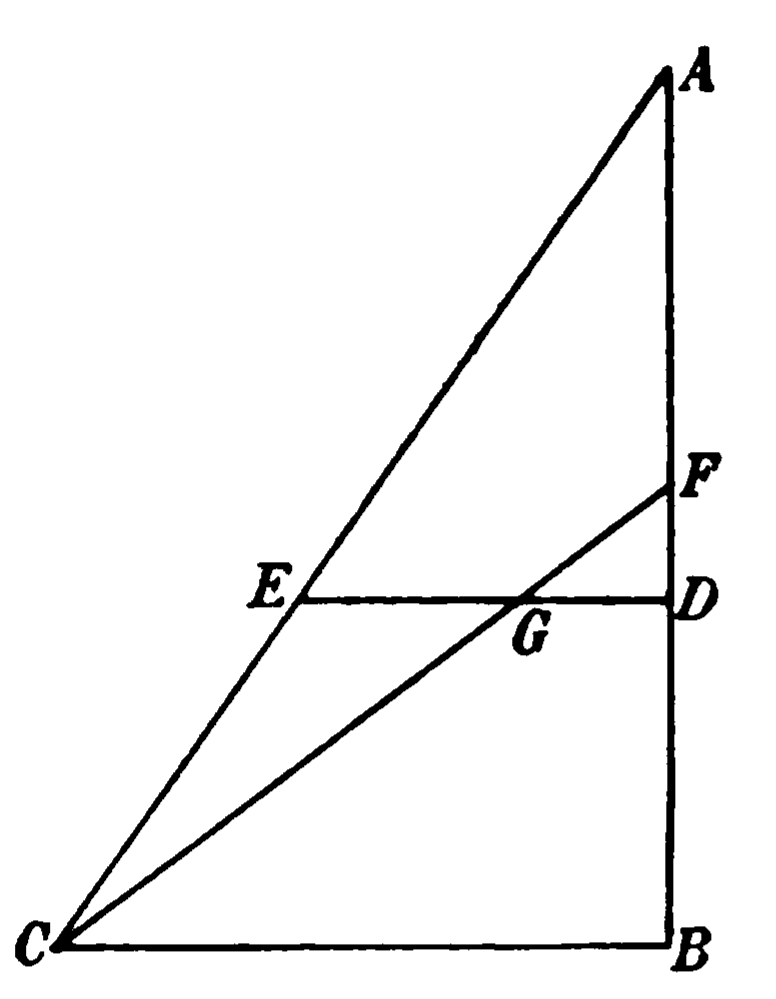
\includegraphics[width=.28\linewidth]{pdf050-square-town-diagram.png}\end{center}

彼は東の竿の北へ 5 歩（$b$）行き、東端から $22\cdot6\frac{1}{2}$ 尺（$c$）の紐上の一点を通して町の北西隅を観測する。さらに竿から北へ 13 歩 2 尺（$d$）後退すると、観測者は町の北西隅がちょうど西の竿と一直線になるのを見る。そのとき、町の一辺と竿から町までの距離はいくらか。」

この問題は、（図を見よ）$DE=a$, $DF=b$, $DG=c$, $DA=d$ によって $CB=x$ および $BD=y$ の長さを求めることと同じである。［図では $B$ が直角で、$DE$ は $BC$ に平行に引かれている。］

答の公式は次と同等な形で与えられる。
\[
x=\frac{(d-b)c}{\dfrac{cd}{a}-b},\qquad
 y=\frac{\left(d-\dfrac{cd}{a}\right)b}{\dfrac{cd}{a}-b}.
\]

Liu Hui はその「算術経典」において、これに類似する六つの問題を、解法規則とともにさらに与えている。

Liu Hui がこれらの複雑な問題を研究していることは、彼が何らかの代数的操作の方法を知っていたことを物語るように思われる。さらに「九章」のいくつかの部分の内容を考えるならば、中国の代数の誕生を、一般に中国代数が生まれたと信じられている十三世紀の Ch'in Chiu-shao と Li Yeh の出現の時代よりも、はるかに早い中国史の比較的初期に帰さざるを得ない。したがってわれわれは、Liu Hui によるこれらの複雑な問題の考察に重きを置く。それは三世紀に行われたものであり、後に少し考察しなければならない天元術の代数の黎明よりも、まる一千年前のことであった。
\scanfooter

\scanpage{0051}{第六章、印刷頁37}
\begin{center}
CHAPTER 6.\par
\medskip
THE WU-T'SAO SUAN-CHING AND THE WORKS OF HSIA-HOU\par
YANG, CHANG CH'IU-CHIEN AND CHÊN LUAN.\par
\medskip
第六章　\emph{Wu-t'sao Suan-ching} および Hsia-hou Yang、Chang Ch'iu-chien、Chên Luan の著作。
\phantomsection\addcontentsline{toc}{subsection}{第6章　Wu-t'sao Suan-ching および Hsia-hou Yang、Chang Ch'iu-chien、Chên Luan の著作}
\end{center}

次に記述すべきものは、唐政府が文官選抜の広大な試験制度における教科書として採用した算術経典であって、これまで概観したもの以外でなお現存するものである。すなわち \emph{Wu-t'sao Suan-ching} と、Hsia-hou Yang、Chang Ch'iu-chien、Chên Luan の著作を意味する。

これらのうち \emph{Wu-t'sao Suan-ching} の著者は知られていない。この題名は、おそらくこの書が五つの異なる標題の下に扱われる五巻または五章を含むために与えられたのであろう。その成立年代もまた不明である。同様に、二人の数学者 Hsia-hou Yang と Chang Ch'iu-chien の年代もすべて失われている。しかし Hsia-hou はその著作の序で次のように述べている。

「しかし算術は Fu-hi の時代から曙を迎え、黄帝\footnote{黄帝は紀元前二十七世紀に属した。} は三数を整え、十度\footnote{これらは算術的考察における何らかのものと理解される。} を作り、Li-Shou はそれによって『九章』を作った。…… \emph{Wu-t'sao} と Sun-Tsŭ の後には、さまざまな算術書が現れ、Chên Luan と Liu Hui はこれらの書に詳しい注釈を書いた。……」

Chang Ch'iu-chien は、その著作の序において、Hsia-hou Yang および Sun-Tsŭ の解法のいくつかを改めると明言しており、彼は実際にその書の本文でそれを行っている。

したがって、Sun-Tsŭ と \emph{Wu-t'sao Suan-ching} は最も早い時代、確かに前漢または後漢の時代に属し、Hsia-hou と Chang の著作はそれより後の時代に現れたものと見られる。しかし、Chang の「算術経典」が Chên Luan によって注釈されたという事実を考え、しかもその Chên の注釈は今では失われていること、また Hsia-hou が Sun-Tsŭ と \emph{Wu-t'sao Suan-ching} の著作に対する Liu Hui と Chên Luan の注釈に言及していることを考えるならば、二人の著者 Hsia-hou と Chang は疑いなく Chên Luan と同時代人であったと結論しなければならない。さらに Yüan Yüan\footnote{Yüan の『\emph{Biographical Notices}』、第十一巻。} によれば、Chên Luan は Hsia-hou Yang の「算術経典」にも注釈を書いた。
\scanfooter

\scanpage{0052}{第一部、印刷頁38}

Hsia-hou はその著作本文で、体積の度量衡の標準が四二五年に再建され、さらに五三五年に Chên Luan によって再建されたと書いている。Chên Luan が六世紀後半に周の皇帝 Wu-Ti に大臣として仕えたことはよく知られている。彼は迫害に抗して仏教を支持することに非常に熱心であった。Chên Luan の \emph{Wu-ching Suan-shu} は周王朝の治世下の著作であり、彼自身がそこに、その王朝、すなわち五五七年に成立し五八一年に滅んだ王朝に属すると署名しているからである。

したがって、いま考察中の数学書は、\emph{Wu-t'sao} を除いて、安全に六世紀のものといえる。

われわれはまず、これらの著作のうち最古のもの、すなわち \emph{Wu-t'sao Suan-ching} を記述しよう。

この書には、解法の規則が奇妙で分かりにくく見える問題がいくつかある。後世の学者はこれらを誤りとみなしている。

たとえば「鼓形」の田の面積は、その形が、おそらく二つの合同な等脚台形から成り、その二つの等しい底辺、すなわち大きい方または小さい方を一致させたものであるが、三つの底辺の和の三分の一と高さとの積に等しいとされる。

円分の面積は、その弦の半分と高さとを掛けることによって計算される。その結果は「九章算術」に見られるものよりも粗い。

「四辺形の田があり、その東側は 35 歩、西側は 45 歩、南側は 25 歩、北側は 15 歩である。この田の面積を求めることが要求される。」

この問題は次の規則で解かれる。

「東側と西側を加えると 80 歩となり、これを半分にすれば 40 歩を得る。さらに南側と北側を加えると 40 歩となり、これを半分にすれば 20 歩を得る。二つを掛けると積 800（平方）歩となり、……これが求める答である。」

これは、四辺形の面積を、相対する二組の辺の和の積の四分の一と呼んでいるだけである。その誤りは明らかである。

伏した月の形をした田（おそらく二つの円弧によって囲まれた月形）は、その長さの半分（共通弦）とその直径（おそらく二つの弧の間で切り取られる共通矢の部分を意味したのであろう）との積によって測られるとされる。
\scanfooter

\scanpage{0053}{第六章、印刷頁39}

以上はすべて \emph{Wu-t'sao Suan-ching} 第一巻に見られる。この書のすべての問題は、乗法と除法の適用によって解かれている。

\emph{Hsia-hou Yang Suan-ching}、すなわち「Hsia-hou Yang 算術経典」は三巻から成る。この著作は六世紀中頃または後半に属する。

Hsia-hou は、数の配列、ならびに乗法と除法について、Sun-Tsŭ と同じことを述べている。書中のある段階では著者は \emph{Wu-t'sao Suan-ching} に従い、別の段階では古い「九章」に基づいて考察している。Hsia-hou は、二つの合同な台形から成る図形および四辺形の面積規則において、\emph{Wu-t'sao Suan-ching} と同じ誤りを犯している。しかし円分の面積については「九章」に従い、\emph{Wu-t'sao Suan-ching} には従っていない。

Hsia-hou は円の面積について三つの公式を与えている。

Hsia-hou は平方根の抽出を Sun-Tsŭ とまったく同じ仕方で記述している。ただし、Sun-Tsŭ が行い「九章」にも示されているように、操作後の余りを得られた平方根の分数部分として与えることはしない。彼はただ、そのような余りが操作後に残ることを付け加えるだけである。

Hsia-hou Yang が考察した問題は、すべて乗法と除法の適用および単純な百分法に制限されている。ただし、体積の測定等に関するいくつかのものを除く。

\emph{Chang Ch'iu-chien Suan-ching}、すなわち「Chang Ch'iu-chien 算術経典」は、おそらく六世紀後半に属し、三巻または三章から成る。書の一部は現在欠けており、失われている。この著作は、他の古い著作とともに、一〇八四年に宋政府が作った版を通して保存された。そこには Liu Hs'iao-sun による規則の詳しい説明が補われ、七世紀には Li Ch'un-fêng によって注釈された。

Chang はその著作の序で、「算術を学ぶにあたって、われわれは乗法と除法の困難に悩まされるのではなく、分数を考える困難に悩まされる」と述べている。彼はこのように分数の処理を重視している。

分数による除法の問題がこの書に見られる。そのうち二つがあり、一つは次のものである。

「$27\dfrac{3}{5}$ で $1768\dfrac{4}{7}$ を割り、何が得られるかを求める。」
\scanfooter

\scanpage{0054}{第一部、印刷頁40}

答は $64\dfrac{38}{483}$ と与えられるが、Chang の本文にはその操作の規則は与えられておらず、それは Liu Hs'iao-sun の説明によって補われている。

二つの問題のうち他方は次のものである。

「$58\dfrac{1}{2}$ で $6587\dfrac{2}{3}+\dfrac{3}{4}$ を割り、答を求める。」

この問題には次のような規則が与えられている。

「6587 を上に配列する。これとは別に、その下に、分母 3 を右に、分子 2 を左に配列する。さらに分母 4 を 3 の下の右に、分子 3 をその左に配列する。次に交差して掛けると、分母として 12、分子として 17 を得る\footnote{この簡潔な叙述は、二つの分数の加法を示すものと理解すべきである。}。分子を分母で割ると、商として 1 を得、これを上の数に加えるべきであり、これによって 6588 となる。これに分母 12 を掛け、そこに分子 5 を加えて 79 061 を得る。さらにこの数に、除数の分母 2 を掛けると 158 122 を得る。さらに除数 58 を下に配列し、2 を掛け、分子 1 を加えて 117 を得る。さらに被除数の分母 12 をこれに掛けると 1404 を得る。これを除数として除法を行うと 112 を得、除数と余りはともに半分にされ、分数部分は $\dfrac{437}{702}$ と得られる。」

この規則から、分数 $\dfrac{a}{b}$ を別の分数 $\dfrac{c}{d}$ で割ることは、第三の分数 $\dfrac{ad}{bc}$ を作ることによって行われたことが分かる。これから、古い中国人は、分数で割ることが逆分数を掛けることに等しいことを知っていたと推測できる。もしこの定理が明示的には述べられていないとしても、結果はまったく同じである。この定理はヨーロッパでは十六世紀になって初めて得られたが、ヒンドゥーの Mahavirakarya は九世紀にこれを知っていた。\footnote{D. E. Smith, \emph{Bibliotheca Mathematica}, 1909.}

Chang Ch'iu-chien はさらに、「海島算術経典」に見られるような問題を扱っている。彼はまた、百分法による配分、過不足、連立方程式、および \emph{kou-ku}、すなわち直角三角形に関する問題も与えている。

Chang は他の古い中国の著作とは異なり、等差数列を一般的な仕方で考えている。すなわち、
\scanfooter

\scanpage{0055}{第六章、印刷頁41}

「ある婦人がいて、初日に 5 尺を織り、日ごとにその織る量が減って、最後の日には 1 尺を織る。彼女が 30 日織ったと仮定して、その織った総量を知ることが求められる。」

この問題に対して Chang は次の規則を与える。

「初日と最終日に織った量を加え、その和の半分を取る。次にそれに織った日数を掛ければ、答を得る。」

これは、等差数列の和を、初項と末項の和の半分と項数との積によって与えるものである。

もう一つの問題は次のものである。

「日ごとに織る量が増す織女がいる。彼女は初日に 5 尺を織り、一か月に 9 \emph{p'i} と 30 尺を織る。日ごとの増加量を求めることが要求される。」

ここで著者は解法規則を付け加える。

「織った尺数を配列し、それを一か月の日数で割る。得られた商を二倍し、そこから初日に織った尺数の二倍を引く。その結果を被除数とする。そして一か月の日数から一日を減じた数でこれを割る。その商が答である。」

等差数列の初項、公差、項数、和をそれぞれ $a$, $x$, $r$, $k$ で表すならば、上の規則は公式 $x=\left(\dfrac{2k}{r}-2a\right)\div(r-1)$ に等しく、これは正しい。

Chang は、幾何図形に関係しない比例の問題を考察している。次はその一つである。

「馬を盗んだ男が、その背に乗って逃げた。彼が 37 中国里（$a$）進んだとき、持ち主が盗難に気づき、145 里（$b$）追跡した。しかし追いつけず、そこで引き返した。彼が引き返した時、盗人は 23 里（$c$）先を進んでいた。もし彼が引き返さずに追跡を続けていたならば、さらに何里で追いついただろうか。」

この問題は、次の公式と等しい規則によって解かれる。
\[
c\times b\div(a-c).
\]

Chang はまた複比例の問題を解いている。

「7 人（$a$）が 9 日（$c$）で $12\frac{1}{2}$ 張（$b$）の弓を作るならば、17 人（$d$）が 15 張（$e$）の弓を作るには何日を要するか。」
\scanfooter

\scanpage{0056}{第一部、印刷頁42}

必要な日数は $=(e\times c\times a)\div(d\times b)$ と与えられる。

実際のところ、著者がわれわれが現在試みるような通常の過程を適用したのかどうかは確かではない。

Chang の著作には等比数列に関する問題がある。

「ある馬は毎日その速さを半分にしながら、7 日で 700 里を走る。その各日の道程はいくらか。」

Chang はこの問題を次の公式に従って解いている。
\[
700\times(\text{各日の率})\div(64+32+16+8+4+2+1),
\]
ここで第一日の率は 64 と取られている。また彼は、手元の等比数列の和に対して一般公式を適用していない。これはおそらく古代中国人には知られていなかったのであろう。

与えられた角錐から、与えられた断面によって切り取られた正四角錐の高さは、Chang によって次のように述べられている。
\[
(\text{新しい高さ})=\frac{(\text{断面の辺})\times(\text{高さ})}{(\text{底面の辺})}.
\]

これは、高さが断面の辺に比例するという定理を含んでいる。

平方根を抽出するにあたって、Chang は Sun-Tsŭ および Hsia-hou Yang と同じ道筋に従う。意味において非常に奇妙な追加分数は、この有名な著者の場合にも現れる。

立方根の抽出もまた考察されている。

弦が $68\dfrac{3}{5}$、面積が $514\dfrac{32}{45}$ である円分の高さを求める問題において、Chang Ch'iu-chien は答を $12\dfrac{2}{3}$ と与える。彼は二次方程式を適用したように思われる。ただし、その規則の最後の部分は欠けている。というのは、彼は面積を \emph{shih}、すなわち定数項、弦を \emph{tsung}、すなわち一次の項と二度述べ、その後に続くべき語が欠けているからである。

この見解は、円分の面積について得られる式と一致している。
\[
(\text{面積})=\frac{1}{2}\{(\text{高さ})\times(\text{弦})+(\text{高さ})^2\}.
\]

Chang は二次方程式に適用される別の問題も考察している。

「高さ 120 尺（$h$）の円錐台があり、これに米がこれこれ（$r$）入っている。上底の円周が 15 尺（$c$）であるならば、下底の円周はいくらか。」
\scanfooter

\scanpage{0057}{第六章、印刷頁43}

この問題は次の方程式によって解かれるものと示されている。
\[
x^2+cx+\frac{r}{h}\times 36-c^2=0,
\]
ここで $r$ は平方尺で表した米の量である。あるいは、むしろ根を抽出する操作に、添えたような配列を適用するものである。

\begin{center}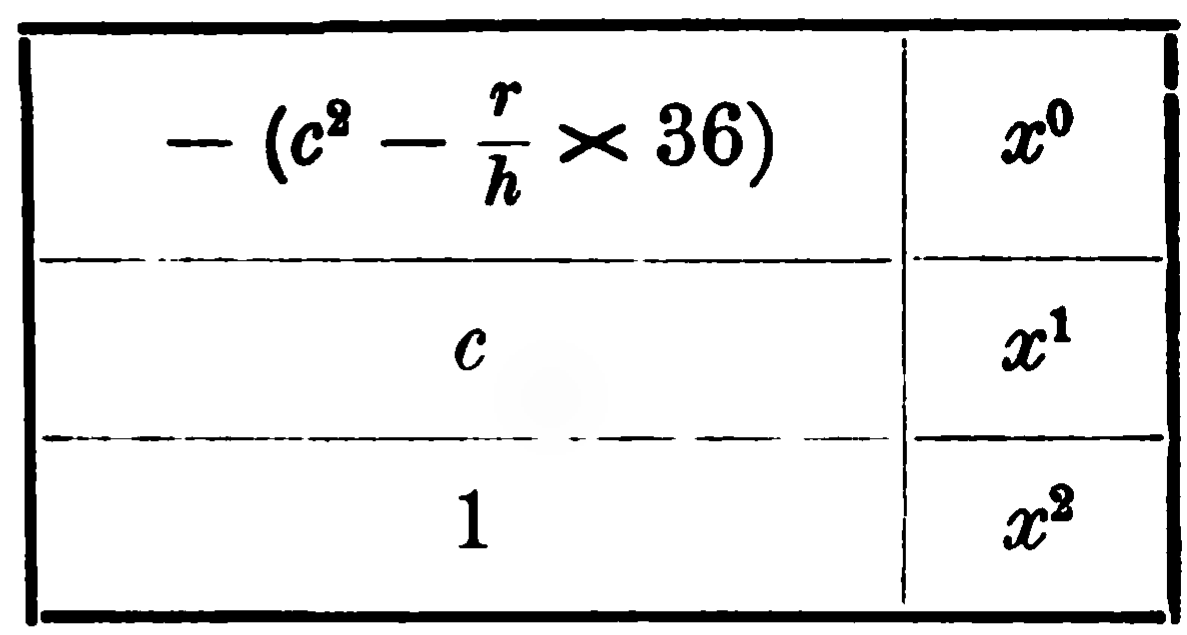
\includegraphics[width=.48\linewidth]{pdf057-quadratic-arrangement.png}\end{center}

Chang の著作における一問題は、「百鶏問題」として知られるようになったもので、注目すべきである。というのは、それに対して異なる組の解が採用されるからである。問題は次のとおりである。

「雄鶏は 5 銭、雌鶏は 3 銭、雛 3 羽は 1 銭である。そこで 100 銭でそれらを 100 羽買うならば、それぞれの数はいくらか。」

これは次の不定方程式系に等しい。
\[
x+y+z=100,\qquad \text{かつ}\qquad 5x+3y+\frac{1}{3}z=100.
\]

Chang は答を次のように与える。
\[
\begin{array}{rcl}
(1)& 4\ \text{羽の雄鶏},&18\ \text{羽の雌鶏および }78\ \text{羽の雛};\\
(2)& 8\ `` ,&11\ ``\quad ``\quad 81\ `` ;\\
(3)&12\ `` ,& 4\ ``\quad ``\quad 84\ `` .
\end{array}
\]

この解法に対する Chang の規則は、きわめて粗く次のように述べられている。

「雄鶏は毎回 4 ずつ増え、雌鶏は毎回 7 ずつ減り、雛は毎回 3 ずつ増える。こうして答を得る。」

ここで Tai Chêng はその校訂版において、この規則はほとんど理解し難いが、注釈者 Chên Luan と Li Ch'un-fêng でさえその説明を明らかにしたとは知られていない、と付け加えている。Tai はさらに、その解法の規則として、十三世紀以前の宋代に生きた Shieh Ch'a-wei によって得られたものを加えている。この解法もまた一般的な種類のものではない。特定の解を得るために、彼はただ、雛が $\dfrac{1}{3}$ 銭なので、雄鶏と雌鶏は 3 で掛けられ、その数が加えられるべきであるとして、価格 100 銭を $3+3+3=9$ で割り、雌鶏の数を導けと示唆するだけである。すると余りを除数 9 から引いたものが雄鶏の数を与える。

同様の問題は、漢代に属した Hsü Yüeh によって書かれた \emph{Su-shu Chi-i} に対する Chên Luan の注釈にも見られる。
\scanfooter

\scanpage{0058}{第一部、印刷頁44}

Hsü Yüeh は、二世紀中頃に生きた名声ある政治家であり天文学者であった Liu Hung の弟子であったと信じられている。二八五年に編纂された『\emph{San-kuo Chih}』、すなわち「三国志」によれば、呉王国の大臣となり二四三年に没した天文学者 Han Chai は、Liu Hung の暦法理論を Hsü Yüeh から学んだ。これらの考察は、Hsü の生涯をおよそ二〇〇年頃に定める。注釈者 Chên Luan は、すでに述べたように六世紀に属した。

Chên が Hsü の著作への注釈で解く問題は次のように述べられる。「雄鶏が 5 銭、雌鶏が 4 銭、雛 4 羽が 1 銭であるとき、100 銭で雄鶏・雌鶏・雛を合わせて 100 羽にするには、それぞれ何羽買えるか。」

Chên はその答を雄鶏 15 羽、雌鶏 1 羽、雛 84 羽としている。

雄鶏が 4 銭、雌鶏が 3 銭、雛 3 羽が 1 銭であるならば、Chên が解くように、答は雄鶏 8 羽、雌鶏 14 羽、雛 78 羽となる。

Hsü Yüeh はその本文で「できるだけ計算によって測定することを避け、心の判断によってなされるようにせよ」と述べている。ここで Chên Luan は、この文の意味を、いくつかの問題は算木によるよりも直接の考察によってよりよく答えられる、ということだと説明する。そこで彼は幾何学的構成を適用する。

「幅の分からない大きな川がある。算木を用いずにそれを測ることが求められる。」

ここで川は西から東へ流れているものと仮定される。

この問題の解法のために、Chên Luan は川の北側に三本の竿を北から南へ一直線に、互いに 10 尺離して立てる。そして中央の竿から、南側の竿上の二点を通して川の両岸を見る。その二点はそれに応じて印を付けられる。次に彼はこれらの印の高さを北側の竿に移し、中央の竿からそれらを通して地上の二点を見る。その二点間の距離が、測るべき川幅を与える。

長い杖の長さを測るには、Chên Luan は既知の長さの竿を立て、その影で杖の影を測る。

深い井戸の深さを知るために、Chên はたとえば長さ 10 尺の棒をその中に投げ入れ、手を伸ばして持った別の棒の端を通してそれを見る。それから人に、長さ 10 尺の棒を持ってさらに遠くへ遠くへと後退させ、
\scanfooter

\scanpage{0059}{第六章、印刷頁45；章終わり}

その棒が手に持った棒の印に対応して見えるようにする。そのとき、その人が歩いた距離が井戸の深さを表す。

Yüan Yüan\footnote{Yüan の『\emph{Biographical Notices}』、第十一巻。} によれば、Chên Luan は周の皇帝 Wu-Ti の治世に暦法体系を作った。彼はまた、\emph{Chou-pei}、Chang Ch'iu-chien の「算術経典」、Tun Ch'üan の \emph{San-têng-shu}、Hsia-hou Yang の「算術経典」、「九章算術」、\emph{Wu-t'sao Suan-ching}、およびその他の暦法書に注釈を書いた。Chên Luan は数学および関連分野において学識ある人物であったばかりでなく、仏教の書物にも深く通じていた。彼は \emph{Wu-ching Suan-shu}、すなわち「五経算術」を書き、その中に経典、\emph{Yi-ching}、\emph{Shu-ching}、\emph{Shi-ching}、\emph{Lun-i} などに言及されたさまざまな問題を盛り込んだ。七世紀に Li Ch'un-fêng がそれに注釈を書いた。

この章を結ぶにあたり、われわれは、本章および先行諸章で記述した著作が、最古の時代から六世紀に至る中国の産物のうち現在残っているすべてであることを認めなければならない。これ以外にもさまざまなものが存在したが、今ではすべて失われている。現存する著作は、失われた多くのものの中の、ごくわずかなものにすぎなかったに違いない。また、それらをもって、当時中国人が到達した最高の数学的達成を最もよく代表するものと見ることも、決してできない。しかし残念ながら、現在われわれの手元にあるわずかな遺物を通す以外には、古代中国人によって行われた数学研究の実際の状態が真にどのようなものであったかを推測する手段はない。失われたものとしては、二十六巻から成っていた \emph{Hsü Shang Suan-shu}、すなわち「Hsü Shang 算術」、および十六巻から成っていた \emph{Tu Chung Suan-shu}、すなわち「Tu Chung 算術」を挙げることができる。この二人の数学者 Hsü と Tu は前漢時代に属し、したがって紀元一世紀より後ではない。失われた著作の別の例は、天文学者 Ho Ch'êng-t'ien と同時代人であったらしい Tun Ch'üan の \emph{San-têng-shu} である。Ho Ch'êng-t'ien の生涯は五世紀前半にあった。

同じく失われた Tsu Ch'ung-chih の \emph{Chui-shu} については、次章で再び述べる。
\scanfooter


\scanpage{0060}{第7章、印刷頁46}
\setcounter{footnote}{0}
\begin{center}
第7章\\
古い中国数学者による円測
\end{center}
\phantomsection\addcontentsline{toc}{subsection}{第7章　古い中国数学者による円測}

すでに述べたように、古代中国人は $\pi$ の値として 3 を用いた。すなわち、円の円周と直径との比を 3 対 1 と数えた。この $\pi$ の値は、少なくとも紀元前十二世紀の Chou-Kong の時代には中国で用いられ、その後もつねに用いられた。『\emph{Chou-pei}』でもそのように用いられた。われわれが述べたように数学的達成のきわめて高い水準にあった「九章算術」も、$\pi$ について別の値を取らなかった。Sun-Tsŭ、\emph{Wu-t'sao Suan-ching}、Hsia-hou Yang、Chang Ch'iu-chien、Chên Luan においても、すべて同じであった。

しかし中国人は、この粗い $\pi$ の値だけでつねに満足し続けたわけでは決してない。数学研究の進歩の途上で、円測の試みがほどなく現れた。

『\emph{Sui-shu}』すなわち「Sui 王朝の記録」の「暦法および関連主題」の部によれば、中国には Liu Hsing、Chang Hêng、Liu Hui、Wang Fan、P'i Yen-tsung その他、多数の円測者が現れた。彼らはいずれも円周の長さを計算したが、その得た値は互いに異なっていた。

これらの学者の生涯について、われわれは彼らのうち何人かが得た値をほとんど、またはまったく知らないとはいえ、簡単に記述することはまったく興味を欠くものではないであろう。

Liu Hsing は、Han 王朝の帝室に属した哲学者 Liu Hsiao の年少の息子であった。Liu Hsing 自身も哲学者であり、暦法上の主題に通じていた。「San-t'ung Calendar」は彼の作であった。彼は簒奪者 Wang Mang のもとで高官に就いた。\footnote{Yüan の『\emph{Biographical Notices}』、第2巻。} 彼は紀元一世紀第一四半期に属する。不幸にも、われわれは彼の $\pi$ の値について知らされていない。

Chang Hêng は Nan-yang の人であった。幼少時から聡明で、主として天文学、暦法理論、および哲学、むしろ占術の研究に身を委ねた。その並外れた博識のため、皇帝 An-Ti によって宮廷の官職を与えられた。一時は太史の職を占め、また大臣として仕えた後、一三九年に没した。没年六十一歳であった。Chang Hêng は天体の運動を示す天球儀を製作し、
\scanfooter

\scanpage{0061}{第7章、印刷頁47}
\setcounter{footnote}{0}
地球をその体系の中心に置いた。また、地震計として役立つ工夫であったと考えられる、ある器械を製作した。Chang は天文学書 \emph{Ling-hsien} を著し、その中で宇宙創成論を示し、世界が混沌または無からいかに生じたかを説明した。\footnote{『\emph{Hou-Han Shu}』、すなわち「後漢王朝の記録」。} Chang の円の計算は失われたが、彼の $\pi$ の値は「九章算術」の注釈に、円周の平方と外接正方形の周長との比が 5 対 8 であるという形で与えられている。これは $\pi$ を $\sqrt{10}$ と取ることに等しい。

一九〇年から一九三年頃に生きた T'sai Yung は、他の大多数の古代数学者と同様に、$\pi=3$ を用いたとされる。

Wang Fan は、三国時代の中国南部の Wu 王国の将軍であった。Wu の王または皇帝 Sun Hao が二六七年に国政会議を開いたとき、Wang は酔って皇帝の前に現れた。皇帝はその無礼な振舞いに激怒し、ただちに剣を抜いてその場で彼を斬り倒した。Wang は三十八歳で没した。\footnote{『\emph{San-kuo Chih}』すなわち「三国の記録」、伝記部。} Yüan Yüan\footnote{Yüan の「Biographical Collections」、第5巻。} によれば、Wang Fan は円を計算し、円周を 142 とすれば直径を 45 とすべきであるという結果に到達した。この値は $\pi=3\cdot1555\ldots$ に対応する。しかし Wang の円積求積法の細部を知る手段はない。Chin 王朝および Sung 王朝の記録から知るところでは、Wang は有能な天文学者であった。

Wang Fan と同時代でありながら、中国北部の別の Wei 王国に属した数学者 Liu Hui がいた。その生涯については、二六三年に「九章算術」の注釈を書いたこと以外、何も知らない。しかしその注釈は今も残り、その中に彼の円積求積の詳細が見いだされる。\footnote{「九章」への注釈。}

Liu Hui は円測において、直径を 2 尺とする円に内接する正六角形から始める。六角形の各辺は円の直径の半分に等しい。この六角形に対して、辺数を倍にして正十二角形を作り、
\scanfooter

\scanpage{0062}{第7章、印刷頁48}
さらに辺数を倍にして正二十四角形を作り、以下同様に進める。この仕方によって、こうして作られる多角形の面積は円の面積へ次第に近づき、その差は段階ごとに減少する。彼は言う。「したがって、辺数を倍々にし、この倍加の過程をもはや続けられないところまで進めれば、周長は究極的に円周と一致する。その面積を円の面積と取るならば、どれほど小さな部分も取り落とされない。ゆえに半円周と半径とを掛ければ、円面積を得る。」

この計算を実際に行うため、Liu Hui はまず内接正十二角形の一辺を評価する。

円の直径を 2 尺とすれば、その半分、すなわち 1 尺は六角形の一辺である。そこで、半径 1 尺を斜辺とし、一辺の半分 $=0\cdot5$ 尺を直角三角形の第二辺として、第三辺を計算する。これは $\sqrt{0\cdot75}=0\cdot866\,025\frac{2}{5}$ に等しい。これを半径から引くと $0\cdot133\,994\frac{3}{5}$ を得る。

もちろんここで Liu Hui は小数に頼っていない。小数という概念は古代中国数学にまったく存在しなかった。Liu Hui は最後に書いた量を、$0\cdot000\,001$ 尺を単位として表示した。しかし、小数の概念は Liu Hui とその後継者の時代にほとんど到達されていた、と安全に言うことができよう。以下では数をこの単位で表す。

最後に得た量と一辺の半分とを直角三角形の二辺とすると、斜辺の平方は $26\,79491\,93445$ と計算される。ここでは分数部分を後回しにする。この数の平方根を抽出して、十二角形の一辺を得る。

次に二十四角形の一辺を計算するため、Liu Hui はまず、十二角形の一辺の平方の四分の一と円の半径とから、それらを辺とする直角三角形の第三辺を $=965\,925\frac{4}{5}$ と導く。これと半径との差は $34\,074\frac{1}{5}$ である。

この長さと十二角形の一辺の半分とを二辺とする直角三角形の斜辺の平方は $=6\,81483\,49446$ であり、ここでも分数の続きは後回しにされる。これが二十四角形の一辺の平方を与える。

同様に、二つの長さ $991\,444\frac{4}{5}$ および $8595\frac{1}{5}$ を計算した後、Liu Hui は四十八角形の一辺の平方を
\scanfooter

\scanpage{0063}{第7章、印刷頁49}
\setcounter{footnote}{0}
$=1\,71102\,78813$ と与え、したがってその一辺は $=130\,806$ である。これに半径 1 尺および 24 を掛けると、$313\,93440\,00000$ を得る。

この数を百千百万で割ると、九十六角形の面積は $313\frac{584}{625}$ となる。ここで長さの単位は一尺の十分の一とする。

さらに正一九二角形についてこの計算を行うため、上と同様の仕方で二つの量 $9\,97858\frac{9}{10}$ と $2141\frac{1}{10}$ を導くと、九十六角形の一辺の平方は $42821\,54012$ と計算され、$\therefore$ 一辺 $=65\,438$ となる。これに半径および 48 を掛けると $314\,10\,240\,00\,000$ を得る。その百千百万分の一を取ると、一九二角形の面積は、前と同じ単位で $314\frac{64}{625}$ と求められる。

この面積と九十六角形の面積との差の二倍、すなわち $\frac{210}{625}$ は、九十六角形の外側に、その各辺と矢高とを掛けて得られる九十六個の図形の面積の和である。この和を九十六角形の面積に加えると、その結果は円面積より大きい。そこで Liu Hui は、一九二角形の面積の整数部分だけを円面積の確定値として取り、分数部分を捨てる。

この値を半径、すなわち 1 尺で割り、その結果を二倍すると、円周の長さ $=6\cdot28$ 尺を得る。

Liu Hui はこの長さを直径 2 尺と比較し、円周と直径との比として次を得る。
\[
(\text{円周})=157\quad\text{かつ}\quad(\text{直径})=50.
\]

ここで Liu Hui は、この比において円周のモーメントまたはモジュラスが、その真の値よりいくらか小さく取られている、と付け加える。

P'i Yen-tsung の $\pi$ の値については、われわれは何の言及にも出会ったことがない。また、その年代も正確には知らない。しかし、わずかな示唆を『\emph{T'ang-shu}』すなわち「T'ang 王朝の記録」に頼ってよいならば、彼は天文学者 Ho Ch'êng-t'ien と同時代で、したがって五世紀前半のどこかに活躍したらしい。

Chin 王朝時代に生きた Men は $\pi=3\cdot14$ を用い、Sung 王朝の Wu は $\pi=3\cdot1432+$ を用いたとされる。\footnote{Muramatsu の一六六三年の \emph{Sanso}、第4巻。}
\scanfooter

\scanpage{0064}{第7章、印刷頁50}
Liu Hui の二世紀後、もう一人の、より卓越した円測者が現れた。すなわち Liu-Sung 王朝の Tsu Ch'ung-chih である。『\emph{Sui-shu}』すなわち「Sui 王朝の記録」の暦法および関連主題の部によれば、Tsu は先行者より有効な進め方を考案した。彼は直径 $1000\,00\,000$、すなわち $10^8$ の円を 10 尺に等しいとし、その円周の長さについて上限と下限 $3\cdot1415927$ および $3\cdot1415926$ を得た。ここでは単位を 10 尺としている。これらの数から、真の長さの値は二者の間になければならないと推論し、さらに何らかの方法によって、$\pi$ の二つの分数値を導いた。それらは正確値および不正確値と呼ばれ、$\frac{355}{113}$ および $\frac{22}{7}$ であった。

Tsu Ch'ung-chih が得た $\pi$ の不正確値は、数百年前にギリシアの Archimedes が到達したものと同じにほかならない。しかし他方の値については、世界のどこかにそれが先在したことを保証する数学史の一頁もない。当然ながら、ギリシア人はそれを持たなかった。ヒンドゥー人もそれについて何も知らなかった。後代においてさえ、学識あるアラビア人は Tsu の値を再発見できなかった。近代ヨーロッパでも、オランダの数学者 Adriaan Anthoniszoon、すなわち Adriaan Metius の父が一五八五年に初めてそれを得るまで知られなかった。したがって中国人は、このすべての分数値のうち最も異常なものを、ヨーロッパより一千年以上前に有していた。このためわれわれは、それが今後 Tsu Ch'ung-chih の $\pi$ の分数値という名で呼ばれることを強く望む。

Tsu Ch'ung-chih は、多くの巻または章から成る \emph{Chui-shu} を著し、その中に上の $\pi$ の値の計算を記した。伝えられるところでは、この書は後に T'ang 政府の大規模な選抜試験制度で採用された。しかし現在は存在せず、失われている。それでも、上に述べた記事は幸いにも保存され、Wei Ch'ih の『\emph{Sui-shu}』すなわち「Sui 王朝の記録」に記されている。Wei Ch'ih は、T'ang の第二代皇帝 Tai-tsung の治世に活躍した学識ある博士であり、有能な政治家であった。彼は六四三年に没した。

ある学者たちは、語 \emph{chui-shu} は Tsu がその著名な円測に用いた方法または過程を意味したと考える。そのため後代の中国および日本の学者は、後に見るように、円を測る解析的過程にこの語を実際に適用した。
\scanfooter

\scanpage{0065}{第7章、印刷頁51}
\setcounter{footnote}{0}
しかし私の見解では、語 \emph{chui-shu} は本来そのような過程を意味せず、暦法の学または術で用いられる術語にすぎなかった。Sung の Ch'in Chiu-shao による \emph{Su-shu Chiu-chang}（一二四七年）の暦法計算のいくつかの問題に、この語が標目として適用されているのをわれわれは見る。Sung の Ch'ên Huo その他も同じ意味でこの語を用いた。後代の中国数学者の中にも、われわれと同じ見解を持つ者がいた。したがってわれわれは、Tsu の \emph{Chui-shu} を暦法理論の論書であり、そこに彼の円の計算が付加されていたものと取る。Tsu は偉大な天文学者であった。

「Sui 王朝の記録」に記されるように、Tsu Ch'ung-chih は \emph{k'ai-ch'a-mi} および \emph{k'ai-ch'a-li} という語を用いた。その意味を見いだすことは困難であり、対応する英語を与えることもほとんどできないが、ある学者たちは、Tsu が何らかの級数展開に頼ったと信じている。彼の用いた不明瞭な語が、級数の第二項および第三項を意味するよう意図されていたことを示すように見えるからである。彼は展開の三項を定めるため、不定乗数に似た過程を適用したのかもしれない。Tsu の天才の並外れた出現を考えるならば、後世が彼に帰そうとしたことを、彼が実際に行ったとしてもよいと思われる。

Wei Chih\footnote{「\emph{Sui 王朝の記録}」。} によれば、\emph{Chui-shu} に記された Tsu Ch'ung-chih の過程または理論は、記述が異常に精密で、意味が優雅であり、そのため彼は古今すべての数学者の首位に立った。学官たちは彼の著作の深い意味をほとんど理解できず、それらはそれゆえ手を付けられないまま残された。

Tsu Ch'ung-chih の伝記的記事は、『\emph{Nan-Shih}』すなわち「南朝の記録」および『\emph{Nan Chai Shu}』すなわち「南方 Chai 王朝の記録」の伝記部に記されている。この二書は、われわれの偉大な数学者・天文学者の生涯について、ほとんど異なるところがない。

Tsu Ch'ung-chih は四三〇年に Fang-yang で生まれた。彼は Sung、よりよく知られる名では Liu-Sung 王朝の皇帝 Hsiao-wu に仕えた。彼は権力が外来征服者の手にあった時代に生き、Hun 族によって建てられた王朝に仕えた。しかし彼自身は確かに土着の中国人であった。祖先が古い土着王朝の官吏であったからである。

Hsiao-wu の治世中、Tsu は独自の新しい暦法体系を作った。それが
\scanfooter

\scanpage{0066}{第7章、印刷頁52}
Ho Ch'êng-t'ien の体系（四二四年から四五三年までの Yüan-chia 年間末に没した）に代わって公用に採用されようとしていた直前、皇帝が没した（四六四年）ため、Tsu の暦は採用されないままになった。

Tsu Ch'ung-chih は新しい種類の「指南車」を発明し、これは同種の他のどのものよりも優れていると認められた。

Tsu の発明は異常に注目すべきものである。上に述べた二つの「記録」はともに、それが風でも水でも動かされず、内部に配置された特別な仕掛けで動いたと述べる。彼はまた、帆を備えず人手で漕がれもしないが、一日に百中国里以上進む自動船を作った。しかしこれらの仕掛けの詳細は、今ではすべて忘れられている。

Tsu は数学諸科学に通じていただけでなく、哲学にも精通していた。「九章」およびさまざまな哲学古典の注釈を作ったとされる。

Tsu Ch'ung-chih は五〇一年、七十一歳の高齢で没した。晩年には Chai 王朝に属した。Liu-Sung 王国は四七九年に倒されていたからである。しかし彼の著作 \emph{Chui-shu} はつねに Liu-Sung の Tsu Ch'ung-chih の作と記される。これは、この論書が Sung 王朝の治世中に書かれたことを示す。Sui の記録は、Tsu の円測が Sung 王朝末に行われたと定めており、したがって彼の死の二十年前、四七九年より後ではない。

Tsu Ch'ung-chih の子 Tsu Hong-chih と孫 Tsu Hao も、ともに暦法事項に通じていた。後者はかつて地方総督の職にあったが、戦いで捕らえられて殺された。

Tsu Ch'ung-chih は五世紀に $\pi$ の正確値と不正確値を計算したが、これらの値は後継者すべてによって直ちに追随される運命にはなかった。すでに見たように、次の世紀の数学者 Chên Luan、Hsia-hou Yang、Chang Ch'iu-chien は、これらの値のいずれも用いなかった。七世紀前半に活躍した著名な注釈者 Li Ch'un-fêng でさえ、Tsu の不正確値だけを用い、正確値には言及しなかった。さらに Li は Tsu の不正確値を正確値と呼び、その後長くこの名で用いられた。Li は Tsu の正確値を知らなかったのかもしれない。しかし、Tsu の
\scanfooter

\scanpage{0067}{第8章、印刷頁53}
二つの分数値の発明を『\emph{Sui Records}』に記した Wei Chih が Li Ch'un-fêng と同時代であったことには注意すべきである。Tsu の正確な分数値は、何世紀も後、モンゴル支配の時代に Chang Yu-chin によって再び取り上げられた。

\begin{center}
第8章\\
Wang Hsiao-t'ung と三次方程式
\end{center}
\phantomsection\addcontentsline{toc}{subsection}{第8章　Wang Hsiao-t'ung と三次方程式}

前に述べたように、「九章算術」には、文字二次方程式の根の一般公式に等しい陳述によって解が与えられる問題が含まれる。同じ書の別の問題では、数係数二次方程式の処理に等しい解法が与えられる。この後者の場合は Chang Ch'iu-chien の算術経典でも適用された。したがって中国人は、少なくとも紀元前二世紀または一世紀という早い時期から二次方程式を知り、それらは紀元六世紀にも用いられていた。

そのうえ「九章」は連立方程式系を扱い、Liu Hui は三世紀に、上に述べたほど複雑な性質の問題を考察した。これらすべては、代数的操作が古代中国の数学者にとって決して異質ではなかったことを示す。

このように準備されていたので、次の時代に三次数値方程式の解法がほどなく発達したことは不思議ではない。

中国数学史に三次方程式が初めて現れるのは、T'ang 王朝初頭、すなわち七世紀前半に Wang Hs'iao-t'ung が書いた \emph{Ch'i-ku Suan-ching} においてである。Wang の生涯については、ほとんど何も知らない。六二三年、六二六年などに算博士として、Fu Jên-chün が六一八年に作った暦の内容を審査するよう命じられ、T'ang 政府の天文局で専門家として仕えたことだけが知られる。しかし幸いにも、彼の著作 \emph{Ch'i-ku Suan-ching} は、末尾部分が今では欠けているとはいえ、今日まで保存されている。

Wang Hs'iao-t'ung は著作を書き終えると、当時の皇帝にそれを献呈した。このことは、著作の前に今も置かれている彼自身の献呈状から分かる。
\scanfooter

\scanpage{0068}{第8章、印刷頁54}
しかし、その著作の日付も献呈の日付も示されていない。また、どの皇帝に献呈されたかも知られていない。それでも Wang の献呈状は、問題の解法に用いた方法が彼自身の工夫であったことを明らかにする。この書は二十問題を含み、そのいくつかを以下に再現する。

「直角三角形があり、その二辺の積は $706\frac{1}{50}$、斜辺は第一辺より $30\frac{9}{60}$ 大きい。三辺の長さを求めよ。」

Wang はこの問題の答を $14\frac{7}{20}$、$49\frac{1}{5}$、$51\frac{1}{4}$ と与える。次に規則を述べる。

「積（$P$）を平方し、剰余（$S$）の二倍で割り、その結果を \emph{shih}、すなわち定数級とする。剰余を半分にし、それを \emph{lien-fa}、すなわち二次級とする。そして立方根抽出に従って開方操作を行う。結果は第一辺を与える。それに剰余を加えると斜辺を得る。積を第一辺で割れば、商が第二辺である。」

この規則は、三次方程式
\[
x^3+\frac{S}{2}x^2-\frac{P^2}{2S}=0
\]
を構成し、または添えた配列を作り、立方根抽出に似た過程でそれを解くことと同じである。この仕方で三次方程式を解く方法が数値方程式にしか適用されないことは明白である。

\begin{center}
\renewcommand{\arraystretch}{1.45}
\begin{tabular}{|c|c|}\hline
$-\dfrac{P^2}{2S}$ & $0^0$\\\hline
$0$ & $1^0$\\\hline
$\dfrac{S}{2}$ & $2^0$\\\hline
$1$ & $3^0$\\\hline
\end{tabular}
\end{center}

「直角三角形において、第一辺と斜辺との積は $1337\frac{1}{20}$、斜辺と第二辺との差は $\frac{1}{10}$ である。この第二辺の長さはいくらか。

「答。$92\frac{2}{5}$。

「規則。（与えられた）積（$P$）を平方し、（与えられた）差（$D$）の二倍で割り、その結果を『立体積』と呼ぶ。さらに（与えられた）差を立方し、半分にし、この量と『立体積』との差を \emph{shih}、すなわち定数級とする。さらに（与えられた）差を平方し、その二倍を \emph{fang-fa}、すなわち一次級とする。さらに（与えられた）差の $\frac{5}{2}$ を取り、
\scanfooter

\scanpage{0069}{第8章、印刷頁55}
それを \emph{lien-fa}、すなわち二次級とする。次に（1 を三次級として）立方根抽出の規則に従って割る。その根が求める長さを与える。」

この規則は三次方程式
\[
x^3+\frac{5}{2}Dx^2+2D^2x=\frac{P^2}{2D}-\frac{D^3}{2}
\]
の構成に等しい。

「截頭正四角錐の形をした穀倉があり、その上辺と下辺との差は 6 尺（$D$）、高さは上辺より 9 尺（$G$）大きい。その中には $187\cdot2$ 単位の穀物があり、そのうち $50\cdot4$ 単位が搬出された。穀倉の上辺・下辺の長さ、高さ、および残った穀物の深さと上端の一辺はいくらか。

「答。上辺は 3 尺、下辺は 9 尺、高さは 12 尺、残りの深さと上辺はそれぞれ 6 尺である。」

この問題で穀倉の上辺を求めるため、Wang Hs'iao-t'ung は方程式
\[
x^3+(D+G)x^2+\left(DG+\frac{D^2}{3}\right)x=P-\frac{D^2G}{3}
\]
を適用する。ここで $P$ は立方尺で表した穀倉の体積である。これは、次の式から $y$ と $z$ を消去して得られる、まさにその方程式である。
\[
y-x=D,\qquad z-x=G,\qquad \frac{1}{3}z(xy+x^2+y^2)=P.
\]
ここで $y$ と $z$ はそれぞれ下辺と高さを表し、最後の方程式は「九章算術」に現れる公式と一致する。

残った穀物の深さは、方程式
\[
x^3+3\frac{hs}{D}x^2+3\left(\frac{hs}{D}\right)^2x=\frac{P'}{3}\times\frac{h^2}{D^2}
\]
から得られる。ここで $h$ と $s$ は穀倉の高さと上辺を表し、$P'$ は立方尺で測った搬出穀物量である。

Wang Hs'iao-t'ung は \emph{Ch'i-ku Suan-ching} において方程式の配列規則だけを与え、そのような方程式に到達する手順の詳細を与えない。

Wang の著作には、四次以上の方程式の例は一つも見られない。
\scanfooter

\scanpage{0070}{第8章終結および第9章開始、印刷頁56}
高次方程式の処理と、その構成の代数的説明とが中国数学史に初めて現れるのは、Wang の時代から丸六百年後である。

\begin{center}
第9章\\
インドの影響について
\end{center}
\phantomsection\addcontentsline{toc}{subsection}{第9章　インドの影響について}

西暦六五年、Han の皇帝 Ming-Ti が「黄金の人」の夢を見てインドへ使者を送ったとき、仏教が中国にもたらされた。それ以前にも両国の交流は存在したかもしれない。歴史には、紀元前二一八年に中国に現れた沙門 Shih-li-fang その他が、Ch'in の皇帝 Shih Hoan-Ti に疑われて追放されたと記されるからである。Ming-Ti の治世には、インドの仏教徒 Kashiapmadanga、Godharma その他が中国へ来て定住し、仏教経典を翻訳した。これはその後の諸世紀に続く、長大な系列の最初であった。仏教はまもなく国中に広まり、先在する土着宗教である Taoists と激しく競合し、前者が勝利した。

当初、サンスクリット著作の中国語訳はすべて、インド人または中央アジアに位置する諸国から中国へ来た人々によって行われた。しかしやがて、中国人仏教徒自身がその仕事に従事するようになった。

中国人仏教徒 Fa-hsien は陸路で中央アジアを経てインドを訪れ、四一四年に海路で中国へ戻った。彼は多くの経典を持ち帰り、その翻訳に余生を費やした。

Fa-hsien の旅行記、およびインドの Bôdhidharma が五二〇年に海路で中国へ来たという事実から、中国とインドとの間には海上の大路が存在したことが分かる。これらの航海には比較的大きな船が用いられ、Fa-hsien をインドから帰国させた帆船には、乗組員と乗客を含め二百人が乗っていた。

Hsüan-tsang は六二九年にインドへ行き、六四五年に中国へ戻った。帰国後、彼は持ち帰った多数の書物の翻訳に生涯を費やした。

南北朝時代、すなわち五世紀と六世紀にわたり、中国が
\scanfooter

\scanpage{0071}{第9章、印刷頁57}
外来諸族の支配下にあった時代には、仏教は帝国全体に普及していた。歴史に読むところでは、インドの著作は土着の古典の十倍も翻訳で読まれた。この事実は、インドの影響がいかに国を席巻したかを鮮明に示す。インドのものは、美術と文学、哲学、生活様式、住民の思想、あらゆるものにおいて優位を占めた。天文学と暦法の術もその影響を受けたとさえ言われる。では算術だけが影響を受けずに残り得ただろうか。疑いなく、中国人はヒンドゥー人の算術書を研究した。

『\emph{Chou-pei}』や「九章」のような古い数学書では、$\pi$ の値は単に 3 に等しいものとして与えられる。そこには別の値は記されず、著者たちが円測の問題に従事した形跡も見られず、この問題にはほとんど注意を払わなかったらしい。しかしこの問題は中国人によって長く放置されず、それでも、見てきたように、その研究が始まったのは中国人がインド文明と接触した後だけである。中国の円測者 Chang Hêng、Liu Hui、Wang Fan その他は、一世紀前半に活躍した Liu Hsing という唯一の例外を除き、すべて二世紀以後に属する。さらに Wang Fan は仏教信仰を受け入れたとされ、Wang より少し前に同じ王国に仕えた天文学者 Han Chai も同様であった。円測の問題がインドの土壌から中華帝国の肥沃な地へ移植されたと仮定することは、あまりに性急だろうか。

Liu Hui の円積求積についてはすでに述べた。「九章算術」への注に記した計算の詳細と、そこで得た値は、おそらくすべて彼自身によるものであった。しかし、このような厄介な試みに着手する最初の刺激は、インドまたは中央アジアの源から直接または間接に得たものではなかっただろうか。Liu の結果へ導いた基本原理は、帝国外のどこかから借りられたのではないだろうか。

Tsu Ch'ung-chih についても同じ可能性がある。ただし彼の異常な結果が外部から導かれたのではないかと疑うことは、決してできない。

しばしば言及してきた Chên Luan は、仏教信仰の熱心な信徒であった。彼は Taoism の競合に対して仏教を擁護するため多くをなした。Hsü Yüeh の \emph{Su-shu Chi-i} は
\scanfooter

\scanpage{0072}{第9章、印刷頁58}
サンスクリット語に関係し、この Hsü の著作に注釈を書いた Chên Luan は、中国語訳の仏教経典に明示的に言及する。ただしインド数学については何も述べない。Chên がその注で与えたとわれわれが記述した問題は、おそらくヒンドゥーの著作からの再現であるかもしれない。不定解析の問題については、仏教導入後に編まれた著作にだけ例が見られる。

しかし、認めなければならないように、これらすべてはわれわれの単なる推測にとどまる。中国数学に対する実際のインドの影響を証明する積極的証拠は何もない。

天文学ではヒンドゥーの理論のいくつかが研究され、その一部は翻訳や引用の中に今も残る。しかし数学の領域では、インド起源であることが確実に知られる問題も解法規則も、一つとして残っていない。

それでも、インド数学書が中国で研究された事実は決して否定できない。Wei Chih の「Sui 王朝の記録」の古典その他の著作を扱う部には、中国語訳の著作として、\emph{Brahman T'ien-wen-ching} すなわち一巻から成る「Brahman 天文経典」、\emph{Brahman Chieh-ch'ieh Hsien-jên T'ien-wen-shuo} すなわち三十巻から成る「Brahman Chieh-ch'ieh Hsien-jên の天文理論」、\emph{Brahman T'ien-ching} すなわち一巻から成る「Brahman 天理論」、\emph{Mo-têng-chieh-ching Huang-t'u} すなわち一巻から成る「Mo-têng-chieh 経典における天界図」、\emph{Brahman Suan-fa} すなわち一巻から成る「Brahman 算術規則」、および \emph{Brahman Suan-ching} すなわち三巻から成る「Brahman 算術経典」があったと記される。これらの翻訳は今ではすべて失われている。したがって、これらの著作がどのような算術問題またはどのような解析法を教えたかは分からない。中国には同種の著作の他の多くの翻訳も、疑いなく存在した。

七世紀以後、インドの学者は時に天文局で雇用された。『\emph{T'ang-shu}』すなわち「T'ang 王朝の記録」には、Chü-t'an または Gudon という名を持ち、天文局の官吏であった四人の天文学者が記される。彼らは Chü-t'an Chüan、Chü-t'an Lo、Chü-t'an Ch'ien、Chü-t'an Hsi-ta であった。『\emph{T'ang Records}』は彼らを明記してインド人とはしていないが、その名は彼らがそうであったことを示す。Buddha または Sakiamni は時に
\scanfooter

\scanpage{0073}{第9章、印刷頁59}
中国の著作で Chü-t'an と表記され、これは Gautama と読まれるからである。また Chü-t'an Hsi-ta という名は、おそらく Gautama Sidharta と読むべきものであった。

これらのインド人のうち、Chü-t'an Chüan は六一八年、T'ang 王朝の初代皇帝のために暦法体系を作った。Chü-t'an Lo は天文局長を務め、\emph{Kuang-chai Calendar} と呼ばれる暦法体系は彼の作であった。

Chü-t'an Ch'ien は天文局の官吏で、七世紀末から次の世紀初めに生きた。

Chü-t'an Hsi-ta、すなわち Gautama Sidharta は、勅命により \emph{Chiu-chih Calendar} をサンスクリットから中国語へ翻訳した。彼は中国政府で天文局長を務めた。その暦がどのようなものであったかは知らされておらず、著作は失われた。しかし『\emph{T'ang Records}』の一節から知るところでは、この暦では天の円周、平たく言えば円が 360 度に分けられ、各度は 60 分を含んだ。この点で、天を一年の日数と同数の度に分け、一度を百分部分に細分する古典的用法とは大きく異なった。新しい暦はさらに、算木を用いず、筆算に頼る点でも異なった。そこで用いられた術語は非常に特異であり、保守的傾向に従うことをつねに好む中国の学者は、その内容をほとんど理解できなかったと記される。

零または欠けた桁を表す記号 $\bigcirc$ の使用は、このインド暦法書の翻訳、または他の何らかのインド資料から導かれたのであろう。しかし、この使用は、知られる限り十三世紀中頃まで現れない。

インドからもたらされた筆算が中国で実際に行われたことについては、ほとんど知られていない。しかしインドで行われたのと同じ乗法様式が、ほぼ一千年後に Ch'êng Tai-wei の \emph{Suan-fa T'ong-tsung} で考察された。このことは、その方法が \emph{Chiu-chih Calendar} の翻訳時代から中国の地に保存されていたことの保証となる。

Chü-t'an Hsi-ta はまた、\emph{K'ai-yüan Chan-ching}、すなわち百巻から成る「K'ai-yüan 占星術論書」を著した。K'ai-yüan はこの論書が作られた時代の年号であり、七一三年から七四一年を覆った。この著作は貴重な情報源であるとされる。
\scanfooter

\scanpage{0074}{第9章、印刷頁60}
\setcounter{footnote}{0}
Chü-t'an Hsi-ta による \emph{Chiu-chih Calendar} の翻訳後まもなく、隠棲を好み名誉を顧みなかった中国人仏僧 I-hsing が現れた。しかし皇帝に仕えるよう求められ、顧問として有能で傑出した人物であることを示した。天文学に深く通じていたため、七二一年に暦法体系を作るよう命じられ、七二七年に完成した。I-hsing の体系は \emph{T'ai-yen Calendar} として知られる。彼は \emph{t'ai-yen shu} と呼ばれる算術的方法を考案し、それを適用して体系の構成に成功した。\emph{t'ai-yen} 法は不定解析における考察であった。これは六百年後、Sung 王朝末に Ch'in Chiu-shao が確立した美しい \emph{t'ai-yen ch'iu-i shu} の過程へ導いたものと同じであった。

I-hsing は六八三年に生まれ、\emph{T'ai-yen Calendar} の完成直後、七二七年に比較的若い四十四歳で没した。その生涯は驚くべき奇跡に満ち、学識ある僧侶の中で珍しくなかった魔術の達人の一人であった。\footnote{「\emph{T'ang 王朝の記録}」、伝記記事。}

I-hsing が没し、その暦法体系が実用に定められた後、先の暦法編纂に採用されなかったことに不満を抱いた学識あるインド人 Chü-t'an Ch'ien は、天文学者 Ch'ên Yüan-ching とともに、七三三年、I-hsing の暦は \emph{Chiu-chih Calendar} の単なる模倣であり、模倣において原典より劣っていると告発した。Nan-kung Shuo もそれを非難した。そこで帝国天文台においてさまざまな暦の観測的検証が行われ、I-hsing の暦は十回中七、八回実際の試験に耐えたが、Li Ch'ung-fêng の暦は三、四回、\emph{Chiu-chih} は一、二回だけ良好であると判明した。その結果、告発者たちは沈黙させられ、非難された。「T'ang 王朝の記録」がここで付け加えるところでは、\emph{T'ai-ch'u Calendar} から Li Ch'ung-fêng のものまで、二十三の異なる暦法体系があった。これらの暦は次第に正確になったが、なお天の実際の進行にきわめて正確には一致しなかった。これに反して I-hsing の体系は非常に精密に応じ、その後長い間、暦作成者に模倣された。

I-hsing は仏僧であり、サンスクリットにも通じた並外れて学識ある人物であった。したがって、その編纂に際してインド暦を参照したと疑われたことは不思議ではない。\emph{Chiu-chih}
\scanfooter

\scanpage{0075}{第9章終結および第10章開始、印刷頁61}
\setcounter{footnote}{0}
\emph{Calendar} の過程を全面的に模倣したのでないとしても、「T'ang Records」から分かるように、彼は \emph{Chiu-chih Calendar} の内容を参照していた。

中国数学がインドの学問から影響を受けた可能性は、ここに与えた乏しい記事から十分推測できる。しかし正確な情報はない。

\begin{center}
第10章\\
Ch'ên Huo
\end{center}
\phantomsection\addcontentsline{toc}{subsection}{第10章　Ch'ên Huo}

I-hsing の時代の後、T'ang と Sung の両王朝の長い治世を通じて、数学は疑いなく研究され、いくらか進歩した。しかしこの時代の詳細はほとんど分からない。Ch'ên Huo と Shieh Ch'a-wei は、この時期に属し、いくらか知識を持ち得る人物として挙げられる唯一の二人である。そこで、これら二人の数学者について知ることをここに記す。それが、すでに述べた古い数学者の時代と、Ch'in Chiu-shao、Li Yeh、Chu Shih-chieh が活躍した十三、十四世紀の中国代数の繁栄期とを結ぶ連鎖として役立つことを望む。

Shieh の生涯については、彼の名で知られる算術論書を書いたこと以外、何も知らない。Chang Chiu-chien の著作の一問題に対する彼の注については、後者との関連ですでに述べた。

Ch'ên Huo は Ch'ien-t'ang の人で、かつて天文局長を務め、その後大臣の位に就いた。一〇七五年、六十四歳で没した。天文学者として彼は有能であった。\footnote{「\emph{Sung 王朝の記録}」、伝記部。}

彼は \emph{Mong-hsia Pi-t'an}、すなわち「Mong-hsia で記録された談話」を著し、その中に自らの二つの算術的寄与を記した。ここでそれらを説明する。\footnote{Ch'ên Huo の『\emph{Mong-hsia で記録された談話}』。}

頭部が底面に平行な楔形立体の体積は、「九章算術」におけるように、公式
\[
\frac{1}{6}\{(2a+a')b+(2a'+a)b'\}h
\]
によって得られる。ここで $a$ と $b$、$a'$ と $b'$ は上底および下底の長さと幅、$h$ は高さである。Ch'ên Huo は言う。「この公式を、
\scanfooter

\scanpage{0076}{第10章、印刷頁62}
いま考えた截頭楔形の形をした山に積まれた酒樽の個数計算へ適用すると、結果は場合に正確には当てはまらないことが分かる。この結果のずれは、樽の間に空隙があり、二つの場合がまったく同じではないために生じる。結果は個数としていくらか小さくなるはずである。しかし上の公式に量 $\frac{1}{6}(b'-b)h$ を加えれば、その和が求める個数を表す。

「たとえば最上層が $2^2$ 個の樽、最下層が $12^2$ 個の樽から成り、層数が 11 ならば、山の樽の個数は次のように求められる。
\[
\frac{1}{6}\{(2\times2+12)\times2+(2\times12+2)\times12\}\times11
\]
\[
{}+\frac{1}{6}(12-2)\times11=649。」
\]

これはおそらく、中国人が数列の総和を試みた最初の例であった。

Ch'ên Huo が述べるように、田地の面積を測るには、古い論書の過程で直線図形にも円形にも十分であった。しかし円弧を定める方法は考案されていなかった。彼自身も完全な過程を与えることはできなかったが、一つの仕方で問題を解こうとした。次の諸行は Ch'ên 自身の言葉から取られている。

「円形の田の直径を置き、それを半分にせよ。その結果を斜辺とする。半径から分割部分（または矢高）を引いたときに生じる差を第一辺とする。この辺の平方を斜辺の平方から引き、余りの平方根を抽出し、その結果を第二辺とする。この辺の二倍が弓形の田の弦である。分割部分（または矢高）を平方し、その桁を一位下げ、結果を二倍する。さらに、その結果を直径で割り、弦を加えれば、分割された円形の田の弧を得る。」

この規則で、桁を一位下げること、すなわち 10 で割ることは、ほとんど理解できない。しかし Ch'ên Huo 自身が注を試みており、それによって、この規則が次の公式に従って円弧を表すことを意図していると判断できる。
\[
(\text{弧})=(\text{弦})+2\times\frac{(\text{矢高})^2}{(\text{直径})}.
\]
\scanfooter


\scanpage{0077}{第10章結尾および第11章冒頭、印刷頁63}
\setcounter{footnote}{0}
Yüan Yüan\footnote{Yüan の \emph{Biographical Notices}、第20巻。} は、Ch'ên のこの過程を、二世紀後に Kuo Shou-ching が同じ目的のために用いた、四次方程式を含む方法の先駆と呼んでいる。

\begin{center}
第11章。\\
CH'IN CHIU-SHAO。
\end{center}
\phantomsection\addcontentsline{toc}{subsection}{第11章　CH'IN CHIU-SHAO}

中国の十三世紀は、騒擾と混乱の時代であった。恐るべき韃靼の怪物 Genghis Khan が世紀の初めに姿を現し、彼は中国人だけでなく、一般にアジア諸国全体にとって恐怖となった。Sung と Chin の二つの対立王朝は、ともに Mongol の征服者に圧迫された。Chin 王国は覆された。中国人は生命と存立のために闘った。野蛮な Mongol 人は絶えず征服を押し進めた。中国は領土を次々に奪われ、ついには一二七九年に沈み、滅亡した。

十三世紀とはそのような時代であった。当時を占めた攻防のまっただ中、生死の苦悶のただ中にあって、数学的学問の進歩のために確固たる足場が得られると、誰が予想しえただろうか。しかし実際にはそうであった。高く評価される学者 Ch'in Chiu-shao と Li Yeh が、抗争する勢力のただ中から現れたのは、まさにこの時期であった。高次方程式の解法と代数的考察の説明は、この二人の数学者の手に発する。

Ch'in Chiu-shao は一二四七年に \emph{Su-shu Chiu-chang}、すなわち「数学九章」を著し、その中であらゆる次数の数値方程式を解く過程を説明した。Sun-Tsŭ の問題から I-hsing の巧みな手を経て伝わってきた、\emph{t'ai-yen ch'iu-yi-shu} の名で知られる不定解析の美しい手続も、この著作に置かれた。Ch'in の著作は、\emph{Chiu-chang Suan-shu}、すなわち「九章算術」の一版と考えてはならない。彼が \emph{Chiu-chang} という標題を採用したからといって、そうではない。彼がその標題を採用したのは、主題を九つの別個の部門に配分したと考えたからであり、それらは「九章算術」の篇名とは同じでない。

Ch'in の生涯について真正な史書は何の記録も残していない。しかし、彼の伝記については「Subsequent Collections」に若干のことが述べられており、
\scanfooter

\scanpage{0078}{第11章、印刷頁64}
\setcounter{footnote}{0}
それは Chou Mi の著した \emph{Kuei-hsin T'sa-chih} に収められている。この書によれば、Ch'in Chiu-shao は十七歳で義勇兵の隊長として軍に入った。彼は幼少時から才知に富み、天文学、音楽、算術、および建築術に深く通じていた。詩についても無縁ではなかった。あらゆる遊芸、騎乗、剣術、弓射において、彼は巧者であった。このような知性の輝きを授けられた彼は、当然に誇り高く、贅沢を愛した。Ch'in は友人をほとんど信用せず、その性格は放縦であった。

Ch'in が軍人生活を送ったことについては、彼自身が \emph{Su-shu Chiu-chang} の序文に書いている。彼はまた、Astronomical Board で学んだこと、隠棲していたある賢者から算術を学んだことを述べる。彼は石と矢の危険を生き延びたが、病を得て十年もの長い間苦しみ、心が沈み込み、完全に失意した人間となった。しかしついに運命の不可避性に確固たる信を得て、旺盛な精神を回復し、再び自由に時間を研究へ用いることができた。その成果が、中国数学の研究者によって常に高く評価されるべきこの著作の成立であった。

Ch'in の出生年も没年もまったく知られていない。彼の生涯の詳細についても、われわれは多くを知らない。

Yüan Yüan\footnote{Yüan の \emph{Biographical Notices}、第22巻。} によれば、Ch'in は一二四四年に Chien-k'ang Fu で Sung 政府に仕え、Pong-yu 時代（一二五三---一二五八）には Yang-tse River の岸辺でその職務にあった。後に Ch'iung Chou の知事、次いで Mei Chou の知事となり、そこで没した。

Ch'in Chiu-shao の \emph{Su-shu Chiu-chang} は、もともと著者自身によってこの標題を付けられたものではなかった。Chang Ch'i-mei\footnote{Chang の序文の日付は一六一六年である。} が Wang Ying-lin の別の写本から作ったその書の写本に記した説明によれば、Ch'in はそれを単に \emph{Su-shu} または \emph{Su-hsiao} と呼んだらしい。Wang の写本はさらに、\emph{Yuan-lo T'ai-tien}、すなわち \emph{Yuan-lo Great Collections} 中の写本から取られたものであった。われわれが現在所有する Ch'in の著作は Chang の写本から印刷された。しかし \emph{Great Collections} では、それは \emph{Su-hsiao Chiu-chang} という標題で呼ばれていたらしく、これが Ch'in の原標題であった可能性がある。
\scanfooter

\scanpage{0079}{第11章、印刷頁65}
Ch'in はその著作で八十一の問題を扱い、それらを九部門、十八巻または十八章に配分する。問題の分類は、旧来の「九章」に従うものでも、異なる処理法に従うものでもなく、考察される問題の種類に応じるだけである。「九章」および「海島算経」に見いだされるあらゆる種類の算術規則が、さまざまな標目の下で Ch'in によって再び取り上げられ、しばしばより複雑な形にされる。ただし Ch'in は、その書で非常に容易な問題を扱わない。

Ch'in はまず、\emph{t'ai-yen ch'iu-i-shu} と呼ばれる方法によって解く若干の問題を考察する。Ch'in は序文で、この方法は「九章算術」では扱われておらず、暦算家または天文学者の手で発展したと述べる。ここで彼は確かに僧 I-hsing その他を指している この方法は、不定解析における若干の問題の処理に関する。

われわれは、Sun-Tsŭ が不定解析の一問題を解いたことに言及した。それは、3、5、7 で順次割ったときに、それぞれ 2、3、2 を余りとして与える数を求めるものであった。しかし彼の解法規則は、それがどのように得られたかを示していない。ところが Ch'in Chiu-shao の過程は、この種の問題の処理に適用される。われわれは Sun-Tsŭ の問題にこれを適用して、その過程を例示する。それがわれわれの目的に最も適した例を与えると思われるからである。

問題に現れる数 3、5、7 は、Ch'in によって \emph{yuen-su}、すなわち原数と呼ばれ、彼はこれを縦一列に配列する。次に、これら各原数の左に、それぞれ一を対置する。これらは \emph{t'ien-yuen}、すなわち天元または天元一と呼ばれる。「天元」という術語は、後に見るように、中国数学史において非常に注目すべきものである。配列は付図のようになされる。
\[
\begin{array}{c|c}
1&3\\ \hline
1&5\\ \hline
1&7
\end{array}
\]

左列の数は右列の数と交乗される。すなわち、各天元一は、それに対応しない原数によって掛けられる。その結果は \emph{yen-su}、すなわち演数と呼ばれる。したがって配列は次のようになる。
\[
\begin{array}{c|c|c|l}
3&5&7&\text{原数}\\ \hline
35&21&15&\text{演数。}
\end{array}
\]

ここでは便宜のため配列を横の列で示したが、本来は縦に配列された。
\scanfooter

\scanpage{0080}{第11章、印刷頁66}
原数の二つ以上に共通因子があるときは、この因子をそれらの数から取り除き、一つの数だけに残さなければならない。このようにして原数は、任意の二つが互いに素となるようにされる。この簡約された数は \emph{ting-mu}、すなわち定母と呼ばれる。上で得たような演数は、定母から作られなければならない。

定母を法として、それぞれの演数について合同式を作る。したがってこの場合には
\[
35\equiv2\pmod 3,\qquad 21\equiv1\pmod 5,\qquad 15\equiv1\pmod 7
\]
を得る。

これらの合同式の剰余は \emph{ch'i-su} と呼ばれる。結果は次のように配列される。
\[
\begin{array}{c|c|c|l}
3&5&7&\text{定母}\\ \hline
2&1&1&\text{剰余}
\end{array}
\]

一である剰余は、直ちに乗数として取られる。一でない剰余については、対応する乗数を \emph{t'ai-yen chiu-i-shu} と呼ばれる方法、すなわち語を字義どおりに訳すならば「一を求める大衍法」に従って求めなければならない。この過程はまもなく完全に記述するが、いまは特に、定母 3 に対する乗数を求めなければならず、それに対応する剰余は 2 である。

このため剰余 2 を右上の位置に、その下に定母 3 を配列する。次に天元、すなわち一を剰余の左に置く。すなわち
\[
\begin{array}{l|l}
1\ (\text{天元})&2\ (\text{剰余})\\ \cline{2-2}
&3\ (\text{定母})
\end{array}
\]
である。

定母 3 を剰余 2 で割ると、整数商 1 と余り 1 を得る。その商を天元に掛け、積 1 を得る。これは \emph{kuei-su}、すなわち帰数と呼ばれる。それを天元の下に配列する。
\[
\begin{array}{l|l}
1\ (\text{天元})&2\ (\text{剰余})\\ \hline
1\ (\text{帰数})&1\ (\text{定母の余り})
\end{array}
\]

次の段階では、剰余 2 を定母の余り 1 で割って商 1 を得る。というのは、操作の終わりには、右上の位置にある剰余から得られる余りを
\scanfooter

\scanpage{0081}{第11章、印刷頁67}
一にしなければならないからである。この商を左下の位置に配列された数に掛け、その結果を左上の数に加える。結果は 2 となり、次の配列を与える。
\[
\begin{array}{l|l}
2&1\ (\text{剰余の余り})\\ \hline
1\ (\text{帰数})&1\ (\text{定母の余り})
\end{array}
\]

このように剰余の余りが一となると、操作は終わり、いま左上の位置に得られた数が、求める乗数として取られる。

こうして得られた乗数は、次のように配列される。
\[
\begin{array}{c|c|c|l}
3&5&7&\text{定母}\\ \hline
35&21&15&\text{演数}\\ \hline
2&1&1&\text{乗数}
\end{array}
\]

演数を対応する乗数で掛けると、\emph{fan-yung}、すなわち還用数が得られ、次のように配列される。
\[
\begin{array}{c|c|c|l}
3&5&7&\text{定母}\\ \hline
70&21&15&\text{還用数}
\end{array}
\]

定母の連乗積は \emph{yen-mu}、すなわち演母と呼ばれ、この場合は 105 である。

共通因子が取り除かれていた場合には、ここでその因子を復し、対応する用数にそれを掛けなければならない。このようにして還用数は定用数となる。

われわれの場合、還用数そのものが定用数である。これらは Sun-Tsŭ が解法規則で用いた数と同じである。それらを問題に与えられたそれぞれの余りで掛け、その和から演母を繰り返し差し引くと、所要の答 23 を得る。

以上は Ch'in 自身の記述ではないが、われわれは彼がこの過程を実際に扱った仕方を、できる限り正確に示そうとした。同じ方法は、$m_1,m_2,m_3,\ldots,m_n$ で順次割ったときに余り $r_1,r_2,r_3,\ldots,r_n$ を与える数を求める一般の場合に適用される。ここでは任意の二つの除数が共通因子を持たない場合だけを考える。
\scanfooter

\scanpage{0082}{第11章、印刷頁68}
そのような数を決定するには、式
\[
M=r_1M_1\varrho_1+r_2M_2\varrho_2+r_3M_3\varrho_3+\cdots+r_nM_n\varrho_n
\]
における未定乗数 $\varrho_1,\varrho_2,\varrho_3,\ldots,\varrho_n$ を求めればよい。ここで $M_1,M_2,\ldots,M_n$ は
\[
M_k=m_1m_2\cdots m_{k-1}m_{k+1}\cdots m_n
=\frac{m_1m_2\cdots m_n}{m_k}
\]
という形の数を意味する。

量 $M_2,M_3,\ldots,M_n$ はすべて因子 $m_1$ を含むから、$M$ を $m_1$ で割った余りは、その式の第一項を $m_1$ で割った余りと同じである。したがって、$M_1\varrho_1$ が法 $m_1$ に関して $\equiv1$ となるように、$\varrho_1$ を決定しなければならない。$\varrho_1$ の決定に際し、$M_1$ を法 $m_1$ に関するその剰余 $R_1$ で置き換えてよいことは明らかである。したがって、関係 $\varrho_1R_1-pm_1=1$ を満たす $\varrho_1$ の整数値を求めるだけでよい。

$R_1=1$ ならば、$p=0$ がその関係を成立させるので、$\varrho_1$ もまた直ちに $=1$ と取るべきことが従う。そうでない場合、決定は求一法によって行われる。Ch'in はその一般的説明を次のように与える。

「\emph{ch'i}（すなわち $R_1$）を右上の位置に、\emph{ting}（すなわち $m_1$）を右下に、天元を左上に配列せよ。まず右上の数で右下の数を割れ。得られた（整数）商を左上の数に掛け、（その積を）左下に入れよ。次いで右列の二項について、大きい方を小さい方で割る過程を繰り返せ。得られた商は毎回、左上または左下と交乗し、他方に加えよ。\emph{ch'i}（すなわち右上）が一に約されるとき、操作を終えよ。このとき左下に得られた量が、求める乗数である。」

この規則は、$Q_1,Q_2,\ldots,Q_{2k}$ を連続する商として、量
\[
\begin{aligned}
A_1&=1Q_1, & A_2&=A_1Q_2+1, & A_3&=A_2Q_3+A_1,\\
A_4&=A_3Q_4+A_2, & \ldots\ ,&& A_{2k}&=A_{2k-1}Q_{2k}+A_{2k-2}
\end{aligned}
\]
を作り、その最後のものを $\varrho_1$ の所要値とすることと同じである。

Ch'in が考察した同種の問題のいくつかを、以下に再録する。

「古い暦では、冬至は $365\frac14$ 日で、太陰月は $29\frac{499}{940}$ 日で、\emph{kia-tsŭ}（すなわち六十干支周期）は
\scanfooter

\scanpage{0083}{第11章、印刷頁69}
60日で戻る。
\ .\ .\ . この三者は何年、何月、何日の後に、再び同じ合会へ戻るか
\ .\ .\ .？」

「三人の農夫が、共同で収穫した米を
\ .\ .\ . 互いに等分した。彼らは異なる土地へ赴いたが、そこでは異なる量器の標準が用いられており、各人は、それぞれの土地の標準でちょうど量り切れるだけの持分を売った
\ .\ .\ .。そのとき A の手には米 $0\cdot32$ 量、B には $0\cdot70$ 量、C には $0\cdot30$ 量が残った。三人が収穫した総量、および各人が別々に売った量はいくらであったか？」

この問題では、三つの土地の量器は、それぞれ共通標準の $0\cdot83$、$1\cdot10$、$1\cdot35$ 単位とされ、その共通標準によって総量が測られる。

この問題は、上に述べた一般的図式に従って解かれる。それぞれの量器標準 83、110、135 を原数とし、それらで総量を割ると、それぞれ余り 32、70、30 を与える。

第四章または第四巻で Ch'in は、円形の樽の容積に関する問題を与える。その口、中間断面、底の直径はそれぞれ $1\cdot05$、$2\cdot4$、$0\cdot8$ 尺（$m,s,b$）であり、深さは $1\cdot6$ 尺（$d$）、その中の水の深さは $1\cdot2$ 尺（$w$）である。Ch'in は、著作中の他のすべての問題と同様、何の説明も加えずに、次のような解を与える。もちろん彼はここで完全な語句によって書いている。すなわち
\[
A=(bs+b^2+s^2)\times\frac d2\times11,\qquad A'=42,
\]
\[
B=\frac d2\times m+\left\{\left(\frac d2+w\right)-d\right\}\times(s-m),
\qquad C=\frac d2\times s,
\]
\[
D=B^2+C^2+BC,\qquad D'=\left(\frac d2\right)^2\times42;
\]
そして彼は
\[
(\text{下半分の容積})=A\div A',
\]
\[
(\text{水面の直径})=B\div\frac d2,
\]
\[
(\text{上半分の容積})=D\div D',
\]
を与える。また、樽に含まれる水は、その口に等しい断面をもつ円柱形で測られ、その深さは
\[
\left\{\left(\frac d2\right)^2\times A+D\right\}\div(m^2\times D')
\]
である。
\scanfooter

\scanpage{0084}{第11章、印刷頁70}
この箇所で Ch'in は $\pi=\frac{22}{7}$ の値を用い、Li Ch'un-fêng が行ったように、これを\emph{精密値}と呼ぶ。しかし別の箇所では、彼は旧値 3 を用いる。また、ときには、たとえば第六巻では、$\pi=\sqrt{10}$ の値に言及する。そこで環状の田に関する一問題において、彼は次のようにいう。

「環の二円の直径を取り、それらを平方し、その結果を一位進めよ（これは 10 を掛けることに等しい）。すると実を得る。一を二次級として置き、平方根の開方を行えば、円周を得る。

「環の二円の円周を取り、それらを平方し、その結果を一位退けよ（すなわち 10 で割る）。すると実を得る。一を二次級として置き、平方根の抽出を行えば、直径を得る。」

ここで Ch'in は $\pi^2=10$ とする。すでに述べたように、同じ $\pi$ の値は Chang Hêng によって用いられた。この同じ値が India と Arabia でも用いられていたのは奇妙である。しかし、Ch'in がこの値を Hindoo または Arabian の先行者から学んだと結論することはできない。Chang Hêng は、Hindoo と Arabian が同じ値を用いた記録の作られた時代に先立つ時代に生きたからである。同じ値は中国数学史に再び現れ、今度はごく近代においてである。初期の日本数学者もまたこれを用いた。

第五巻で Ch'in は、不等辺三角形の面積を次のように与える。

「最小辺の平方に最大辺の平方を加え、そこから中辺の平方を引き、余りの半分を取り、それを上段で平方せよ。最小辺平方を最大辺平方に掛け、そこから上の量を引け。余りを 4 で割って実とせよ。一を正の二次級として置き、平方根抽出を行えば、面積を得る。」

この規則は、式
\[
\sqrt{\frac14\left\{c^2a^2-\left(\frac{c^2+a^2-b^2}{2}\right)^2\right\}}
=\sqrt{s(s-a)(s-b)(s-c)}
\]
で表されるものと同じである。ここで $a,b,c$ は三辺を表し、$a$ と $c$ は最大辺と最小辺であり、$s=\frac12(a+b+c)$ である。
\scanfooter

\scanpage{0085}{第11章、印刷頁71}
四辺形の面積の計算において、Ch'in は \emph{Wu-t'sao Suan-ching} で用いられ Hsia-hou Yang に採用された誤った見解には従わない。Ch'in は四辺と、一頂点からその対辺の一つへ下ろした垂線によって面積を計算し、三角形について得られた公式を適用する。

二組の等辺 $a,b$ と、それらの組の端点を結ぶ対角線 $c$ をもつ四辺形の面積について、Ch'in は方程式
\[
-(B-A)^2+2(A+B)x^2-x^4=0
\]
を用いる。ここで
\[
A=\left\{b^2-\left(\frac c2\right)^2\right\}\times\left(\frac c2\right)^2,
\qquad
B=\left\{a^2-\left(\frac c2\right)^2\right\}\times\left(\frac c2\right)^2
\]
である。

\begin{center}
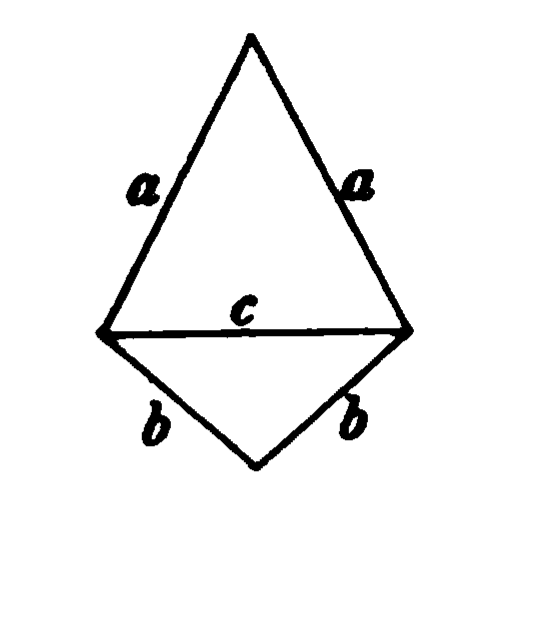
\includegraphics[width=0.18\textwidth]{pdf085-quadrangle.png}
\end{center}

芭蕉葉形の田の面積の半分は、方程式
\[
-(a+b)^3\times10+\left\{\left(\frac a2\right)^2-\left(\frac b2\right)^2\right\}x+x^2=0
\]
によって与えられる。

この田は二つの等しい円弧によって囲まれ、その共通弦は $a$、共通矢高は $b$ である。したがってこの方程式は、弦が $a$、高さが $b$ である円弓形の面積を与える方程式である。

この書には台形の田を等分する問題が含まれる。これは、後代の中国および日本の数学者の大きな注意を引いた同種のさまざまな問題の、最初の例である。問題は次のとおりである。

「舵に似た形の田がある。南辺は小さく 34 歩（$a$）、北辺は大きく 52 歩（$b$）、法長は 150 歩（$h$）である。この田は三兄弟が所有し、彼らに等分しなければならない。分割に際して、一辺に沿って道を設けなければならない。分配された各部分のそれぞれの長さ等を求めよ。」

南辺に来る A の持分の長さについて、方程式
\[
-\frac K2\times h+ahx+\frac{b-a}{2}x^2=0
\]
が与えられる。ここで $K$ は $(a+b)h$ を人数で割った商である。

第八巻で Ch'in は次の問題を与える。

「円形の城があり、その円周と直径は未知である。四つの門を備え、北門の外三里（$a$）に
\scanfooter

\scanpage{0086}{第11章、印刷頁72}
大樹がある。それは南門の東九里（$b$）の一点から見える。城の円周と直径の長さはいくらか。ここでは $\pi$ の旧値を用いよ。」

\begin{center}
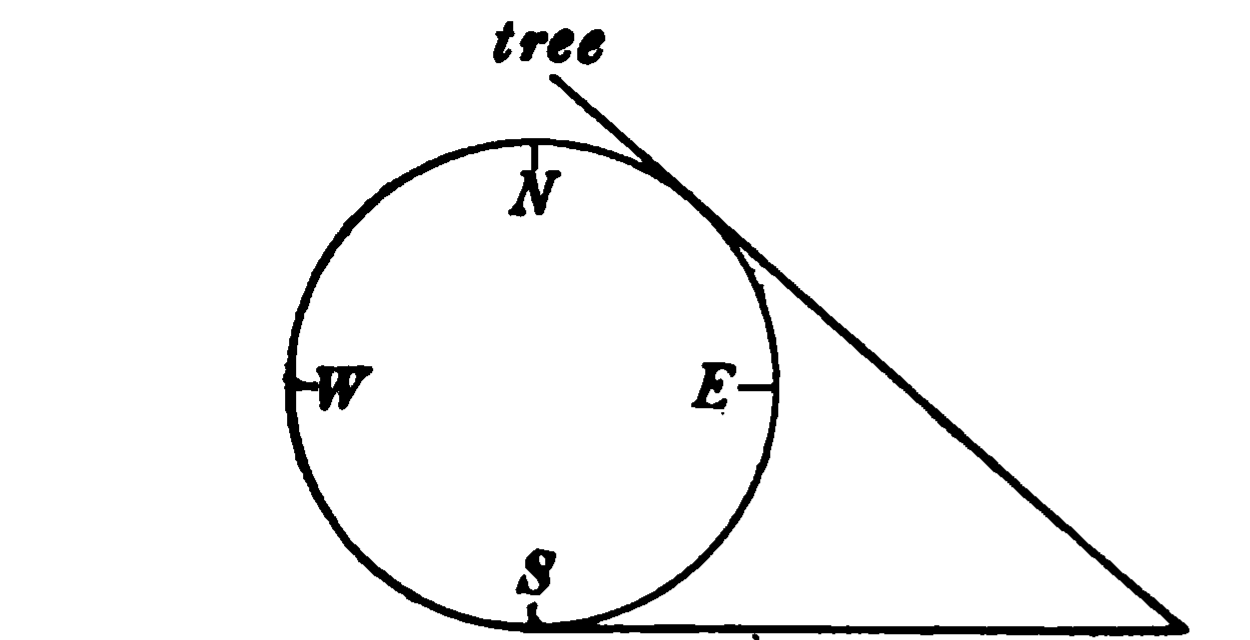
\includegraphics[width=0.45\textwidth]{pdf086-castle-tree.png}

{\small 図中の語句：\emph{tree}＝樹木。}
\end{center}

Ch'in はこれを方程式
\[
1x^{10}+7ax^8+8a^2x^6-4(b^2-a^2)x^2-2b^2\times8a^2x^2-2b^2\times8a^2\times b=0
\]
に従って解き、これは十次のものとして扱われる。

これは直径の長さとして根 $x=9$ を与える。高次方程式の処理が中国数学者のもとで現れるのは、Ch'in の著作が最初であった。

第十四巻の一問題は次のとおりである。

「杉材が三角形に積み重ねられている。積み中の本数は不明であるが、材を中間の部分まで取り去ると、残る層は 9 本から成ることだけが知られている。もとの本数と残りを求めよ。」

これは等差数列の問題であり、Ch'in の与える規則は、そのような数列の和が
\[
=\frac{2(\text{中間層})\times\{2(\text{中間層})-1\}}{2}
\]
に等しいものとして表されることを示す。

第十五巻および第十六巻には、等差数列に関するさらに若干の問題がある。彼は、最初の $r$ 個の自然数の和、および $k$ から $r$ までの和として、公式
\[
\frac{r(r+1)}2\qquad\text{および}\qquad
\frac{r(r+1)}2-\frac{(k-1)k}{2}
\]
を与える。

Ch'in はまた公式
\[
a+(a+b)+\cdots+\bigl(a+\overline{r-1}\,b\bigr)
=\frac b2r^2+\left(a-\frac b2\right)r
\]
を用いる。

第十二巻には、500000 の金額を毎月 100000 ずつ返済するとき、完済に要する月数に関する問題があり、利息は月率 $0\mathbin{\cdot}65\%$ で計算される。この問題を解くにあたり Ch'in は、各支払後の残額を計算するだけであり、一般的処理の方法を用いない。もっとも、他の
\scanfooter

\scanpage{0087}{第11章、印刷頁73}
箇所では高次方程式を用いる。彼はおそらく、幾何数列の数の和を与える一般公式を知らなかった。

第十七巻では、連立一次方程式の古代の処理が、付図のような形で書かれている。もちろん文字は、算木の配列形を表す数字で記録された数を表すためのものである。Ch'in が連立系について筆算的操作に頼ったと考えてはならない。彼は、算木盤上に配列され実行されるべきものを書き下しているだけだからである。

\begin{center}
\renewcommand{\arraystretch}{1.25}
\begin{tabular}{|l|c|c|}\hline
重量 & $a$ & $a'$ \\ \hline
塩 & $b$ & $b'$ \\ \hline
銀 & $c$ & $c'$ \\ \hline
\end{tabular}
\end{center}

Ch'in がその著作で用いる数字は、しかも実際にその全篇で非常に自由に用いる数字は、Sun-Tsŭ についての考察に関連してわれわれが示した算木配列とほとんど異ならない。さらに彼は、零に $\bigcirc$ の記号を用いた。\rodglyph{1.45em}{pdf087-rod-numeral-4.png}、\rodglyph{1.45em}{pdf087-rod-numeral-5.png}、\rodglyph{1.45em}{pdf087-rod-numeral-9a.png}、\rodglyph{1.45em}{pdf087-rod-numeral-9b.png} のような記号も、4、5、9 を示すために用いられ、最後の二記号はいずれも 9 を表す。Ch'in の記法では、位取りの原理が厳格に守られる。しかしこれは不思議ではない。それは、算木盤上に配列されるべきものを書き下す一方法にすぎず、そこでは同じ原理が太古から守られていたからである。零号は確かに Indian の源から、おそらく現在失われている \emph{Chiu-chih-Li} の中国語訳を通じて借りられた。その使用は、われわれの知る限り Ch'in の著作に初めて現れるが、それでも Ch'in が中国でこの記号を最初に用いた人物であった可能性はほとんどない。

われわれは、Ch'in Chiu-shao が若干の問題を解く際に高次方程式に頼ったことを述べた。彼はまた、そのような方程式を解く実際の段階を詳しく説明する。ここでわれわれは、Ch'in が行った数値方程式の根を抽出する実際の過程を記述しなければならない。

すでに見たように、中国人は古代から算木、すなわち sangis を用いて算盤算術を実践した。彼らは算木盤上で平方根と立方根を抽出し、実際、両者とも同じ原理によった。少なくとも Chang T'sang と Ching Ch'ou-ch'ang の時代には、すでに二次方程式さえ解いていた。そのような解法は、おそらく平方根抽出と同じ道筋で行われた。七世紀初めには Wang Hs'iao-t'ung が三次方程式の適用によって多くの問題を解いた。Wang はたしかに、その方程式を解く
\scanfooter

\scanpage{0088}{第11章、印刷頁74}
実際的方法を示してはいないが、彼が明言するところによれば、それらは立方根抽出と同じ仕方で処理されなければならなかった。

このように、数値方程式を近似的に解く方法は、早い時代から中国人に無縁ではなかった。しかし、Ch'in Chiu-shao の著作に至るまで、第三次'より高い次数の方程式の例は現れなかった。彼の解法でさえ新しい原理に基づくものではなく、二次および三次の根抽出法と、旧時代に行われた二次方程式および三次方程式の推測された過程との自然な拡張であった。それにもかかわらず、彼の説明または拡張は、中国数学の進歩に不可欠であった。この数値方程式解法は、若干の西洋学者が推測したような筆算ではなく、算木盤上で行われた。私の見解が正しいならば、算木の実践だけが、中国人を高次数値方程式の解法という、かくも評価すべき過程の確立へ導いたのである。

Ch'in はまず、その著作第四巻で四乗根の抽出を例示する。次いで次章において四次方程式
\[
-x^4+763\,200x^2-40\,642\,560\,000=0
\]
の解法へ進む。

Ch'in はこの方程式を $x^2$ の二次方程式として扱わず、四次方程式として解く。

Ch'in が、そして彼とともに他のすべての中国数学者が、定数項を常に負とすることは注目に値する。

Ch'in の著作の原本では、正数と負数を、正負の算木の色に従って赤色と黒色で書き分けた、と述べられている。

まず、われわれの前の方程式は次の形に配列される。

\begin{center}
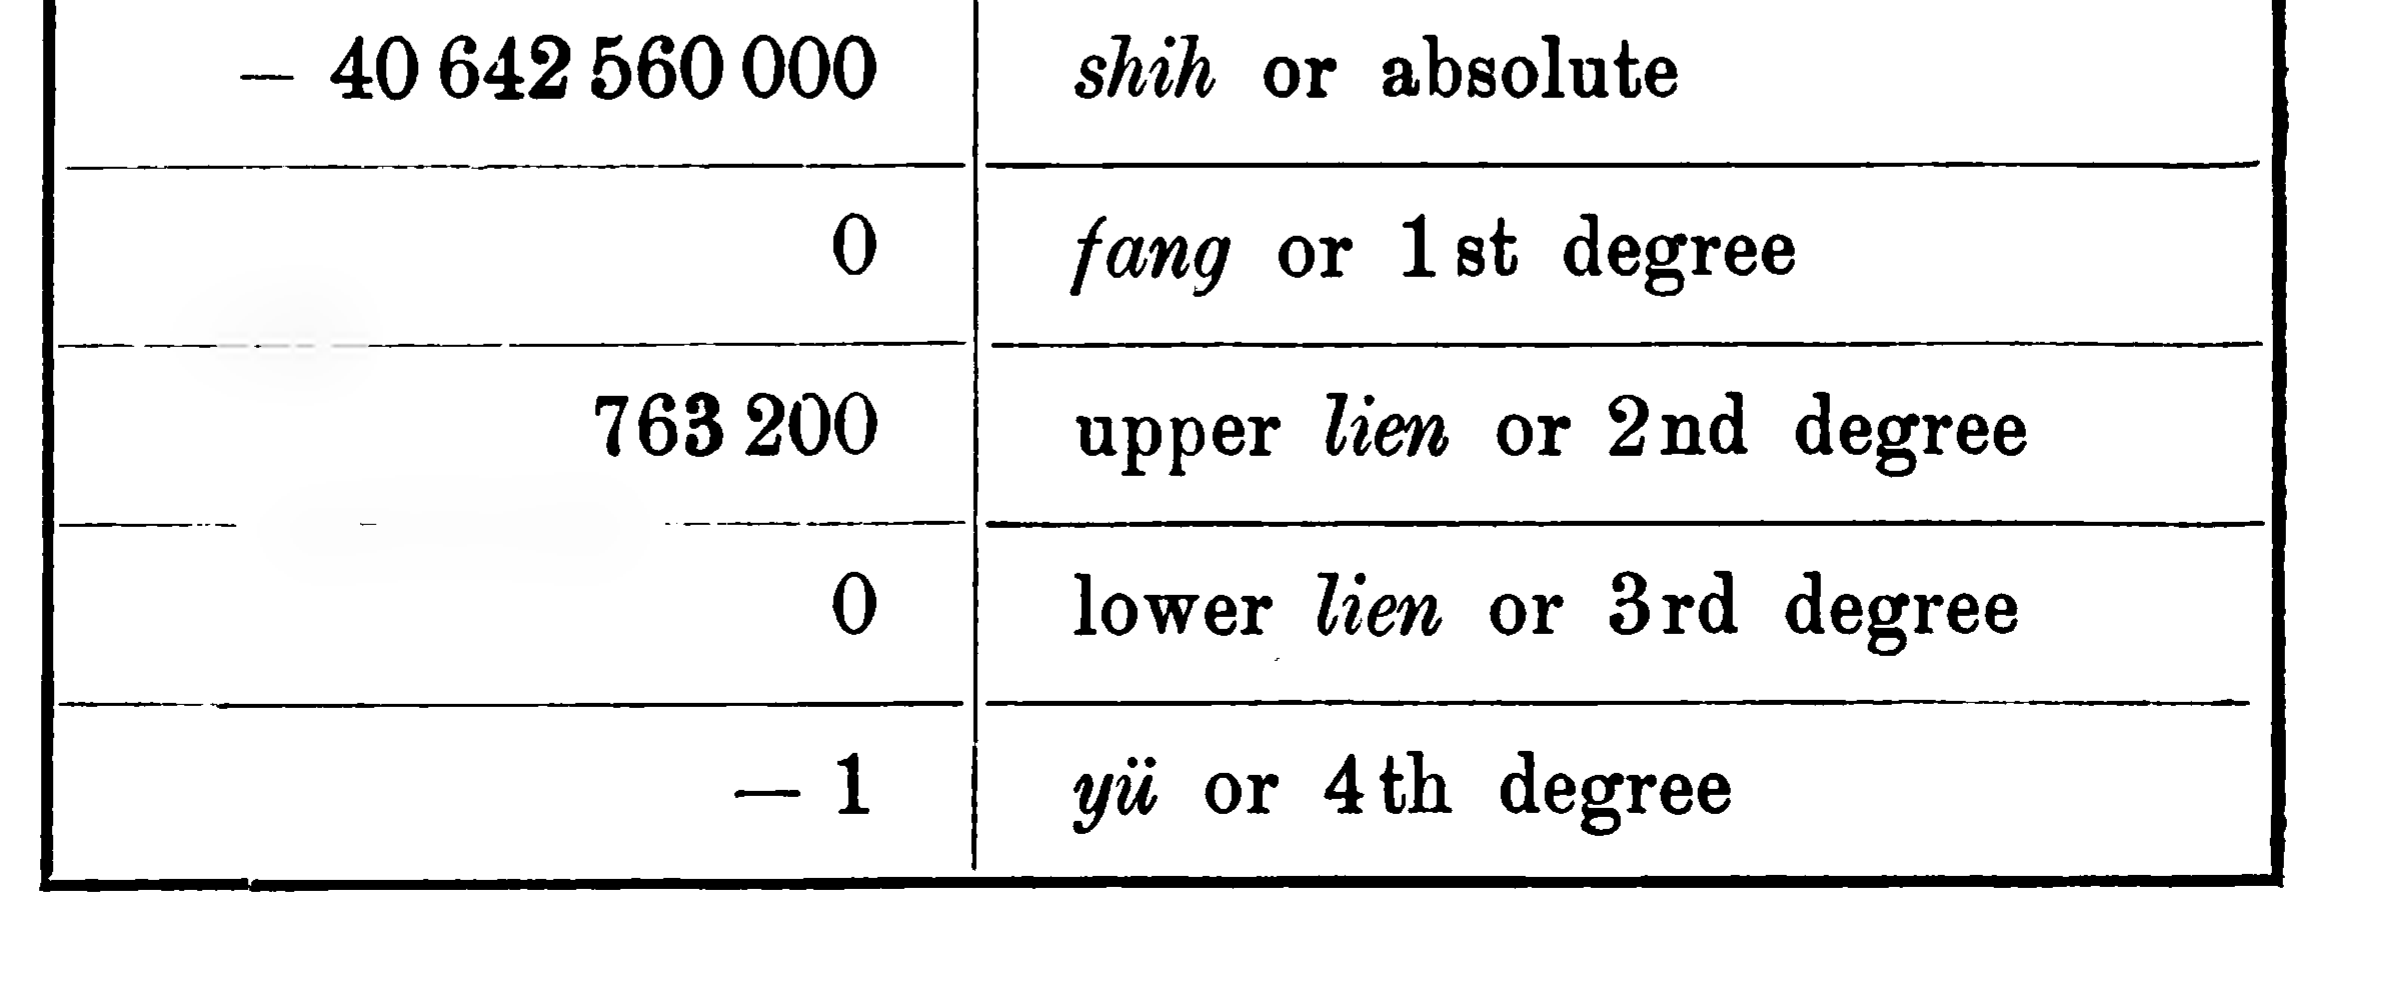
\includegraphics[width=0.94\textwidth]{pdf088-initial-root-arrangement.png}

{\small 図中の語句：\emph{shih}＝定数級、\emph{fang}＝一次級、\emph{upper lien}＝上廉すなわち二次級、\emph{lower lien}＝下廉すなわち三次級、\emph{yü}＝四次級。}
\end{center}
\scanfooter

\scanpage{0089}{第11章、印刷頁75}
根の開出を行うため、定数級を除く各級を、平方根および立方根抽出の場合と同じく、左へ移さなければならない。この移動は、一次級を一列、二次級を二列、三次級を三列、四次級を四列進めるように行うべきである。われわれの前の例では、同じ過程を二度繰り返さなければならず、したがって根が三桁であることが知られる。連続する各段階は Ch'in の著作では別々の図に示されているが、著者のたどる全過程を再録するのはあまりに冗長なので、ここではその過程を略式で説明する。

根の最初の数字は 8 と分かり、これを四次級に掛け、その結果を代数的に 3nd 次級へ加える。この結果を根で掛け、代数的に二次級へ加える。さらにその結果を根で掛け、代数的に一次級へ加える。この結果を根で掛け、定数級から引く（または代数的に定数級へ加える）。結果は次のとおりである。

\begin{center}
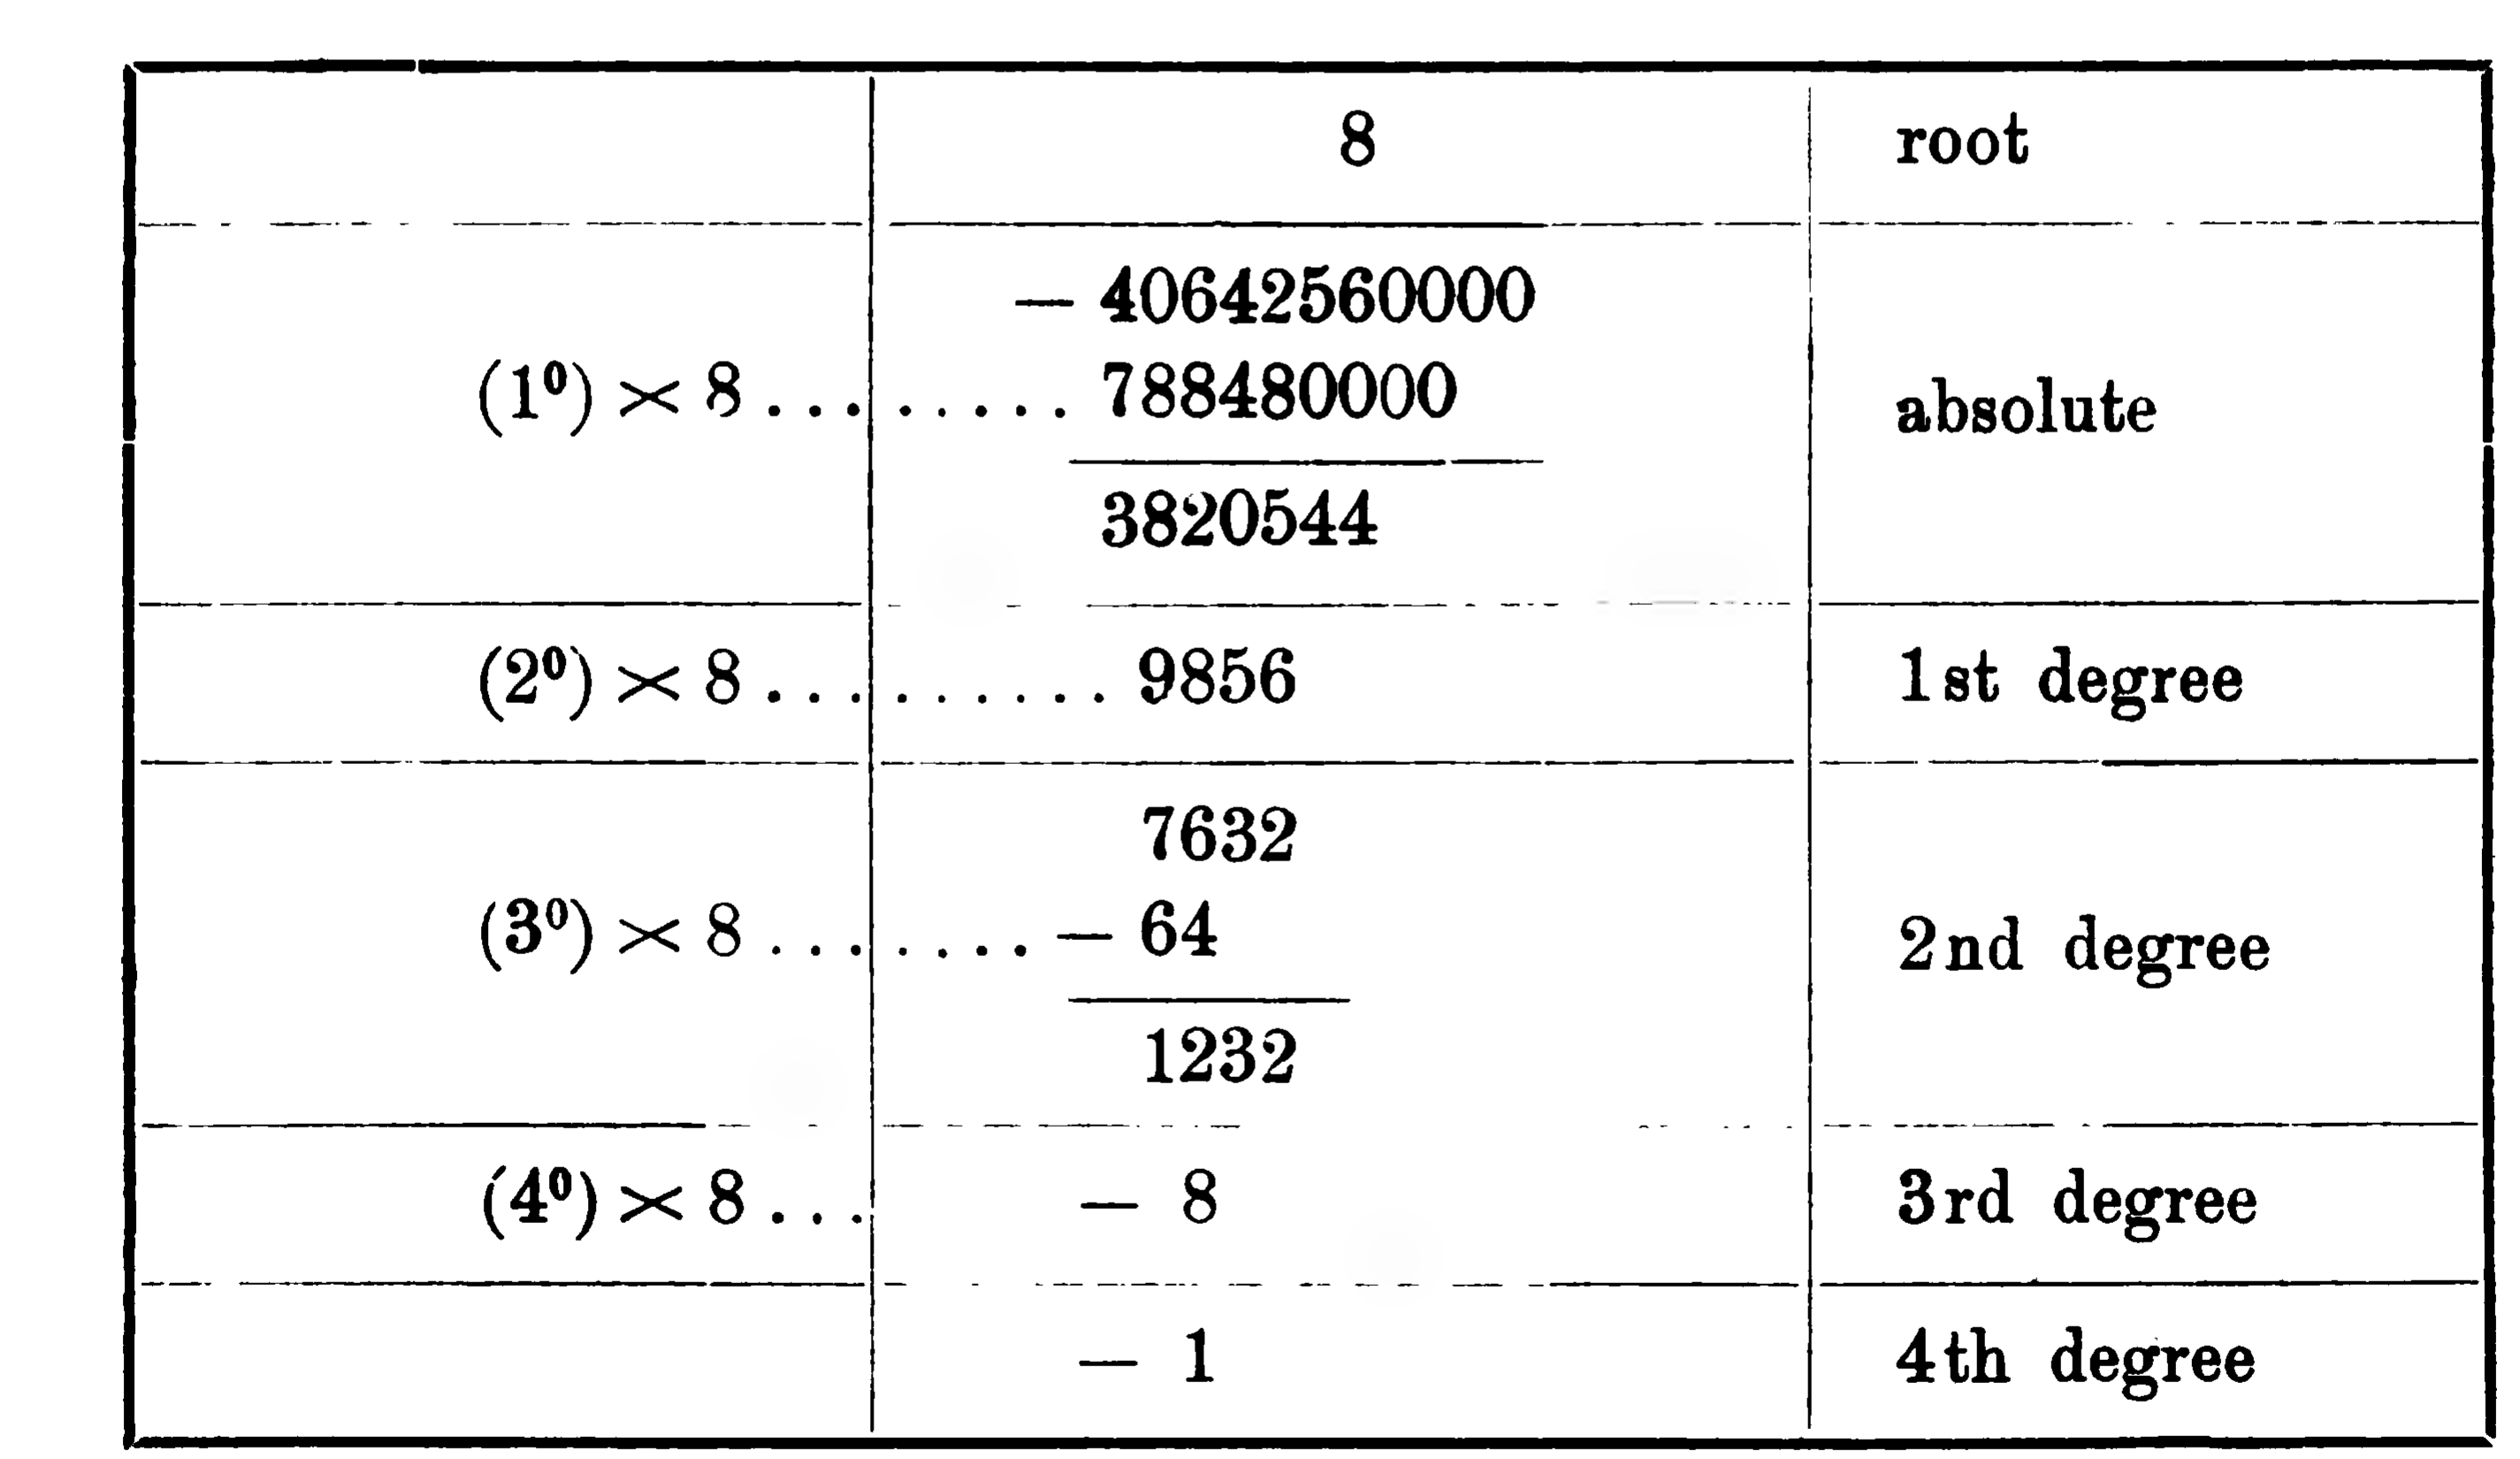
\includegraphics[width=0.94\textwidth]{pdf089-first-root-figure.png}

{\small 図中の語句：\emph{root}＝根、\emph{absolute}＝定数級、\emph{1st degree}＝一次級、\emph{2nd degree}＝二次級、\emph{3rd degree}＝三次級、\emph{4th degree}＝四次級。}
\end{center}

次に、新しく得られた式において根を四次級に掛け、その積を代数的に三次級へ加える。この結果を根で掛け、その積を代数的に二次級へ加える。この結果に根を掛け、その積を代数的に一次級へ加える。
\scanfooter

\scanpage{0090}{第11章、印刷頁76}
再び四次級を根で掛け、その積を代数的に三次級へ加える。この結果に根を掛け、その積を代数的に二次級へ加える。

再び四次級を根で掛け、その積を代数的に三次級へ加える。

これらの操作の結果は次のとおりである。

\begin{center}
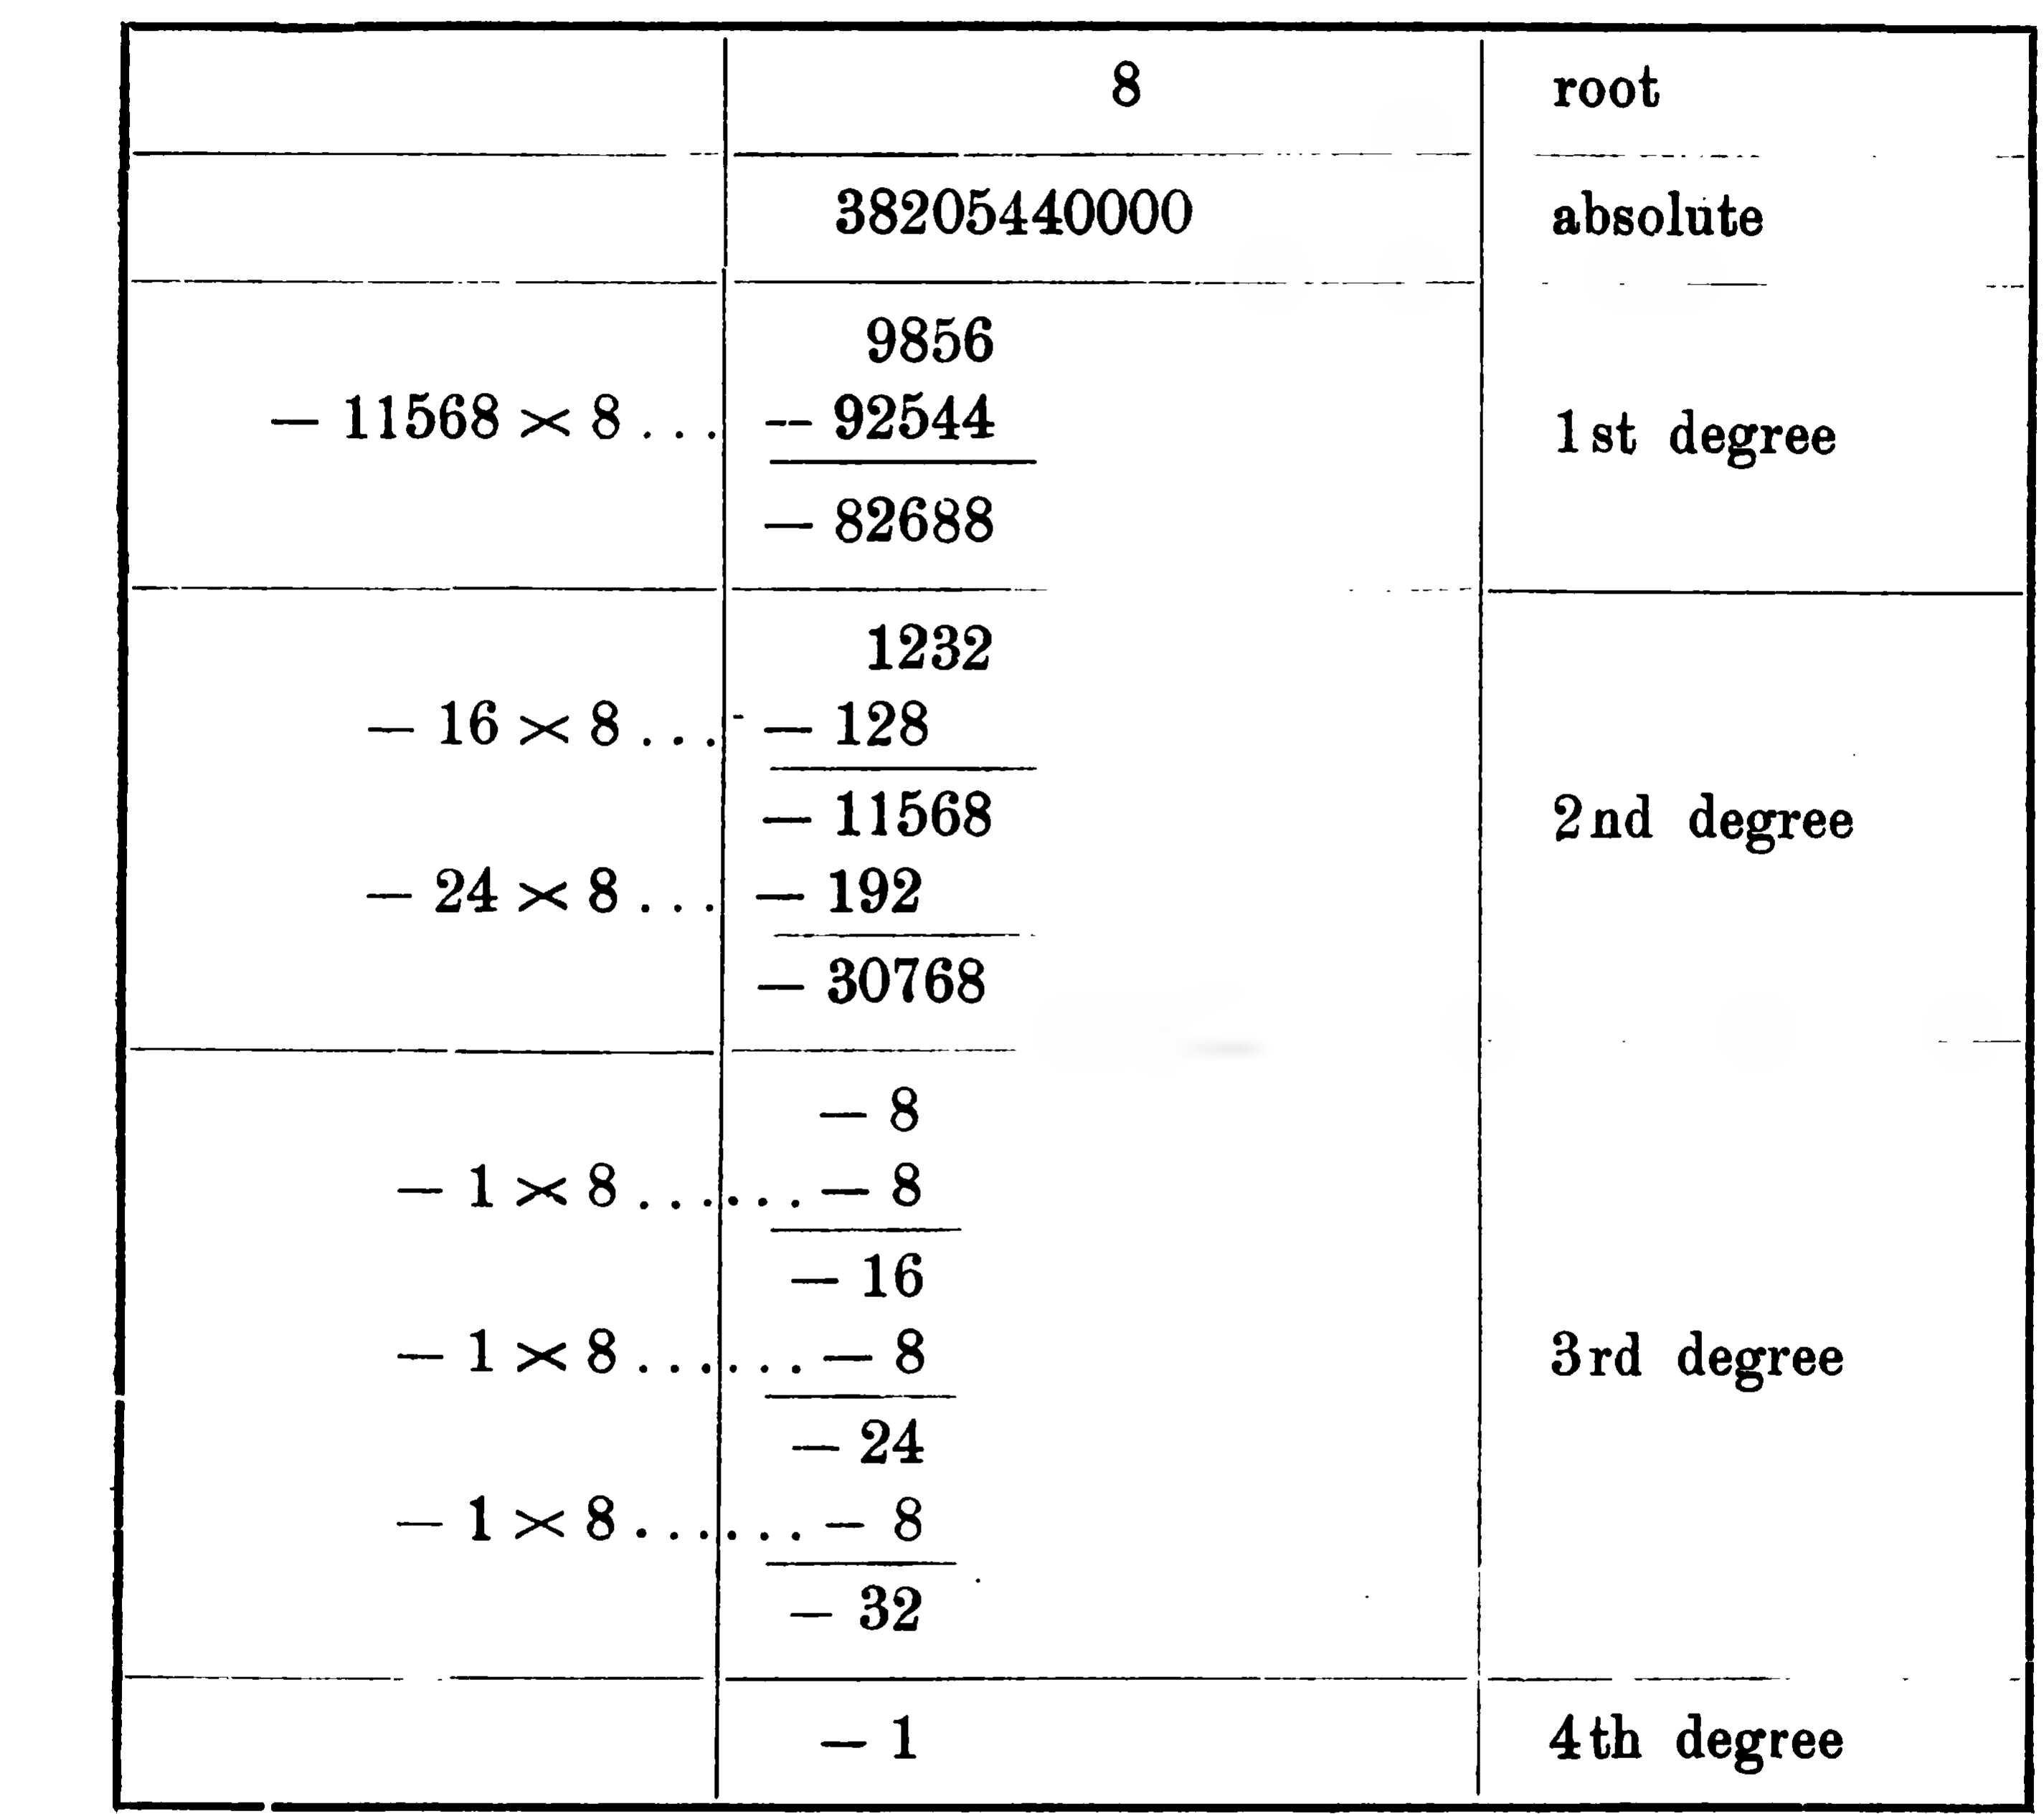
\includegraphics[width=0.92\textwidth]{pdf090-root-operations.png}

{\small 図中の語句：\emph{root}＝根、\emph{absolute}＝定数級、\emph{1st degree}＝一次級、\emph{2nd degree}＝二次級、\emph{3rd degree}＝三次級、\emph{4th degree}＝四次級。}
\end{center}

次に、一次、二次、三次、四次の各級を、それぞれ 1、2、3、4 列だけ右へ戻す。こうして配列は次頁に示す形を取る。

いま根の第二の数字として 4 を取り、まったく同じ仕方で進める。同様の操作を続けて繰り返せば、根のさらに後の数字の評価に至る。しかしこの例では、根の第二の数字について操作を行った後に定数級が消滅するので、開出はここで終わり、根 $=840$ を与える。
\scanfooter

\scanpage{0091}{第11章、印刷頁77}
以上に記述した、中国人が方程式の根を抽出する実践を知るとき、数値方程式の近似解法に対する著名な Horner の方法を想起せずにはいられない。両者が原理の諸点においていかに同一であるかを見よ。

\begin{center}
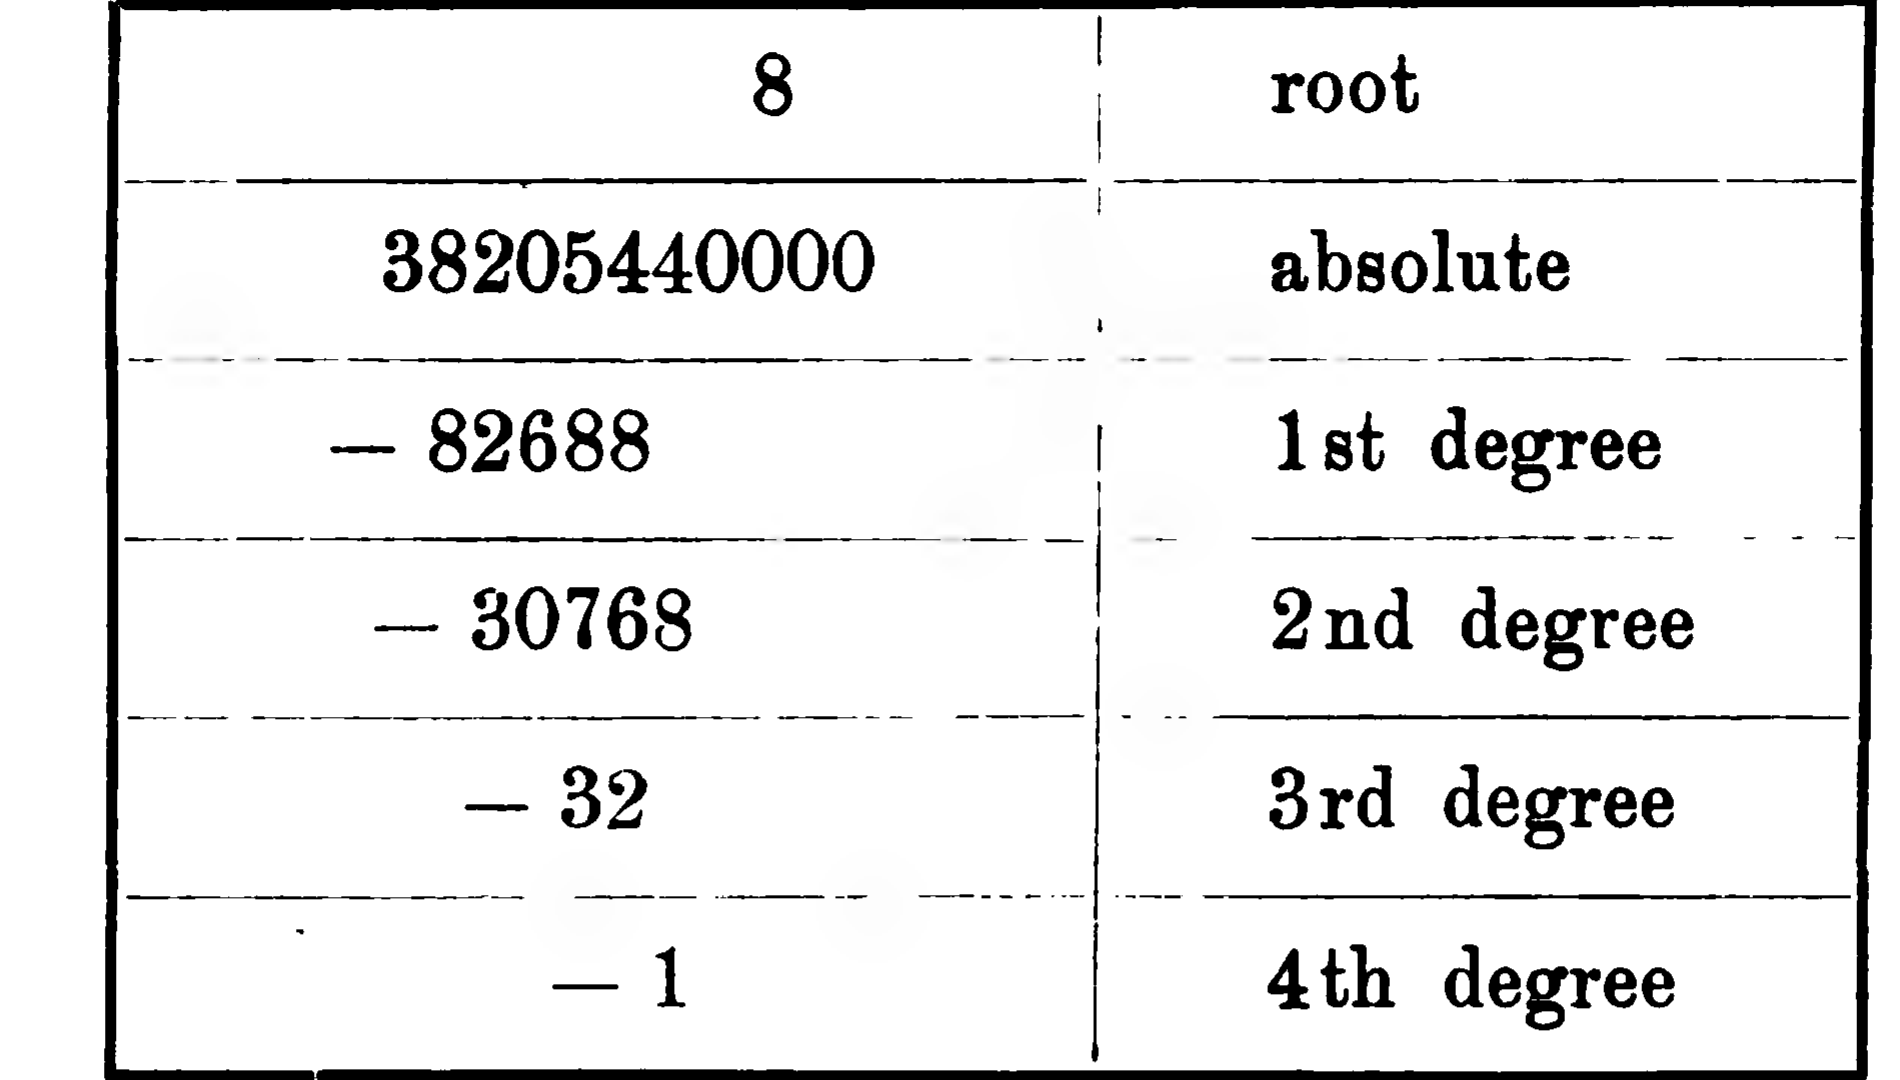
\includegraphics[width=0.68\textwidth]{pdf091-shifted-root-arrangement.png}

{\small 図中の語句：\emph{root}＝根、\emph{absolute}＝定数級、\emph{1st degree}＝一次級、\emph{2nd degree}＝二次級、\emph{3rd degree}＝三次級、\emph{4th degree}＝四次級。}
\end{center}

二つの方法に何か相違があるとすれば、それは配列法の相違に求めるべきであり、それは当然、操作体系の相違による。中国人は算木盤上で方程式を解いたが、Horner は筆算を用いた。いずれにせよ、Horner の論文が一八一九年に刊行されたのであるから、Horner の著名な過程が Europe より少なくともほぼ六百年も早く中国で用いられていたという事実を、誰が否定しえようか。もちろんわれわれは、Horner の発明をいかなる仕方でも中国起源に帰そうとはしない。しかし時間の経過を考えれば、Europe 人が直接または間接に中国の方法を知っていた可能性が、まったくありえないとはいえない。さらに Europe 人は、Occidental の諸科学を Middle Empire の地へ移植するため、二世紀以上にわたって中国人と活発に協力していた。その中には数学に通じた者も少なくなかった，なぜ彼らは、眼前に公然と置かれていた中国代数の方法に接触しえなかったのか。十七世紀に Europe の代数、すなわち数値方程式を解く過程が中国へ導入された際の中国人の感情については、現在の Ching 王朝下における中国人の数学的到達を論ずるとき、再び若干述べることにする。

いま述べた過程は、後代の中国数学者および日本数学者が行ったように、根の小数部分の評価にも同様に適用される。しかし Ch'in はその種のことを何も試みなかった。
\scanfooter

\scanpage{0092}{第11章結尾、印刷頁78}
$\sqrt{1000}$ の開方において Ch'in は根を $31\frac{13}{21}$ と与え、その分数部分は旧時代に行われたのと同じ仕方で導かれる

彼は同じ処理を方程式の場合に適用する。方程式
\[
(a+b)^3\times10=\left\{\left(\frac a2\right)^2-\left(\frac b2\right)^2\right\}x+x^2
\]
において、$a=576$、$b=34$ とすると、Ch'in はまず根の整数部分を 21742 と計算し、そのとき定数級には量 10426 が残る。次に Ch'in は、次の操作で必要となる一次級を計算し、この量は 126140 と求められる。ここで根の半分を求めるため、Ch'in はこれらの量の半分を取り、
\[
(\text{根})=10871\frac{5213}{63070}
\]
と置く。ここで分母は誤って半分にされたのかもしれない。

Thomas Harriot（一五六〇---一六二一）が、方程式のすべての有意項を等号の一方に置いたことは、歴史上著名な事実である。Ch'in は定数項を常に負となるように配列し、これは Harriot の業績に非常によく似ている。Ch'in と同時代の Li Yeh、および後代の他のすべての数学者は、Ch'in の著作に示された同じ配列法に従った。したがってこの点で、中国人は Harriot より三世紀以上先んじていたといえる。

Ch'in Chiu-shao は一方では、数値方程式の開出または根抽出の過程を説明することにきわめて綿密であったにもかかわらず、他方では、問題に与えられたデータから代数的考察によってそのような方程式を構成する方法の記述を完全に怠った。しかしこれは、彼が代数的処理にまったく無縁であったことを意味しない。そうであるならば、彼がその著作で用いたこれらの複雑な方程式へ、どうして導かれえたであろうか。しかし代数的操作の説明は、Mongol 侵略者の対立王朝に遠く離れて住んだ、同時代人 Li Yeh の手に残された。いまわれわれは、この数学者の生涯について若干を概観することへ移る。
\scanfooter


\scanpage{0093}{第12章冒頭、印刷頁79}
\setcounter{footnote}{0}
\begin{center}
第12章。\\
LI YEH。
\end{center}
\phantomsection\addcontentsline{toc}{subsection}{第12章　LI YEH}

一二四八年、Ch'in Chiu-shao が \emph{Su-shu Chiu-chang} を著した翌年に、Li Yeh の著した \emph{T'sê-yüan Hai-ching}、すなわち「円測海鏡」が現れ、これに一二五九年の \emph{I-ku Yen-tuan} が続いた。われわれが Ch'in の著作を高く評価してきたのと同じく、この二著も歴史上きわめて貴重である。伝存する古文献の範囲では、中国人の手によって代数的考察が初めて説明されているのが、まさにこれらの著作だからである。Ch'in が、得られた方程式を解く過程の説明だけに注意を集中し、その構成についてはほんのわずかな示唆すら与えなかったのに対して、Li は、十分ではないにせよ、問題に与えられた資料から解に必要な方程式を構成するまでの進み方を述べようとしただけで、その実際の解法は示さなかった。このことから、Ch'in と Li は同じ時点に現れ、中国代数に必要な基礎を十分に備えるため、相協力したかのように見えないだろうか。しかし二人は遠く隔たって暮らし、しかも相争う別々の王朝に属していた。

\emph{Sung-Shih}、すなわち「宋史」は Ch'in の伝記を載せないが、\emph{Yuen-Shih}、すなわち「元史」は、その列伝に Li Yeh の生涯を載せる。この記録によれば、Li Yeh\footnote{Li Yeh は、ときに（Moritz Cantor などによって）Li-yeh Jin-king と表されるが、姓は Li、個人名は Yeh であった。Jin-king は彼の字、すなわちすべての中国人が持つ別名であった。} は、中国北部に位置し、Sung と絶えず争っていた Chin 王朝の支配下にある Luan-ch'êng に生まれた。彼は Chin 政府の官吏登用試験に合格し、しばらくして Chün Chou の知事となったが、一二三二年にその州城が敵の手に落ちた。Li は姿を変えて逃れ、貧窮のうちに暮らした。その後、集め得た書物の研究に身を捧げた。Chin 王朝が滅亡した後\footnote{Chin 王朝は一二三四年に Mongol の侵入者によって滅ぼされた。}、Mongol の王子 Kublai Khan は、彼の賢明さを知ったため、彼を召し出した 当代の賢者について有力な王子から問われると、Li Yeh は直ちに答えた。「世に賢者が絶えることは決してない。もしあなたが彼らを求めるならば、
\scanfooter

\scanpage{0094}{第12章、印刷頁80}
彼らはあなたの前に現れる。しかし、もし求めなければ、賢者は一人も現れない。これはただ明白な一つの理由によるだけである」。

さらに国を治める分別について問われると、Li Yeh は王子に対し、徳ある者を登用し、不徳の者を退けるべきこと、規則を厳守し、秩序を保たねばならないことを真摯に説いた。彼は当時の弊害について明言することさえ恐れなかった。

Li Yeh の返答はすべて Kublai Khan に認められ、彼は高く尊重された。しかし、その時点では Mongol に仕えなかった。

晩年、Li Yeh は Mongol の領土に住み、弟子を教えた。弟子は時とともにますます多くなった。Kublai Khan が一二六四年に即位すると、Li は再び召されたが、年齢と病弱を理由に、またも仕官を辞退した。しかし翌年、重ねて懇請され、Han-lin Academy の一席に就くことを余儀なくされた。そこにいたのはわずか数か月で、職を辞して去った。その後、八十七歳で没した。後世の著者のうち、十八世紀末から次世紀初頭に活躍した Chiao. Hsün などは、Li Yeh の没年を一二六五年とする。

「元史」によれば、Li Yeh は、すでに述べた二著のほかにも、Ching-chai が Li Yeh の号であるところの、四十巻から成る \emph{Ching-chai Wen-chi}、すなわち「Ching-chai 文集」、十二巻から成る \emph{Pi-shu Su-hsiao}、四十巻から成る \emph{Fan-shuo}、四十巻から成る \emph{Ku-chin Nan}、すなわち「古今批評」などの著作を残した。

「円測海鏡」は、その標題が示すとおり、円に関係する測定を扱うことを意図したものであったが、その処理は円積問題の領域には属さない。著者がこの書の序文に記すところでは、彼は若年から数学研究に親しんでいたが、円に関する計算について何一つ確定していないことを常に遺憾としていた。たとえば、古い $\pi$ の値と Liu Hui および Tsu Ch'ung-chih の値とはすべて異なっており、また円弧、矢、および円弧部分の面積を彼の満足する仕方で測る方法はなかった。しかし五十四歳を過ぎてから、彼は \emph{T'ung-yuen Chiu-yung} の学説に出会い、これを非常に興味深いものと認めた。これはおそらく
\scanfooter

\scanpage{0095}{第12章、印刷頁81}
天元の代数的考察の方法であった。しかし実を言えば、後代の中国人著者たちは皆、この語の意味を明らかにできずにいる。いずれにせよ、Li Yeh はこうして示された学説または術を注意深く研鑽し、ついには長く彼を悩ませていた諸問題について満足を得た。

このような予備的説明を述べたのち、Li Yeh は「円測海鏡」の十二巻または十二章において、その規則を立て始める。著作の冒頭で、彼はまず次図のような図を掲げる。

\sourceasset{0.47\textwidth}{pdf095-li-yeh-diagram.png}

第一巻または第一章では、Li Yeh はこの図の各部分の関係を説明し、第二巻以下は、これらの量に関係するさまざまな計算法の考察に充てられる。処理は代数的方法による。

同じ著者の後の著作 \emph{I-ku Yen-tuan} も代数的処理に充てられた。しかし、代数式の表し方はこの二著で異なる。

われわれはすでに、Ch'in Chiu-shao が天元を意味する \emph{t'ien-yuen} という語を用いたことに言及した。同じ語は Li Yeh にも用いられた。すでに述べたとおり、Ch'in は不定問題の処理において天元に言及したが、歴史上きわめて著名となった数値方程式の操作との関係では、この語を用いなかった。Li Yeh が天元という語を用いたのは、この後者の関係においてであった。

Li Yeh の天元代数の過程では、一が未知数の代表として用いられる。これは確かに算木を用いてなされた。しかし著作に書き記す際、Li は式中の他の項と区別するため、その一の傍らに「元」という表意文字を書いた。各項は縦一列に配列される。定数項は一次項の下に置かれ、「太」という表意文字で標示される。それはおそらく、\emph{tai-chi}、すなわち極限または大極の位置を占めることを意味する。天元の平方は
\scanfooter

\scanpage{0096}{第12章、印刷頁82}
天元の直上に置かれ、その上に立方が来て、以下順次上方へ続く。したがって方程式
\[
x^3+15x^2+66x-360=0
\]
は、付図のように書かれる。

\sourceasset{0.54\textwidth}{pdf096-equation-arrangement.png}

平方項およびそれ以上の項は明示的に標示されないが、大極すなわち定数項に対する相対的位置によって示される。実際には「元」と「太」の二字はともに必要ではなく、その一方を省く方が都合よい。

「円測海鏡」に見られる Li Yeh の方程式配列法は、古来の開方過程の発展に従った Ch'in のものとはまったく異なる。だが、どのような理由が著者にこの配列を採らせたのかは、われわれにはまったく分からない。しかし \emph{I-ku Yen-tuan} では、Li Yeh は配列を Ch'in と同じ仕方に変え、定数項を最上部に置き、他の項を順次その下に置いた。そして、この方式が以後一般に行われることとなった。

Ch'in Chiu-shao は正数を赤色、負数を黒色で書いて区別した。これが Ch'in 自身の発明であったか否かにかかわらず、これはきわめて自然であった。中国人はそれ以前から長く、正負の数を区別するために赤と黒の算木を用いることに慣れており、方程式は最終的にこれらの算木で配列されるはずだったからである。しかし、書写、とりわけ印刷に二色を用いるのは便利でない。そこで、書面で異符号の数を表す際、特別に設計された記号によって区別する慣行がほどなく生じた。このような記号は Li Yeh の二著にともに見られる。彼がこの記号を用いた最初の中国人であったかどうかは確かでないが、その著作は、おそらく現代まで伝わる使用例を含む最古の文献である。この記号は、右端の数字を斜めに横切る一画から成る。したがって

\sourceasset{0.73\textwidth}{pdf096-negative-numeral-forms.png}

は、それぞれ $-10724$、$-9$、および $-10200$ を表す。
\scanfooter

\scanpage{0097}{第12章、印刷頁83}
零を表す記号 $\bigcirc$ も、Ch'in と Li の双方によって用いられた。

この零記号は、Li Yeh による負数の標示法とともに、それ以来絶えず用いられてきた。封建時代の日本数学者も、これらの記号を用いた。

Ch'in Chiu-shao と Li Yeh は同時代の学者であり、同時期に方程式の処理を教えた。このため、一部の学者は後者が前者の著作の影響を受けたと考えた。しかし後代の中国人学者の多数は、二人が相争う王朝の遠隔地に住んでいたため、両数学者の成果を互いに独立して作り上げられたものと考える点で一致しているようである。われわれもこの見解を受け入れる。しかし、両者が同じ \emph{t'ien-yuen}、すなわち天元という語と、零の同じ記号 $\bigcirc$ を用いたことは説明を要する。二人の独立した研究者による同時発明から、そのような一致が生じることはあり得ないからである。したがって、天元の実践と零記号の使用は、この二人の時代より前から存在していたと結論するのが適切であろう。零記号は、おそらく T'ang 王朝の時代に India から導入された。Ch'in と Li が自著の序文に記したことは、きわめて乏しいながらも、われわれの見解を正当化するように思われる。

次章では、われわれの二著者より少し後の日付を持つ著作を残し、同じ事柄を扱った同時代の学者の仕事について若干述べる。

半世紀後、Chu Shih-chieh という数学者が現れ、一三〇三年に \emph{Szu-yuen Yü-chien} を著した。この書の序文によれば、Chin 王朝の文官であった Yuen Hao-wen という人物がいたことが分かる。その帝国の滅亡後、彼はさまざまな主題について著述して日々を送り、数学、とりわけ天元法に通じていた。彼は Li Yeh の友人であり、親しい交友関係にあった。Yuen はかつて、Liu Ju-hsieh の著した \emph{Ju-chi Shih-hsiao} という数学書に詳細な注釈を書いた。これはほぼ確実に天元代数の著作であったが、Liu の原著も Yuen の注釈も現存しない。Liu の生存年代も知られていない。

天元代数は、十三世紀に生じた新発明では決してなく、前代から伝わってきたものと思われる。
\scanfooter

\scanpage{0098}{第12章結尾および第13章冒頭、印刷頁84}
しかし同時に、当時、天元が数学者の全体に広く実践されていたわけでもなかった。Li Yeh が以前用いた配列法を後の著作で変えたという一事だけでも、そのような慣行が彼の同時代人の間で非常に一般的ではなかったことを十分に示す。Li Yeh が臨終の床で息子にその著作を託したとき、「円測海鏡」をいかに重視したかを見よ。一二八七年に「円測海鏡」を再刊した Wang Tê-yüan によれば、Li Yeh は死に際して息子に、\emph{T'sê-yüan Hai-ching}、すなわち「円測海鏡」一書を除き、自分の著作をすべて焼くよう命じ、後世が必ずその内容を尊ぶようになると確信している、と述べた。

いずれにせよ、中国代数は平方根および立方根の抽出を考える古い実践から生じた。Li Yeh とその後継者によって扱われた中国代数は、算木盤上で操作された。これは中国数学に特有のものであった。中国人が代数操作の方法を外国の何らかの源から借用したと疑う理由は、まったくない。

次章では、天元方程式に再び出会う別の数学者について述べる。

\begin{center}
第13章。\\
YANG HUI。
\end{center}
\phantomsection\addcontentsline{toc}{subsection}{第13章　YANG HUI}

Ch'in Chiu-shao と Li Yeh の著作が現れた直後、Yang Hui という第三の数学者が現れた。彼は Ch'ien-t'ang の出身で、Sung 王朝に属した。その生涯について、われわれはほとんど何も知らないが、今日まで保存された彼の著作を数点所有している。これらは、旧「九章」の規則と問題の一部を説明する、一二六一年の \emph{Hsiang-chieh Chiu-chang Suan-fa}、すなわち「九章算術詳解」；「九章詳解補遺」；および Yüan Yüan が \emph{Yang Hui Suan-fa}、すなわち「Yang Hui 算法」と呼ぶ他の五著であり、その一つには一二七五年の日付がある。

「九章詳解」で Yang Hui は等差級数の総和を例示する。第一日に一九三中国里（\emph{li}）を進み、毎日速度を十五里ずつ増す駿馬が、十五日間に進む総距離を求めるため、Yang
\scanfooter

\scanpage{0099}{第13章、印刷頁85}
Hui は、日数と、初日の速度と最終日の速度との和の半分との積を取る。最終日の速度は、初日の速度に一日の速度増加量の十四倍を加えて求められる。ここで彼は付図のような図を加える。

\sourceasset{0.68\textwidth}{pdf099-speed-diagram.png}

Yang が、必要な答えは、この図を二つ合わせてできる長方形の面積に対応する量を取り、その結果を半分にすることで得られることを示そうとしているのは明らかである。

\emph{Suan-fa T'ung-pien Pen-mo} で Yang Hui はさらに、彼が三角級数および平方級数と呼ぶ級数の和の公式を与える。それらは
\[
1+(1+2)+(1+2+3)+\cdots+(1+2+3+4+\cdots+n)
=\frac{n(n+1)(n+2)}{6},
\]
\[
1^2+2^2+3^2+\cdots+n^2
=\frac{1}{3}n\left(n+\frac{1}{2}\right)(n+1).
\]
である。

これらの級数について与えられるのは、公式、あるいはむしろその公式に至る規則だけであり、その解析については何の説明も試みられていない。

すでに述べたとおり、\emph{Wu-tsao Suan-ching} は、四辺形の面積を、対辺二組の半和の積として誤って与える。Yang Hui はその誤りを認識し、「詳解補遺」で訂正を試みた。彼は、辺が順に 35、15、45、25 である四辺形を考える。35 と 25 の辺が作る頂点から 45 の辺へ垂線を下ろし、四辺形を二部分に分けて面積を計算する。垂線は $22\cdot44995$ とされ、二部分は直角三角形と台形として扱われる。この関係が成り立つのは 15 と 45 の辺が直角をなす場合だけであるが、著者は他の可能性の存在について何も述べない。

Yang Hui は「補遺」で単比例の問題を考え、その一つは次のとおりである。「A は 100 歩（$a$）走る間に、B は 60 歩（$b$）走る。いま B が A より 100 歩（$c$）先から出発するとすれば、後者は何歩で前者に追いつくか。」
\scanfooter

\scanpage{0100}{第13章、印刷頁86}
この問題は明らかに、比例式
\[
a:a-b=c:x
\]
によって解くことができ、これがまさに Yang Hui の用いる公式である。彼はこれを付図の形に書き、二つの項を交乗し、その結果を残る項で割るだけである。

\sourceasset{0.24\textwidth}{pdf100-proportion-cross.png}

比例問題は「九章」で考察されていたが、比例を表すこの形式は、われわれの限られた知識の範囲では、Yang Hui によって初めて示された。彼は比例を \emph{hu-huan}、文字どおりには「交互交換」と呼ぶ。\emph{Hsü Ku-chai-ch'i Suan-fa} では複比例の問題も扱い、これを \emph{chung hu-huan}、すなわち「二重交互交換」と呼ぶ。

一次方程式では、Yang は四個または五個の未知量を含む問題を考察する。

「詳解補遺」で Yang は次の問題を考える。「幅24歩3.4尺、長さ36歩2.8尺の長方形の田がある。その面積はいくらか。」この問題には、もちろん注目に値するものは何もないが、Yang の考察はきわめて興味深い。彼はまず二つの長さを一尺の十分の一を単位として表して処理するが、さらに次の仕方でも乗算を行おうとする。歩の小数部分で表すと、幅は $24\cdot68$歩、長さは $36\cdot56$歩となる。これらを掛けると
\[
24\cdot68\times36\cdot56=902\cdot308.
\]
を得る。これは Yang Hui が小数を直接操作する方法を身につけていたことを、きわめてよく示している。

Yang Hui は \emph{Ch'ong-ch'u T'ung-pien Suan-pong} で、乗算表のように作られた除算表を用いる除法を説明する。この表は、後世に \emph{suan-pan}、または日本の \emph{soroban} を用いる算術で使われたものの一部である。しかし彼が、この種の算盤上で計算を実践したかどうかは知られていない。\emph{soroban} の起源については後に見る。

古い「九章」には、次の問題がある。「高さが幅より $6\cdot8$尺大きく、対角線の長さが 10尺である戸がある。その高さと幅はいくらか。」これは、斜辺 $c$ と
\scanfooter

\scanpage{0101}{第13章、印刷頁87}
二辺 $a$、$b$ の差 $d$ が与えられた直角三角形の二辺を求めることにほかならない。これを解くため、Yang Hui は関係式
\[
c^2=2a^2+4\times\left(\frac{d}{2}\right)^2+4\left(\frac{d}{2}\times a\right),
\]
を用いる。これは容易に確かめられる。この関係は付図のように図示できる。

\sourceasset{0.43\textwidth}{pdf101-square-relation.png}

全体から $2\times\left(\frac{1}{2}d\right)^2$ を引き、残りの半分を取れば、その結果は $a+\frac{1}{2}d$ の平方となる。したがって
\[
a=\sqrt{\frac{1}{2}\left\{c^2-2\left(\frac{1}{2}d\right)^2\right\}}-\frac{d}{2}.
\]
を得る。

この問題について Yang Hui は第二の解法も試みる。すなわち、関係 $c^2=2a^2+2da+d^2$ から
\[
c^2-d^2=2(a^2+da)\qquad\text{または}\qquad a^2+da=\frac{1}{2}(c^2-d^2)
\]
が従う。これには加項を伴う開方法、すなわち二次数値方程式の近似解法を適用して $a$ の値を得ることができる。

この開方法は、「詳解補遺」において二次方程式の場合について図示され、Liu I の \emph{I-ku Kon-yüan} から取ったものとされる。Yang はその目的のためにいくつかの問題を用い、数個の場合を別々に考察するが、ここではその一例だけを示す。

「面積 864 平方歩、幅が長さより 12 歩短い長方形の田がある。幅を求めよ。」

ここで $A=lb=(b+d)b$ であり、用いた文字の意味は明らかであろう。したがって $b=$ 幅は
\[
-864+12x+x^2=0
\]
から得られる。

このような方程式を解く方法が古くから存在したことは、すでに述べた。しかし Yang Hui は、この方法をどのように進めるかを説明する。すなわち、あらかじめ $b=24$、$l=36$歩と分かっているならば、長方形の面積は左図に示す部分から成る。そこで $x=20$ と取り、平方根
\scanfooter

\scanpage{0102}{第13章、印刷頁88}
の抽出の場合と同じように操作すると、面積が右図のように分けられることが分かる。

\sourceasset{0.67\textwidth}{pdf102-root-extraction-areas.png}

そこから $20^2$ と $20\times12$ を引けば、余りは $=2\times(20\times4)+12\times4+4^2$ となる。したがって、余りを $(20\times2+12)$ で概略に割ってみれば、開いた根の次の数字は 4 であるべきことが分かる。ここで $4^2$ を引けば、この場合には余りがなくなり、幅は 24 であることが分かる。しかし、なお余りがあるならば、同じ過程をさらに続けることができる。

Yang Hui は四次方程式の一例も与える。面積（$a$）が 32、直径（$d$）が 13 である円弧部分の弦と高さを求める問題において、高さを決定するための方程式
\[
-(2a)^2+4ax^2+4dx^3-5x^4=0,
\]
すなわち
\[
-4096+128x^2+52x^3-5x^4=0
\]
を与える。この方程式の解法は簡単に説明され、根は $x=4$ とされる。この考察も、Yang によって前述の Liu I の著作から取られたものと示される。問題の解析については何の説明も試みられない。零には記号 $\bigcirc$ がここで用いられるが、正数と負数は Ch'in Chiu-shao の場合と同様に語によって区別される。

Yang Hui が方程式の考察において Liu I の著作に言及しながら、Ch'in Chiu-shao と Li Yeh に触れないことは非常に注目すべきである。彼は確かに二人から独立していた。Liu I は Yang が教えを受けた数学者であり、したがって十三世紀中葉に属した。彼は Chung-shan の出身であった。しかし、この数学者についてわれわれは何も知らず、著作も現存しない。だが、これまで述べたことから、彼が高次方程式の処理を修得していたことは明らかである。彼が Ch'in と Li との相互影響なしに研究したとすれば、方程式の解法は二人の時代より前から実践されていたと考えねばならない。それが中国で発達したのは、算木が実用されたからである。

Yang Hui は \emph{t'ien-yuen}、すなわち天元という名称を用いない。
\scanfooter

\scanpage{0103}{第14章冒頭、印刷頁89}
\setcounter{footnote}{0}
\begin{center}
第14章。\\
CHU SHIH-CHIEH。
\end{center}
\phantomsection\addcontentsline{toc}{subsection}{第14章　CHU SHIH-CHIEH}

Ch'in Chiu-shao と Li Yeh の活躍期から半世紀後、天元法に通じ、中国算木代数をこれまで到達した最高水準へ進めるのに力を尽くした Chu Shih-chieh が現れた。彼は二著、\emph{Suan-hsiao Chi-mêng}、すなわち「数学入門」と、\emph{Szu-yuen Yü-chien}、すなわち「四元玉鑑」を著した。前者は一二九九年に現れ、後者が一三〇三年に続いた。

Chu の生涯について、われわれはほとんど知らず、生年も没年も分からない。「四元玉鑑」の序文に述べられるところでは、彼はこの著作を書く前、二十年以上にわたり国内各地を遍歴し、周囲に集まった弟子へ算術を教えて生計を立てていた。

Chu の「数学入門」は除算表を掲げる。それは少し前に Yang Hui が用いたものと比べ、若干の進歩を示す。\emph{soroban} 算術に用いられるような除算表は、Mongol 王朝に属した Chia Hong の著した \emph{Suan-fa Chüan-nong-chi} にも現れるといわれる。

Chu Shih-chieh は一二九九年の \emph{Suan-hsiao Chi-mêng} で、代数的加法と乗法の符号規則を与え、四則演算および割合配分の例から、天元法および連立方程式の問題に至るまでを扱う。

方程式の配列では、Ch'in の著作および Li Yeh の第二の著作と同じく、Chu は定数項を最上部に置き、順次高次の項を一つずつ下に置く。負数を標示するため、Li と同様に斜画を用いる。彼は平方根と立方根を抽出する操作を説明するが、数値方程式の解法は記述せず、ただ数語で進むべき方向をわずかに示すだけである。それは、この主題をあらかじめ習得していない読者にはほとんど理解できない。\footnote{Smith と Mikami の \emph{History} を見よ。} また、方程式を構成する代数的処理も考察しない。

Chu の \emph{Suan-hsiao Chi-mêng} は、先行者の成果より先へ進んだものを何も含まず、したがって中国数学史上の価値はほとんど
\scanfooter

\scanpage{0104}{第14章、印刷頁90}
ない。しかし、それは十七世紀の日本における数学的発展へ巨大な影響を及ぼす運命にあった、まさにその著作である。その間、この書は中国で一度失われ、一六六〇年に作られた朝鮮再版の一部を Lo Shih-lin が発見して復元した一八三九年まで、再び現れなかった。同じく失われていた「四元玉鑑」は、もう一方の著作より少し前に復元された。この書はもう一方より貴重である。中国代数が到達した最高の発展が、この著作に見られるからである。Chu の友人は、この著作の末尾に次のように書く。「\ldots{} その後、Ping-yang の Chiang Chou は \emph{I-ku} を著し、Li Wen-i は \emph{Chao-tan} を著し、Lu-ch'üan の Shih Hsin-tao は \emph{Chien-ching} を著し、P'ing-shui の Liu Ju-hsieh は \emph{Ju-chi Shih-hsiao} を著し、Chiang の Yuen Hao-wen はこの最後の著作に注釈を書いた。そして、その後継者たちは天元法を知るに至った\ldots{}」。この一節は、天元代数の起源について何事かを示しているように思われる。しかし、Chu が Ch'in、Li、または Yang に何も言及しないことは、記憶しておかなければならない。

「四元玉鑑」の冒頭で、Chu は算術三角形と呼び得るものを掲げ、それを「第八次以下の図」と呼ぶ。これは古い計算として示され、彼自身の発明とはされない。

\sourceasset{0.62\textwidth}{pdf104-arithmetical-triangle.png}

この三角形はここに示す形をなし、$1^p$、$2^p$、$3^p$、\ldots{} は一次式、平方、立方、および第四、第五、\ldots{} 乗を表す。$0^o$、$1^o$、$2^o$、\ldots{} は定数次数および第一、第二、\ldots{} 次を表す。$0^h$、$1^h$、$2^h$、\ldots{} は、零次、一次、二次、\ldots{} 方程式の最高次項を表す。

Chu の時代以前、中国の天元代数は未知量が一個の場合だけに行われていたが、Chu は、問題中に四個以下の未知量、または当面未知量と見なすのが都合よい量が現れる場合へ、この過程を拡張した。彼はこれらの
\scanfooter

\scanpage{0105}{第14章、印刷頁91}
四つの未知量または元を、天、地、人、物の元として区別する。このうち天元は、「大極」と呼ばれる既知量の下に配列される。地元は左、人元は右、物元は大極の上方に来る。

Chu Shih-chieh は、天元以外の元に関する考察を伝える現存著作の最初の著者であったが、その構想が Chu 自身に初めて生じたわけではない。「四元玉鑑」の末尾に著者の友人が記した注によれば、地元はそれ以前に Ping-yang の Li To-sai によって用いられ、人元は Liu Tai-chien の \emph{Ch'ien-k'un K'uo-nang} にある二例で言及されていた。しかし、これらの学者の著作は現存しない。

Chu による四元の配列は、ここに示すようになされる。原来は中央に「太」（大極）の字が用いられるが、われわれは星印を用いた。この配列は確実に、書面ではなく、算木によって行われた。これは四元の和 $a+b+c+d$ を表す。この和の平方は
\[
a^2+b^2+c^2+d^2+2ab+2bc+2cd+2da+2ac+2cb,
\]
に等しく、これも上に付した図のように配列される。

\sourceasset{0.55\textwidth}{pdf105-four-elements.png}

この配列の妥当性は、$a=4$、$b=3$、$c=2$、$d=5$ と取り、ここに示す二図の左図によって示される。

\sourceasset{0.95\textwidth}{pdf105-distribution-grids.png}

右図も、$a+b+c+d+e$ の平方の分配を示すために用いられる。
\scanfooter

\scanpage{0106}{第14章、印刷頁92}
四元法で解かれる問題の若干は、次のとおりである。

「面積 30 平方歩の直角三角形がある。二辺の和が 17 歩と与えられたとき、第一辺と斜辺の和を求めよ。」

ここで、第一辺と斜辺の和を天元で、第一辺を地元で表す。著者は、「これらの操作を天元と地元について行えば」、最終方程式は
\[
-3600-3706x-71x^2+34x^3-x^4=0\text{」}
\]
と求まる、と書く。

「面積 30 平方歩の直角三角形がある。二辺の和が 17 歩と与えられたとき、第二辺と斜辺の和を求めよ。」

この問題には、次の規則が与えられる。「第二辺と斜辺の和を天元とし、第二辺を地元とせよ。これらの操作を天元と地元について行えば、最終方程式は
\[
3600+3706x+71x^2-34x^3+x^4=0\text{。」}
\]
と得られる。」

ここで注意すべきは、最後の二方程式が、符号を変えた点を除けば同一であることである。しかし Chu は、それらを異なる方程式と考える。Ch'in Chiu-shao の著作に関連して説明した開方過程が、両者から異なる結果を導くからである。この時代の中国人は、一つの方程式に複数の根が存在することを知らなかった。中国数学者がこの事実を知るようになったのは比較的新しい時代であり、後章で再び述べる。

これらの問題の考察から分かるように、四元法は、求める未知量のほかに任意の未知量を取り、問題の資料によって与えられた既知の関係から、これら任意の未知量を消去する方法である。

Chu が四元すべてを用いた処理は、次の問題の解法によって例示できる。「直角三角形があり、第二辺と『五差』の和との積は、斜辺の平方と第一辺と斜辺との積との和に等しい。また、『五和』の和を第一辺で割った商は、第二辺の平方と、第一辺と斜辺との差との差に等しい。『黄方』と三辺との和を求めよ。」
\scanfooter

\scanpage{0107}{第14章、印刷頁93}
\setcounter{footnote}{0}
ここには説明が必要である。直角三角形の三辺を $a$、$b$、$c$ とし、最後のものを斜辺とすると、上でいう「黄方」は $a+b-c$ であり、「五和」と「五差」は
\[
a+b,\quad a+c,\quad b+c,\quad a+(a+b),\quad b+(a+b);
\]
\[
b-a,\quad c-a,\quad c-b,\quad c-(b-a),\quad (a+b)-c.
\]
である。

Chu によるこの問題の考察はあまりにも簡略であるが、中国数学史上きわめて深い関心を持つものなので、彼の述べるところを再録する。彼はいう。

「第一辺を天元、第二辺を地元、斜辺を人元、求める量を物元とせよ。そして、この四元で操作すれば、次の方程式を得る\footnote{四元を $x$、$y$、$z$、$u$ で表せば、これらの方程式は
\[
\begin{aligned}
(a)\;&x-2y+z=0, & (b)\;&2x-x^2+4y-xy^2+4z+xz=0,\\
(c)\;&x^2+y^2-z^2=0, & (d)\;&2x+2y-u=0.
\end{aligned}
\]
と表される。}。

\sourceasset{0.96\textwidth}{pdf107-equations-a-d.png}

「この四方程式を消去が行われるように操作し、物元と天元を交換すると、方程式 $(\alpha)$ と $(\beta)$\footnote{$(\alpha)\;-2x-x^2+28y+6xy-8y^2-xy^2+2y^3=0,$
\[
(\beta)\;2x-7y=0.
\]}を得る。このうち $(\beta)$ を左列とする。これらから方程式 $(\gamma)$\footnote{$294+3x-4x^2+8xy=0.$} を得て、これを右

\sourceasset{0.94\textwidth}{pdf107-equations-alpha-gamma.png}

列とする。$(\beta)$ と $(\gamma)$ を左右に並べたときの内側二列から、および外側二列から、
\scanfooter

\scanpage{0108}{第14章、印刷頁94}
\setcounter{footnote}{0}
乗算によって式 $(\delta)$ と $(\varepsilon)$\footnote{$(\delta)\;16x^2$、$(\varepsilon)\;-2058-21x+28x^2$。ここではもちろん、因子 $y$ は除かれたものと理解される。} を得る。これらを互いに引き、結果を 3 で割れば、方程式 $(\zeta)$ を得る。\footnote{$-686-7x+4x^2=0.$} これを平方根抽出に従って開方すれば、

\sourceasset{0.91\textwidth}{pdf108-delta-epsilon-zeta.png}

$x=14$歩を得る。これが求める答えである。」

以上の説明は非常に簡略で、消去過程の詳細は示されないが、手続の順序はきわめて明瞭に見て取れる。すなわち Chu はまず任意の未知量を四つ取り、それぞれについて四つの別個の方程式を配列する。この配列は、われわれが説明した特有の体系により、きわめて優美かつ対称的に行われる。これらの方程式から、特に求める一未知量を除くすべての未知量を消去し、最後にその未知量だけの方程式を得る。

中国代数のこの手続は、数学史研究者の側から大きな関心を喚起せずにはおかない。しかし、四元代数のすべての操作が実際には算木で行われたことを考えれば、その関心はさらに魅惑的なものとなるに違いない。

四元法への関心が高まることを考え、われわれは、その過程で操作がどのように行われるかを例示しよう。そのため、一八七六年に刊行された Ting Ch'ü-chung の「四元玉鑑注」に記されるところを、簡潔にたどる。

上で考えた問題では、三角形の三辺と求める量が、それぞれ四元、すなわち

\sourceasset{0.87\textwidth}{pdf108-element-symbols.png}

によって表される。「五差」と呼ばれる量の和は、計算によって

\sourceasset{0.32\textwidth}{pdf108-five-differences.png}

となる。第二辺に
\scanfooter

\scanpage{0109}{第14章、印刷頁95}
この量を掛けると、下に掲げる式 (1) を得る。（斜辺）$^2$ +（第一辺）$\times$（斜辺）の量は (2) で表される。(1) と (2) を互いに引けば方程式 (3) を得、そこから $(a)$ を得る。

\sourceasset{0.97\textwidth}{pdf109-equations-1-3-a.png}

「五和」の和は、第一辺で割ると式 (4) に等しい。第二辺の平方から、斜辺と第一辺との差を引いて得られる差は、式 (5) を持つ。この二量を

\sourceasset{0.97\textwidth}{pdf109-equations-4-5-b.png}

互いに引けば、方程式 $(b)$ を得る。また Pythagoras または Chou-Kong の定理によって関係 $(c)$ を、求める量について関係 $(d)$ を得る。すなわち物元を

\sourceasset{0.97\textwidth}{pdf109-equations-c-d-dprime.png}

天元と交換すれば、関係 $(d)$ は $(d')$ の形を取る。
\scanfooter

\scanpage{0110}{第14章、印刷頁96}
\setcounter{footnote}{0}
方程式 $(d')$ を水平の切断で分けた二部分として考え、その二部分を別々に平方すると、

\sourceasset{0.91\textwidth}{pdf110-equations-6-8.png}

式 (6) と (7) を得る。これらを等置すれば方程式 (8) を得る。

次に、方程式 $(a)$ に方程式 $(b)$ の最右列を掛けると、(9) を得る。これを方程式 $(b)$ と等置して (10) を得る。物元と天元を交換し、結果を二倍すれば、(10) は (11) の形を取る。\footnote{これらの方程式は
\[
\begin{aligned}
(9)\;&4x+x^2-8y-2xy+4z+xz=0,\\
(10)\;&2x+2x^2-12y-2xy+xy^2=0,\\
(11)\;&4u+4u^2-24y-4uy-2uy^2=0.
\end{aligned}
\]
に等しい。}

\sourceasset{0.92\textwidth}{pdf110-equations-9-11.png}

(11) を (8) に加えて (12) を得る。次にそこから方程式 $(d')$ の二倍を引けば (13) を得る。さらに、$(d')$ を用いて最高

\sourceasset{0.96\textwidth}{pdf110-equations-12-13-alpha.png}

行を消去し、$(\alpha)$ を得る。\footnote{方程式 (12)、(13)、および $(\alpha)$ は
\[
\begin{aligned}
(12)\;&x^2-24y-4y^2+4u-12yu+2y^2u=0,\\
(13)\;&2x+x^2-28y-4y^2-12yu+2y^2u=0,\\
(\alpha)\;&2x+x^2-28y-6xy+8y^2+y^2x-2y^3=0.
\end{aligned}
\]
に等しい。}
\scanfooter

\scanpage{0111}{第14章、印刷頁97}
方程式 $(\alpha)$ を縦線で二部分に分け、これらの部分の平方を取ると、式 (14) と (15) を得る。両者を等置して方程式 (16) を得る。

\sourceasset{0.96\textwidth}{pdf111-equations-14-16.png}

(16) と $(c)$ から (17) を得る。これは物元と天元を交換した後、(18) となる。次に $(d')$ を用いて $(\beta)$ を得る。

\sourceasset{0.87\textwidth}{pdf111-equations-17-18-beta.png}

$(\alpha)$ と $(\beta)$ から減算によって (19) を得る。次に、それに $(\beta)$ の右列の係数を掛け、$(\beta)$ によって消去を行えば (20) を得る。さらに $(\beta)$ に (20) の最右列を掛け、後者には前者の右列を掛けて消去すると、$(\gamma)$ を得る。

\sourceasset{0.94\textwidth}{pdf111-equations-19-20-gamma.png}

$(\beta)$ と $(\gamma)$ から最終方程式を構成する過程は、ここで繰り返さない。この点については Chu の原記述で十分だからである。

Chu の「四元玉鑑」には、方程式
\[
-2704+104x^2+296x^3-5x^4=0,
\]
\[
68\,90625-5250x^2-356x^3+5x^4=0,
\]
が見られる。これは、面積が 26平方歩、直径が 74 歩である円弧部分の高さを求めるために与えられ、そして
\scanfooter


\scanpage{0112}{第14章結尾および第15章冒頭、印刷頁98}
また、円弧部分の面積が $1312\frac{1}{2}$ 平方歩、円周が二六七歩であるとき、その円弧部分の高さを求めるものについても同様である。これらの方程式は
\[
-(2\text{ area})^2+4(\text{area})x^2+4(\text{diameter})x^3-5x^4=0,
\]
という形であり、これはすでに述べたとおり、まさに Yang Hui の与えた方程式である。後年、十六世紀中葉に T'ang Shun-chih も同じ方程式を用いた。

\begin{center}
第15章。\\
アラビアの影響と KUO SHOU-CHING。
\end{center}
\phantomsection\addcontentsline{toc}{subsection}{第15章　アラビアの影響と KUO SHOU-CHING}

中国は古来、中央アジアと活発な関係を持っていた。仏教が中国へ導入されたのは中央アジア諸国から、あるいは少なくとも India からそれら諸国を経由してであった。古代中国人は、ときには海路によって、しかし主として中央アジアを通る陸路によって Hindoos と交渉した。

ここに、中国で Ta-shih、すなわち Tâzy と呼ばれた Saracens の国民が勢力を増して台頭した。その国の建国は西暦五八二年から数えられる。Ta-shih は中央アジアで有力となり、その領土は中国領の境界へ向かって伸びた。Saracens は初め野蛮な部族であったが、ほどなく Greeks と Hindoos の古典著作を求め、研究するに至った。一、二世代のうちに Ta-shih はすでに文明国となった。そこでは天文学と数学が盛んに研究された。

中国人と Saracens との交渉は、非常に活発であったとは言い難い。しかし、両国民が接触していたことは真正な歴史的事実である。中国数学がアラビア科学の影響を受けた可能性はなかったであろうか。

歴史には、六一五、七一三、七二六、七五六、七九八年等に Ta-shih の使節が中国で迎えられたことが記録される。それどころか、華南の K'ang Chou 港は外国貿易のために開かれ、多数のアラビア商人が各種の商品を輸出入するために来航した。九世紀に中国を旅行した二人の Arabians の記録はなお保存され、そこには開港 Canfu、すなわち K'ang Chou に多数の Arabians、Persians、Indians、および Christians がいたと述べられる。また、この二人のうち一人は、
\scanfooter

\scanpage{0113}{第15章、印刷頁99}
八七七年に勃発した内乱の際の Canfu の包囲と陥落について語っている。同市の破壊により、今述べた四宗教の信奉者を含む十二万人の外国人が死亡した。このすべては、中国と Arabia との海上交通がいかに繁栄していたかを物語る。したがって、中国の諸科学は、すでに T'ang 王朝の時代に Arabians から影響を受けた可能性がある。しかし、そのような作用を示す痕跡はわずかにも残されていない。われわれは、これらの時代から十三世紀に至る数学的進歩の実情について、ほとんど何も知らないからである。

十三世紀および十四世紀初頭は、中国数学が完成へ達した隆盛期であった。われわれはすでに Ch'in、Li、Chu、およびその同時代人の業績について述べた。算木の配列によって操作され、同じ算木を用いて得られた方程式を解く過程を備えた中国代数は、中国人の精神に固有のものであった。この慣行の起源を Arabians または他の外国資料の影響に帰することはできない。零を表す記号 $\bigcirc$ は Arabians によって導入された可能性があるが、われわれはその点すら確信できない。それは、はるか以前、おそらく八世紀の \emph{Chiu-chih Li} 翻訳時に、India の資料から導入されたと同じ程度の蓋然性をもって考え得るからである。

それでは、中国人の数学研究に対するアラビアの影響の存在を物語り得るものは何もないのであろうか。この問題を判断する前に、われわれは事柄をもう少し詳しく調べなければならない。

Ch'in Chiu-shao の時代の直後、中国は Mongolians に侵入され、彼らはほぼ一世紀にわたり全土を支配した Yuen 王朝を建てた。Mongolian の支配下で暦の編成を委ねられた天文学者のうち、最も著名なのは疑いなく Kuo Shou-ching であった。彼は確かに中国人であり、Mongolians に仕えた中国人学者も少なくなかった。しかし、外国の支配者たちが Arabians を高く評価し、Mongolians 自身と同じ敬意をもって待遇して重要な官職を託したことも事実である。Yuen 政府のもとには Arabian の天文学者さえ存在し、歴史に記されるとおり、彼らは暦算の官署に勤務した。

\emph{Yuen-Shih}、すなわち「元史」第二〇三巻には、西域すなわち Arabia の二人の砲術師 La-pu-tan
\scanfooter

\scanpage{0114}{第15章、印刷頁100}
\setcounter{footnote}{0}
または A-lao-wa-ting と I-szŭ-ma-yin\footnote{これらの名および他の名は、中国文字で書かれたとおり、中国式に読まれている。}が Kublai Khan の召命を受け、一二七一年に大砲を鋳造するため中国へ来たと記される。一二七三年の Hsiang-yang 包囲において、I-szŭ-ma-yin は同市の砲撃に活躍した。また、Yang-tse Chiang 南岸付近には Sung 皇帝に属する数隻の軍船が停泊していた。この Arabian は川の北岸からそれらを砲撃し、破壊した。彼は一二七四年に死に、La-pu-tan は一三〇〇年にその職を息子に継承された。この二人の Arabian 砲術師の子孫は、代々、砲術に従事して Yuen 皇帝に仕え続けた。大砲は最も確実に中国人の発明であり、T'ang および Wu-tai の時代の戦闘で用いられた。中国人は大砲によって石を発射したといわれる。しかし後世、その構造は中国人に忘れられたらしく、何らかの仕方で Arabians に伝わった。今や中国人の方が後者からその技術を学ばねばならなかった。他の諸分野でも、多数の Arabian の専門家が雇用された。

初め Mongolians は、中国北部の Chin 王朝で用いられていた暦を採用した。しかし、遠い西方諸国への遠征中、実用されていた暦が月食を正しく予報しないことを知った（一二二〇年）。また、月の第一日に新月を見ることも時々あった。有能な政治家で著名な大臣 Ya-lü Ch'u-t'sai（一一九〇--一二四四）は、これらの遠征で Tartars に同行した博学の人であり、天文学にも通じていた。したがって彼は、当時の暦の欠陥を改め、新体系を作ることができた。しかし Ya-lü の暦は実用に採用されなかった。その後 Mongolians は Arabian 暦の優越性を知ったので、Kublai Khan は一二六七年、Arabian の Cha-ma-li-ting または Cha-ma-lu-ting が作成し献上した \emph{Wan-nien Li}、すなわち「万年暦」と呼ばれる暦を採用した。しかし、この暦は後に失われ、それに関する記録も何一つ残らない。この後、Kuo Shou-ching らが新しい暦体系を計算するよう命じられた（一二七六年）。Kuo の \emph{Shou-shih Li}、すなわち「授時暦」は一二八〇年に計算され、翌年（一二八一年）に使用された。\footnote{「元史」第五二巻。}

Cha-ma-li-ting は一二六七年、中国で数種の Arabian 天文器械を製作した。そのうち、天球儀、
\scanfooter

\scanpage{0115}{第15章、印刷頁101}
\setcounter{footnote}{0}
日時計、分点と至点のための表、および星空を観測する器械を挙げることができる。「元史」の天文関係の部には、これら器械の Arabian 名が記録される。

Kuo の暦は、古今すべての中国暦のうち最良と常に評価されたものであった。しかし、それが、今述べた事情のもとで完成したことを忘れてはならない。その編成は Arabian 科学からいくらかの影響を受けた可能性がある。次の Ming 王朝の治世には、中国の Board のほかに「Hui-hui Astronomical Board」が特に設けられ、数人の Arabian 天文学者が暦研究に従事した。この事実は、Yuen 王朝の時代以来、Arabians がこの主題で活発に奉仕していたことを示すように思われる。\emph{Shou-shih Li} で用いられた天文体系は Ptolemy のものと同一であるともいわれる。

\emph{Shou-shih Calendar} の著者 Kuo Shou-ching は、稀有な天才を備えた偉人であった。Kuo は、中国では彼に始まる球面三角法を考察した。この主題に関する Kuo の研究は Arabian 科学に基づくといわれる。\footnote{M. Cantor, \emph{Vorl. üb. Geschichte d. Mathematik}, I., 第3版, p. 684。}

Kuo Shou-ching は Hsing-tai の出身であった。一二三一年に生まれ、一三一六年に死んだ。少年のとき、すでに並外れた才能を示した。他の子供たちと遊ぶことを好まなかった。父が数学と水利工事に通じていたため、彼は早くからこれらの主題を学んだ。一二六二年に Kublai Khan に仕えた。その後数年間、築堤工事で活動し、成功を収めた。一二七六年以後は暦の仕事に参加した。Kuo は観測を非常に重視した。以前の時代の器械はすべて不満足であったため、彼はそれらを改良し、自ら種々の新器械を発明した。これらの器械の構造は「元史」に記録される。\emph{Shou-shih Calendar} は、これらの器械による観測結果に基づいた。

Moritz Cantor が述べる Kuo Shou-ching の球面三角法は、天球上の赤道、黄道、および月の軌道の交線によって作られる球面図形の考察に確かに適用された。

Ming 政府が編纂した「Tai-t'ung Calendar の原理」\footnote{\emph{Ming-Shih}、すなわち「明史」第三二巻。}は、Kuo が用いたものと同じ原理を含むといわれるので、
\scanfooter

\scanpage{0116}{第15章、印刷頁102}
ここでこの著作からいくらかを示す。詳細には立ち入らず、三つの図を掲げるだけにする。その一つをここに再現する。水平線 $EE'$ は赤道を表し、斜線 $SW$ は黄道を表す。黄道上の二至点に対応する $S$ と $W$ から赤道面へ垂線を下ろすと、図に示された直角三角形が生じる。黄道上の任意の点について同じことを行えば、図示された別の三角形が得られる。

\sourceasset{0.42\textwidth}{pdf116-equator-ecliptic-projection.png}

この図が投影を表す意図のものであることが分かる。弧 $SE$ は $23{\cdot}90$ grades または degrees と示され、全周は太陽年の日数と同じ数の度に分けられる。これは中国で非常に古くから存在した慣行である。$N$ は北極を表す。

別の図では、赤道は北極にある中心 $N$ を持つ円で表される。これも投影である。ここでは黄道が完全に赤道の内側に入る。赤道上の任意の点について大きい方の直角三角形が作られ、黄道に関してはそれに対応する小さい直角三角形が作られる。

\sourceasset{0.34\textwidth}{pdf116-half-chord-projection.png}

図中の長さ $a$ と $b$ は、これら三角形の対応する辺であり、それぞれ赤道半弦と黄道半弦と示される。また、二つの三角形は互いから導き得ることも示される。$E$ と記された点は春分点である。

赤道と「白道」、すなわち天球上の月の軌道との交点を求めるため、付図が与えられる。

\sourceasset{0.36\textwidth}{pdf116-white-orbit-intersection.png}

ここで $AB$ は白道と黄道との距離である。$AB=6$ degrees または grades と与えられる。赤道は $CD$、黄道は $EF$ で表される。$A$ は両者の交点であり、半径 $60{\cdot}875$ degrees または grades の円の中心とされる。$E$ と $F$ は白道と黄道との交点であり、$G$ は白道と赤道との交点である。大円は $AB$ を矢、半径 $60{\cdot}875$ 度を
\scanfooter

\scanpage{0117}{第15章、印刷頁103}
\setcounter{footnote}{0}
半弦として描かれる。この大円の直径は、次の公式で求められる。
\[
d=\frac{AF^2}{AB}+AB=623{\cdot}63\text{ degrees}.
\]
次に、ある操作によって $GH=5{\cdot}70$ degrees と求める。$EK$ を一つの至点における赤道と黄道との距離、すなわち $EK=23{\cdot}71$ degrees とする。このとき $HA$ と $GA$ は
\[
HA=(KA/EK)\times GH=13{\cdot}4782\text{ degrees},
\]
\[
GA=(AE\times GH)/EK=14{\cdot}63\text{ degrees}
\]
と与えられる。計算により、$GA$ が半弦である弧の半分、すなわち $GB$ の長さは $14{\cdot}66$ degrees となる。これは、白道と赤道との交点から、白道が黄道から最も遠くなる白道上の点までの距離である。

後代の中国人学者の間でよく指摘されたとおり、Kuo は円弧部分の高さを決定するために四次方程式を用い、冪級数の総和のために \emph{chao-ch'a} と呼ばれる方法を用いた。しかし前者は Yang Hui によっても行われており、必ずしも Kuo の発明から生じたものではない。「Tai-t'ung Calendar の原理」に記録された方程式を Kuo の用いたものとすべきなら、それは
\[
d^2\left(\frac{a}{2}\right)^2-d^3x-(d^2-ad)x^2+x^4=0
\]
である。ここで $d$ と $a$ は直径と弧を表し、未知数は高さを表す。\footnote{\emph{Ming-Shih}、第三二巻。}この方程式は Yang Hui の与えたものとは異なる。

\emph{chao-ch'a} の方法は、後代の中国人と日本人が広範に考察することになったものである。\emph{Shōsa} は中国語 \emph{chao-ch'a} に対応する日本語の読みであった。平明にいえば、それは未定乗数を用い、その値を決定することにある。Kuo は「三差」を用い、それを \emph{p'ing}、\emph{li}、および \emph{t'ing} と称した。これは、求める量を $Ax+Bx^2+Cx^3$ に等しいと置き、$x$ の特殊値から得られる若干の条件によって係数 $A,B,C$ を決定することと同じであった。Chu Shih-chieh が「四元玉鑑」で若干の数列を総和する際に従った方法は、確かにこれと関係していた。この過程も必ずしも
\scanfooter

\scanpage{0118}{第15章、印刷頁104}
\setcounter{footnote}{0}
Kuo のものではなかった。Li Ch'un-fêng は六六四年の \emph{Lin-tê Calendar} で、「二差」\emph{p'ing} と \emph{t'ing} を用いたといわれるからである。これは疑いなく、$Ax+Bx^2$ から $A$ と $B$ を決定するものであった。不幸にして、われわれはこの主題に関する Kuo の原著を知らないが、\emph{Ming-Shih}、すなわち「明史」第三三巻の一章として記録された「T'ai-t'ung Calendar の原理」に説明されるとおりに記述する。そこでは、太陽の角運動の不等を決定するため、\emph{p'ing}、\emph{li}、\emph{t'ing} の三語が用いられる。すなわち、冬至に隣接する赤道の二象限はそれぞれ $88{\cdot}91$ 日で通過され、他の二象限はそれぞれ $93{\cdot}71$ 日で通過される。太陽の見かけの運動の角速度を計算するため、Kuo の \emph{chao-ch'a} 法が用いられる。この目的で、今述べた $88{\cdot}91$ 日を、それぞれ $14{\cdot}82$ 日から成る六つの等しい区間に分ける。これらの区間について、太陽が実際に通過すると観測された度数\footnote{ここでは円周を、平均年に含まれる日数と同じ数の度に分ける。}と平均運動の度数との差を、\emph{chi-ch'a}、すなわち「量の差」と呼ぶ。したがって次を得る。

\begin{center}
\begin{tabular}{l|r|r}
& 日数 & \begin{tabular}{c}量の差\footnotemark[2]\end{tabular}\\ \hline
第1区分 & $14{\cdot}82$ & $7\,058{\cdot}025$\\
第2区分 & $29{\cdot}64$ & $12\,976{\cdot}392$\\
第3区分 & $44{\cdot}46$ & $17\,693{\cdot}7462$\\
第4区分 & $59{\cdot}28$ & $21\,146{\cdot}7328$\\
第5区分 & $74{\cdot}10$ & $23\,279{\cdot}997$\\
第6区分 & $88{\cdot}92$ & $24\,026{\cdot}184$\\
\end{tabular}
\end{center}
\footnotetext[2]{ここでは、用いられた体系の $0{\cdot}0001$ 度を単位とする。}

上表の量の差をそれぞれの日数で割り、その結果を各群の「一日平均差」と呼ぶ。各平均差から次の平均差を引いた結果を、その群の「一差」と呼ぶ。同じことを一差について行った結果を「二差」と呼ぶ。すなわち、

\begin{center}
\begin{tabular}{l|r|r|r}
& 一日平均差 & 一差 & 二差\\ \hline
第1群 & $476{\cdot}25$ & $38{\cdot}45$ & $1{\cdot}38$\\
第2群 & $437{\cdot}80$ & $39{\cdot}83$ & $1{\cdot}38$\\
第3群 & $397{\cdot}97$ & $41{\cdot}21$ & $1{\cdot}38$\\
第4群 & $356{\cdot}76$ & $42{\cdot}59$ & $1{\cdot}38$\\
第5群 & $314{\cdot}17$ & $43{\cdot}97$ & $1{\cdot}38$\\
第6群 & $270{\cdot}20$ & & \\
\end{tabular}
\end{center}
\scanfooter

\scanpage{0119}{第15章、印刷頁105}
第一群の一日平均差を $a=476{\cdot}25$、一差から第二群の二差を引いた余りを $b=37{\cdot}07$、第一群の二差の半分を $c=0{\cdot}69$ と表す。このとき、量 $a+b=513{\cdot}32$ を \emph{t'ing-ch'a} と呼ぶべきである。次の量を作る。
\[
\frac{b-c}{14{\cdot}82}=2{\cdot}46.
\]
これを \emph{p'ing-ch'a} と呼ぶ。

\sourceasset{0.93\textwidth}{pdf119-chao-cha-table.png}

ここで除数は第一群の日数である。さらに $c/14{\cdot}82^2=0{\cdot}000031$ を作り、これを \emph{li-ch'a} と呼ぶ。このように進めて、最後に付掲の \emph{chao-ch'a} 表を作る。

ここで、実際には表は全象限（両至点との関係に応じて $88{\cdot}91$ 日または $93{\cdot}71$ 日から成る）について構成すべきであるが、例示のため、わずか九日または九度について表している、と付記される。たとえば、
\scanfooter

\scanpage{0120}{第15章、印刷頁106}
\setcounter{footnote}{0}
\emph{t'ing-ch'a} を一〇〇〇〇、\emph{p'ing-ch'a} を一〇〇、\emph{li-ch'a} を一とし、第九度に属する量を求めるものとする。このとき、
\[
(\text{t'ing})\times9-(\text{p'ing})\times9^2-(\text{li})\times9^3=81171
\]
が求める値として示される。

以上が \emph{chao-ch'a} 法の過程である。同じものは四世紀後に Mei Wen-ting によって再び取り上げられ、彼は理論を十分に詳説した。Mei と同時代の偉大な日本人数学者 Seki Kowa も同じ主題を研究した。Seki は確かに Kuo の著作から学んだのであろうが、Kuo の三差に代えて任意個の差の場合へ方法を適用した。

\emph{Shou-shih Calendar} の編成のほか、Kuo Shou-ching は種々の著作を書いた。そのうち、二〇巻の「二至における表影の研究」、五〇巻の「五星または惑星の運動の詳しい研究」、一巻の「食に関する新旧理論」、一巻の「無名の星の新観測」等々を挙げることができる。\footnote{「元史」、Kuo Shou-ching の伝。}

われわれはすでに Chu Shih-chieh が算術三角形を記録したことを述べた。Chu は Kuo の同時代人であった。この三角形は二項係数から成り、Arabians には十一世紀末以来知られていた。\footnote{Cantor, \emph{Geschichte}, I, 第3版, p. 687。}これは、おそらく何らかの仕方で Arabians から借用されたのであろう。

Mongolians に続いた王朝は Ming であった。この王朝は、Yuen 王朝がなお中国の帝位にあった間、Wu 王国と呼ばれていた。Wu 王国の元年、すなわち一三六四年に Liu Chi（一三一一--一三七五）が Astronomical Board の長に任命され、そこで Ta-t'ung Calendar が作成された。この暦は、Mongolian 王朝の Shou-shih Calendar と実質的に異ならなかったといわれる。一三六八年、王国が Ming と呼ばれた最初の年に、それ以前から存在した Board のほかに Hui-hui Astronomical Board が設けられた。その時、Yuen Astronomical Board の長 Chang Yu が Ming 皇帝に召され、さらに Yuen の Hui-hui Astronomical Board の監督 Hei-ti-êr と、ほか十三人の Arabian
\scanfooter

\scanpage{0121}{第15章、印刷頁107}
\setcounter{footnote}{0}
天文学者が召された。翌年（一三六九年）、Chong-a-li とほか十人の Arabians が、崩壊した王朝の Hui-hui Board から召された。これらの天文学者は、Ming の首都 Nanking で暦算に参加するよう命じられた。一三七〇年、Hui-hui Board は Astronomical Board の一部門とされた。

一三八二年、勅令に従い、Hui-hui の天文学者 Ma-sha-i-hei、Ma-ha-ma らは、中国人学者の助力を得て、\emph{Hui-hui Li-shu}、すなわち「Hui-hui 暦書」と他の暦学論書を翻訳した。これら著作の原本は、一三六八年の Yuen 首都陥落時に鹵獲されたものであった。何千冊もの鹵獲書のうち、数百冊が Arabian の写本であった。翻訳は外国人が口述し、中国人学者が記録した。中国語に訳された \emph{Hui-hui Calendar} では、一年は三六五日から成り、閏月は設けられず、閏日が設けられた。この事実から分かるように、それは太陽暦であった。円周は三六〇度に、各度は六〇分に分けられたが、中国人は平均年の日数と同じ数に円周を分けることに慣れていた。翻訳された暦は \emph{Ta-t'ung Calendar} とともに用いられた。\emph{Hui-hui Calendar} に記された計算は、算盤上ではなく、盤面、すなわち書記によって行われた。翻訳には誤りがなかったわけではない。しかし、Arabian の暦理を研究した T'ang Shun-chih、Ch'ên Jang、Yüan Hoan ら中国人天文学者は Arabic 語に通じ、原論書を読んだので、翻訳著作への依存は少なく、そこに見られる欠陥は重大な不便とはならなかった。

一三八五年、遠国から来た外国人が、算盤に頼らず盤面、すなわち書記によって考察すべき暦理の論書を中国宮廷へもたらした。この論書も翻訳され、一四七〇年に Pei Lin が改訂し、一四七七年に完成した。\footnote{\emph{Ming-Shih}、すなわち「明史」の暦に関する部。}

Hui-hui の天文学者は Ming 王朝の治世全体を通じて雇用された。十六世紀末に Jesuit 宣教師が初めて中国へ入ったとき、彼らは Nanking の観象台で Arabians が働いているのを見た。

このように、中国人天文学者は Mongolian の支配時代以来、三世紀以上にわたり Arabian 科学を研究してきた。
\scanfooter

\scanpage{0122}{第15章結尾および第16章冒頭、印刷頁108}
\setcounter{footnote}{0}
このような状況のもとでは、Hui-hui 数学も研究されたらしい。しかし、外部から中国数学へ及ぼされた影響を具体的に示そうとすると、われわれはまったく途方に暮れる。Mongolian の支配下で最高の完成に達した数学研究は、今や衰退し始めた。Ming 王朝の治世は、この科学の衰退によって特徴づけられる。

\begin{center}
第16章。\\
明朝の数学。
\end{center}
\phantomsection\addcontentsline{toc}{subsection}{第16章　明朝の数学}

すでに観察したとおり、中国の数学は、Sung 王朝末から Mongolian 支配初頭までの時期に最高度の発展を遂げた。その時、中国人は外国勢力の圧倒的な圧迫に抗していた。しかし Tartar の優勢は長く続かなかった。一世紀以内に中国人の王侯が勢力を得て、Tartars を国外へ追い出したからである。こうして Ming 王朝が Yuen に続いた。しかし今や数学は、先行諸時代に栄えたのと同じ進歩の道をたどる運命にはなかった。反対に、中国人は Ming 皇帝の治世に数学研究で退歩した。Arabian の諸科学が多少研究されたとしても、それらには中国人の精神を以前より高い位置へ奮い立たせる力がなかった。われわれの知る限り、中国人は Arabian の資料から実質的な何ものも得なかった。Kuo Shou-ching と Chu Shih-chieh の時代の後、Jesuit 神父たちによる Christianity の導入に先立つ三世紀は、中国科学の眠りの時代であった。

Ming 支配の初めには、注目に値する数学者は一人も現れなかった。実用中の暦はますます不正確になったが、誰もそれを改革できなかった。この事実は、当時の実情を雄弁に示す。

Ming 王朝のもとで、その著作がいくらかでも尊重に値する数学者が現れたのは、十六世紀になってからであった。

T'ang Shun-chih（一五〇七--一五六〇）は、円測問題を扱う技術に優れていた。彼は数学者であると同時に文人であった。\footnote{\emph{Ming-Shih}、T'ang の伝。}彼が「弧と矢に関する考察」で扱う方程式は、Yang Hui が与えたものと同じであり、
\scanfooter

\scanpage{0123}{第16章、印刷頁109}
\setcounter{footnote}{0}
長い文字論証の連鎖を通じて、方程式を次の形にする便宜を論じる。\footnote{T'ang「弧と矢に関する考察」。}
\[
-(\text{arc})^2+(\text{area})x^2+(\text{diameter})x^3-1{\cdot}25x^4=0.
\]

十六世紀中葉に属する K'u Ying-hsiang は Yünnan の知事、その後は司法大臣であった。彼は独学の人であった。T'ang の「Li Yeh『円測海鏡』注」を得て「海鏡類詳」を著し、その中で係数のさまざまな符号に従って二次、三次、四次方程式を区別し、各場合の解法を説明した。しかし、天元式の構成を述べる意図であった原注は、理解するには難しすぎるとしてすべて捨てられた。彼は同じ資料に基づく「円測算術」、さらに「直角三角形算術」と「弧矢算術」も著した。この最後の論書は、Wu Hsin-min の \emph{Chiu-chang Suan-fa}、Chu の「四元玉鑑」、Kuo の \emph{Shou-shih Li-t'sao}、その他の論書に見られる円弧部分の計算問題を考察することを意図した。K'u は\footnote{Yüan Yüan「伝記集」第三〇巻。}この著作で、とりわけ次の公式を与える。\footnote{ここで $d=$ 直径、$c=$ 弦、$s=$ 矢、$A=$ 円弧部分の面積、$a=$ 弧、$a'=$ 補弧、$s'=$ 矢の粗い値と書く。}---
\[
\frac{c}{2}=\sqrt{\left(\frac{d}{2}\right)^2-\left(\frac{d}{2}-s\right)^2},
\qquad
s=\frac{d}{2}-\sqrt{\left(\frac{d}{2}\right)^2-\left(\frac{c}{2}\right)^2},
\]
\[
a=\frac{2s^2}{d}+c,
\qquad
d=s+\frac{\left(\frac{1}{2}c\right)^2}{s},
\]
\[
A=\frac{1}{2}(s+c)s,
\qquad
s=\frac{d^2\left(\frac{1}{2}a\right)^2}{(d^3-d^2s')-(ad-s')s'}.
\]

K'u はさらに $x=s$ に対して方程式
\[
\frac{4c^2\left(\frac{1}{2}c\right)^2}{3}
=-(c+a')x+\left(\frac{c}{2}\times c+c^2\right)x^2
-\left(\frac{c^2}{2}+c^2+a'\right)x^3+x^4
\]
を用いる。

K'u はさらに「Shou-shih-Li 暦理初歩」を著した。T'ang と K'u と同時代に、数学者 Chou Shu-hsiao がいた。

天元代数は、Sung の衰退が Mongolian
\scanfooter

\scanpage{0124}{第16章、印刷頁110}
\setcounter{footnote}{0}
侵入者の優勢と重なる時代に栄えたが、Ming の時代には著しく退歩する運命にあり、その時代の数学者たちは過程の真の意味と便宜を理解できなくなった。Ming の数学者中もっとも著名であった T'ang や K'u のような真摯な学者でさえ同様であった。K'u が、自分自身で明らかにできなかった旧論書の説明を取り除くことによって天元代数を理解不能にした事実は、現在の Ch'ing または Shing 王朝の中国人著者から明白に非難された。天元代数の内在的考察が明瞭な理解へ回復されたのは、十七世紀末または十八世紀初頭にヨーロッパ代数が中国で研究されるようになってからにすぎない。

まさにこの時点で、ヨーロッパの宣教師が中国に現れ、Occidental の天文学と数学をもたらした。ヨーロッパ学術の導入には一章を別に充て、そこで Hsü Kuang-ching、Li Chih-tsao ら、宣教師による諸科学の教授と著作が結びついた学者について述べる。その前に、一五九三年に現れた Ch'êng Tai-wei の \emph{Suan-fa T'ung-tsung}、すなわち「体系化された算術論書」について少し述べなければならない。

Ch'êng の論書は数学史上きわめて重要である。なぜなら、\emph{suan-pan}、日本で \emph{soroban} と呼ばれる算盤の図とその使用法の説明を含む、現存最古の著作だからである。\footnote{この器械の説明については Smith and Mikami, \emph{History} を見よ。}この器械は Ch'êng Tai-wei の新発明ではなかった。Ch'êng 以前の時代に属する若干の論書に、soroban 算術で用いられるような韻文形式の除法表が含まれるので、十七世紀末に深い学識で知られた Mei Wen-ting は、この事実が Ming 王朝初頭以来少なくとも器械が存在したことを示す徴候となり得る、と結論した。\footnote{Mei Wen-ting, \emph{Ku-suan-chi Kao}、すなわち「古い算術器械について」。}Mei のいう除法表は Ming 王朝以前の著作にすでに見られ、たとえば十三世紀に属した Yang Hui と Chu Shih-chieh を挙げ得る。したがって soroban は Sung Dyrasty の末には使用されていた可能性がある。
\scanfooter

\scanpage{0125}{第16章、印刷頁111}
\setcounter{footnote}{0}
十八世紀末に生きた Ch'ien T'ang は、soroban 算術が Mongolian の支配時代に実践されていたと考えた。

Yang Hui の著作の一つには、\emph{Pan-chu Chi}、\emph{Tsou-pan Chi} 等の算術論書が存在したと記される。これらは確かに十一世紀または十二世紀に属した。その内容の性質については知らされていないが、標題は soroban 算術の論書であったことを示すように思われる。したがって、一八三〇年頃に生きた Hsü Kuei-lin\footnote{Hsü Kuei-lin, \emph{Suan-yü}。}とともに、soroban は十一世紀または十二世紀に用いられていたと結論しなければならない。

われわれはすでに、後漢の二世紀に Hsü Yüeh が著し、六世紀に Chên Luan が注釈した \emph{Su-shu Chi-i} に言及した。この著作は、そこで \emph{chu-suan} という語に出会うため、非常に注目に値する。論書中の \emph{chu-suan} に関する記述は、不幸にして曖昧な言葉の雲に覆われ、われわれにはほとんど明らかにできない。しかし \emph{chu-suan} という語そのものは深い意味を伝えるように思われる。表意文字 \emph{chu} は珠または球を、\emph{suan} は算術または計算を表すからである。したがって、それは「珠算」を意味する。著作中の曖昧な記述から自由に推測してよいなら、当時の算盤は後代の発展形とはまったく異なる形であったとしても、soroban は Hsü Yüeh の時代に存在したに違いない。したがって、中国の soroban は非常に遠い起源を持った。

次の数学著作が、Ming 王朝に存在したものとして Ch'êng の「体系的論書」に記録される。Liu Shih-lu, \emph{Chiu-chang T'ung-ming Suan-fa}; Hsia Yüan-chai, \emph{Chih-ming Suan-fa}; Wu Hsin-ming, \emph{Chiu-chang Pi-lei}; Liu Hung, \emph{Suan-hsiao T'ung-shu}; Hsü Ying, \emph{Chiu-chang Hsiang-chu Suan-fa}; Yü Chin, \emph{Chiu-chang Hsiang-t'ung Suan-fa}; Chêng Kao-shong, \emph{Chi-mong Fa-ming Suan-fa}; Chang Chiao, \emph{Ch'êng-ming Suan-fa}; Ch'ên Pi-chih, \emph{Suan-li Ming-hsieh}; Liu Kao, \emph{Ting-chêng Suan-fa}; Yang T'ung, \emph{Suan-fa Pa-t'sui}; Chin Hsieh, \emph{I-hung Suan-fa}; Chu Yuen-ying, \emph{Yung-chang Suan-fa}。Ch'êng が挙げたこれらの論書のうち、現在なお残るのは K'u Ying-hsiang のものだけである。

Ch'êng Tai-wei の「体系化された論書」は、soroban 算術の最古の説明を含むため貴重であり、また、ほかの中国著作にはまだ例を見いだせない魔方陣と魔円が若干見られるためにも貴重である。
\scanfooter

\scanpage{0126}{第16章結尾および第17章冒頭、印刷頁112}
しかし、これらの点を別にすれば、この論書は中国数学史上特別の価値を持たない。それでも別の意味ではきわめて価値がある。十七世紀の日本で数学研究が興隆する際に、非常に有力な手段となる運命にあったからである。

\begin{center}
第17章。\\
ヨーロッパ数学の導入。
\end{center}
\phantomsection\addcontentsline{toc}{subsection}{第17章　ヨーロッパ数学の導入}

十三世紀に Ch'in Chiu-shao、Li Yeh、Kuo Shou-ching、Chu Shih-chieh 等の卓越した学者の手で大いに栄えた中国の天文学と数学は、Ming 王朝の治世中、後続時代を通じて忘却に沈む不運に遭った。すでに述べたとおり、Ming の学者は退廃し、天元代数をほとんど理解できなかった。また、年月の経過とともに通用暦が非常に緩み、不正確になったにもかかわらず、暦改革は実施されなかった。中国科学の進歩にとって幸いにも、まさにこの時点で Jesuit 宣教師が中華帝国へ入った。彼らは宗教を広める目的で、天文学、数学、および他の学問分野を教えるだけの賢明さを持っていた。こうして彼らは大きな成功を収め、中国人学者の側からほどなく人気と信頼を得た。それは Occidental 文明を中国へ導入するのに非常に好都合であった。

Ming 王朝末は、Europeans が初めて中国へ入った時ではなかった。Han の時代、帝国の使節が Rome を訪れようとしたが、Syria から引き返さざるを得なかった。西暦一六一年、Roman 皇帝 Marcus Antonius の使信が中国宮廷に受け入れられた。

Jews は紀元前二世紀に中国へ入った。その子孫はなお中国に見られるといわれる。

Italian の冒険家 Marco Polo の中国旅行は非常に有名である。彼が中国へ行ったのは一二七四年であった。その記録によれば、旅行当時、中国には Christians がいた。中国に関する二人の Arabian 旅行者の記録にはすでに言及した。そこから、九世紀頃、開港 Can-fu で Christians が中国貿易に従事していたことを知る。著名な
\scanfooter

\scanpage{0127}{第17章、印刷頁113}
Shensy で発見された「景教流行碑」は、七世紀に Nestorians が Christianity を布教したことを知らせる。

Marco Polo より少し後、Armenian の Hayton が中国へ入り、この頃 Pope の使節が数回中国宮廷を訪れた。Corvino は中国人数千人を Christian の信仰へ改宗させたともいわれる。

しかし、ヨーロッパ文明が中国へ導入されたのは Ming 王朝末になってからであった。一五一六年、Portuguese が華南の Canton に来航し、その後 Macao に植民地を設けた。一五七九年、Italian Jesuit の M. Ruggiero が Canton に入り、ほどなく Matteo Ricci（一五五二--一六一〇）がこれに続いた。中国における Roman catholic 宣教の成功は、この聡明な人物の功績に大きく負っていた。天文学と数学というヨーロッパの諸科学を初めて導入したのも彼であった。Ricci は、中国では一般に、滞在中自ら採用した中国名 Li Ma-tou で知られる。初め Buddhist bonze のような服装をしたが、後に文人の服装を採った。彼は宣教に非常に熱心であり、各種科学の教授もすべて、この大目的を達する観点から行われた。

Ricci と仲間の宣教師は一六〇一年に首都 Peking へ行った。Ming 政府の Christian 官人 Hsü Kuang-ching（一五六二--一六三四）、Li Chih-tsao（一六三一年没）らは、Ricci および他の神父から数学、天文学、砲術、ならびに種々の科学と技術を学んだ。これらの中国人学者は Europeans が口述したものを記録し、こうして数種の論書が翻訳され、またはヨーロッパ式に編成された。

\emph{Chi-ho Yüan-pen}、すなわち「幾何原本」は Euclid の最初の六巻の翻訳であり、Ricci と Hsü が翻訳した。一六〇三年に着手され、一六〇七年に完成した。

\emph{T'ung-wen Suan-chih} は Ricci が口述し、Li Chih-tsao が記録した。Li の序文は一六一三年、Hsü の序文は一六一四年の日付を持つ。この論書はおそらく一六一四年に印刷された。一六一〇年に中国で死んだ Ricci の死後に完成したことは疑いない。\emph{T'ung-wen Suan-chih} はヨーロッパ算術の論書である。内容は四則演算から始まり、各種の比例、等差・等比数列、平方根・立方根の抽出、さらに Yang Hui らが考察した付加項を伴うこれらの演算を扱う。
\scanfooter

\scanpage{0128}{第17章、印刷頁114}
\setcounter{footnote}{0}
この著作における連立方程式の処理は Chu Shih-chieh と Ch'êng Tai-wei が記録したものと同じ性質であり、おそらくこれら、または同種の著者から取られた。

Euclid の続編を意図した \emph{Huan-yung-chiao} は Ricci が口述し、Li が編集した。\emph{T'so-liang Fa-i}、すなわち「測量論」は Ricci が口述し、Hsü が編集した。この著作は「幾何原本」完成後に書かれた。Hsü Kuang-ching は \emph{T'so-liang I-t'ung} と \emph{Ku-kou I} も著した。前者は測量の著作であり、後者は三角形に円または正方形を内接させることに関する。Hsü は得られた結果を証明しようとした。

宣教師は、ここで挙げた著作とほぼ同時期に、天文学および関連主題についても種々の著作を書いた。

一六二九年に日食が起こった。Ta-t'ung Calendar と Hui-hui Calendar の方法に従う予報はいずれも正確でなかったが、ヨーロッパ科学だけを用いて Hsü Kuang-ching が計算したものは的中した。皇帝 Szü-tsung は暦官の無能に怒って彼らを罰しようとしたが、Hsü は、大 Kuo Shou-ching の生前にも食予報が失敗した例があり、暦改革が長く行われなかったため体系が緩み不正確になったのは避けられない、と述べて赦免を願った。次いで、外国科学を基礎とする改革の実施を提案した。Hsü の計画は受け入れられ、彼は Astronomical Board の長に任命された。そこでは Li Chih-tsao、Li T'ien-ching、および Europeans の Lung Hua-ming（Congobaldi [?]）、Tong Yü-han（一六三〇年没）等が改革事業を委ねられた。翌年（一六三〇年）、Italian の Lo Ya-ku または Jacomo Rus と German の T'ang Jo-wang または Adam Schaal が同じ任務に任命された。Rus は一六二五年頃に中国へ来て、一六三六年にそこで死んだ。一六三四年に Hsü が死ぬと、その推薦により Li T'ien-ching が Astronomical Board の長を継いだ。この時編成された著作は一二六巻から成り、\emph{Ch'ung-chên Li-shu}、すなわち「Ch'ung-chên 期に編成された暦書」と題された。この集成には、たとえば「八線表」等の数学論書が含まれる。Lo Ya-ku は、このほか Napier の算木に関する論書を著した。\footnote{\emph{Ming-Shih} および Yüan Yüan「伝記略」。}
\scanfooter

\scanpage{0129}{第17章、印刷頁115}
\setcounter{footnote}{0}
T'ang Jo-wang または Adam Schaal は一六二九年に中国へ来て、翌年 Astronomical Board に召された。\emph{Ch'ung-chên Calendrical Works} への彼の寄与は非常に多かった。\footnote{Yüan「伝記略」第四五巻。}しかし、今や Ming 王朝末であり、ほどなく各地に反乱が起こった。一六四四年、Peking は Manchurian Tartars に占領され、彼らは Ching または Shing 王朝の名のもとに全帝国を支配する運命にあった。Peking 陥落時、Schaal は捕虜となったらしい。「Père du Halde によれば」と Davis はいう。\footnote{J. F. Davis, \emph{The Chinese}, vol. I., 1844, London。}「Tartar の征服直後、Adam Schaal に死刑判決が下され、その判決は確認のため皇族と摂政へ送られた。しかし、彼らがそれを読もうとすると、恐ろしい地震が会議を散会させた。狼狽は非常に大きく、彼らは一般恩赦を与えた。Father Adam を除くすべての囚人は釈放され、彼が自由を得たのは、その一か月後に王宮が炎上してからであった。」

Yüan Yüan（「伝記略」第四五巻）によれば、T'ang Jo-wang または Adam Schaal は一六四五年、新しく成立した Ching の帝国宮廷に対し、その年中に起こる食を予報し、Peking その他の地点での各位相を予告する試みの許可を申請した。食の日、彼は高官を伴って Observatory へ行き観測を行ったところ、計算はすべて実現した。そこで新しい暦体系が勅令により一般使用に採用され、Shih-hsien Calendar と称された。その後 Schaal は Astronomical Board の長を与えられた。

しかし一六六五年、Schaal は無能または何らかの過失を理由に弾劾され、その職を失った。新暦は Schaal の退職とともに中止され、旧 Ta-t'ung Calendar が再び採用された。しかし五年後、新体系は再度採用された。Schaal は Ch'ung-chên Calendrical Works を整理し、必要と思われる追加を施して、一〇〇巻から成る \emph{Hsin-fa Suan-shu}、すなわち「新暦体系の数学的方法」を編纂した。Schaal は一六七八年に中国で死んだ。

対数は、中国では宣教師 Mu Ni-ko によって初めて考察された。彼は Shun-
\scanfooter

\scanpage{0130}{第17章、印刷頁116}
\setcounter{footnote}{0}
chih Era（一六四四--一六六〇）に Chiang-ming にいた。その刊行物は \emph{T'ien-pu Chên-yüan} と題された。\footnote{Yüan「伝記略」第四五巻。}

Nan Huai-jên、すなわち German の宣教師 Ferdinand Verbiest は、Khanghy Era の初め、または一六六〇年の直後に中国へ来た。それは、Schaal が Astronomical Board を解任され、暦書の調整が技術に乏しい中国人天文学者によって管理されていた時であった。この事情は Verbiest に自らの科学の優越を証明する機会を与え、彼は、ある日の正午における表の影の長さを事前に計算することを申し出た。このとき Verbiest の計算は見事に正確であったが、中国人天文学者は失敗した。これは一六六九年に起こり、その二年後、ヨーロッパの暦理が再び実用に採用されると、Verbiest は Astronomical Board の副長となった。一六七三年に長となった。\footnote{Yüan「伝記略」第四五巻、および J. F. Davis, \emph{The Chinese}, vol. 3, London, 1844。}

十八世紀最初の十年間、Jesuit 宣教師 Chi Li-an が Astronomical Board に勤務した。\footnote{Yüan、第四五巻。}

Ming 王朝末、Ricci とその後継者が Occidental 学術の導入に活動したとき、Hsü Kuang-ching、Li Chih-tsao、Li T'ien-ching ら中国人学者が、この資料から受けた知識の普及に大きく貢献した。同様に、Ching 王朝初年に Schaal と Verbiest が行った暦の調整も、中国人学者の助力を受けた。彼らは Occidental の諸理論を一般公衆に知らせなければならなかった。こうして Tu Chih-ching は現王朝のごく初めに、Euclid に基づく \emph{Chi-ho Lun-yüeh} を著した。彼の別著 \emph{Su-hsiao Yao} もヨーロッパ数学に基づいた。Huang Tsung-i は Ta-t'ung、Shou-shih、および Hui-hui Calendars の方法を扱う著作を書き、Shih-hsien Calendar のヨーロッパ理論を説明する著作と三角関数表に関する著作も書いた。一六七九年、またはその直後、八十五歳で死んだ。その子 Huang Pai-chia は数学者であった。\footnote{Yüan「伝記略」第三六巻。}

一六六二年から一七二二年まで中国を統治した皇帝 Kanghy は、有能な政治家で卓越した君主であった。彼は啓蒙的な
\scanfooter

\scanpage{0131}{第17章、印刷頁117}
精神を持ち、学問を非常に奨励した。その指導のもとで編纂された種々の著作のうち、ここでは一七一三年の \emph{Lü-li Yüan-yüan} と題するものを挙げなければならない。それは二部から成り、\emph{Li-hsiao K'ao-chêng} は四二巻、\emph{Su-li Ching-yün} は五三巻から成る。前者は暦理に関し、後者はヨーロッパ式の数学的主題を扱う。両部とも著者名は省かれるが、多数の中国人およびヨーロッパ人数学者が編纂に活動したことが知られる。

\emph{Su-li Ching-yün} は二部から成り、その第一部は一般的議論である。最初の頁は古代の \emph{ho-t'u} と \emph{ho-shu} を掲げ、次に「幾何学原理」と「算術原理」を掲げる。前者は Euclid とは異なり、証明は試みられない。後者は四則演算から比例と数列までを扱う。

\emph{Su-li Ching-yün} の第二部は、算術のごく初歩、比例、百分率による分配、連立方程式、平方根・立方根の抽出、およびこれらの演算に付加項がある場合、直線図形と曲線図形の面積、立体の体積、高度な数列の総和、\emph{chieh-ken-fang}、対数等から始まる。これに、三角関数線の表と常用対数表に関する若干の巻が加えられ、後者は小数点以下十一桁まで与えられる。これらの対数表は、一六二八年に Holland で Adrian Vlacq が刊行したものと同一であるといわれる。

\emph{chieh-ken-fang} はヨーロッパで知られた代数である。しかし文字は未知量とその冪を表すためにのみ用いられ、定量は文字で表されない。未知量さえ不完全な仕方で表される。\emph{chieh-ken-fang} の代数は、古代の天元算木代数よりはるかに劣っていた。\emph{Su-li Ching-yün} の著者または著者たちは、後者を確かに知らなかった。著作の説明を調べると、\emph{chieh-ken-fang} 代数の主要目標は、根または未知量を与えられた量または既知量と同じように扱い、未知量について必要または所望の計算を実行し、最後にその求める値を導くことにあったと分かる。したがって、彼らが方程式の構成と解法だけを目指したことは非常に明白である。ここで \emph{chieh-ken-fang} に用いられた記法を若干記述する。
\scanfooter

\scanpage{0132}{第17章、印刷頁118}
したがって、$2x^3+3x^2+3x$ から $4x^3+6x^2$ を減ずることは、次のように書かれる。
\[
\begin{array}{r@{\quad}r@{\quad}r@{\quad}r}
&4\ (\text{cube})&\perp\ 6\ (\text{square})&0\\
\text{minus}&2\ (\text{cube})&\perp\ 3\ (\text{square})&\perp\ 3\ (\text{root})\\ \cline{2-4}
&2\ (\text{cube})&\perp\ 3\ (\text{square})&-\ 3\ (\text{root})
\end{array}
\]
ここで文字はもちろん中国文字で書かれており、その意味を上に再現した。正符号と負符号の記号は $\perp$ と $-$ である。

乗法は付記のように行われる。
\[
\begin{array}{r@{\quad}r@{\quad}r}
&4\ (\text{root})&\perp\ 2\\
&2\ (\text{root})&\perp\ 3\\ \cline{2-3}
&\perp\ 12\ (\text{root})&\perp\ 6\\
8\ (\text{square})&\perp\ 4\ (\text{root})&\\ \hline
8\ (\text{square})&\perp\ 16\ (\text{root})&\perp\ 6
\end{array}
\]

代数的四則演算が記述された後、二次から十次までの方程式が解かれる。方程式は常に、未知量とその冪を含む項を等号の左辺へ移し、定数項を右辺へ置くように書かれる。

二次方程式 $x^2+2x=24$ と $x^2-4x=45$ について、根はそれぞれ
\[
\frac{1}{2}\left(\sqrt{24\times4+2^2}-2\right)=4
\quad\text{および}\quad
\frac{1}{2}\left(\sqrt{45\times4+4^2}+4\right)=9
\]
と与えられる。これは、公式
\[
x=\frac{1}{2}\left\{\sqrt{4b+a^2}\mp a\right\}
\]
によって $x^2\pm ax=b$ を解くことと同じである。

三次方程式は九型に分類される。それらは
\[
\begin{aligned}
x^3\pm bx&=k, & x^3\pm ax^2&=k,\\
x^3\pm ax^2\pm bx&=k, & -x^3+ax^2&=k
\end{aligned}
\]
である。

この九型のうち最初の八型を解くには、$x^2$ と $x$ の係数を参照しつつ、$\sqrt[3]{k}$ の値から根の第一桁を決める。それを $x'$ と書き、量 $x'^3\pm ax'^2\pm bx'$ を作り、これを $k$ から引く。この減算後に余りがあれば $k'$ と書き、量 $3x'^2\pm a\times2x'\pm b$ を作る。$k'$ をこれで割れば、$x''$ と書く根の第二桁が得られる。次に、$x'+x''$ について同じ操作を反復する。この八型は本来それぞれ別個に考察される。
\scanfooter

\scanpage{0133}{第17章、印刷頁119}
第九型の三次方程式は
\[
x^2-\frac{x^3}{a}=k'
\]
の形に書け、少し考察した後、$\sqrt[3]{k'}$ の値から根の第一桁を決める。この桁を $x'$ と書き、量 $x'^2-\dfrac{x'^3}{a}$ を $k'$ から引く。その余りを $k''$ とする。$k''$ を量 $2x'-3x'^2/a$ で割ることにより、根の第二桁を決める。次にこれを $x''$ と書き、$x'+x''$ について同じ過程を反復する。

六次方程式 $x^6+4x^3=1134\ 22496$ を解くため、$\sqrt[6]{113}=2$ に近いので、$x'=20$ と書く。量 $20^6+4\times20^3$ を右辺から引き、その余りを $6\times20^5+4\times20^2\times3$ で割ると二を得る。これを根の第二桁とする。次に量 $22^6+4\times22^3$ を方程式の右辺から引くと、減算は完全に尽きる。したがって、求める根は二二である。

要するに、\emph{chieh-ken-fang} における方程式の解法は、一般的には次のように行われる。方程式 $f(x)=k$ を解くには、まず何らかの方法で根の第一桁 $x'$ を求める。次いで量 $k-f(x')=k'$ を計算し、この値 $x'$ が適切か否かを決めることができる。根の第二桁は商 $k'/f'(x')$ から決める。ここで $f'(x)$ は $f(x)$ の導関数を表す。これを $x''$ とし、量 $k-f(x'+x'')=k''$ を作ることによって適切さを検査できる。第三桁は商 $k''/f'(x'+x'')$ によって得られ、以下同様である。

\emph{Su-li Ching-yün} では、どの方程式についても一つの正根だけが得られる。負根の存在または根の重複については、何も示されない。
\scanfooter


\scanpage{0134}{第18章冒頭、印刷頁120}
\begin{center}
第18章。\\
旧数学諸法の復興と、その後の時代の状態。
\end{center}
\phantomsection\addcontentsline{toc}{subsection}{第18章　旧数学諸法の復興と、その後の時代の状態}

われわれは、先に中国人が Europeans から学んだ代数について述べ、また \emph{Su-li Ching-yün} で採られた処理を示した。この著作が European 代数を含む最古のものであり、かつ、そのような処理の最良の例と見なし得るからである。この主題に対する中国人の見解は、深い関心に値する。

Mei Ku-ch'êng は、\emph{Su-li Ching-yün} と \emph{Li-hsiang Kao-ch'êng} の編纂、また \emph{Ming-Shih}、すなわち「明王朝の歴史記録」の暦法部門の編纂にも参加した数学者であった。さらに Mei は \emph{Ch'ih-shui I-chei}、すなわち「赤河に落ちた真珠」を著した。Yüan Yüan によれば、Mei はこの著作において、\emph{Chieh-ken-fang}、すなわち European 代数が、本質的には往時の天元法と同じ原理を持つことを発見した。すでに述べたとおり、Li Yeh の「円測海鏡」、Kuo Shou-ching の \emph{Shou-shih Li-t'sao} 等に示された天元代数は、Ming の数学者にはほとんど理解されなかった。この方法は、一度は実際上失われていた。Occidental 諸科学の導入後、数学研究はいよいよ盛んになったが、この方法はなお理解されていなかった。そこへ European 代数が中国にもたらされた。数学にも通じていた Kanghy 皇帝は、Mei Ku-ch'êng に代数書を一冊下賜した。その際、皇帝は彼にこう語った。「Europeans はこの書を `a ar-ji-pa-la'（すなわち algebra）と呼ぶ。それは東方から来た方法という意味である」。Mei はこの学問の手続の精妙さを非常に喜び、同時に、それが古い天元法ときわめて密接に似ていることを確信した。こうして天元法は、十八世紀前半に二度目の日の目を見ることになったのである。彼はさらにこう付け加える。「Yuen 王朝の暦算家が用いた天元法が、なぜ後世に忘れられたのか、われわれには知ることができない。しかし、遠国の人々が常に啓明を求めて努めるため、失われた知識が彼らから復元されたことは、学問のためにまことに幸運である。しかも彼らは、その学問を『東方起源』と称し、それがどこから来たかを忘れていない」。\footnote{Yüan の「Biographical Notices」、第39巻。}
\scanfooter

\scanpage{0135}{第18章、印刷頁121}
Mei の述べたこれらの言葉は、後代の著者によって誇らしげに何度も繰り返された。これは、中国人が古い著者たちを再び積極的に研究する最初の刺激となった。中国人のこの誇り高い無知を軽蔑しようとする者は、次のことを心に留めねばならない。すなわち、このすべては、中国の学者たちが代数的考察の優美さに驚いたのち、この崇高な学問が European 文明との接触以前の古い時代から自国に存在していたと知って、いかに深い満足を覚えたかを示すだけなのである。

中国人が「algebra」という語を「東方から来た学問」を意味すると考えるに至った事情について、残念ながらわれわれは何の情報も持たない。それはおそらく誤解から生じたのであろう。

European 諸科学の導入とともに、古学もまた各方面で熱烈な情熱をもって復興した。天元および四元の古い学問は、多数の優れた数学者から大きな注意を集める運命にあった。

Mei Ku-ch'êng が \emph{chin-shih} の試験に合格したのは一七一五年であった。彼は八十二歳で没した。その祖父は、著名な Mei Wen-ting であり、一六三三年に Hsüan-ch'êng に生まれ、一七二一年に死んだ。Mei 家は、数学と天文学で秀でた幾人もの人物を出した。Mei Wen-ting の父は学者であり、Wen-ting は父から初歩教育を受けた。彼の二人の兄弟はいずれも天文学者であり、その子 I-yen、すなわち Ku-ch'êng の父も数学研究に秀でていたが、若くして死んだ。\footnote{Yüan の「Biographical Notices」、第37--39巻。} Mei Wen-ting は深い学識で知られた人物であった。European 諸科学に通じていたが、古い発展の研究も怠らなかった。彼は生来勉学を好み、その長い生涯を絶え間なく学問のために捧げた。Ching 政府に仕えず隠退生活を送ったにもかかわらず、Kanghy 皇帝から尊敬されていた。皇帝は一七〇五年に彼を召し、丸三日間、数学上の主題について彼と語り合った。\footnote{Yüan の「Biographical Notices」、第37巻。} このことは、当時 Mei がいかに尊敬されていたかをよく示す。その孫 Mei Ku-ch'êng は、皇帝の命により宮中で教育された。

Mei Wen-ting は生涯に暦法および数学に関するさまざまな著作を書き、それらは八十余種に及んだという。
\scanfooter

\scanpage{0136}{第18章、印刷頁122}
そのうち二十九種を自ら刊行した。自著を集め、自身で編纂した \emph{Li-suan Ch'üan-shu} は七十二巻から成った。数年後、孫 Mei Ku-ch'êng は初版に見出された誤りを訂してこれを再刊し、標題を \emph{Mei-Shih T'sung-shu Chi-yao} と改めた。それは六十二巻から成り、これに Mei Ku-ch'êng の二巻が付加された。Mei の著作中、未刊のまま残ったものには、「新旧暦論」五十八巻があり、その後失われた。\footnote{Yüan の「Biographical Notices」、第37巻および第38巻。}

\emph{Li-suan Ch'üan-shu} は、暦論のほか、平面・球面三角法、著者が「幾何学への補足」と呼ぶもの、旧式および European の算術、Napier の棒、連立方程式を扱う旧法、開方、および \emph{chao-ch'a} 法等を扱う。これらの主題は、十分詳しく記述するに値するが、ここでは何ら記述を試みない。後日これらに戻る機会があることを望むだけである。

Mei Wen-ting より若い同時代人 Ch'ên Shih-jen は \emph{Shao-k'uang Pu-i} を著し、各種冪級数の総和を記述した。彼はこのような異なる十二種を考察し、Yüan Yüan は、それらを先人が予見しなかった新しい結果として挙げている。Ch'ên は Hai-ning の出身で、一七一五年に \emph{chin-shih} の学位を得た。\footnote{Yüan の「Biographical Notices」、第41巻。}

一七五一年に \emph{chin-shih} の学位を授けられた Wang Yuen-ching は、直角三角形の整数解を発表した著作を書いた。彼は三辺を $a=2r$、$b=m-n$、$c=m+n$ とし、$m,n,r$ は比例 $m:r=r:n$ によって結ばれる。また、直角三角形に正方形または円を内接させる問題等を考え、整数解を求めている。この種の問題は中国で決して新しくなかったが、Wang の処理法はまったく新しかった。\footnote{Yüan の「Biographical Notices」、第41巻。}

\emph{Szu-k'u-kuan} は帝室図書館であり、あらゆる時代・あらゆる種類の多数の書籍を収めることで非常に有名である。図書館は一七七二年に開かれ、蔵書は調査に付された。有名な \emph{Szu-k'u Ch'üan-shu Mu-lu Ti-yao}、すなわち「Szu-k'u 図書館解題目録」はこの時に編纂された。この目録の刊行は、古学研究に少なからぬ
\scanfooter

\scanpage{0137}{第18章、印刷頁123}
刺激を与えた。この調査の共同従事者のうち最も著名な一人は、天文学者 Tai Chen であった。彼は仕事の完成前に、五十四歳で死んだ。Tai が Ming 政府によって Yung-lo 年間（一四〇三--一四二五）に集成された「Yung-lo 大典」の中から発見した Liu Hui の「海島算術」は、Sung 王朝の帝室が一〇八三年に印刷した他の古典とともに、K'ung Chi-han（一七三七--一七八三）によって「算経十書」の標題で再刊された。K'ung は Confucius の第六十九代の子孫であった。身体は虚弱であったが、熱心に古書を研究し、古事に関するさまざまな記述と刊行を行った。十書の一部は彼以前にも再刊されていたが、他の一部は彼の再刊によって初めて一般の読者が利用できるようになった。「九章算術」もその一つであり、それ以前の時代にはきわめて稀少であった。この後、古い数学書の研究は非常に容易となり、中国学者の間で盛んになった。

Tai Chen の弟子 K'ung Kuang-shen は古学に深く通じていた。彼は、円弧部分の高さを与える正確な公式が欠けていることを嘆き、次の四つの新しい式を得た。
\[
\sqrt[3]{\frac{(s^2)^2}{1\cdot 5d}},\qquad
\sqrt[3]{\frac{(3s^2)^2}{27r}},\qquad
\sqrt[3]{\frac{(5s^2)^2}{81r}},\qquad
\sqrt[3]{\frac{(7s^2)^2}{81d}},
\]
ここで $s=$ 円弧、$d=$ 直径、$r=$ 半径である。これらの式は、それぞれ次の場合に適用できると示される。
\[
{s'}^2>\frac{c^2}{5},\qquad
s^2>\frac{c}{15},\qquad
s^2>\frac{c^2}{30},\qquad
{s''}^2<\frac{c^2}{30},
\]
ここで $c=$ 円周、$s'$ および $s''=$ $s$ に補足的な円弧であり、それぞれ $s$ より大きいものと小さいものである。K'ung Kuang-shen は一七七一年の \emph{chin-shih} であり、三十四歳の若さで死んだ。\footnote{Lo Shih-lin の「Supplements to Biographical Notices」、第48巻。}

一七九九年、Yüan Yüan は四十六巻から成る \emph{Ch'ou-jen Ch'uan}、すなわち「天文学者・数学者伝」を刊行した。われわれはこの書を無制限に利用してきた。\footnote{われわれはこの書を Yüan の「Biographical Notices」または「Biographical Collections」として参照してきた。} Yüan は一七六四年に I-wei に生まれ、一七八九年に \emph{chin-shih} の学位を得た。長く Canton の Viceroy および国務大臣を務め、熱心で輝かしい行政によって名高かった。皇帝の
\scanfooter

\scanpage{0138}{第18章、印刷頁124}
皇帝の尊敬と愛顧を受けた。Yüan Yüan は学問を非常に好み、種々の著作を刊行し、あらゆる学問を奨励した。その「Biographical Collections」は、古今ほとんどすべての数学者の生涯を収めた。この著作の編成は、骨の折れる事業であった。体系的または批判的な方針で書かれたものではなかったとしても、それ以来ずっと参照の標準として役立ってきた。Li Juan は「Collections」の執筆に際して彼に貴重な助力を与えた。彼のほか T'an T'ai、Chiao Hsün らもその仕事に従事した。Yüan は一八四九年、八十五歳で死んだ。\footnote{Chu K'o-pao の「Third Part of Biographical Collections」、第3巻。}

Yüan Yüan の存命中、Lo Shih-lin は六巻から成る「Supplements to the Biographical Collections」を著した。その巻数は Yüan の原刊に続けて付された。Yüan は一八四〇年の日付を持つ序文を Lo の著作に書いた。一八八六年、Chu K'o-pao は「The Third Part of Biographical Collections」を著した。Lo と Chu の著作はいずれも Yüan の著作と同じ様式である。

Li Juan と Lo Shih-lin は古学研究で秀でていた。前者はとりわけ天元法に専心し、彼の方程式解法については別の項目で述べる。一八〇二年、Lo Shih-lin は、長く失われ、Yüan Yüan さえ「Biographical Notices」を編纂した際に見いだせなかった Chu Shih-chieh の一三〇三年の「四元玉鑑」の古写本を入手し、そこから天元および四元の古法を深く研究し始めた。二十四巻から成る彼の「Precious Mirror 詳注」の刊行は、この研究の成果であった。同じ著者の \emph{Suan-hsiao Chi-mêng} は、一八三五--六年頃、Lo が一六六〇年の Korean 再版本を発見して再刊したことにより、中国数学界に復元された。彼はこれらのほかにも各種の著作を刊行したが、その著作の大半は写本のまま残った。Yang Chou 陥落の際、七十歳近くで死んだ。\footnote{Chu の「Third Part of Biographical Collections」、第4巻。}

古学復興に寄与した多数の数学者のうち、次の名を挙げる。Ch'ien Tai-hsin（一七二八--一八〇四）は Li Juan の師であり、また Yüan Yüan の「数学者伝」の研究を助けた。Li
\scanfooter

\scanpage{0139}{第18章、印刷頁125}
Huang は十八世紀末に「九章算術」への注釈を刊行した。Chang Tun-jen（一七五三--一八三四?）は、\emph{Chi-ku Hsi-t'ao}、すなわち「Wang の \emph{Chi-ku Suan-ching} 注釈」、Ch'in Chiu-shao の方法への注釈である \emph{Chiu-i Suan-shu}、すなわち「一を求める方法」、および \emph{K'ai-fang Pu-i}、すなわち「方程式解法補論」の著者であった。Huang Chün は二巻から成る \emph{Ku-chin K'ai-fang K'ao}、すなわち「新旧方程式解法の研究」を著した。Chang Chien と Ch'ên Chin-fei は旧式数学に通じていた。Shih Yüeh-ch'un は一八六一年、「一を求める方法」によって古い「百鶏」問題を考察した。Ting Ch'ü-chung は、一八七五年前後に現れた「Pai-pu-t'ang Mathematical Collections」を企画し刊行した。当時 Ting は七十歳を超えていたという。Huang T'sung-hsien は一八七四年、「一を求める方法についての一般的考察」を著した。

Lo Chun-ch'ih の \emph{I-yu-lu} では、次の二方程式の系に対応する問題が解かれる。\footnote{Ting の \emph{Su-hsiao Shih-i}。}
\[
\text{(a)}\quad 9x+7y+5z+3u=960,\qquad
\text{(b)}\quad x+y+z+u=160.
\]
Lo はこれらの方程式を次のように解く。(a) から (b) の三倍を引き、その結果を二分し、$x=1$ と置けば、$y+\frac{z}{2}=118+\frac{1}{2}$ を得る。これにより $y=118$、$z=1$ が一つの解となる。これらの値から $u=160-x-y-z=40$ となる。したがって一つの解を得る。$y$ を一だけ減らし、$z$ を二だけ増せば、別の解を得る。このようにして Lo は $x=1$ に対する四十個の解を得た。同じく $x=2$ に対してさらに四十個の解を得る、というように進み、合計四千六百八十一個の解を得た。しかし Ting Ch'ü-chung は、この解の個数は正しくないと考えた。彼によれば正しい個数は三千百二十一であった。

古学の復興によっても、中国学者が European 諸科学の研究を放棄したわけでは決してない。上に挙げた数学者たちは、多かれ少なかれ Occidental の学問に熟達していた。しかし、中国人が European 諸語を学び、European の著作を読むことは稀であったらしい。\emph{Hsin-fa Suan-shu} と \emph{Su-li Ching-yün} の後、十九世紀中葉に Li Shan-lan が現れるまで、ほぼ一世紀半にわたり外国書の翻訳はなかった。

Li Shan-lan より前に Chiao Hsün という数学者がいて、\emph{Shih-hu}、\emph{Shih-lun}、\emph{Shih-t'o}、
\scanfooter

\scanpage{0140}{第18章、印刷頁126}
\emph{T'ien-yuen-i Shih} および \emph{K'ai-fang T'ung-shih} を著した。初めの三著は三角法に関係し、後の二著は方程式を扱う。そのいくつかは注目に値する。Chiao は足の病気により、五十七歳で死んだ。

Li Shan-lan は Hai-ning の出身であった。十九世紀中葉から最初の十年間、彼は Shang-hai にいて、Englishmen の Wei-lieh Yai-li（Alexander Wylie）、Ai Yüeh-so、および Wei Lien-ch'ên と知り合った。これらの諸氏の指導により、Li は各種著作を翻訳することができた。一八六〇年、数学者でもあった Governor Hsü Yu-t'ing のもとで Taiping Rebellion と戦った。一八六二年以後の戦争中、彼は Tsêng Kuo-fan の指揮下に属した。平和回復後、文官として高い地位を与えられた。一八八四年に死に、没時ほぼ七十歳であった。彼の著作の一部は長い Taiping Rebellion の戦争中に失われたが、他は \emph{T'so-ku-chi Suan-hsiao} の標題で刊行された。これは二十四巻に十三の独立論考を収める。その中で彼は三角函数、対数、楕円、冪級数の総和等を扱った。冪級数は古く Kuo Shou-ching と Chu Shih-chieh によって考察されたが、これらの古い学者はこの主題の一般理論を見いだせなかった。一般理論は初めて Wang と Tung の著作に見られるが、それぞれ三角級数と角錐級数の考察に限られていた。Chu K'o-pao の説によれば、一般的観点からこの主題を初めて考察したのは Li Shan-lan の著作であった。Li は表、図、および公式によって主題を説明した。また四元法にも通じていた。\footnote{Chu の「Third Part of Biographical Collections」、第6巻。}

次に Li Shan-lan の翻訳書名を挙げる。Euclid 第七巻以後。この翻訳は Wylie と共同で行った。一八五二年に着手し、四年で完成した。二十巻から成る \emph{Chung-hsiao}、すなわち「力学」は、Euclid の翻訳と同時期に Li と English の Ai Yüeh-so によって翻訳された。「曲線論」三巻がこの著作に付加された。\emph{Chung-hsiao} の刊行は、力学書が中国で印刷された最初の例であった。十八巻から成る \emph{T'ai-wei-chi Shih-chi}、すなわち「円錐曲線および微積分論」は、American Loomis の数学書から Li と Wylie が翻訳した。一八五九年に刊行された。\emph{T'an-t'ien} は、
\scanfooter

\scanpage{0141}{第18章、印刷頁127}
十八巻から成り、Wylie が口述し Li が筆録した John Herschel の天文学書の翻訳であった。一八五九年に現れた。Li は植物学書も一冊翻訳した。

Li Shan-lan と各種著作を翻訳して中国の数学研究の進歩に大きく貢献した English の学者 Alexander Wylie は、一八四七年に Shanghai へ来た。最初に \emph{Su-hsiao Chi-mêng}、すなわち「数学入門」を著し、一八五三年に現れた。その中で算術をきわめて巧みに扱った。老齢で衰弱したため、一八六二年に England へ帰った。

次の翻訳も注目に値する。二十五巻から成る \emph{Tai-su-shu}、すなわち「代数学論」は、Hua Hêng-fang と English の Fu Lan-ya が Wallis または Harris の著作から翻訳し、一八七二年に現れた。八巻の \emph{Wei-chi So-yüan} は、同じ学者たちが同じ数学者の著作から翻訳した。これは微分積分学の論著であり、上記 Loomis の翻訳に欠けていたものを補う意図を持った。一八七五年に現れた。\emph{Sun-chiao Su-li}、すなわち「三角法論」、\emph{Suan-shih Chi-yao}、すなわち「数学公式集」等も歴史的関心を持つ。しかし、中国で研究された European 数学の詳細を示す試みは行わない。この主題は後の研究に留保する。

Hsia Luan-hsiang は \emph{Chih-ch'ü-shu} を著し、そこでは \emph{T'ai-wei-chi Shih-chi} で扱われなかった円錐曲線、cycloid、螺旋等を扱った。また \emph{Chih-ch'ü T'u-hsieh} も著した。

すでに述べたとおり、一七一三年の \emph{Su-li Ching-yün} には対数表が刊行された。中国の数学者はこれらの表を広く用い、その便利さを完全に確信するようになった。しかし、そのような表の構成を説明する著作は中国になかった。対数理論を含む代数書の刊行は、ごく近年のことである。対数計算を喜んだ中国の数学者は、理論なしには満足できなかった。しかし European 著作に説明を求めず、反対に、自らこの問題を明らかにしようとした。その研究はある程度の成功を収めた。彼らの説明はついに自然対数へ到達した。Tai Hsü、Li Shan-lan、Hsü Yu-t'ing 等が解法を得た。攻撃法はいくつかの点で異なったが、結果はすべて一致した。
\scanfooter

\scanpage{0142}{第18章結尾および第19章冒頭、印刷頁128}
Tai のこの主題に関する論文は English の学者 Ai Yüeh-so の注意を引き、彼を非常に驚かせた。この事実は A. Wylie が \emph{T'ai-wei-chi Shih-chi} の序文で述べている。Ai Yüeh-so は著者に会い、相応の敬意を払い、数学について語り合うことを望んだ。そこで一八五四年、Tai の住む Hang Chou を訪れた。しかし中国の数学者は、この外国人に会うことを拒んだ。後に Ai Yüeh-so は Tai の書を翻訳し England で刊行したという。\footnote{Chu の「Third Part of Biographical Collections」、第4巻。} この一節は、中国人著者によって非常に興味深い逸話として記録されている。

これら三人の師に続き、K'u Kuan-kuang（一七九九--一八六二）、Tou Pai-chi、Hsia Luan-hsiang らも対数の主題を研究した。

最後に Ting Ch'ü-chung は Tsêng Chi-hung とともに、五巻から成る \emph{Tui-su Hsiang-hsieh}、すなわち「対数詳解」を著した。そこでは Europeans の代数的方法によって説明が与えられる。

\begin{center}
第19章。\\
方程式解法の後代の進歩。
\end{center}
\phantomsection\addcontentsline{toc}{subsection}{第19章　方程式解法の後代の進歩}

中国数学の後代の発展には、学者の注意を最も強く引いた三つの主要な主題があった。第一は解析的方法で扱われた円の測定であり、他の二つは数値方程式の解法と対数理論に関した。本章を、前世紀の中国数学者が行った方程式処理に充てる。

繰り返し述べたとおり、中国人は古くから方程式を用いた。Ching 王朝のもとで古学諸法が復興すると、天元法による方程式の主題が再び大いに熱意をもって取り上げられ、この主題に関する各種出版物が現れた。しかし、この系列でわれわれの注目に値する最初の刊行物は、しばしば言及した Li Juan（一七七三--一八一七）の \emph{K'ai-fang Shuo} であったことは確かである。彼は献身的な学者であったが、その精力の大半をこの著作の編成に捧げた。標題は文字どおり「方程論」を意味し、三巻から成る。初めの二巻は早く完成したが、最後の一巻は
\scanfooter

\scanpage{0143}{第19章、印刷頁129}
執筆中に、著者が肺病で死んだ。未完成の巻は、死の床における師の切なる願いを果たすため、弟子 Li Ying-nan が完成した。一八一九年に現れた。

Li Juan の「方程論」第一巻は、方程式の解法を記述する。第二巻で Li は、方程式の根は通常正であるが、負根を認めれば、二次方程式は二根、三次方程式は三根または一根、四次方程式は四根または二根を持ち得ると主張する。

方程式
\[
-20+15x+x^2=0
\]
では、定数項と一次項の符号が異なるので、正根を持つと教えられる。一次項と二次項の符号が同じことは、負根が存在することを示す。実際、この方程式は根 $+1$ と $-20$ を持つ。Li は、他の高次方程式の場合も同様であると考える。

Ch'in Chiu-shao の著作に関して述べたような仕方で方程式を解くとき、Li Juan は操作後に消滅した定数級を取り去り、残る各項を別の方程式の各級とする。その次数は当然、元の方程式より一つ低い。この新方程式に同じ解法を施せば、元の方程式の第二根が得られ、この操作は場合の許す限り繰り返すことができ、順次、その方程式が持つだけの根へ到達する。

第三巻では、正にも負にも根を持たない方程式があることを示す。たとえば
\[
x^2-4x+15=0
\]
はそのような性質を持つ。ここで Li Juan は、この方程式の第一根と第二根を \emph{wu-su}、文字どおり「数なし」と呼ぶ。すなわち、これらの根は数で表せないという意味である。Li Juan の \emph{wu-su} が、Seki および他の日本人数学者の \emph{mushō}、すなわち「根なし」と深く類似することに気づかれるであろう。

われわれの知る限り、Li Juan は、一つの方程式に複数の根が存在することを知った最初の中国人数学者であった。この点で中国人は日本人より一世紀半遅れていた。Ting Ch'ü-chung によれば、Li Juan の著作の刊行は古学研究を大いに奨励した。Li は、すべての場合に方程式の根を一桁ずつ開かねばならなかった。一回の操作で数桁を求めることを中国で初めて行ったのは
\scanfooter

\scanpage{0144}{第19章、印刷頁130}
Tsou Pai-chi と Hsia Luan-hsiang であった。ここでも日本人は中国人よりほぼ二世紀先行していた。

Tsou Pai-chi（一八一九--一八六九）は一八六八年に \emph{Su-pu Hsi-t'ao} を刊行し、そこへ新しい方程式処理を付加した。そこで彼は二つの異なる方程式解法を示す。第一近似の決定は両者で同じである。彼は次のように述べる。「定数項が負で一次項が正であるとき、前者の最初の一桁または数桁を後者のそれで割り、その商を第一近似とする。しかし、定数項と一次項がともに負で二次項が正なら、一次項を二次項で割るべきであり、一般には、符号の異なる最初の二項を取り、低次項を高次項で割るべきである（根の第一近似を得るため）」。

Li Juan の研究について述べたことから分かるように、著者がここで正根を得ようとしていることは明らかである。

二つの方法のうち第一では、この仕方で得た第一近似を最高次項に掛ける（もちろん係数だけを考慮する）。その積を次の最高次項へ代数的に加える。その結果を第一近似で掛け、次の最高次項へ代数的に加える。このように進み、一次項へ加算したときに終わる。次に定数項をこの結果で割り、その商を第二近似とする。この過程は何度でも繰り返せ、そのたびに近似は精密になる。たとえば方程式
\[
-2+30x+110x^2+170x^3+138x^4+58x^5+10x^6=0
\]
について、Tsou は実際には次の配列のように進める。

\begin{center}
\small
\renewcommand{\arraystretch}{1.12}
\begin{tabular}{|r|c|c|c|c|c|}
\hline
& $r_1=0\cdot 06$ & $r_2=0\cdot 054$ & $r_3=0\cdot 0548$ & $r_4=0\cdot 05470$ & $r_5=0\cdot 054721$ \\
\hline
10  & & & & & \\
58  & $58\cdot 6$ & $58\cdot 54$ & $58\cdot 548$ & $58\cdot 5470$ & $58\cdot 54721$ \\
138 & $141\cdot 5$ & $141\cdot 16$ & $141\cdot 208$ & $141\cdot 2025$ & $141\cdot 20376$ \\
170 & $178\cdot 5$ & $177\cdot 62$ & $177\cdot 738$ & $177\cdot 7238$ & $177\cdot 72681$ \\
110 & $120\cdot 7$ & $119\cdot 59$ & $119\cdot 740$ & $119\cdot 7215$ & $119\cdot 72539$ \\
30  & $37\cdot 2$ & $36\cdot 46$ & $36\cdot 563$ & $36\cdot 5487$ & $36\cdot 55149$ \\
$-2$ & & & & & \\
\hline
\end{tabular}
\end{center}
\scanfooter

\scanpage{0145}{第19章、印刷頁131}
ここで最左列は方程式の係数を表し、最高次項を最上部に置き、それに続く項を順次下に配列する。$r_1,r_2,\ldots$ と記した数は逐次近似である。各列には、上の記述に従って操作された数が記録される。逐次評価では、それぞれ小数第一位、第二位、\ldots{} まで計算する。$r_1,r_2,\ldots$ の値は次のように導かれる。
\[
\begin{aligned}
r_1&=2/30=0\cdot 06, & r_2&=2/37\cdot 2=0\cdot 054,\\
r_3&=2/36\cdot 46=0\cdot 0548, & r_4&=2/36\cdot 563=0\cdot 05470,\\
r_5&=2/36\cdot 5487=0\cdot 054721, & r_6&=2/36\cdot 55149=0\cdot 0547173.
\end{aligned}
\]

Tsou の第二法は次のとおりである。第一法で $r_1$ を用いて操作した際に一次項で得られた量を、もう一度 $r_1$ で掛ける。その積を $S_1$ と呼び、$S_1$ と定数項との差の大きさに応じ、場合に適するよう $r_2$ を定める。同様に $r_2$ に対応する $S_2$ を作る。次に、$S_1-S_2$、定数項 $-S_2$、および $r_1-r_2$ に対する第四比例量を求める。それを $r_2$ に加え（または引き）、結果を $r_3$ と呼ぶ。この仕方を繰り返せば、次第により近い近似を得る。例として、上で解いた同じ方程式に Tsou の計算を適用したものを再録する。配列は次のようになる。

\begin{center}
\small
\renewcommand{\arraystretch}{1.12}
\begin{tabular}{|r|c|c|c|c|}
\hline
& $r_1=0\cdot 06$ & $r_2=0\cdot 05$ & $r_3=0\cdot 0546$ & $r_4=0\cdot 054719$ \\
\hline
10  & & & & \\
58  & $58\cdot 6$ & $58\cdot 5$ & $58\cdot 546$ & $58\cdot 54719$ \\
138 & $141\cdot 516$ & $140\cdot 925$ & $141\cdot 19661$ & $141\cdot 2036437$ \\
170 & $178\cdot 491$ & $177\cdot 046$ & $177\cdot 70933$ & $177\cdot 7265222$ \\
110 & $120\cdot 709$ & $118\cdot 852$ & $119\cdot 70293$ & $119\cdot 7250176$ \\
30  & $37\cdot 242$ & $35\cdot 943$ & $36\cdot 53578$ & $36\cdot 5512332$ \\
    & $2\cdot 234$ & $1\cdot 797$ & $1\cdot 99485$ & $2\cdot 0000469$ \\
$-2$ & & & & \\
\hline
\end{tabular}
\end{center}

$r_1=0\cdot 06$ で操作すると $S_1=2\cdot 234$ を得る。これは値二の定数項より大きい。したがって $r_2$ は $r_1$ より小さく取ることが望ましく、上の配列では実際に
\scanfooter

\scanpage{0146}{第19章、印刷頁132}
$r_2=0\cdot 05$ と選ばれている。第三近似 $r_3$ は $x+r_2$ から、次の比例が成り立つように求められる。
\[
(2\cdot 234-1\cdot 797):2-1\cdot 797=0\cdot 06-0\cdot 05:x,
\]
これから $x=0\cdot 0046$ を得るので、$r_3=0\cdot 0546$ となる。

$r_4$ から $r_5$ を求めるとき、評価に現れる第四比例量は $0\cdot 000001074$ となる。この場合、量 $S_4=2\cdot 0000469$ は定数項二より大きいので、第四比例量を $r_4$ から引いて $r_5=0\cdot 054717926$ を得る。

さらに、根が $0\cdot 054717$ と $0\cdot 054718$ の間にあることが与えられ、その末尾小数を求めるとき、これらの値を $r$ と $r'$ と書いて操作し、
\[
S=1\cdot 9999596155\quad\text{および}\quad S'=2\cdot 0000032733
\]
を得る。そして
\[
S'-S=0\cdot 0000436578,
\qquad S'-2=0\cdot 0000032733,
\qquad r'-r=0\cdot 000001
\]
に対する第四比例量は $0\cdot 000000074976$ となる。これを $r'$ から引けば
\[
r''=0\cdot 054717925024
\]
を得て、根の有効数字十一桁が正しく求められる。

Hsia Luan-hsiang（一八二三--一八六四）の遺著の一つに \emph{Shao-kuang Chui-t'sang} があった。わずか数枚の紙から成る薄い小冊子にすぎないが、後代の学者から常に高く評価されてきた。それは方程式の根を求める便利な過程を与え、一回に一桁ずつ得て進める Li Juan と Chiao Hsün の方法より有利であり、Tsou Pai-chi の方法よりも価値が高かったからである。Hsia の著作は一八七六年、Ting Ch'ü-chung により \emph{Pai-fu-t'ang Mathematical Collections} に刊行された。ここに Hsia の結果を簡潔に示す。

1. 数 $A$ の平方根を抽出するには、根の近似値 $r_1=a$ を任意に選び、次を作る。
\[
r_2=\frac{A}{a},\qquad
r_3=\frac{r_1+r_2}{2},\qquad
r_4=\frac{A}{r_3},\qquad
r_5=\frac{r_3+r_4}{2},\ldots,
\]
これらの量 $r_1,r_2,r_3,\ldots$ が逐次近似を与える。例として $\sqrt{121}$ を取り、$r_1=10$ と置けば、次を得る。
\scanfooter

\scanpage{0147}{第19章、印刷頁133}
\[
\begin{aligned}
r_2&=121/10=12\cdot 1, & r_3&=(10+12\cdot 1)/2=11\cdot 05,\\
r_4&=121/11\cdot 05=10\cdot 95, & r_4&=(11\cdot 05+10\cdot 95)/2=11,
\end{aligned}
\]
最後のものが求める値である。

2. たとえば方程式
\[
f(x)\equiv x^2+2x-16=0
\]
の根を求めるには、第一段階として、左辺をおおよそ零にする未知数の値を選ぶ。ここでは
\[
f(3\cdot 2)\equiv 3\cdot 2^2+2\times 3\cdot 2-16=0\cdot 64
\]
であるから、$x'=3\cdot 2$ と書く。次に量
\[
k=f(x'+1)-f(x')-1\equiv 4\cdot 2^2+2\times 4\cdot 2-16-0\cdot 64-1=8\cdot 4
\]
を作り、これを逐次除法の除数と呼ぶ。そして $r_1=3$ と書き、次のように進める。
\[
\begin{aligned}
r_2&=r_1-f(r_1)/k\equiv 3+0\cdot 1190=3\cdot 1190,\\
r_3&=r_2-f(r_2)/k\equiv 3\cdot 1190+0\cdot 004028=3\cdot 1230,\\
r_4&=r_3-f(r_3)/k\equiv 3\cdot 1230+0\cdot 000103=3\cdot 123103.
\end{aligned}
\]
したがって、求める評価として $x=3\cdot 123$ を得る。

3. 上の値を得たとき、そこからさらに正確な値を導ける。上の $x'=3\cdot 2$ を、今得た根の値で置き換え、今用いた過程を二度目に繰り返す。このような操作を反復すれば、根の値を数十桁まで容易に正確に評価できる。上の値にもう一桁を求めると $x'=3\cdot 1231$ となる。これを用いて $k$ の第二の値 $k'=8\cdot 2462$ を作る。すると
\[
x''=x'-\frac{f(x')}{k'}=3\cdot 1231+0\cdot 00000562555=3\cdot 123105625
\]
を得る。この $x$ の値を前の $x'$ として取り、対応する $k$ の値を作って同様に繰り返せば、さらに近い根の値へ到達する。

4. Hsia の第二法は、方程式
\[
xf(x)-A\equiv a_1x+a_2x^2+a_3x^3+{}-A=0
\]
について、根の逐次近似を
\[
r_1=A/f(1),\qquad r_2=A/f(r_1),\qquad r_3=A/f(r_2),\ldots
\]
と取るものである。

5. 第三法では、Hsia は方程式を $f(x)-ax+b=0$ の形に書く。ここで $f(x)$ は二次を含む、それ以上の $x$ の冪を含むすべての項を表す。
\scanfooter

\scanpage{0148}{第19章結尾、印刷頁134}
ここで Hsia は次の逐次近似を取る。
\[
r_1=\frac{b}{a},\qquad
r_2=\frac{f(r_1)+b}{a},\qquad
r_3=\frac{f(r_2)+b}{a},\ldots.
\]
たとえば方程式 $-x^2+82x-160=0$ を取れば、
\[
\begin{aligned}
r_1&=160/82=1\cdot 9512,
\qquad r_2=(r_1^2+160)/82=1\cdot 9976,\\
r_3&=(r_2^2+160)/82=1\cdot 99988,\ldots,
\end{aligned}
\]
となり、求める値は $x=2$ と分かる。

6. Hsia の数値方程式を解く第四法は、簡潔には次のように述べられる。方程式
\[
f(x)\equiv x^n+a_1x^{n-1}+a_2x^{n-2}+\cdots+a_{n-1}x+a_n=0
\]
で、$r_1$ をすでに得られた近似解とし、別の方程式
\[
x^n+x^{n-1}f^{(n-1)}(r_1)+x^{n-2}f^{(n-2)}(r_1)+\cdots+xf'(r_1)+f(r_1)=0
\]
を作る。この第二方程式を今説明した過程に従って解き、得られた近似を $u_1$ とする。次に $r_1+u_1=r_2$ と書く。$r_2$ について同じ手続を繰り返せば $r_3$ を得る。同様に $r_4,r_5,\ldots$ を得て、これらが求める逐次近似となる。たとえば方程式
\[
f(x)\equiv x^2+10^5x-10^{10}=0
\]
で、$r_1=61803$ を既知の近似とする。補助方程式
\[
x^2+(10^5+2r_1)x+(r_1^2+10^5r_1-10^{10})=0
\]
を作り、$10^5+2r_1=223606=k$ と書けば、その近似解
\[
u_1=-(r_1^2+10^5r_1-10^{10})/k=0\cdot 39887\ldots
\]
を得る。したがって $r_2=r_1+u_1=61803\cdot 3988$ である。次に補助方程式
\[
x^2+\{(10^5+2r_1)+2u_1\}x+f(u_1)=0
\]
を作り、その解を
\[
u_2=-f(u_1)/k=0\cdot 000074989,
\qquad \therefore r_3=r_2+u_2=61803\cdot 39887498
\]
の形で得る。同様に
\[
r_4=61803\cdot 39887507487
\]
を得て、これを求める値とする。
\scanfooter

\scanpage{0149}{第20章冒頭、印刷頁135}
\begin{center}
第20章。\\
後代中国人数学者による $\pi$ の値の研究。
\end{center}
\phantomsection\addcontentsline{toc}{subsection}{第20章　後代中国人数学者による $\pi$ の値の研究}

われわれはすでに、古代中国の学者が試みた円の測定の結果について述べた。ここでは、後代の中国人が同じ主題について行った研究を考察する。ただし、十八世紀および十九世紀の中国人が試みた解析的研究の結果は次章で特に述べることとし、ここでは $\pi$ の数値について得られた結果をいくらか述べる。

すでに述べたとおり、Tsu Ch'ung-chih は五世紀に $\pi$ の二つの分数値、すなわち $\frac{22}{7}$ と $\frac{355}{113}$ を与えた。これらは不正確値および正確値と呼ばれた。しかし運命の偏りにより、後代の数学者の間で広く用いられることになったのは前者だけであった。著名な注釈者 Li Ch'un-fêng さえ Tsu の不正確値を用い、それを正確値と呼んだ。Tsu の分数 $\frac{355}{113}$ は長く歴史上から姿を消していたが、Mongolian 王朝の時代に Chang Yu-chin によって再び取り上げられた。Chang の研究は注目に値するので、この主題の考察を彼から始める。

Chang Yu-chin は、ときに Chang Chi とも、また他の名でも呼ばれた。Yuen 王朝の時代に生きたこと以外、その経歴について何も知らない。Chang は五巻から成る \emph{Ko-hsiao Hsin-shu} を著した。これは天文学、より正確には暦法の著作であったが、円積を扱う \emph{Ch'ien-hsiao Chou-pei} と題する一章を含んだ。\footnote{Yüan の「Biographical Collections」、第28巻。} 古来用いられた $\pi$ のさまざまな値、すなわち $3$、$3\cdot14$、$\frac{22}{7}$、$\frac{355}{113}$ 等のうち、Chang は最後に挙げたものが最も正確であると指摘した。

その考察で Chang は、まず直径十単位の円を取り、正方形を内接させる。次に辺数を倍にして正八角形を作り、そこから順次、正十六角形、正三十二角形、\ldots{} を作り、最後には $2^{14}$、すなわち一六三八四辺の多角形に到達する。そのとき、多角形はますます円に近づくと考える。これら多角形の辺、したがって周長を順次、次のような
\scanfooter

\scanpage{0150}{第20章、印刷頁136}
Liu Hui が古く従った仕方で計算する。したがって、内接正方形の一辺は $7\cdot071\ldots$ である。直径とこの辺との差は $2\cdot928\ldots$ である。この量の半分は $1\cdot464\ldots$ であり、正方形の一辺を弦とする円弧の矢を与える。その平方と一辺の半分の平方との和を二乗根に開けば、正八角形の一辺 $=3\cdot826\ldots$ を得る。八倍すれば、正八角形の周長 $30\cdot61\ldots$ を得る。

Chang はここで、小さい単位数を用いるのが不便だと考え、直径を十単位から一〇〇〇単位へ変える。この仕方で、直径を $d$、正八角形の一辺を $a$ として、式
\[
\frac{1}{2}\left(d-\sqrt{d^2-a^2}\right)
\]
から正十六角形の一辺を求め、十六倍すれば正十六角形の周長が得られる。このように進み、最後に正一六三八四角形の一辺を計算して辺数を掛けると、この多角形の周長 $3141\cdot592\ldots$ を得る。この量を一一三倍すると三五五となるので、Chang は分数 $\frac{355}{113}$ が、得られたすべての $\pi$ の値のうち最も正確であると結論する。

これらの計算で Chang は外接多角形を用いないが、Mei Wen-ting らは Tsu Ch'ung-chih が外接多角形を用いたと信じている。

Chang の著作から分かるように、Tsu Ch'ung-chih の $\pi$ の正確値は後代に完全に忘れられたわけではなかった。しかしその一方で、当時の数学者から長くほとんど顧みられず、大多数の著者はより単純な分数だけを示したことも事実である。

Ch'in Chiu-shao は一二四七年の \emph{Su-shu Chiu-chang} で、$\pi$ に対して三および $\frac{22}{7}$ のほか、$\sqrt{10}$ という値を与えた。この最後の値は古く Chang Hêng が用いた。Ch'in より少し前、すなわち十一世紀末に生きた Ch'ên Huo も同じ値を用いた。\footnote{Lo Ju-huai による Ting Ch'ü-chung 版 Hsü Yu-t'ing 数学著作（一八七二年）の序文。} この事実は注意を引かずにはおかない。この値は India と Arabia でも用いられたからである。India では Brahmagupta\footnote{M. Cantor, \emph{Geschichte}, I., 第3版, p. 647。} が七世紀前半にこの値を用い、Arabia では Indian の値が九世紀前半に Hovarezmi\footnote{Cantor, I., 第3版, p. 728。} によって採用された。中国人はこれを外国資料から借りたかもしれず、借りなかったかもしれない。ここでは Chang が
\scanfooter

\scanpage{0151}{第20章、印刷頁137}
Indian の Brahmagupta より数世紀早く生きたこと、ただし Ch'ên と Ch'in は Brahmagupta および Hovarezmi より後の時代に属したことだけを付け加える。

$\pi=\sqrt{10}$ という値は、中国数学史の過程で再び現れる。十八世紀中葉、Wang Yüan-chi は \emph{Kou-ku-yen} でこの値を示した。Wang は一七五一年に \emph{chin-shih} の学位を得た。Wang がこの値を取った理由は知られていないが、Ch'ien T'ang は、この値が非常に便利で、実測ともきわめてよく一致するように見えると考えた。\footnote{Yüan の「Biographical Collections」、第41巻。} Ch'ien T'ang は一七八一年の \emph{chin-shih} であった。五十五歳で死んだ。Ch'ien はさらに、$\pi=\sqrt{10}$ の値の正確さについて詳しく次のように論じた。\footnote{Yüan、第42巻。われわれの翻訳は厳密な逐語訳ではない。}

「古い値三も Liu Hui の値 $3\cdot14$ も一般に承認されている。しかし、これらの値は決して正確でない。物質的な円を実際に測れば、その円周は直径の $3\cdot16$ 倍を超えることが分かる。古い値の不正確さについては多言を要しない。Liu Hui の値についていえば、それは円を『分割する』または『切る』こと、より正確には円に多角形を内接させ、こうして得た円弧の矢を計算することによって得られた。この方法では小さい余りが絶えず捨てられ、最後には弦が円弧と同一になると考えられるが、そのようなことは決してあり得ない。したがって、得られた円周は真の円周でなく、到達した結果は真値を表さない。しかも Liu Hui の計算は正九十六角形で終わり、小さい余りがすべて切り捨てられるので、その値が不正確であるのはきわめて自然である。しかし、多角形の周長を計算して導くより満足できる、$\pi$ の正確値を得る方法がある。それは、直径の平方の十倍を円周の平方とすること、言い換えれば、直径一に対する円周を $3\cdot16$ とすることである」。

われわれの判断が誤っていないなら、この値 $\pi=3\cdot16$ または $=\sqrt{10}$ が採用されたのは、おそらく、$\pi$ ほど重要な量には単純な生成法則が基礎にあると見る方が好ましいと考えられたためである。外国から借りたか否かにかかわらず、このような値を実用目的に適用させたのは、同じく中国人精神の単純さへの愛であった。
\scanfooter

\scanpage{0152}{第20章、印刷頁138}
十八世紀末頃、Chiang-ning の T'an T'ai は、直径十尺の木製円の円周を実験的に測定し、ちょうど三一・六尺と少し余りであることを見いだした。そこで \emph{Chou-ching Shuo}、すなわち「円周と直径についての論」を著し、Ch'ien T'ang の意見の正しさを擁護した。\footnote{Yüan の「Biographical Collections」、第42巻、および Lo の「Supplements」、第50巻。}

このような運動が中国人にとっていかに重大かつ真剣であったかは、Chu K'o-pao が「天文学者・数学者伝第三部」第4巻で述べるとおり、Hsü Yu-t'ing ほど著名な人物が内接・外接多角形によって $\pi$ の真値を熱心に計算して初めて、この考えが除かれたという事実からよく分かる。

十六世紀末、一五八〇年に \emph{chin-shih} の学位を得た Hsing Yun-lu は、七十二巻から成る「新旧暦学研究」を著し、その中で $\pi=3\cdot126$ を与えた。\footnote{Yüan の「Biographical Collections」、第31巻。}

Ming 王朝末、すなわち十七世紀中葉に生きた Ch'ên Chin-mo は、$\pi=3\cdot15025$ を用いた。\footnote{Yüan の \emph{Biographical Collections}、第33巻。}

Hsing が用いたものに似た $\pi$ の値は、その数年後、Ching 王朝初期に生きた Yen Shih-lung によって提唱された。二巻から成る彼の「測量新論」第二巻で、Yen は、円に外接する正方形の面積は円面積の $\frac{32}{25}$ 倍であると主張した。\footnote{Yüan の「Biographical Collections」、第40巻。} これは $\pi=\frac{25}{8}=3\cdot125$ と取ることに等しい。

K'u Ch'ang-fa は \emph{Wei-ching Chou-shu}、すなわち「円測の真の考察」を著した。彼は、Chên Luan、Tsu Ch'ung-chih、Hsin Yun-lu、T'ang Jo-wang（Adam Schaal）らが得た $\pi$ の値はすべて不正確であり、$3\cdot125$ を真の正確値とすべきであると論じた。\footnote{Yüan の「Biographical Collections」、第41巻。} したがって K'u は Yen と同じ値を採用した。二人の数学者 Yen と K'u は十八世紀に属した。$\pi=3\cdot125$ という値は、ときに
\scanfooter

\scanpage{0153}{第20章、印刷頁139}
Chih の値と呼ばれた。\footnote{Seki の遺著 \emph{Kwatsuyō Sampō}、Ōtaka 編、一七一二年、第4巻。Ch'êng Tai-wei の \emph{Suan-fa T'ung-tsung}、一五九三年も参照。} Chih はほぼ確実に中国人学者であったが、その生涯についてわれわれはよく知らない。彼は、おそらく二八〇年から二八九年まで続いた Tai-kuan 年間の末に死んだ天文学者 Liu Chih であった。この同じ値は、Europe で Vitruvius によっても用いられたという。

勅命により編纂された一七一三年の \emph{Su-li Ching-yün} には、円積に充てられた一章がある。そこでは円に内接・外接する正方形と正六角形の双方が見られる。計算はすべて数値的で、Pythagorean theorem、すなわち Chou Kung の関係と平方根の抽出を用いて行われ、円の直径を $=2\times10^{18}$ と取る。まず内接正六角形の一辺から始め、正十二角形の一辺を次のように計算する。
\[
\begin{array}{rrrrr}
51&76380&90205&04152&46977\\
&97675&24809&66576&64.
\end{array}
\]
次に同じ仕方で正二十四角形、続いて正四十八角形の一辺を順次計算し、最後に $3\times2^{34}=5\,15396\,07552$ 辺の多角形の一辺
\[
=121\cdot90983\quad 99389\quad 29973\quad 41424\quad 79879\quad 09.
\]
を得る。これに辺数を掛ければ周長
\[
\begin{array}{rrrrrr}
=628&31853&07179\cdot58647&65801&34822\\
&&03550&10887&68.
\end{array}
\]
を得る。

内接正方形から計算を始める場合、まずその一辺を計算し、次に、正方形の一辺の半分と、直径から一辺の半分を引いた量を二辺とする直角三角形の斜辺を計算して、正八角形の一辺を求める。次いで正十六角形、正三十二角形、\ldots{} の辺を順次計算し、最後に $2^{35}=3\,43597\,38368$ 辺の多角形へ到達する。その一辺は
\[
182\cdot86475\quad 99083\quad 94960\quad 12960\quad 68,
\]
であり、辺数を掛けると量
\[
\begin{array}{rrrrrr}
628&31853&07179\cdot58647&68630&83106\\
&&75500&30233&60,
\end{array}
\]
を得る。これがこの多角形の周長である。
\scanfooter

\scanpage{0154}{第20章、印刷頁140}
円に外接する正六角形について、直径を斜辺、半径を直角三角形の一辺とすると、第三辺が求まり、それを二倍したものが外接正三角形の一辺となる。したがって、その三分の一が外接正六角形の一辺を与える。次に、正六角形の半辺、半径、および、半径と、半径と正六角形の半辺を二辺とする直角三角形の斜辺との差に対する第四比例量が、外接正十二角形の半辺を与える。このように計算を続け、正二十四角形、正四十八角形、\ldots{} の辺を順次求め、最後に $3\times2^{34}$ 辺の多角形の一辺
\[
121\cdot90983\quad 99389\quad 29973\quad 42107\quad 76825\quad 16,
\]
へ到達する。これに辺数を掛けると、多角形の周長
\[
\begin{array}{rrrrrr}
628&31853&07179\cdot58647&69321&54601\\
&&77828&39608&32.
\end{array}
\]
を得る。

円に正方形を外接させる場合、その対角線と直径との差が外接正八角形の一辺を与える。正十六角形、正三十二角形、\ldots{} の辺は、外接正六角形の場合と同じく比例によって計算する。正八角形の一辺は
\[
82\quad 84271\quad 24746\quad 19009\quad 76033\quad 77448\quad 41939\quad 61571\quad 38,
\]
と与えられ、最後に $3\,43597\,38368$-角形の一辺
\[
=182\cdot86475\quad 99083\quad 94960\quad 14269\quad 29544\quad 50,
\]
が求まる。これに辺数を掛けると、最後の多角形の周長
\[
628\quad 31853\quad 07179\cdot58647\quad 73127\quad 17861\quad 85894\quad 13376\quad 00.
\]
を得る。

今述べた内接・外接多角形の周長の値から、$\pi$ の値の最初の十九桁が次のように得られる。
\[
\pi=3\cdot14159\quad 26535\quad 89793\quad 238.
\]
Western World からもたらされた学問の一部を含む一七一三年の \emph{Su-li Ching-yün} が刊行される以前にも、Middle Empire へ Occidental の学問を導入しようとした Jesuit 宣教師がいた。その一人 Adam Schaal は、中国名 T'ang Jo-wang でよりよく知られ、円の計算を試みたといわれる。彼の $\pi$ の値は $8\cdot14159265$ であった。
\scanfooter

\scanpage{0155}{第20章、印刷頁141；所有範囲は文中で終了}
1th8 世紀の初め、Mei Ku-ch'êng は \emph{Ch'ih-shui I-chei}、すなわち「赤河に落ちた真珠」を著し、その中で、French 宣教師 Tu Tê-mei、すなわち Pierre Jartoux が元来与えた、円周等を表す無限級数の三公式を刊行した。この主題の詳細には次章で戻る。Mei の書の刊行後、関連主題の研究が興り、後に見るように、各種の学者がそれによって名声を得た。

十九世紀初め、Chu Hung（一八〇二年に \emph{chin-shih} の学位を得た）は Tu Tê-mei の公式の一つ
\[
\pi=3\left(1+\frac{1^2}{3!}\frac{1}{4}+\frac{1^2\cdot3^2}{5!}\frac{1}{4^2}+\frac{1^2\cdot3^2\cdot5^2}{7!}\frac{1}{4^3}+\cdots\right)
\]
を用いて $\pi$ の値を四十桁まで計算し、次を得た。
\[
\begin{array}{rrrrrr}
\pi=3\cdot14159&26535&89793&23846&26431&86367\\
&&47227&9514,
\end{array}
\]
後代の中国学者が指摘したとおり、このうち正しいのは最初の二十五桁だけである。\footnote{Tsêng Chi-hung、「Studies in the Value of Circular Circumference」、一八七四年。} Chu Hung の $\pi$ の値は、その後 Hsü Yu-t'ing によって彼の種々の数学刊行物の一つに発表された。Hsü は末尾の数字が不正確であることに気づいていなかったらしい。

しばらく後、Tsêng Chi-hung は師 Ting Ch'ü-chung の指導のもとで別の試みを行った。Tsêng は、Taiping Rebellion の戦争中に帝国軍を総司令官として率いた著名な政治家 Tsêng Kuo-fan の次男であった。Tsêng は一八七七年、なお非常に若くして死んだ。Tsêng は Tu Tê-mei の級数の収束が遅く、数十桁を要する $\pi$ の評価には不適切であることを知っていたので、それを用いなかった。一か月余りで計算に成功し、$\pi$ の値を百分位の数字まで正しく得たという。Huang Tsung-hsien は次に、この Tsêng の $\pi$ の値に基づいて円弧表を計算し、Huang と Tso Ch'ien は Tsêng の計算の「図解」を著した。この著作は Ting Ch'ü-chung によって \emph{Pai-fu-t'ang Mathematical Collections} の一巻として刊行された。Tso は刊行前（一八七四年）に若くして死んだ。ここでは T'ing の Collections から Tsêng の計算を簡潔に述べる。

公式 $\tg(\alpha+\beta)=\{\tg\alpha+\tg\beta\}/\{1-\tg\alpha\tg\beta\}$ から次の関係が従う
\scanfooter


\scanpage{0156}{第20章結尾および第21章冒頭、印刷頁142}
\[
\tg\left(\arcop 45^\circ-\arcop\tg\frac12\right)
 =\frac{1-\frac12}{1+1\times\frac12}=\frac13,
\]
したがって
\[
\arcop 45^\circ=\arcop\tg\frac12+\arcop\tg\frac13
\]
を得る。Tsêng は右辺を、Hsü Yu-t'ing が得た公式、すなわち Gregory の級数
\[
\arcop\tg x=x-\frac{x^3}{3}+\frac{x^5}{5}-\frac{x^7}{7}+\cdots
\]
によって展開し、
\[
\begin{aligned}
\arcop 45^\circ={}&\frac12-\frac13\frac1{2^3}+\frac15\frac1{2^5}-\frac17\frac1{2^7}+\cdots\\
&+\frac13-\frac13\frac1{3^3}+\frac15\frac1{3^5}-\frac17\frac1{3^7}+\cdots
\end{aligned}
\]
を得る。Tsêng の計算はこの公式を用いて行われた。その結果は
\[
\begin{array}{rrrrr}
\pi=3\cdot14159&26535&89793&23846&26433\\
83279&50288&41971&69399&37510\\
58209&74944&59230&78104&06286\\
20899&86280&34825&34211&7067_{97},
\end{array}
\]
であり、百分位の数字まで正しい。

Tsêng はまた $1/\pi$ の値を
\[
\begin{array}{rrrrr}
0\cdot31830&98861&83970&67153&77675\\
26745&02872&40689&19291&48091\\
28974&95334&68811&77935&95268\\
45307&01802&27605&53250&6171_{91}.
\end{array}
\]
と与える。

\begin{center}
第21章。\\
円測に関する解析的研究。\\
無限級数。
\end{center}
\phantomsection\addcontentsline{toc}{subsection}{第21章　円測に関する解析的研究。 無限級数}

Mei Ku-ch'êng は、祖父 Mei Wen-ting の著作集の自らの版に付録として \emph{Ch'ih-shui I-chai}、すなわち「赤河に落ちた真珠」を刊行したとき、Jesuit 宣教師 Tu Tê-mei、すなわち French の Pierre Jartoux から学んだ三つの公式を無限級数で表して掲げた。\footnote{Ting Ch'ü-chung の \emph{Su-hsiao Shih-i}、一八五一年、付録。また Yüan の「Collections」、Tu Tê-mei 伝。} その第一の公式は
\scanfooter

\scanpage{0157}{第21章、印刷頁143}
円の長さに関するもので、次のように表される。直径を $20000\ 00000$ とする。直径の三倍は内接正六角形の周長であり、その値を第一項とする。第二項、第三項、第四項、\ldots{} は\footnote{ここでは第一、第二、\ldots{} 項を $T_1,T_2,\ldots$ と書く。}
\[
T_2=T_1\times\frac{1^2}{4\times(2\cdot3)}=500\ 00000,
\qquad
T_3=T_2\times\frac{3^2}{4\times(4\cdot5)}=281\ 25000,
\]
\[
T_4=T_3\times\frac{5^2}{4\times(6\cdot7)}=\cdots,\quad\ldots
\]
である。ここで各項は一の位まで計算し、その結果を加え合わせると、円周 $=62831\ 85299$ を得る。

この計算で小数が用いられていないことは、きわめて注目すべきである。上式は
\[
3d\left(1+\frac{1^2}{3!}\times\frac14
+\frac{1^2\cdot3^2}{5!}\times\frac1{4^2}
+\frac{1^2\cdot3^2\cdot5^2}{7!}\times\frac1{4^3}+\cdots\right)
\]
に等しい。Mei が刊行した Tu Tê-mei の他の二公式は
\[
\sin x=\sum_{n=1}^{n=\infty}(-1)^{n+1}\frac{x^{2n-1}}{(2n-1)!},
\qquad
\versin x=\sum_{n=1}^{n=\infty}(-1)^{n+1}\frac{x^{2n}}{(2n)!}
\]
である。

Tu Tê-mei としてよく知られる French Jesuit 宣教師 Pierre Jartoux は、一七〇一年に China に入り、中国宮廷で高い尊敬を受けた。彼は German の Xaverius Ehrenbertus Fridelli とともに Mongolian 地方を測量し、次いで Chih-li 地方を測量して地図を作り、一七一〇年には French の Johannes Bapt Regis とともに Amoor 地域へ測量を進めた。\footnote{T. Hayashi、\emph{Proceedings of the Tokyo Math. Phys. Soc.}、第2系列、第IV巻、p. 451。} 不幸にも、Jartoux が一七二〇年に五十歳で China に没したこと以外、その生涯について何も知られていない。

Jartoux、すなわち Tu Tê-mei の原稿は、Mei が刊行したものを翻訳したと常に記されているので、ほぼ確実に European language で書かれていた。しかし、その著作が、ここに再掲した三公式だけから成っていたとは思われない。われわれは、それが確かに九公式から成っていたと考える。Tu の著作は Emperor Kanghy から翻訳者の祖父 Mei Wen-ting に与えられ、最初の翻訳は九公式すべてについて試みられたといわれる。しかしこれは争-
\scanfooter

\scanpage{0158}{第21章、印刷頁144}
われている。T. Hayashi は、Tu Tê-mei の考察は上記三公式だけに限られていたと考える。彼は次のようにいう。\footnote{T. Hayashi、「China における円弧の解析的考察と $\pi$ の値について」（日本語）、\emph{Proceedings of the Tokyo M. P. S.}、第2系列、第V巻、p. 50。}「Tu Tê-mei は円弧を扱わなかった。これを初めて考察したのは Ming An-t'u であった。」Lo Shih-lin もある箇所で次のように書く。\footnote{Lo の「Supplements to Biographical Collections」、第48巻。}「Ming An-t'u は \ldots{} Tu の三公式を \ldots{} 円弧を表す他の六公式によって補い、Tu の公式と合わせて全部で九公式となった \ldots{}。」

しかし同じ著者によれば、\footnote{Lo の「Supplements」、第61巻。Chu の「Third Part」、第2巻も参照。} Tun Yu-ch'êng は自著の一つの序文に次のように書いた。「一八一九年春、Chu Hung は、Hai-ning の Master Chang が写した Tu Tê-mei の九公式の原（翻訳）論文を私に知らせた。その写本には九公式のほか、図も説明もない。」Ting Ch'ü-chung の一八五一年の \emph{Su-hsiao Shih-i} の序文で、Tsou Pai-chi は次のように書く。「Ting はある日、友人の家で数学に関する古い写本を得た。冒頭の数頁と末尾が失われていたので、著者名も失われていた。内容を調べると、弧から弦と矢を表す公式、および弦と矢から弧を表す公式であり、Tu Tê-mei の原則であることが分かった。しかし文章は理解しにくい晦渋な言葉で書かれ、数式を伴っていなかった。」

Ting Ch'ü-chung が一八七三年に再刊した Hsü Yu-t'ing の \emph{Ko-yüan Chui-shu} の序文で、Tso Ch'ien は次のようにいう。「European の Tu Tê-mei が円測に関する九公式を立て、円の取扱いでは反復乗算と反復除算の過程に従うことを一般則とした後、\footnote{これは無限級数の使用を意味する。} わが国では Ming と Tun がそれぞれこの主題について独自の理論または解析を得ることに成功し、それによって Tu の公式が（いかに得られるか）説明された \ldots{}。」

これらの文章は、さらに多数挙げることもできるが、中国人数学者自身が九公式を自国の発明だと主張せず、European の師によって導入されたことを認めていたと示すに十分である。
\scanfooter

\scanpage{0159}{第21章、印刷頁145}
Tu Tê-mei の九公式のうち三つは Mei Ku-ch'êng が刊行し、他の六つは Ming An-t'u の著作に初めて記録された。その著作は Ming の死後に完成した。

Ming An-t'u は Manchurian の生まれで、Emperor Kanghy の教えを受けた。\footnote{T. Hayashi は次のようにいう。「Chinese は皇帝の名誉のため、本文のような表現を用いるらしい。実際には皇帝から数学書一冊または数冊を受け取ったということである。これは皇帝が数学者であったことを意味しない。」（\emph{Proceedings of Tokyo M. P. S.}、第2系列、第V巻、p. 50。）Hayashi はおそらく正しいが、Emperor Kanghy は実際に数理科学に通じていた。} のちに Astronomical Board の president となった。Tu Tê-mei の公式は導出の解析なしに与えられていたので、Ming はこれに強い関心を持ち、その構成を研究する労を取った。三十年以上の忍耐強い研究の後、ついに四巻から成る \emph{Ko-yüan Mi-lu Chieh-fa} を著すことができた。しかし完成前に死去した。末子 Ming Hsin は、亡父の要請に従い、門人 Ch'ên Chi-hsin と Chang Hung の助力を得て完成した。著者の死後数年を経た一七七四年に完成した。\footnote{Lo の「Supplements to Biographical Collections」、第48巻。} Ming の著作で考察された公式には次の二つがある。\footnote{同書。}
\[
(\arcop)=c+\frac{1^2}{2\cdot3}\,c\left(\frac{c}{d}\right)^2
+\frac{1^2\cdot3^2}{5!}\,c\left(\frac{c}{d}\right)^4
+\frac{1^2\cdot3^2\cdot5^2}{7!}\,c\left(\frac{c}{d}\right)^6+\cdots,
\]
\[
(\arcop)^2=r\left\{2s+\frac{1^2}{3\cdot4}\,2s\left(\frac{2s}{d}\right)
+\frac{1^2\cdot2^2}{3\cdot4\cdot5\cdot6}\,2s\left(\frac{2s}{d}\right)^2
+\frac{1^2\cdot2^2\cdot3^2}{3\cdot4\cdot5\cdot6\cdot7\cdot8}\,2s\left(\frac{2s}{d}\right)^3+\cdots\right\}.
\]
ここで $d=$ 直径、$r=$ 半径、$c=$ 弦、$s=$ 矢である。この二公式は Hsü Yu-t'ing\footnote{Hsü の \emph{T'sê-yüan Mi-lu}、第2巻。} により Tu Tê-mei の公式とされる。

\begin{center}
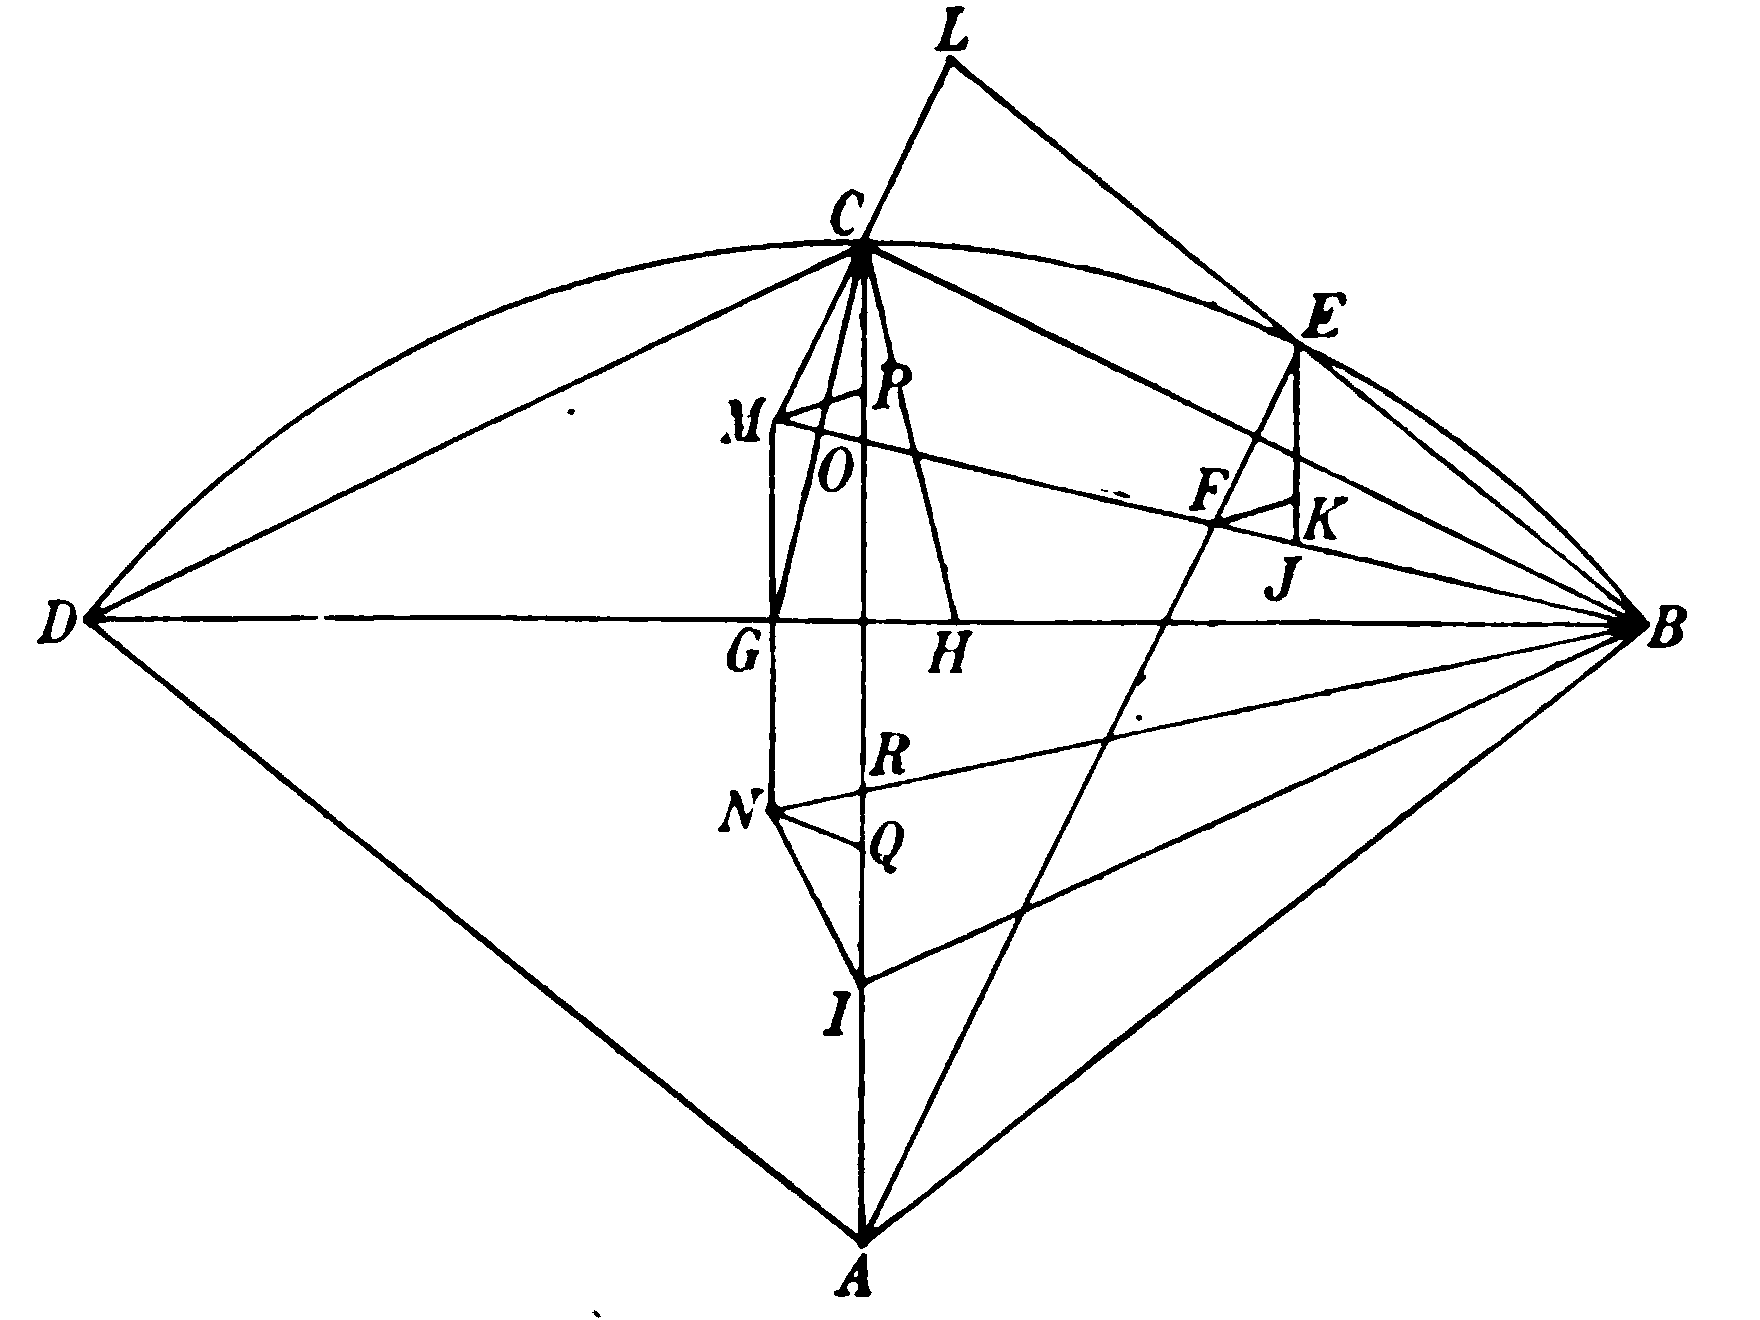
\includegraphics[width=0.56\linewidth]{pdf159-ming-chord-geometry.png}
\end{center}

一八七五年、Tso Ch'ien の \emph{Chui-shu Shih-ming} は、Ming の書の注-
\scanfooter

\scanpage{0160}{第21章、印刷頁146}
釈として、\emph{Pai-fu-t'ang Collections} の一巻に刊行された。Ming 自身の考察による部分と Tso の追加による部分がどれほどかは分からないが、用いられた過程の概要は確かに原論文から取られた。したがって、その書で従われた手続きを見ることにする。まず、円分の弦を弧で表すため、与えられた弧の二分、三分、\ldots{} の弦によってその弦を表す。図で円の半径を一とする。中心が $A$ の円分 $BCD$ で、$C$ を弧の中点、$E$ を弧 $BC$ の中点とする。点 $F$ が直線 $AE$ 上にあるように $BF=BE$ を作る。$BD$ 上に $BG=BC$ および $DH=DC$ を取る。$BC=BG=a$ と書けば $BD=2a-GH$ である。$EJ=EF$ および $FK=FJ$ を引く。$BE$ と $BF$ を延長し、$BL=2\cdot BE$、$BM=2\cdot BF$ とする。$LM$ を結ぶと、明らかに点 $C$ を通る。三角形 $BML$ を辺 $BM$ を軸として回転する。点 $C$ は $G$ に移り、$L$ が移る点を $N$ とする。さらに三角形 $NGB$ を $NB$ を軸として回転すると、点 $G$ は $CA$ 上の一点に移る。それを $I$ とする。明らかに $BI=BC$ である。次に $BM$ が $CA$ と交わる点を $O$ とし、$MP=MO$ を作る。同様に $NQ=NR$ を引く。$R$ は $BN$ と $CA$ の交点である。このような作図を行うと、三角形 $ABE,BEF,FJK,BLM,CMO,MOP,CGH$ はすべて相似であり、二三角形 $CMO$ と $EFJ$ は合同であることが示される。したがって
\[
AB:BE=BE:EF,\qquad AB:EF=BC:GH,
\]
また
\[
1:BE=BE:EF\quad\text{すなわち}\quad EF=BE^2,
\qquad 1:BE^2=a:GH
\]
である。ゆえに $GH=a\cdot BE^2$、したがって $BD=2a-a\cdot BE^2$ を得る。

この基礎の上で考察を進めると、最後に次の式を得る。
\[
BD=2a-\frac{a^3}{4}-\frac{a^5}{4^3}-\frac{2a^7}{4^5}-\frac{5a^9}{4^7}-\frac{14a^{11}}{4^9}-\cdots.
\]

\begin{center}
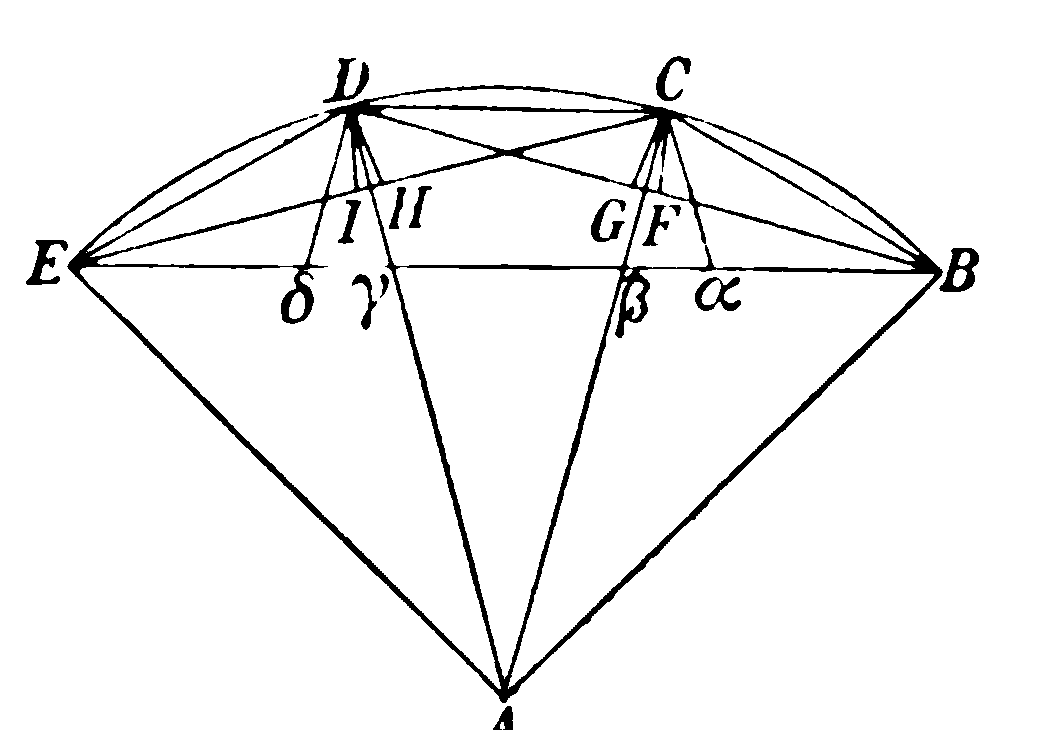
\includegraphics[width=0.38\linewidth]{pdf160-third-part-chord-diagram.png}
\end{center}

次に、弧の三分の一の弦を $a$ と書き、全弧の弦を $a$ によって求めるため、付図のように作図する。ここで $BG,EH$ は $BC$ に等しく作り、$B\delta=E\alpha=BD$、また $\triangle C\alpha\beta\equiv\triangle D\delta\gamma\sim\triangle B\delta D$ 等である。すると
\scanfooter

\scanpage{0161}{第21章、印刷頁147}
\[
AB:BC=BC:CG=CG:GF,\qquad BC:FG=BD:\delta\gamma,
\]
\[
2\cdot BD=BE+\delta\alpha\quad\text{または}\quad 2\cdot BD-\delta\gamma=BE+BC,
\]
\[
\therefore\quad 2\cdot BD-\delta\gamma-BC=BE
\]
となる。これに基づいて進めると、最後に $BE=3a-\frac{4a^3}{4}$ を得る。

与えられた弧の四分の一の弦を $a$ とし、その弧の弦を $a$ で表すとき、同様に
\[
(\mathrm{chord})=4a-\frac{10a^3}{4}+\frac{14a^5}{4^3}-\frac{12a^7}{4^5}+\cdots
\]
を得る。同様の処理によって、与えられた弧の十分の一、百分の一、千分の一、一万分の一の弦を $a$ とすると、弧全体の弦の式はそれぞれ
\[
10a-\frac{165}{4}a^3+\frac{3003}{4^3}a^5-\frac{21450}{4^5}a^7+\cdots,
\]
\[
100a-\frac{166\,650}{4}a^3+\frac{3330\,00030}{4^3}a^5-\frac{31\,63500\,28500}{4^5}a^7+\cdots,
\]
\[
1000a-\frac{1666\,66500}{4}a^3+\frac{3333\,30000\,00300}{4^3}a^5-\cdots,
\]
\[
10000a-\frac{16\,66666\,65000}{4}a^3+\frac{3333\,33300\,00000\,03000}{4^3}a^5-\cdots
\]
となる。最後の三式の $a^3$ の係数を除数とし、それぞれ $100^3,1000^3,10000^3$ を割ると、
\[
24\cdot0024\ldots,
\qquad 24\cdot00002\,4\ldots,
\qquad 24\cdot00000\,024\ldots
\]
を得る。したがって、これらを初項とする数列の項は値二四にますます近づく。ゆえに弧を第一項とすると、弦の式の第二項は $-\frac1{24}(\arcop)^3$ と取るべきである。

同様に $a^5$ の係数と $100^5,1000^5,10000^5$ を用いて前項との比を求めると、
\[
80\cdot07\ldots,
\qquad 80\cdot0007\ldots,
\qquad 80\cdot00000\,7\ldots
\]
を得て、極限値は八〇に近づくと結論される。したがって第三項は
\[
\frac1{24\times80}(\arcop)^5
\]
と取るべきである。
\scanfooter

\scanpage{0162}{第21章、印刷頁148}
同様に第四項は $\frac1{24\cdot80\cdot168}(\arcop)^7$ と求まり、以下同様である。しかし数 $24,80,168,\ldots$ は
\[
24=4(2\cdot3),\qquad 80=4(4\cdot5),\qquad 168=4(6\cdot7),\ldots
\]
の形であるから、最後に弦の公式
\[
(\mathrm{chord})=(\arcop)-\frac{(\arcop)^3}{4\times3!}+\frac{(\arcop)^5}{4^2\times5!}-\frac{(\arcop)^7}{4^3\times7!}+\cdots
\]
を得る。

ここでは不完全帰納法が巧みに適用されていることが分かる。この点は、後章で見る日本の \emph{yenri} 理論の発展に大いに似ている。

次に弦 $c$ によって弧 $a$ を求めるため、今得た級数に級数の逆転を適用する。半径を $m_1$、$c$ の級数を $m_2$ と書き、連比例
\[
m_1:m_2=m_2:m_3=m_3:m_4=m_4:m_5=\cdots
\]
を作ると、計算によって
\[
m_2=a-\frac1{4\times3!}a^3+\frac1{4^2\times5!}a^5-\frac1{4^3\times7!}a^7+\cdots,
\]
\[
m_4=a^3-\frac3{4!}a^5+\cdots,
\qquad
m_6=a^5-\frac5{4\times3!}a^7+\cdots
\]
等を得る。逐次加えると
\[
m_2+\frac{m_4}{3!\cdot4}=a+0-\frac{9a^5}{5!\cdot4^2}+\cdots,
\]
\[
m_2+\frac{m_4}{3!\cdot4}+\frac{9m_6}{5!\cdot4^2}=a+0+0-\frac{228a^7}{7!\cdot4^3}+\cdots,
\]
\[
m_2+\frac{m_4}{3!\cdot4}+\frac{9m_6}{5!\cdot4^2}+\frac{228m_8}{7!\cdot4^3}=a+0+0+0-\cdots,\quad\mathrm{etc.}
\]
となる。したがって操作の終りには
\[
a=m_2+\frac1{3!\cdot4}m_4+\frac9{5!\cdot4^2}m_6+\frac{228}{7!\cdot4^3}m_8+\cdots,
\]
すなわち
\[
a=c+\frac1{3!\cdot4}c^3+\frac9{5!\cdot4^2}c^5+\frac{228}{7!\cdot4^3}c^7+\cdots
\]
を得る。

Tu Tê-mei、すなわち Jartoux の公式のうち、$\sin x$ および $\versin x$ の展開、また $\cos x=1-\versin x$ であるから $\cos x$ の展開は、Europe では James Gregory（一六三八--一六七五年）が一六六七年の \emph{Vera Circuli et Hyperbolae Quadratura} で初めて得た。$\arcop\sin x$ の展開は
\scanfooter

\scanpage{0163}{第21章、印刷頁149}
Sir Isaac Newton が一六七六年の日付を持つ著作で与え、その展開に級数の逆転を適用した。したがって、これらの級数の発明から数年後に China に来た Jartoux は、Frenchman ではあったが、English mathematicians の得た結果を知っていた可能性がある。前述の Ming An-t'u の書で用いられた級数の逆転も、Jartoux を通じて European の資料から学ばれた可能性がある。しかし Newton の方法が Ming の方法と同じであったかは確かでない。両者は詳細な比較を待つ。

Tu Tê-mei の弧の平方の公式は、日本の Takebe Kenkō が一七二二年に与えたものと同じである。しかしその解析法は China の Ming が用いたものと全く異なる。Western World では、この級数は J. de Stainvilles が \emph{Melanges d'Analyse Algebrique et de Géometrie}、p. 460、Paris、一八一五年で刊行した。しかし、それ以前の一七三七年十二月十日、Leonhard Euler が Johann Bernoulli への手紙で与えており、その手紙は G. Eneström により一九〇四年に初めて印刷された。\footnote{P. Harzer、\emph{Die exacten Wissenschaften im alten Japan}、\emph{Jahresbericht der D. M. V.}、第14巻、pp. 318--319。Euler の当該書簡は \emph{Bibliotheca Mathematica}、第3系列、第V巻、p. 270 に掲げられる。} これらの例以外、十八世紀またはそれ以前の Europe にこの級数が存在したか、われわれは全く知らない。

Tu Tê-mei、すなわち Pierre Jartoux が実際にこの級数を有していたなら、自ら得た可能性がある。その場合、彼が才能ある数学者であったと認めなければならない。九公式すべてを先人から学んだのであっても、その知識の深さを同様に賞賛すべきであり、彼が職業的数学者ではなかったことを考えれば、賞賛はさらに増す。いずれにせよ、これらの公式の導入によって中国数学は大いに豊かになった。これらの結果へ至る解析を彼が教え、または Mei Ku-ch'êng がその教えを記録していたなら、中国人は疑いなくさらに多くを得たであろう。

もし実際には Tu Tê-mei が級数を教えず、T. Hayashi の推測どおり Ming An-t'u が初めて立てたのであれば、中国数学史における Ming の功績は高く評価されるべきである。彼の忍耐強い労作が後代の数学者の関心を喚起するのに大いに寄与したことは確かである。いずれにせよ、彼は中国人がこの主題の解析的研究に入った最初の例であった。Ming が研究に成功したのは、Takebe が日本で同じ級数を確立することに成功してからほぼ半世紀後であったが、その確-
\scanfooter

\scanpage{0164}{第21章、印刷頁150}
立において両学者が従った解析法は全く異なっていた。

Yüan Yüan と同時代で、したがって十八世紀末または十九世紀初めに属する Fang Ching-fu も、無限級数の展開に関心を持った。Lo Shih-lin によれば、\footnote{Lo の「Supplements to Biographical Collections」、第48巻。} Fang は Tu Tê-mei の九公式を得て研究した。それが Ming An-t'u の書の刊行前であったなら、\footnote{Ming の著作は一八四〇年に初めて印刷された。} Fang の結果は調査の結果、他方の結果と一致すると分かった。

Ming の半世紀後、Tun Yu-ch'êng（一七九一--一八二三年）が現れた。三巻から成るその著作 \emph{Ko-yüan Lien-pi-li T'u-chieh} は同じ研究系列に属した。Tu Tê-mei の九公式を含む古写本が彼を研究へ駆り立てた。この古写本は一八一九年に Chu Hung から得た。Tun は Tu の公式の導出に説明または解析を与え、さらに四公式を加えた。著作完成後に Ming の書を得たが、彼が見たところ、両数学者の手続きは必ずしも同じではなかった。\footnote{Lo の「Supplements」、第51巻、および Chu の「Third Part」、第2巻。} Tun が得た四公式は次のとおりである。\footnote{Hsü Yu-t'ing の \emph{T'sê-yüan Mi-lu}、第3巻。}
\[
\begin{aligned}
b={}&\frac{a}{n^2}+\frac{(n^2-1)T_1\cdot2T_1}{r\times3\cdot4}
+\frac{(4n^2-1)T_2\cdot2T_1}{r\times5\cdot6}
+\frac{(9n^2-1)T_3\cdot2T_1}{r\times7\cdot8}+\cdots,\\
a={}&n^2b-\frac{(n^2-1)T_1\cdot2b}{r\times3\cdot4}
+\frac{(n^2-4)T_2\cdot2b}{r\times5\cdot6}
-\frac{(n^2-9)T_3\cdot2b}{r\times7\cdot8}+\cdots,\\
b'={}&\frac{a'}n+\frac{(n^2-1)T_3\cdot T_1^2}{r^2\times2\cdot3}
+\frac{(9n^2-1)T_2\cdot T_1^2}{r^2\times4\cdot5}
+\frac{(25n^2-1)T_3\cdot T_1^2}{r^2\times6\cdot7}+\cdots,\\
a'={}&nb-\frac{(n^2-1)T_1b^2}{r^2\times2\cdot3}
+\frac{(n^2-9)T_2b^2}{r^2\times4\cdot5}
-\frac{(n^2-25)T_3b^2}{r^2\times6\cdot7}+\cdots.
\end{aligned}
\]
ここで $a$ は弧（その半分を $x$ と書く）の弦、$b$ はその弧の $n$ 分の一の弦、$a'=\sin x$、$b'=\sin\frac{x}{n}$、$r=$ 半径であり、$T_1,T_2,\ldots$ は第一、第二、\ldots{} 項である。

中国人は十九世紀初めまで楕円の長さを求めようとしなかった。Chu Hung は China でこの問題を取り上げた最初の人物であったことは確かである。一八〇二年に \emph{chin-shih} の学位を得て、一八三〇年に退官するまで官職にあった。
\scanfooter

\scanpage{0165}{第21章、印刷頁151}
その後、数年間 Peking に住んだ。Chu は Tun その他の数学者と親交を結び、彼らと主題を有益に論じた。\footnote{Chu の「Third Part of Biographical Collections」、第2巻。} Chu Hung は、円柱を斜めに切ると楕円が得られることを知り、したがって楕円の計算は直角三角形を用いて行えると考えた。Tun Yu-ch'êng はこれに図式的説明を試みた。円が正方形に似るなら、楕円は長方形に似ると考えた。楕円には長軸、短軸、周長、面積等の量がある。そのうち任意の二つを知れば、他を求められる。Lo Shih-lin によれば、\footnote{Lo の「Supplements」、第51巻。} Tun のこの問題の取扱いは、\emph{Chiu-chang}、すなわち「Nine Sections」で木の幹に巻きつく蔓の長さを計算したのと同じ仕方で行われたらしい。彼が得た公式は
\[
(\mathrm{half\ perimeter})=\sqrt{(a^2-b^2)+\left(\frac12b\pi\right)^2}
\]
であり、$a,b$ は長径と短径の長さである。その不正確さは Lo もすでに認識していた。Tun の研究はさらに高階差の数列、球面三角法、暦学の領域に及んだ。Wang Lai が第 $n$ 項が $n$ の四次式となる数列を先に研究していたとしても、より高次の代数式で表される項を持つ数列を考察することは Tun に残されていた。\footnote{同書。}

Tun とほぼ同時代に、円の解析的考察の研究で名を知られた別の学者がいた。Hsiang Ming-ta（一七九五--一八五〇年）である。球面三角法を研究し、次いで楕円弧の長さを求める主題に取り組んだ。その後、円に関する無限展開について Tun の結果に従ったが、著作 \emph{Hsiao-su Yüan-shih} の完成を見ることなく死去した。後に Tai Hsü が著者の依頼を果たして補完したため、第七巻は Tai が書いた。第六巻で Hsiang は無限級数を用いて楕円周長を表し、また同じ方法を方程式の解法に用いた。一八六〇年、Hsü Yu-t'ing はこの著作を刊行しようとし、版木もほとんどすべて準備されていたが、戦闘で倒れた。そのため刊行は遅れ、
\scanfooter

\scanpage{0166}{第21章、印刷頁152}
著作は完全に失われ、数学界に再び現れることはなかった。\footnote{Chu の「Third Part of Biographical Collections」。}

Hsiang と同時代の Tai Hsü（一八〇五--一八六〇年）は、四巻から成る \emph{Wai-chieh Mi-lu} を著した。同じ頃、Li Shan-lan は \emph{Shih-shih Mong-pi} を、Hsü Yu-t'ing は \emph{T'sê-yüan Mi-lu} および \emph{Ko-yüan Chui-shu} 等を著した。これらはすべて同一または関連する主題を扱う。Hsü の \emph{T'sê-yüan Mi-lu}\footnote{T'ing Ch'u-chung 版 Hsü の著作。}、すなわち「円測の精密公式」は、とりわけ次の公式を含む。
\[
p^2=9d^2\left(1+\frac{1^2}{3\cdot4}+\frac{1^2\cdot2^2}{3\cdot4\cdot5\cdot6}+\frac{1^2\cdot2^2\cdot3^2}{3\cdot4\cdot5\cdot6\cdot7\cdot8}+\cdots\right),
\]
\[
p^3=54q\left(1+\frac{1^2}{3\cdot4}+\frac{1^2\cdot2^2}{3\cdot4\cdot5\cdot6}+\frac{1^2\cdot2^2\cdot3^2}{3\cdot4\cdot5\cdot6\cdot7\cdot8}+\cdots\right).
\]
ここで $p$ は直径 $d$ の円の円周、$q$ は同じ直径を持つ球の体積である。回転楕円体、楕円柱、楕円錐およびその截頭体の体積は、それぞれ
\[
\frac{a^2b}{2},\qquad \frac34abh,\qquad \frac14abh,\qquad
\frac18h\{(2a+a')b+(2a'+a)b'\}
\]
に、
\[
\pi=1+\frac{1^2}{3!\cdot4}+\frac{1^2\cdot3^2}{5!\cdot4^2}+\frac{1^2\cdot3^2\cdot5^2}{7!\cdot4^3}+\cdots
\]
を掛けたものとして与えられる。ここで $a,b$ は長径と短径を表し、$a',b',h$ の意味は明らかである。

Hsü Yu-t'ing は一八〇一年 Wu-chêng に生まれ、一八二九年に \emph{chin-shih} の学位を得た。Taiping Rebellion の間、Chiang-su の軍政長官であった。一八六〇年、帝国軍は Ching-nan で敗れ、viceroy は逃亡した。反乱軍の troups は洪水のように Su Chou へ迫った。Governor Hsü は軍の先頭に立ち勇敢に防衛した。しかし守備隊は四千人に満たず、ほどなく崩れた。Hsü は剣に刺されて倒れ、一家も全員殺された。生前の Hsü は誠実な施政と熱意、職務への忠実さで知られた。著作の一部は生前に自ら刊行したが、未刊のものの多くは死亡時に失われた Hsü は若い頃、得た結果だけを書き留め、用いた解析は記さずに
\scanfooter

\scanpage{0167}{第21章、印刷頁153}
いた。詳細な研究の記録を与えれば後世にさらに有益であるとの忠告を受け、それに従うことを望んだが、長く生きて実行することはできなかった。後半生は多忙で、執筆の余暇がなかったからである。\footnote{Chu の「Third Part of Biographical Collections」、第4巻。}

Hsü の「Measurement of the Sphere」の付録には、楕円周長の公式がいくつかある。Tun の公式はすでに掲げた。Tun の後、Hsiang Ming-ta は長軸を直径とする円の円周と周長差を測ることにより求長を試みた。Tai Hsü も短軸を直径とする円の測定と周長差を用いて同じことを行った。次いで Hsü Yu-t'ing は、本人によれば、より満足できる別の公式を得た。\footnote{Hsü の「Measurement of the Sphere」、付録。Ting の再刊。} Hsü の著作から Hsiang と Tai の公式を掲げる。次のように書く。
\[
\begin{aligned}
K={}&\frac{m}{a}+\frac{1^2\cdot3}{2^2}\frac{m^2}{a^3}
+\frac{1^2\cdot3^2\cdot5}{2^2\cdot3^2}\frac{m^3}{a^5}
+\frac{1^2\cdot3^2\cdot5^2\cdot7}{2^2\cdot3^2\cdot4^2}\frac{m^4}{a^7}+\cdots,\\
K'={}&\frac{m}{b}-\frac{1^2\cdot3}{2^2}\frac{m^2}{b^3}
-\frac{1^2\cdot3^2\cdot5}{2^2\cdot3^2}\frac{m^3}{b^5}
-\frac{1^2\cdot3^2\cdot5^2\cdot7}{2^2\cdot3^2\cdot4^2}\frac{m^4}{b^7}-\cdots.
\end{aligned}
\]
ここで $a,b$ は長径と短径、$m=\frac14(a^2-b^2)$ であり、楕円周長は $K\pi a$ および $K'\pi b$ によって表される。Hsü 自身の公式は、楕円と等周の円の円周を求める形で表された。これらの公式がどのような過程または解析で計算されたかを説明する資料がないのは、非常に残念である。

以下では、弦から円分の高さを計算する Hsü の過程について若干述べる。\footnote{Hsü の \emph{Ko-yüan Chui-shu}、すなわち「Analysis of Circle-Measurement」第2巻。Wu Chia-shan が注釈し、Tso Ch'ien が補い、Ting が一八七四年に刊行。} 説明すべき公式は $\versin x=T_1+T_2+T_3+\cdots$ で、逐次項は
\[
T_1=\frac{\sin^2x}{d},\qquad
T_2=\frac{T_1^2}{d},\qquad
T_3=\frac{(2T_1+T_2)T_2}{d},\qquad
T_4=\frac{[2(T_1+T_2)+T_3]T_3}{d},\ldots
\]
の形である。この式を導くため、付図から考察を始める。長方形は次のように構成される。
\scanfooter

\scanpage{0168}{第21章、印刷頁154}
$EK=$ 矢、$KA=$ 補矢、すなわち直径と与えられた矢との差であり、$KC$ は $KE$ に等しい。

\begin{center}
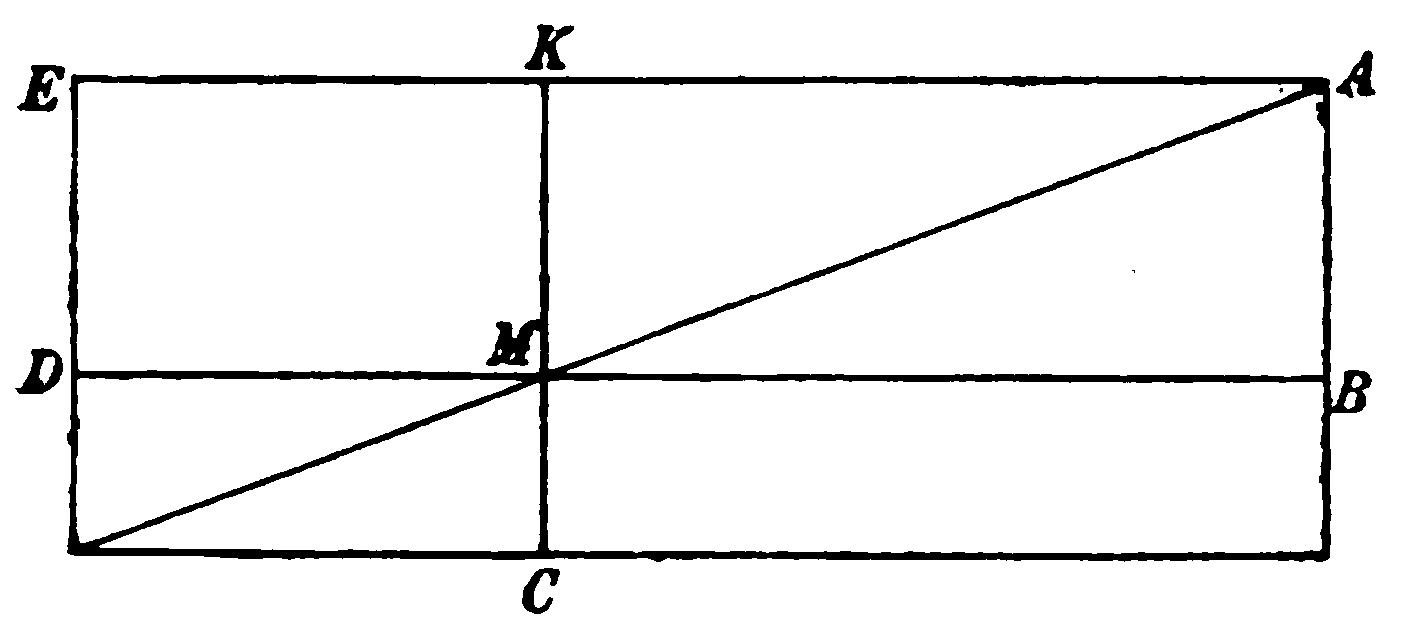
\includegraphics[width=0.50\linewidth]{pdf168-rectangle-derivation-1.png}
\end{center}

ここで長方形 $AC$ は、矢と補矢の積、すなわち $\sin^2x$ に等しい。しかし $\rectsym AC=\rectsym AD$ であるから、$\therefore\ \rectsym AD=\sin^2x$ である。したがって直径 $d$ で割ると、$T_1$ と書く長さ $ED$ を得る。ゆえに $T_1=\sin^2x/d$ である。

次に付図のように構成すると、$\rectsym KN=\rectsym NH=\rectsym BG$ である。しかし $\rectsym KN=T_1T_1$ であるから、$T_1T_1/d=DG=T_2$ と書く。

\begin{center}
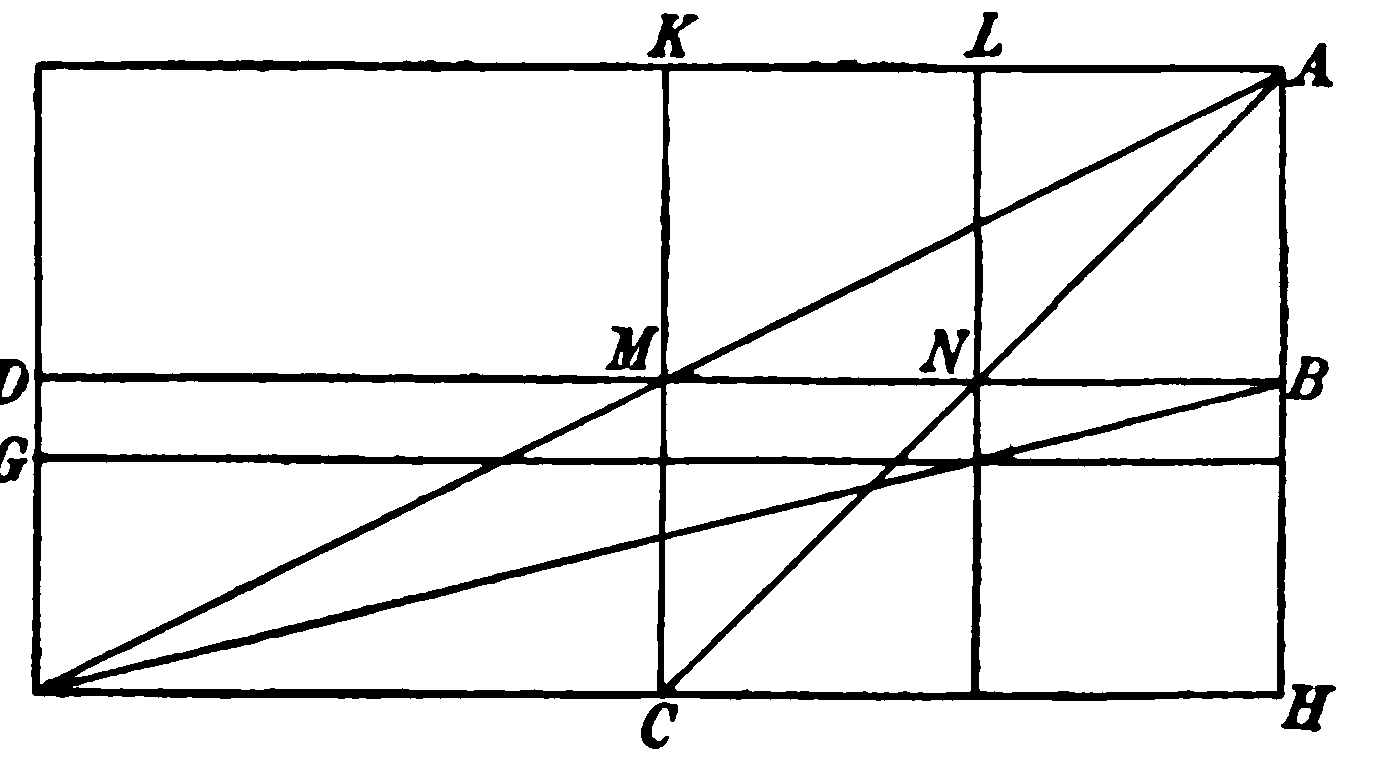
\includegraphics[width=0.52\linewidth]{pdf168-rectangle-derivation-2.png}
\end{center}

次に、斜線部が正方形となるようにした付図を描くと、$\rectsym LN'=(T_1+T_2)T_2=\rectsym DG'$ である。ここで $G'$ は $MD'=N'H'$ となるように取る。また $\rectsym MM'=T_2T_1$ であるから、$\therefore\ \rectsym DG'+\rectsym MM'=(2T_1+T_2)T_2$ である。さらに $\rectsym DM'=\rectsym M'H$ であるから、$(2T_1+T_2)T_2=\rectsym N'H=\rectsym B'G''$、したがって
\[
T_3=\frac{(2T_1+T_2)T_2}{d}=GG''
\]
である。

\begin{center}
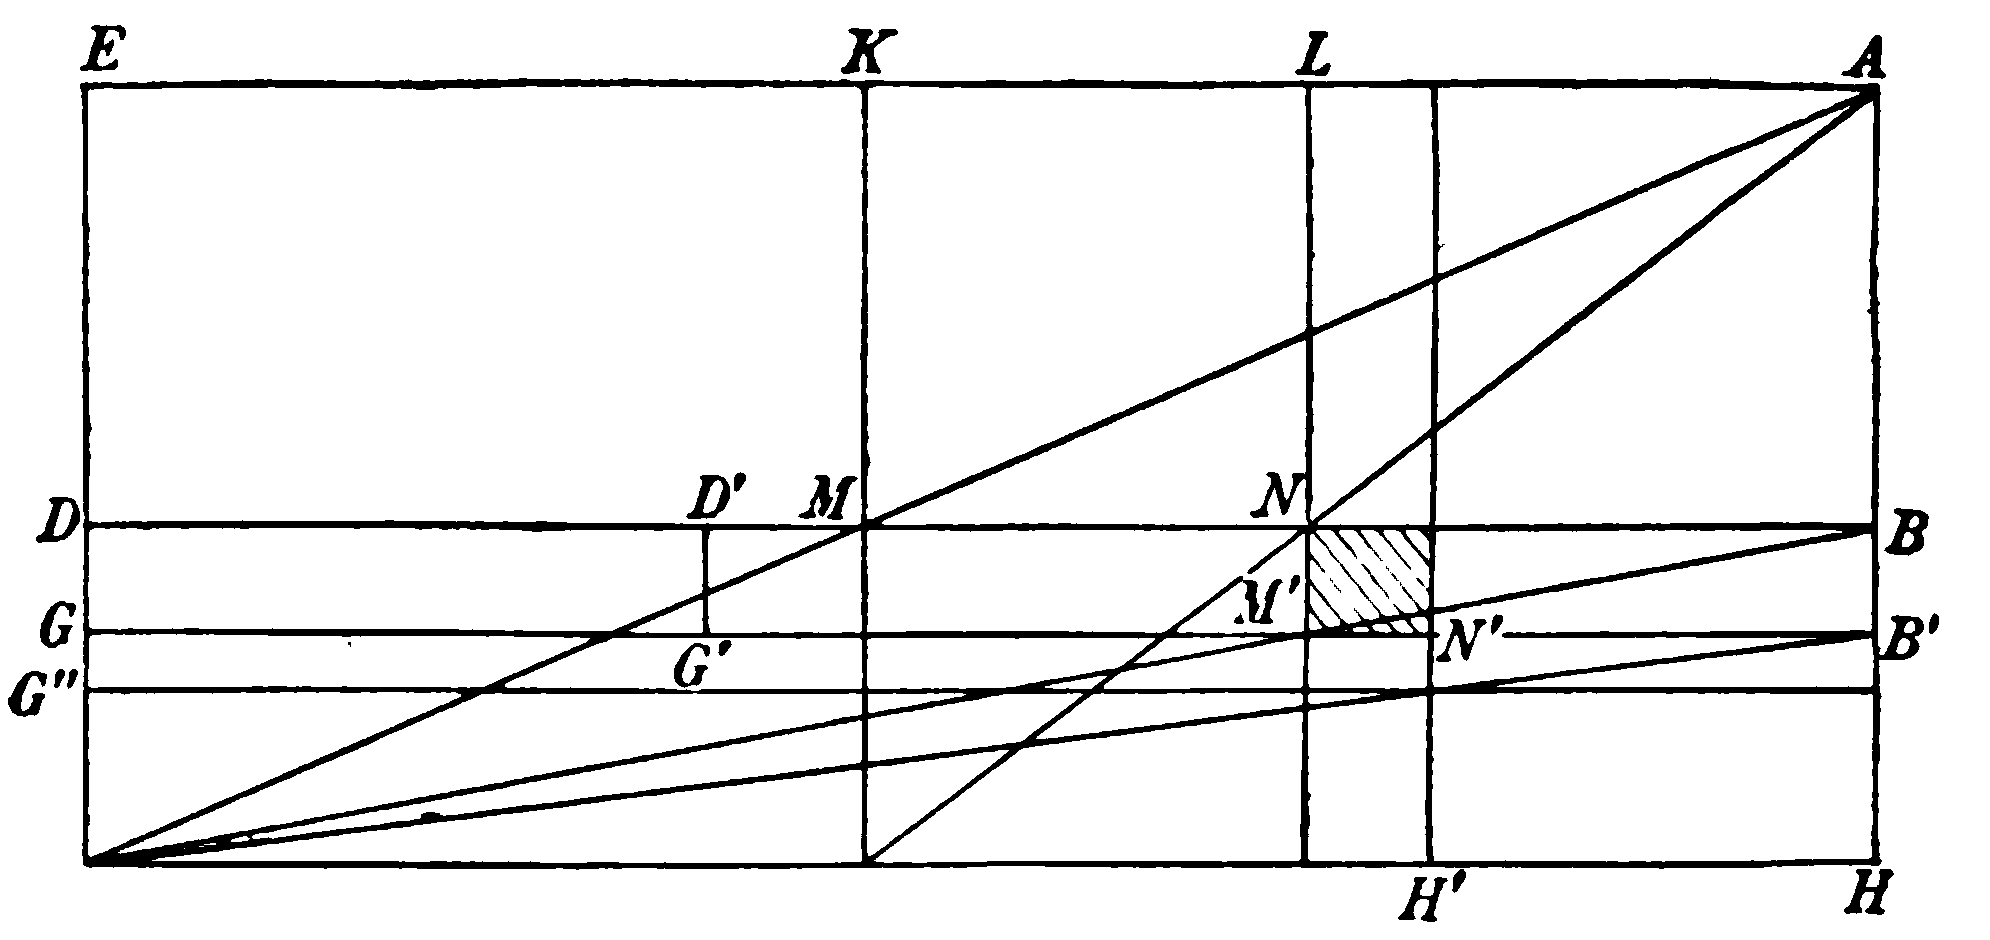
\includegraphics[width=0.58\linewidth]{pdf168-rectangle-derivation-3.png}
\end{center}

このようにして前述の展開を得ることができる。しかし Hsü はさらにこれを変形する。次の比例が成り立つ。
\[
\begin{array}{rcl}
(1)&d:\sin x&=\sin x:T_1,\\
(2)&d:T_1&=T_1:T_2,\\
(3)&d:T_2&=2T_1+T_2:T_3,\\
(4)&d:T_3&=2(T_1+T_2)+T_3:T_4,\ldots.
\end{array}
\]
\scanfooter

\scanpage{0169}{第21章結尾、印刷頁155}
いま $m_1=r$、すなわち半径、$m_2=\sin x$ と書き、連比例
\[
m_1:m_2=m_2:m_3=m_3:m_4=m_4:m_5=\cdots
\]
を作る。これは $m_k=\sin^{k-1}x/r^{k-2}$ と取ることを意味する。この記法を用いると、上の比例から\footnote{原著では比例を付図の形で表す。各項は右から左へ数える。
\[
\begin{array}{|c|c|c|c|}
\hline
d&c&b&a\\
\hline
\end{array}
\]}
\[
(1)\quad 2m_1:m_2=m_2:\frac{m_3}{2},
\qquad
(2)\quad 2m_1:\frac{m_3}{2}=\frac{m_3}{2}:\frac{m_5}{2\cdot4}
\]
を得る。公式 (3) は二つの比例に分けて考える。\footnote{これらの比例は原著では付図のように示される。
\[
\begin{array}{|c|c|c|c|}
\hline
\dfrac{2m_7}{2\cdot4^2}&\dfrac{2m_3}{2}&\dfrac{m_5}{2\cdot4}&2m_1\\
\hline
\dfrac{m_9}{2\cdot4^3}&\dfrac{m_5}{2\cdot4}&\dfrac{m_5}{2\cdot4}&2m_1\\
\hline
\end{array}
\]}
\[
2m_1:\frac{m_5}{2\cdot4}=\frac{2m_3}{2}:\frac{2m_7}{2\cdot4^2}
\quad\text{および}\quad
2m_1:\frac{m_5}{2\cdot4}=\frac{m_5}{2\cdot4}:\frac{m_9}{2\cdot4^3}.
\]
二つの第四比例項を加えて $T_3$ を得る。すなわち
\[
T_3=\frac{2m_7}{2\cdot4^2}+\frac{m_9}{2\cdot4^3}.
\]
同様に $T_4,T_5$ は
\[
T_4=\frac{4m_9}{2\cdot4^3}+\frac{6m_{11}}{2\cdot4^4},
\qquad
T_5=\frac{8m_{11}}{2\cdot4^4}
\]
と得られ、$m_{13}$ 以後の項は捨てる。これらを加えると $T_1+T_2+T_3+\cdots$ は
\[
\frac{m_3}{2}+\frac{m_5}{2\cdot4}+\frac{2m_7}{2\cdot4^2}+\frac{5m_9}{2\cdot4^3}+\frac{14m_{11}}{2\cdot4^4}+\cdots
\]
に等しい。これは公式
\[
\mathop{\mathrm{ver\,sin}}x
=\frac12\frac{\sin^2x}{r}
+\frac1{2\cdot4}\frac{\sin^4x}{r^3}
+\frac2{2\cdot4^2}\frac{\sin^6x}{r^5}
+\frac5{2\cdot4^3}\frac{\sin^8x}{r^7}+\cdots
\]
を取ることと同じである。
\scanfooter


\scanpage{0170}{第二部および第22章冒頭、印刷頁156}
\begin{center}
第二部。\\[1mm]
日本数学。\\[3mm]
第22章。\\[1mm]
日本数学の概観。
\end{center}
\phantomsection\addcontentsline{toc}{section}{第II部　日本の数学}
\phantomsection\addcontentsline{toc}{subsection}{第22章　日本数学の概観}

最古の時代に日本人が有していた数学的知識について、われわれは実際上何も知らない。六世紀に Korea を経て Buddhism が伝来した後、中国数学の一部が Japan にもたらされ、しばらくの間、土着の学者によって研究された。しかし彼らの知識はきわめて限られていたに違いない。自立して研究を進めるところまで、彼らは一度も到達しなかったからである。彼らにできたことは、中国の師に盲目的に従うことだけであった。このような卑しい状態さえ長くは続かず、政治的規制が緩むと学問も同じ運命を分かち、次第に衰退して、ついには実際上何も残らなくなった。

日本人が数学研究を真に重視するようになったのは、中国数学が再び導入された後であった。長い暗黒時代を経て、十七世紀に至って学問はようやく再度好意をもって受け入れられ、さまざまな学者が現れた。その手によって、いわゆる固有の日本数学は夜明けを迎え、その後二世紀以上にわたって栄える運命にあった。

歴史上最初に名を留める日本人数学者は、十七世紀初頭に生きた Mōri Kambei である。彼は China に渡ったことがあると時に記されるが、その話は確実に真正とはいえない。

中国の算盤 \emph{suan-pan} は、日本人が \emph{soroban} と呼ぶものであり、Mōri の時代以来、Japan で広く用いられてきた。通説では Mōri が China から初めて持ち帰ったとされるが、その導入はさらに古いように思われる。いずれにせよ Mōri は、この器具を扱う技術に熟達していた。彼が Kyōto で \emph{soroban} 算術を教えると、多数の門人が彼のもとに集まった。算盤の普及において Mōri が少なからぬ役割を果たしたことは確かである。Mōri は \emph{soroban} の使用に関する書物を刊行したといわれるが、それは後に失われた。
\scanfooter

\scanpage{0171}{第22章、印刷頁157}
Mōri の多数の門人のうち、とりわけ傑出した三人がいた。Yoshida Kōyū、Imamura Chishō、Takahara Kisshū である。\emph{Sanshi}、すなわち「三人の尊敬すべき数学者または学者」という呼称は、同時代人が敬意をこめて彼らに与えたものであった。

Yoshida の一六二七年の \emph{Jinkōki} は成功した出版物であった。その出現後、\emph{soroban} 算術は急速に進歩した。同書は非常な人気を得る運命にあり、著名な著者の存命中にさえさまざまな版を重ねた。書肆が著者の知識も許可もなくこれを重刊することもあった。後代には、同じ表題に何らかの接頭語を加えた書物が数十種も刊行された。

Yoshida の著作にはさまざまな出版物が続き、それらも同書と同様、主として一五九三年の中国の Ch'êng Tai-wei の \emph{Suan-fa T'ung-tsung} の内容に基づいていた。この中国の師の著作は一六七五年に Japan で重刊された。

十七世紀前半は、\emph{soroban} 上で実行される算術が国内各地に普及しつつあった、日本数学の一時期であった。しかし今や、学問の進歩に別の刺激が現れた。それは一二九九年の Chu Shih-chieh の \emph{Suan-hsiao Chi-mêng} という、別の中国書の導入であった。Chu の著作については第十四章で述べた。この書は China では長く失われていたが、一六六〇年の Korean 版が発見されて復元され、一八三九年に Lo Shih-lin によって重刊された。博学な Yüan Yüan でさえ、歴史研究の時点では同書を見出すことができなかった。
\footnote{彼の「Biographical Collections」は一七九九年に完成した。}
China では失われていたこの著作は、おそらく一六六〇年に一度重刊された Korea から導入され、Japan で見出されるという幸運な運命を有した。しかし日本人はその年以前から同書を知っていた。日本初版が一六五八年に出ているからである。同書は十七世紀の日本人数学者によって広く研究され、Japan で \emph{sangi} と呼ばれるようになった算木によって操作する器械的代数の初歩を彼らに与えた。これは、いわゆる \emph{t'ien-yuen-shu}、すなわち日本の \emph{tengen jutsu} であり、文字どおり「天元法」を意味する。

\emph{sangi}、すなわち算木は新しい便法ではなかった。China におけるその使用にはすでに言及した。中国数学が Korea から Japan へ最初に導入された際、これらの
\scanfooter

\scanpage{0172}{第22章、印刷頁158}
算木も疑いなく伝来し、それ以来ずっと用いられてきた。しかし \emph{soroban} が普及すると、算木は急速に後退した。新種の算盤に比べてはるかに扱いにくく、実用的でなかったからである。天元法の代数が研究されるようにならなかったならば、算木はほどなく完全に忘却へ沈んだであろう。しかし実際はそうならなかった。\emph{soroban} は日常生活の実務に適していたのに対し、算木は複雑な問題の論究に最も適し、任意次数の数値方程式の解法に適用できた。こうして二種の算盤、\emph{soroban} と \emph{sangi} は並行して栄えることとなった。いずれも旧日本数学派が隆盛した全時代を通じて実践された。

一六二七年に Yoshida の \emph{Jinkō-ki} が現れて以来、数学研究は不断に進歩していたが、天元法の導入は学者の知識を著しく高め、日本人が独立した研究へ踏み出すまでに長い時間はかからなかった。

十三、十四世紀の中国人数学者は天元代数を研究したが、方程式の次数がいかなるものであっても一つの解だけで満足し、一つの方程式に複数の根が存在することを発見するには至らなかった。しかし日本人は、方程式の根が必ずしも一個に限られないことをまもなく見出した。Satō Seikō（一六六六）は、根の多重性から生じる一問題の複数の解を採用した。これに対して Sawaguchi Kazuyuki（一六七〇）は、そのような手続の緩さを攻撃した。ただし彼自身も、ある条件のもとでは複数の解が存在することを認めていた。彼は、そのような解が生じる原因を、問題のデータを構成する量の不適切さに帰した。そこで、データ中に現れる定数の一部を変更し、一つの解だけを生じるようにすることを選んだ。

これらの学者の著作が刊行されて間もなく、日本の Newton と呼ばれる偉大な天才が現れた。その名は Seki Kōwa である。Seki は Galileo が没し Newton が生まれたのと同じ年、すなわち一六四二年に生まれた。Seki がその業績において Newton を凌がなかったとしても、両者に劣るものではなかった。Newton が自国の数学にもたらしたのと同じ高揚を、Seki も Japan に与えることができた。いわゆる固有の日本数学は、その確固たる確立のために彼の天才を待っていたのである。疑いなく Seki は日本数学の父であった。
\scanfooter

\scanpage{0173}{第22章、印刷頁159}
Seki は生涯に多数の写本著作を書いたといわれるが、それらの写本のうち現在残るものはあまり多くない。彼自身の筆になる著作について何も知られていないことは、認めざるを得ない大きな不幸である。しかし、なお保存される少数の著作だけでも、彼の記憶を不朽にするに十分である。彼が第一級の数学者であったことを、誰が否定できようか。

Seki は多くを書いたが、ほとんど印刷しなかった。一六七四年に現れた \emph{Hatsubi Sampō} という一冊を除き、彼は著作を刊行しなかった。しかし同書の出現は、彼にふさわしい名声をもたらす契機となった。

\emph{Jinkōki} の後版で Yoshida は巻末にいくつかの数学問題を掲げ、後継者にその解決を求めた。Isomura は一六六〇年の \emph{Ketsugishō} でこれらの問題を解き、自著の末尾に別の問題を発表した。今度はそれらが、数年のうちに刊行された後続の著作で解かれた。このようにして、新しい問題を提起し、それを後続の出版物で解く慣行が生じ、一世紀半にわたって続いた。この慣行は \emph{idai shōtō}、すなわち「継続的な出題と解答」として知られた。それは数学研究の進歩を少なからず刺激した。すでに触れた Satō（一六六六）および Sawaguchi（一六七〇）の著作も、他のものとともにこの系列の出版物であった。Sawaguchi は十五の新問題を提出し、それに答えたのが Seki の著作であった。Seki の解答の一つは、一四五八次方程式に至った。そのような方程式がいかに途方もないものであったかは、記述するより想像する方がよい。Seki は、確かに方程式そのものを示さないが、その存在を明記している。二十年ほど後、Miyagi Seikō は一六九五年刊の \emph{Wakan Sampō} を著し、同じ問題を考察して、Seki が言及した一四五八次方程式に至る詳細な解析を示した。驚くほど高い次数の方程式を考察することは、十七、十八世紀の日本人数学者には珍しくなかった。次数三千または四千の方程式が考慮されることもあった。次数がいかに高くても、日本人は一貫して天元法を適用して解いた。こうした巨大な方程式を解く際、通常の紙または木製の盤では \emph{sangi} を配置するには小さすぎたため、ある数学者は書斎または座敷の畳全体に罫を引いた \emph{sangi}-board を作り、その上に小さな算木を並べて
\scanfooter

\scanpage{0174}{第22章、印刷頁160}
方程式を解いたという。忍耐と苦学は、旧時代の日本人数学者を特徴づけた精神の一部であった。

Seki が刊行著作を記す際に用いた数学的方法は、彼が \emph{yendan jutsu} と呼んだものであり、文字どおり「説明または解析の方法」を意味する。それは中国の天元代数を拡張したものであり、彼が名高い生涯のうちに築いた巨大な建造物の最初の礎石となった。刊行著作では方法の性質を説明せず、計算結果を方程式の形で示すだけであったとしても、その結果を表現した優美さは、同時代人のあいだで彼の名声を高めずにはいなかった。十数年後、門人 Takebe Kenkō が同書の詳細な解析を試み、そこでこの方法は彼の学派の外の数学界にも一般に知られるようになった。

\emph{yendan} 代数を確立した後、Seki はさらに研究を進め、\emph{tenzan jutsu} の名で知られる誇るべき日本数学体系へ到達することができた。この名称は Seki 自身が用いたものではない。彼はこれを \emph{kigen-seihō} と呼んだが、それはおそらく「埋もれた根源または物の関係を明らかにする方法ないし術」を意味する意図であった。このような語を用いたこと自体、彼が成功をいかに誇りとしていたかを示すに十分である。Seki の \emph{kigen-seihō} は筆算形式の代数体系であった。

\emph{tenzan jutsu} という名称は、Seki の発明から半世紀後、Matsunaga が、仕えていた主君 Naitō Masaki、すなわち Kyūshū の Nobeoka の封建領主の希望を満たすために採用した。Naitō 自身も数学者であった。\emph{tenzan} という語は、「取り去る」を意味する \emph{ten} と「取り入れる」を意味する \emph{zan} の二つの表意文字から成る。したがって、この語の構成は algebra という語の Arabian 起源とよく似ており、実質的に代数にほかならないものの性質を示すきわめて適切な術語であった。しかし西洋の algebra が導入されると、旧語 \emph{tenzan} は新語 \emph{daisū gaku} に譲った。これは中国人が用いた名称をそのまま採用したものであり、文字どおり「数の代わりに文字を用いる学問」を意味する。

Seki の \emph{yendan} 代数は早くから公に知られたが、\emph{tenzan} 体系は秘密に保たれた。一七六九年になって初めて、この方法は印刷著作で扱われた。すなわち Kyūshū の Kurume の大名 Lord Arima が、Toyota という仮名のもとに \emph{Shūki Sampō} を刊行したのである。
\scanfooter

\scanpage{0175}{第22章、印刷頁161}
発明を秘密に保つ慣行は、学問の進歩をかなり遅らせたに違いない。秘密の主題を伝授された者が、常にその時代の最良の精神であったわけでも、そうあり得たわけでもないからである。不幸にも既得権益の精神が学者の行動を支配した。

Seki がともに確立した \emph{yendan} と \emph{tenzan} の二主題はいずれも代数的考察に関わるが、一方は早く刊行され、他方はほぼ一世紀にわたり秘密に留まる運命を負った。旧数学者は明らかにこの二学問の区別を重視していた。そうでなければ、どうしてこれほど異なる扱いが生じたであろうか。しかし旧日本数学派の訓練を受けていないわれわれには、この区別は、少なくとも一見したところ、きわめて曖昧で根拠がないように思われる。それでも日本の学問を深く研究すると、少なくとも一部は明らかになる。\emph{yendan} は問題の説明または解析を意味する意図であった。問題を解くには、まずデータに与えられたさまざまな量の間に存在する関係を考え、所望の解を得るため、すなわち一つまたは複数の解が得られる方程式に到達するまで、計算と工夫を適切に用いなければならない。これらの考察はすべて、\emph{yendan jutsu}、すなわち「説明過程」と呼ばれたものに属する。したがって、これらの段階が算術的に、幾何学的に、筆算代数的に、または算木によって配置された天元法として進められるかを問わず、常に適用できた。後代には \emph{yendan} という語が、明確に「説明」を意味する別語 \emph{kaigi} に置き換えられた。しかし、より限定された厳密な意味では、少なくとも成立当初には、それぞれ通常の単純な天元法の適用によって得られる二つ以上の関係を構成し、そこから天元についての最終方程式を導くことを表したように思われる。したがって T. Endō が正しく理解したように、\emph{yendan} 過程は天元法の通常の代数的取扱いを反復適用するものであった。\emph{yendan} 代数の最終目標は、算木で解くべき数値方程式を構成することにあった。\emph{yendan} 代数は筆算で実行された。

\emph{tenzan} 法の代数では、すべての考察が筆算で行われた。それが \emph{yendan} 代数と本質的に異なる点は、最終結果へ至る解析も利用可能な知-
\scanfooter

\scanpage{0176}{第22章、印刷頁162}
識の一部を構成すると考えられ、全体が筆記されるべきであったことである。ただし最終方程式には、解法として天元法が適用されることもあった。\emph{tenzan} 代数という共通標題のもとで研究された主題は広範であり、方程式論、不定方程式の解法、幾何学的関係の代数的取扱いなどを含んだ。

\emph{yendan} および \emph{tenzan} 代数で用いられた代数記号は、十三、十四世紀の中国人数学者が採用したものと同じであった。それらは実際、今日われわれが用いるものより煩瑣で不便である。十七世紀後半、Seki Kōwa が代数学の確立に活発に従事していた状況を考え、Seki と同時代人が中国の師から借用した記号を思い合わせると、この仕事の過程で日本人が Western World から何かを借りたのではない、という結論へ導かれる。\emph{tenzan jutsu}、すなわち日本の代数は、日本人の精神によって真正に明るみに出されたに違いない。
\footnote{Y. Mikami, \emph{Hatono Sōha and the mathematics of Seki}, \emph{Nieuw Archief voor Wiskunde}, IX, 2 を参照。}

すでに述べたように、Seki の先人たちは方程式の根の多重性を確信していたが、Seki は方程式論をはるかに進めた。彼は、方程式の根が正のものに限られないこと、一般に方程式はその次数と同数の根を有すること、この最大数の根が現れない方程式があること、その場合、存在する根の数は次数より偶数だけ少ないこと、正負いずれの根も持たない方程式があること、未知数の偶数冪だけを含む方程式は、その平方を新たな未知数に取ることで簡略化できること、新しい未知数を取ることで方程式を便利に変換できること、等々を知っていた。また Seki は、問題のデータが時に不足または不可能性へ導くこと、その場合、ある定数の限界を定めて問題を十分または可能にできること、問題のデータから構成した方程式から得た解が、時にその要求を満たさないことも知っていた。
\footnote{これらの結果は Seki の写本 \emph{Kaihō Hompen}, \emph{Byōdai Meichi}, \emph{Daijutsu Bengi}, \emph{Kaihō Sanshiki} などに記録されている。}
\scanfooter

\scanpage{0177}{第22章、印刷頁163}
Seki は導関数を用いるのと同じ規則を与えている。しかし一部の学者が考えるように、彼がその規則を極大・極小の研究へ適用したとは思われない。その適用は後継者に残された。

Seki 以前、算木による方程式の解法は一桁ずつ計算され、労力を省く方法は一度も試みられなかった。China または Japan で初めてこのような省略を試みたのは、われわれの知る限り Seki であった。
\footnote{Seki の \emph{Kaihō Sanshiki} など。}
Seki が行列式の観念を用いたことは非常に注目すべきである。この主題の詳細は第二十四章で説明する。

一般に Seki の発明と信じられている \emph{shōsa} 法、\emph{jōichi} 法などは、確かに彼が中国数学から学んだものであった。\emph{shōsa}、すなわち中国語の \emph{ch'ao-cha} は、いくつかの既知の $x$ の値に対する $S$ の値が分かっているという条件のもとで、未定乗数 $\alpha,\beta,\gamma,\ldots$ を関係
\[
S=\alpha x+\beta x^2+\gamma x^3+\cdots
\]
から決定する方法である。T. Hayashi は \emph{shōsa} 法が European の有限差分法と同一であると考えるが、それはおそらく正しい。Seki はこれを Kuo Shou-ching の著作から学んだ可能性が最も高い。\emph{jōichi jutsu} は、Ch'in Chiu-shao による不定関係
\[
p\alpha-q\beta=1
\]
の解法と同じである。Seki は Ch'in の著作を知っていたのかもしれない。
\footnote{Ch'in の著作については第十一章を参照。}

十七世紀の日本数学が中国の学問の影響を受けていたことは否定できない。しかし Japan で研究されたことが知られる中国書は多くない。一五九三年の Ch'êng Tai-wei の \emph{Suan-fa T'ung-tsung}、Chu Shih-chieh の \emph{Suan-hsiao Chi-mêng}、Kuo Shou-ching の暦学著作が、われわれの知る限り Japan にもたらされたもののほぼすべてであった。十八世紀初頭には Mei Wen-ting の \emph{Li-suan Ch'üan-shu}、一七一三年の \emph{Su-li Ching-yün} などが輸入された。Seki の門人 Takebe は Mei の著作を研究して注記を書き、Takebe の門人 Nakane Genkei はその一部を翻訳した。三角法はこれらの著作を通じて西洋の源泉から Japan に導入された。対数も China から日本人にもたらされた。しかし西洋数学が Land of the Rising Sun の学問へ及ぼした実質的影響について、われわれは何も知らない。

日本数学の最高の発達は、当然 \emph{yenri}、文字どおり
\scanfooter

\scanpage{0178}{第22章、印刷頁164}
「円の原理」または「円理」の発明に求めなければならない。それは解析的考察によって行う円の測定であった。この方法はさまざまな発展段階を経たが、伝わっている最初の例は Takebe、Tanzan（または Awayama）らが記録したものである。Takebe の写本 \emph{Yenri Tetsujutsu} または \emph{Yenri Kōhaijutsu} の初歩は次のとおりである。
\footnote{この写本の詳しい説明は D. Kikuchi の論文 \emph{Seki's method of finding the length of an arc of a circle}, \emph{Proceedings of the Tokyo M. P. S.}, vol. 8, pp. 179--198 にある。Smith and Mikami, \emph{A History of Japanese Mathematics}, Chicago も参照。}

円弧形に、辺数 $2,2^2,2^3,\ldots$ の正多角線を順次内接させる。二角線の一辺に対する矢は、関係
\[
-ds+4dx-4x^2=0
\]
から得られる。ここで $d$ は直径、$s$ は与えられた弧の矢、すなわち高さである。この方程式の一根は、\emph{tetsujutsu} と呼ばれる数学的方法によって二項級数へ展開できる。同じ展開法を $2^2$ 角線の一辺の矢へ適用でき、その際、二角線の矢の展開形を用いる。この操作は任意回繰り返せる。しかしこの手続は実行不能であるため、Takebe はこの方法で $2,2^2,2^3,2^4$ 角線の矢を最初の十項または六項まで展開するにとどめ、係数を比較して、それらを支配する関係を不完全帰納によって立て、$2^{10}$ 辺までの多角線の矢の表を作った。$2^i$ 角線の矢と直径との積は、$2^{i+1}$ 角線の一辺の平方である。その結果に $\left(\frac12\times2^{i+1}\right)^2$ を乗じると、内接 $2^{i+1}$ 角線の長さの半分の平方を得る。この量の表も作られ、そこから
\[
\lim_{n=\infty}\left\{\frac12\times(\text{$2^n$ 角線の長さ})\right\}^{2}
\]
の値が不完全帰納によって導かれる。その結果は級数
\[
\frac14(\mathrm{arc})^2
=ds\left\{1+\frac{2^2}{3\cdot4}\left(\frac{s}{d}\right)
+\frac{2^2\cdot4^2}{3\cdot4\cdot5\cdot6}\left(\frac{s}{d}\right)^2
+\frac{2^2\cdot4^2\cdot6^2}{3\cdot4\cdot5\cdot6\cdot7\cdot8}\left(\frac{s}{d}\right)^3+\cdots\right\}
\]
である。この級数が Tu Tê-mei、すなわち French の Pierre Jartoux の、いわゆる九公式の一つと同じであることに気づくであろう。（第二十一章参照。）

今述べた解析による円測は通常 Seki に帰されるが、これはあまり
\scanfooter

\scanpage{0179}{第22章、印刷頁165}
真正とは思われない。\footnote{Y. Mikami, \emph{A question on Seki's invention of the circle-principle}, Proc. of Tokyo M. P. S., 2nd Series, vol. 4.}
古い写本（Tanzan Shōkei の一七二八年の \emph{Yenri Hakki}）によれば、この解析または結果の級数は、Takebe が数十年にわたって研究を続けた後、一七二二年に得たものである。

いずれにせよ、Seki が円測の主題に大きく貢献したことは確かである。彼は当然、歴史に語るに値するさまざまな成果を得た。Ōtaka の \emph{Kwatsuyō Sampō} は、一七〇九年に Seki の著作から編纂され、一七一二年に刊行されたもので、Seki の成果の一部を収めている。第四巻には円測に関する事項がある。Seki が円弧の平方を決定するために与えた公式は、直径と矢について七次である。この公式は、ある既知の弧の数値から導かれたように思われる。この主題については第二十八章で述べる。

円弧の数値を計算する際、Seki は当然、内接二角線から始めて辺数を順次二倍する数値的工夫を用いる。これは円積法で用いられるのと同じ方法である。
\footnote{$\pi$ の値については第二十五章を参照。$\pi$ および $\pi^2$ のさまざまな級数は第二十九章に掲げる。}
この種の円測は彼以前から存在したが、なお彼が完成すべき一事が残っていた。それは、このように数値計算した結果の補正であった。$a,b,c$ を内接多角形または多角線の周長の連続する三つの値とすれば、補正値は
\[
b+\frac{(b-a)\times(c-b)}{(b-a)-(c-b)}
\]
となる。後の注釈から分かるところでは、この補正は連続値の差を無限等比級数と比較することによって試みられた。

この補正法は任意回適用できるが、Seki 自身はそうしなかった。反復補正を適用したのは門人 Takebe であった。Takebe の小数点以下四十一桁まで正しい $\pi$ の値は、この方法で計算された。同様の仕方で円弧平方の値を多数桁まで計算し、彼はまた不完全帰納によって円弧平方の級数を導いた。同様な推論によって、同じ量についてさらに二つの級数を与えた。これらの成果は一七二二年の \emph{Fukyū Tetsujutsu} に収められている。
\footnote{Smith and Mikami, \emph{History} を参照。}
\scanfooter

\scanpage{0180}{第22章、印刷頁166}
Takebe の円理研究には Matsunaga の研究が続いた。彼の一七三九年の \emph{Hōyen Sankyō} は、円、その平方、円弧、その平方、円弧形の高さ、およびその弦について八つの級数を含む。
\footnote{これらの級数については Smith and Mikami の \emph{History} を参照。}
その一つは Takebe の級数と同じで、他の三つは Mei Ku-ch'êng の「Pearls dropped in the Red River」に見られる。
\footnote{第二十一章参照。}
Matsunaga はこの写本に、小数点以下五十桁まで正しい $\pi$ の値を与える。記録した級数をいかに導いたかについては何も説明しない。

すべての日本の円積家が正方形から始まる内接多角形だけに頼ったことは、注目に値する。外接多角形も六角形も用いられず、唯一の例外はおそらく Takuma Genzayemon が内接多角形とともに外接多角形を用いたことである。彼でさえ六角形は用いなかったが、後代の著者にはこれを用いた者もいる。Takuma が外接図形を用いる発想を一七一三年の中国の \emph{Su-li Ching-yün} から得たことは容易に推測できる。

円理に関する写本を調べると、日本数学の特徴の一つであった不完全帰納への頻繁な依存に、必ず驚かされる。旧日本人は数学を自然科学の一部と考えたようであり、彼らが考案または使用した数学的規則や方法は、すべて一種の術として扱われた。彼らは証明を考えず、厳密な証明がいかなるものであるかを一度も理解しなかった。幾何学的関係は Japan で自由に研究されたが、それらは一貫して代数的に扱われ、幾何学的観点から考察されることはなかった。幾何学を証明体系と意味するなら、日本人は幾何学という科学を持たなかった。十七世紀初頭に刊行された Euclid の中国語訳は疑いなく Japan に輸入されたが、日本人が同書に注意を払った痕跡は残っていない。

十八世紀に属する最も注目すべき業績の一つは、確かに Nakane Genjun の方程式解法である。彼は
\[
x_r=x_{r-2}+\frac{f(x_{r-2})}{f(x_{r-2})-f(x_{r-1})}(x_{r-1}-x_{r-2}),\qquad(r=3,4,\ldots)
\]
を方程式 $f(x)=0$ の一根への逐次近似とする。
\scanfooter

\scanpage{0181}{第22章、印刷頁167}
ここで任意量 $x_1,x_2$ は、最初に $f(x_1)$ と $f(x_2)$ が異符号となるよう選ばれる。
\footnote{Smith and Mikami の \emph{History} を参照。}

Sakabe とその門人 Kawai の方程式解法研究は第三十九章で述べる。その成果は十九世紀初頭に得られた。後の学者も同じ主題のさらなる研究へ注意を向けた。

円理との関係で、係数が文字で表された二次方程式の一根の展開に触れた。その展開級数は二項級数であり、Newton の研究を想起させる。しかし日本人が English の学者からこの結果を借りたとは思われない。展開を実行する \emph{tetsujutsu} は、天元法による方程式解法を文字方程式の場合へ拡張したものにほかならない。天元法が任意次数の方程式に適用できたのに対し、文字方程式の \emph{tetsujutsu} 展開は、少なくとも実践初期には二次の場合に限られた。展開の方式は当初きわめて複雑であったが、次第にさまざまな学者の手で簡略化された。後年には二次を超える方程式へ拡張され、無限次数の方程式にさえ及んだ。このように日本人は \emph{tetsujutsu} 展開によって級数の逆転を行った。Hasegawa Kan の一八三〇年刊 \emph{Sampō Shinsho} はその一例を与える。Wada Nei も無限次数方程式を解いた。（第四十章参照。）

Japan における数学発展の過程では、いくつかの問題の解法に関連して超越方程式が現れた。これらの方程式は逐次近似によって解かれた。Kurushima の \emph{yenri} 理論の研究をこの関係で挙げることができる。第三十章を参照。十九世紀前半に活躍した Wada、Saitō らもこの主題を研究した。これらの数学者が考案または実践した解法は \emph{kanrui jutsu}、文字どおり「漸化法」と呼ばれた。

次数を千単位で数える巨大な方程式にはすでに触れた。十七世紀および次の世紀前半には、学者は得られた方程式の次数が大きいことを喜んだ。その結果、高次数方程式へ導く問題は高尚で至高と考えられた。
\scanfooter

\scanpage{0182}{第22章、印刷頁168}
しかしやがて彼らは主題の真の性質に気づき、可能な限り次数を下げようと努めた。そこで簡潔さが追求された。「Gion Temple Problem」は好適な例である。この問題は、円と正方形が一つの円弧形に内接し、その間に円弧形の高さがある図形に関する。Nishimura Yenri の門人 Tsuda Yenkyū が、Kyōto の Gion Temple に初めて掲額した。Tsuda の解は一〇二四次方程式から成り、Nakata はこれを四六次へ低減した。その後 Ajima Chokuyen は、わずか十次の方程式で問題を解いた。彼の写本の日付は一七七三年である。簡潔さの追求は、考察される問題の性質を自然に変えた。不要な複雑さを伴うものは次第に無視された。

日本人は計算公式へ到達するだけでは満足せず、常に言葉で表した規則の形にすることを好んだ。そのような文の長さ、または用いる語数は、そこに含まれる公式の簡単さや複雑さとは当然無関係である。しかし表現の簡潔さまたは整然さを過度に求めたため、ある時期には、単に少ない語数で述べられるという理由だけで、ある規則を別の規則より優れていると考える極端にまで至った。この傾向は、とりわけ Aida Ammei の場合に顕著であった。彼の天才は日本数学の素材を大いに豊かにした。この欠点は、学問の論理的・証明的培養の軽視と関係している。

日本数学には幾何学が欠けていた。確かに日本人はさまざまな幾何学定理を有し、その中には Western World での確立に先んじたとさえいわれるものがある。しかし、主として公式で表されるこれらの命題を単に述べるだけでは、幾何学という科学を構成しない。一部の関係は代数的考察によって確立されたが、時には直観だけがこうした事項を決める案内であった。その結果、正しい命題に誤った結果が混在し、最良の数学者でさえそれを見抜けなかった。

十八世紀末、Aida と Fujita Sadasuke の間に論争が起こり、数年にわたって激しく続き、双方からさまざまな論争書が刊行された。この事情を正しく理解するには、両者が生きた環境を考察しなければならない。Japan では数学は政府によって培われず、
\scanfooter

\scanpage{0183}{第22章、印刷頁169}
完全に民衆の学問であった。しかし互いに対抗するさまざまな学派があり、その教えは少数の門人に限られていた。これらのうち Fujita は、すべての中で最も強力な Seki 学派に属した。十八、十九世紀の指導的数学者のほとんど全員がそこに属し、Fujita はその指導者であった。彼が創造的天才の人ではなかったとしても、その評判はきわめて名誉あるものであった。一七七九年の \emph{Seiyō Sampō} は数学教育の標準となった。一言でいえば、彼は当時最も著名な数学者であった。これに対し、生産的才能に恵まれた Aida は、まだ名声の頂点にはなかった。しかも、ほとんど独学の人であったため、Seki 学派の秘密の主題について教えを受ける機会はほとんどなかった。そこで彼は、秘蔵の宝を託されることを望んで Fujita のもとへ行った。しかし彼は才能があるのと同じほど高慢で不遜であり、Fujita は狭量で専横的な気質であった。これは、徳が地位にふさわしくない権力者にしばしば見られることである。そのため最初の会見は、双方の不快を招く結果となった。Aida は名高い人物に優れたものを何も見出さず、彼への敬意は急速に衰えた。こうして二人の同時代人の間に相違が生じた。

論争の過程では、問題が解かれ、批判が試みられることもあった。しかし当時の数学知識には科学的基礎がなく、参照標準となるものが何もなかったため、攻撃側も防御側もしばしば精確さを欠いた。数学は科学ではなく術として培われていたので、旧日本人はこの主題の研究にあたり、無益な紛糾に多くの時間と労力を失ったに違いない。したがって日本数学の歴史、とりわけ Aida--Fujita 論争に関係する問題解法を研究すると、Ernst Mach の科学経済説の真実を認めることになる。日本人は一般に実際的な思考傾向を持ち、数学が実際的応用から独立して培われた場合でさえ、その発展は主として実際的観点から進められた。ここで「実際的」とは「非科学的」を意味する。この慣行は避けがたい複雑化をもたらした。

長い論争にもかかわらず、Fujita は一八〇七年に安らかに没するまで名声を保った。Aida は次第に名声を高め、彼が創設した \emph{Saijō-Ryū}、すなわち「Superior School」は栄えた。彼の著作は千を超え、
\scanfooter

\scanpage{0184}{第22章、印刷頁170}
その大部分は跡形もなく失われた。しかし現在残る著作には、独創的研究の成果が豊富に含まれる。その一部は後章に再掲する。

Fujita と Aida の論争が激しく続いている一方で、静かに深い研究を楽しむ立派な人物がいた。彼は Fujita の同門で友人でもあり、両者とも Yamaji の門人であったが、争いには一切加わらなかった。余暇のすべてを数学の進歩に捧げた。富を求めず、名声を望まず、数学の研鑽だけを人生の目的とし、それは最大の慰めでもあった。彼が相応の名声を得なかったとしても、学問は彼の手に相当な改良を負っている。この献身的学者が Ajima Chokuyen である。

Ajima による Gion Temple problem の簡略化にはすでに触れた。彼の他の研究のいくつかも後章で述べる。三円を三角形に内接させる問題の研究も非常に有名である。この最後の主題では Ajima に先立って Ban Seiyei がいたが、Ajima の結果の方がはるかに一般的であった。これらの研究は、有名な Italian の Malfatti に確実に先行する。ただし日本人は幾何学的作図の観点からこれを考察せず、量的関係だけを研究の目標とした。Aida の方法を Euler の方法に比較できるなら、Ajima は Lagrange の位置を占めるべきである。科学的精密さではないにせよ、科学的一般性は Ajima の豊かな着想によって日本数学に大いにもたらされた。

Ajima の最も華々しい成功は、おそらく円理の改良であった。先人が一貫して弧を等分することに慣れていたのに対し、彼は弧そのものではなく、等間隔に引いた平行な縦線によって弦を切ることを選んだ。弦の等分は、思慮深い Takebe が以前に試みたが、そこから有用なものを導くことができず、その成功は Ajima の天才に残された。これは確かに小さな改良であったが、結果として簡潔さが著しく増し、円理は曲線の長さと面積、立体の体積と表面、重心などの計算全域にわたる広い範囲の問題へ適用できるようになった。これらは先人が扱い不能として手つかずに残した主題であった。
\scanfooter

\scanpage{0185}{第22章、印刷頁171}
Ajima の円理では、
\footnote{これは彼の写本 \emph{Kohai-jutsu Kai} に記されている。詳細は Smith and Mikami の \emph{History} を参照。}
円弧形の弦を $n$ 個の等しい部分に分け、分点を通って平行な縦線を引く。したがって円弧形の弧も $n$ 個の部分に分けられる。Ajima は長さの要素を取る代わりに、まず連続する各一対の縦線の間に含まれる面積を考える。縦線は両方向で円周に達すると仮定される。それらの任意の一つの長さは容易に計算でき、二次無理式を \emph{tetsujutsu} 法で展開すれば、その値は二項級数として得られる。これに弦の一部分の長さを乗じ、その積を面積要素とする。このような面積を加え、分割数を限りなく増やして極限へ進めば、両端の二縦線と、その間にある相対する二弧に囲まれた円部分の面積を得る。この面積から求める弧の長さは直ちに導ける。Ajima の後継者、とりわけ Wada Nei は彼の構成を採用したが、長さの要素を直接取り、そこから「folding」、すなわち総和して極限へ進む操作を行った。

Ajima の円理の方法は、微分を常に一定と見なして二つの所定の限界間で行う積分操作と本質的には異ならない。したがって定積分の一特殊場合である。Ajima の時代は、微分積分学を確立した Newton と Leibnitz の時代より一世紀後であった。Ajima が European の先人からこの観念を借りた可能性も、借りなかった可能性もある。しかし西洋の積分法の影響を確定的に推測する手段はまったくない。弦の等分は前代の業績からわずか一歩であり、解析の残りも Takebe とその後継者が以前に行ったものと大きく異ならない。さらに球の測定では類似の手続が長く実践されていた。（第二十六章参照。）この過程を積分の一特殊場合と考え得るとしても、西洋科学からの隔たりは、円理の先行段階との差よりはるかに大きいように思われる。彼ほどの天才と熱心な献身を持つ人物ならば、このわずかな
\scanfooter

\scanpage{0186}{第22章、印刷頁172}
一歩を独立に見出せたと考える方が最もありそうではないだろうか。実際それはほんのわずかな一歩であった。それに必然的に続いた巨大な効果は、確かに偶然以外の何ものでもなかった。Ajima によって改良された円理は、性格において著しく日本的である。

円理を改良した後、
\footnote{Ajima の改良の年代は不幸にも不明である。}
Ajima は、その結果を、ある円柱を別の円柱で貫き、両軸が直角に交わることで得られる立体の体積計算へ拡張することに努めた。
\footnote{Ajima の写本 \emph{Yenchū Sen-kūyen-jutsu}, 1796。}
ここで、貫かれる円柱の軸に直角な平行平面を等間隔に引くと、それらの平面が問題の立体に作る切断面は、いずれも先に考えたような円の一部分である。その面積を上記のように求め、平行平面によって分割された貫く円柱の直径の等しい一部分を乗じると、体積要素を得る。それを「folding」すると、求める体積の式が得られる。貫かれる円柱と貫く円柱の直径をそれぞれ $d,k$ とすれば、得られる式は
\[
k^3d\frac{\pi}{4}\left\{1-\frac18\left(\frac{k^2}{d^2}\right)
-\frac1{8\cdot8}\left(\frac{k^2}{d^2}\right)^2
-\frac{1\cdot5}{8\cdot8\cdot16}\left(\frac{k^2}{d^2}\right)^3
-\frac{1\cdot5\cdot7}{8\cdot8\cdot16\cdot16}\left(\frac{k^2}{d^2}\right)^4-\cdots\right\}
\]
の形を取る。

Ajima の解析の一部は不完全で複雑なまま残され、後に Wada、Shiraishi らによって簡略化された。この解析は時に二重積分と比較されるが、すでに見たように、まず円の一部分の面積を求め、そこから体積要素を構成し、folding の操作を行うことで実行された。したがって手続は積分操作を二重に適用することと実質的に同値であったが、それでも二重積分の観念と適切に比較できるものではない。

Ajima の後、ほぼ同時に多数の有能な数学者が現れ、幸福な競争のうちに研究を進めた。これらの学者として Wada Nei、Kawai Kyūtoku、Shiraishi Chōchū その他多数を挙げることができる。Ajima が研究した貫通円柱という一問題の解析は、彼らによって類似する他の問題へ拡張された。楕円は求長された。楕円体、とりわけ回転楕円体について、体積だけでなく表面も研究された。（第三十八章参照。）Ajima の問題における円柱の交線として生じる空間曲線も研究された。その曲線によって囲まれる円柱面の部分の面積も、
\scanfooter

\scanpage{0187}{第22章、印刷頁173}
学者の注意を免れなかった。一方の円柱が楕円柱または角柱に置き換えられることもあった。貫く円柱の軸と貫かれる円柱の軸が交わる代わりに、前者が後者の一母線に接する場合も扱われた。球と円柱または角柱の交わりも考察された。今や日本数学の好まれた主題となった事項の範囲は、このような短い概説で尽くすことは容易でない。これらすべてが \emph{yenri}、すなわち円理の主題を形成した、と述べれば十分である。しかし時には、新しい数学部門 \emph{yenri katsujutsu}、または単に \emph{katsujutsu} のもとに数えられた。この語は、\emph{tetsujutsu} 展開の二重または多重適用を必要とする問題の研究を包含する意図であった。これは一般に二重・多重積分問題の考察と一致する。しかし日本の \emph{katsujutsu} は後者と同値ではない。楕円の求長には \emph{tetsujutsu} 展開の二重適用が必要で、したがって \emph{katsujutsu} に属したが、二重積分には関係しない。日本人には、少なくとも \emph{katsujutsu} 計算の発展初期には、二重または多重積分の観念が偶然にもなかった。もし存在したとすれば、Saitō、Kobayashi、Hōdōji、Hagiwara らの手になる斜曲面および類似問題の計算に関連して現れたに違いない。
\footnote{この主題に関する Hōdōji と Hagiwara の研究は第四十六章で扱う。}
しかし、この観念が存在したかについては、さらなる研究成果が必要である。

Ajima の後に現れた多数の \emph{katsujutsu} 理論の解説者のうち、最も著名なのは疑いなく Wada Nei であった。円理は Ajima が残した形から出発して、彼の手で改良された。そのため歴史家の中には、これを Ajima の業績と同程度に価値あるものとみなす者もいる。彼は難問の解決に非常に成功したため、同時代の第一級数学者たちも彼のもとへ学びに行かなければならなかった。Wada は貧しく暮らし、性格が非常に放縦で飲酒癖があったため、さらに酒を買う少額の金を得るために解答を売ることもあったという。このように同時代人の著作の中には、彼からこの方法で学んだ結果が含まれていたかもしれない。しかし当然ながら、そのすべてが
\scanfooter

\scanpage{0188}{第22章、印刷頁174}
そのような源から来たわけではない。Wada の広範な研究を収めた写本が一八三六年の火災で焼失したことは、まことに惜しい。
\footnote{Koide の \emph{Yenri Sankyō}, 1842、序文。}

\emph{yenri} 計算または \emph{katsujutsu} の計算では、ある量の総和と極限への移行が必要である。しかし計算のたびにこれらの操作をすべて行うのは非常に煩わしかった。そこで、予備計算の結果を与える表によって労力を省くことが望まれた。Wada Nei はそのためにさまざまな表を作った。Aida の計算した表もあるが、その年代は分からない。Wada の後継者 Saitō、Hagiwara らもこの仕事の完成を試みた。

Japan では積分操作を \emph{tatamu}、すなわち「折る」と呼び、積分に用いる表を \emph{jō-hyō}、すなわち「folding tables」または「folding に用いる表」と呼んだ。\emph{tatamu} と \emph{jō} は、同じ一つの表意文字を異なる仕方で読む語で、意味は同じである。これらの表の完成は、日本の \emph{yenri} 学者に便宜をもたらした。それは Europe の実用計算者の仕事に対して対数表が与えたのと同じ利点を与えた。

ここで偶然、対数に触れた。Japan に最初にもたらされた対数表は、確かに一七一三年の中国書 \emph{Su-li Ching-yün} に掲げられたものであった。しかし日本人は長いあいだこの主題に関心を持たなかったようである。研究を始めたのは十八世紀末であった。十九世紀にさえ対数表はほとんど用いられなかった。

西洋三角法は、対数より良い運命を Japan で得た。これを研究した土着の学者がさまざまにいた。Napier の rods または tallies も研究され、確かに China を通じて導入された。十八世紀の西洋数学の影響について、われわれはこれらの些事以外ほとんど何も知らない。そのため他の影響がまったくなかったとは結論できないが、日本人の数学研究の進歩に大きく貢献するような実質的知識源が Europe から伝えられたようには思われない。十八世紀後半にはさまざまな西洋学者が現れ、さまざまな西洋科学が研究された。しかし数学の領域では、その研究はきわめて取るに足りなかったように思われる。
\scanfooter

\scanpage{0189}{第22章、印刷頁175}
当時の日本人数学者が主張したように、European の学問は天文学的主題では優れていたが、数学については Japanese の方が二者のうち優れていた。十八世紀末から次の世紀にかけて、Holland から Japan へ天文学・数学の書物が多数もたらされたことは確かだが、高度な数学を扱う書物は一冊もなかったように思われる。初等著作の内容を土着の高等数学の成果と比較すれば、後者が必然的に先んじていた。旧数学者の European mathematics に関する意見は、外国のものをすべて排する偏見に満ちた誇りから必ずしも生じたのではない。国外から得られた数学知識が非常に乏しかったに違いないのである。これが、日本人の数学が過去一、二世紀に歩んだ同じ道をまっすぐ進み、一度も逸れることなく、一八六八年の Restoration の政治的変化によって、普遍文明のすべてを呑み込む洪水の影響下に Japan が置かれるまで続いた理由である。

このような結論へ導かれるとしても、学問のいくつかの点で外部から受けた影響を感謝して認めることを妨げるものはない。十九世紀中頃には重心研究が活発に起こった。理論の萌芽は、円弧の回転によって生成される立体の体積を求める Seki の方法に関連して、その著作中にすでに見られた。しかし長く未発達のままで、European science との接触後に初めて本格的に取り上げられた。一八三〇年刊の Hashimoto の著作には重心を求める二問題があり、幾何学的に解かれている。この解法は確かに Dutch science から借りられた。後年、この問題は円理の方法と結びつけられた。

サイクロイド、エピサイクロイドなどは Japan で好まれた主題であった。これらの曲線はすべて \emph{tenkyo kiseki}、文字どおり「転がりによって描かれる軌跡」と呼ばれた。この主題の最初の例は、おそらく Wada の門人が Yedo の Atago Temple に掲げた算額であった。roulette の観念は通常 Dutch の源泉から学ばれたと信じられている。しかし取扱いは明確に日本的性格を有する。

Wada による「pointed circles」または「異種の oval」の研究は、疑いなく彼独自のものであった。これらの曲線は四次の閉曲線であり、それらの回転によって生成される立体は、
\scanfooter

\scanpage{0190}{第22章、印刷頁176}
後代の著者から多くの注意を受けた。wedge-section として考察したこれらの曲線については第四十一章で述べる。

catenary、すなわち旧 Japan で「hanging string」と呼ばれた曲線も深く研究された。その研究は重心問題よりやや後に起こった。取扱いの非常な複雑さは、外国の知識源に負っていないことを強く想起させる。（第四十三章参照。）

もちろん日本人の精神が成し遂げた、注目に値する他の成果はまだ多数ある。しかしこの短い概説では、それらすべてに十分言及できない。そこで、あと一、二例を挙げるだけで満足することにする。十八、十九世紀の著者は、ここかしこで、いかに不完全であっても、いくつかの問題を幾何学的方法で試みた。Hasegawa の \emph{hengyō-jutsu} は、純粋に幾何学的ではないが、一例として挙げられる。それは、著者の同時代人がすでに認識していたように、実際欠陥あるもので、時に重大な誤りへ導いた。幾何学問題を特殊な場合で考え、その結果を一般の場合へ拡張する計画であった。一般的観点からは誤っていたが、一部の学者が考えたように完全に無益な方法ではなかった。注意して扱えば、問題への攻撃において思考を導く助けになったかもしれない。特殊な場合で得た結果を一般形の場合へ一般化する発想それ自体は有益であった。旧日本人がもう少し長く世界の他地域から隔離されていたなら、この計画を欠点のない理論または方法へ確実に改良したであろう。Saitō Gigi は Hasegawa の方法に似た厳密な方法を有したといわれる。それは厳密で欠陥がなく、著者が高く評価しすぎて他人に示そうとしないほどであった。彼の写本 \emph{Kyōdui Benshiki} は、数学界で知られることなく失われた。Hōdōji の \emph{Kan-shinkō Sampen} は、類似の着想を基礎に発展させたものであった。彼は直線を円の特殊場合、平面を球の特殊場合として扱った。一言でいえば、極限の場合の取扱いに理論を基づけた。この点は今後の研究成果を待つ。

日本人は楕円を円柱の切断面と考えた。楕円が円錐の切断面から得られることを知っていたにもかかわらず、円錐切断面として研究することはほとんどなかった。この事実がおそらく、
\scanfooter

\scanpage{0191}{第22章、印刷頁177}
彼らが円錐の他の切断面を一度も考えなかった原因である。放物線と双曲線は Japan で研究されなかった。実際、一六六〇年の Isomura の \emph{Ketsugishō} には放物線の図があり、十九世紀のいくつかの天文学書にも同じ図が描かれた。しかし数学者はそれらを研究する喜びを一度も持たなかった。双曲線は、おそらく日本人に一度も知られなかった。この状態は旧日本数学派の全時代を通じて続いた。

すでに述べたように、日本数学は科学としてではなく術として存在した。そのため Japan で研究されたすべては特殊性の性格を帯び、一般性を欠いた。しかし日本人は科学的精神に欠けていたのでは決してなく、反対に真理または知識への熱烈な希求を強く備えていた。それは日本数学の全歴史を通じて行き渡っていた。その結果、科学的精密さが一歩ずつ獲得され、Ajima によって相当な一般性が得られた。以前に重んじられたもの、すなわち最終結果だけという状態とは鮮明に対照的に、後代の著者は解析または計算の詳細な記述の価値と意義を認めるようになった。こうして一般規則や一般的方法へのさまざまな試みが行われた。その中には誤りや欠陥のあるものもあったであろうが、試み自体は不毛ではなく、非常に重要であった。旧日本人の態度は完全に進歩的であり、われわれはこれを賞賛せずにはいられない。したがって Restoration の時に日本人が世界文明と全面的に接触する以前に、彼らは自らの把握へ入ってくるものを受け入れる準備を真正に整えていた、と認めなければならない。一般文明の進歩、とりわけその顕著な出来事の後の Japan における数学研究の改善は、一見してきわめて急速であったことに驚かれるかもしれない。しかし日本人の絶えざる精神の不断の培養とともに徐々に発達した内在的事情を考えれば、その急速な進歩はまったく驚くべきことではない。

十九世紀前半の数学者の一部は Dutch works を読めたが、その言語知識はきわめて限られていた。Shogunate の Astronomical Board は一定数の Dutch astronomical works を所蔵していたが、当時 Holland から Japan へどのような数学書がもたらされたかについては、実際上何も知らない。また、Dutch influence の痕跡を諸著作の中に
\scanfooter


\scanpage{0192}{第22章結末および第23章冒頭、印刷頁178}
この時代に属する。引用も参照も見出されない。Dutch science と Japan で培われた数学との関係は、なお未開拓のままである。

われわれが知る Dutch influence のほぼすべては、Kawai、Shiraishi、Ichino その他の著作の一部に、記号として変形した Roman characters が含まれるということである。著者名の綴りが不正確であることを考えると、Dutch works から得た彼らの知識は、仮にあったとしても非常に限られていたように思われる。同時に数学者でもあった Occidentalist を、われわれは一人も知らない。\footnote{Shizuki Tadao (1760--1806) は Nagasaki の通詞であり、博学な天文学者であった。彼による Dutch treatises の翻訳は非常に注目すべきものである。同時に彼は名高い Occidentalist でもあった。}

European mathematics が Japan に実質的に初めて導入されたのは、確かに Alexander Wylie による Loomis の \emph{Calculus} の翻訳であり、それは刊行後まもなく Japan にもたらされた。ちょうどこのころ、Dutch men が航海術の学生に Dutch sciences を教えた。次いで一八六八年の政治的変化が起こり、その後、あらゆる種類の Occidental civilization を受け入れるために国が開かれた。数学は今や Occidental knowledge に従って研究された。旧日本数学派の数学者は、その学問の存続のため、なおしばらく闘った。しかし歳月の経過とともに、その影響は退く運命にあり、短期間のうちに完全に消滅した。

旧日本数学派の数学については、以下の諸章で述べる。

\begin{center}
第23章。\\[1mm]
日本数学年表。
\end{center}
\phantomsection\addcontentsline{toc}{subsection}{第23章　日本数学年表}

\emph{序。} 本章では、日本数学の発展中に起こった重要な出来事を簡略に掲げなければならない。もちろん、われわれは網羅的であると主張しない。この短い一覧が、どうして非常に完全または満足なものであり得ようか。しかし、おそらくこの主題を参照する人々の助けにはなり得ると、われわれは信じる。正確な年代を知らない出来事は、その重要性にもかかわらず、大部分を省いた。
\scanfooter

\scanpage{0193}{第23章年表、印刷頁179}
\begin{multicols}{2}\small
\emph{最古の時代。} 日本人は十進記数法を用いた。しかし、それ以外には何も知られていない。

日本人は、いわゆる \emph{Jindai monji}、すなわち「神代文字」を有したが、それで記された記録は残っていない。

285 A.D. 書物が Korea から導入され、日本の貴族がそれを学んだ。しかし算術はなかった。

522. 中国の Buddhist missionary Szu-ma Ta が来た。彼は顧みられなかった。

552. Buddhism が Korea から導入され、今度は注目された。

563 または 654. Korea の \emph{yih} の博士 (Wang Lian-tung) と年代学の博士 (Wang Pu-son) が来た。彼らによって中国数学が導入された。

602. Korean priests が来て、占星術および暦学の書物を持参した。

604. Sung Monarchy で用いられた中国暦が採用された。

\emph{Emperor Jomei の治世} (629--641)。中国の度量衡標準が採用された。

660. 皇太子（後の Emperor Tenchi、原文では ``burn in 626''）が水時計を発明した。

\emph{Emperor Tenchi の治世} (668--672)。学校が設立され、算術博士二名と算術学生二十名が置かれた。天文台が設立された。

695. 三世紀前に算定された中国暦 \emph{Yuen-ka Li} が整備された。この時以後、Japan で用いられた暦はすべて China で算定されたものであった。

701. 大学令が発せられ、数学科が設けられた。中国数学書十種が教科書として公布された。定員は、占星術博士一名、天文学博士一名、暦学博士一名、算術博士一名、水時計博士二名であり、各科に学生十名、ただし最後の科には助手二十名が置かれた。

\columnbreak
\emph{8th and 9th centuries.} 初期には隆盛であった大学は、次第に勢力を失った。

916. Miyoshi Kiyoyasu が没した。彼は政治家でありながら算術に通じていた。その子孫もこの学問に通じた。

\emph{Ca} 960. 政府の占星術および暦学の事務を担当していた Kamo Yasunori が暦学書を著し、天皇に献上した。その内容は知られていない。彼の子 Kōyei が暦学を継ぎ、Abe no Seimei が占星術を継いだ。この二人の子孫がその官職を世襲した。

その後、学問はますます堕落した。占星術だけが栄えた。

\emph{Ca} 1156--8. Fujiwara Michinori（1159年没）が、\emph{Keishi-zan} と呼ばれる数学の一主題を研究した。一六二七年の Yoshida の \emph{Jinkōki} の一節は、おそらくその遺存であった。

\emph{Ca} 1200. Buddhist bonze Genshō が数学者として名高かった。

\emph{Ashikaga Shogunate} (14--16 centuries)：数学研究は実際上停滞した。\emph{Shōkei-zan} と呼ばれる一種の算術が行われたといわれる。

\emph{Ca} 1444--8. この時代の人物が所有していた \emph{soroban} が現存する。

1598. Yoshida Kōyū が生まれた。

\emph{Ca} 1600. Mōri Kambei が数学書を刊行した。それは失われた。Mōri は China へ渡航したといわれる。

1615. Ōsaka が陥落し、その後 Mōri は Kyōto で \emph{soroban} 算術を教えた。彼には多数の門人がいた。

1627. Yoshida が、\emph{soroban} 算術を扱う \emph{Jinkōki} を刊行した。それは一五九三年の Ch'êng の著作に基づいていた。彼は Mōri の門人であった。

1628. Mōri が数学写本を著した。

1634. \emph{Jinkōki} 新版。

1639. Mōri の門人 Imamura Chishō が \emph{Jugai-roku} を刊行した。
\end{multicols}
\scanfooter

\scanpage{0194}{第23章年表、印刷頁180}
\begin{multicols}{2}\small
1640. Imamura が \emph{Inki Sanka}（韻文による数学規則）を刊行した。

Araki Son-yei が Yedo に生まれた。

1641. \emph{Jinkōki} の別版。

1642. 日本数学の父 Seki Kōwa が Kōzuke の Fujioka に生まれた（第三月）。

1645. Momokawa Chūbei が \emph{Kamei-zan} を刊行した。

1646. Nagasaki の通詞兼天文学者 Kobayashi Yoshinobu が、christianity を信じた疑いで投獄された。

1650. 帰化した Portuguese Sawano Chūan が天文学の写本を著し、その数年後 Mukai Geishō がこれに注釈を試みた。この注釈は \emph{Kenkon Bensetsu} と題する。

1652. Tawara Kamei が \emph{Shinkan Sampōki} を刊行した。

1653. Yenami Washō が \emph{Sanryō-roku} を刊行した。

1656. Yamada Jūsei が \emph{Kaisanki} を刊行した。

1657. Takase Jūji が \emph{Shōritsu Inki-shū} を刊行した。

Hatsuzaka Jūshun が \emph{Sampō Shikanki} を刊行した。

Shibamura Seishi が \emph{Kakuchi Sansho} を刊行した。

Shibamura Seishi が \emph{Chihō Saihen-shū} を刊行した。

1658. Nakamura Yozayemon が \emph{Shikaku Mondō} を刊行した。

Hisada Gentetsu が、一二九九年の Chu Shih-chieh の \emph{Suan-hsiao Chi-mêng} を重刊した。この著作は Japan における数学の進歩にきわめて大きな利益を与えた。

1660. Andō Yūyeki が、師 Imamura の一六三九年の \emph{Jugai-roku} への注釈を刊行した。

Isomura Kittoku が \emph{Sampō Ketsugi-shō} を刊行した。彼は Yoshida が \emph{Jinkōki} 新版の末尾に提出した問題を解き、新たな問題を提出した。これが \emph{idai shōtō}、すなわち

\columnbreak
「問題の継続的な提出と解答」として知られる慣行の始まりであり、一世紀半続いた。

1661. Hiraga Yasuhide が Mito 領主に数学者として仕えた。

日本人数学者 Petrus Hartsingius の名が、van Schooten の Descartes 幾何学 Latin 版に記された。

1662. Nakane Genkei が Ōmi に生まれた。

1663. Muramatsu Mosei が \emph{Sampō Sanso} を刊行した。彼は円測で知られた。Hiraga の門人であった。

Muramatsu が \emph{Sampō Chokkai} を刊行した。

1664. Nozawa Teichō が \emph{Dōkai-shō} を刊行した。Isomura の問題が解かれた。

Takebe Kenkō が Yedo に生まれた。

1666. Satō Seikō が \emph{Sampō Kongen-ki} を刊行した。Isomura と Nozawa の問題が解かれた。その一部は天元法によって扱われた。彼は一つの方程式に複数の根が存在することを知っていた。

1667. Kobayashi が二十一年の投獄後に釈放された。その後 Nagasaki で天文学を教えた。

Yoshida の \emph{Jinkōki} 新版。

1669. Leyden \emph{Album}: Petrus Hartsingius, Japonensis, 31, M., Hon. C. 彼に比定される日本人はいない。医師 Hatono Sōha (1641--1697) は海外へ行き、帰国した。

1670. Sawaguchi Kazuyuki が \emph{Kokon Sampō-ki} を刊行した。「出題と解答」の系列（以下 PS と略す）に属する著作である。彼の解答はすべて天元法によって行われた。彼は複数の根の存在を知っていたが、それをデータの不適切さに帰した。

Sugiyama Teiji が \emph{Sampō Hatsumō-Shū} を刊行した。PS。

1671. Isomura が円測に関する写本を著した。

1672. Hoshino Jitsusen が \emph{Kokōgen-shō} を刊行した。
\end{multicols}
\scanfooter

\scanpage{0195}{第23章年表、印刷頁181}
\begin{multicols}{2}\small
彼は \emph{Suan-hsiao Chi-mêng} への注釈を刊行した。

Mayeda Kenjō が \emph{Sampō Shigen-ki} を刊行した。PS。

Furugōri（後の Ikeda）Shōi が \emph{Sampō Jōjō Ōrai} を刊行した。PS。

Yoshida が没した（第十一月第十一日）、七十四歳。彼は長く眼病を患い、ついに失明した。

1673. Fujita Yoshikatsu が \emph{Sampō Kyūshū-shō} を刊行した。

1674. Murase Yoshimasu が \emph{Sampō Futsudan-kai} を刊行した。

Seki が \emph{Hatsubi Sampō} を刊行し、\emph{yendan jutsu} を適用して Sawaguchi の十五問題を解いた。一問題は一四五八次方程式に至った。

1675. Muramatsu の門人 Yuasa Tokushi が、一五九三年の Ch'êng の \emph{Suan-fa T'ung-tsung} への注釈を刊行した。

\emph{Jinkōki} 新版。

1677. Nozawa が \emph{San-ku-kai} を刊行した。

1679. Tanaka Seiri が \emph{Sampō Meikai} を刊行した。

1680. Saji Ippei が \emph{Sampō Meibi Kai} を刊行した。

Matsuda Seisoku が \emph{Sampō Nyūmon} を刊行した。

Seki が\footnote{ここで ``wrote'' と記した著作は、写本を意味する。} Kuo の暦書への注釈 \emph{Jūji Hatsumei} を著した。代数記号を書く際、正負の符号を区別するため赤色と黒色を用いた。

\emph{Ca} 1680. Seki が \emph{tenzan jutsu}、すなわち日本代数を確立した。

1681. Okuda Yūyeki が \emph{Shimpen Sansūki} を刊行した。

1683. Seki が \emph{Kai Fukudai no Hō} を著し、行列式の観念を用いた。

Seki が \emph{Shūi Shoyaku no Hō} を著した。

Takebe が \emph{Kenki Sampō} を刊行した。PS。

Hiraga が悲劇的な死を遂げた。

\columnbreak
Kosaka Teichoku が \emph{Kūichi Sangaku-sho} を刊行した。これは師 Tokuhisa Kōmatsu が創始した Kūichi 派の著作である。

Kobayashi が、公暦に記された日食予報の誤りを指摘した。

Kobayashi が没し、彼とともに Dutch-style astronomy は衰滅した。

Ikeda の門人で Nakanishi 派の創始者 Nakanishi Seikō が \emph{Kōkogen Tekitō-shū} を刊行した。

1684. Seikō の弟 Nakanishi Seiri が \emph{Sampō Zoku Tekitō-shū} を刊行した。

Isomura が \emph{Shusho Ketsugi-shō} を刊行した。これは旧著に注を加えた第二版である。

1685. Kuo の一二八一年の暦に基づいて Shibukawa Shunkai が算定した \emph{Jōkyō Reki} が制定された。彼は後に世襲の Shogunate astronomer となった。

Takebe が Seki の \emph{Hatsubi Sampō} への注釈を刊行した。Seki の \emph{yendan} 代数が公に知られた。

Seki が \emph{Kai Indai no Hō} を著した。

Seki が、方程式論に関する写本の一つ \emph{Byōdai Meichi} を著した。

1689. Andō Kichiji が \emph{Ikkyoku Sampō} を刊行した。

\emph{Sampō Shinansha} が現れた。

1690. Izeki Chishin が、天元法の著作 \emph{Sampō Hakki} を刊行した。

1691. Nakane Genkei が \emph{Hichijō Yenshiki} を刊行した。

Takebe が一二九九年の Chu の \emph{Suan-hsiao Chi-mêng} への注釈を刊行した。

1692. \emph{Kaisanki Taisei} が現れた。

Mōri Teisai が \emph{Mōshi Seiden-Ben} を刊行した。

Nakane が \emph{Ritsugen Hakki} を刊行した。

Nakane が \emph{Sampō Fusaku-shū} を刊行した。

Nakane が \emph{Tengen Mōyō} を刊行した。

1693. Murata Yeisei が \emph{Sampō Meisū-ki} を刊行した。

1694. Suzuki Jūji が \emph{Sampō Chōhō-ki} を刊行した。
\end{multicols}
\scanfooter

\scanpage{0196}{第23章年表、印刷頁182}
\begin{multicols}{2}\small
1695. Miyagi Seikō が \emph{Wakan Sampō} を刊行した。PS。Seki が言及した一四五八次方程式が完全に扱われた。

1696. Ikeda Shōi が \emph{Gyoku-yen Kyokuseki} を刊行した。

1698. Satō Moshun が、天元法の書 \emph{Sampō Tengen Shinan} を刊行した。

1699. Fujii Yōhon が \emph{Sampō Shigen-roku} を刊行した。

1700. Kageyama Genshitsu が \emph{Denroku Zukyō} を刊行した。

\emph{Ca} 1700 Shibukawa が天文学書 \emph{Temmon Keitō} を著した。

1702. Nakamura Seiyei が \emph{Sampō Tengen Shōdan-shū} を刊行した。

Nakamura が \emph{Sampō Tengen Tekitō-shū} を刊行した。

1703. Tōbōken が \emph{Sampō Jōjutsu Jenshū} を刊行した。

1704. Itō Yūkō が \emph{Sampō Zusetsu} を著した。一七一〇年刊。

Yamaji Shūjū が生まれた。

1705. Matsuda Seisoku が \emph{Sampō Shōkai} を刊行した。

1706. Baba Nobutake が、天文学書 \emph{Shōgaku Temmon Shinan-sho} を刊行した。

Okuda Yūyeki が \emph{Shimpen Sampō Kuisei-roku} を刊行した。

1707. Nakane が \emph{Jūji-Reki Zukai Hakki}、すなわち「Kuo の暦の図解」を刊行した。

Koike Yūken が七十一歳で没した。

1708. Seki Kōwa が十月二十四日に六十六歳で没した。彼は日本人数学者中最も著名であった。\emph{tenzan jutsu}、すなわち日本代数を確立し、方程式論を詳説した。多数の門人を持ち、その学派は十八、十九世紀に非常に栄えた。彼は \emph{yenri}、すなわち円理の最初の解説者であったと信じられる。

1711. Murakami が \emph{Kaisan Chiye-guruma} を刊行した。

Itō Heizayemon が \emph{Yensetsu Zukai} を刊行した。

1712. Nishikawa Joken が \emph{Temmon Giron} を刊行した。

\columnbreak
Ōtaka Yūshō が、Seki の遺稿集 \emph{Kwatsuyō Sampō} を刊行した。それは一七〇九年に編纂された。

1714. Nishikawa Richū が \emph{Sampō Tengen-roku} を刊行した。

Kurume の大名で数学者であった Arima Raitō が生まれた。

1715. Hozumi Yoshin が \emph{Kagaku Sampō} を刊行した。PS。

暦改正者 Shibukawa が七十六歳で没した。

1716. Miyake Kenryū が \emph{Guō Sampō} を刊行した。PS。

Seki 派の指導者 Matsunaga Ryōhitsu が \emph{Darui Shōsū Shinjutsu} を著した。

1717. Tanaka Kasei が \emph{Sūgaku Tanki} を刊行した。組合せの問題が扱われた。

1718. Kambara Kakka が \emph{Sankanki} を刊行した。

Hirose Bijū が \emph{Sangaku Chiye no Umi} を刊行した。

Seki の門人 Araki Son-yei が七十八歳で没した。

1719. Aoyama Riyei が \emph{Chūgaku Sampō} を刊行した。PS。

Wakasugi Sajūrō が \emph{Kōko Chikin-shū} を刊行した。

\emph{Dai-Zōho Kaisanki Kōmoku Taizen} が印刷された。

Nishikawa Joken は Dutch astronomy の知識により Shogun の宮廷へ招かれた。彼は Nagasaki の通詞であった。

\emph{Ca} 1710--20. Takebe が \emph{Taisei Sankyō} を著した。主として師 Seki の著作に基づき、大部でよく整理されている。

1720. Kurita Kyūha が \emph{Shimpen Chihō Sampō-shū} を刊行した。第二部は一七二四年に現れた。

Midorikawa Jūmei が \emph{Bikai Sampō} を刊行した。PS。

Inouye Karin が \emph{Sampō Koshigen-Kai} を刊行した。

Inouye Karin が \emph{Genkai Sampō} を刊行した。

Minamoto Keian が \emph{Honchō Temmon} を刊行した。
\end{multicols}
\scanfooter

\scanpage{0197}{第23章年表、印刷頁183}
\begin{multicols}{2}\small
1722. Man-o Jishun が、測量に関する著作 \emph{Kiku Buntō-shū} を刊行した。

Takebe が \emph{Fukyū Tetsujutsu} を著した。円弧の平方が無限級数で表された。$\pi$ の値は四十一桁まで正確であった。

\emph{Ca} 1720--30. Nakane が Occidental trigonometry に関する著作を書いた。それは Chinese versions から学ばれた。

1723. Ishiyama Seiyei が \emph{Sampō Shishō Taisei} を刊行した。

1724. Nishikawa Joken が没した。

1725. Man-o が \emph{Kannō Kōhon-roku} を刊行した。

Arizawa Chitei が \emph{Chūsan-shiki}（Napier's rods）を著した。おそらく Chinese works から学んだものである。

1726. Takebe が Chinese Mei Wen-ting の著作への注記を書いた。

Matsunaga が \emph{Danren Sōjutsu} を著した。

1728. Nakane が \emph{Ruiyaku-jutsu Shūi} を著した。

Tanzan Shōkei（おそらく Hachiya Teishō の \emph{nom de plume}）が、Takebe に基づく円測の解析理論 \emph{Yenri Hakki} を著した。年代不詳の Takebe の \emph{Yenri Kōhai-jutsu} は、おそらくこれに先行した。

1729. Nakane Genkei の子 Nakane Genjun が \emph{Kaihō Hijiku-jutsu} を著し、方程式解法を確立した。

Matsunaga が球の測定 \emph{Ritsuyen-Ritsu} を著した。

1730. Kurushima Yoshita が Lord Naitō に数学教師として仕えた。彼の研究は広い領域に及び、独創性を特徴とした。

1732. Murai Shōkō が土地測量に関する \emph{Ryōchi Shinan} を刊行した。第二部は一七五四年に現れた。

1733. Nakane Genkei が七十一歳で没した。彼はさまざまな著作の著者であった。

1734. Shimada Dōkan が測量書 \emph{Chōken Bengi} を著した。

Fujita Sadasuke が Musashi に生まれた。

1735. Matsunaga が \emph{Yembi Yempi Ryōjutsu} を著した。

\columnbreak
1738. Nakane Genjun が \emph{Kantō Sampō} を刊行した。PS。

Nakao Saisei が \emph{Sangaku Benmō} を刊行した。PS。

Matsunaga が \emph{tai-in ritsu} を確立した。

1739. Iriye Shūkei が \emph{Tangen Sampō} を刊行した。PS。

Matsunaga が \emph{Hōyen Sankyō} を著し、円に関するさまざまな級数を与えた。彼は $\pi$ を五十桁まで計算した。また、この年代より確実に前に \emph{Hōyen Zassan} を著した。

Takebe が七月に七十五歳で没した。

Ajima Chokuyen が Yedo に生まれた。

\emph{Ca} 1730--40. Takuma Genzayemon が Ōsaka にその名の学派を開いた。Takuma は内接・外接多角形を適用して円測を行った。

Matsunaga が \emph{Sampō Shūsei} を著した。

1741. Yamamoto Kakuan が \emph{Jūjin Sampō} を刊行した。PS。

1743. Nakane が初心者向けの書 \emph{Kanja Otogi-Zōshi} を刊行した。九による検算が示された。

Irino Yōshō が多角形理論の \emph{Kakusō Sampō} を刊行した。

Kamiya Hōtei が \emph{Kaishō Sampō} を刊行した。PS。

1745. Yamamoto が \emph{Sanzui} を刊行した。PS。

Yamamoto が \emph{Yōkyoku Sampō} を刊行した。PS。

1746. Takeda Saisei が \emph{Sembi Sampō} を刊行した。PS。

Yamamoto が \emph{Keiroku Sampō} を刊行した。PS。

Yamamoto が \emph{Sampō Meigi-shū} を刊行した。

1747. Matsunaga が Seki の方程式論への注釈 \emph{Kaihō Un-ō} を著した。

Rinsuiken が \emph{Taisei Sankyō} の続編を著した。

Aida Ammei が Mogami に生まれた。

1748. Hasu Shigeru が \emph{Heihō Reiyaku Genkai} を著した。二次無理数の連分数を扱い、おそらく Kurushima の著作に基づいた。

1749. Kawabatamichi Sekijū が \emph{Sampō Yendan Shinan} を刊行した。

1750. Okumura Hōgu が \emph{Sampō Yendan Shui} を刊行した。
\end{multicols}
\scanfooter

\scanpage{0198}{第23章年表、印刷頁184}
\begin{multicols}{2}\small
Kuzuka Jitsujun が \emph{Kaisō Sampō} を刊行した。

1754. Koike Yūken が七十一歳で没した。

暦改正。

1755. Uchida Shūfū が \emph{San-yō Tebiki-gusa} を刊行した。一七六四年に補遺が加えられた。

Murai Shōkō が \emph{Kiku Gempō} を刊行した。

Ogawa Aidō が \emph{Sampō Tei-i-hō} を刊行した。

1757. Kurushima Yoshita が十一月二十九日に没した。彼の著作は大部分失われた。

1758. Kōda Shin-yei が没した。

1759. Sakabe Kōhan が生まれた。

1761. Sen-enshi（おそらく Lord Arima の \emph{nom de plume}）が \emph{Keishi Shūhō} を著した。

1762. Lord Arima が \emph{Kijiku Occhinhō} を著した。

1763. Arima が \emph{Danren Henkyoku-jutsu} を著した。

1764. Arima が \emph{Shōsa San-yō} を著した。

Imai Kentei が \emph{Meigen Sampō} を刊行した。PS。

Murai Chūzen が \emph{Kaishō Tempei Sampō} を刊行した。

1766. Arima が \emph{Hōyen Kikō} を著した。Matsunaga の \emph{Hōyen Sankyō} の精緻化である。

Chiba Saiin が、日食・月食の計算に関する \emph{Shokusan Katsuhō-ritsu} を著した。

1767. Senno Kenkō が Napier's rods に関する \emph{Chūsan Shinan} を刊行した。

1768. Nagano Seiyō が Murai の \emph{Kaishō Tempei Sampō} を詳説した。

Senno が Napier's rods による平方根・立方根抽出の書を著した。

Uno Kishin が Isomura の \emph{Ketsugi-shō} への補遺を刊行した。

1769. Arima が Toyota Bunkei という仮名で \emph{Shūki Sampō} を刊行した。ほぼ一世紀秘密に保たれた \emph{tenzan} 代数が、この著作でついに公にされた。

1770. Tsukui Yoshitoshi が \emph{Sampō Shinryō} を刊行した。

1771. Asada Goryū が Kizuki の大名の宮廷から逃れ、Ōsaka で天文学を研究した。彼は日本の William Herschel であった。

\columnbreak
1772. Yamaji Shūjū が六十八歳で没した。

1771. Kishi Dōshō が \emph{Sampō Kōtoku-roku} を刊行した。

Mayeno Ryōtaku が Dutch man から Dutch arithmetical treatise を受け取った。しかし表題は不明である。

1774. Fujita が Seki の著作への注釈 \emph{Sandatsu Kaigi} を著した。

Ajima が「Gion temple problem の解」を著した。

Saitō Gichō が生まれた。

1775. \emph{Sampō Shōjo}、すなわち「Maiden's Arithmetic」が刊行された。女性の手で編集された唯一の算術書であった。

Yamamoto Hifumi が \emph{Sampō Tebiki-gusa} を刊行した。

Yamamoto が \emph{Kaihō Hayazan Hiden} を刊行した。

1776. Tada Kōbu が \emph{Sūgaku Shōsha-Hen} を刊行した。

Tada が \emph{Kōko Shōkei} を刊行した。

Nishimura Yenri が天文学書 \emph{Temmon Tekiyō} を刊行した。

1777. Yamada Kenseki が PS 系列の著作を刊行した。

1778. Nishimura が \emph{Sūgaku Yawa}、すなわち「数学主題に関する夜話」を著した。

1779. Fujita が、問題と解答を集め、数学教育の標準となった \emph{Seiyō Sampō} を刊行した。

1780. Imai Kentei が六十二歳で没した。

Nakanishi Jokan が \emph{Rekigaku Hōsūgen} を刊行した。

1781. Murai Chūzen が \emph{Sampō Dōshimon}、すなわち「子供のための算術書」を刊行した。よく書かれた著作であった。

Ban Seiyei が \emph{Sampō Gakkai} を刊行した。彼の多角形理論の扱いは注目される。

1781. Ajima が \emph{Kanyen Muyūki-Jutsu} を著した。冠の形に一円へ内接・外接する諸円の関係を整数で解こうとする試みであった。
\end{multicols}
\scanfooter

\scanpage{0199}{第23章年表、印刷頁185}
\begin{multicols}{2}\small
Ajima が、Kurushima の二次無理数の連分数法への注釈を著した。

Honda Rimei が Kuo の一二八一年の暦への注釈を著した。

Furukawa Ujikiyo が \emph{Kyō-ō Sampō} を著した。

Shogunate の天文台が Yedo の Asakusa へ移された。

1783. Yamamoto Goyū が、不定解析に関する \emph{Kōko Sōgen} を著した。

Lord Arima が六十九歳で没した。彼自身数学者であっただけでなく、数学研究をきわめて奨励した。Fujita はその家臣の一人であった。

1784. Suzuki Antan（後の Aida Ammei）が \emph{Tōsei Jinkō-ki} を刊行した。

Saitō Kirin が \emph{Ritoku Sampō} を刊行した。

Ajima が \emph{Tetsujutsu Katsuhō} を著した。

Ajima が \emph{Renjutsu Henkan} を著した。

Ajima が \emph{Yennai Yō-ruiyen Jutsu} を著した。

1785. Aida が \emph{Kaisei Sampō} を刊行した。彼と Fujita の間の一連の論争著作の最初である。その後、彼は自身の学派 \emph{Saijō-Ryū}、すなわち「Superior School」を創始した。

Fujita の門人 Kamiya Teirei は \emph{Kaisei Sampō Seiron} を著して Aida に答えたが、刊行しなかった。

Kawabe Shin-ichi が \emph{Chou-pei} の図解注釈を刊行した。

1786. Aida が論争著作 \emph{Kaisei Sampō Kaisei-ron} を刊行した。

Fujita は門人に示すため論文を書いたが、刊行もせず、Aida に送ることもしなかった。

Kamiya が別の著作を刊行した。

1787. Wada Nei が Yedo に生まれた。

1788. Aida が Kamiya への返答 \emph{Kaiwaku Bengo} を刊行した。

Fujita は返答を書いたが刊行しなかった。

1789. Fujita Sadasuke の子 Fujita Kagen が \emph{Shimpeki Sampō}、すなわち「temples の前に掲げられた数学解答」を刊行した。これは一七八三年以後の問題集であった。temples の前に解答を掲げる慣行は十八世紀初頭から存在し、十九世紀に栄えた。同書は後に新たな追加を伴って再編集された。

\columnbreak
Kamiya が Aida への返答を刊行した。

Hirayama Senri が \emph{Sansō} を著した。

\emph{Ca} 1770--90. Ajima が円の弦を等分する方法を導入し、円理を改良した。

1791. Inagaki Sakuho が \emph{Sansen} を刊行した。

1792. Fujita が Satō の一六九八年の \emph{Tengen Shinan} 改訂版を刊行した。

1793. Inouye Shōrin が \emph{Kyōsan Suchi} を刊行した。

Aida が、若い Fujita の「Temple Problems」への批判 \emph{Shimpeki Sampō Jensho} を著した。

Aida が Fujita の \emph{Seiyō Sampō} への批判を著した。これは論争的な意味で書かれたものではなかった。

\emph{Sampō Chiye no Umi} 改訂版が印刷された。

1794. Ajima が \emph{Yenchū Senkūyen Jutsu}、すなわち一円柱が別の円柱によって貫かれた部分の体積解析を著した。類似主題の研究の最初の例であった。

Ajima が \emph{Jūji-kan Shinjutsu}、すなわち cross-ring の計算を著した。

Murai Chūzen が、古い中国書である「five arithmetical classics」---Sun-tsŭ、Wu-tsao、Hai-tao、Wu-ching、Hou-hsiao Yang---を重刊した。

Ushijima Seiyō が \emph{Sangaku Shōsen} を刊行した。

Aida が \emph{Sampō Henshiki Jutsu} を著した。

Aida の \emph{Tōsei Jinkōki} 改訂版。

Honda Rimei と Seki 派の数学者七名が、荒廃していた Seki の墓を再建した。

\emph{Ca} 1790--95. Hazama Shigetomi が楕円を描く器具を発明した。

1795. Ran-yen が \emph{Gyoku-seki Tsūkō} を刊行した。
\end{multicols}
\scanfooter

\scanpage{0200}{第23章年表、印刷頁186}
\begin{multicols}{2}\small
Aida が論争著作 \emph{Sampō Kakujo} を著した。

Aida が \emph{Sampō Kokon Tsūran}、すなわち「新旧数学書の概観」を刊行した。

Aida が \emph{Sampō Sanjo} を著し、同じ問題に対するさまざまな異なる解法規則を集め、それらが異なる方法で解けることを示した。

Asada Goryū は Shōgunate に招かれたが辞退した。しかし門人 Takahashi Shiji と Hazama Shigetomi は Shogunate astronomers に任じられた。

1796. Maruyama Ryōgen が \emph{Shimpō Tetsujutsu Shōkai} を著した。彼は無限連乗積を用いた。

Sakabe Kōhan が \emph{Shinsen Tetsujutsu} を著した。

Hosokawa Raishin が \emph{Kihō Zui} を刊行した。

Shiraishi Chōchū が生まれた。

1797. Fujita Kagen が Ushijima の \emph{Sangaku Shōsen} の改訂 \emph{Saitei Sampō} を刊行した。

Aida が同種の著作 \emph{Sangaku Shōsen Shinjutsu} を刊行した。

1793--97. Nagasaki の通詞 Shizuki Tadao が天文学書 \emph{Rekishō Shinsho} を著した。主として John Keill の著作の Dutch translations その他の Dutch treatises に基づいた。Japan に先例のない、物理学分野の注目すべき成果であった。そこに含まれる Shizuki の星雲説は、とりわけ言及に値する。

暦改正。Shibukawa Shūshō、Yamaji Tokufu、Takahashi Shiji その他が作業に参加した。

Takahashi が暦学書 \emph{Kisaku Kampō} を著した。

1798. Funayama Sukeyuki が \emph{Yehon Kufu no Nishiki} を刊行した。

Aida が \emph{Kanja Otogi-zōshi} への批判を刊行した。

Aida が \emph{Sampō Dōshimon} への批判を刊行した。

Ajima Chokuyen が四月七日に五十九歳で没した。存命中は相応の名声を得なかったが、日本数学の進歩への貢献は甚大であった。彼は日本の Lagrange と考えられ得る。

\columnbreak
1799. Ajima の門人 Kusaka Sei が \emph{Fukyū Sampō} を編纂し、師の成果を記した。しかし門人の一人の不品行により刊行されなかった。同じ表題の別著作もあり、それは Ajima 自身が自らの著作を編纂したものであった。

Aida が \emph{Sūgaku Shōsha-hen} への批判を著した。

Kamiya が、Aida の \emph{Sampō Kakujo} への返答 \emph{Hatsuran Sampō} を刊行した。

Asada Goryū が六十七歳で没した。彼は望遠鏡を製作した。

1800. Aida が Funayama の \emph{Yehon Kufu no Nishiki} への批判を著した。

Takahashi の門人 Inō Chūkei が測量事業を開始した。

1801. Sakabe が Funayama の著作と Aida の批判への評を著した。

\emph{Soroban Hitori-Geiko} が印刷された。

Iwahashi が天文学書 \emph{Heitengi Zukai} を刊行した。

Aida が論争著作を書き、Kamiya に送った。

1802. Sakabe が多角形理論を扱う \emph{Kakujutsu Keimō} を著した。三七三〇次方程式の形の公式が得られた。

1803. Sakabe が \emph{Rippō Hijiku} を著し、三次方程式の展開を与えた。

Sakabe の門人 Kawai Kyūtoku が \emph{Kaishiki Shimpō}（方程式を解く新方法）を刊行した。この方法は便利で、正負すべての実根を求めることができた。これはおそらく Sakabe が著した。

1804. Mogami Tsunenori が \emph{Doryōkō Setsutō} を著した。

Kōno Tsūrei が \emph{Konten Shingo}、すなわち「celestial glove に関する新研究」を著した。

暦 \emph{Ōten-Reki} が作成された。
\end{multicols}
\scanfooter

\scanpage{0201}{第23章年表、印刷頁187}
\begin{multicols}{2}\small
Takahashi が Lalande の \emph{Astronomia} の抄訳 \emph{Lalande Rekisho Kanken} を著した。

Takahashi が四十歳で没した。

1805. Uchida Gokan が生まれた。

1806. Fujita Kagen が \emph{Zoku Shimpeki Sampō}、すなわち「Supplemental Temple Problems」を刊行した。

1807. Takuma 派の Matsuoka Nōichi が \emph{Sangaku Keiko Taizen} を刊行した。

Fujita Sadasuke が七十三歳で没した。

1810. Ōhara Rimei が、\emph{tenzan} 代数の書 \emph{Sampō Tenzan Shinan} を刊行した。

Aida が \emph{tenzan} の書 \emph{Sampō Tensei-hō Shinan} を刊行した。Aida は \emph{tenzan} の名を \emph{tensei} または \emph{tenshō} に変えた。彼の著作はもと百冊以上から成ったが、そのうち最初の数冊だけが印刷された。

Sakabe が \emph{tenzan} の書 \emph{Sampō Tenzan Shinan-roku} を著した。これは相応の人気を得た。数年後に印刷された。楕円弧および楕円周の公式が初めて刊行された。

Hattori Yoshitaka が航海術書 \emph{Mawaribune Anjōroku} を刊行した。

1811. Shogunate の Observatory に \emph{Hon-yaku Kyoku}（Translation Office）が開設された。

Fujita Kagen が Seki の \emph{Kaihō Hompen} への注釈を著した。

Itsuse Korekatsu が \emph{Katsujutsu Ikku} を著した。

1812. Sakabe が航海術書 \emph{Kanku Kodo Shōhō} を著し、そこで球面三角法を扱った。

Kawai が楕円の求長に関する \emph{Sōsei Sokuyen-Jutsu} を著した。

1813. Ishiguro Yūshin が \emph{Sangaku Kōchi} を刊行した。長い PS 系列の最後の刊行物である。

1814. Iyezaki Zenshi が \emph{Gomei Sampō} 第一部を刊行した。

1815. Kitakawa Mōko が不定解析を扱う \emph{Sampō Hatsuin} を著した。

\columnbreak
bonze Yentsū が \emph{Bukkoku Rekishō-Hen}、すなわち「Buddha の国の天文学に関する論考」を刊行した。

1816. Sakabe が航海術書 \emph{Kairo Anshin-roku} を刊行した。

Furukawa Ujikiyo の門人たちが \emph{Sampō Kigen} を編集し、同門の門人たちが temples の前に掲げた問題を収めた。

1817. Aida の \emph{Tōsei Jinkōki} 新版。

Aida が十月二十六日に七十歳で没した。彼は生涯に千冊を超える小冊子を著し、その楕円、不定方程式、魔方陣などの扱いは注目に値した。彼の学派は栄えた。

1818. bonze Ninchō が \emph{Koshigen Kōtei} を刊行した。

Takeda Shifu が \emph{Kaitei Sampō} を著した。

Ishizaka Jōken が \emph{Bundo Seizu} を刊行した。

Ichise Ichō が数学問題を編纂し、亡師 Aida の記念に捧げた。

Uchida Gokan が Fujita の \emph{Shimpeki Sampō} への注釈を著した。

Wada Nei が \emph{Yenri Shinkō} を著した。

1819. Kubodera Seikyū が \emph{Sampō Kyokusū Jutsu}、すなわち「極大と極小について」を著した。

Aida の門人が Yedo の Asakūsa に記念碑を建てた。

1820. Hirauchi Teishin が \emph{Sampō Hengyō Shinan} を刊行した。実際には Hasegawa Kan が著した。

Yoshida Jūku が \emph{Kikujutsu Zukai} を著した。

Yasunaga Isei が \emph{Honchō Sunkan} を刊行した。

Furukawa Ujikiyo が六十二歳で没した。彼は Shisei Sanka-Ryū School の創始者であった。写本 \emph{Sanseki} は二二二冊から成った。

Matsuoka が \emph{Sūgaku Kinuburui} を刊行した。

1821. Honda Rimei が七十七歳で没した。彼は航海理論に通じ、Dutch も多少知っていた。

著名な測量家 Inō Chūkei が七十六歳で没した。
\end{multicols}
\scanfooter

\scanpage{0202}{第23章年表、印刷頁188}
\begin{multicols}{2}\small
Kubodera Seifuku が \emph{Kanji Sampō} を編纂し、同門の門人および自身の門人の成果を集め、亡師 Furukawa の記念に捧げた。

Yamaguchi が \emph{Shūyū Sampō} を著した。

1822. Wada が \emph{Rokushin-Hyō} を作成した。積分に用いる「folding tables」の一つである。

Inō Chūkei の孫が彼の記念碑を建てた。

1823. Ushijima が \emph{Zoku Sangaku Shōsen} を刊行した。

Yoshio Jōan が Dutch-style astronomical treatise \emph{Yensei Kanshō Zusetsu} を刊行した。

Shiraishi が「folding tables」構成理論を扱う \emph{Hōyen Shinri Katsujutsu Senden Kigen} を著した。

1824. Takeda Shingen が \emph{Sampō Benran} を刊行した。

Sakabe が六十五歳で没した。

1825. Wada が \emph{Iyen Sampō}（異種の円または oval の計算）を著した。

Ōhara Rimei が没した。

1826. Shiraishi が \emph{Shamei Sampu} を刊行した。temple problems の集成であり、その一部は ellipsoid、二円柱の交わりなどの立体の体積と表面に関した。

Iyezaki が \emph{Gomei Sampō} 第二部を刊行した。

Kawai が \emph{Shin Koyen-jutsu}（円測の新方法）を著した。

Ishizaka Jōken が \emph{Jiroku Kunsho} を著した。

1827. Kajita Shintsu が \emph{Sampō Okama Dango} を刊行した。

Tani Shōmo が \emph{Tetsujutsu Shin-i} を著した。

1828. Kimura Shōju が \emph{Onchi Sansō} を刊行した。

Iyezaki が円理に関する写本 \emph{Hōyen Kyūri} を著した。

Uchida Gokan が私暦書 \emph{Kansui Shōchū Rekisho} を著した。

Shogunate astronomer で Takahashi Shiji の子 Takahashi Keihō は、

\columnbreak
Sieboldt と地図を交換したため投獄された。

Hagiwara Teisuke が Kōzuke に生まれた。

1829. Wada が \emph{Rokuyaku Sampō} を著した。

1830. Hashimoto Shōhō が \emph{Sampō Tenzan Shogaku-shō} を刊行した。重心を求める二問題が、おそらく Dutch sources から学んだ幾何学的方法で示された。

Baba Seitō が \emph{Sampō Kishō} を刊行した。

Iwai Jūyen が \emph{Sampō Zasso} を刊行した。

Hasegawa Kan が、門人 Chiba Yūshichi の名で \emph{Sampō Shinsho}、すなわち「\emph{Tenzan} Algebra の新論」を刊行した。非常に優れた著作で、まもなく人気を得た。

Shiraishi が Ikeda の名で \emph{Sūri Mujin-zō}（数学知識の無限の宝）を著し、問題の解法に必要な数学的または幾何学的関係を示した。

Takahashi が獄中で四十五歳で没した。おそらく毒殺された。

1831. Iwata Kōsei が \emph{Shimpen Kōhaijutsu} を刊行した。

Hori-ike Kyūdō が \emph{Yōmyō Sampō} を刊行した。

1832. Uchida Gokan が \emph{Kokon Sankan} を刊行した。

Kuma Keibun が表 \emph{Sampō Rokukei-Hyō} を著した。

Yamamoto Gazen が \emph{Daizen Jinkōki} を刊行した。

1833. Murata Kōkō が \emph{Sampō Sokuyen Shōkai}、すなわち「楕円詳論」を刊行した。

Hiroye Yeitei が Fujita の「Supplemental Temple Problems」への注釈を刊行した。

Yamamoto Gazen が \emph{Sampō Tenzan Tebiki-gusa} 第一部を刊行した。

Hirauchi が \emph{Shōka Kiku Yōkai} を刊行した。

1834. Saitō Gigi が \emph{Sampō Yenri-kan} を刊行した。円理で扱う重心問題と roulettes が初めて印刷された。
\end{multicols}
\scanfooter

\scanpage{0203}{第23章年表、印刷頁189}
\begin{multicols}{2}\small
1835. Hasegawa Kan が、門人 Akita の名で \emph{Sampō Kyokugyō Shinan} を刊行した。

Murata Kōkō が \emph{Sampō Jikata Shinan} を刊行した。

Iwata Seiyō が \emph{Sangaku Sokusei} を刊行した。

1836. Ichikawa Kōyei が \emph{Gōrui Sampō} を刊行した。

bonze Kakudō が \emph{Yenri Kiku Sampō} を刊行し、円の segmental area と arc length に漸次近似する方法を示した。

彼は \emph{Yenri Nyoi Sampō} を著した。

Kobayashi Chūryō が \emph{Sampō Koren} を刊行した。skew surface の問題が初めて現れた。

Okumura Zōchi が \emph{Ryōchi Kodo Sampō} を刊行した。

Wada の研究成果を収めた写本 \emph{Gaiden} と \emph{Naiden} が、Yedo の Mita における偶発的火災で灰燼に帰した。

1837. Iwai Jūyen が \emph{Yenri Hyōshaku} を刊行した。実際には Kemmochi Shōkō が著した。

Shino Chikyō が \emph{Kakki Sampō} を刊行した。

Saitō Gigi が folding tables \emph{Yenri Kigen-Hyō} を刊行した。

Hori-ike が \emph{Keppi Sampō} を刊行した。

Akita Gi-ichi が \emph{Sampō Jikata Taisei} を刊行した。版木は Shogunate に没収された。

Yamaji Kaikō が \emph{Seireki Shinsho}、すなわち「Occidental calendar-theory の新論」を著した。

Hirata Atsutane が \emph{Honchō Mukyū-reki} を著した。

Ujikiyo の子 Furukawa Ken が五十四歳で没した。

1838. Hasegawa Kan が五十六歳または五十四歳で没した。

1839. Kusaka Sei が七十五歳で没した。

Fujioka Yūtei が \emph{Sampō Ryōchi Shinsho} を刊行した。

1840. Saitō Gigi が \emph{Sampō Yenri Shinshin} を刊行した。

Gokai Ampon が \emph{Sampō Semman-shō} を刊行した。

Kemmochi Shōkō が \emph{Tan-i Sampō} を刊行した。

\columnbreak
Hirauchi Teishin が \emph{Sampō Chokujutsu Seikai} を刊行した。

Hirauchi が \emph{Shōka Kujutsu Shinsho} を刊行した。

Wada Nei が九月十八日に五十三歳で没した。彼は高次円理の研究を大きく進めた。

Yonemura Nichiyū が \emph{Heitengi Zokkai} を刊行した。

1841. Yamamoto Gazen が、幾何学的量の公式集 \emph{Sampō Jojutsu} を刊行した。

Ōmura Isshū が \emph{Sampō Tenzan Tebikigusa} 第二部を刊行した。

Okumura Zōchi が \emph{Sangaku Hikkyū} を著した。

1842. Yegawa Keishi が球面三角法の書 \emph{Kosankaku Shōhō Kai} を刊行した。

Toyota Katsuyoshi が楕円理論を扱う \emph{Sampō Dayen Kai} を刊行した。

Buddhist bonze が Indian astronomy を扱う \emph{Shumi-kai Yaku-hō Reki-ki} を著した。

Yenoki Bungo が \emph{Shōan Sampō} を刊行した。

Koide Shūki が、師 Wada の著作から \emph{Yenri Sankyō} を編纂した。

1843. Fukuda Fuku が \emph{Sampō Zakkai} を刊行した。

Baba Seitoku が没した。

1844. Takeda Tasoku が \emph{Shingen Sampō} を刊行した。

Koide が \emph{Taisū-Hyō}、すなわち「Logarithmic Tables」を刊行した。Japan でこの表が印刷された最初の機会であった。

Hasegawa Kan の養子 Hasegawa Kō が、高次円理を説明する価値ある著作 \emph{Kyūseki Tsūkō} を刊行した。門人 Uchida Kyūmei の名で出された。

Saitō Gichō が六十歳で没した。

1845. Kikuchi Chōryō が不定解析を扱う \emph{Seisū Kigen-shō} を刊行した。

Fujioka Yūtei が高次円理を説明する \emph{Sampō Yenri Tsū} を刊行した。
\end{multicols}
\scanfooter

\scanpage{0204}{第23章年表、印刷頁190}
\begin{multicols}{2}\small
Okada Chūki が \emph{Tekiyō Samyō} を刊行した。方程式解法を与えた。

1846. Minami Ryōhō が \emph{Sampō Yenri Sandai} を刊行した。

1847. Iwata と Kobayashi が \emph{Juntendō Sampu} を刊行した。

Kaneko Shōryō が \emph{Tōsei Kaisanki} を刊行した。

Shibukawa Yūken が暦学書 \emph{Reki-in Kunten} と \emph{Reki-in Zuron} を著した。

1848. Kemmochi Shōkō が \emph{Sampō Kaiun} を刊行した。

1849. Shibukawa Keiyū が星図 \emph{Bun-ya Seizu} を刊行した。

Chiba Yūshichi が七十四歳で没した。

1850. Yamamoto Seiro が測量書 \emph{Ryōchi Hikkei} を刊行した。

1852. Kai Kōyei が \emph{Sokuchi Zusetsu}（土地測量図説）を刊行した。

Kayetsu Shunkō が \emph{Yenri Katsunō} を刊行した。これは China で重刊された。

Watanabe Ishin が octant の使用に関する \emph{Okutanto Yōhō Ryaku-zusetsu} を刊行した。

Shimozaka Genkyō が \emph{Chikei Kaigi} を刊行した。

Takenouchi Shūkei が \emph{Yenri Kappatsu} を刊行した。

1853. Kemmochi Shōkō が測量書 \emph{Ryōchi Yenki Hōsei} を刊行した。

Sakuma San が \emph{Tōyō Sampō} を刊行した。

Murata Kōkō が測量書 \emph{Ryōchi Tebiki-gusa} を刊行した。sextant の使用が図示された。

Kimura Chokuhō が測量書 \emph{Ryōchi-yō Kiku-jutsu} を刊行した。

1854. Takemura Kōhaku が、もとは Uchida Gokan の著作であった対数書 \emph{Taisū-Hyō Seikai} を刊行した。

Ono Tomogorō が \emph{Ryōkoku Taizen Jinkōki Furoku} を刊行した。

Furuya Dōsei が \emph{Sampō Tsūsho} を刊行した。

Watanabe Ishin が「Use of the Octant」の続編を刊行した。

1855. Kuwamoto Seimei が、重心を求める円理的取扱い \emph{Yenri Shōkei-jutsu Kōhen} を著した。

Kuwamoto が「cusped ovals」に関する \emph{Sen-yen Kattō} を刊行した。

\columnbreak
Suzuki Jūsei が測量書 \emph{Ryōchi Sampō} を刊行した。

Ono が Shogunate の命により Dutch men から教えを受けた。

1856. Hanai Kenkichi が測量書 \emph{Sokuryō Shūsei} を刊行した。

Hanai が \emph{Seisan Sokuchi}、すなわち「Occidental arithmetic の短期課程」を刊行した。

1857. Kemmochi が利息論 \emph{Sampō Risoku Zensho} を刊行した。

Mōri その他が三角表 \emph{Sampō Katsuyen-Hyō} を刊行した。

Yanagawa Shunzō が \emph{Yōsan Yōhō}（Occidental Arithmetic の使用法）を刊行した。

Nakata Ishin が測量書 \emph{Ryōchi Yōgaku Shinan} を刊行した。

Yegawa Keishi が一から一万までの数に対する対数表 \emph{Jōjō Taisū Hyō} を刊行した。

Translation Office は \emph{Bansho Shirabe-Sho}---外国書調所---と改称された。

1858. Itsuse Korekatsu の記念碑が Yedo の Asakusa に Nakamura Shunkyō によって建てられた。存命人物についてこのようなことが行われた最初の例であった。

Fukuda Fuku が五十二歳で没した。

1860. Yasuhara、Nakasone その他が \emph{Sūri Shimpen} を刊行した。実際には著者たちの師 Saitō Gichō の著作であった。

Baba Seitō が没した。

1862. Kemmochi が \emph{Sampō Yaku-jutsu Shimpen} を刊行した。

Hagiwara が \emph{Sampō Hōyen-kan} を刊行した。

Matsuzawa Shingi が測量書 \emph{Sampō Ryōchi Shōkai} を刊行した。

Ōmura Isshū が catenary を研究した。

Gokai が六十八歳で没した。

Shiraishi が六十六歳で没した。

1863. Murayama Hōshin が \emph{Tsūki Sampō} を刊行した。

Hirano Kihō が \emph{Senchi Sampō} を刊行した。

Yasuma Kōyeki が \emph{Tsūyen Hatsumō} を刊行した。

Institute for Foreign Books は \emph{Kaiseisho} とされ、そこに一部門が
\end{multicols}
\scanfooter


\scanpage{0205}{第23章結末および第24章冒頭、印刷頁191}
\begin{multicols}{2}\small
数学科が設置された。Kanda Kōhei は Occidental mathematics の教授であったが、これを学ぶ者はわずかしかいなかった。

1865. Arashi Shichō が測量学の \emph{Ryōchi Sanryaku} を刊行した。

Ōmura が \emph{Shayen Tekitō-shū} を著した。

Kaiseisho College に Dutch の物理科学教授が任命された。

Koide が没した、六十八歳。

1866. Hagiwara が \emph{Sampō Yenri Shiron} を刊行した。

Ōmura が \emph{Yenri Kyokusū Shinjutsu}（円理における最大値または最小値を求める新方法）を著した。

Takaku Kenjirō が \emph{Henkan Seitsu-Hen} を著した。

1867. Ōmura が懸垂線の測定を扱う \emph{Suishi Kigen} を著した。

Iwata Kōsan が、その名によって著名となった問題を研究した。

1868. Restoration の政治的変革が起こり、その間、諸学校はすべて閉鎖された。

Shogunate の天文学者 Yamaji および Shibukawa の蔵書は、安全のため軍艦 \emph{Kaiyō-Maru} に移された。その船は沈没し、書籍はすべて失われた。

Uchida Gokan の蔵書は、Yedo から移してあった地方の村で火災により失われた。

Imperial government が樹立され、Shōhei Kō と Kaisei

\columnbreak
Kō が設立された。Kanda Kōhei と Yanagawa Shunzō が数学教授となった。

1869. Kaisei-Kō では English および French の教師によって数学が教えられた。旧日本数学は教えられなかった。

1871. Hōdōji Wajūrō が没した、四十八歳。

1873. Kemmochi が没した、七十五歳。

1877, 旧日本数学派および新 European school の数学者によって Sūgaku Kaisha、すなわち数学会が設立された。

Suzuki Yen が \emph{Yōdai Shinzutsu} を刊行した。

1878. Hagiwara が \emph{Yenri San-yō}、すなわち高次円理に関する最後かつ最も進んだ著作を刊行した（原文では ``bigher order''）。

1879. Fukuda Riken が \emph{Kinsei Meika Sandai-shū} を刊行した。

Fukuda が \emph{Sampō Tamatebako} を刊行した。

1881. Amano Yeishin が没した、四十歳。

1882. Uchida Gokan が没した、七十七歳。

Chiba Tsuneichi が \emph{Tansaku Sampō} を刊行した（原文では ``p.the''）。

Takaku が没した、六十二歳。

1889, Fukuda Riken が没した、七十四歳。

Hasegawa Kō が没した。

1891. Ōmura が没した、六十七歳。

Yanagi Yūyetsu が没した、五十九歳。

1893. Nakamura Yoshikata が没した、六十九歳。

1896. Endō Toshisada が \emph{Dai-Nihon Sūgaku-Shi}、すなわち『日本数学史』を刊行した。

1909. Hagiwara が没した、八十一歳。

1910. Hagiwara の遺著 \emph{Reikan Sampō} が刊行された。
\end{multicols}

\begin{center}
第24章。\\[1mm]
SEKI の行列式概念。
\end{center}
\phantomsection\addcontentsline{toc}{subsection}{第24章　SEKI の行列式概念}

\emph{Kai Fukudai no Hō} という題で知られる写本は、Seki Kōwa の著作の一つであり、一六八三年に改訂されたと記され、その中に彼の代数的方法の一部が収められている。行列式の観念が述べられているとされるのは、この写本においてである。以下にその論書の内容を記す。

1. 例として、次の問題を取ることができる。「体積が既知の截頭正四角錐がある。下辺と高さとの和、および下辺の平方と高さの平方との和が与えられたとき、上辺を求めよ。」
\scanfooter

\scanpage{0206}{第24章、印刷頁192}
この問題は、求める量について直接方程式を構成して解くことができる。しかし、まず二つの方程式を構成し、それらから消去によって求める量だけの一方程式へ至ることによっても解ける。Seki は前者を \emph{shinjutsu}、すなわち「直接法」と呼び、後者を \emph{kyojutsu}、すなわち「間接法」と呼ぶ。後者が間接であるのは、最終方程式を直接目指すのでなく、まず別の方程式を構成するからである。\footnote{T. Hayashi は、その興味深い論文 \emph{The Fukudai and Determinants in Japanese Mathematics}, Proceedings of the Tokyo M. P. S., 2nd Series, V, p. 257 において、\emph{shinjutsu} と \emph{kyojutsu} の意味を理解不能とする。しかし私の考えでは、この二方法は本文で説明した以上の意味を伝えるものではない。} この書の主要な目的は後者の方法の扱いにあり、行列式の概念が用いられているのもここである。

体積、上辺、下辺、高さ、および二つの和を、それぞれ $v$, $u$, $l$, $a$, $s_1$, $s_2$ で表すと、問題の条件から
\[
v=\frac13(u^2+ul+l^2)a=\frac13\{u^2+u(s_1-a)+(s_1-a)^2\}a,
\]
したがって
\[
-3v+(s_1^2+s_1u+u^2)a-(2s_1+u)a^2+a^3=0,
\]
また
\[
s_2=l^2+a^2=(s_1-a)^2+a^2,\qquad\text{すなわち}\qquad (s_1^2-s_2)-2s_1a+2a^2=0.
\]

$a$ に関するこれら二方程式から $a$ を消去すれば、$u$ の方程式が得られることは明らかである。ここに、およそ次のような短い注記が加えられている。「上記では、方程式を構成するために各項の数値を用いるのではない。ただ正負の符号と数係数のみを記号的に表し、加え、引き、または掛けるべき項を、それらの記号の一側に記録する、……。」この箇所で用いられる記法は付図のようなものであり、体積、和、平方、上、その他を表す Chinese characters が記されている。ここではそれらを各語の頭文字で表した。

\sourceassetJobAJ[width=.48\linewidth]{pdf206-seki-symbolic-notation.png}

ここには Seki が用いた代数記号の性質が非常に明瞭に現れている。

2. 上で得たような二方程式は、場合によって簡約できる。たとえば、二方程式が次の形であるとする。
\scanfooter

\scanpage{0207}{第24章、印刷頁193}
\[
\tag{1}
\begin{array}{r|r|r|r|l}
A&+B&x-C&x^2+D&x^3=0,\\
-2E&+2F&+G&-G&\\
+E&-2F&&&
\end{array}
\]
\[
\tag{2}
\begin{array}{r|r|r|l}
-E&+2F&x+G&x^2=0,
\end{array}
\]
(1) から (2) を引き、その結果に $(2)\times x$ を加えると、
\[
(A-E)+Bx-Cx^2+Dx^3=0,\qquad -E+2Fx+Gx^2=0
\]
を得る。

3. 方程式
\[
(AB-AC)+(AD+AE)x+Ax^2=0
\]
では、因子 $A$ が全項に共通であるから、直ちに除くことができ、
\[
(B-C)+(D+E)x+x^2=0
\]
が残る。

数係数についても同じことができる。すなわち
\[
(-8A-6B)+(4C+2D)x+4Dx^2=0
\]
は、2 で割ることにより
\[
(-4A-3B)+(2C+D)x+2Dx^2=0
\]
の形に簡約される。

4. また、二方程式が
\[
-A+0\cdot x+Bx^2+0\cdot x^3-Cx^4+0\cdot x^4+Dx^6=0,
\]
\[
-E+0\cdot x+Fx^2+0\cdot x^3+Gx^4=0
\]
の形であるとき、それらを
\[
-A+Bx^2-Cx^4+Dx^6=0,\qquad -E+Fx^2+Gx^4=0
\]
という簡約形に置き換えることができ、これらは $x^2$ に関する方程式と見なされる。

5. 二方程式をこのように簡約した後、たとえば次の形であるとする。
\[
\tag{1}-Ax^4+Bx^3-Cx^2+Dx-1=0,
\]
\[
\tag{2}-Ex^2+Fx+2=0.
\]
ここで、方程式 (2) に (1) の最低次項の係数を掛け、方程式 (1) に (2) の最低次項の係数を掛けて\footnote{これらの乗法では、符号はもちろん考慮外である。}加え、因子 $x$ を除くと、
\[
\tag{3}-2Ax^3+2Bx^2-(2C+E)x+(2D+F)=0
\]
を得る。

この操作は \emph{jō}、すなわち「交乗」と呼ばれる。

(2) と (3) から同様の操作により、
\[
\tag{4}-4Ax^2+(4B+2DE+EF)x+(-4C-2E-2DF-F^2)=0
\]
を得る。
\scanfooter

\scanpage{0208}{第24章、印刷頁194}
こうして方程式 (1) と (2) は、二つの二次方程式 (4) と (2) に置き換えられた。

6. 得られた方程式が複雑な形であるときは、新しい文字を代入して簡約できる。たとえば方程式
\[
(3A^3+2A^2B-3B'-B'C)x^3+(-3A^2-2B^2-C^2)x+(-2A+B)=0
\]
において、係数を $\alpha$, $\beta$, $\gamma$ と書けば、方程式は簡単な形
\[
\alpha x^2-\beta x-\gamma=0
\]
を取る。

$3A^2-2AB-AC$ および $8A+6B-4C$ のような式は、それぞれ $A\alpha$ および $2\beta$ の形に略記すると便利である。

7. いま二方程式が
\[
-B+Ax=0,\qquad -D+Cx=0
\]
の形で得られたとする。交乗、すなわちこれらの方程式にそれぞれ $C$ と $A$ を掛けて引けば、$-AD+BC=0$ を得る。これが消去の所要結果である。

8. 方程式
\[
-C-Bx+Ax^2=0,\qquad -F+Ex-Dx^2=0
\]
の場合、$x^2$ の係数、すなわち $-D$ と $+A$ を用いて交互に掛け、代数的に引けば (1) を得る。同様に絶対項を消去すれば (2) を得る。すなわち
\[
\begin{array}{c@{\qquad}c}
(1)\quad\begin{array}{r|r|l}
-AF&+AE&x=0,\\
-CD&-BD&
\end{array}
&
(2)\quad\begin{array}{r|r|l}
BF&-AF&x=0.\\
+CE&-CD&
\end{array}
\end{array}
\]

9. 方程式
\[
\tag{1}-D+Cx+Bx^2-Ax^3=0,
\]
\[
\tag{2}-H-Gx+Fx^2+Ex^3=0
\]
の場合、まず同様の方法で $x^3$ の項を消去すべきであり、
\[
\tag{3}(AH+DE)+(AG-CE)x-(AF+BE)x^2=0
\]
を得る。次に $(3)\times x+(2)\times B-(1)\times F$ から
\[
\tag{4}(-BH+DF)+(AH+DE-BG-CF)x+(AG-CE)x^2=0
\]
を得、さらに $(4)\times x+(2)\times C+(1)\times G$ から
\[
\tag{5}-(CH+DG)+(-BH+DF)x+(AH+DE)x^2=0
\]
を得る。こうして二つの三次方程式 (1), (2) は、三つの二次方程式 (3), (4), (5) に置き換えられた。

10. 次の方程式の場合、
\scanfooter

\scanpage{0209}{第24章、印刷頁195}
\[
-D+0\cdot x+Cx^2-Bx^3+Ax^4=0,
\]
\[
-G+Fx+Ex^2+0\cdot x^3+0\cdot x^4=0,
\]
同様の処理を行うと、次の四方程式が得られる。
\[
-AG+AFx+AEx^2+0\cdot x^3=0,
\]
\[
BG+(-AG-BF)x+(AF-BE)x^2+AEx^3=0,
\]
\[
(-CG+DE)+(BG+CF)x+(-AG-BF)x^2+AFx^3=0,
\]
\[
-DF+(-CG+DE)x+BGx^2-AGx^3=0.
\]

11. 上で得られた方程式は \emph{kanshiki}、文字どおりには「置換方程式」、すなわち消去の目的で原方程式に代えて用い得る方程式と呼ばれる。

たとえば得られた「置換方程式」が
\[
\tag{1}(m^2C-m^3E)+(-mB+m^2C)x+Ax^2=0,
\]
\[
\tag{2}(m^3H-m^4K)+(-m^2F+m^3G)x+(-mB+m^2C)x^2=0,
\]
\[
\tag{3}m^4L+(m^3H-m^4K)x+(m^2D-m^3E)x^2=0
\]
であるとする。ここで (2) から因子 $m$ を、(3) から $m^2$ を除かなければならない。三方程式の絶対項に共通の因子 $m^2$ と、一次項に共通の因子 $m$ も除くべきである。したがって
\[
\tag{1'}(C-mE)+(-B+mC)x+Ax^2=0,
\]
\[
\tag{2'}(H-mK)+(-F+mG)x+(-B+mC)x^2=0,
\]
\[
\tag{3'}L+(H-mK)x+(D-mE)x^2=0
\]
を得る。

一方程式の全項に共通する因子を除くことはあまりにも明らかである。しかし、各方程式の同次数の項に共通する因子を除くことは、一見してそれほど明らかではない。それにもかかわらず、その正当性を疑わないとすれば、なぜそのような操作を用いるべきかという理由は示されていない。この簡約法は、おそらく経験から得られたものであろう。

12. Seki が次に考える段階は、彼が \emph{sei}（生命を与えるもの、すなわち創生的なもの）と \emph{koku}（死を与えるもの、すなわち破壊的なもの）と呼ぶものの区別である。ここでまず、方程式
\[
B+Ax=0\qquad\text{および}\qquad D+Cx=0
\]
の例を示し、これを付図の形に書く。\footnote{最右列を第一列として数える。} これは容易に終結式行列式と考えられる。

\sourceassetJobAJ[width=.36\linewidth]{pdf209-resultant-columns.png}

ここで Seki は何の説明もせず、次の二図だけを描く。
\scanfooter

\scanpage{0210}{第24章、印刷頁196}
\sourceassetJobAJ[width=.94\linewidth]{pdf210-two-equation-sei-koku.png}

後の段階から分かるように、\emph{sei} と \emph{koku} は正項と負項を生じるものを表す意図で用いられている。したがってこれらの図は、上の行列式では項 $BC$ が正、$DA$ が負、$AC$ が零であることを示す。

ここに付示した三方程式系は
\[
C+Bx+Ax^2=0,\qquad F+Ex+Dx^2=0,\qquad I+Hx+Gx^2=0
\]
と同値である。

\sourceassetJobAJ[width=.40\linewidth]{pdf210-three-equation-columns.png}

これについて次の指示が与えられる。

\sourceassetJobAJ[width=.94\linewidth]{pdf210-three-equation-sei-koku-tables.png}

この図式は、上の系を行列式と見たとき、積 $CEG$, $FHA$, $IBD$ が \emph{sei} すなわち正であり、積 $CHD$, $FBG$, $IEA$ が \emph{koku} すなわち負であり、残りの積はすべて消えることを示す。

次に、ここに示す四方程式系について、

\sourceassetJobAJ[width=.55\linewidth]{pdf210-four-equation-columns.png}

\emph{sei} と \emph{koku} に指定される要素の積だけを掲げる。次の積のうち、
\scanfooter

\scanpage{0211}{第24章、印刷頁197}
\sourceassetJobAJ[width=.93\linewidth]{pdf211-four-equation-products.png}

斜体で記されたものは \emph{koku}、その他は \emph{sei} である。上の方程式系を行列式と見るならば、\emph{sei} と \emph{koku} にはそれぞれ正符号と負符号を前置すべきである。しかし、事情によっては反対の符号を持ち得るので、これらを正および負とは呼ばない。

13. \emph{sei} と \emph{koku} が生じる法則は、二、三、四、五方程式系の場合について図で示される。図は付示のとおりである。

これらの図では、点線で結ばれた要素の積を \emph{sei} とし、実線で結ばれた要素の積を \emph{koku} とする。

\begin{center}
\begin{minipage}[t]{.30\linewidth}
\centering
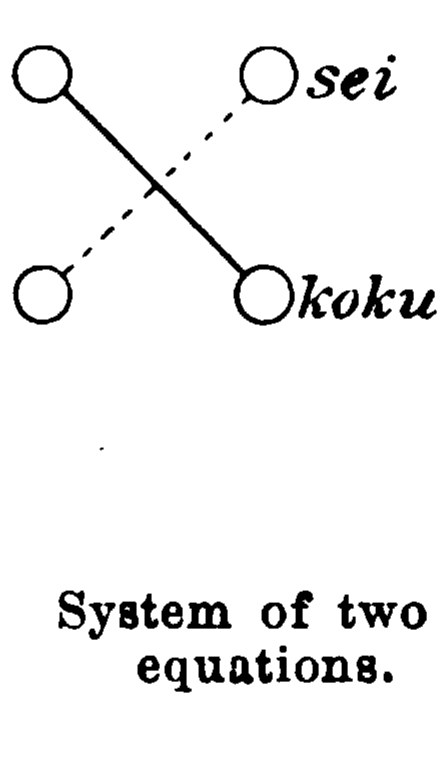
\includegraphics[width=\linewidth]{pdf211-shajo-two-equations.png}
\end{minipage}\hfill
\begin{minipage}[t]{.62\linewidth}
\centering
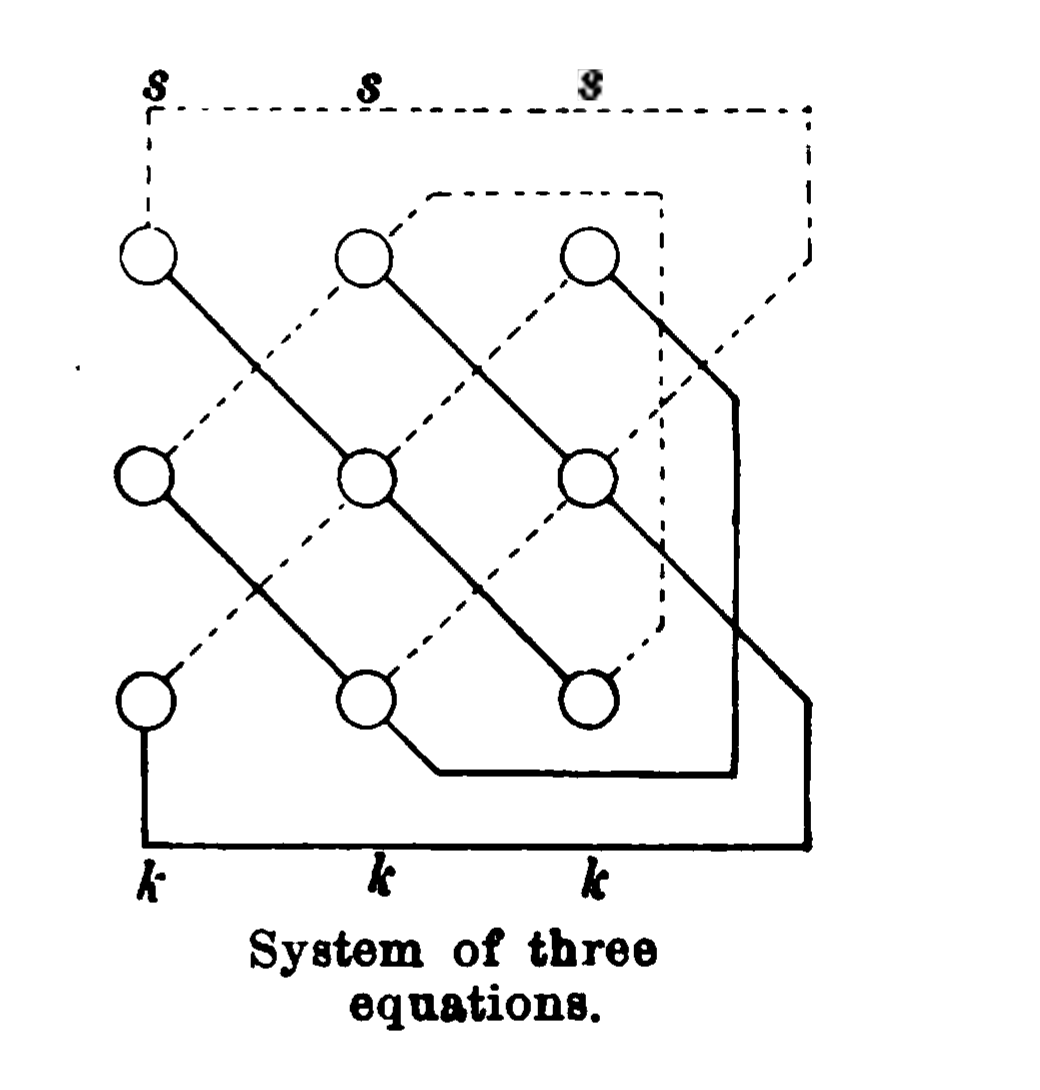
\includegraphics[width=\linewidth]{pdf211-shajo-three-equations.png}
\end{minipage}
\end{center}

この処理が五個より多い方程式の場合にも拡張できることは明らかである。

この操作は \emph{shajō}、すなわち「交乗」と呼ばれる。

\sourceassetJobAJ[width=.91\linewidth]{pdf211-shajo-diagrams-bottom.png}

14. もちろん図に示されていない項がなお存在するが、実際にはそれらもすべて取らなければならない。これを行うため、
\scanfooter

\scanpage{0212}{第24章、印刷頁198}
Seki は方程式を取る順序の交換を用いる。この操作は \emph{kōshiki} と呼ばれる。彼の説明は確かにきわめて簡略であるが、同時に手続の性質を示すには十分である。彼は次のように述べる。

「\emph{kōshiki、すなわち方程式の交換。} 三つの置換方程式の場合から四つの場合を導き、四つの場合から五つの場合を導き、以下同様とする。二つまたは三つの置換方程式については \emph{kōshiki}、すなわち交換は不要である。正順と逆順（\emph{jun} と \emph{gyaku}）はいずれも順次 .1 だけ増し、それによって次の次数を得る。置換方程式の個数が奇数ならすべて正順、偶数なら正順と逆順が交互に来る。」

この説明には次の表が添えられている。\footnote{これらの表は右から左へ読むべきである。文字 $o$ と $r$ は order と reverse を表す（原文では ``stands''）。}

\sourceassetJobAJ[width=.92\linewidth]{pdf212-koshiki-tables.png}

連続する組の形成は、たとえば $2,4,3,1$ という一つの順序を取り、その各数に 1 を加え、その組の右に 1 を配置して $3,5,4,2,1$ を得、これを五方程式の場合の中央の組とすることによって行う。

交換の正順と逆順は図から分かる。上図では前者を右側へ、後者を左側へ行う。
\scanfooter

\scanpage{0213}{第24章結末、印刷頁199}
この操作を \emph{shajō} の操作とともに行えば、行列式の展開に必要なすべての項を得ることができる（原文では ``obtain·all''）。Seki の書では、\emph{kōshiki} は \emph{shajō} より前に記述されている。

15. 各項の \emph{sei} と \emph{koku} が決定されたなら、それぞれの符号を考えなければならない。たとえば与えられた系が
\[
\begin{vmatrix}
I&F&C\\
H&E&B\\
G&D&A
\end{vmatrix}
\qquad\text{または}\qquad
\begin{vmatrix}
-1&4&-3\\
4&-5&1\\
-3&1&2
\end{vmatrix}
\]
であれば、次を得る。
\[
\begin{array}{lll}
\emph{sei}&CEG=-45&\text{差し引く,}\\
\emph{sei}&IBD=-1&\text{”}\\
\emph{sei}&FHA=+32&\text{加える,}\\
\emph{koku}&CHD=-12&\text{”}\\
\emph{koku}&FBG=-12&\text{”}\\
\emph{koku}&IEA=+10&\text{差し引く.}
\end{array}
\]

これらの量のうち、\emph{sei} と記されたものは正なら加え、負なら引く。\emph{koku} と記されたものは正なら引き、負なら加える。

このようにして所望の消去が行われ、消去された量を含まない方程式に至り、出発した問題を解くために役立つ。

以上から、Seki が行列式の観念を有していたことは非常に明らかである。しかも彼は、不明瞭ながら、自分が考えた次数より高い行列式の場合にも理論を適用できることを示している。しかしこの理論は、その説明者の時代以後、旧日本数学派が栄えた全期間を通じて発展しなかったようである。ある量を含む二方程式間でその量を消去するためにこれほど巧妙に用いられた行列式が、線形連立方程式その他の種類の問題の解法には用いられなかったのは、むしろ奇妙である。
\scanfooter

\scanpage{0214}{第25章冒頭、印刷頁200}
\begin{center}
第25章。\\[1mm]
日本の数学者が用いた $\pi$ の値。
\end{center}
\phantomsection\addcontentsline{toc}{subsection}{第25章　日本の数学者が用いた $\pi$ の値}

およそ十世紀ごろから Ashikaga Shogunate の全治世（一四--一六世紀）を通じて、日本人が古く用いた $\pi$ の値は $3\cdot16$ であった。\footnote{T. Endō, \emph{A short account on the progress about the values of $\pi$ in Japan}（日本語）, \emph{Rigakkai}, vol. 3, no. 3, p. 19.} 同じ $\pi$ の値は、一七〇九年の \emph{Kwatsuyō Sampō}\footnote{Seki の著作の遺稿刊行物。} にも日本の旧値として言及される。

一六二七年の Yoshida の \emph{Jinkōki} は、主として一五九三年の Chinese Ch'êng Tai-wei の著作に基づく論書であったが、そこに与えられた $\pi$ の値は採らなかった。反対に彼は $\pi=3\cdot16$ を用いた。Imamura は一六三九年の \emph{Jugai-roku} で $\pi=3\cdot162$ を与え、門人 Andō Yūyeki は一六六〇年刊の同書注釈において、これを $\pi^2=10$ から得たものとした。Imamura の $\pi$ の値には Yamada (1658), Shibamura (1657), Isomura (1660) その他が従った。

一六六〇年以前、日本人は三十二辺を超える内接多角形を用いて円積を試みなかったので、その値が当然きわめて不正確なままであった。\footnote{前掲 Endō 論文、p. 20.} しかし、ほどなくより正確な結果へ至る試みが現れた。Muramatsu Mosei は一六六三年に \emph{Sansō} を著し、そこで円の測定を公表した。彼は内接 $2^{15}=32768$ 角形の周長から
\[
\pi=3\cdot14159\ 26487\ 77698\ 86924\ 8
\]
を得た。これは八桁まで正しいが、著者はどこまで正しいかを知らなかったので、Tsu Ch'ung-chih の値 $\pi=22/7=3\cdot142657\ldots$ と比較し、$\pi=3\cdot14$ を取らざるを得なかった。Nozawa Teichō は一六六四年の \emph{Dōkai-shō} で同じ値を与えた。Satō Seikō は一六六六年の \emph{Kongenki} で $\pi=3\cdot142$ を与えた。Sumida Kōwun もこの値を用いた。\footnote{Endō の論文、p. 19.} Imamura は晩年に $\pi=3\cdot14$ および $\pi=3\cdot1416$ を用いた。\footnote{同所。} Isomura は著作第二版 (1684) で $\pi$ の値を改め、$3\cdot1416$ を与えた。一六九六年、Ikeda Shōi は \emph{Gyokuyen Kyoku-seki} で $\pi=3\cdot141662$ または $\pi=3\cdot142$ を与えた。一七〇四年の \emph{Sampō Zusetsu} で Itō Yūkō は $\pi=3\cdot1416$ を与えた。この著作は
\scanfooter

\scanpage{0215}{第25章、印刷頁201}
数年後に刊行されたようである。$\pi=3\cdot162=\sqrt{10}$ という値は、一七一八年の \emph{Sankan-ki} で Kambara Ichigaku のような後代の著者にも用いられた。$\sqrt{10}$ に相当する $\pi$ の値は、今日なお日本の一部で大工や木材業者によって用いられている。

Tsu Ch'ung-chih の二つの分数値 $\pi=\frac{22}{7}$ および $\pi=\frac{355}{113}$ は、日本で Seki Kōwa によって再び得られた。前者は Chinese treatises から学ばれたが、後者は彼が新たに計算したらしい。これは一六八三年の \emph{Kenki Sampō} で門人 Takebe Kenkō により初めて公表された。この値が Seki によることは、Takebe 自身が一七二二年の \emph{Fukyū Tetsujutsu} で述べている。同じ値は、一七〇九年の Ōtaka の \emph{Kwatsuyō Sampō} にも与えられた。

日本で用いられた $\pi$ のすべての値を説明することはできないので、最も重要な結果だけを掲げることに限らざるを得ない。

一七〇九年の \emph{Kwatsuyō Sampō} 第四巻では、正方形から $2^{17}$ 角形までの内接多角形を用いた数値計算により円測が行われる。$2^{15}$, $2^{16}$, $2^{17}$ 角形の周長は
\[
\begin{aligned}
\text{(a)}\quad 2^{15}\text{角形}&=3\cdot14159\ 26487\ 76985\ 6708,\\
\text{(b)}\quad 2^{16}\text{角形}&=3\cdot14159\ 26523\ 86591\ 3571,\\
\text{(c)}\quad 2^{17}\text{角形}&=3\cdot14159\ 26532\ 88992\ 7759
\end{aligned}
\]
と求められ、これから次の補正を行う。
\[
\pi=\frac{(b-a)(c-b)}{(b-a)-(c-b)}+b=3\cdot14159\ 26535\ 9.
\]

この $\pi$ の値から次の分数が導かれる。
\[
\frac31,\frac72,\frac{10}3,\frac{13}4,\frac{16}5,\frac{19}6,\frac{22}7,\frac{25}8,
\frac{29}9,\frac{32}{10},\frac{35}{11},\frac{38}{12},\frac{41}{13},\frac{44}{14},\frac{47}{15},\frac{51}{16},
\]
\[
\frac{54}{17},\frac{57}{18},\ldots,\frac{355}{113}.
\]

無名写本 \emph{Taisei Sankyō}\footnote{これは時に Seki に、時に門人 Takebe に帰される。} では、上記の補正過程を反復適用する。正方形から内接 512 角形までの周長から、次の値に達する。
\[
\pi=3\cdot14159\ 26535\ 89793\ 23846\ 2643,
\]
\scanfooter

\scanpage{0216}{第25章、印刷頁202}
ここで初めの二十五桁は正しく与えられている。さらにこの数値から出発して、公式
\[
\frac{\pi}{1}=3+\frac{R_1}{1}=3+\frac{1}{\dfrac{1}{R_1}}=3+\frac{1}{Q_1+\dfrac{R_2}{R_1}}=\cdots
\]
により、$\pi$ の分数値を次のように求められる。
\[
\frac31,\frac{22}7,\frac{333}{106},\frac{355}{113},\frac{103993}{33102},\frac{104348}{33215},\frac{208341}{66317},\frac{312689}{99532},\frac{837719}{265381},
\]
\[
\frac{11\ 46408}{3\ 64913},\qquad \frac{42\ 72943}{13\ 60120},\qquad\text{等。}
\]

Takebe Kenkō は一七二二年の \emph{Fukyū Tetsujutsu} で \emph{Taisei Sankyō} と同じ円積法を用い、内接 1024 角形から
\[
\pi=3\cdot14159\ 26535\ 89793\ 23846\ 26433\ 83279\ 50288\ 41971\ 2
\]
を得た。このうち初めの四十一桁は正しく、末尾の数字は含めない。Matsunaga Ryōhitsu は一七三九年の写本 \emph{Hōyen Sankyō} で
\[
\begin{aligned}
\pi={}&3\cdot14159\ 26535\ 89793\ 23846\ 26433\ 83279\\
&50288\ 41971\ 69399\ 3751
\end{aligned}
\]
を与え、五十桁がすべて正しい。これは級数
\[
\frac{\pi}{3}=1+\frac{1^2}{4\cdot6}+\frac{1^2\cdot3^2}{4\cdot6\cdot8\cdot10}+\frac{1^2\cdot3^2\cdot5^2}{4\cdot6\cdot8\cdot10\cdot12\cdot14}+\cdots
\]
から計算された。

同じ $\pi$ の値は Arima が一七六九年の \emph{Shūki Sampō} で公表し、そこには次の二分数も見られる。
\[
\pi=\frac{54\ 19351}{17\ 25033},\qquad \pi=\frac{42822\ 45933\ 49304}{13630\ 81215\ 70117},
\]
これらは $\pi$ の初めの十三桁および三十桁を正しく与える。

Kurushima Yoshita（一七五七年没）は、\emph{Kyūshi Ikō}、すなわち \emph{Kurushima's Posthumous Writings} で $\pi^2$ の分数値を
\[
\frac{227}{23},\qquad \frac{10748}{1089},\qquad \frac{10975}{1112},\qquad\text{および}\qquad \frac{98548}{9885}
\]
と与えた。

Takebe および Matsunaga とほぼ同時代に、別の数学者 Takuma Genzayemon がいた。彼は $2^{42}$ 辺の内接および外接多角形を用いた数値計算で円積を試み、その周長は次のように求められた。
\scanfooter

\scanpage{0217}{第25章結末および第26章冒頭、印刷頁203}
\[
3\cdot14159\ 26535\ 89793\ 23816\ 26433\ 6658,
\]
\[
3\cdot14159\ 26535\ 89793\ 23846\ 26433\ 67,
\]
この二つの平均を取り、$\pi$ の二十六桁まで正しい値が次のように確立された。\footnote{Endō の論文、No. 4, pp. 21--22.}
\[
\pi=3\cdot14159\ 26535\ 89793\ 23846\ 26433.
\]

\begin{center}
第26章。\\[1mm]
日本の数学者による球体積の研究。
\end{center}
\phantomsection\addcontentsline{toc}{subsection}{第26章　日本の数学者による球体積の研究}

1. 十七世紀の日本数学者は球の体積に種々の値を与えた。その最初期の例は、一六三九年の Imamura の \emph{Jugairoku} と Yoshida の \emph{Jinkōki} 新版である。単位直径の球体積について Imamura は $0\cdot51$ を与え、Yoshida は $0\cdot5625$ を与えた。\footnote{この値は一六二七年の \emph{Jinkōki} にはない。後の一版に、解答を求める問題とともに収められていたが、その版は失われた。} 後者が大きすぎることは容易に分かる。Yamada は一六五六年に \emph{Kaisanki} を刊行し、これを訂正して $0\cdot5$ より小さいとした。後続著者の値は次のとおりである。

\begin{center}
\begin{tabular}{l|l|c|c}
\text{著者}&\text{書名}&\text{年}&\text{値}\\ \hline
Shibamura&Kakuchi Sansho&1657&$0\cdot525$\\
Isomura&Ketsugi-shō&1660&$0\cdot510$\\
Muramatsu&Sansō&1663&$0\cdot524$\\
Nozawa&Dōkaishō&1664&$0\cdot523$\\
Satō&Kongen-ki&1666&$0\cdot519$\\
Okuda&Shimpen Sansūki&1681&$0\cdot555$\\
Isomura&(第二版)&1684&$0\cdot5236$\\
Miyagi&Wakan Sampō&1695&$0\cdot51$
\end{tabular}
\end{center}

これらの著者の時代、球体積の計算法は、平行平面で球を等しい厚さの薄片に分け、その一薄片の体積を、その両底面上に同じ高さで立てた二円柱の体積の平均とし、全薄片について和を取るものであった。最終値の相違は、球を分ける個数と、用いた円の面積係数の値の相違から生じた。
\scanfooter

\scanpage{0218}{第26章、印刷頁204}
例として、一六八四年版 \emph{Ketsugishō} で Isomura が述べることを再録する。

「直径一尺の球を一〇〇〇〇片に切れば、各片の厚さは $0\cdot0001$ 尺であり、非常に薄い紙ほどになる。このように各片の体積を求め、一〇〇〇〇個の結果を合計すると、$523\cdot6$ measure を得る。\footnote{ここで単位は一尺の十分の一の立方である。} そのほか、確かに小さな通約不能部分があるが、それらは捨てる。」

2. Seki Kōwa の遺著である Ōtaka の \emph{Kwatsuyō Sampō} には、球体積の評価に当てられた一章がある。先行者と同様の考察に従い、Seki は球を五〇、百、二百片に切り、それらの和を
\[
a=0\cdot6664,\qquad b=0\cdot6666,\qquad c=0\cdot66665
\]
と求める。ここでは因子 $\frac14\pi$ を省いている。円周計算で用いた補正過程（p. 201 参照）をこれら三量に施すと、$0\cdot666\frac23$ を得る。これに $\frac\pi4=\frac14\times\frac{355}{113}$ を掛け、球体積の最終結果
\[
0\cdot523\frac{203}{339}=\frac{355}{6\times113}=d^3\times\frac\pi6
\]
を得る。

3. Matsunaga は \emph{Sampō Shūsei} において、この球体積計算法を不満足とし、よりよい解析的処理を与えようとした。

球を等しい厚さの $n$ 薄片に分けるとする。各切断面を底とする球冠の矢高を、大きさの順に $s_1,s_2,s_3,\ldots$ とする。$d$ を球の直径とすれば、これらは明らかに
\[
\frac dn,\quad \frac{2d}{n},\quad \frac{3d}{n},\quad\ldots
\]
である。断面円の直径を $c_1,c_2,\ldots$ とすれば、
\[
c_r^2=4(d-s_r)s_r=4rds_1-4r^2s_1^2
\]
と表される。これに $\frac14\pi$ と共通厚さ $s_1$ を掛け、総和を取ると、
\[
4\times\frac{\pi}{4}\times ds_1^2(1+2+3+\cdots+n)-4\times\frac{\pi}{4}\times s_1^3(1^2+2^2+3^2+\cdots+n^2)
\]
\[
=\pi ds_1^2\left(\frac{n^2}{2}+\frac n2\right)-\pi s_1^3\left(\frac{2n^3}{6}+\frac{3n^2}{6}+\frac n6\right)=\frac{\pi}{6}d^3-\frac{\pi}{6}d^3\frac1{n^2}
\]
を得る。
\scanfooter

\scanpage{0219}{第26章、印刷頁205}
ここで分割数 $n$ は望むだけ大きく考えられるので、その冪の逆数は望むだけ小さくできる。したがって最後には後者を捨て、球体積として $\frac16\pi d^3$ を得る。

同じ手続は、同じ著者の \emph{Ritsuyen Ritsu}（球の解析）、門人 Yamaji の \emph{Gyokuseki Shinjutsu}（球体積を求める精密法）、第二題 \emph{Yenri Kenkon Sho} を持ち、時に Seki の方法を含むとされる無名写本 \emph{Kigenkai} にも従われる。このため、今述べた解析を Seki に帰する学者もいる。\footnote{T. Endō, Proc. of Tokyo M. P. S., vol. 7, pp. 123--126.}

4. 同じ解析法は球欠の場合にも同様に適用でき、上記写本に記録されている。底面に平行な断面によって球欠を $n$ 部分に分け、矢高 $s$ を各 $\frac1n s$ の $n$ 部分に切る。矢高の端から数えた断面円の直径を $c_1,c_2,\ldots$ とすれば、
\[
c_r^2=4\left(d-r\times\frac{s}{n}\right)r\frac{s}{n}=\frac{4ds}{n}\times r-\frac{4s^2}{n^2}\times r^2,
\]
\[
\therefore\sum_{r=1}^{r=n}c_r^2=\frac{4ds}{n}\sum_{r=1}^{r=n}r-\frac{4s^2}{n^2}\sum_{r=1}^{r=n}r^2
=\frac{4ds}{n}\times\frac{n+n^2}{2}-\frac{4s^2}{n^2}\times\frac{n+3n^2+2n^3}{6},
\]
\[
\therefore\frac{\pi}{4}\times\frac{s}{n}\times\sum_{r=1}^{r=n}c_r^2
=\frac{\pi}{6}\times s^2\times\left\{\frac{3d}{n}+3d-\frac{s}{n^2}-\frac{3s}{n}-2s\right\},
\]
したがって極限 $n=\infty$ に移れば、球欠体積 $=\frac16\pi s^2(3d-2s)$ を得る。

上記の球および球欠の体積を求める方法は、日本数学の \emph{yenri} 法における無限小的考察の進歩に寄与したかもしれない。先行者のように弧または円周を等分する代わりに、直径または弦を等分することを導入した Ajima の円理改良は、確かに球の処理を模倣して行われた。

5. Wada Nei (1787--1840) は体積要素
\[
\left\{d^2-\left(r\times\frac dn\right)^2\right\}\cdot\frac dn\cdot\frac\pi4=d^3\frac\pi4\left(\frac1n-\frac{r^2}{n^3}\right)
\]
を取った。
\scanfooter

\scanpage{0220}{第26章結末および第27章冒頭、印刷頁206}
そして表による「畳み」、すなわち積分の操作をこれに施し、直ちに
\[
d^3\times\frac\pi4\left(1-\frac13\right)=\frac16d^3\pi
\]
を得た。

Wada の先行者は常に、要素を合計し、その和の極限値を求める全段階を経た。しかし「畳み表」を用いることで、彼はこれらすべてを一操作で行うことができ、相当量の労力が省かれた。

\begin{center}
第27章。\\[1mm]
球面積を求めることに関する日本数学者の研究。
\end{center}
\phantomsection\addcontentsline{toc}{subsection}{第27章　球面積を求めることに関する日本数学者の研究}

1. Imamura Chishō は一六三九年の \emph{Jugai-roku} で、球面積をその円周の平方の四分の一とした。同じものは Isomura が一六六〇年の \emph{Ketsugi-sho} で採用した。当時の日本数学者の間で一般に用いられていたらしく、Isomura は一六八四年刊の第二版でこれを旧法と呼ぶ。この版で彼は公式の不正確さに気づいたが、彼によれば Mōri、Yoshida、Imamura、Takahara、Hiraga、Shimada、Sumida その他の数学者は球面積の正しい公式を見いだせなかった。Isomura は次のように測定を試みた。

直径 10 と $10\cdot0002$ の球体積は、それぞれ $523\cdot6$ と $523\cdot63141\ 66283\ 24188\ 8$ であり、その差は $0\cdot03141\ 66283\ 24188\ 8$ である。これを二表面間の殻の厚さ $0\cdot0001$ で割ると、厚さ $0\cdot0001$ の殻の表面として $314\cdot16628\ 32418\ 88$ を得る。また直径 $9\cdot9998$ の球体積は $523\cdot56858\ 64283\ 15811\ 2$ であり、直径 10 の球体積との差を厚さ $0\cdot0001$ で割れば、この場合の殻の表面は $314\cdot15371\ 68418\ 88$ となる。球面積はこれら二面積の平均、すなわち
\[
314\cdot16000\ 00418\ 88
\]
で与えられる。しかし球体積が $523\cdot6$ であるから、
\[
523\cdot6\times6=3141\cdot6
\]
であり、したがって
\[
(\text{表面積})=\frac{(\text{体積})\times6}{(\text{直径})},\qquad\text{または}= (\text{直径})^2\times\pi
\]
となる。
\scanfooter

\scanpage{0221}{第27章、印刷頁207}
2. Isomura と同じ球面積評価法は、Takebe Kenkō も一七二二年の \emph{Fukyū Tetsujutsu} で採用した。しかし Takebe は二値の平均を取らず、別の仕方で進めた。直径 $10\cdot01$, $10\cdot0001$, $10\cdot00000\ 01$ の球から直径 10 の球を除いて殻を作り、それぞれの厚さで割った商を
\[
314\cdot47352\ 9344,\qquad 314\cdot16240\ 6984,\qquad 314\cdot15929\ 677
\]
と求め、Ōtaka の \emph{Kwatsuyō Sampō} に与えられた補正過程を適用する。これらを $a,b,c$ とすれば、球面積の補正値は
\[
(\text{表面積})=b-\frac{(a-b)(b-c)}{(a-b)-(b-c)}=314\cdot15926\ 5359
\]
となる。

この値が数字の位置を除いて $\pi$ と同じであることから、Takebe は直ちに球面積を $(\text{直径})^2\pi$ と書く。

3. Takebe の \emph{Fukyū Tetsujutsu} によれば、Seki は同じ目的に異なる考察法を用いた。Seki は球の中心を円錐の頂点とし、半径を高さ、球体積を円錐の体積とした。したがって
\[
\frac13(\text{表面積})(\text{半径})=(\text{円錐体積})=(\text{球体積}),
\]
\[
\therefore\quad (\text{球面積})=\frac{3\times(\text{球体積})}{(\text{半径})}
\]
を得、これは Isomura の公式と一致する。

この攻め方を用いた Seki は、Isomura と Takebe が確立した手続を取るに足りないものとして軽蔑した。しかし Takebe は、自分は Seki に同意しないと強調する。

4. 前に述べた無名写本 \emph{Kigen-kai} には、回転軸 $a=1$ 尺、他軸 $b=0\cdot6$ 尺の回転楕円体の表面を評価する一章がある。この楕円体の体積を、$a,b$ の値が
\[
\begin{array}{c|c|c|c|c}
a&1\cdot001&1\cdot0001&1\cdot00001&1\cdot000001\\
b&0\cdot601&0\cdot6001&0\cdot60001&6\cdot000001
\end{array}
\]
である楕円体の体積から引き、その差を殻の各厚さ $0\cdot0005$, $0\cdot00005$, $0\cdot000005$, $0\cdot00000\ 05$ で割ると、省かれた因子 $\frac16\pi$ を除き、結果は次のようになる。
\scanfooter

\scanpage{0222}{第27章、印刷頁208}
\[
\begin{aligned}
A&=3\cdot12440\ 2,&\qquad C&=3\cdot12004\ 40002,\\
B&=3\cdot12044\ 002,&D&=3\cdot12000\ 44000\ 02.
\end{aligned}
\]
これらの値の逐次差は
\[
F=0\cdot00396\ 198,\qquad H=0\cdot00039\ 60198,
\]
\[
K=0\cdot00003\ 96001\ 98;
\]
\[
\therefore\quad \frac HF=\frac{6667}{66700},\qquad \frac KH=\frac{66667}{6\ 66700},\qquad\text{または}\qquad \frac{H\mid F}{K\mid H}=\frac{444\ 48889}{444\ 66889}.
\]
ここでは、この最後の量が 1 にならないため、そこから結論を導けないと論じる。そのため著者は別の方法を取る。

二楕円体 $(a,b)$ と $(a'=a+2h,b'=b+2h)$ の体積差を $h$ で割った商は、因子 $\frac16\pi$ を除けば、
\[
\frac{(a+2h)(b+2h)^2-ab^2}{h}=4ab+2b^2+h(4a+8b+8h)
\]
である。

上記の $a,b$ の値を取り、
\[
2h=0\cdot001,\quad 0\cdot0001,\quad 0\cdot00001,\quad 0\cdot00000\ 1
\]
と置くと、上式で $h$ を掛けた量は
\[
\begin{aligned}
A'&=0\cdot00440\ 2,&\qquad C'&=0\cdot00004\ 40002,\\
B'&=0\cdot00044\ 002,&D'&=0\cdot00000\ 44000\ 02
\end{aligned}
\]
となる。

これらをそれぞれ $A,B,C,D$ と名づけた量から引けば、余りは等しくなる。実際の場合には厚さは存在しないと考えれば、$h$ を掛けた項を捨てられる。したがって、省いた因子 $\frac16\pi$ を戻すと、表面は
\[
\frac\pi6(4ab+2b^2)=(b^2+2ab)\frac\pi3
\]
で与えられる。

この結果は正しくないが、用いられた手続の考え方は、歴史上いくらか興味があるかもしれない。

5. Tani Shōmo の一八二五年または一八二七年の写本 \emph{Tetsujutsu Shin-i} では、回転楕円体の表面を求める問題が異なる方法で扱われる。その結果は
\[
(\text{表面積})=ab\pi\left(1-\frac m6-\frac{m^2}{40}-\frac{m^3}{112}-\frac{m^4}{1152}-\cdots\right),
\]
ここで $m=1-\frac{b^2}{a^2}$ とする。$t=\frac{ab\pi}{\sqrt m}$ と書けば、これは次のように書ける。
\scanfooter

\scanpage{0223}{第27章、印刷頁209}
\[
\frac{(\text{表面積})}{t}=\sqrt m-\frac{\sqrt{m^3}}6-\frac{\sqrt{m^5}}{40}-\frac{\sqrt{m^7}}{112}-\frac{\sqrt{m^9}}{1152}-\cdots,
\]
これは、距離 $\sqrt m$ を隔てた二本の等長平行弦の間に含まれる、直径 1 の円の一部分の面積を表す公式であることが分かる。しかし後者の面積は
\[
\frac14\pi-2\times(\text{弦 }c=\sqrt{1-m^2}=a/b\text{ を持つ弓形の面積})
\]
であるから、Tani は回転楕円体の表面を
\[
(\text{表面積})=\frac1{\sqrt m}\left\{\frac\pi6\times\pi\times ab-2\times ab\pi\,(\text{弓形面積})\right\}
\]
で表す。

Tani は、この公式が Ikeda Teiichi の門人 Kinoshita Teichi によっても得られ、一八二三年に Yedo の Shintō temple の前へ掲額されたと述べる。その結果は Shiraishi Chōchū が一八二六年の \emph{Shamei Sampu} で公表した。

Tani はまた、回転軸に垂直な二平面で切り取られた同じ立体の一部分の面積公式を得た。

Shiraishi による楕円体表面の測定は第三十八章で考察する。

6. さて本題に戻ると、二球の体積差から球面積を求める方法は、Tani と同時代の Wada Nei によって再び用いられた。Isomura と Takebe と同じ追求に属するとはいえ、Wada の考察は解析的に行われた。直径 $d$ と $d+h$ の二球を取れば、その体積差は
\[
(d+h)^3\frac\pi6-d^3\frac\pi6=\frac\pi6(3d^2h+3dh^2+h^3)
\]
である。

この殻を平面図形に展開したと考えれば、その厚さは $\frac12h$ であるから、表面は $\frac13\pi(3d^2+3dh+h^2)$ となる。しかし $h$ は望むだけ小さく考えられるので、極限では $\frac13\pi\times3d^2=d^2\pi$ に帰着し、これは球面積を表す。Wada の解析は、回転楕円体について \emph{Kigen-kai} に与えられたものと一致する。

7. Hasegawa Kan の一八三〇年刊 \emph{Sampō Shinsho} でも、同じ球面積測定法が公表された。ここでは次の式が用いられる。
\[
(\text{表面積})\times h=d^3\frac\pi6-(d-2h)^3\frac\pi6.
\]
\scanfooter


\scanpage{0224}{第28章冒頭、印刷頁210}
\begin{center}
第28章。\\[1mm]
1709 年の \emph{KWATSUYŌ SAMPŌ} における\\
円弧の平方の公式。
\end{center}
\phantomsection\addcontentsline{toc}{subsection}{第28章　1709 年の KWATSUYŌ SAMPŌ における 円弧の平方の公式}

Seki Kōwa の著述から Ōtaka Yūshō が一七〇九年に編纂し、一七一二年に刊行した \emph{Kwatsuyō Sampō} 第四巻には、円弧の平方の公式がある。それは次のものである。
\[
\begin{aligned}
12\,76900(d-s)^5(\mathrm{arc})^2={}&51\,07600d^6s-238\,35413d^5s^2\\
&+434\,70240d^4s^3-379\,97429d^3s^4+150\,47062d^2s^5\\
&-15\,01025ds^6-2\,81290s^7,
\end{aligned}
\]
ここで $d$ は直径、$s$ は矢高である。

この公式の構成について同書には若干述べられているが、それはほとんど理解できない。しかし、無名の \emph{Kigenkai}、Matsunaga の \emph{Sampō Shūsei}、一七七四年の日付を持つ Ōba Keimei の \emph{Kwatsuyō Kojutsu no Kai}、すなわち「\emph{Kwatsuyō Sampō} における円弧公式についての注」など、諸写本に与えられた説明を調べると、その手順は明らかになる（原文では ``precedure''）。ここでは解析の簡潔な記述を与えることにする。

まず第一に、直径が一尺で、矢高が $s_1=0\dd1$, $s_2=0\dd2$, $s_3=0\dd3$, $s_4=0\dd4$, $s_5=0\dd45$, $s_0=0\dd5$ である円の弧を数値計算によって求める。この計算は、二辺の正多角形線を内接させ、辺数を逐次倍加して $2^{15}=32768$ 辺の多角形線に達するまで行う。すでに述べた全円周の場合と同じ整直法を適用し、分数値の $\pi$ との対応を保つため、結果に $\pi=\frac{355}{113}$ を掛け、$\pi=3\dd14159\,26535\,9$ で割ると、これらの弧は
\[
\begin{aligned}
x_1&=0\dd64350\,11087\,93284\,3868,\\
x_2&=0\dd92729\,5218,\\
x_3&=1\dd15927\,94807\,3,\\
x_4&=1\dd36943\,84060\,1,\\
x_5&=1\dd47062\,89056\,3.
\end{aligned}
\]
となる。次に $r=1,2,3,4,5$ に対して、量 $\alpha_r$ を次のように作る。
\[
\alpha_r=s_r^2k+4(d-s_r)s_r-x_r^2,
\]
\scanfooter

\scanpage{0225}{第28章、印刷頁211}
ここで $k$ は
\[
k=\frac{355^2-4\times113^2}{113^2}=5\dd86960\,60772\,18.
\]
を表す。

ここに $s_r=\frac12d$ または $s_r=s_0$ と置けば、$\alpha_r$ が消えることは明らかである。これらの量 $\alpha$ は「弧平方の差」と呼ばれる。これらの差の数値は
\[
\begin{aligned}
\alpha_1&=0\dd00460\,23178\,51,\\
\alpha_2&=0\dd01490\,76696\,87,\\
\alpha_3&=0\dd02433\,54023\,45,\\
\alpha_4&=0\dd02377\,51122\,95,\\
\alpha_5&=0\dd01584\,54867\,58.
\end{aligned}
\]
である。さらに「三次冪の差」を次のように作る。
\[
\beta_r=\frac{m_1s_r^2(d-2s_r)}{d-s_r}-\alpha_r,
\]
ここで
\[
m_1=\frac{\alpha_1(d-s_1)}{(d-2s_1)s_1^2}=0\dd51776\,07582\,2,
\]
そして次の量を作る。
\[
\begin{aligned}
m_2&=\frac{\beta_2(d-s_2)^2}{(d-2s_2)s_2^2(s_2-s_1)}=0\dd16670\,74826\,5,\\[1mm]
\gamma_r&=\frac{m_2(s_r-s_1)s_r^2(d-2s_r)}{(d-s_r)^2}-\beta_r,\\[1mm]
m_3&=\frac{\gamma_3(d-s_3)^3}{(d-2s_3)s_3^2(s_3-s_1)(s_3-s_2)}=0\dd07492\,90858\,3,\\[1mm]
\delta_r&=\frac{m_3(s_r-s_2)(s_r-s_1)s_r^2(d-2s_r)}{(d-s_r)^3}-\gamma_r,\\[1mm]
m_4&=\frac{\delta_4(d-s_4)^4}{(d-2s_4)s_4^2(s_4-s_1)(s_4-s_2)(s_4-s_3)}=0\dd04002\,63239\,5,\\[1mm]
\varepsilon_4&=\frac{m_4(s_r-s_3)(s_r-s_2)(s_r-s_1)s_r^2(d-2s_r)}{(d-s_r)^4}-\delta_r,\\[1mm]
m_5&=\frac{\varepsilon_5(d-s_5)^5}{(d-2s_5)s_5^2(s_5-s_1)\cdots(s_5-s_4)}=0\dd02523\,31671\,5,\\[1mm]
\zeta_r&=\frac{m_5(s_r-s_4)\cdots(s_r-s_1)s_r^2(d-2s_r)}{(d-s_r)^4}-\varepsilon_r.
\end{aligned}
\]

ここで $\beta_1$；$\gamma_1$, $\gamma_2$；$\delta_1$, $\delta_2$, $\delta_3$；$\varepsilon_1$, $\varepsilon_2$, $\varepsilon_3$, $\varepsilon_4$；$\zeta_1$, $\zeta_2$, $\zeta_3$, $\zeta_4$, $\zeta_5$；はいずれも $=0$ であることが容易に分かる。$\alpha_r=A$ と書き、$\beta_r$, $\gamma_r$, $\delta_r$, $\varepsilon_r$, $\zeta_r$ の式の第一項をそれぞれ $B$, $C$, $D$, $E$, $F$ と表すと、
\[
\zeta_r=F-E+D-C+B-A.
\]
であることは明らかである。
\scanfooter

\scanpage{0226}{第28章結末、印刷頁212}
しかし $r=1,2,3,4,5$ に対して $\zeta_r=0$ であるから、
\[
A-B+C-D+E-F=0,
\]
を得る。これは $s_r$ が $s_1$, $s_2$, $s_3$, $s_4$, $s_5$ に等しい各値について成り立つ。また $s_r=s_0=\frac12d$ についても、同じ $s_r$ の値では明らかに $\beta$, $\gamma$, $\delta$, $\varepsilon$ がすべて消えるので、成り立つ。したがって、上の関係において $x_r$ を $x$ で、$s_r$ を $s$ で置き換えると、$s=s_0,s_1,s_2,\ldots,s_5$ について存在するこの関係は、実際上、矢高 $s$ の他の任意の値についても存在すると考えることができる。ゆえに、与えられた矢高に対応する任意の弧長を定めるためにこれを用いることができる。

上で表した \emph{Kwatsuyō Sampō} の公式は、今述べた関係を変形し簡約して得られる結果である。

$\alpha$, $\beta$, $\gamma$ などの実際の値は、それらが徐々に小さくなることを示すため計算されている。$\alpha$ の値はすでに与えた。$\beta$, $\gamma$, \ldots の値は
\[
\begin{array}{r@{\;}c@{\;}l|r@{\;}c@{\;}l}
\beta_2&=&0\dd00625\,15305\,99&\gamma_4&=&0\dd00606\,73806\,08\\
\beta_3&=&0\dd02292\,29379\,23&\gamma_5&=&0\dd00688\,39200\,96\\
\beta_4&=&0\dd03838\,79480\,99&\delta_4&=&0\dd00059\,29825\,77\\
\beta_5&=&0\dd03217\,52297\,65&\delta_5&=&0\dd00109\,59431\,02\\
\gamma_3&=&0\dd00157\,28554\,46&\varepsilon_5&=&0\dd00006\,66273\,69
\end{array}
\]
である。

公式を導く推論はこのように非常に明瞭であるが、同時に、何が Seki にこのような方法を思いつかせたのかは、なお非常に疑わしい。この点については、われわれは今後の研究成果を切望する。これと \emph{shōsa} 法との関係もまた明らかにされなければならない。いずれにせよ、この公式の構成は歴史的観点からきわめて興味深いものでなければならない。無限級数で表された公式ほど一般的でないとしても、その歴史的価値は後者に劣るものと決して見なされない。それは解析的考察の成立への鍵であった可能性も少なくない。このすべてがこれまで日本数学史の著述家の注意を免れてきたことは、むしろ驚くべきことである。
\scanfooter

\scanpage{0227}{第29章冒頭、印刷頁213}
\begin{center}
第29章。\\[1mm]
日本の数学者が用いた $\pi$ の若干の級数。
\end{center}
\phantomsection\addcontentsline{toc}{subsection}{第29章　日本の数学者が用いた $\pi$ の若干の級数}

一七世紀および一八世紀の日本の数学者が用いた $\pi$ の値については、すでに述べた。ここでは、一八世紀および一九世紀の学者が $\pi$ とその冪について与えた若干の無限級数を示す。

われわれが出会う最初の例は、一七二八年の Tanzan Shōkei の写本 \emph{Yenri Hakki} に得られている $\pi^2$ の二級数である。そこに記述された解析は Takebe Kenkō に帰せられている。二級数は
\[
\tag{1}\pi^2=8\left(1+\frac16+\frac{1\dd4}{6\dd15}+\frac{1\dd4\dd9}{6\dd15\dd28}+\cdots\right),
\]
\[
\tag{2}\pi^2=4\left(1+\frac26+\frac{2\dd8}{6\dd15}+\frac{2\dd8\dd18}{6\dd15\dd28}+\cdots\right),
\]
であり、Takebe の級数（164頁に掲げた）に、それぞれ $s=\frac12d$ と $s=d$ を置いて得られた。

Matsunaga は一七三九年または一七三八年の \emph{Hōyen Sankyō} に、二級数
\[
\tag{3}\pi^2=9\left(1+\frac{1^2}{3\dd4}+\frac{1^2\dd2^2}{3\dd4\dd5\dd6}+\frac{1^2\dd2^2\dd3^2}{3\dd4\dd5\dd6\dd7\dd8}+\cdots\right),
\]
\[
\tag{4}\pi=3\left(1+\frac{1^2}{4\dd6}+\frac{1^2\dd3^2}{4\dd6\dd8\dd10}+\frac{1^2\dd3^2\dd5^2}{4\dd6\dd8\dd10\dd12\dd14}+\cdots\right).
\]
を与えた。Matsunaga が五十桁まで正しい $\pi$ の値を計算したのは級数 (4) からである。

一八一〇年に書かれ、その後数年の間に印刷された Sakabe の \emph{Tenzan Shinanroku} には、次の級数が見られる。
\[
\tag{5}\pi=4\left(1-\frac15-\frac{1\times4}{5\dd7\dd9}-\frac{1\dd3\times4\dd6}{5\dd7\dd9\dd11\dd13}-\frac{1\dd3\dd5\times4\dd6\dd8}{5\dd7\cdots17}-\cdots\right).
\]

一八三〇年に印刷された Hasegawa Kan の \emph{Sampō Shinsho} では、この級数は、第一項を除いて、次の級数の各二項を結合して得られるものとして示されている。
\[
\tag{6}\frac{\pi}{4}=1-\frac16-\frac1{6\times5}-\frac{1\dd2}{6\times5\dd7}-\frac{1\dd2\dd3}{6\times5\dd7\dd9}-\frac{1\dd2\dd3\dd4}{6\times5\dd7\dd9\dd11}-\cdots.
\]

Hasegawa Kō は、弟子 Uchida Kyūmei の名で刊行された一八四四年の \emph{Kyūseki Tsūkō} に、次の級数を与えた。
\[
\tag{7}\frac{\pi}{4}=1-\frac1{2\dd3}-\frac1{8\dd5}-\frac3{48\dd7}-\frac{15}{384\dd9}-\frac{105}{3840\dd11}-\cdots,
\]
\scanfooter

\scanpage{0228}{第29章、印刷頁214}
すなわち、次の形に書き直される。
\[
\tag{8}\frac{\pi}{4}=1-\frac1{3!}-\frac{1^2\dd3}{5!}-\frac{1^2\dd3^2\dd5}{7!}-\frac{1^2\dd3^2\dd5^2\dd7}{9!}-\cdots.
\]

Kawai Kyūtoku は写本 \emph{Shin Koyen-Jutsu} に、級数
\[
\tag{9}\pi=2\left(1+\frac{1^2}{3!}+\frac{3^2}{5!}+\frac{3^2\dd5^2}{7!}+\frac{3^2\dd5^2\dd7^2}{9!}+\cdots\right),
\]
\[
\tag{10}\frac{\pi}{4}=\frac23+\frac2{2\times3\dd5}+\frac{2\dd3}{2\times3\dd5\dd7}+\frac{2\dd3\dd4}{2\times3\dd5\dd7\dd9}+\frac{2\dd3\dd4\dd5}{2\times3\dd5\dd7\dd9\dd11}+\cdots.
\]
を与えた。この二級数について Kawai は、前者は収束が非常に遅いので不便であると言う。この写本には級数 (8) も見られる。Kawai は Sakabe の弟子であった。

Wada Nei（一七八七--一八四〇）は次の級数を与えたとされる。
\footnote{T. Endō の \emph{Rigakkai}, vol. 3, no. 4, p. 24 所収論文。}
\[
\tag{11}\frac{\pi}{3}=1+\frac1{3\dd2\dd4}+\frac3{5\dd8\dd4^2}+\frac{15}{7\dd48\dd4^3}+\frac{105}{9\dd384\dd4^4}+\cdots,\footnotemark
\]
\footnotetext{異なる形で与えられた (4) と同じ。}
\[
\tag{12}\frac{\pi}{2}=1+\frac1{3\dd2}+\frac3{5\dd8}+\frac{15}{7\dd48}+\frac{105}{9\dd384}+\cdots,
\]
\[
\tag{13}\frac{\pi}{4}=\frac13+\frac1{5\dd2}+\frac3{7\dd8}+\frac{15}{9\dd48}+\frac{105}{11\dd384}+\cdots,
\]
\[
\tag{14}\frac{\pi}{8}=\frac13+\frac1{15\dd2}+\frac3{35\dd8}+\frac{15}{63\dd48}+\frac{105}{99\dd384}+\cdots,
\]
\[
\tag{15}\frac{\pi}{32}=\frac1{15}+\frac1{35\dd2}+\frac3{63\dd8}+\frac{15}{99\dd48}+\frac{105}{143\dd384}+\cdots,
\]
\[
\tag{16}\frac{\pi}{4}=1-\frac13+\frac3{15}-\frac{15}{105}+\frac{105}{945}-\frac{945}{10395}+\cdots,
\]
\[
\tag{17}\frac{\pi}{8}=\frac7{15}+\frac{11\dd1}{105}+\frac{15\dd3}{945}+\frac{19\dd15}{10395}+\frac{23\dd105}{135135}+\cdots,
\]
\[
\tag{18}\frac{\pi}{2\sqrt2}=1+\frac1{3\dd2\dd2}+\frac3{5\dd8\dd2^2}+\frac{15}{7\dd48\dd2^3}+\frac{105}{9\dd384\dd2^4}+\cdots,
\]
\[
\tag{19}\frac{\pi}{8}=\frac12-\frac1{15}-\frac1{63}-\frac1{143}-\frac1{255}-\cdots.
\]

Wada の著述に基づく Koide Shūki の一八四二年の写本 \emph{Yenri Sankyō} には、二級数
\[
\tag{20}\frac{\pi}{4}=1-\frac13+\frac15-\frac17+\frac19-\frac1{11}+\cdots,
\]
\[
\tag{21}\frac{\pi}{4}=1-\frac1{3\dd2}-\frac1{5\dd8}-\frac3{7\dd48}-\frac{15}{9\dd384}-\frac{105}{11\dd3840}-\cdots,
\]
が見られ、そのうち前者は (16) と同じである。
\scanfooter

\scanpage{0229}{第29章、印刷頁215}
\emph{yenri} 計算に必要な若干の表を与える無名写本 \emph{Sampō Yenri Hyō} は、おそらく Wada によるものであり、次の級数を含む。
\[
\tag{22}\frac{\pi}{2\sqrt3}=1-\frac1{3\dd3}+\frac1{5\dd3^2}-\frac1{7\dd3^3}+\frac1{9\dd3^4}-\cdots,
\]
\[
\tag{23}\pi=\frac12\left(1-\frac1{2^2}-\frac3{8^2}-\frac{3\dd15}{48^2}-\frac{15\dd105}{384^2}-\cdots\right),
\]
\[
\tag{24}\pi=2\sqrt3\left(\frac1{3\dd2\dd2}+\frac1{5\dd8\dd2^2}+\frac1{7\dd48\dd2^3}+\frac1{9\dd384\dd2^4}+\cdots\right),
\]
\[
\tag{25}\pi^2=4\left(1+\frac2{2\dd3}+\frac8{3\dd15}+\frac{48}{4\dd105}+\frac{384}{5\dd945}+\cdots\right),
\]
\[
\tag{26}\pi^2=8\left(1+\frac2{2\dd3\dd2}+\frac8{3\dd15\dd2^2}+\frac{48}{4\dd105\dd2^3}+\frac{384}{5\dd945\dd2^4}+\cdots\right)\text{\footnotemark},
\]
\footnotetext{変形された (1) と同じ。}
\[
\tag{27}\pi^2=9\left(1+\frac2{2\dd3\dd4}+\frac8{3\dd15\dd4^2}+\frac{48}{4\dd105\dd4^3}+\frac{384}{5\dd945\dd4^4}+\cdots\right).
\]

おそらく Wada による無名の表 \emph{Yenri Sembi-Hyō} には、級数
\[
\tag{28}\frac{\pi}{4}=1-\frac1{2^2}-\frac3{8^2}-\frac{3\dd15}{48^2}-\frac{15\dd105}{384^2}-\frac{105\dd945}{3840^2}-\cdots.
\]
が見える。

Uchida Gokan（一八〇五--一八八二）の写本 \emph{Kojutsu Henkan Jenshū} は、とりわけ次の級数を与える。
\[
\tag{29}\pi\mathpunct{,}=\frac{3\sqrt3}{2}\left(1+\frac3{3\dd4\dd2}+\frac{3\dd3^2}{5\dd4^2\dd8}+\frac{15\dd3^3}{7\dd4^3\dd48}+\frac{105\dd3^4}{9\dd4^4\dd384}+\cdots\right),
\]
\[
\tag{30}\pi=3\sqrt3\left(1-\frac33+\frac{3^2}{5}-\frac{3^3}{7}+\frac{3^4}{9}-\frac{3^5}{11}+\cdots\right),
\]
\[
\tag{31}\pi=2\sqrt2\left(1+\frac1{3\dd2\dd2}+\frac3{5\dd2^2\dd8}+\frac{15}{7\dd2^3\dd48}+\frac{105}{9\dd2^4\dd384}+\frac{945}{11\dd2^5\dd3840}+\cdots\right).
\]
このうち (30) は明らかに発散する。

この章を、Tani Shōmo が $\pi$ の若干の公式を導くために行った考察の記述で結ぶ。これは一八二五年または一八二七年の \emph{Tetsujutsu Shin-i} から取ったものである。次のように置く。
\[
P=c+c^3+\frac{3c^5}{40}+\frac{5c^7}{112}+\frac{35c^9}{1152}+\frac{63c^{11}}{2816}+\cdots,
\]
\[
Q=1-\frac{c^2}{2}-\frac{c^4}{8}-\frac{c^6}{16}-\frac{5c^8}{128}-\frac{7c^{10}}{256}-\cdots
\]
これらは、直径を一とする円において、弦 $c$ に対応する弧、および $c$ の端で $c$ に垂直に引いた弦の長さである。$P$ と $Q$ の式から、容易に次を得る。
\scanfooter

\scanpage{0230}{第29章結末、印刷頁216}
\[
Q_1=P-cQ=\frac{2c^3}{3}+\frac{c^5}{5}+\frac{3c^7}{28}+\frac{5c^9}{72}+\frac{35c^{11}}{704}+\cdots,
\]
\[
Q_2=P-cQ-\frac{2c^3Q^3}{3}=\frac{8c^5}{15}+\frac{4c^7}{21}+\frac{c^9}{9}+\frac{5c^{11}}{66}+\cdots,
\]
\[
Q_3=P-cQ-\frac{2c^3Q}{3}-\frac{8c^5Q}{15}=\frac{16c^7}{35}+\frac{8c^9}{45}+\frac{6c^{11}}{55}+\cdots,
\]
\[
Q_4=P-cQ-\frac{2c^3Q}{3}-\frac{8c^5Q}{15}-\frac{16c^7Q}{35}=\frac{32c^9}{79}+\frac{64c^{11}}{385}+\cdots,
\]
\[
\cdots\cdots\cdots\cdots\cdots\cdots\cdots\cdots\cdots
\]
$c=1$ と書くと、$Q$ は消え、$P$, $Q_1$, $Q_2$, \ldots の級数から、$\frac12$ で割った後、次の級数が得られる。
\[
\tag{32}\pi=2+\frac13+\frac3{20}+\frac5{56}+\frac{35}{576}+\frac{63}{1408}+\cdots,
\]
\[
\tag{33}\pi=\frac43+\frac25+\frac3{14}+\frac5{36}+\frac{35}{352}+\cdots,
\]
\[
\tag{34}\pi=\frac{16}{15}+\frac8{21}+\frac29+\frac5{32}+\cdots,
\]
\[
\tag{35}\pi=\frac{32}{35}+\frac{16}{45}+\frac{12}{55}+\cdots,
\]
\[
\tag{36}\pi=\frac{64}{79}+\frac{128}{385}+\cdots,
\]
\[
\cdots\cdots\cdots\cdots\cdots\cdots\cdots\cdots
\]
また $A$ を弦 $c$ を持つ円弓形の面積とすると、
\[
A=c-\frac{c^3}{6}-\frac{c^5}{40}-\frac{c^7}{112}-\frac{5c^9}{1152}-\frac{7c^{11}}{2816}-\cdots,
\]
\[
A-cQ^3=\frac{4c^3}{3}-\frac{2c^5}{5}-\frac{c^7}{14}-\frac{c^9}{36}-\frac{10c^{11}}{704}-\cdots,
\]
\[
A-cQ^3-\frac{4c^3Q^3}{3}=\frac{8c^5}{5}-\frac{4c^7}{7}-\frac{c^9}{9}-\frac{c^{11}}{12}-\cdots,
\]
\[
A-cQ^3-\frac{4c^3Q^3}{3}-\frac{8c^5Q^3}{5}=\frac{64c^7}{35}-\frac{22c^9}{45}-\frac{8c^{11}}{55}-\cdots,
\]
\[
A-cQ^3-\frac{4c^3Q^3}{3}-\frac{8c^5Q^3}{5}-\frac{64c^7Q^3}{35}=\frac{128c^9}{63}-\frac{64c^{11}}{77}-\cdots,
\]
\[
\cdots\cdots\cdots\cdots\cdots\cdots\cdots\cdots
\]
$c=1$ と書けば、
\[
\tag{37}\frac{\pi}{4}=1-\frac16-\frac1{40}-\frac1{112}-\frac5{1152}-\frac7{2816}-\cdots,
\]
\[
\tag{38}\frac{\pi}{4}=\frac43-\frac15-\frac1{14}-\frac1{36}-\frac{10}{704}-\cdots,
\]
\scanfooter

\scanpage{0231}{第29章結末および第30章冒頭、印刷頁217}
\[
\tag{39}\frac{\pi}{4}=\frac85-\frac47-\frac19-\frac1{22}-\cdots,
\]
\[
\tag{40}\frac{\pi}{4}=\frac{64}{35}-\frac{32}{45}-\frac8{54}-\cdots,
\]
\[
\tag{41}\frac{\pi}{4}=\frac{128}{63}-\frac{64}{77}-\cdots,
\]
\[
\cdots\cdots\cdots\cdots\cdots\cdots\cdots\cdots
\]

\begin{center}
第30章。\\[1mm]
KURUSHIMA の円測。
\end{center}
\phantomsection\addcontentsline{toc}{subsection}{第30章　KURUSHIMA の円測}

\emph{Kyū-shi Kohai-Sō}、すなわち「Kurushima\footnote{Kurushima Yoshita は、性格の特異さで知られた学者であった。一七五七年に没した。} の円測成果」を意味する題の写本があり、日本数学において高い関心を引く著作である。以下にその若干の成果を示す。

1. Kurushima は円弧 $(a)$ の平方について、次の式を与える。
\[
\begin{aligned}
a^2={}&\frac1{315}\{(8192d-512s)s'+36s^2-788ds\}\\
&+\frac{832}{7425K}\{(3\,91936d^2-125296ds-59832s^2)s'-97984d^2s\\
&\hspace{42mm}+6828ds^2+10541s^3\},
\end{aligned}
\]
\[
\begin{aligned}
a^2=\frac4{51975K}\{&(1591\,33696d^2+3\,28473s^2-644\,50261ds)16s'\\
&+41404\,87466d^2s+308\,74623ds^2-1\,33429d^3\},
\end{aligned}
\]
ここで $d=$ 直径、$s=$ 矢高、$s'=$ 弧 $\frac12a$ の矢高であり、
\[
K=91910d-10425s-86064s'.
\]
である。

上で $s'$ は方程式 $ds-4ds'-4s'^2=0$ から求められ、これより
\[
s'=\frac12\{d-\sqrt{d(d-s)}\}.
\]
を得る。また、
\[
A_1=4d/s-2,
\qquad A_2=A_1^2-2,
\qquad A_3=A_2^2-2,\ldots,
\]
と書き、$D_0$, $D_1$, $D_2$, \ldots に原項および逐次差、すなわち第一項とそれに続く各項を表させると、
\[
s'=\frac{s}{4}+\frac{D_0}{A_1}+\frac{D_1}{A_2}+\frac{D_2}{A_3}+\cdots.
\]
となる。
\scanfooter

\scanpage{0232}{第30章、印刷頁218}
さらに Kurushima は、弧平方の不正確な公式として次の三つを与える。
\[
a^2=\frac{(5d-s)12ds}{15d-8s},
\qquad
a^2=\frac{\{(630d-195)d-23s^2\}4s}{45(14d-9s)},
\]
\[
a^2=\frac{[\{(14175d-5355s)d-840s^2\}d^2-172s^3]4s^2}{(45d-32s)315d}.
\]

さらに公式
\[
\begin{aligned}
a^2={}&\frac1{(95d-81s)\,2412\,15975d^6}\{9\,16620\,70500d^3s\\
&-4\,75999\,52400d^7s^2-97581\,46100d^6s^3-34183\,74960d^5s^4\\
&-14825\,21040d^4s^5-7081\,05216d^3s^6-3466\,36800d^2s^7\\
&-1605\,68800ds^8-584\,55040s^9\},
\end{aligned}
\]
\[
a^2=16A/1\,43325B+4ds+\frac43s^2,
\]
を与える。ここで
\[
\begin{aligned}
A={}&2474\,33165\,91021\,68713\,24740d^4s^3\\
&-5217\,12944\,78069\,36920\,86006d^3s^4\\
&+3703\,39108\,13137\,53441\,10149d^2s^5\\
&-1003\,31457\,52198\,44044\,97600ds^6\\
&+80\,81700\,29592\,75826\,60800s^7,
\end{aligned}
\]
\[
\begin{aligned}
B={}&38843\,51113\,19021\,77602d^5\\
&-1\,06872\,38977\,48560\,61125d^4s\\
&+1\,09084\,65303\,66266\,52000d^3s^2\\
&-50472\,81827\,18611\,49040d^2s^3\\
&+10216\,76096\,82596\,05760ds^4.
\end{aligned}
\]

2. 円弓形の矢高と弧との比は最大値を持つことが容易に分かる。このことを、日本では、われわれの知る限り Kurushima が初めて観察した。彼は $m=s\pi/ad$ の最大値を逐次近似によって求めようとした。ここで $s$, $a$, $d$ は矢高、弧、直径を表す。

まず $d=1$ と置くと、矢高 $0\dd5$ と $1$ は、いずれも $m$ の値として一を与える。Kurushima は対応する弧を分数 $\frac12$ と $\frac11$ で表す。われわれはこれらの弧を $\left[\frac12\right]$ と $\left[\frac12\right]$ で表す（原文も両者をこのように印刷する）。矢高の間に成り立つ関係
\[
s_3=\frac12\left\{\sqrt{s_1s_2}+d-\sqrt{s_1s_2+d^2-d(s_1+s_2)}\right\},
\]
によってこの二つから生ずる弧を、
\scanfooter

\scanpage{0233}{第30章、印刷頁219}
$\left[\frac34\right]$ で表す。この分数は $\frac12$ と $\frac11$ の平均として得られる。他の弧についても同様である。そこで $[p/q]$ に対する $s$ と $m$ の値を $s_{p/q}$ と $m_{p/q}$ で表すと、Kurushima は次の値を与える。
\[
\begin{aligned}
s_{5/8}&=0\dd69341\,71618\,25448\,85857\,9,\\
m_{5/8}&=1\dd10614\,67458\,92071\,81737\,26,\\
s_{3/4}&=0\dd85355\,33905\,93273\,76220\,04,\\
m_{3/4}&=1\dd13807\,11874\,57698\,34960\,04,\\
s_{7/8}&=0\dd96193\,97662\,55643\,37806\,35,\\
m_{7/8}&=1\dd09935\,97328\,63592\,43207\,2.
\end{aligned}
\]
したがって $m$ の極限値は $[3/4]$ の近傍にあることが分かる。このように進めて Kurushima は、極限における $s$ と $m$ の値を
\[
[s]=0\dd84457\,88682\,029,
\qquad [m]=1\dd13821\,68528\,69,
\]
と求め、したがって弧の平方とその長さを
\[
[a]^2=5\dd43413\,15043\,04,
\qquad [a]=2\dd23112\,23700\,83.
\]
と求める。

Kurushima は同じ問題についてさらに別の手順を試みる。すなわち、弧と矢高との商が最小値を持つ弧を $x$、対応する矢高を $y$ と書くと、次を得る。
\footnote{簡単のため、ここでは $d$ とその冪を省略して理解した。Kurushima は写本の別の箇所で、矢高の公式を
\[
(\mathrm{sagitta})=\frac{(\mathrm{arc})^2}{4d}\left\{1-\frac{(\mathrm{arc})^2}{3\dd4d^2}+\frac{(\mathrm{arc})^4}{3\dd4\dd5\dd6d^4}-\cdots\right\}.
\]
の形で与える。$d=2$ とし、$x=$ 半弧と書けば、この公式は
\[
\mathrm{ver\ sin}\,x=\frac{x^2}{2!}-\frac{x^4}{4!}+\frac{x^6}{6!}-\cdots.
\]
となる。原文は ``ver sin'' を二語に分けて印刷する。}
\[
-16y+4x^2-\frac{x^4}{3}+\frac{x^6}{3\dd5\times6}-\frac{x^8}{3\dd5\dd7\times6\dd8}+\frac{x^{10}}{3\dd5\dd7\dd9\times6\dd8\dd10}-\cdots=0,
\]
そして Kurushima は、これが「極値の方法」に従って得られたと言うだけで、何の説明も加えずに方程式
\[
-16y+8x^2-\frac{4x^4}{3}+\frac{x^6}{3\dd5}-\frac{x^8}{3\dd5\dd7\times6}+\frac{x^{10}}{3\dd5\dd7\dd9\times6\dd8}-\cdots=0
\]
を取る。二方程式の差を取り、余分な因子 $x^2$ を除くと、
\[
4-x^2+\frac{x^4}{3\times6}-\frac{x^6}{3\dd5\times6\dd8}+\frac{x^8}{3\dd5\dd7\times6\dd8\dd10}-\frac{x^{10}}{3\dd5\dd7\dd9\times6\dd8\dd10\dd12}+\cdots=0,
\]
\scanfooter

\scanpage{0234}{第30章、印刷頁220}
を得る。Kurushima はこれを極限弧についての「無限方程式」と呼ぶ。すなわち、項数が無限である方程式、または次数が無限である方程式を意味する。この方程式は、$y\mid x=u$ と書いた後に微分して得られるものと同じである。Kurushima が European の資料から微分学の結果を直接または間接に学んでいなかったならば、彼は極値の規則に到達するために微積分に似た何かを考案したのかもしれない（原文では ``deviced''）。少なくとも Seki が与えた結果を拡張したのかもしれない。
\footnote{Seki の理論については Smith and Mikami's History を参照せよ。}
しかし残念ながら、Kurushima はその手順の導出を示さないので、この問題について推測する立場にわれわれはない。

Kurushima はさらに、上の無限次数方程式の解法を試みる。彼がどのように近似を得ようとしたかを見ることは興味深い。そのため高次項を無視し、まず二項、三項、四項、\ldots を順次取る。こうして次の方程式を得る。
\[
4-x^2=0,
\qquad 72-18x^2+x^4=0,
\qquad 2880-720x^2+40x^4-x^6=0,
\]
\[
201600-50400x^2+2800x^4-70x^6+x^8=0,
\]
\[
217\,72800-54\,43200x^2+3\,02400x^4-756x^6+108x^8-x^{10}=0,
\]
等であり、これらから根 $x^2=4$, $6$, $5\dd4$, $5\dd435$, $5\dd434$ を得る。

これらの値は交互に増減し、ある極限へ次第に近づくことが分かる。このように進めれば、先頭の数字を一つずつ決定できると Kurushima は言う。このように正しく得られた数字は「純」と呼ばれ、これに続く正しくない数字は「不純」と呼ばれる。不純な数字を訂正するのは容易でないが、展開をさらに進めるにつれて、遠い桁の不純さはますます消える。こう述べて、彼はこの手順を「不純から純を引き出す方法」と呼び、不純な混合物を静置して純粋な液体が現れることに比する（原文は ``pure draught by stillstanding out of impure mixture''）。

しかし Kurushima は、逐次方程式の解を初めから新たに求め直さない。ここで量
\[
\begin{aligned}
A&=5\dd4,\\
a_1&=1-\frac{A}{9\dd12}=0\dd95,
& a_2&=1-\frac{a_1}{7\dd10}A=0\dd92671\,42,\\
a_3&=1-\frac{a_2}{5\dd8}A=0\dd87489\,356,
& a_4&=1-\frac{a_3}{3\dd6}A=0\dd73753\,2,\\
a_5&=1-\frac{a_4}{1\dd4}A=0\dd00433\,18;
& b_1&=4-\frac5{9\dd12}A=3\dd75,
\end{aligned}
\]
を取る。
\scanfooter

\scanpage{0235}{第30章、印刷頁221}
\[
\begin{aligned}
b_2&=3-\frac{b_1}{7\dd10}A=2\dd7108,
& b_3&=2-\frac{b_2}{5\dd8}A=1\dd6341,\\
b_4&=1-\frac{b_3}{3\dd6}A=0\dd5098,
& b&=\frac{b_4}{1\dd4}=0\dd1274;
\end{aligned}
\]
そして $a_5\mid b=0\dd034$ を作り、これを $x^2=5\dd4$ に加えて、より近い近似 $x^2=5\dd434$ を得る。

次の段階では $A=5\dd434$ と取り、量
\[
\begin{aligned}
4-A\Bigg\{1-\frac{A}{3\dd6}\Bigg[1-\frac{A}{5\dd8}\Bigg(1-\frac{A}{7\dd10}\Bigg\{1-\frac{A}{9\dd12}\Bigg[1-\frac{A}{11\dd14}\left(1-\frac{A}{13\dd16}\right)\Bigg]\Bigg\}\Bigg)\Bigg]\Bigg\},
\end{aligned}
\]
\[
1-\frac{A}{3\dd6}\Bigg\{2-\frac{A}{5\dd8}\Bigg(3-\frac{A}{7\dd10}\Bigg[4-\frac{A}{9\dd12}\Bigg\{5-\frac{A}{11\dd14}\left(6-\frac{7A}{13\dd16}\right)\Bigg\}\Bigg]\Bigg)\Bigg\},
\]
を構成する。これらは
\[
K=0\dd00006\,6693,
\qquad H=0\dd50729,
\]
に等しく、$K\mid H=0\dd00013$ を作る。これを前の根の値に加えると、$x^2=5\dd43413$ となる。これは上と同じ原理による。

このように進め、Kurushima は次の数字を
\[
0\dd00000\,15,
\qquad 0\dd00000\,00043\,04,
\]
と導き、最終近似を
\[
x^2=5\dd43413\,15043\,04.
\]
とする。

3. さらに Kurushima は、すでに述べた方程式から導いた弧平方の解析的表示を与える。彼の記述は原文どおり非常に乏しく、写本の読者にはほとんど理解できない（原文では ``cource''）。しかし、彼が結果を表した曖昧な言語の意味を注意深く調べると、彼がたどった道筋を見いだすことができる。すなわち、
\[
x^2\ \text{または}\ (\mathrm{arc})^2=D_0+D_1+D_2+D_3+\cdots,
\]
と書けば、先の方程式から
\[
\begin{aligned}
&D_0+D_1+\qquad D_2+\qquad D_3+\qquad D_4+\cdots\\
={}&4\\
&+\frac1{3\dd6}\{D_0^2+2D_0D_1+(2D_0D_2+D_1^2)+(2D_0D_1+2D_1D_2)+\cdots\}\\
&-\frac1{3\dd6\dd5\dd8}\{D_0^3+3D_0^2D_1+(3D_0^2D_2+3D_0D_1^2)+\cdots\}\\
&+\frac1{3\dd6\dd5\dd8\dd7\dd10}\{D_0^4+4D_0^3D_1+\cdots\}\\
&-\frac1{3\dd6\dd5\dd8\dd7\dd10\dd9\dd12}\{D_0^5+\cdots\}+\cdots.
\end{aligned}
\]
を得る。
\scanfooter

\scanpage{0236}{第30章続き、印刷頁222}
ここで逐次行の曲括弧内の量は $x^2$ の冪を表し、したがって級数の乗法が用いられていることが分かる。この演算は、その後、日本の数学者によって円理に関する計算へ広く適用された。

さて、上の方程式で縦列ごとに項を等置すると、
\[
D_0=4,
\qquad D_1=\frac1{3\dd6}D_0^2,
\qquad D_2=\frac1{3\dd6}\left\{2D_0D_1-\frac1{5\dd8}D_0^3\right\},
\]
\[
D_3=\frac1{3\dd6}\left\{(2D_0D_2+D_1^2)-\frac1{5\dd8}\left(3D_0^2D_1-\frac1{7\dd10}D_0^4\right)\right\},
\]
\[
D_4=\frac1{3\dd6}\left\{(2D_0D_3+2D_1D_2)-\frac1{5\dd8}\left[(3D_0^2D_2+3D_0D_1^2)-\frac1{7\dd10}\left(4D_0^3D_1-\frac1{9\dd12}D_0^5\right)\right]\right\},
\]
等を得る。$D$ の数値は
\[
\begin{array}{r@{\;}c@{\;}l@{\qquad}r@{\;}c@{\;}l}
D_0&=&4,&D_1&=&0\dd88888\,88\ldots,\\
D_2&=&0\dd30617\,28\ldots,&D_3&=&0\dd12579\,26\ldots,\\
D_4&=&0\dd05689\,376\ldots,&D_5&=&0\dd02734\,05\ldots,
\end{array}
\]
と計算され、$D_5$ とそれ以後の項の和が $=0\dd0526\ldots$ となるから、
\[
x^2=5\dd43037\,796\ldots.
\]
を得る。

$D_1$ を $D_0$ で、$D_2$ を $D_1$ で割り、以下同様にして、ついに弧平方の公式を
\[
4+\frac29D_0+\frac{31}{90}D_1+\frac{4012}{9765}D_2+\frac{16331}{36108}D_3+\frac{90\,64366}{188\,62305}D_4+\cdots.
\]
の形に得る。このようにして Kurushima は数値的な方法で級数の逆転を行った。

次に極限矢高の値を無限展開で表すため、上で与えたのと同じ手順を適用し、まず級数
\[
(\mathrm{sagitta})=\frac{(\mathrm{arc})^2}{4}-\frac{(\mathrm{arc})^4}{4\times3\dd4}+\frac{(\mathrm{arc})^6}{4\times3\dd4\dd5\dd6}-\cdots,
\]
を取り、上と同じ $(\mathrm{arc})^2$ の冪の表示を代入し、同様に群分けする。したがって
\[
D_0'=\frac{D_0}{4}=1,
\qquad
D_1'=\frac14\left\{\frac1{3\dd4}D_0^2-D_1\right\}=\frac19,
\]
\[
D_2'=\frac14\left\{\frac1{3\dd4}\left(2D_0D_1-\frac1{5\dd6}D_0^3\right)-D_2\right\}=\frac{11}{405},
\]
\[
D_3'=\frac14\left\{\frac1{3\dd4}\left[2D_0D_1^2-\frac1{5\dd6}\left(3D_0^2D_1-\frac1{7\dd8}D_0^4\right)\right]-D_3\right\}=\frac{1223}{1\,27575},
\]
\ldots を得る。ここで記号 $D_0$, $D_1$, $D_2$, \ldots は上と同じ意味を持ち、矢高の級数は
\[
=D_0'-D_1'-D_2'-D_3'-\cdots=0\dd84486\,97\ldots.
\]
と得られる。
\scanfooter


\scanpage{0237}{第31章冒頭、印刷頁223}
\begin{center}
第31章。\\[1mm]
二次無理数に対する久留島の連分数法。
\end{center}
\phantomsection\addcontentsline{toc}{subsection}{第31章　二次無理数に対する久留島の連分数法}

Seki Kōwa は、数値から $\pi$ の逐次的な分数値を得るため、\emph{reiyaku jutsu} と呼ばれる数学的方法を用いた。この方法は、まず $\frac31$ を取り、その後、事情に応じて分母には一を、分子には三または四を逐次加えるものであった。この計算法は一七一二年に Ōtaka によって刊行された。

Seki の弟子 Takebe Kenkō は連分数法を用い、これも同じく \emph{reiyaku jutsu} と呼んだ。Takebe の考察は、ある数値から始める連続除法に基づいていた。この方法は、一七二二年の彼の \emph{Fukyū Tetsujutsu} に記録されている。無名写本 \emph{Taisei Sankyō} および一八世紀に属する他のいくつかの写本も、同じ処理法を含んでいる。

Seki と Takebe より少し後に、連分数は二次無理数の展開に適用された。これは通常、Kurushima Yoshita（一七五七年没）によってなされたと信じられている。この方法は \emph{heihō reiyaku-jutsu} と呼ばれた。その成立年代は不明であるが、同時代の他の数学者にも知られていた。すなわち Matsunaga は年代不詳の \emph{Sampō Shūsei} でこれに言及し、Hasu Shigeru は一七四八年の \emph{Heihō Reiyaku Genkai} でこれを考察している。Hasu は Kurushima の名を挙げないが、ある文書に基づいて著作したことを明言している。T. Endō\footnote{Endō『日本数学史』（日本語）、第 II 巻、一〇五頁。}は、この文書が Kurushima の原著であったに違いないと考える。Kurushima の方法は、一七八二年に Ajima Chokuyen が \emph{Heihō Reiyaku Kai} で解説した。ここでは Ajima の記述に従ってその方法を説明する。

実際の計算により
\[
\sqrt N=\sqrt{67}=8\dd18535\,27718\,7245-,
\]
を得る。これから、Takebe が用いた \emph{reiyaku} の手続は次の結果を与える。
\[
\frac{8\dd18\ldots}{1}=8+\frac{R_1}{1}=Q_1+\frac{R_1}{1},
\]
\[
\frac1{R_1}=Q_2+\frac{R_2}{R_1},\qquad
\frac{R_1}{R_2}=Q_3+\frac{R_3}{R_2},\qquad
\frac{R_2}{R_3}=Q_4+\frac{R_1}{R_3},\ldots,
\]
そして
\[
a_1=1,\qquad a_2=a_1Q_2,\qquad a_3=a_2Q_3+a_1,\qquad a_4=a_3Q_4+a_2,
\]
\[
a_5=a_4Q_5+a_3,\ldots;
\]
と書く。
\scanfooter

\scanpage{0238}{第31章、印刷頁224}
\[
b_1=Q_1,\qquad b_2=b_1Q_2+1,\qquad b_3=b_2Q_3+b_1,\qquad b_4=b_3Q_4+b_2,
\]
\[
b_5=b_4Q_5+b_3,\ldots,
\]
とすると、分数 $\frac{b_1}{a_1}$、$\frac{b_2}{a_2}$、$\frac{b_3}{a_3}$、\ldots は $\sqrt N$ の逐次近似である。これらの分数の値は
\[
\frac81,\ \frac{41}{5},\ \frac{90}{11},\ \frac{131}{16},\ \frac{223}{27},\ \frac{1676}{205},\ \frac{1899}{232},\ \frac{3577}{437},\ \frac{9053}{1106},\ \frac{44842}{5967},\ldots.
\]
である。$b_r^2-a_r^2N$ が $>0$ または $<0$ であるのに従い、$b_r/a_r$ をそれぞれ大きい分数または小さい分数と呼ぶなら、第1、第3、第5、\ldots は大きい分数であり、第2、第4、第6、\ldots は小さい分数である。

この処理法は Takebe の用いたものとほとんど異ならない。しかし Kurushima は、上の結果を基礎として、$\sqrt N$ の値からではなく $N$ から直接理論を展開しようとする。$N=Q_1^2+r_1$ と書けば、第一近似 $\frac{Q_1}{1}=\frac{b_1}{a_1}$ は直ちに得られる。次に $Q_2$ を求めるため、
\[
\sqrt N=\frac{b_2}{a_2}=\frac{b_1Q_2+1}{a_1Q_2}=\frac{b_1Q_2+1}{Q_2},
\]
を得る。したがって
\[
1+2b_1Q_2+(-N+b_1^2)Q_2^2=0,
\qquad\text{または}\qquad
1+2b_1Q_2-r_1Q_2^2=0,
\]
となる。これを $Q_2$ について解けば、
\[
Q_2=\frac1{r_1}\left(b_1+\sqrt{b_1^2+r_1}\right)
=\frac{2b_1}{r_1}\left(=\frac BA\right),\quad\text{近似的に},
\]
\[
=\frac{2b_1-k_2}{r_1}+\frac{k_2}{r_1},
\]
である。ここで $2b_1-k_2$ が $r_1$ の正確な倍数となるように $k_2$ を選ぶ。そして特に整数部分を $Q_2$ と取るべきであり、すなわち
\[
Q_2=\frac{2b_1-k_2}{r_1}=\frac{B_2}{r_1}.
\]
ここから $k_2=2b_1-r_1Q_2$ を得、したがって
\[
r_1+r_1k_2Q_2=r_1(1+2b_1Q_1-r_1Q_2^2),
\]
\[
\text{または}\qquad r_1+k_2B_2=r_1(Na_2^2-b_2^2)=r_1r_2,
\qquad\text{または}\qquad r_2=\frac{r_1+k_2B_2}{r_1}.
\]
また
\[
\sqrt N=\frac{b_3}{a_3}=\frac{Q_3b_2+b_1}{Q_3a_2+a_1}=\frac{Q_3b_2+b_1}{Q_3a_2+1}
\]
から
\[
(N-b_1^2)+2(a_2N-b_1b_2)Q_3+(a_2^2N-b_2^2)Q_3^2=0,
\]
または
\[
r_1+2(b_1-k_2)Q_3-r_2Q_3^2=0,
\]
を得る。第二項の係数は
\[
a_2N-b_1b_2=NQ_2-b_1^2Q_2-b_1=r_1Q_2-b_1=b_1-k_2
\]
と変形できるからである。
\scanfooter

\scanpage{0239}{第31章、印刷頁225}
他の項も容易に変形できる。この最後の方程式を $Q_3$ について解けば
\[
Q_3=\frac{b_1-k_2}{r_2}+\frac1{r_2}\sqrt{(b_1-k_2)^2+r_1r_2}
=\frac{b_1-k_2}{r_2}+\frac1{r_2}\sqrt{b_1^2+r_1},
\]
となる。なぜなら $r_1r_2=r_1+k_2B_2$、$B_2=2b_1-k_2$ であり、$\therefore -2b_1k_2+k_2^2+r_1r_2=r_1$ だからである。したがって近似的に
\[
Q_3=\frac{b_1-k_2}{r_2}+\frac1{r_2}b_1=\frac{2b_1-k_2}{r_2}=\frac{B_2}{r_2}.
\]
$Q_2$ の場合と同様に、$B_2/r_2$ の整数商を特に $Q_3$ と呼ぶべきであり、したがって $Q_3=\frac{B_2-k_3}{r_2}$ とし、$B_3=2b_1-k_3$ と書く。

このように進めれば、$Q_4$、$Q_5$、\ldots も同様に一段ずつ計算できる。結果だけを示す。
\[
B_3=B_2-k_3,\qquad k_3=B_2-r_2Q_3,\qquad r_3=\frac{r_1+B_3k_3}{r_2};
\]
\[
Q_4=\frac{B_3-k_4}{r_3},\qquad B_4=2b_1-k_4,\qquad k_4=B_3-r_3Q_4,\qquad r_4=\frac{r_1+B_4k_4}{r_3};
\]
\[
Q_5=\frac{B_4-k_5}{r_4},\qquad B_5=2b_1-k_5,\qquad k_5=B_4-r_4Q_5,\qquad r_5=\frac{r_1+B_5k_5}{r_4};
\]
\[
\cdots\cdots\cdots\cdots\cdots\cdots\cdots\cdots\cdots
\]
これらの式を適用すると、$\sqrt{31}$ の近似は付表のように計算される。

\begin{center}
\small
\begin{tabular}{|r|r|r|r|r|r|r|}
\hline
index & $a$ & $b$ & $r$ & $B$ & $Q$ & $k$\\
\hline
1  & 1          & 5          & $+6$ & 10 &   &  \\
2  & 1          & 6          & $-5$ & 6  & 1 & 4\\
3  & 2          & 11         & $+3$ & 9  & 1 & 1\\
4  & 7          & 39         & $-2$ & 10 & 3 & 0\\
5  & 37         & 206        & $+3$ & 10 & 5 & 0\\
6  & 118        & 657        & $-5$ & 9  & 3 & 1\\
7  & 155        & 863        & $+6$ & 6  & 1 & 4\\
8  & 273        & 1520       & $-1$ & 10 & 1 & 0\\
9  & 2885       & 16063      & $+6$ & 10 & 10& 0\\
10 & 3158       & 17583      & $-5$ & 6  & 1 & 4\\
11 & 6043       & 33646      & $+3$ & 9  & 1 & 1\\
12 & 21287      & $1\,18521$ & $-2$ & 10 & 3 & 0\\
13 & $1\,12478$ & $6\,26252$ & $+3$ & 10 & 5 & 0\\
14 & $3\,58721$ & $19\,97274$& $-5$ & 9  & 3 & 1\\
15 & $4\,71399$ & $26\,23525$& $+6$ & 6  & 1 & 4\\
16 & $8\,29920$ & $46\,20799$& $-1$ & 10 & 1 & 0\\
\end{tabular}
\end{center}
\scanfooter

\scanpage{0240}{第31章、印刷頁226}
ここで $r_3=r_5=+3$、$r_2=r_6=-5$、$r_1=r_7=+6$ である。次に $r_8=-1$ が来る。その後は同じ値が以前と同じように反復する。

$N=21$ とすれば、$r$ の値は次のように続く。
\[
+5,-4,+3,-4,+5,-1,+5,-4,+3,-4,+5,-1,\ldots.
\]
ここで $r_3$ を中央と取ると、その前後に等しい値が現れ、$r_6=-1$ 以後には、その前にあったのと同じ値が再び現れる。

同じ反復は $Q$ にも見られるが、各項が $r$ の項より一位置後に現れるという違いだけがある。

分母は次の形である。
\[
a_1=1,\qquad a_2=a_1Q_2=Q_2,\qquad a_3=a_2Q_3+a_1=Q_2Q_3+1,
\]
\[
a_4=a_3Q_4+a_2=Q_2Q_3Q_4+Q_4+Q_2,
\]
\[
a_5=a_4Q_5+a_3=Q_2Q_3Q_4Q_5+Q_4Q_5+Q_2Q_5+Q_2Q_3+1,\ldots.
\]
たとえば $r_3=r_5$ とし、$r_4$ を一反復周期の中央と取る。この場合 $Q_4=Q_6$、$Q_3=Q_7$、$Q_2=Q_8$ であるから、$a_6$、$a_7$、$a_8$ の式は
\[
a_6=a_5Q_4+a_4,\qquad a_7=a_6Q_3+a_5=a_5Q_3Q_4+a_4Q_3+a_5,
\]
\[
\begin{aligned}
a_8&=a_7Q_2+a_6=a_5Q_2Q_3Q_4+a_4Q_2Q_3+a_5Q_2+a_5Q_4+a_4\\
&=a_5(Q_2Q_3Q_4+Q_4+Q_2)+a_4(Q_2Q_3+1)\\
&=a_5a_4+a_4a_3=a_4(a_3+a_5),
\end{aligned}
\]
となる。最後の式は、反復周期の中間に来る $r$ の値に属する分母である。分子についても同様に
\[
b_6=b_5Q_4+b_4,\qquad b_7=b_6Q_3+b_5=b_5Q_3Q_4+b_4Q_3+b_5,
\]
\[
b_8=b_7Q_2+b_6=b_4(a_3+a_5)-1.
\]
を得る。したがって、$r$ の反復の中央項 $r_i$ が負であるとき、反復周期の中間位置に来る絶対値一の $r$ に属する分母と分子は
\[
a_j=(a_{i-1}+a_{i+1})a_i,\qquad b_j=(a_{i-1}+a_{i+1})b_i-1
\]
の形であると推論される。また
\[
\begin{aligned}
b_j^2&=Na_j^2+1=(a_{i-1}+a_{i+1})^2a_i^2N+1,\\
&=(a_{i-1}+a_{i+1})^2b_i^2\mp r_i(a_{i-1}+a_{i+1})^2+1,\\
a_j^2&=(a_{i-1}+a_{i+1})^2b_i^2\mp2(a_{i-1}+a_{i+1})b_i+1,
\end{aligned}
\]
である。ここで上または下の符号は、$r_i$ が負または正であるのに従って取る。$a_j^2$ の二式を等置すれば
\[
(a_{i-1}+a_{i+1})r_i-2b_i=0,
\qquad\therefore\qquad a_{i-1}+a_{i+1}=\frac{2b_i}{r_i}.
\]
を得る。
\scanfooter

\scanpage{0241}{第31章、印刷頁227}
一つの反復周期に単一の中央項が存在しない場合も生じ得る。$N=73$ に対する付表がその例である。

\begin{center}
\small
\begin{tabular}{|r|r|r|r|r|r|r|}
\hline
index & $a$ & $b$ & $r$ & $B$ & $Q$ & $k$\\
\hline
1  & 1          & 8          & $+9$ & 16 &   &  \\
2  & 1          & 9          & $-8$ & 9  & 1 & 7\\
3  & 2          & 17         & $+3$ & 15 & 1 & 1\\
4  & 11         & 94         & $-3$ & 16 & 5 & 0\\
5  & 57         & 487        & $+8$ & 15 & 5 & 1\\
6  & 68         & 581        & $-9$ & 9  & 1 & 7\\
7  & 125        & ?          & $+1$ & 16 & 1 & 0\\
8  & 2068       & 17609      & $-9$ & 16 & 16& 0\\
9  & 2173       & 18737      & $+8$ & 9  & 1 & 7\\
10 & 4261       & 36406      & $-3$ & 15 & 1 & 1\\
11 & 23468      & $2\,00767$ & $+3$ & 16 & 5 & 0\\
12 & $1\,27751$ & $10\,40241$& $-8$ & 15 & 5 & 1\\
13 & $1\,45249$ & $12\,41008$& $+9$ & 9  & 1 & 7\\
14 & $2\,67000,$& $22\,81249$& $-1$ & 16 & 1 & 0\\
\end{tabular}
\end{center}

この場合、$r$ の各反復群には、数値的に等しい二つの中央項がある。しかし、この二つの中央項の両側に数値的に等しい項があり、二つの連続する群の間に正または負の一に等しい要素がある点は前の場合と同じである。以前と同じ記号 $a_j$、$b_j$ を保持し、$r_i$、$r_{i+1}$ が数値的に等しいと仮定すれば
\[
a_j=a_i^2+a_{i+1}^2,\qquad b_j=a_ib_i+a_{i+1}b_{i+1}
\]
を得る。

Kurushima の原文に基づく Ajima の著作の付録では、今説明した \emph{heihō reiyaku jutsu} によって不定解析のいくつかの問題が解かれている。その一つは次である。

「\emph{Chinkō-Sha} には次の問題がある。直角三角形の三辺の和の十倍と、直角を挟む二辺の差の五十一倍との差が一であることが与えられたとき、三辺の有理数値を求めよ。」

著者不詳の \emph{Chinkō-sha} には、この問題の解法も答も与えられず、口伝すべき何かがあると述べられただけであった。
\scanfooter

\scanpage{0242}{第31章、印刷頁228}
Kurushima は自らの方法でこれを解こうとし、次の二組の解を得る。
\[
a=3\frac6{11},\quad b=7\frac3{11},\quad c=8\frac1{11};
\qquad
a=3\frac{137}{241},\quad b=7\frac{62}{241},\quad c=8\frac{21}{241}.
\]
その解法は次のとおりである。関係 $\alpha p-\beta q=1$ において、問題の定数として $\alpha=51$、$\beta=10$ と置くと、$p=1$、$q=5$ を得る。まず $b'-a'=p=1$、$a'+b'+c'=q=5$ と取る。次に量 $A=2\alpha q+1\beta p$、$B=2\alpha^2+1\beta^2$ を作り、$\sqrt B$ を連分数に展開する。すると $k=-2$ の値に属する分母と分子は $d=27$、$n=1966$ となる。ここで
\[
\frac{n-A}{B}\times\alpha+q=18\frac{10}{11},
\qquad
\frac{n+A}{B}\times\alpha-q=18\frac{220}{241}
\]
は $a+b+c$ の値を与え、
\[
\frac{n-A}{B}\times\beta+p=3\frac8{11},
\qquad
\frac{n+A}{B}\times\beta-p=3\frac{166}{241}
\]
は $b-a$ の値を与える。これらの値を関係 $d=a+b+2c$ と組み合わせれば、上に示した $a$、$b$、$c$ の二組の値を得る。

関係 $\alpha p-\beta q=1$ において $\alpha$ と $\beta$ を交換しても、最終的に同じ結果を得る。

上で得た $a$、$b$、$c$ の値は分数部分を含むが、$a+b+2c=27$ は整数であり、したがって問題のデータに適する答を得る。この量も分数ならば、$k=-2$ に等しい値は生じない。その場合には、負で偶数の $k$ を探す。その半分が完全平方であれば、それに属する分母と分子をそれで簡約したものが目的に適う。

ここで Ajima は説明を加える。$p$、$q$ を関係 $\alpha p-\beta q=1$ を満たす量とする。このとき $p=b'-a'$、$q=a'+b'+c'$ と取ることができる。しかし $\varrho$ は不定乗数であるから、同じ関係は $\alpha\varrho\pm q=a+b+c$ および $\beta\varrho\pm p=b-a$ によっても満たされる。上または下の符号は同時に取る。実際、
\[
(\alpha\varrho\pm q)\beta-(\beta\varrho\pm p)\alpha
=\pm\beta q\mp\alpha p=\mp1.
\]
である。上の関係を用い、
\[
t=a+b+2c\qquad\text{または}\qquad t^2=2(a+b+c)^2+(b-c)^2
\]
と書けば、次を得る。
\scanfooter

\scanpage{0243}{第31章終結および第32章冒頭、印刷頁229}
\[
2(\alpha\varrho\pm q)^2+(\beta\varrho\pm p)^2-t^2=0,
\]
または
\[
(2q^2+p^2-t^2)\pm(4\alpha q+2\beta p)\varrho+(2\alpha^2+\beta^2)\varrho^2=0,
\]
または
\[
(2q^2+p^2-t^2)\pm2A\varrho+B\varrho^2=0.
\]
したがって、実際の計算で確かめられるように、
\[
\varrho=\mp\frac AB+\frac1B\sqrt{A^2-B(2q^2+p^2-t^2)}
=\pm\frac AB+\frac1B\sqrt{t^2B-2}.
\]
を得る。根号内の平方根を整数形で求めることができれば、$\varrho$ は有理形になる。そこで、上に述べたように、量 $k=-2$ に対応して連分数法で得られる $\sqrt B$ の分数値を $n/d$ とする。このとき
\[
d=t=a+b+2c\qquad\text{および}\qquad n=\sqrt{t^2B-2}
\]
であり、したがって $\varrho$ の値は $\varrho=\frac{n\mp A}{B}$ となる。以後の段階は説明する必要がないとされている。

\begin{center}
第32章。\\[1mm]
Matsunaga の写本における不定解析の問題。
\end{center}
\phantomsection\addcontentsline{toc}{subsection}{第32章　Matsunaga の写本における不定解析の問題}

不定問題の解法は、旧日本数学者の好んだ研究の一つであった。これらの問題を全面的に扱った最古の論書は、おそらく一八世紀前半に属する Matsunaga の写本 \emph{Sampō Shūsei} である。本章では、そこに述べられたいくつかの方法を考察する。

1. 直角三角形の整数解の規則は次のように与えられる。「奇数と偶数の二数を取れ。これらの平方の和は斜辺を与える。これらの平方の差を右数とし、奇数と偶数の積の二倍を左数とせよ。すると、この二数が第一辺と第二辺を与える。」

この規則の構成は三通りに説明される。

(a) $a$、$b$、$c$ を直角三角形の三辺とし、$c$ を斜辺とする。そして
\[
a=2m+1,\qquad c-b=2n,\qquad \therefore c+b=\frac{a^2}{c-b}=\frac{(2m+1)^2}{(2n)}
\]
と書く。したがって次を得る。
\scanfooter

\scanpage{0244}{第32章、印刷頁230}
\[
c=\frac{(c+b)+(c-b)}2=\frac12\left\{\frac{(2m+1)^2}{(2n)}+(2n)\right\},
\]
\[
b=\frac{(c+b)-(c-b)}2=\frac12\left\{\frac{(2m+1)^2}{(2n)}-(2n)\right\};
\]
分母を除けば
\[
c=(2m+1)^2+(2n)^2,\qquad a=2(2m+1)(2n),\qquad b=(2m+1)^2-(2n)^2.
\]
を得る。

\begin{minipage}[t]{0.39\textwidth}
\centering
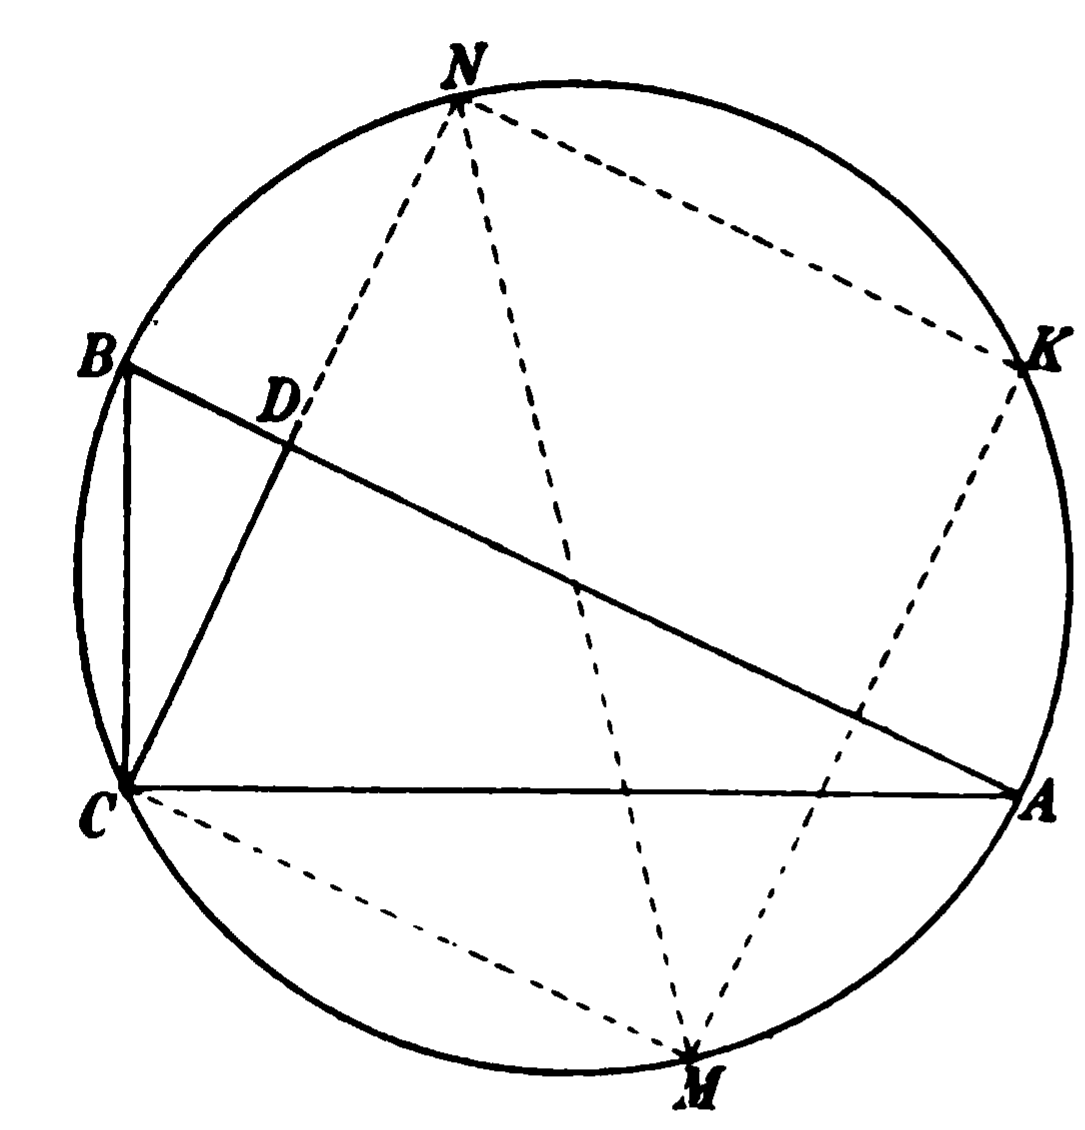
\includegraphics[width=\linewidth]{pdf244-right-triangle-construction.png}
\end{minipage}\hfill
\begin{minipage}[t]{0.57\textwidth}
(b) $ABC$ を $C$ で直角となる直角三角形とする。垂線 $CD$ を引いて斜辺を $DB$ と $DA$ の二部分に分ける。$CD$ を延長して外接円と再び $N$ で交わらせ、辺 $CN$ 上に内接長方形 $CNKM$ を完成する。このとき $MNK$ は別の直角三角形で、その二辺は $KN=DA-DB$ および $KM=2.CD$、斜辺は元の三角形 $ABC$ と同じである。いま $CB=(2m+1)$、$CA=(2n)$ と書く。このとき
\end{minipage}
\[
2.CB.CA=AB(2.CD)=2(2m+1)(2n).
\]
したがって直角三角形 $KMN$ の辺は
\[
(2n)^2-(2m+1)^2,\qquad 2(2m+1)(2n),\qquad (2n)^2+(2m+1)^2
\]
に比例し、これを求める解とする。

(c) $c=(2m+1)^2+(2n)^2$ と取る。原文ではこの後に ``souared'' と印刷されている。
\[
c^2=(2m+1)^4+2(2m+1)^2(2n)^2+(2n)^4.
\]
ここで $2(2m+1)^2(2n)^2$ の符号を変えても、結果はなお完全平方である。したがって $a=2(2m+1)(2n)$ と取ることができ、そのとき
\[
c^2-a^2=\{(2m+1)^2+(2n)^2\}^2-4(2m+1)^2(2n)^2=\{(2m+1)^2-(2n)^2\}^2,
\]
したがって $b=(2m+1)^2-(2n)^2$ である。

一〇〇〇を超えない $a$、$b$、$c$ の値は表に与えられている。

2. 三辺と面積が整数値で与えられる不等辺三角形の場合、Matsunaga は三つの方法を考察し、それらが決して十分満足なものではないと述べ、後世により簡単な方法の考案を望んでいる。

(a) \emph{Kurushima の方法}。三つの分数
\[
\frac{n_1}{d_1},\qquad \frac{n_2}{d_2},\qquad\text{および}\qquad
\frac{n_3}{d_3}=\frac{d_1d_2-n_1n_2}{n_1d_2+n_2d_1}
\]
を取る。
\scanfooter

\scanpage{0245}{第32章、印刷頁231}
最初の二つは任意に選ぶ。ただし、$n_3<n_1$、$d_3<d_1$、または $n_3<n_2$、$d_3<d_2$ となる $d$ と $n$ の値は用いてはならないと述べられている。$n_3=n_1$、$d_3=d_1$、または $n_3=n_2$、$d_3=d_2$ ならば二等辺三角形の場合となり、$n_3=d_3-1$ ならば直角三角形となる。このとき
\[
a_1=n_1(n_2d_3+n_3d_2),\qquad a_2=n_2(n_3d_1+n_1d_3),\qquad a_3=n_3(n_1d_2+n_2d_1)
\]
が三角形の三辺の値を与える。これらの値に共通因子があれば、その因子を除くべきであると述べられている。

分数 $n_1/d_1$ と $n_2/d_2$ を逆数にした場合にも同じ解法規則が適用される。この場合、新しい分母の積が分子の積より小さければ、その値を採用してはならない。

(b) \emph{ある数学者の方法}。$m>n$ である三数 $m$、$n$、$k$ を取り、
\[
A=(m^2+n^2)k,\qquad B=(m^2+n^2)n\quad\text{または}\quad(n^2+k^2)m,
\]
\[
C=(m^2-n^2)k+(n^2-k^2)m\quad\text{または}\quad(m^2-n^2)k+(m^2-k^2)n
\]
を作れば、$A$、$B$、$C$ のいずれの組も一つの解である。

(c) \emph{著者の方法}。$a_1$、$b_1$、$c_1$ と $a_2$、$b_2$、$c_2$ を、直角三角形の整数解の任意の二組とし、$c$ を斜辺とする。$a_1$、$a_2$ は奇数、$b_1$、$b_2$ は偶数と仮定する。共通斜辺 $c_1c_2$ を持ち、辺が $a'_1=a_1c_2$、$b'_1=b_1c_2$ および $a'_2=a_2c_1$、$b'_2=b_2c_1$ である直角三角形を描き、二頂点を結ぶと、辺 $a'_1$、$b'_2$ と $a'_2$、$b'_1$ を持つ二つの三角形ができる。二つの直角三角形の合わせ方を変えることにより、全部で八つの三角形が形成される。第三辺は $a_1a_2\pm b_1b_2$ および $a_1b_2\pm a_2b_1$ である。三辺の値に共通因子があるときは、これを除く。

一〇〇〇未満の三辺の実際の値が一つの表に与えられ、その後に一〇〇〇未満の原始数を与える別の表が続く。

3. 方程式 $rx^2+y^2=z^2$ は解
\[
x=2mn,\qquad y=rm^2\mathord{\sim}n^2,\qquad z=rm^2+n^2
\]
を持つ。ここで $n$ は因子 $r$ を含まないように選び、$r$ が奇数か偶数かに従って偶数または奇数とする。

4. 方程式 $r(z^2-y^2)=x^2$ の解は
\[
x=2r\times mn,\qquad y=rm^2-n^2,\qquad z=rm^2+n^2.
\]
である。
\scanfooter

\scanpage{0246}{第32章、印刷頁232}
5. 型 $rx^2-y^2=z^2$ の方程式について、Matsunaga は、解けるものもあるが解のないものもあると述べる。解かれた型では $r$ は $k^2$、$2k^2$ または $k^2+l^2$ の形である。

(a) $2x^2-y^2=z^2$ の解は
\[
x=m^2+x^2,\qquad y=(m+n)^2-2n^2,\qquad z=(m+n)^2-2m^2.
\]
である。

(b) $2k^2x^2-y^2=z^2$ の解は
\[
x=c,\qquad y=k(a\pm b),\qquad z=k(a\mp b),
\]
である。ここで $a$、$b$、$c$ はピタゴラス関係を満たす任意の整数である。

(c) $(k^2+l^2)x^2-y^2=z^2$ の解は
\[
\begin{array}{r@{\qquad}l}
(1)&x=c,\qquad y=ka\pm lb,\qquad z=la+kb;\\[1mm]
(2)&x=c,\qquad y=la\mp kb,\qquad z=ka\pm lb,
\end{array}
\]
である。ここで $a$、$b$、$c$ は前と同じであり、上または下の符号を同時に取る。

(d) $k^2x^2-y^2=z^2$ の解は $x=c$、$y=ka$、$z=kb$ である。

6. 型 $kx^2-ly^2=z^2$ の方程式は、$k-l$ が完全平方であるとき、いくつかの特別な場合に解くことができる。$x^2=\alpha^2+l\beta^2$、$y=\alpha+B\beta$ と書けば、
\[
\begin{aligned}
z^2&=k\alpha^2-ly^2=k(\alpha^2+l\beta^2)-l(\alpha+B\beta)^2\\
&=(k-l)\alpha^2-2lB\alpha\beta+l(k-B^2)\beta^2\\
&=\frac1{k-l}\left\{[(k-l)\alpha-lB\beta]^2+[(k-l)l(k-B^2)-l^2B^2]\beta^2\right\}
\end{aligned}
\]
であり、これを完全平方にしなければならない。$(k-l)l(k-B^2)-l^2B^2=0$ と置けばこれを実現でき、$B=\pm\sqrt{k-l}$ と定められる。したがって $y$ と $z$ は
\[
y=\alpha\pm\sqrt{k-l}\,\beta,\qquad z=l\beta\pm\alpha\sqrt{k-l}
\]
となる。$\alpha$ と $\beta$ の値は関係 $x^2=\alpha^2+l\beta^2$ を満たすように定めるべきである。したがって §3 から
\[
x=lm^2+n^2,\qquad \alpha=lm^2-n^2,\qquad \beta=2mn.
\]
を得る。同様に $y^2=\alpha^2-k\beta^2$、$x=\alpha+B\beta$ と書けば、
\[
x=(km^2+n^2)\pm\sqrt{k-l}(2mn),\qquad y=km^2-n^2,
\]
\[
z=\sqrt{k-l}(km^2+n^2)\pm k(2mn)
\]
を得る。

7. 方程式 $k^2x^2-ry^2=z^2$ または $rx^2-k^2y^2=z^2$ は、すでに説明した場合を適用して解くことができる。しかし $k-r$、$k$、$r$ のいずれも完全平方でない一般形 $kx^2-ry^2=z^2$ は、Matsunaga によればまだ解かれていない。
\scanfooter

\scanpage{0247}{第32章、印刷頁233}
8. $k+r$ が完全平方である方程式 $kx^2+ry^2=z^2$ を解くため、Matsunaga は上と同様の方法を適用し、
\[
y^2=\alpha^2-k\beta^2,\qquad x=\alpha+B\beta;
\]
または
\[
x^2=\alpha^2-r\beta^2,\qquad y=\alpha+B\beta
\]
と書く。

9. 方程式 $x^2+xy+y^2=z^2$ の解は
\[
x=m^2-n^2,\qquad y=(m+n)^2-m^2,\qquad z=(m+n)^2-mn
\]
と与えられる。$xy$ の符号が負のときは、$y$ と $z$ の式を交換すべきである。

10. 方程式 $x^2+y^2+z^2=u^2$ を解くため、Matsunaga は $x$ と $y$ を任意に取る。$x^2+y^2$ を二因子 $\alpha$ と $\beta$ の積に分けると、$z$ と $u$ は
\[
z=\frac12(\alpha\mathord{\sim}\beta)\qquad\text{および}\qquad u=\frac12(\alpha+\beta)
\]
によって与えられる。この考察は
\[
x_1^2+x_2^2+\cdots=y^2
\]
にも適用されるが、著者はこれを述べていない。

11. 方程式 $x^2+y^2=z^3$ の解は
\[
x=(m^2\mathord{\sim}3n^2)m,\qquad y=(3m^2\mathord{\sim}n^2)n,\qquad z=m^2+n^2.
\]
である。

12. $x^3+y^3+z^2=u^4$ の解は
\[
x=m^4-n^4,\qquad y=4m^2n^2,\qquad z=2(m^2-n^2)mn,\qquad u=m^2+n^2.
\]
である。ここで著者は、四要素を超える場合に適用できる方法はまだ見いだされていないと付記する。

13. $x^2-y^2=z^4$ の解は
\[
x=m^4-n^4,\qquad z=m^2-n^2,\qquad y=2mnz.
\]
である。

14. 方程式 $x^3-y^3=z^4$ の解は
\[
z=m^3-n^3,\qquad x=zm,\qquad y=zn.
\]
である。

15. 方程式 $x^2+y^2=k$ を解くため、$\frac12k=r^2+R$ とし、$r^2$ を $k$ に含まれる最大の平方数とする。量
\[
a_1=2r-1,\qquad a_2=a_1-2,\qquad a_3=a_2-2,\qquad a_4=a_3-2,\ldots,
\]
\[
b_1=2r+1,\qquad b_2=b_1+2,\qquad b_3=b_2+2,\qquad b_4=b_3+2,\ldots
\]
を作り、$2R=A$ から $b_1$、$b_2$、\ldots を逐次引く。これらの減算が不可能なら、$a_1$、$a_2$、\ldots を逐次加えて減算を行う。最後に余りが消えるところに達したなら、最後に用いた $a$ と $b$ の値を $a'$ と $b'$ とする。このとき
\[
x=\frac12(a'+1)\qquad\text{および}\qquad y=\frac12(b'-1)
\]
が求める解である。
\scanfooter

\scanpage{0248}{第32章、印刷頁234}
別解。$k=r'^2+R'$ とし、
\[
a'_1=2r'-1,\qquad a'_2=a'_1-2,\qquad a'_3=a'_1-4,\qquad a'_4=a'_1-6,\ldots
\]
と書く。$R$ から $1$、$3$、$5$、\ldots を、これ以上演算を続けられなくなるまで逐次引く。最後の余りを $A'$、最後の減数を $b'_1$ とする。そして
\[
b'_2=b'_1+2,\qquad b'_3=b'_1+4,\qquad b'_4=b'_1+6,\ldots
\]
と書き、第一の方法と同じように進める。これにより同様に必要な $x$ と $y$ の値を得ることができる。

16. 方程式 $a^2+bx=y^2$ を解くには、$b$ を二因子 $mn$ の積に分け、関係 $mp-nq=1$ を満たす数 $p$ を求める。$2pa\equiv A\pmod n$ となる数 $A$ を求める。このとき $x=\frac1nA(Am-2a)$ が求める値である。$Am-2a=0$ なら、$A$ の代わりに $A+n$ を取り、同様に進める。$A=0$ なら $A$ として $m$ を取る。$Am-2a<0$ なら、$Am-2a$ の代わりに $(A+1)m-2a$ を取らなければならない。

また別に、$2a+b$ を $bQ+R$ の形に書けば、$x=(2a+b)-(Q+1)R$ が答となる。この方法は $b$ が素数であるとき有利に適用できると記されている。しかし逆の場合には、あまり小さくない $x$ の値を導く。

17. 方程式 $a+bx=y^2$、たとえば $69+11x=y^2$ を解くため、まず
\[
1=1^2\equiv\alpha_1,\qquad 1+3=2^2\equiv\alpha_2,\qquad 1+3+5=3^2\equiv\alpha_3,\ldots
\]
を作る。法は $b=11$ である。$\alpha$ の数は明らかに一定数に限られる。この場合には $\alpha_1=1$、$\alpha_2=4$、$\alpha_3=9$、$\alpha_4=5$、$\alpha_5=3$ だけを取ればよい。すると
\[
\frac ab=Q+\frac Rb=6+\frac3{11}
\]
である。$R=3$ と $\alpha$ を比較すると、$R$ は $(\alpha_r=)\alpha_5$ に等しい。$R$ に等しい $\alpha$ がなければ、問題は解けない。次に
\[
2\times r+b=21=1\times b+10=Q'b+R',
\]
\[
(2r+b)-(Q'+1)R''=1=K,\qquad Kb+r^2=36=6^2=k^2,
\]
\[
k+b=23=bQ''+R''=b\times2+1
\]
を作る。
\scanfooter

\scanpage{0249}{第32章、印刷頁235}
\[
(k+b)-(Q''+1)R''=23-3\times1=20=h,
\]
\[
h\times b+k^2=256,\footnote{この量が $<a$ なら、すでに行ったように、さらに手続を反復する必要がある。}\qquad \frac{256-a}{b}=17,
\]
そしてこの最後の量が求める $x$ の値である。

18. 「\emph{問題}。まだ未知であるある数がある。これを加法的な一次係数 69 とともに二次へ展開すれば、余り 15 が残る。加法量 72 とともに同じことをすれば、余りは 7 となる。未知数はいくつか。」

ここでは用いられた術語の意味を逐語的に訳したため、旧日本数学者の独特な記述法に慣れていない読者にはほとんど理解できないであろう。しかし記号的に表せば、この問題は方程式
\[
y_1^2+69y_1=x-15,\qquad y_2^2+72y_2=x-7,
\]
また一般には
\[
y_1^2+a_1y_1=x-b_1,\qquad y_2^2+a_2y_2=x-b_2
\]
を満たす $x$ の整数値を求めることにほかならない。

Matsunaga はこの問題を次のように解く。量
\[
(a_2^2+4b_1)\mathord{\sim}(a_1^2+4b_2)=455
\]
を $mn$ に因数分解し、$m$ と $n$ は $m+n\geq2a_1$ または $2a_2$ となるように選ぶ。この場合、二因子 91 と 5 は採用できないので、$m=455$、$n=1$ と取らなければならない。すると
\[
\frac12\left(\frac{m-n}{2}-a_1\right)=79=y_1,
\qquad
\frac12\left(\frac{m+n}{2}-a_2\right)=78=y_2,
\]
となり、$x$ の値は直ちに 11707 と得られる。

$\frac12(m-n)-a_1<\frac12(m+n)-a_2$ の場合には
\[
y_1=\frac12\left(\frac{m+n}{2}-a_1\right),
\qquad
y_2=\frac12\left(\frac{m-n}{2}-a_2\right)
\]
と取る。

この規則の解析は次のように試みられる。与えられた二関係から $x$ を消去すると
\[
(-b_2+b_1+a_1y_1+y_1^2)-a_2y_2-y_2^2=0
\]
を得、そこから
\[
y_2=-\frac{a_2}{2}+\frac12\sqrt{a_2^2+4(-b_2+b_1+a_1y_1+y_1^2)}
\]
が従う。ここで根号内の量を $k_2^2$ で表し、これを $y_1$ について解くと（文字 $l$ を用いる）、
\[
y_1=-\frac{a_1}{2}+\frac12\sqrt{a_1^2+4b_2-a_2^2-4b_1+k_2^2}
=-\frac{a_1}{2}+\frac12l
\]
となる。
\scanfooter

\scanpage{0250}{第32章続き、印刷頁236}
ここで $a_1^2+4b_2-a_2^2-4b_1$ の数値を $\pm mn$ とする。$l^2$ が完全平方となるためには、$l$ は $\frac12(m\pm n)$ の形でなければならない。したがって
\[
y_1=\frac12\left(\frac{m\pm n}{2}-a_1\right),
\qquad\therefore\qquad
k^2=\left(\frac{m\pm n}{2}\right)^2\mp mn=\left(\frac{m\mp n}{2}\right)^2,
\]
を得、したがって $y_2$ の値は
\[
\frac12\left(\frac{m\mp n}{2}-a_2\right)
\]
となる。

19. 方程式 $a+cx=(b+dx)y$ を解くため、Matsunaga はこれを $(a-by)+(c-dy)x=0$ の形に書き直し、$x$ の方程式として考える。$x$ の係数が未知量を含まなければ、\emph{jōichi jutsu}、すなわち関係 $mp-nq=1$ を適用できる。絶対項が未知量を含まなければ、この項を因数分解して解くことができる。しかしここでは $x$ の係数と絶対項の双方が、なお未知である $y$ に依存するため、いずれも直接には適用できない。ところが $x=x_1/d$ と書けば、方程式は
\[
(ad-bdy)+(c-dy)x_1=0
\]
となり、置換 $x_1=x_2-b$ を行えば
\[
(ad-bd)+(c-dy)x_2=0
\]
を得る。これにより絶対項が $y$ に依存しない形になる。$x$ は正でなければならないから、$x_1$ も正でなければならず、したがって $x_2-b>0$、すなわち $x_2>b$ で、必然的に正である。ゆえに最後の方程式の二係数は異符号である。そこで
\[
mn\pm(c-dy)x_2=0
\]
と書く。二符号は事情による。ここでは $m=x_2$、$n=\mp(c-dy)$ と取ればよく、後者は必ず正でなければならない。$x$ と $y$ の値は直ちに従う。

20. 上に述べたところでは、数の因数分解がしばしば用いられた。この問題に対する Matsunaga の試みは次のとおりである。因数分解すべき数を $r^2+R$ の形に書き、まず $r$ が奇数の場合を考える。
\[
r=B_1,\qquad B_1-2=B_2,\qquad B_2-2=B_3,\qquad B_3-2=B_4,\ldots
\]
と書けば、次の計算を行う。
\[
\begin{array}{rcl@{\qquad}rcl@{\qquad}rcl}
R&=&Q_1B_1+A_1,&K_1&=&2Q_1,&K'_2&=&K_1+4,\\
A_1+K'_2&=&Q_2B_2+A_2,&K_2&=&2Q_2+K'_2,&K'_3&=&K_2+8,\\
A_2+K'_3&=&Q_3B_3+A_3,&K_3&=&2Q_3+K'_3,&K'_4&=&K_3+8,\\
A_3+K'_4&=&Q_4B_4+A_4,&K_4&=&2Q_4+K'_4,&K'_5&=&K_4+8,
\end{array}
\]
\[
\cdots\cdots\cdots\cdots\cdots\cdots\cdots\cdots\cdots
\]
\scanfooter


\scanpage{0251}{第32章結末および第33章、印刷頁237}
これは、$A_n$ の値が零となるところに到達したとき終わる。この場合、$B_n$ の値が求める因数である。他の因数は $\frac12K_n+B_n+2$ によって与えられる。

$r$ が偶数である場合には、$r-1=B_1$ と書き、$R$ の代りに $R+1$ を取り、他の場合と同じ仕方で進めなければならない。

これらの計算では、二段または三段を一つの演算にまとめることによって労力を省けるが、その仕方は容易に従うであろう。

\begin{center}
第33章。\\[1mm]
不定方程式 $x^n-ky=a$。
\end{center}
\phantomsection\addcontentsline{toc}{subsection}{第33章　不定方程式 $x^n-ky=a$ }

一八世紀前半に属すると思われる、あるいは確実に属する無名写本があり、題を \emph{Ruijō Ruiyaku Shinjutsu} といい、その中で不定方程式 $x^n-ky=a$ が解かれている。そのため、未知の著者は次の合同式を作る。
\[
1^n\equiv1\equiv a_1,\qquad 2^n\equiv a_2,\qquad 3^n\equiv a_3,\ldots,\qquad (k-1)^n\equiv a_{k-1},
\]
法は $k$ である。次に、量 $a_1,a_2,\ldots,a_{k-1}$ の中から与えられた数 $a$ に等しいものを選び、それを $a_r$ とする。著者はここで $x=r$ を、求める $x$ の値とする。

上の合同式を作る際には、いくつかの工夫によって相当量の労力を省くことができる。すなわち、$k$ が偶数または奇数であるのに従って、$a_{k-r}=a_r$ または $k-a_r$ となる。これは次のように証明できる。\footnote{ここでは $(M)$ を「ある倍数」の意味に書く。}
\[
\begin{aligned}
(k-r)^n&=(M)k+(-1)^nr^n=(M)k+(-1)^n\{(M)k+a_r\}\\
&=(M)k+(-1)^na_r=(M)k+a_r\quad\text{または}\quad(M)k+(k-a_r).
\end{aligned}
\]
また $a_r$ を求めるには、$r$ の $n$ 乗を直接作る必要はない。次のように進めるのが有利である。
\[
r^2\equiv b_1,\qquad r^3\equiv b_1r\equiv b_2,\qquad r^4\equiv b_2r\equiv b_3,\ldots,\qquad r^n\equiv b_{n-2}r\equiv a_r.
\]
$r$ が $r_1r_2r_3\cdots$ の形であるときには、その積が求める $r$ の剰余を与える各因数の剰余を用いることができる。

例として方程式 $x^5-29y=25$ を取る。ここで $a_1,a_{28};a_2,a_{27};\ldots$ は次の値をもつ。
\[
\begin{array}{rrrrrrrrrrrrrr}
1&3&11&9&22&4&16&27&5&8&14&12&6&19\\
28&26&18&20&7&25&13&2&24&21&15&17&23&10
\end{array}
\]
この表では数 25 が $a_{23}$ によって与えられる。したがって求める $x$ の値は $x=23$ である。
\scanfooter

\scanpage{0252}{第34章冒頭、印刷頁238}
\begin{center}
第34章。\\[1mm]
AJIMA の \emph{RENJUTSU HENKAN}。
\end{center}
\phantomsection\addcontentsline{toc}{subsection}{第34章　AJIMA の RENJUTSU HENKAN }

一七八四年第三月、Ajima Chokuyen は \emph{Renjutsu Henkan} と題する写本を書いた。この題は、おそらく「一般的考察を類似した性質の諸場合へ適用すること」と訳せよう。これは \emph{tenzan} 代数の発達が到達した最高水準を示す成果の一つであった。書物の内容は、本質的には以下に再現する通りである。

\begin{center}
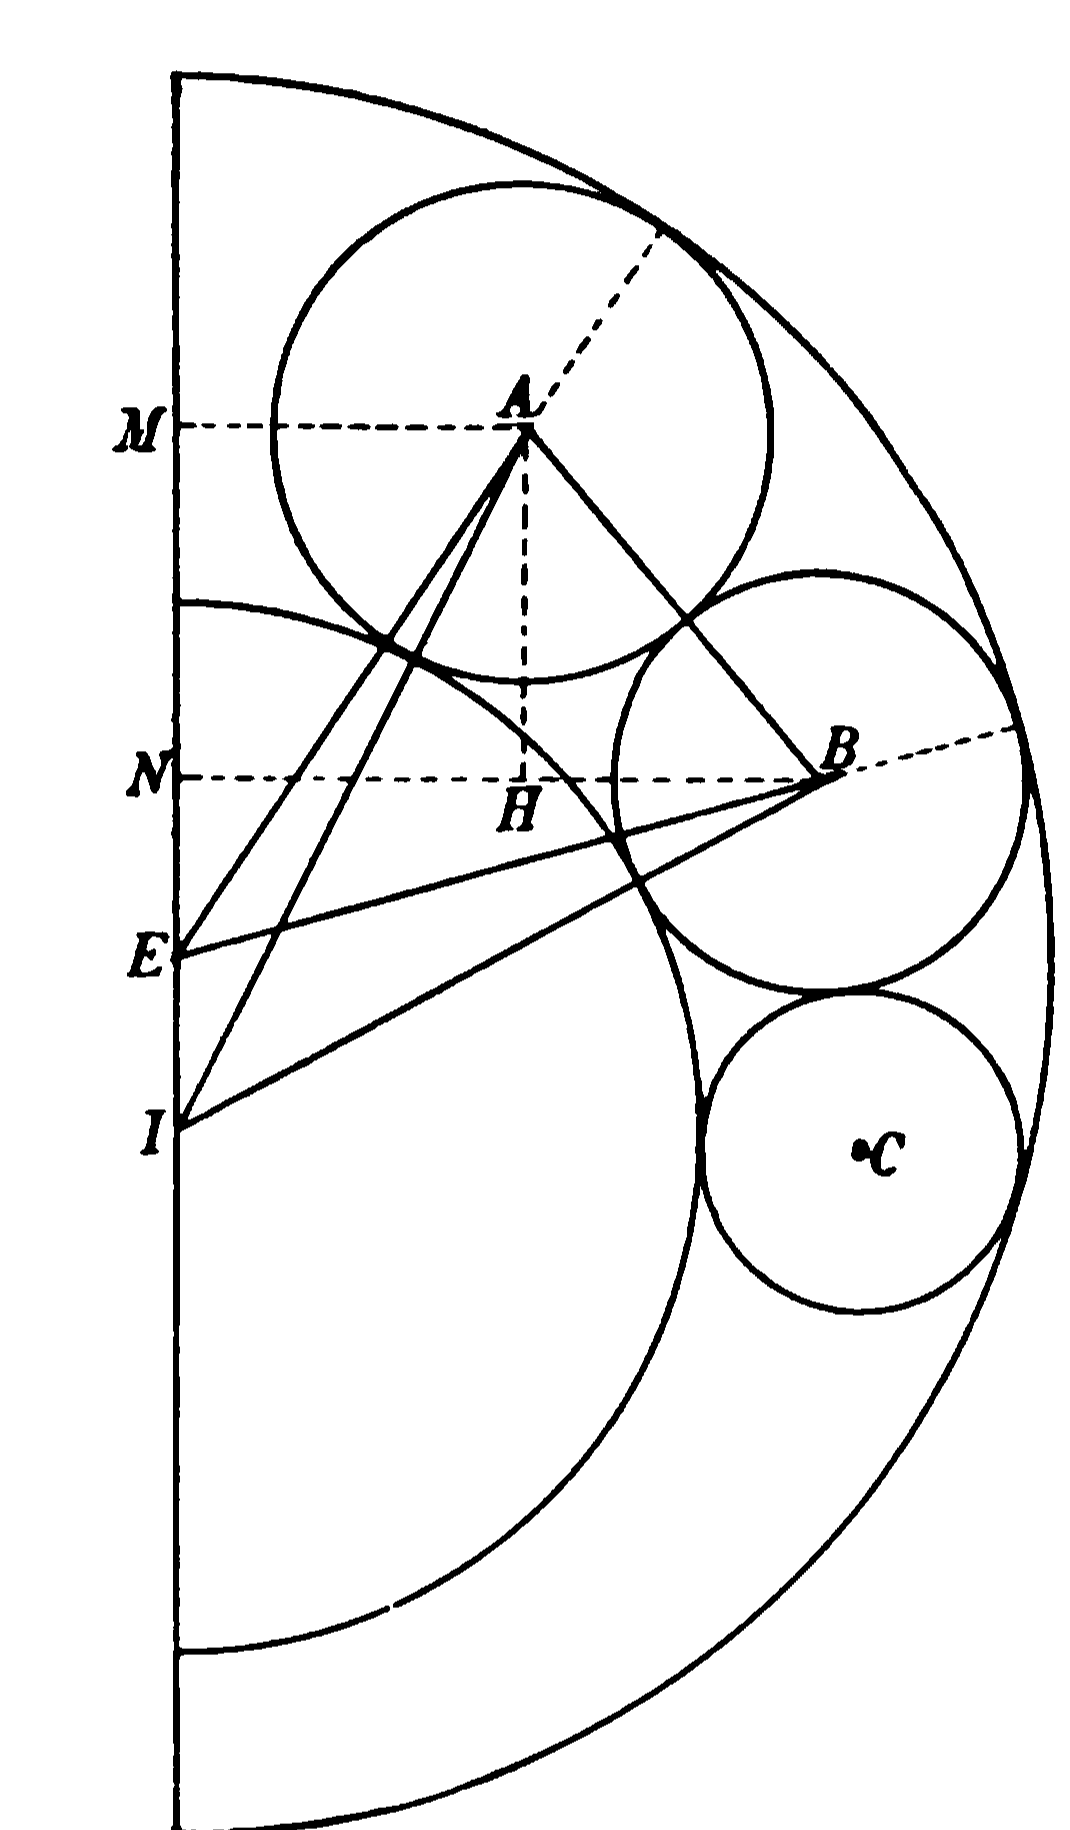
\includegraphics[width=0.48\linewidth]{pdf252-renjutsu-three-circles.png}
\end{center}

1. 図において $E$ を外円、$I$ を内円とする。三円 $A,B,C$ は、この二円および互いに接するように描かれている。これらの文字は各円の中心を表すと同時に、その直径も表す。$I,E,B$ および矢 $s$ によって $A$ と $C$ を求めることが要求される。ここで $s$ は、$E$ と $I$ の共通直径上で二円周の間に含まれる部分である。

次のように書く。
\[
\begin{gathered}
a=2\dd\overline{IE}=-E+I+2s,\qquad b=2\dd\overline{EA}=E-A,\\
c=2\dd\overline{IA}=I+A,\qquad d=2\dd\overline{EB}=E-B,\\
e=2\dd\overline{IB}=I+B,\qquad f=2\dd\overline{AB}=A+B.
\end{gathered}
\]
また $AM$ と $BN$ を $IE$ に直角に引き、$AH$ を $BN$ に直角に引いて、$g=2\dd EM$, $h=AM$, $i=2\dd EN$, $j=BN$, $k=2\dd AH$, $l=BH$ と書く。このとき\footnote{本文中の諸式は、写本ごとに異なっているため、あまり信頼できない。しかし私は必ずしもそれらを訂正しようとはしなかった。解析の主要な特徴を示すことができれば、私の目的は達せられるからである。}
\[
ag=\frac12(c^2-a^2-b^2),\qquad\text{および}\qquad a^2h^2=\frac14(a^2b^2-a^2g^2),
\]
である。整理し、$m=E\dd I+Es-Is-s^2$ と書けば、
\[
a^2h^2=m\{(E-I)s+s^2+(E-I)A-A^2\}
\]
を得る。同様に
\[
a^2j^2=m\{-(E-I)s+s^2+(E-I)B-B^2\},
\]
\scanfooter

\scanpage{0253}{第34章、印刷頁239}
さらに
\[
a^2l^2=m(-A^2+2AB-B^2)+(E+I)AB,
\]
\[
\begin{aligned}
a^2j\times2l&=a^2l^2+a^2j^2-a^2h^2\\
&=m\{-2AB-2B^2-(E-I)A+(E-I)B\}+(A+B)^2AB.
\end{aligned}
\]
ここで $a^2j^2\times2l$ の平方を、$a^2j^2$ と $a^2l^2$ の積の四倍に等置し、整理して因数 $a^2$ を除くと、方程式
\[
\alpha\equiv
\left\{
\begin{aligned}
&\{(I+E)^2B^2+m^2-2m(E-I)B\}x^2\\
&+\{-2m(E-I)B^2-2mnB+2m(E-I)Bs\}x+m^2B^2
\end{aligned}
\right\}=0
\]
を得、これから $A$ を決定する。ここで $n=EI+s^2$ と書いた。$A$ を $B$ に、$B$ を $C$ に変えれば $C$ の方程式を得る。しかし、この変更によって方程式は変わらない。したがって $A$ と $C$ は上の方程式の二根である。

もし
\[
\beta=\{(E-I)B+n-(E-I)s\}x-mB
\]
と書けば、\footnote{$\alpha=0$ だからである。}
\[
\beta^2=\beta^2-\alpha=\{4IE(B+s)(B-s)-4IE(E-I)(B-s)\}x^2.
\]
したがって右辺の $x^2$ の係数を $\gamma^2$ で表し、両辺の平方根を取れば
\[
\{(E-I)B+n-(E-I)s\mp\gamma\}x-mB=0
\]
を得る。上の符号は $A$ に、下の符号は $C$ に属する。

この $A$ と $C$ の二式にそれぞれ $C$ と $A$ を掛けて加えると、
\[
\{-mB+2(E-I)BC+2nC-2(E-I)sC\}x-mBC=0
\]
を得る。これは $B$ と $C$ によって $A$ を与える。この式を基本方程式と呼ぶ。

2. 次に Ajima は、図のように描かれる円 $A_2,A_3,\ldots$ の直径を、$E,I,A_1$ によって求める。

\begin{center}
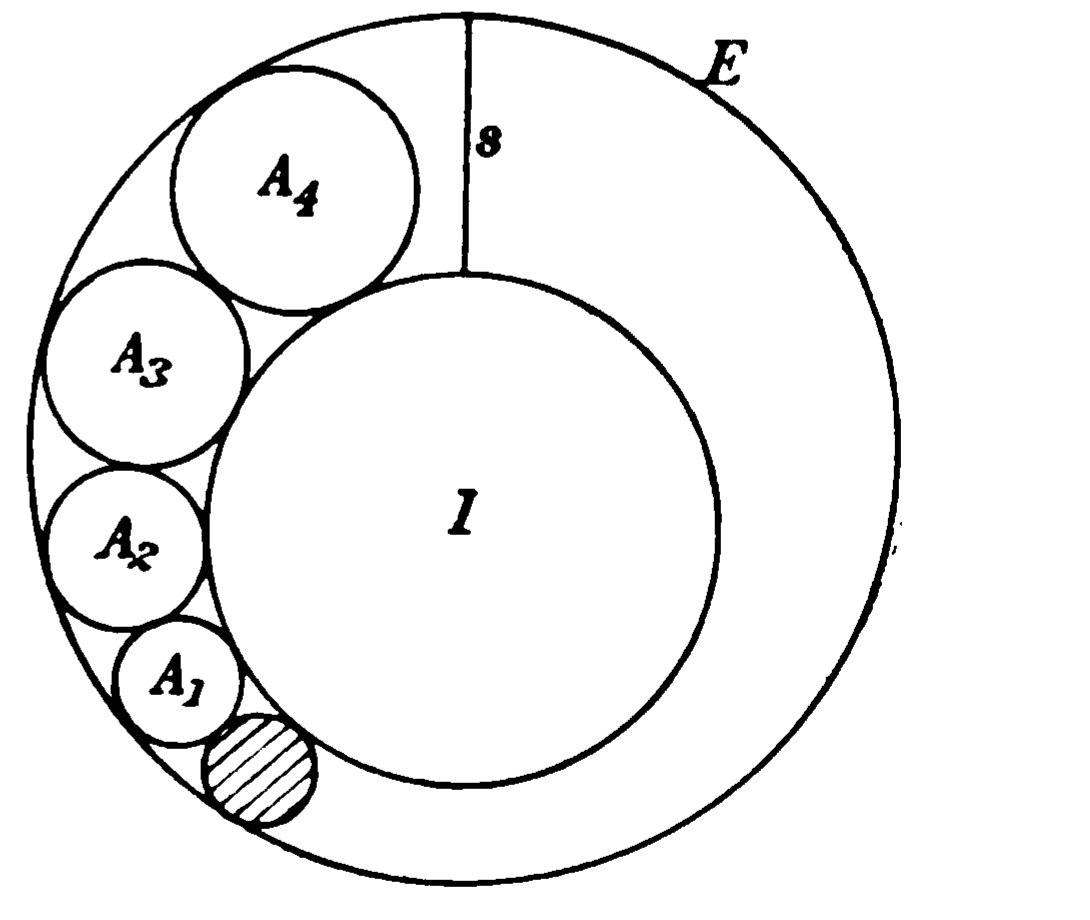
\includegraphics[width=0.40\linewidth]{pdf253-successive-circles.png}
\end{center}

ここで斜線を施した円は先に考えた場合の円 $C$ に対応し、円 $A_1,A_2$ はそれぞれ $B,A$ に対応する。したがって、すでに得た関係から、$x=A_2$ として
\[
\{(E-I)A_1+2EI-m-p\}x-mA_1=0,
\]
\scanfooter

\scanpage{0254}{第34章、印刷頁240}
ここで
\[
m=IE+Es-Is-s^2=(E-s)(I+s),
\]
\[
p=2\sqrt{(A_1+s)(A_1-s)IE-(E-I)(A_1-s)IE}
\]
と書く。さらに基本方程式で $C$ の代りに $A_1$、$B$ の代りに $A_2$ を代入すると、
\[
\{-mA_2+2(E-I)A_1A_2+2nA_1-2(E-I)sA_1\}x-mA_1A_2=0
\]
を得る。ここから $x=A_3$ を決定する。ここで $n$ は $EI+s^2$ を表す。この方程式は
\[
\left\{-1+\frac{2(E-I)A_1}{m}+\frac{4EIA_1}{A_2m}-\frac{2A_1}{A_2}\right\}x-A_1=0
\]
の形に書け、第二基本方程式と呼ばれる。

もし
\[
\frac{A_1}{A_1}=1=\rho_1,\qquad \frac{A_1}{A_2}=\rho_2,\qquad \frac{A_1}{A_3}=\rho_3,\ldots
\]
と書けば、方程式は
\[
(-\rho_1+\rho+\rho_2k)x-A_1=0
\]
となる。ここで
\[
k=\frac{4EI}{m}-2,\qquad \rho=\frac{2(E-I)A_1}{m},
\]
したがって
\[
\rho_3=\rho_2k+\rho-\rho_1,
\qquad A_3=A_1/\rho_3.
\]
第二基本方程式で $A_1$ の代りに $A_2$、$A_2$ の代りに $A_3$ を代入すれば、$A_4$ の方程式
\[
\left\{-1+\frac{2(E-I)A_2}{m}+\frac{4EIA_2}{mA_3}-\frac{2A_2}{A_3}\right\}x-A_2=0
\]
を得る。これは第三基本方程式と呼ばれる。これに $\rho_2$ を掛けると
\[
\left\{-\rho_2+\frac{2(E-I)A_1}{m}+\frac{4EIA_1}{A_3m}-\frac{2A_1}{A_3}\right\}x-A_1=0,
\]
すなわち
\[
(-\rho_2+\rho+k\rho_3)x-A_1=0
\]
となる。ゆえに
\[
\rho_4=\rho_3k+\rho-\rho_2,
\qquad A_4=A_1/\rho_4.
\]
同様に進めれば、$\rho_5,\rho_6,\ldots$ の値が順次得られる。すなわち
\[
\rho_i=\rho_{i-1}k+\rho-\rho_{i-2},
\qquad A_i=A_1/\rho_i.
\]
この関係は数学的帰納法によって証明できるが、旧日本の数学者はそのような証明法をもたなかった。この種の場合には、最初の少数の場合に成立することから、その関係を当然のものとして採用するのが慣例であった。
\scanfooter

\scanpage{0255}{第34章、印刷頁241}
3. $A_1$ が $s$ と一致するとき、$\rho_1=1$ であり、
\[
1\times k+\rho-\rho_2=\rho_2,
\qquad \therefore\quad \rho_2=\frac{k+\rho}{2};
\]
また $\rho_3,\rho_4,\ldots$ についても上に与えた同じ諸式が適用される。

4. 円 $A_1$ が $s$ に接するとき、直径 $A_1$ はまず
\[
(E+I)^2x^2-4m(E-I)x+(4m^2-4mEI)=0
\]
から求められる。これは第1節の $B$ による $A$ の二次方程式から得られる。

5. Ajima の考察は、内円が外円の内部に完全にある単純な場合に必ずしも限定されない。彼は、外円と交わる「内」円が無限大になる場合まで取り上げる。彼は次のようにいう。

「内円が限りなく大きくなると、その円周は次第に伸び、ついには直線となる。この場合、内円の直径の長さはわれわれの方法では測定できず、その大きさには限界がない。この場合の図は添付の通りである。この図は円弓であり、その内部には逐次円の列が内接している。いま問題は、外円直径 $E$、矢 $s$、円 $A_1$ の直径によって、これらの円の直径を求めることに帰着する。」（原文には \emph{whithin} とある。）

\begin{center}
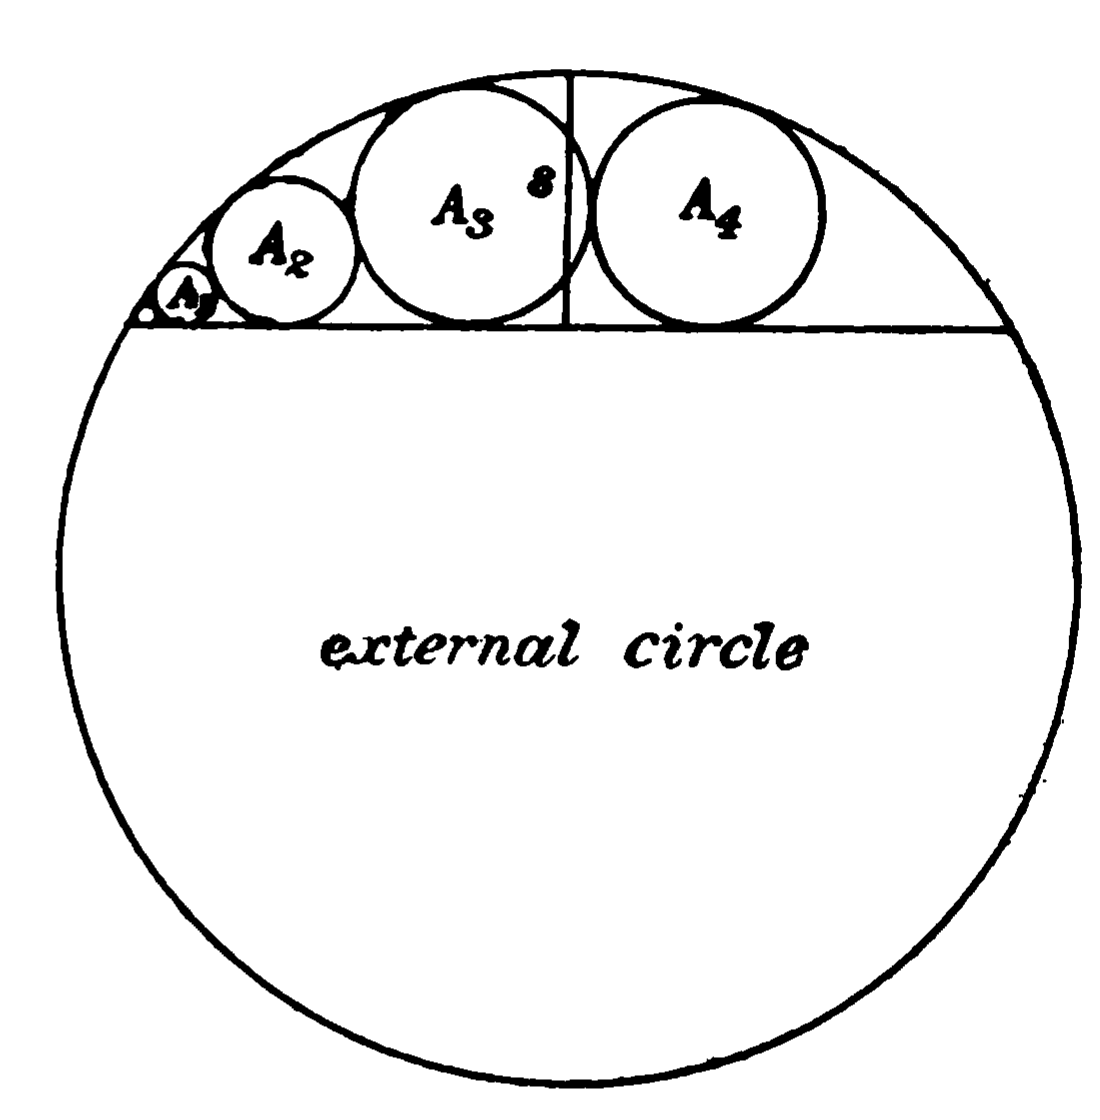
\includegraphics[width=0.44\linewidth]{pdf255-segment-inscribed-circles.png}
\end{center}

Ajima の考察によれば、ここで
\[
m=(E-s)(I+s),\qquad k=\frac{4EI}{(I+s)(E-s)}-2,\qquad \rho=\frac{2(I-E)A_1}{(I+s)(E-s)},
\]
したがって極限 $I=\infty$ では
\[
m=(E-s)\times(\text{infinity}),\qquad k=\frac{4E}{E-s}-2,\qquad \rho=\frac{2A_1}{E-s}.
\]
$\rho_2$ を求めるため、Ajima は第1節で得た方程式
\[
\{(I+E)^2B^2+m^2-2m(E-I)B\}A^2
+\{-2m(E-I)B^2-2mnB+2m(E-I)Bs\}A+m^2B^2=0
\]
を取り、$A=A_1$, $B=A_2$ と書き、$m,n$ をその値で置き換え、$(I+E)^2$ で割って $I=\infty$ の極限へ進む。その結果は
\[
\begin{aligned}
&A_1^2A_2^2+2(E-s)A_1^2A_2+2(E-s)A_1A_2^2-2(E-s)sA_1A_2\\
&\qquad{}-2(E-s)EA_1A_2+(E-s)^2A_1^2+(E-s)^2A_2^2=0,
\end{aligned}
\]
\scanfooter

\scanpage{0256}{第34章、印刷頁242}
これは円弓に内接する円の方程式と呼ばれる。これは $A_2$ について二次であり、第1節と同様に扱えば
\[
\{-A_1+E+s\mp\sqrt{E(s+A_1)}\}x-(E-s)A_1=0
\]
を得る。上の符号は $A_2$ に、下の符号は $A_1$ の反対側の円に属する。$E-s$ で割れば、$A_2$ について
\[
\frac1{E-s}\{-A_1+E+s-2\sqrt{E(s+A_1)}\}x-A_1=0
\]
となり、これから $\rho_2$ を得る。以前と同様に、$\rho_3,\rho_4,\ldots$ を求め、それによって $A_2,A_3,A_4,\ldots$ を得られる。

6. 円 $A_1$ が矢 $s$ を直径として描かれる場合、または $A_1$ が円弓の矢に接する場合は、前節で得た一般式の特殊な場合として扱うことができる。

7. 外円と内円が互いに接するとき、
\[
s=E-I,\qquad E-s=I,\qquad I+s=E,\qquad m=IE,\qquad n-(E-I)s=IE,
\]
したがって $A_2$ の方程式は
\[
\{I^2E^2-2(E-I)IEA_1+(E+I)^2A_1^2\}x^2
+\{-2I^2E^2A_1-2(E-I)IEA_1^2\}x+I^2E^2A_1^2=0
\]
となる。これを解けば
\[
\left\{1+\frac{(E-I)A_1}{EI}-\sqrt{\frac{4(E-I)A_1}{EI}-\frac{4A_1^2}{EI}}\right\}x-A_1=0
\]
を得、その $x$ の係数が $\rho_2$ の値を与える。$\rho$ と $k$ については
\[
\rho=\frac{2(E-I)A_1}{m}=\frac{2(E-I)A_1}{IE},\qquad k=\frac{4IE}{m}-2=2,
\]
であり、これらによって $\rho_3,\rho_4,\ldots$ の値を決定する。

8. いま考えた場合の外円が無限大になるとする。この場合、外円は伸びて直線となる。ここでは $A_1$ は必然的に $A_2$ より大きいので、$A_2$ の決定には、根号の前に正符号を取った方程式
\[
\left\{1+\frac{(E-I)A_1}{EI}+\sqrt{\frac{4(E-I)A_1}{EI}-\frac{4A_1^2}{EI}}\right\}x-A_1=0
\]
を採用する。極限 $E=\infty$ に進むと、これは
\[
\left(1+\frac{A_1}{I}+\sqrt{\frac{4A_1}{I}}\right)x-A_1=0,
\]

\begin{center}
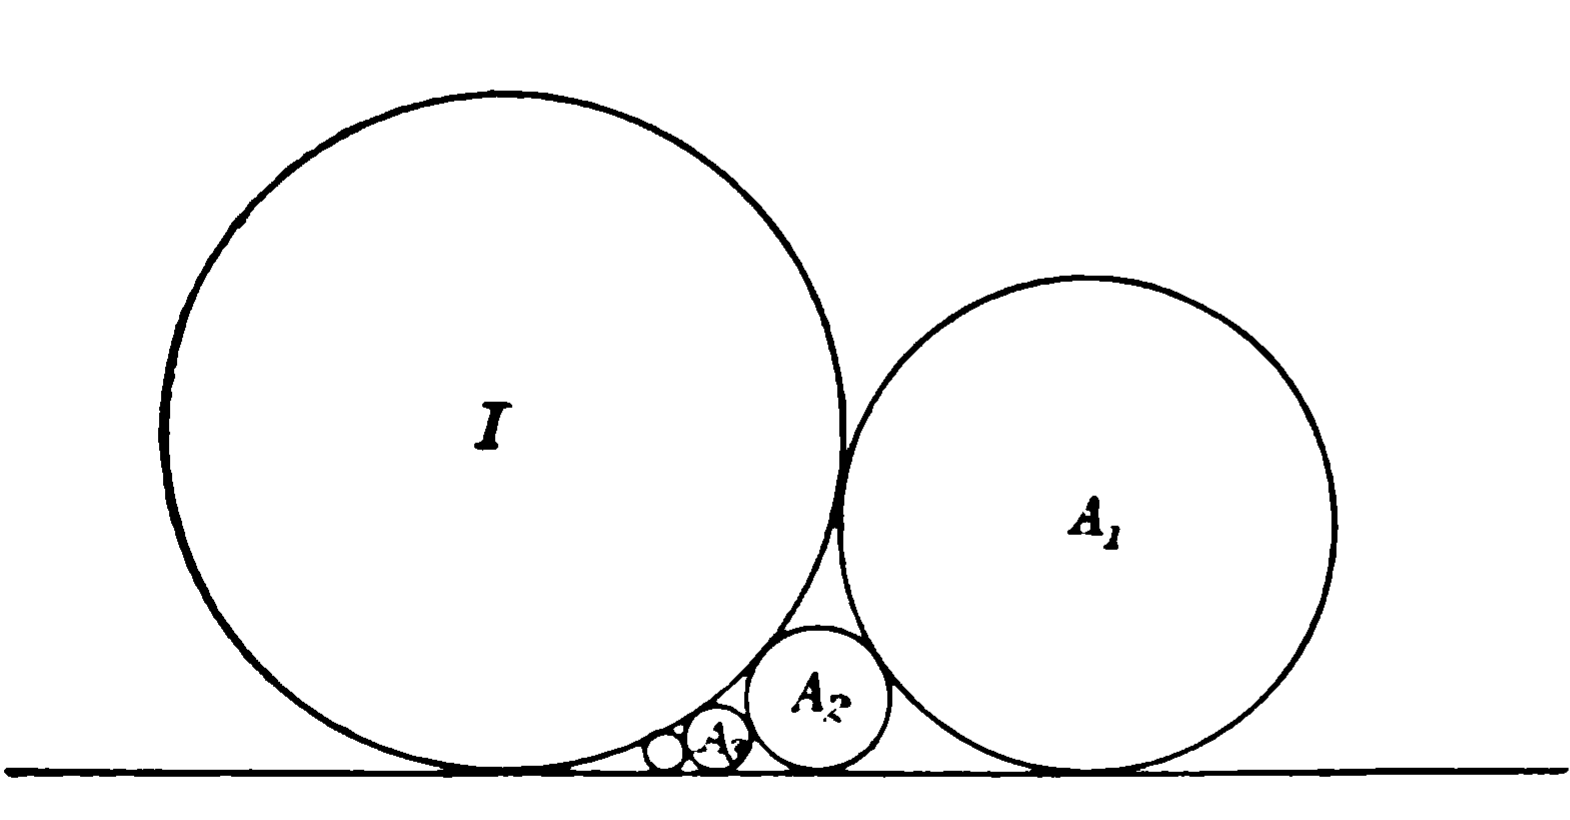
\includegraphics[width=0.56\linewidth]{pdf256-line-tangent-successive-circles.png}
\end{center}
\scanfooter

\scanpage{0257}{第34章結末および第35章冒頭、印刷頁243}
となり、これから $\rho_2$ と $A_2$ を得る。ここで $\rho$ と $k$ は
\[
\rho=\frac{2(E-I)A_1}{EI}=\frac{2A_1}{I},\qquad k=2
\]
であり、$\rho_3,\rho_4,\ldots$ の値を決定するのに用いられる。

9. Ajima は著作を次の言葉で結ぶ。「前の論考で考えた事柄のほかにも、性質が互いに似た一群の問題に出会うときは、まず一般の場合を論じ、次いでその結果を類似の場合に変えることによって、同様に進むことができる。ここでは例として \emph{renjutsu} の一場合だけを選び、論じた。」

したがって Ajima が \emph{renjutsu} という語によって意味したのは、特殊な場合に適用できる一般的考察であったことがわかる。旧日本数学者の考察は常に特殊的で一般性を欠いたと普通信じられているが、この写本の内容を調べると、その信念は、創造的天才で特に名高い Ajima Chokuyen には当てはまらないと感じられる。

\begin{center}
第35章。\\[1mm]
一円内で冠状をなす逐次内接円に関する AJIMA の研究。
\end{center}
\phantomsection\addcontentsline{toc}{subsection}{第35章　一円内で冠状をなす逐次内接円に関する AJIMA の研究}

1. 前章では、一七八四年の写本に記された、外円と内円の間に逐次内接する円に関する Ajima の研究に触れた。同じ問題で、内接円が図のように環をなす場合も彼によって研究された。ここでは二つの写本、\emph{Yennai Yō-Ruiyen-Jutsu} および \emph{Yennai Yō-Ruiyen-Jutsu Kōhen}（円内の逐次内接円、およびその続編）に記された Ajima の結果について述べる。前者は一七八四年第二月改訂、後者は一七九一年第六月改訂と記されている。したがって前者は、前章で述べた写本より前に書かれた。

\begin{center}
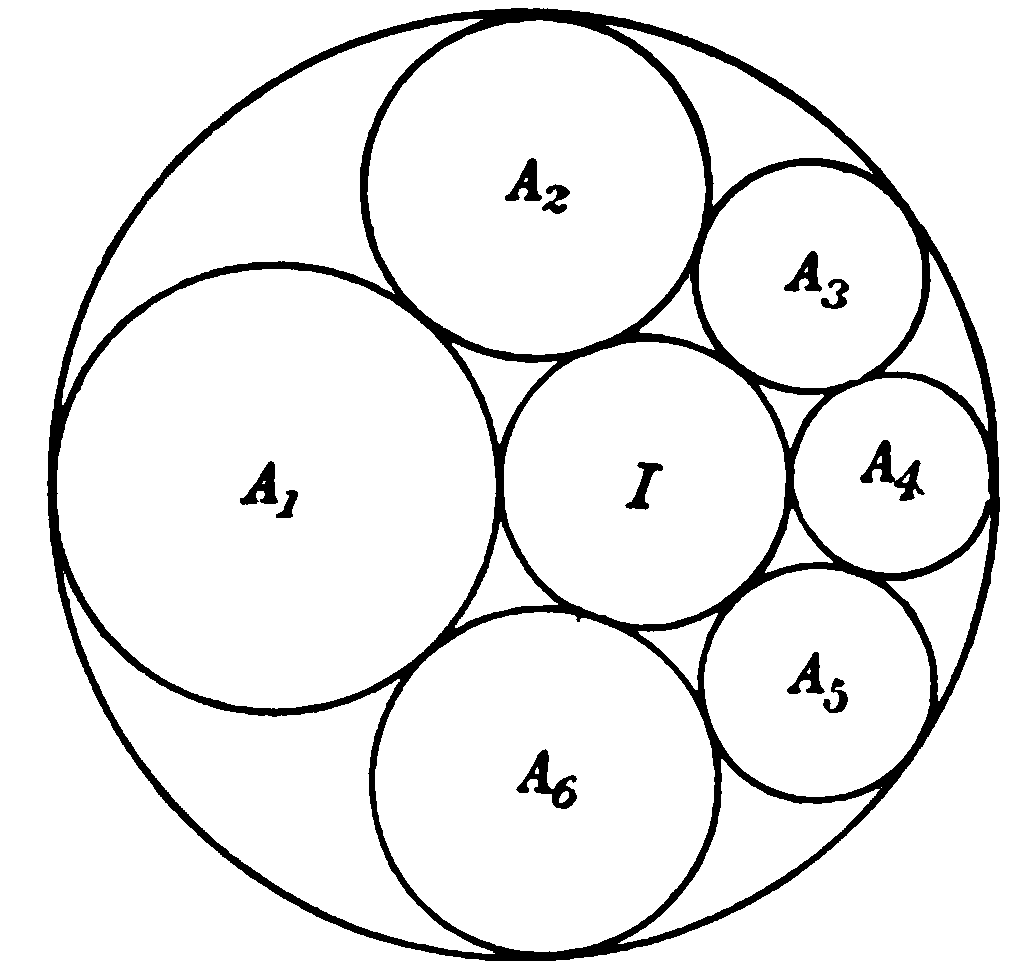
\includegraphics[width=0.42\linewidth]{pdf257-crown-inscribed-circles.png}
\end{center}

2. 一七八四年の写本で Ajima はまず、円 $A_1$ が外円と
\scanfooter

\scanpage{0258}{第35章、印刷頁244}
内円、すなわち $E$ と $I$ の「矢」のまわりに描かれる場合を考える。この矢は、両円に共通な直径のうち、その二円周によって切り取られた部分である。この場合、
\[
\rho_2=A_1/A_2,\qquad \rho_3=A_1/A_3,\ldots
\]
および
\[
t=\frac{4EI}{(I+A_1)(E-A_1)},\qquad w=\rho_2-1
\]
と書けば、\footnote{これらの関係は前章と同じ仕方で得られる。しかしその導出は、われわれの前にある写本では説明されていない。}
\[
\begin{aligned}
\rho_3&=tw+1,\\
\rho_4&=t^2w-2tw+\rho_2,\\
\rho_5&=t^3w-4t^2w+4tw+1,\\
\rho_6&=t^4w-6t^3w+11t^2w-6tw+\rho_2,\\
\rho_7&=t^5w-8t^4w+22t^3w-24t^2w+9tw+1,\ldots.
\end{aligned}
\]
を得る。内接円の数が 3 なら $A_2$ と $A_3$ は等しいから、$\rho_2$ と $\rho_3$ を等置して
\[
tw+1-\rho_2=0,
\qquad\text{または }tw-w=0,
\qquad\text{または }t-1=0
\]
を得る。

4 円が内接するとき $A_2=A_4$、5 円が内接するとき $A_3=A_4$ であるから、それぞれ $\rho_2$ と $\rho_4$、$\rho_3$ と $\rho_4$ を等置して
\[
t-2=0\qquad\text{および}\qquad t^2-3t+1=0
\]
を得る。同じように進めると次の方程式が導かれる。
\[
\begin{array}{rcl}
6\text{ 円:}&t^2-4t+3&=0,\\
7\text{ 円:}&t^3-5t^2+6t-1&=0,\\
8\text{ 円:}&t^3-6t^2+10t-4&=0,\\
9\text{ 円:}&t^4-7t^3+15t^2-10t+1&=0,\\
10\text{ 円:}&t^4-8t^3+21t^2-20t+5&=0.
\end{array}
\]
\[
\cdots\cdots\cdots\cdots\cdots\cdots\cdots\cdots
\]
偶数個の円に対する方程式には、日本語で \emph{kwajo} と呼ぶ余分な因数があり、これを除かなければならない。そこで 6,8,10,\ldots 円の方程式を、それぞれ 3,4,5,\ldots 円の方程式で割ると、4,6,8,\ldots 円の方程式は
\[
t-2=0,\qquad t-3=0,\qquad t^2-4t+2=0,
\]
\[
t^2-5t+5=0,\qquad t^3-6t^2+4t-2=0,\qquad t^3-7t^2+14t-2=0,\ldots
\]
の形になる。
\scanfooter

\scanpage{0259}{第35章、印刷頁245}
奇数個の円の方程式にも、余分な因数を含むものがある。例えば 9 円の方程式を 3 円の方程式で割ると
\[
t^3-6t^2+9t-1=0
\]
となる。これらの方程式から $t$ を計算する。次いで関係
\[
(E-A_1)(I+A_1)t-4EI=0
\]
を用いれば、$E,I,A_1$ の一つを他の二つによって決定できる。

Ajima はさらに、二つの等しい円 $A_1$ が矢を共通接線として接する場合を考える。

3. 一七九一年の「続編」の考察は、より一般的に意図されている。前章で述べた同じ著者の一七八四年の \emph{Renjutsu Henkan} から、
\[
\begin{aligned}
&(I+E)^2A_1^2A_2^2-2m(E-I)A_1^2A_2-2m(E-I)A_1A_2^2\\
&\qquad{}+2m(E-I)A_1A_2s-2mnA_1A_2+m^2A_1^2+m^2A_2^2=0,
\end{aligned}
\]
を得る。ここで $s$ は $E$ と $I$ の矢であり、
\[
m=IE+Es-Is-s^2,
\qquad n=EI+s^2.
\]
$t=4IE/m$ と書けば、$A_2$ の方程式は
\[
\begin{aligned}
&\{16I^2E^2+(I+E)^2A_1^2t^2-8(E-I)IEA_1t\}A_2^2\\
&\quad+\{32I^2E^2A_1-16I^2E^2A_1t-8(E-I)IEA_1^2t\}A_2+16I^2E^2A_1^2=0.
\end{aligned}
\]
となる。\emph{Renjutsu Henkan} と同じように進めると、$A_2$ について
\[
(-2+t+\rho-\varphi)A_2-2A_1=0,
\]
ここで
\[
\rho=\frac{2(E-I)A_1}{m},
\qquad
\varphi=\sqrt{4t-t^2+2(\rho+t)t-\frac{2\rho A_1t}{E-I}}.
\]
を得る。これによって $\rho_2$、したがって $A_2$ を得る。次に $t$ の値を求めなければならない。これは $k+2$ に等しく、$k=4IE/m-2$ である。便宜上、まず $k$ を求める。
\[
\begin{aligned}
\rho_3&=\rho_2k+\rho-\rho_1=\rho_2k+(\rho-1),\\
\rho_4&=\rho_3k+\rho-\rho_2=\rho_2k^2+(\rho-1)k+(\rho-\rho_2),\\
\rho_5&=\rho_2k^3+(\rho-1)k^2+(\rho-2\rho_2)k+1,\\
\rho_6&=\rho_2k^4+(\rho-1)k^3+(\rho-3\rho_2)k^2-(\rho-2)k+\rho_2,\ldots.
\end{aligned}
\]
\scanfooter

\scanpage{0260}{第35章結末、印刷頁246}
3 円が内接するとき、円 $A_1,A_4$ および円 $A_2,A_5$ はそれぞれ一致する。したがって $\rho_1=\rho_4$ および $\rho_2=\rho_5$ と置けば、
\[
\alpha\equiv\rho_2k^2+(\rho-1)k+(\rho-\rho_2-1)=0,
\]
\[
\beta\equiv\rho_2k^3+(\rho-1)k^2+(\rho-2\rho_2)k+(1-\rho_2)=0,
\]
したがって
\[
-\alpha k+\beta\equiv(-\rho_2+1)k+(1-\rho_2)=0,
\qquad\text{または}\qquad -k-1=0.
\]
4 円の場合、円 $A_1,A_5$ および円 $A_2,A_6$ がそれぞれ一致する。したがって $\rho_1=\rho_5$, $\rho_2=\rho_6$ とし、因数 $k$ を除けば、
\[
\alpha\equiv\rho_2k^2+(\rho-1)k+(\rho-2\rho_2)=0,
\]
\[
\beta\equiv\rho_2k^3+(\rho-1)k^2+(\rho-3\rho_2)k-(\rho-2)=0.
\]
よって
\[
\gamma=\beta-\alpha k\equiv-\rho_2k-(\rho-2)=0,
\]
\[
\delta=\alpha+\gamma k\equiv k+(\rho-2\rho_2)=0,
\]
\[
\varepsilon=\gamma+\delta\equiv(-\rho_2+1)k-(2\rho_2-2)=0,
\qquad\text{または }-k-2=0.
\]
しかしこの $k$ の値は問題のデータに合わないので、ここでは $k=0$ を取らなければならない。

同様にして 5,6,\ldots 円の場合の $k$ の値を得る。関係 $t=k+2$ を用いると、3,4,5,\ldots 円について次の方程式を得る。
\[
t-1=0,\qquad t-2=0,\qquad t^2-3t+1=0,
\]
\[
t-3=0,\qquad t^3-5t^2+6t-1=0,\qquad t^2-4t+2=0,\ldots.
\]
これらは、同じ数の辺をもつ正多角形で二辺を張る対角線の平方の「moments」\footnote{Moments または modulus は量の比率を意味する。}を与える方程式と同じであることがわかる。したがって $t$ の値の代りに対角線の式を用いることができる。

$t$ の値が得られれば、上で得た式から直ちに $\rho_2$ を得る。さらに
\[
\rho_r=\rho_{r-1}k+\rho-\rho_{r-2}
\]
によって $\rho_3,\rho_4,\ldots$ を順次計算できる。
\scanfooter

\scanpage{0261}{第36章、印刷頁247}
\begin{center}
第36章。\\[1mm]
不定方程式\\
$x_1^2+x_2^2+x_3^2+x_4^2+x_5^2=y^2$\\
に対する AIDA の解法。
\end{center}
\phantomsection\addcontentsline{toc}{subsection}{第36章　不定方程式 $x_1^2+x_2^2+x_3^2+x_4^2+x_5^2=y^2$ に対する AIDA の解法}

不定解析の問題は、旧日本数学者が好んで研究した主題の一つであった。この主題について彼らが得た無数の結果のうち、最も顕著な例の一つは、Aida Ammei（一七四七―一八一七）が写本 \emph{Sampō Seisū-jutsu} に記した方程式
\[
x_1^2+x_2^2+x_3^2+x_4^2+x_5^2=y^2
\]
の解法であった。\footnote{ここに記述した事項は、C. Hitomi が \emph{Journal of the Tokyo Physics School}, Vol. 15, pp. 359--362 に掲載した論文の内容に従う。} Aida の処理は任意個数の変数の場合へ直ちに適用できるので、一般化した問題
\[
x_1^2+x_2^2+x_3^2+\cdots+x_n^2=y^2
\]
を考える。Aida の解は
\[
x_1=-a_1^2+a_2^2+a_3^2+\cdots+a_n^2,
\]
\[
x_r=2a_1a_r\qquad(r=2,3,\ldots,n)
\]
である。ここで $a_1,a_2,a_3,\ldots,a_n$ は任意の整数である。この解が正しいことは容易に確かめられる。左辺は
\[
=a_1^4-2a_1^2\sum a_r^2+(\sum a_r^2)^2+4a_1^2(\sum a_r^2)
=(a_1^2+a_2^2+\cdots+a_n^2)^2,
\]
したがって $y$ も整数形である。ここでは記号 $\sum$ を、$r=2$ から $n$ までの値にわたる和を表すために用いた。本章では以下この記法に従う。

例えば $n=5$ とすれば次の数値を得る。
\begin{center}
\small
\begin{tabular}{|r|r|r|r|r||r|r|r|r|r|r|}
\hline
$a_1$&$a_2$&$a_3$&$a_4$&$a_5$&$x_1$&$x_2$&$x_3$&$x_4$&$x_5$&$y$\\
\hline
5&4&3&2&1&5&40&30&20&10&55\\
4&3&2&1&5&23&24&16&8&40&55\\
3&2&1&5&4&37&12&6&30&24&55\\
2&1&5&4&3&47&4&20&16&12&55\\
1&5&4&3&2&53&10&8&6&4&55\\
\hline
\end{tabular}
\end{center}
\scanfooter

\scanpage{0262}{第36章結末、印刷頁248}
次に Aida は、先に考えたものと形の似たさまざまな方程式に対する解法則を与える。その一部を一般化した形で以下に再現する。

方程式
\[
1x_1^2+2x_2^2+3x_3^2+\cdots+nx_n^2=y^2
\]
には、$r=2,3,\ldots,n$ として
\[
x_1=-a_1^2+\sum ra_r^2,
\qquad x_r=2a_1a_r
\]
という解がある。実際、方程式の左辺は
\[
=a_1^4-2a_1^2\sum ra_r^2+(\sum ra_r^2)^2+\sum r(4a_1^2a_r^2)
=(a_1^2+2a_2^2+3a_3^2+\cdots+na_n^2)^2.
\]
方程式
\[
x_1^2+3x_2^2+6x_3^2+\cdots+\frac{n(n+1)}2x_n^2=y^2
\]
に対して Aida は
\[
x_1=-a_1^2+3a_2^2+6a_3^2+10a_4^2+\cdots+\frac{n(n+1)}2a_n^2,
\]
\[
x_r=2a_1a_r\qquad(r=2,3,\ldots,n)
\]
を取る。ここでは
\[
\begin{aligned}
a_1^4-2a_1^2\sum\frac{r(r+1)}2a_r^2
+\left(\sum\frac{r(r+1)}2a_r^2\right)^2
+\sum\frac{r(r+1)}2(4a_1^2a_r^2)\\
=\left\{a_1^2+3a_2^2+6a_3^2+10a_4^2+\cdots+\frac{n(n+1)}2a_n^2\right\}^2.
\end{aligned}
\]
一般に $p_1,p_2,p_3,\ldots$ が任意次数の図形数または多角数であるなら、同じ解法が
\[
p_1x_1^2+p_2x_2^2+p_3x_3^2+\cdots+p_nx_n^2=y^2
\]
に適用できると C. Hitomi はその論文で述べる。\footnote{上記論文を書いた後、私は Aida の原著を見た。それによれば著者は、解法が五平方和に限定されず一般の場合に適用できることを示そうとしていた。彼はまた
\[
1x_1^2+4x_2^2+9x_3^2+\cdots=y^2,
\]
および
\[
1x_1^2+9x_2^2+36x_3^2+100x_4^2+\cdots=y^2
\]
の形の方程式も解いている。これらの解はすべて本文で与えたものと同形である。Aida の著作には一八〇七年の日付をもつ Sakabe Kōhan の著作に関する一節があるので、その成立は一八〇七年以前ではない。本章で述べた若干の点については、Ajima Chokuyen が Aida に先行していたようである。}
\scanfooter

\scanpage{0263}{第37章冒頭、印刷頁249}
\begin{center}
第37章。\\[1mm]
楕円に関する AIDA の研究。
\end{center}
\phantomsection\addcontentsline{toc}{subsection}{第37章　楕円に関する AIDA の研究}

1. Aida Ammei は二十巻からなる写本 \emph{Sampō Sokuyen Shū} を著し、その中に楕円および関連主題についての考察結果を記した。成立年代は不明であるが、確かに老年期の作であった。後世、楕円の性質は日本数学者が好む主題の一つとなったが、われわれの知る限り、早い時期に楕円を広範に研究した最初の学者は Aida であった。

2. Aida の著作で最も注目すべき点は、おそらく \emph{sokuyen-ki}、すなわち「楕円描画器」と呼ばれる器具の使用である。これは、一定の長さの糸によって楕円の二焦点を固定する装置である。焦点性質を用いて楕円を描くことは、焦点との関係で曲線を考えることに慣れた者には特別な出来事に見えないであろう。しかし日本数学者一般は焦点性質を考慮しなかったことを思えば、Aida がこの器具を用いたことは興味深い。第六巻で Aida は次のように記す。

「楕円を描こうとする者は、まず楕円描画器を作らねばならず、それを用いなければ曲線の実際の形はほとんど得られない。この器具は平らな木板からなり、二本の針を備える。第一の針は固定され、第二の針は板に切った溝に沿って自由に滑るよう調整されるので、長径と短径を任意の長さに取れる。また継手を用い、その端から板の厚さだけ離れた所に糸止めを設け、曲線を描く際には \emph{fude}、すなわち「毛筆」\footnote{日本人が書くために用いたもの。日本には鉛筆がなかった。}を継手に接合する。例えば長径 5 単位、短径 3 単位の楕円を描くなら、長さ 9 単位の糸を取り、二本の針の間隔を 4

\begin{center}
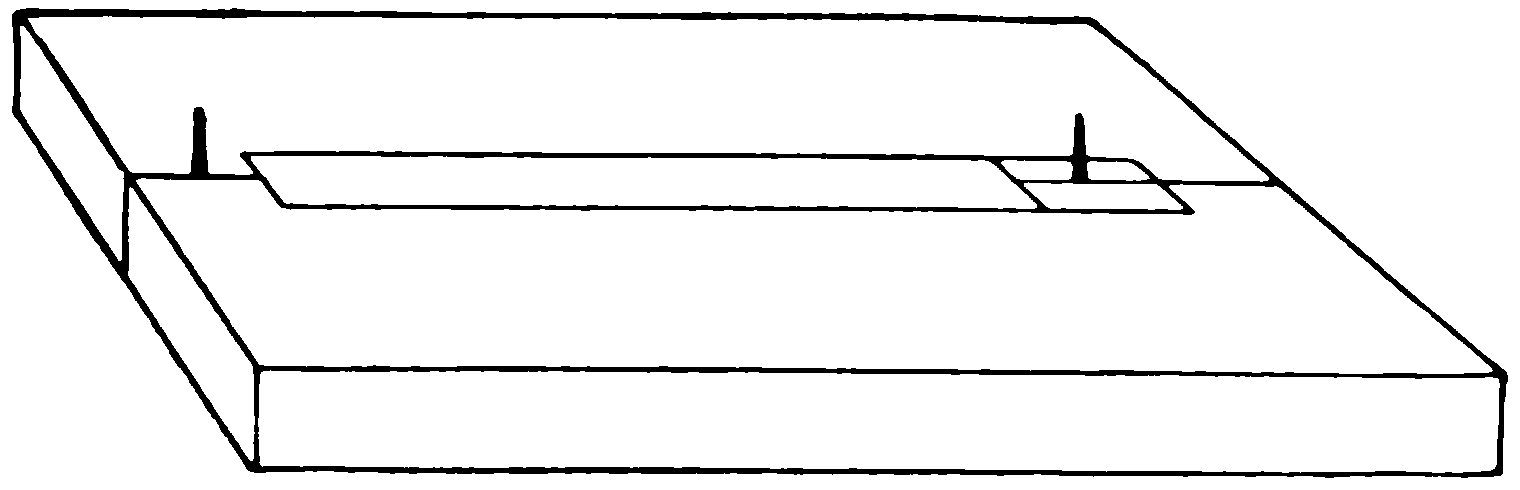
\includegraphics[width=0.62\linewidth]{pdf263-ellipse-describer.png}
\end{center}
\scanfooter

\scanpage{0264}{第37章、印刷頁250}
単位とする。糸を強く張ると、毛筆は第一の針の前方 $0\dd5$ 単位の位置を取り、糸の形は部分的に重なる二本の線となる。ここが曲線を描き始める点である。次に糸を張ったまま自然に進むように毛筆を回すと、糸は常に三角形の二辺をなす。短径に達すると三角形は二等辺三角形になる。このように糸を決して緩めずに描けば、楕円の自然な形が得られる。」

Aida はこの器具をどこから学んだかについて何も述べない。しかし弟子 Ichino Mokyō は一八二〇年の写本 \emph{Dayen-shū Tsūjutsu} に、楕円を描く器具が曲線に関する若干の理論とともに外国からもたらされたと書いている。われわれが述べた楕円描画器は、確実なことは何もわからないものの、Ichino のいう器具であったに違いない。\footnote{Hazama Jufū が製作した楕円描画器は Aida のものより興味深く、別の箇所で若干述べる。私は本書成立後にその器具を知った。}

3. ここでは Aida が楕円の焦点性質について研究した事柄を若干見る。同時代または後世の著作には、同様の考察法がほとんど見られないからである。

$a,b,c,k$ をそれぞれ長径、短径、焦点距離、糸の長さ\footnote{もちろん糸の両端は一本の針に固定され、他の針のまわりを通る。}とする。このとき $a-c$ は一方の針から長径端までの長さの二倍である。これに $2c$ を加えると $k=a+c$ を得る。また
\[
\left(\frac{k-c}{2}\right)^2-\left\{\left(\frac c2\right)^2+\left(\frac b2\right)^2\right\}=0
\qquad\text{または}\qquad a^2-b^2-c^3=0,
\]
であり、これによって $a,b$ から $c$ を決定する。図で矢 $AD=s$ が与えられ、弦 $PP'=h$ を求めるものとする。このとき
\[
PF_2^2=(a-PF_1)^2=(F_1D+F_1F_2)^2+PD^2,
\]
したがって
\[
a^2-2a\dd PF_1-ac+2sc=0,
\qquad\text{または}\qquad (a^2-ac+2sc)^2-(2a\dd PF_1)^2=0,
\]

\begin{center}
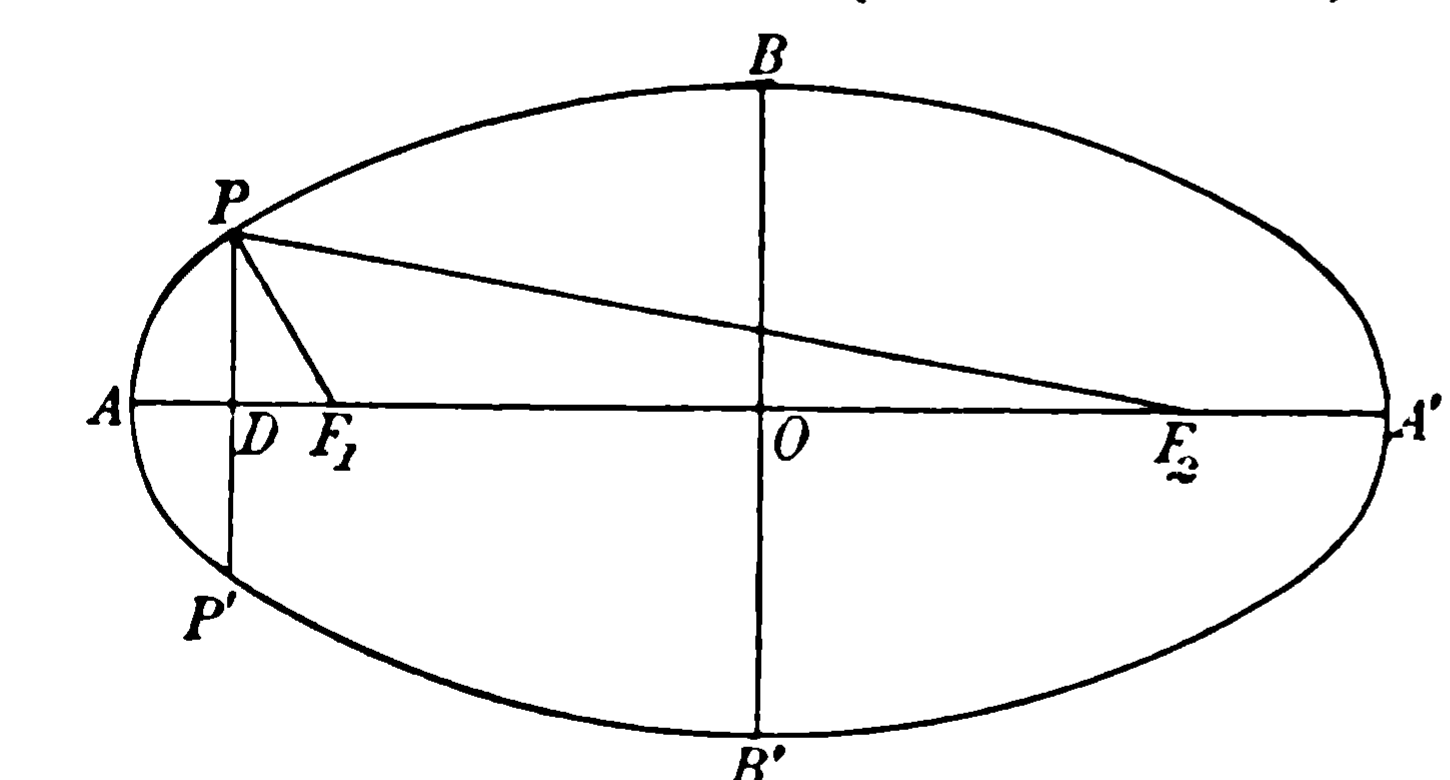
\includegraphics[width=0.55\linewidth]{pdf264-ellipse-focal-chord.png}
\end{center}
\scanfooter

\scanpage{0265}{第37章、印刷頁251}
しかし
\[
PF_1^2=PD^2+F_1D^2=PD^2+\left(\frac a2-\frac c2-s\right)^2,
\]
\[
\therefore\quad b^2as-b^2s^2-a^2PD^2=0,
\qquad\text{または}\qquad h=2\dd PD=2\sqrt{\frac{asb^2-s^2b^2}{a^2}}.
\]
したがって楕円弦 $h$ は、直径 $a$ の円の対応する弦に $b/a$ を掛けて得られる。ゆえに楕円弓または楕円全体の面積は、対応する円の面積に $b/a$ を掛けて得られる。原文のこの箇所には \emph{theréfere} とある。Aida はこの点についてさらに一つの証明法を試みる。短径に平行な弦を等間隔 $l$ ごとに $c_r$ とする。すると $c_r$ は $\frac ba\times c'_r$ と表され、$c'_r$ は直径 $a$ の円の対応する弦である。円弓の面積は
\[
\lim_{l=0}\sum\left\{\frac12(c'_r+c'_{r+1})l\right\},
\]
楕円弓の面積は
\[
\begin{aligned}
\lim_{l=0}\sum\frac{c_r+c_{r+1}}2\times l
&=\lim\sum\frac12\left(c'_r\frac ba+c'_{r+1}\frac ba\right)\times l\\
&=\frac ba\lim\sum\left(\frac{c'_r+c'_{r+1}}2\right)\times l,
\end{aligned}
\]
すなわち円弓の $b/a$ 倍である。楕円全体の面積についても明らかに同じである。

4. 短径の端を斜めに通って切られる弓形の場合、その弦を $c$、弦端点の縦座標と横座標を $h,k$ とし、長径を直径とする円の対応する縦座標を $h'$ とする。ここでこれらの長さは長径および短径まで測る。楕円に内接する長方形の長さと幅の間には
\[
a^2b^2-(\text{length})^2b^2-(\text{breadth})^2a^2=0
\]
が成り立つ。長方形の二辺をそれぞれ $2h,2k$ とし、式
\[
k^2=c^2-\left(\frac bc-h\right)^2
\]
を参照すれば、
\[
a^2b^2-4c^2b^2+4h^2b^2-4hb^3+b^4-4a^2h^2=0
\]
を得る。これにより $a,b,c$ から $h$ を決定できる。
\scanfooter

\scanpage{0266}{第37章、印刷頁252}
さらに
\[
h'=h\times\frac ab\qquad\text{および}\qquad c'^2=k^2+\left(\frac12a-h'\right)^2,
\]
ここで $c'$ は $c$ に対応する円の弦である。したがって弦 $c'$ をもつ円弓の面積を求めることができ、Aida はそれ以上の考察なしに、楕円弓は円弓の $b/a$ 倍であると結論する。

弓形の弦を長径の端から引く場合にも同じ結果を得る。

5. Aida の楕円弧長計算法は、他の日本数学者が用いたものと異なる原理に基づく点で興味深い。まず Aida は、長径端と短径端を結ぶ弦によって囲まれる弓形面積を、四分楕円弧長の第一近似とみなせると主張する。長径半分の中点に縦線を引けば、そこで分けられた二弧とその弦で囲まれる二つの弓形面積の和が第二近似を与える。次に長径半分を四等分し、分点に縦線を引く。この縦線で分けられた四弧と各弦で囲まれる四つの弓形面積を加え、その和を第三近似とする。このように進めれば逐次近似が得られる。分割数が数万に達すると、弓形面積は非常に薄くなり、実際には弓形の弧長を表すとみなせる。こうして最終的に四分楕円弧の長さに到達する。

Aida は明示的にこのように論じるが、実際の計算ではこの規則に正確には従わないようである。彼はさらに、楕円の逐次弦の式を求めると、それらは長径を直径とする円の対応する長さに比例しないと述べる。したがって楕円周長は円周に比例して求められないと結論し、次のように計算する。$t=a/2n$ と書けば、分点において長径まで測った補助円（原文 \emph{auxiliarly circle}）の縦座標は
\[
p_1'^2=(a-t)t,
\qquad p_2'^2=(a-2t)2t,
\qquad p_3'^2=(a-3t)3t,\ldots;
\]
\scanfooter

\scanpage{0267}{第37章、印刷頁253}
ここで $m=b/a$ と書くと、楕円の対応する縦座標は $p_1=p'_1m$, $p_2=p'_2m$, $p_3=p'_3m,\ldots$ であり、楕円弧の逐次弦は
\[
c_1^2=t^2+p_1^2,
\qquad c_2^2=t^2+(p_2-p_1)^2,
\qquad c_3^2=t^2+(p_3-p_2)^2,\ldots
\]
となる。Aida はこの考察をこれ以上進めない。彼は楕円周長の値を便利な形で表す最終式を持たなかったのであろう。その完成は後継者たちに残された。同じ主題に関する Sakabe, Kawai, Ichino, Tani, Shiraishi, Wada らの研究については、いつか詳細を述べられることを望む。

6. 著作第20巻で Aida は、四つの等しい円が楕円に外接し、その中心が長方形をなすときに成立する関係を求める。このため彼は添付の二図を描く。第一図では円 $B$ が四つの等円のうち二つに接する。接点 $C$ から長径へ垂線 $CK$ を下ろす。長径と短径を $a,b$、長方形の辺を $h,k$ とし、前者 $h$ は $b$ に平行とする。円 $A,B$ の直径も同じ文字で表す。$M$ を $h$ と $a$ の交点とする。第二図には対角線が $a$、一辺が $b$ の長方形を描く。$O'$ を中心とし、対角線上に $O'B'=OB$ を取る。$B'P$ をそれに直角に引き、$O'$ を通って一辺に平行な線まで延ばし、$PK'$ を別の辺に平行に引く。$K'$ は円 $A,B$ が楕円に接する点であると記される。

\begin{center}
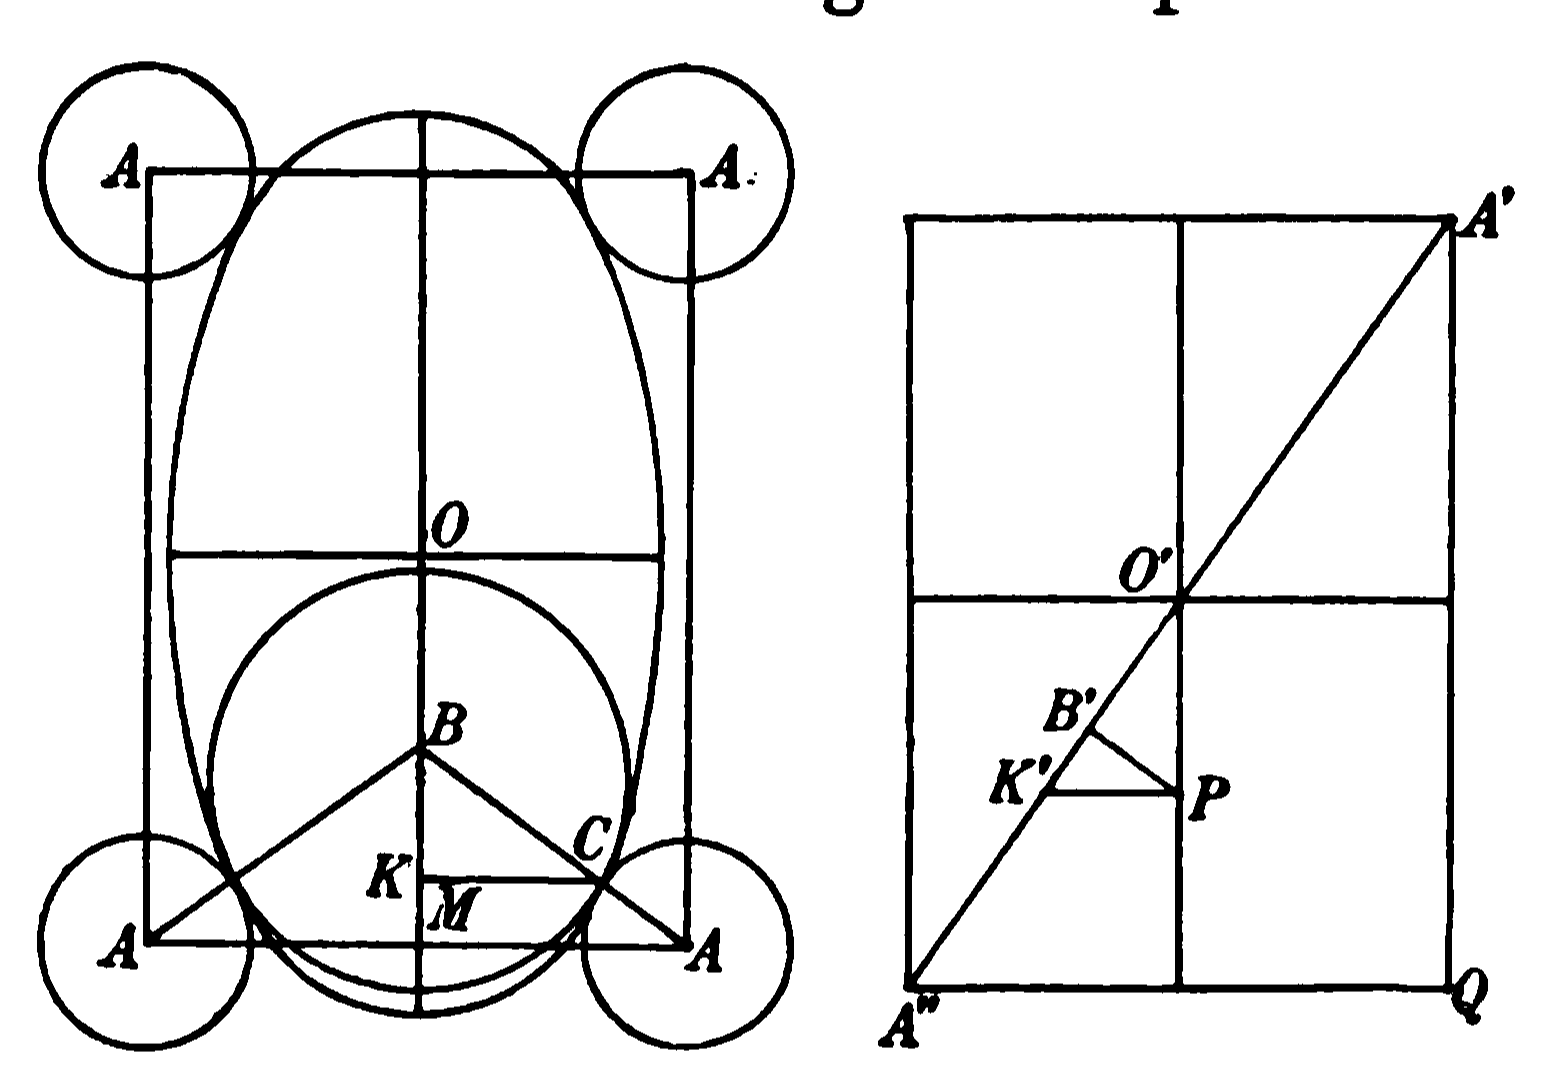
\includegraphics[width=0.76\linewidth]{pdf267-external-circles-projection-pair.png}
\end{center}

著者は説明なしに次の関係を与える。
\[
\alpha^2=A'Q^2=a^2-b^2,
\qquad \beta^2=B'P^2=\frac{b^2-B^2}{4},
\qquad \gamma=OB=O'B'=\frac{\beta\alpha}{4},
\]
\[
\delta=BK=B'K'=\frac{\beta b}{\alpha},
\qquad \varepsilon=BM=\frac k2-\gamma.
\]
したがって
\[
\frac B2:\frac{A+B}{2}=\delta:\varepsilon,
\qquad\text{または}\qquad \gamma B+\delta(A+B)=\frac{Bk}{2},
\]
\scanfooter

\scanpage{0268}{第37章、印刷頁254}
これを平方し、書き直すと
\[
\beta^2\alpha^4B^2+2\beta^2\alpha^2b^2(A+B)B+\beta^2b^4(A+B)^2-\frac14k^2B^2\alpha^2b^2=0,
\]
すなわち
\[
\tag{1}(\alpha^2B+b^2A^2)\beta^2-\frac14k^2B^2\alpha^2b^2=0.
\]
また $\xi^2=CK^2=\frac14B^2-\delta^2$ と書けば、
\[
\xi:\frac h2=\frac B2:\frac{A+B}{2},
\qquad\text{または}\qquad \xi^2(A+B)^2-\frac14B^2h^2=0,
\]
したがって
\[
\tag{2}(A+B)^2a^2B^2-(A+B)^2b^4-h^2\alpha^2B^2=0.
\]
関係 (1), (2) から
\[
\begin{aligned}
b^6A^2+(2b^4a^2A)B+(b^2a^4-b^4A^2-k^2b^2\alpha^2)B^2\\
{}-(2b^2a^2A)B^3-a^4B^4=0,
\end{aligned}
\]
\[
-b^4A^2-(2b^4A)B-(b^4-a^2A^2+h^2\alpha^2)B^2+(2a^2A)B^3+a^2B^4=0
\]
を得る。$B$ を消去すると求める関係は
\[
P^2Q^2+4Q^3a^2b^2A^2+4P^3+18PQa^2b^2A^2-27a^4b^4A^4=0
\]
となる。ここで $P,Q$ は
\[
-a^2A^2-b^2A^2-a^2b^2+h^2a^2+k^2b^2,
\qquad -a^2-b^2-A^2+h^2+k^2
\]
を表す。

7. 同じ問題をさらに別の方法で考える。この方法では一種の射影が用いられ、非常に興味深いが、私はその構成を十分には理解できない。著者自身の言葉を、可能な限り逐語的に訳して引用する（原文には \emph{auther's} とある）。「この問題は、添付図からわかるように、球に接する円柱を、その球が切断面の楕円周に接する点を通る平面で切ることによって生じると考えられる。こうして断面平面には楕円に接する円 $A$ が生じる。したがって問題のデータとして与えられた五量にもう一量を加え、全部で六量を考え、球の直径について二つの式を作る。それらの式を交乗して、求める関係に到達する。」\footnote{ここでは図を省略する。}\footnote{ここで Aida は、Seki Kōwa が行列式の処理で用いたのと同じ \emph{shajō}、すなわち交乗という語を用いる。計算の詳細は示されていないが、Aida は Seki と同じ理論を適用したのであろう。}
\scanfooter

\scanpage{0269}{第37章、印刷頁255}
いま述べた二式を作るため、ここに示す図が描かれる。球の直径を $S$ とし、
\[
\alpha^2=a^2-b^2,
\qquad \beta^2=\frac{S^2-A^2}{4},
\qquad \gamma=\frac{\beta a}{\alpha},
\]
\[
\delta^2=\frac{S^2}{4}-\gamma^2,
\qquad \varepsilon=\frac{\beta b}{\alpha},
\qquad \zeta=\frac k2-\varepsilon,
\qquad \Phi=\frac{\zeta b}{a}
\]
と書く。このとき
\[
\frac h2:\delta=\frac{S+b}{2}:\frac S2,
\]
すなわち
\[
(S+b)^2\delta^2-\frac{S^2h^2}{4}=0,
\]
または (1)
\[
(S+b)^2S^2\alpha^2-(S+b)^2S^2a^2+(S+b)^2A^2a^2-h^2S^2\alpha^2=0.
\]
さらに
\[
\Phi:\gamma=\frac b2:\frac S2,
\qquad\text{または}\qquad \Phi S-\gamma b=0,
\]
したがって
\[
\tag{2}\frac{k^2S^2\alpha^2}{4}-\beta^2(bS+a^2)^2=0.
\]

\begin{center}
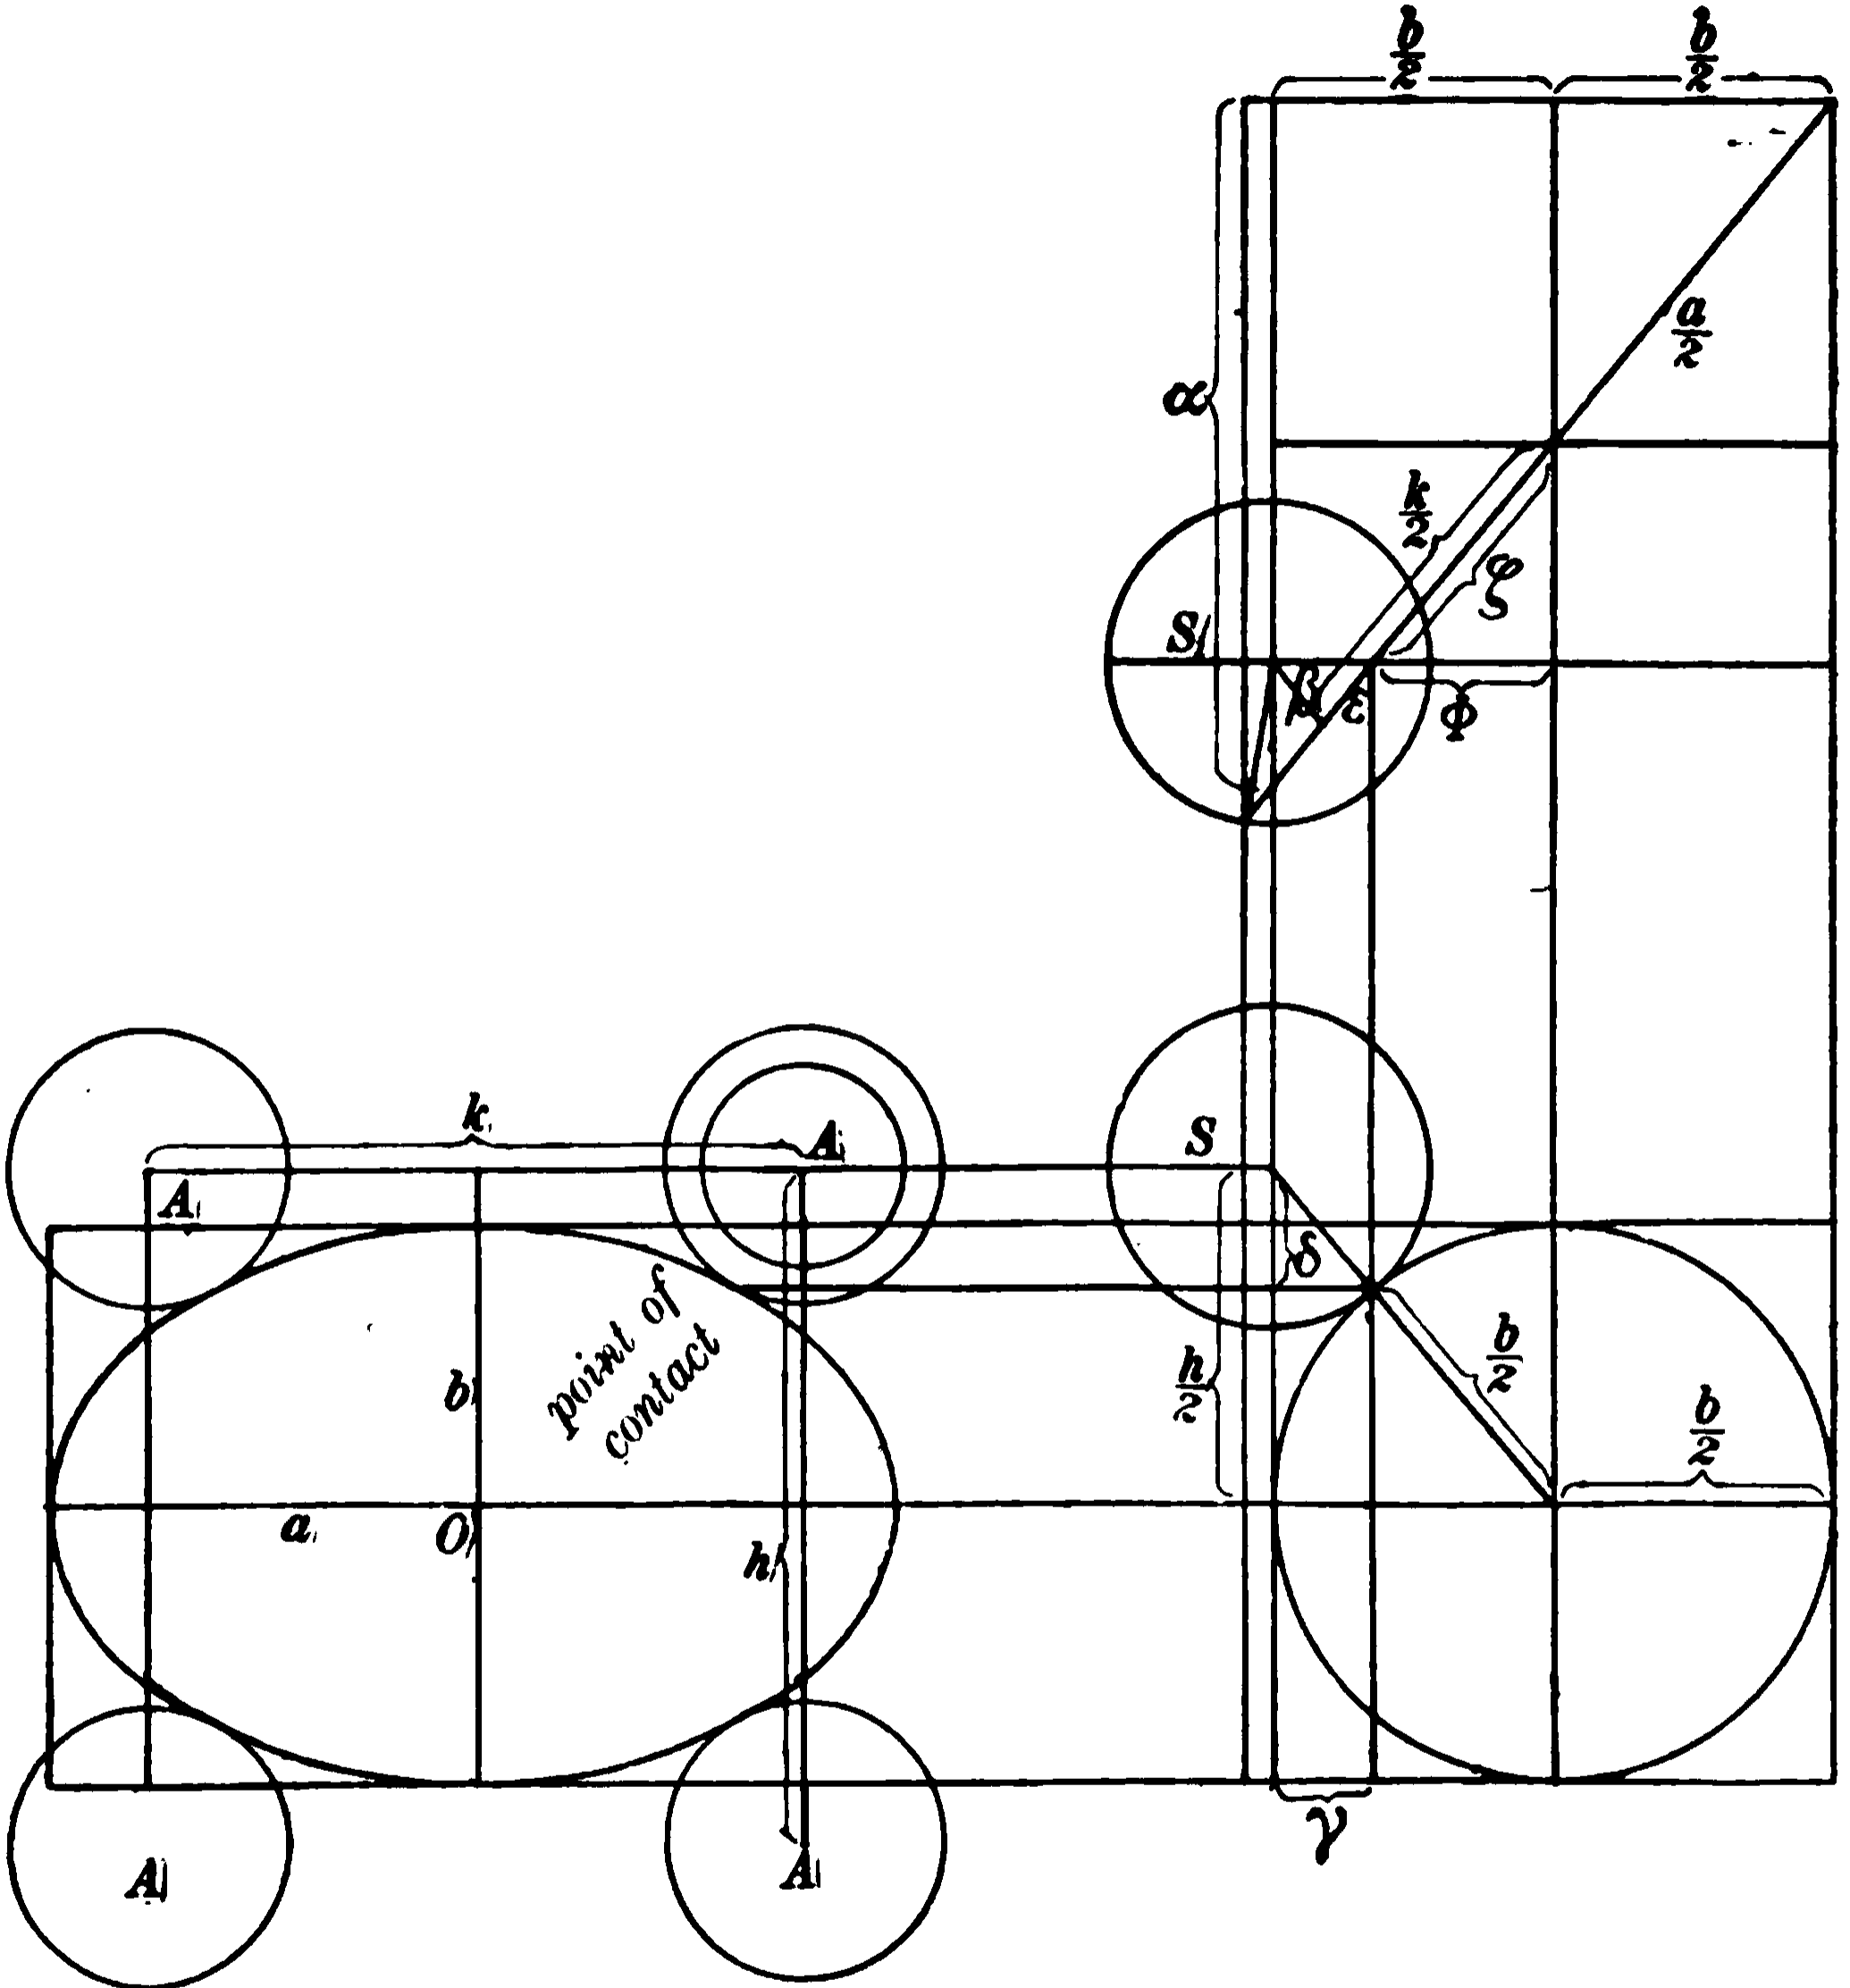
\includegraphics[width=0.82\linewidth]{pdf269-sphere-cylinder-projection.png}
\end{center}

この二関係から
\[
b^2a^2A^2+(2a^2A^2b)S+(a^2A^2-b^4-h^2\alpha^2)S^2-(2b^3)S^3-b^2S^4=0,
\]
\[
A^2a^4+(2A^2ba^2)S+(A^2b^2-a^4+k^2\alpha^2)S^2-(2a^2b)S^3-b^2S^4=0
\]
を得る。ここで $S$ を交乗によって消去すれば、先に得たのと同じ関係が得られる。

したがって著者は、試みた二つの手続から同じ公式が導かれ、得られた結果の正当性が示される、と付け加える。

8. Aida はさらに、中心から引いた楕円の動径を角の各一分ごとに求める問題を考える。この問題を解くため、動径の端を通って長径および短径に平行に引いた弦は
\scanfooter


\scanpage{0270}{印刷頁 256}
求められる。これらを $c_r$ および $p_r$ で表す。そうすれば、求める長さは次の式によって表されることが分かるであろう。
\[
-a^2b^2+(a^2c_r^2+b^2p_r^2)\,\varrho_r=0.
\]

この写本には、ほかにも注目に値するさまざまな点があるが、ここではそれらを詳しく論じることはしない。冗長に陥るおそれがあるからである。

\begin{center}
第38章。\\[1mm]
SHIRAISHI の楕円体表面の計算。
\end{center}
\phantomsection\addcontentsline{toc}{subsection}{第38章　SHIRAISHI の楕円体表面の計算}

旧日本の数学者の著作の中に回転楕円体の研究は稀ではなかったが、楕円体についての彼らの研究の成果にわれわれが出会うことは、それほど多くない。しかし、この主題に関する文書もいくつかあり、その顕著な一例が、一八二六年に刊行された Shiraishi Chōchū の \emph{Shamei Sampu} 第二巻中の一問題に見られる。この問題は楕円体の表面積を求めることに関するものである。この書物では結果のみが与えられ、解析は記されていない。$a$, $b$, $c$ を三つの主直径とし、次の量を作る。
\[
S=\left(1-\frac{c^2}{a^2}\right)\left(1-\frac{c^2}{b^2}\right),\quad N=1-\frac{1}{2}\left(\frac{c^2}{a^2}+\frac{c^2}{b^2}\right).
\]
このとき $ab\pi$ を原項と呼び、これを $D_0$ で表す。$\frac{1}{1\cdot 3}D_0N$ が第一差 $D_1$ である。第二、第三、\dots\ の差 $D_2, D_3, \dots$ は次のようにして作られる。
\begin{gather*}
D_2=\frac{1\cdot 3}{2\cdot 5}\left\{D_1N-\frac{1}{3^2}D_0S\right\},\quad D_3=\frac{3\cdot 5}{3\cdot 7}\left\{D_2N-\frac{1\cdot 2}{5^2}D_1S\right\},\\
D_4=\frac{5\cdot 7}{4\cdot 9}\left\{D_3N-\frac{3\cdot 3}{7^2}D_2S\right\},\quad D_5=\frac{7\cdot 9}{5\cdot 11}\left\{D_4N-\frac{5\cdot 4}{9^2}D_3S\right\},\dots,
\end{gather*}
そして原項 $D_0$ を相次ぐ差だけ減じたものが、楕円体の表面積の公式を与える。

この公式は \emph{Shamei Sampu} において著者の門人 Ikeda Tei-ichi の名で与えられているが、彼が著者であるというのは名目上のことにすぎないようである。というのは、一八二四年第六月一三日付の、彼の師の書いた写本が残っているからである。旧日本では、師の成果がその門人の名で刊行されることが時々あった。実際、さまざまな刊行物にこのような例がおびただしく見られる。

\scanpage{0271}{印刷頁 257}
以下では、この問題に対する Shiraishi の取扱いを述べなければならない。\footnote{本文中に与えられている諸式は、種々の原因によってあまり正確でないかもしれないが、われわれの記述は、著者の従った方法の本質を示すのに十分であろう。}

楕円体の表面積を求めるために、Shiraishi はここに示すような図を作る。
\begin{center}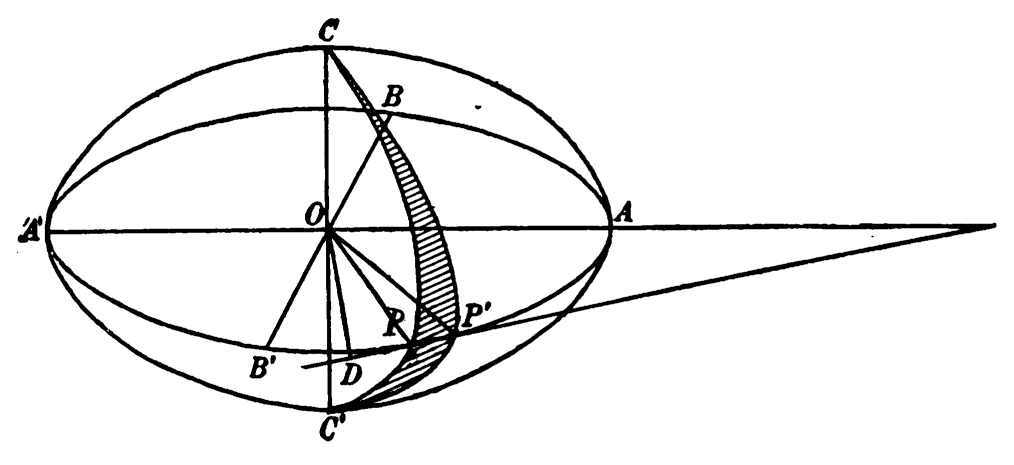
\includegraphics[width=0.6\linewidth]{pdf271-a.png}\end{center}
$AA'=a$ が、これに垂直な平面によって $2n$ 等分されるとする。これらの平面のうち相続く二平面が、$AA'=a$ と $BB'=b$ を含む平面による楕円体の切り口と、点 $P$ および $P'$ で交わるとする。このとき $2.PP'=s_r$ をその切り口の弧の要素に取れば、
\[
s_r^2=\frac{1}{l}\left\{k^2-\frac{Bk^4r^2}{a^2}\right\},
\]
を得る。ここで
\[
k=\frac{a}{n},\quad l=1-\frac{k^2r^2}{a^2},\quad B=1-\frac{b^2}{a^2}.
\]
$p_r$ で中心 $O$ から直線 $PP'$ に下ろした垂線 $OD$ を表せば、$p_r=kb/s_r\sqrt{l}$ である。

これらの関係は説明なしに与えられており、別の写本で説明されているものとして述べられているが、ここではこれらの事柄には関わらないことにする。

さて Shiraishi は、軸 $CC'=c$ を通り、かつそれぞれ点 $P$ および $P'$ を通る二平面によって切り取られる楕円体面の帯を考える。このような帯は図中で斜線を施した部分によって示されており、これを面積の要素すなわち $S_r$ とする。そして Shiraishi は次の公式を与える。
\[
S_r=2s_rp_r\left(1-\frac{C}{1\cdot3}-\frac{C^2}{3\cdot5}-\frac{C^3}{5\cdot7}-\frac{C^4}{7\cdot9}-\cdots\right),
\]
ここで $1-\frac{c^2{s_r}^2l}{b^2k^2}$ の代りに $C$ と書いた。Shiraishi は、われわれの手元にある写本ではこの公式の構成を説明しておらず、ただ図によって、それが、面積の要素を対応する部分によって与えられるものと仮定することから得られたことを示すのみである

\scanpage{0272}{印刷頁 258}
\noindent 楕円柱のものであり、その楕円柱は $c$ と $2p_r$ を主直径とする楕円を底とし、直径 $c$ を通って引いた二平面によって切られ、この二平面はその中央部において母線から長さ $s_r$ を切り取る。

$A=1-c^2/b^2$ と書けば、量 $C$ は次のように書くことができる。
\[
C=1-\frac{c^2s_r{}^2l}{k^2b^2}=A+\frac{Bc^2k^2r^2}{a^2b^2}.
\]

こうして $S_r$ の式は次のようになる。
\[
\begin{array}{r@{}l@{}l@{}l@{}l@{}l@{}l}
=\dfrac{b}{\sqrt{l}}\Biggl\{\qquad k\biggl( & 1 & {}-\dfrac{A}{1\cdot 3} & {}-\dfrac{A^2}{3\cdot 5} & {}-\dfrac{A^3}{5\cdot 7} & {}-\dfrac{A^4}{7\cdot 9} & {}-\cdots\biggr)\\[2mm]
{}+\dfrac{Bc^2k^3r^2}{b^2a^2}\biggl( & & {}-\dfrac{1}{1\cdot 3} & {}-\dfrac{2A}{3\cdot 5} & {}-\dfrac{3A^2}{5\cdot 7} & {}-\dfrac{4A^3}{7\cdot 9} & {}-\cdots\biggr)\\[2mm]
{}+\dfrac{B^2c^4k^5r^4}{b^4a^4}\biggl( & & & {}-\dfrac{1}{3\cdot 5} & {}-\dfrac{3A}{5\cdot 7} & {}-\dfrac{6A^2}{7\cdot 9} & {}-\cdots\biggr)\\[2mm]
{}+\dfrac{B^3c^6k^7r^6}{b^6a^6}\biggl( & & & & {}-\dfrac{1}{5\cdot 7} & {}-\dfrac{4A}{7\cdot 9} & {}-\cdots\biggr)\\[2mm]
{}+\dfrac{B^4c^8k^9r^8}{b^8a^8}\biggl( & & & & & {}-\dfrac{1}{7\cdot 9} & {}-\cdots\biggr)\\[2mm]
\multicolumn{7}{l}{\quad{}+\cdot\;\;\cdot\;\;\cdot\;\;\cdot\;\;\cdot\;\;\cdot\;\;\cdot\;\;\cdot\;\;\cdot\;\;\cdot\;\;\cdot\;\;\cdot\;\;\cdot\;\;\cdot\;\;\cdot\;\Biggr\}.}
\end{array}
\]

総和を行って極限に移れば（これは表を用いて行うことができる）、楕円体の表面は $=$ $ab\pi$ と次の式との積として得られるであろう。
\[
\begin{array}{r@{}l@{}l@{}l@{}l@{}l@{}l}
\biggl( & 1 & {}-\dfrac{A}{1\cdot 3} & {}-\dfrac{A^2}{3\cdot 5} & {}-\dfrac{A^3}{5\cdot 7} & {}-\dfrac{A^4}{7\cdot 9} & {}-\cdots\biggr)\\[2mm]
{}+\dfrac{Bc^2}{2b^2}\biggl( & & {}-\dfrac{1}{1\cdot 3} & {}-\dfrac{2A}{3\cdot 5} & {}-\dfrac{3A^2}{5\cdot 7} & {}-\dfrac{4A^3}{7\cdot 9} & {}-\cdots\biggr)\\[2mm]
{}+\dfrac{3B^2c^4}{8b^4}\biggl( & & & {}-\dfrac{1}{3\cdot 5} & {}-\dfrac{3A}{5\cdot 7} & {}-\dfrac{6A^2}{7\cdot 9} & {}-\cdots\biggr)\\[2mm]
{}+\dfrac{15B^3c^6}{348b^6}\biggl( & & & & {}-\dfrac{1}{5\cdot 7} & {}-\dfrac{4A}{7.9} & {}-\cdots\biggr)\\[2mm]
{}+\dfrac{105B^4c^8}{384b^8}\biggl( & & & & & {}-\dfrac{1}{7\cdot 9} & {}-\cdots\biggr)+\cdots
\end{array}
\]

この式を変形するために、Shiraishi は $\varrho=Bc^2/b^2$ と書き、さらに次のように書く。
\[
A_1=A+\tfrac{1\varrho}{2},\quad A_2=A+\tfrac{3\varrho}{4},\quad A_3=A+\tfrac{5\varrho}{6},\quad A_4=A+\tfrac{7\varrho}{8},\;\cdot\;\cdot\;;
\]

\scanpage{0273}{印刷頁 259}
ついで次のように書き、
\[
\begin{aligned}
&1 = D_0',\\
&A + \frac{\varrho}{2} = 1\,.\,3\,D_1' = B_1,\\
&A^2 + \frac{2A\varrho}{2} + \frac{3\varrho^2}{8} = 3\,.\,5D_2' = B_2,\\
&A^3 + \frac{3A^2\varrho}{2} + \frac{3\cdot 3A\varrho^2}{8} + \frac{5\varrho^3}{48} = 5\,.\,7\,D_3' = B_3,\\
&A^4 + \frac{4A^3\varrho}{2} + \frac{3\cdot 6A^2\varrho^2}{8} + \frac{5\cdot 15A\varrho^3}{48} + \frac{105\varrho^4}{384} = 7\,.\,9\,D_4' = B_4, \ldots;
\end{aligned}
\]
次の諸量を作り、
\[
\begin{aligned}
&\qquad B_1 = D_0' A_1 = C_1,\\
&\frac{2}{1}(B_1 A_2 - B_2) = \frac{A\varrho}{2} = C_2,\\
&\frac{3}{2}(B_2 A_3 - B_3) = \frac{A^2\varrho}{2} + \frac{A\varrho}{8} = C_3,\\
&\frac{4}{3}(B_3 A_4 - B_4) = \frac{A^3\varrho}{2} + \frac{2A^2\varrho^2}{8} + \frac{3A\varrho^3}{48}\unclear{3 or 8} = C_4,\\
&\frac{5}{4}(B_4 A_5 - B_5) = \frac{A^4\varrho}{2} + \frac{3A^3\varrho^2}{8} + \frac{3\cdot 3A^2\varrho^3}{48} + \frac{15A\varrho^4}{384} = C_5, \ldots,
\end{aligned}
\]
また次の諸量をも作る。
\[
\begin{aligned}
&1\cdot 2(- B_1 A_2 + B_2) + B_1 A = A^2 = (1),\\
&\frac{3\cdot 3}{2}\,(- B_2 A_3 + B_3) + B_2 A = A^3 - \frac{A^2\varrho}{2} = (2),\\
&\frac{5\cdot 4}{3}\,(- B_3 A_4 + B_4) + B_3 A = A^4 - \frac{2A^3\varrho}{2} - \frac{A^2\varrho^2}{8} = (3),\\
&\frac{7\cdot 5}{4}\,(- B_4 A_5 + B_5) + B_4 A = A^5 - \frac{3A^4\varrho}{2} - \frac{3A^3\varrho^2}{8} - \frac{3A^2\varrho^3}{48},\unclear{comma or speck} = (4), \ldots
\end{aligned}
\]

最後の二組から次を得る。
\[
\begin{aligned}
&2\cdot 2(- B_1 A_2 + B_2) + B_1 A = A^2 - \frac{A\varrho}{2},\\
&\frac{3\cdot 4}{2}(- B_2 B_3 + B_3) + B_2 A = A^3 - \frac{2A^2\varrho}{2} - \frac{6A\varrho^2}{8},\\
&\frac{4\,.\,6}{3}(- B_3 A_4 + B_4) + B_3 A = A^4 - \frac{3A^3\varrho}{2} - \frac{3A^2\varrho^2}{8} - \frac{3A\varrho^3}{48},\\
&\frac{5\cdot 8}{8}(- B_4 A_5 + B_5) + B_4 A = A^5 - \frac{4A^4\varrho}{2} - \frac{6A^3\varrho^2}{8} - \frac{4\cdot 3A^2\varrho^3}{48}\\
&\hspace{18em} - \frac{15A\varrho^4}{384}, \ldots;
\end{aligned}
\]
これらはそれぞれ $\frac{(2)}{A}$, $\frac{(3)}{A}$, $\frac{(4)}{A}$, $\cdots$ に等しい。したがってこれら二組を等置すれば、いくつかの簡単な変形の後に次を得る。

\scanpage{0274}{印刷頁 260 (top left)}
\[
\begin{array}{@{}l@{}c@{}l@{}}
\phantom{1\cdot 3^2}tD_0' & & {}=1\cdot 3\,D_1',\\[1mm]
1\cdot 3^2tD_1'-{} & ApD_0' & {}=2\cdot 3\cdot 5\,D_2',\\[1mm]
\frac{3\cdot 5^2\,\mathrm{t}}{2}D_2' & {}-1\cdot 3\,ApD_1' & {}=\frac{3\cdot 5\cdot 7}{2}D_3',\\[1mm]
\frac{5\cdot 7^2t}{3}D_3' & {}-3\cdot 5\,ApD_2' & {}=\frac{4\cdot 7\cdot 9}{3}D_4',\\[1mm]
\frac{7\cdot 9^2t}{4}D_4' & {}-5\cdot 7\,ApD_3' & {}=\frac{7\cdot 9\cdot 11}{4}D_5',\ldots,
\end{array}
\]
ここで $t=A+\frac{1}{2}\varrho$ および $p=A+\varrho$ と書く。これらから、$D_0'=1$ を $D_0=abx$ で置き換え、$D'_1$, $D_2'$, \ldots\ を $D_1$, $D_2$, \ldots で置き換え、用いた文字にいくらかの変更を加えると、一八二六年の \emph{Shamei Sampu} から再現したものとしてわれわれが与えた公式がただちに得られる。

\emph{注意。} 同じ問題に Tani Shōmo がその著 \emph{Tetsujutsu Shin-i} 第二巻で取り組んでいるのが見られる。Tani の手続きは Shiraishi のとった手続きとは異なる。彼は楕円体を、直径 $a$ に垂直に等間隔で引いた平行平面によって分割し、こうして得られる面積の要素を楕円錐台の側面とみなす。彼の最終結果は Shiraishi によって得られたものと同じである。

一八四四年の Hasegawa Kō の \emph{Sampō Kyūseki Tsūkō} は、おそらく同じ問題の解析が印刷された最初の刊行物であった。

われわれが述べた解析と、それによって得られた結果とは、正確であるか否かがあまり確かではないけれども、それでも歴史的見地からは興味あるものとわれわれは信ずる。

\begin{center}
第39章。\\[1mm]
SAKABE-KAWAI の方程式の解法。
\end{center}
\phantomsection\addcontentsline{toc}{subsection}{第39章　SAKABE-KAWAI の方程式の解法}

1. Sakabe Kōhan は一八〇三年に写本 \emph{Rippō Eijiku}、すなわち「交互に増減する値による三次方程式の根の近似」を書いた。最初に同様の展開を研究し、Sakabe を促してわれわれの前にある写本を書かせたのは、Fujita Seishin であった。前者は自分の解法を得ると、後者のもとへ行ってこの件についての意見を求めた。Fujita のもとの解法は、立方根の開法と三乗することとを繰り返し適用して行われていたので、Sakabe は平方根の開法と平方することとを繰り返し用いることによって改良を試みた。これに対して Fujita は少なからず不快に思い、自分自身の考案の正当性を主張した。「方程式は三次の

\scanpage{0275}{印刷頁 261}
次であるならば」と Fujita はいうのであった。「それを解くには当然開立法を採用すべきであり、さもなければその方法は正統なものとは見なしえない。」それゆえ Sakabe は、Fujita の目的にかなう方法を考案した。

2. Sakabe は、一般形の三次方程式は \emph{soroban} によって解けるように取り扱うことはできないと主張する。そこで彼はまず、これを二次の項が欠けるような形に変換する。たとえば
\[ -a_0 + a_1x - a_2x^2 + a_3x^3 = 0 \]
を三次方程式の一つの形とする。このとき $x = x_1/3a_3$ と書けば、方程式は次のようになる。
\[ -27a_0a_3^2 + 9a_1a_3x_1 - 3a_2x_1^2 + x_1^3 = 0. \]
さらに $x_1 = 3a_2 + x_2$ と書けば、次を得る。
\[ (-27a_0a_3^2 + 9a_1a_2a_3 - 7a_2^3) + (9a_1a_3 - 3a_2^2)\,x_2 + x_2^3 = 0, \]
ここでは二次の項が消えている。したがって、絶対項と一次の項の符号に応じて、次の三つの形を考えなければならない。
\[ -a + bx + x^3 = 0, \quad a + bx - x^3 = 0, \quad a - bx + x^3 = 0, \]
これらを (\emph{A})、(\emph{B}) および (\emph{C}) と呼ぶ。これらの方程式の根の一つは正である。もちろん正根が存在しない場合も起こりうるが、そのときにはいずれかの項の符号を変えることによって、根の符号を正にすることができる。ゆえに、上の三つの形を考えれば十分である。

3. 方程式 (\emph{A}) は $a = bx + x^3$ と書くことができ、したがって $a > x^3$ である。それゆえ第一近似として $X_1^3 = a$ を取る。$X_1$ は明らかに $> x$ である。次に $x^3 = a - bx$ であるから、第二近似としては $X_2^3 = a - bX_1$ を取ることになる。$X_2$ は $< x$ である。このようにして、さらに先の近似として次のものを取ることができる。
\[ X_3^2 = a - bX_2, \quad X_4^2 = a - bX_3, \quad X_5^2 = a - bX_4, \ \ldots . \]
これによって $X_1$、$X_2$、$X_3$、\ldots{} は、$x$ の実際の値より交互に大きく、また小さくなる。こうして (\emph{A}) の正根は、次の無限式に展開されたことになる。
\[ x = \ldots (a - (a - (a - a^{\frac{1}{3}}b)^{\frac{1}{3}}b)^{\frac{1}{3}}b)^{\frac{1}{3}} \ldots . \]

方程式 (C) は二つの正根をもち、そのうち大きい方の $x_1$ は次のように近似される。
\[ X_1^3 = -a, \quad X_2^3 = -a + X_1b, \quad X_3^3 = -a + X_2b, \ \ldots, \]

\scanpage{0276}{印刷頁 262 (top left)}
そのうち $X_1$ は、もちろん近似値を表すものとみなしてはならない。小さいほうの根を得るには、すでに得た大きいほうの根 $x_1$ をもって、開方の演算（算木で行われるもの、すなわち天元術によるもの）を実行しなければならない。こうして
\[
(a - bx_1 + x_1^3) + (-b + x_1^2)\,x + x_1x^2 + x^3 = 0,
\]
を得る。あるいは因数 $x$ を除くと
\[
(-b + x_1^2) + x_1x + x^2 = 0,
\]
となり、これから第二の根 $x_2$ の値が得られる。ゆえに
\[
x_2 = -\frac{x_1}{2} + \sqrt{b - \frac{3x_1^2}{4}}.
\]

方程式 $(B)$ においては次のようになる。
\[
X_1^3 = a, \quad X_2^3 = a + X_1b, \quad X_3^3 = a + X_2b, \;\ldots\,.
\]

これらの近似について Sakabe は、実用上不便であり、また収束が遅いので、決して十分に満足すべきものではないと述べている。

4. 次に、Sakabe が実用的価値をもつと考える解法を示す。方程式 $(A)$ を $\frac{a}{b} = x + \frac{x^3}{b}$ の形に書いて、$X_1 = a/b$ と置く。これは明らかに $x$ の実際の値より大きい。次に方程式を $x = a/(b + x^2)$ の形に書いて、
\[
X_2 = \frac{a}{b + X_1^2}, \quad X_3 = \frac{a}{b + X_2^2}, \;\ldots
\]
を逐次近似値とする。これらの量は $x$ の実際の値より交互に大きく、また小さく、次第にそれに近づく。

たとえば方程式 $-8 + 5x + x^3 = 0$ では、実際に計算すれば、$X_{13}$ が最初の二桁まで正しいことがわかるであろう。このように収束は非常に遅く、それゆえ Sakabe は別の解法を考案した。それは前者から次のようにして導かれる。
\[
\begin{array}{l|l|l|}
X_1 = \frac{a}{b} & \;X_2 = \frac{X_1 + Y_1}{2} & \;X_3 = \frac{X_2 + Y_2}{2} \\[3mm]
Y_1 = \frac{a}{b + X_1^2} & \;Y_2 = \frac{a}{b + X_2^2} & \;Y_3 = \frac{a}{b + X_3^2}
\end{array}
\quad \ldots,
\]
と書けば、$X_1$, $X_2$, \ldots\ が逐次近似値である。

5. 方程式 $(B)$ は $a = x^3 - bx = x\,(x^2 - b)$ と書くことができ、これから $b$ が $< x^2$ であることがわかる。ゆえに $X_1^2 = b$ は小さめの近似値である。次に方程式を $x^2 = b + a/x$ の形に書いて、次のように取る。
\[
X_2^2 = b + \frac{a}{X_1}, \quad X_3^2 = b + \frac{a}{X_2}, \quad X_4^2 = b + \frac{a}{X_3}, \;\ldots
\]

\scanpage{0277}{印刷頁 263}
\noindent を逐次近似値として取る。これらは増加と減少を交互に繰り返す。

6. 方程式 $(C)$ を $a = bx - x^3 = x\,(b - x^2)$ と書けば、明らかに $b > x^2$ である。そこで第一近似値として $X_1 = b^{\frac{1}{2}}$ を取る。これは必ず実際の値より大きい。次に方程式を $x^2 = b - a/x$ の形に書いて、$X_2^2 = b - \frac{a}{X_1}$, $X_3^2 = b - \frac{a}{X_2}$, $\cdots$ を逐次近似値として取る。これらは一段ごとに値が増していく。この根は二つの正根のうち大きい方である。

これらの根の第二のものを得るには、$\frac{a}{b} = x - \frac{x^3}{b}$ と書く。第一近似値 $X_1 = a/b$ は明らかに $x$ の実際の値より小さい。次に方程式を $x = a/(b - x^2)$ の形に書き直して、逐次近似値を
\[
X_2 = \frac{a}{b - X_1^2}, \qquad X_3 = \frac{a}{b - X_2^2}, \qquad X_4 = \frac{a}{b - X_3^2}, \ \cdots,
\]
とする。これらはすべて実際の根より小さい。

7. Fujita Seishin が得て Sakabe に示した公式については、われわれは何も知らない。しかし後に彼はその結果を Yedo の Atago 寺に掲げた。その写しが \emph{Rippō Sanka-Jutsu Kigen} と題して残っている。彼がその解法を掲げたのは一八二〇年のことであった。その中で彼は、これらの結果を二〇年前に得たと述べている。そこでは、彼は近似値 $X_1^3 = a + b$ および $X_r^3 = a + bX_{r-1}$ を用いて方程式 $x^3 = a + bx$ を解いている。その導出はきわめて明白である。$a$ または $b$ が負である場合には、$X$ の式においてこれらの量を負にするだけでよい。

方程式が二つの正根をもつ場合には、Fujita はそれらの根のうち第二のものを求める規則を与えている。

方程式 $x^3 \pm (bx - a) = 0$ の場合には、Fujita はまた近似値 $X_1 = a/b$, $X_r = a/(b \pm X_{r-1}^2)$ を用いている。これは Sakabe の解法の一つと同じである。Sakabe がその写本に書いているところから判断してよいならば、これは Fujita が相手から学んだもののように思われる。

8. Sakabe が \emph{Rippō Eijiku} を書いたのと同じ年、すなわち一八〇一年に、その門人 Kawai Kyūtoku は、二巻からなる \emph{Kaishiki Shimpō}、すなわち「方程式を解く新しい方法」を出版した。そこに盛り込まれた方法は、通常 Sakabe の創案であると信じられている。これは日本の数学者たちの著作の中でも最も重要なものの一つである。

いま方程式を次の形に書くとする。
\[
a_1 + a_2 x + a_3 x^2 + \cdots + a_n x^{n-1} + a_{n+1} x^n = 0,
\]

\scanpage{0278}{印刷頁 264 (top left)}
ここで係数は正または負の数である。この方程式は一般に $n$ 個の根をもち、著者はそれらを第一根、第二根、\dots、第 $n$ 根と呼ぶ。そして著者は証明なしに、これらの根は $a_{n+1}$, $a_n$; $a_n$, $a_{n-1}$; \dots; $a_2$, $a_1$ がそれぞれ異符号であるか同符号であるかに従って、正または負になると主張する。

第 $r$ 根を求めるために、著者は量 $B = -P/Q$ を作る。ここで
\begin{gather*}
P = \frac{a_1 + a_2 A + \ldots + a_{n-r+1} A^{n-r}}{A^{n-r}},\\
Q = a_{n-r+2} + a_{n-r+3} A + \cdots + a_{n+1} A^{r-1}.
\end{gather*}
その際、$A$ にはどんな値を用いてもよいが、ただ $P$ と $Q$ がそれぞれ $a_{n-r+1}$ および $a_{n-r+2}$ と異なる符号をとるように選ばなければならない。次に、やはり任意に、ただし前と同じ制限のもとで別の量 $A'$ を取り、$B$ と同じ仕方で $B'$ を作る。$A - B$ と $A' - B'$ が異符号であれば、方程式は一般に $A$ と $A'$ の間にある根をもつ。この定理は、書物の内容のすべてと同じく、説明なしに与えられている。

この定理を利用すれば、$A$ にさまざまな値を取って試みることにより、第 $r$ 根がその間にある限界を一歩一歩狭めることができる。このようにして第一近似値 $X_1$ を定めることができる。しかし、ときには $A$, $A'$, $B$, $B'$ の平均を $X_1$ として取ってもよい。ごく粗い値でも目的に適うからである。$A$ から $B$ を得たときと同じようにして $X_1$ から $X_2$ を作れば、この $X_2$ が第二近似値である。この手続きを繰り返せば、逐次の近似値が得られる。著者は何の推論も試みていないが、この方法は Sakabe がその \emph{Rippō Eijiku} において従ったのと同じ仕方で考案されたものと思われる。

上の解法は次のように述べることができる。代数方程式を（$f_r$ は $r$ 次であるとして）次の形に書く。
\[ f_r(x) + x^{r+1} f_s(x) = 0 \quad\text{または}\quad x = -f_r(x)/x^r f_s(x) = \Phi(x). \]
$x_1$ を方程式をほぼ満たす $x$ の値とすれば、量 $x_2 = \Phi(x_1)$, $x_3 = \Phi(x_2)$, \dots\ が逐次の近似値として取られる。すなわち、$\Phi^i(x) = \Phi\{\Phi^{i-1}(x)\}$ と書けば、量 $x = \lim_{i=\infty} \Phi^i(x_1)$ は一般に方程式の根である。もちろん $x_1$ の値については、上に述べたような制限が必要である。

9. 例によって、これらの特殊な工夫が実際にどのように用いられたかを示そう。方程式
\[ 630 + 2711x + 2562x^2 + 194x^3 - 318x^4 - 25x^5 + 6x^6 = 0 \]
の第一根は正である。最高次の二項の符号が異なるからである。この根については $A = 10$, $B = 8{\cdot}6$; $A' = 9$, $B' = 9$ となる。このように $A'$ と $B'$ が等しいので、この等しい値が根の値である。第二根は

\scanpage{0279}{印刷頁 265}
\noindent 負であって、$-5$ に等しい。$A = -5$ が同じ値の $B$ を与えるからである。第三根はほぼ $3{\cdot}5$ に等しい。というのは、次を得るからである。
\[
A_1 = 8,\ B = 4{\cdot}16;\quad A_2 = 4,\ B_2 = 3{\cdot}14;\quad A_3 = 3,\ B_3 = 4{\cdot}04.
\]
第四根および第五根は、それぞれ $-2$ および $-1$ である。第六根については $A = -0{\cdot}5$, $B = -0{\cdot}41$ および $A' = -0{\cdot}3$, $B' = -0\;31$\unclear{$-0{\cdot}31$; decimal point not visible} を得る。これから、この根は $-0{\cdot}5$ と $-0{\cdot}3$ の間にあると推論される。この場合、$A$ と $B$ の差はきわめて小さいので、それらの平均 $\frac{1}{2}\,(A' + B') = -0{\cdot}31$ を第一近似値として取ってよい。

10. 次の方程式の第二根に対しては
\[
1\,74720 - 9392x + 168x^2 - x^3 = 0,
\]
$A$ の値として 50, 40, 30, 20, 10 を取る。すると、対応する $B$ の値は $49{\cdot}9$, $39{\cdot}2$, $25{\cdot}8$, $4{\cdot}43$、および負であることが見出されるであろう。これらはすべて役に立たない。したがって当然、目的に適うためには、より大きな $A$ の値を探さなければならない。こうして次を得る。
\[
\begin{array}{l|l|l}
\begin{array}{@{}l@{}} A_1 = 55\\ B_1 = 55{\cdot}002 \end{array} &
\begin{array}{@{}l@{}} A_2 = 58\\ B_2 = 57{\cdot}99 \end{array} &
\therefore\ \frac{A_1 + A_2 + B_1 + B_2}{4} = 56{\cdot}19,
\end{array}
\]
したがって、56 を第一近似値として取ることになる。

11. $-3 + 11x - x^2 + x^3 = 0$ の第一根については、次を得る。
\begin{center}
\begin{tabular}{c|c|c|c|c|c|c}
$A$ & 1 & 10 & 20 & 30 & $0{\cdot}2$ & 0 3\unclear{0·3; decimal point not visible}\\
\hline
$B$ & 負 & 負 & $0{\cdot}45$ & $0{\cdot}63$ & 21 & 負
\end{tabular}
\end{center}
\noindent $A$ の増加とともに $A$ と $B$ の差が増加するならば、根は一般に 1 より小さいであろう。しかしここでは、$A$ の値が小さいときに $B$ が負となる。このことは、実根が存在しないことを示している。というのは、最高次の二項の符号が異なっているので、いまの場合、根は正でなければならないからである。この場合は \emph{mushō}、すなわち字義通りには「根なし」\footnote{\emph{mushō} すなわち「根なし」は、Seki が用いた用語であった。彼はこの語を、正の実根も負の実根ももたない方程式を示すのに用いた。}と称され、これによって根が虚であることが意味される。しかしながら、虚数が日本の数学者に知られていたとは思われない。

第二根は負であろう。しかし $A = 0{\cdot}1$, $0{\cdot}8$, 2 に対応する $B$ の値は負、36、負であるから、これもまた「根なし」の場合である。

$A$ と $B$ の差が常にきわめて大きいか、あるいは常に負の結果に導くならば、対応する根は虚、すなわち「根なし」であろう。

\scanpage{0280}{印刷頁 266}
12. $343 - 196x + 35x^2 - 2x^3 = 0$ の第一根、第二根、第三根は、それぞれ 7、7 および 3·5 である。第一根の場合には、$A$ と $B$ の値は次の通りである。
\begin{center}
\begin{tabular}{c|c|c|c|c|c|c|c}
$A$ & 10 & 9 & 8 & 6 & 5 & 4 & 3 \\
\hline
$B$ & 9·4 & 8·7 & 7·9 & 5·9 & 4·76 & 3·71 & 3·88
\end{tabular}
\end{center}

この例から分かるように、$A$ と $B$ の差は初めは大きく、次第に減少し、それから再び増大する。ここで $A$ と $B$ の第六および第七の値については、量 $A_6 - B_6$ と $A_7 - B_7$ とが異なる符号をもつ。しかし、この関係が存在するのは、$A$ と $B$ の差が小さい位置においてではなく、差がかなり増大したところにおいてである。この事実は、考察中の根に等しいか、またはほぼ等しい別の根が存在するであろうことを示している。したがって、まず副次的な一根または数根を調べなければならない。第二根については次のようになる。
\begin{center}
\begin{tabular}{c|c|c|c|c|c|c|c}
$A$ & 3 & 4 & 5 & 6 & 8 & 9 & 10 \\
\hline
$B$ & 2·816 & 4·08 & 5·096 & 6·036 & 8·059 & 9·28 & 10·78
\end{tabular}
\end{center}
ここでも第一根の場合と同じ事情が生ずる。ゆえに、第一根と第二根とは等しいか、またはほぼ等しいであろうと結論する。この種の根は、$A$ と $B$ の差が最も小さいところにある。したがって第一根と第二根は、ともに 6 と 8 の間にあるであろう。$A_1$ が $B_1$ を超える一方で $A_2$ が $B_2$ より小さいという事実は、値 3·5 をもつ第三根の存在に起因する。

13. Sakabe-Kawai の方法におけるもう一つの重要な点は、Seki が円弧および円周の測定において用いたものに類似した処理を適用して行う、得られた結果の補正あるいは数値的補間であろう。

方程式
\[
4732 - 2860x + 179x^2 + 40x^3 - 3x^4 = 0
\]
の第一根に対する逐次近似値が次の通りであるとする。
\[
r_1 = 12,\ r_2 = 12{\cdot}598,\ r_3 = 12{\cdot}851,\ r_4 = 12{\cdot}946.
\]
補正のために、著者は次のように取る。
\[
r_4' = \frac{r_4 m - r_3}{m - 1} = 13{\cdot}001, \quad \text{ただし } m = \frac{r_4 - r_3}{r_3 - r_2} = 2{\cdot}7.
\]
次に、第五近似値 $r_5$ を通常の仕方で計算し、これを次の式によって補正する。
\[
r_5' = \frac{r_5 m - r_4'}{m - 1} = 12{\cdot}99996\ 6,
\]

\scanpage{0281}{印刷頁 267}
\noindent ここで $m$ は前と同じである。そして同様に進めると、
\[
r_6' = 13{\cdot}00000\;1, \quad r_7' = 12{\cdot}99999\;996, \ \ldots .
\]
に至る。

第三根についても同様に、
\[
\begin{gathered}
r_1 = 8, \quad r_2 = 7{\cdot}3892, \quad r_3 = 7{\cdot}1423, \quad r_4 = 7{\cdot}0509, \quad m = 2{\cdot}7,\\
r_4' = 6{\cdot}997, \quad r_5' = 7{\cdot}00007, \quad r_6' = 6{\cdot}99999\;8, \quad r_7' = 7{\cdot}00000\;004, \ldots
\end{gathered}
\]
を得る。

14. 方程式 $-936 + 373x + 8x^2 - 5x^3 = 0$ の第一根では、最初の四つの近似値は $r_1 = 7{\cdot}2$, $r_2 = 8{\cdot}35$, $r_3 = 7{\cdot}8492$, $r_4 = 8{\cdot}0656$ である。そしてこの場合、$r_4$ の修正値は次のようになる。
\[
r_4' = \frac{r_4 m + r_3}{m + 1} = 8{\cdot}00002, \quad \text{ここで } m = \frac{r_2 - r_3}{r_4 - r_3} = 2{\cdot}3.
\]
それから $r_5$ を計算すると、次のようになる。
\[
\begin{gathered}
r_5' = \frac{r_5 m + r_4'}{m + 1} = 8{\cdot}00000\;0006,\\
r_6' = 8{\cdot}00000\;00000\;01, \quad x_7' = 8{\cdot}00000\;00000\;00005,
\end{gathered}
\]
以下同様である。この修正の仕方は前節で試みたものと同じであるが、ただ諸項の符号が考慮に入れられている点だけが異なる。

負である第二根については、
\[
r_1 = 8{\cdot}0448, \quad r_2 = 10{\cdot}147, \quad r_3 = 7{\cdot}9310, \quad r_4 = 10{\cdot}317, \ \ldots,
\]
を得る。ただし符号は無視してある。これらの値は、ある極限に近づく傾向をもたず、反対に次第に発散することを示している。したがって、われわれの通常の方法はこのような場合には適用できない。しかし補間の手続きによって、その結果は利用できるものとなる。ここで $m$ の値は $= 0{\cdot}9$ であり、修正された逐次近似値は次のように得られる。
\[
\begin{aligned}
&r_4' = 9{\cdot}05, \quad r_5' = 9{\cdot}001, \quad r_6' = 9{\cdot}00002,\\
&r_7' = 9{\cdot}00000\;03, \quad r_8' = 9{\cdot}00000\;0007, \ \ldots .
\end{aligned}
\]

15. 代数方程式に二つ以上の根が存在することを、日本人は一七世紀の中頃から知っていた。そして Seki Kōwa は、一般に $n$ 次方程式には $n$ 個の根が存在することさえ知っていた。しかし、方程式のすべての実根を常に求めることのできる方法については、一八世紀あるいはそれ以前の諸世紀の著作には何も見られない。しかし Sakabe-Kawai の業績が、必ずしもそのような方法の最初の例であったわけではない。Kawai 自身が一例を引用しているのは、\emph{Sampō Shōjo}\footnote{\emph{Sampō Shōjo} は Settsu 国の一医師によって書かれた。この医師は後に Yedo に住んだ。この書はその娘 Taira Aki-ko によって編集され、出版された。}、すなわち「乙女の

\scanpage{0282}{印刷頁 268}
\noindent 算術」であり、これは一八六八年の維新以前に日本で女性の手によって編集された唯一の数学書である。引用文は次の通りである。

「方程式
\[
\begin{aligned}
&40216\ 08000 - 19081\ 02200x + 3611\ 34200x^2\\
&{}- 340\ 70206x^3 + 16\ 01620x^4 - 30000x^5 = 0
\end{aligned}
\]
にはいくつの根が存在するか、またそれらの値はいくらか。

「答。\quad $x_1 = 10$,\quad $x_2 = 13\,\frac{1}{3}$,\quad $x_3 = 10\frac{1}{250}$,\quad $x_4 = 10\frac{1}{20}$。

「これは Nakai という人が提出した問題である。彼が誰から数学を学んだのかは、私にはわからない。しかしこの問題についていえば、これは非常に興味深いものである。何年か前に Ōsaka にいたとき、Sugawara 公の廟でこの問題を知り、私は非常に長いあいだこれについて考え込んでいたが、ついにある考えが心に浮かんだ。もしこれを解くことのできる超人的な者がいるならば、その結果は疑いなく注目に値し、まったく新しいものであろう、と私は考えたのである。しかしながら、ついに私は幸運にも答を得ることができた。私の用いた方法は注意深く秘密に保たれてきており、私はそれ以来、あえてそれを誰にも示したことがない。それゆえ、この書においても私は解法を説明せず、ただ根の値を与えるだけである。」

「乙女の算術」は一七七四年に印刷された。

Kawai はその書の中で、ここに引用した方程式には 10 に等しいもう一つの根があり、それはすでに求められた根の一つと同じであると付け加えている。彼の時代以前に、等根が二つとして数えられていたとは思われない。

\begin{center}
第40章。\\[1mm]
\emph{YENRI} 計算に用いられるいくつかの表、および無限次の方程式。
\end{center}
\phantomsection\addcontentsline{toc}{subsection}{第40章　YENRI 計算に用いられるいくつかの表、および無限次の方程式}

後の日本の数学者たちの \emph{yenri} の方法は、直径、弦などのようなある量を $n$ 個の等しい部分に分け、これらの等しい部分の一つに関係するある量を、計算すべき大きさの要素として求め、分割された量のすべての部分について総和を行い、それから極限 $n = \infty$ に移ることにあった。これらの段階を常にすべて経るのは非常に煩わしかったので、日本の数学者たちは、特別に作られた表によってこれらの演算を行うことを工夫した。この表は \emph{jō-hyō}、すなわち文字通りには「畳む表」と呼ばれた。積分の演算は、日本では動詞 \emph{tatamu}、すなわち「畳む」あるいは「畳むこと」によって呼ばれた。\emph{Jō} はこの語を表す文字である。したがって、これらの表は積分の目的のために用いられる表を意味するものとされていた。

\scanpage{0283}{印刷頁 269}
最初の表は Wada Nei（一七八七---一八四〇）によって計算されたと普通信じられている。しかし、この点についてわれわれは確かではない。Aida Ammei によって与えられた表もある。

Wada の扱い方に従って、表の構成の一端を述べる。彼によれば、\emph{yenri} 算法に適用される極限の値を求めるには三つの基本的な場合があり、それらは次の式によって表される。
\begin{align*}
&\lim\nolimits_{n=\infty}\,(1^k+2^k+3^k+\cdots+n^k)\times\frac{1}{n^{k+1}},\\
\text{および}\qquad\qquad&\lim\nolimits_{n=\infty}\,\{1^k+2^k+3^k+\cdots+(n\mp k)^k\}\times\frac{1}{n^{k+1}},
\end{align*}
ここで $k$ は任意の整数であり、また $t$ はいかに大きくても有限な数である。

数列 $1^k+2^k+3^k+\cdots+n^k$ の和と、この和に $1/n^{k+1}$ を掛けた積とは、$k=0, 1, 2, 3, \ldots$ に対して、それぞれ次の値をもつ。
\[
\begin{array}{l@{\hspace{6em}}|@{\hspace{4em}}l}
\frac{n}{1}, & \frac{1}{1},\\[3mm]
\frac{n^2}{2}+\frac{n}{2}, & \frac{1}{2}+\frac{1}{2}\,\frac{1}{n},\\[3mm]
\frac{n^3}{3}+\frac{n^2}{2}+\frac{n}{6}, & \frac{1}{3}+\frac{1}{2}\,\frac{1}{n}+\frac{1}{6}\,\frac{1}{n^2},\\[3mm]
\frac{n^4}{4}+\frac{n^3}{2}+\frac{n^2}{4}, & \frac{1}{4}+\frac{1}{2}\,\frac{1}{n}+\frac{1}{4}\,\frac{1}{n^2},\\[3mm]
\frac{n^5}{5}+\frac{n^4}{2}+\frac{n^3}{3}-\frac{n}{3},\ \cdots & \frac{1}{5}+\frac{1}{2}\,\frac{1}{n}+\frac{1}{3}\,\frac{1}{n^2}-\frac{1}{3}\,\frac{1}{n^3},\ \cdots
\end{array}
\]
いま極限 $n=\infty$ に移ると、$n^{-1}$ およびその冪を掛けた項はすべて消え、$k=0, 1, 2, 3, \ldots$ に対して
\[
\lim\nolimits_{n=\infty}\frac{1}{n^{k+1}}\,(1^k+2^k+3^k+\cdots+n^k)=\frac{1}{1},\ \frac{1}{2},\ \frac{1}{3},\ \cdots
\]
を得る。

加え合わせる項の数が $n\mp t$ である場合には、$n$ 項の公式において $n$ の代りに $n\mp t$ を代入し、その結果に $1/n^{k+1}$ を掛けて極限に移る。そうすれば、すでに得たのと同じ値を得る。

\emph{tō}、\emph{sai}、\emph{nan}、\emph{hoku}（東、西、南、北）と呼ばれる Wada の\unclear{Wada's / Wada's.}表は、非常によく知られている。もし
\[
E=1-\frac{r}{n},\quad W=1+\frac{r}{n},\quad S=1-\frac{r^2}{n^2},\quad N=1+\frac{r^2}{n^2},
\]
と書けば、これらの表はこれらの量に関する折り畳みの結果である。これらの表では、最上行と最左列とに示された量の積を積分した結果が、これらの因数と同じ列および同じ行に位置する欄に与えられている。

\scanpage{0284}{印刷頁 270 (top left)}
\begin{center}
\renewcommand{\arraystretch}{2.2}\setlength{\tabcolsep}{4pt}
\begin{tabular}{|c||c|c|c|c|c|c|c|c|}
\hline
$\diagdown$ & $1$ & $E$ & $E^2$ & $E^3$ & $E^4$ & $E^5$ & $E^6$ & \dots\\
\hline\hline
$\frac{1}{n}$ & $\frac{1}{1}$ & $\frac{1}{2}$ & $\frac{1}{3}$ & $\frac{1}{4}$ & $\frac{1}{5}$ & $\frac{1}{6}$ & $\frac{1}{7}$ & $\cdots$\\
\hline
$\frac{r}{n^2}$ & $\frac{1!}{1.2}$ & $\frac{1!}{2.3}$ & $\frac{1!}{3.4}$ & $\frac{1!}{4.5}$ & $\frac{1!}{5.6}$ & $\frac{1!}{6.7}$ & $\frac{1!}{7.8}$ & $\cdots$\\
\hline
$\frac{r^2}{n^3}$ & $\frac{2!}{1.2.3}$ & $\frac{2!}{2\;3.4}$ & $\frac{2!}{3.4.5}$ & $\frac{2!}{4.5.6}$ & $\frac{2!}{5.6.7}$ & $\frac{2!}{6.7.8}$ & $\frac{2!}{7.8.9}$ & $\cdots$\\
\hline
$\frac{r^3}{n^4}$ & $\frac{3!}{1.2.3.4}$ & $\frac{3!}{2.3.4.5}$ & $\frac{3!}{3.4.5.6}$ & $\frac{3!}{4.5.6.7}$ & $\frac{3!}{5.6.7.8}$ & $\frac{3!}{6.7.8.9}$ & $\frac{3!}{7.8.9.10}$ & $\cdots$\\
\hline
\dots & \dots & \dots & \dots & \dots & \dots & \dots & .\,. & \dots\\
\hline
\end{tabular}
\end{center}

\begin{center}
\renewcommand{\arraystretch}{2.2}\setlength{\tabcolsep}{4pt}
\begin{tabular}{|c||c|c|c|c|c|c|c|c|}
\hline
$\diagdown$ & $\sqrt{E}$ & $\sqrt{E}^{3}$ & $\sqrt{E}^{5}$ & $\sqrt{E}^{7}$ & $\sqrt{E}^{9}$ & $\sqrt{E}^{11}$ & $\sqrt{E}^{13}$ & .\,.\\
\hline\hline
$\frac{1}{n}$ & $\frac{1}{3}$ & $\frac{1}{5}$ & $\frac{1}{7}$ & $\frac{1}{9}$ & $\frac{1}{11}$ & $\frac{1}{13}$ & $\frac{1}{15}$ & $\cdots$\\
\hline
$\frac{r}{n^2}$ & $\frac{2}{3.5}$ & $\frac{2}{5.7}$ & $\frac{2}{7.9}$ & $\frac{2}{9.11}$ & $\frac{2}{11\;13}$ & $\frac{2}{13.15}$ & $\frac{2}{15.17}$ & $\cdots$\\
\hline
$\frac{r^2}{n^3}$ & $\frac{2.4}{3.5.7}$ & $\frac{2.4}{5.7.9}$ & $\frac{2.4}{7.9.11}$ & $\frac{2.4}{9.11.13}$ & $\frac{2.4}{11.13.15}$ & $\frac{2.4}{13.15.17}$ & $\frac{2.4}{15.17.19}$ & $\cdots$\\
\hline
$\frac{r^3}{n^4}$ & $\frac{2.4\;6}{3.5.7.9}$\unclear{2.4.6} & $\frac{2.4.6}{5.7.9.11}$ & $\frac{2.4.6}{7.9.11.13}$ & $\frac{2.4.6}{9.11.13.15}$ & $\frac{2.4.6}{11.13.15.17}$ & $\frac{2.4.6}{13.15.17.19}$ & $\frac{2.4.6}{15.17.19.21}$ & $\cdots$\\
\hline
\dots & \dots & \dots & \dots & \dots & \dots & \dots & \dots & .\,.\\
\hline
\end{tabular}
\end{center}

この表のすべての項には因数 2 を掛けなければならない。旧日本の人々が分数指数の記法をもたなかったことは注目に値する。

\begin{center}
\renewcommand{\arraystretch}{2.2}\setlength{\tabcolsep}{4pt}
\begin{tabular}{|c||c|c|c|c|c|c|c|c|}
\hline
$\diagdown$ & $1$ & $S$ & $S^2$ & $S^3$ & $S^4$ & $S^5$ & $S^6$ & \dots\\
\hline\hline
$\frac{1}{n}$ & $\frac{1}{1}$ & $\frac{2}{1.3}$ & $\frac{2.4}{1.3.5}$ & $\frac{2.4.6}{1.3.5\;7}$\unclear{1.3.5.7} & $\frac{2.4.6.8}{1.3.5.7.9}$ & $\frac{2.4.6.8.10}{1.3.5.7.9.11}$ & $\frac{2.4.6.8.10.12}{1.3.5.7.9.11.13}$ & $\cdots$\\
\hline
$\frac{r^2}{n^3}$ & $\frac{1}{3}$ & $\frac{2}{3.5}$ & $\frac{2.4}{3.5.7}$ & $\frac{2.4.6}{3.5.7.9}$ & $\frac{2.4.6\;8}{3.5.7.9.11}$\unclear{2.4.6.8} & $\frac{2.4.6.8.10}{3.5.7.9\;11.13}$ & $\frac{2.4.6.8.10.12}{3.5.7.9.11.13.15}$ & $\cdots$\\
\hline
$\frac{r^4}{n^5}$ & $\frac{1}{5}$ & $\frac{2}{5.7}$ & $\frac{2.4}{5.7.9}$ & $\frac{2.4.6}{5.7.9.11}$ & $\frac{2.4.6.8}{5\;7.9.11.13}$\unclear{5.7.9.11.13} & $\frac{2.4.6.8.10}{5.7.9.11.13.15}$ & $\frac{2.4.6.8.10.12}{5.7.9.11.13.15.17}$ & $\cdots$\\
\hline
$\frac{r^5}{n^7}$\unclear{$r^6$} & $\frac{1}{7}$ & $\frac{2}{7.9}$ & $\frac{2.4}{7.9.11}$ & $\frac{2.4.6}{7.9\;11.13}$\unclear{7.9.11.13} & $\frac{2.4.6.8}{7.9.11.13.15}$ & $\frac{2.4.6.8.10}{7.9.11.13.15.17}$ & $\frac{2.4.6\;8.10.12}{7.9.11.13.15.17.19}$\unclear{2.4.6.8.10.12} & $\cdots$\\
\hline
\dots & \dots & \dots & \dots & \dots & \dots & \dots & \dots & \dots\\
\hline
\end{tabular}
\end{center}

\scanpage{0285}{印刷頁 271}
\begin{center}
\renewcommand{\arraystretch}{1.8}
\begin{tabular}{|c||c|c|c|c|c|c|c|c|}
\hline
$\diagdown$ & $1$ & $S$ & $S^2$ & $S^3$ & $S^4$ & $S^5$ & $S^6$ & \dots \\
\hline\hline
$\frac{r}{n^2}$ & $\frac{1}{2}$ & $\frac{1}{4}$ & $\frac{1}{6}$ & $\frac{1}{8}$ & $\frac{1}{10}$ & $\frac{1}{12}$ & $\frac{1}{14}$ & \dots \\
\hline
$\frac{r^3}{n^4}$ & $\frac{2}{2.4}$ & $\frac{2}{4.6}$ & $\frac{2}{6.8}$ & $\frac{2}{8.10}$ & $\frac{2}{10.12}$ & $\frac{2}{12.14}$ & $\frac{2}{14.16}$ & \dots \\
\hline
$\frac{r^5}{n^6}$ & $\frac{2.4}{2.4.6}$ & $\frac{2.4}{4.6.8}$ & $\frac{2.4}{6.8.10}$ & $\frac{2.4}{8.10.12}$ & $\frac{2.4}{10.12.14}$ & $\frac{2.4}{12.14.16}$ & $\frac{2.4}{14.16.18}$ & \dots \\
\hline
$\frac{r^7}{n^8}$ & $\frac{2.4.6}{2.4.6.8}$ & $\frac{2.4.6}{4.6.8.10}$ & $\frac{2.4.6}{6.8.10.12}$ & $\frac{2.4.6}{8.10.12.14}$ & $\frac{2.4.6}{10.12.14.16}$ & $\frac{2.4.6}{12.14.16.18}$ & $\frac{2.4.6}{14.16.18.20}$ & \dots \\
\hline
\dots & \dots & \dots & \dots & \dots & \dots & \dots & \dots & \dots \\
\hline
\end{tabular}
\end{center}

\begin{center}
\renewcommand{\arraystretch}{1.8}
\begin{tabular}{|c||c|c|c|c|c|c|c|c|}
\hline
$\diagdown$ & $\sqrt{S}$ & $\sqrt{S}^{3}$ & $\sqrt{S}^{5}$ & $\sqrt{S}^{7}$ & $\sqrt{S}^{9}$ & $\sqrt{S}^{11}$ & $\sqrt{S}^{13}$ & \dots \\
\hline\hline
$\frac{1}{n}$ & $\frac{1}{2}$ & $\frac{1.3}{2.4}$ & $\frac{1.3.5}{2.4.6}$ & $\frac{1.3.5.7}{2.4.6.8}$ & $\frac{1.3\ldots 9}{2.4\ldots 10}$ & $\frac{1.3\ldots 11}{2.4\ldots 12}$ & $\frac{1.3\ldots 13}{2.4\ldots 14}$ & \dots \\
\hline
$\frac{r^2}{n^3}$ & $\frac{1}{2.4}$ & $\frac{1.3}{2.4.6}$ & $\frac{1.3.5}{2.4.6.8}$ & $\frac{1.3.5.7}{2.4.6.8.10}$ & $\frac{1.3\ldots 9}{2.4\ldots 12}$ & $\frac{1.3\ldots 11}{2.4\ldots 14}$ & $\frac{1.3\ldots 13}{2.4\ldots 16}$ & \dots \\
\hline
$\frac{r^4}{n^5}$ & $\frac{1}{2.4.6}$ & $\frac{1.3}{2.4.6.8}$ & $\frac{1.3.5}{2.4.6.8.10}$ & $\frac{1.3.5.7}{2.4.6\ldots 12}$ & $\frac{1.3\ldots 9}{2.4\ldots 14}$ & $\frac{1.3\ldots 11}{2.4\ldots 16}$ & $\frac{1.3\ldots 13}{2.4\ldots 18}$ & \dots \\
\hline
$\frac{r^6}{n^7}$ & $\frac{1}{2.4.6.8}$ & $\frac{1.3}{2.4.6.8.10}$ & $\frac{1.3.5}{2.4.6\ldots 12}$ & $\frac{1.3.5.7}{2.4.6\ldots 14}$ & $\frac{1.3\ldots 9}{2.4\ldots 16}$ & $\frac{1.3\ldots 11}{2.4\ldots 18}$ & $\frac{1.3\ldots 13}{2.4\ldots 20}$ & \dots \\
\hline
\dots & \dots & \dots & \dots & \dots & \dots & \dots & \dots & \dots \\
\hline
\end{tabular}
\end{center}

この表のすべての項には因数 $\frac{\pi}{2}$ を掛けなければならない。さらに、第二、第三、第四、\dots{} の横の行にある項には、それぞれ 1, 1.3, 1.3.5, 1.3.5.7, \dots{} を掛けなければならない。

\begin{center}
\renewcommand{\arraystretch}{1.8}
\begin{tabular}{|c||c|c|c|c|c|c|c|c|}
\hline
$\diagdown$ & $\sqrt{S}$ & $\sqrt{S}^{3}$ & $\sqrt{S}^{5}$ & $\sqrt{S}^{7}$ & $\sqrt{S}^{9}$ & $\sqrt{S}^{11}$ & $\sqrt{S}^{13}$ & \dots \\
\hline\hline
$\frac{r}{n^2}$ & $\frac{1}{3}$ & $\frac{1}{5}$ & $\frac{1}{7}$ & $\frac{1}{9}$ & $\frac{1}{11}$ & $\frac{1}{13}$ & $\frac{1}{15}$ & \dots \\
\hline
$\frac{r^3}{n^4}$ & $\frac{2}{3.5}$ & $\frac{2}{5.7}$ & $\frac{2}{7.9}$ & $\frac{2}{9.11}$ & $\frac{2}{11.13}$ & $\frac{2}{13.15}$ & $\frac{2}{15.17}$ & \dots \\
\hline
$\frac{r^5}{n^6}$ & $\frac{2.4}{3.5.7}$ & $\frac{2.4}{5.7.9}$ & $\frac{2.4}{7.9.11}$ & $\frac{2.4}{9.11.13}$ & $\frac{2.4}{11.13.15}$ & $\frac{2.4}{13.15.17}$ & $\frac{2.4}{15.17.19}$ & \dots \\
\hline
$\frac{r^7}{n^8}$ & $\frac{2.4.6}{3.5.7.9}$ & $\frac{2.4.6}{5.7.9.11}$ & $\frac{2.4.6}{7.9.11.13}$ & $\frac{2.4.6}{9.11.13.15}$ & $\frac{2.4.6}{11.13.15.17}$ & $\frac{2.4.6}{13.15.17.19}$ & $\frac{2.4.6}{15.17.19.21}$ & \dots \\
\hline
\dots & \dots & \dots & \dots & \dots & \dots & \dots & \dots & \dots \\
\hline
\end{tabular}
\end{center}

\scanpage{0286}{印刷頁 272}
\begin{center}
\setlength{\tabcolsep}{3pt}
\renewcommand{\arraystretch}{1.6}
\begin{tabular}{|c||c|c|c|c|c|c|c|c|}
\hline
 & $1$ & $E$ & $E^{2}$ & $E^{3}$ & $E^{4}$ & $E^{5}$ & $E^{6}$ & $\dots$ \\
\hline\hline
$\dfrac{1}{n}\times\dfrac{1}{\sqrt{\dfrac{r}{n}}}$ & $\dfrac{1}{1}$ & $\dfrac{2}{1.3}$ & $\dfrac{2.4}{1.3.5}$ & $\dfrac{2.4.6}{1.3\ 5.7}$ & $\dfrac{2.4.6.8}{1.3\ 5.7.9}$ & $\dfrac{2.4.6.8.10}{1.3.5.7\ 9.11}$ & $\dfrac{2.4.6\dots 12}{1.3.5.7.9.11.13}$ & $\dots$ \\
\hline
$\dfrac{1}{n}\times\sqrt{\dfrac{r}{n}}$ & $\dfrac{1}{3}$ & $\dfrac{2}{3.5}$ & $\dfrac{2.4}{3.5.7}$ & $\dfrac{2.4.6}{3.5.7.9}$ & $\dfrac{2.4.6.8}{3.5.7.9.11}$ & $\dfrac{2.4.6.8.10}{3.5.7.9.11.13}$ & $\dfrac{2.4.6\dots 12}{3.5.7\dots 13.15}$ & $\dots$ \\
\hline
$\dfrac{1}{n}\times\sqrt{\dfrac{r}{n}}^{3}$ & $\dfrac{1}{5}$ & $\dfrac{2}{5.7}$ & $\dfrac{2.4}{5.7.9}$ & $\dfrac{2.4.6}{5.7.9.11}$ & $\dfrac{2.4.6.8}{5.7.9.11.13}$ & $\dfrac{2.4.6.8.10}{5.7\ 9\dots 13.15}$ & $\dfrac{2.4.6\dots 12}{5.7.9\dots 15.17}$ & $\dots$ \\
\hline
$\dfrac{1}{n}\times\sqrt{\dfrac{r}{n}}^{5}$ & $\dfrac{1}{7}$ & $\dfrac{2}{7.9}$ & $\dfrac{2.4}{7.9.11}$ & $\dfrac{2.4.6}{7.9.11.13}$ & $\dfrac{2.4.6.8}{7.9.11.13.15}$ & $\dfrac{2.4.6.8\ 10}{7.9.11\dots 17}$ & $\dfrac{2.4.6\dots 12}{7.9.11\dots 17.19}$ & $\dots$ \\
\hline
$\dots$ & $\dots$ & $\dots$ & $\dots$ & $\dots$ & $\dots$ & $\dots$. & $\dots$ & $\dots$ \\
\hline
\end{tabular}
\end{center}

この表の項には、すべて因数 2 が掛けられる。

\begin{center}
\setlength{\tabcolsep}{3pt}
\renewcommand{\arraystretch}{1.6}
\begin{tabular}{|c||c|c|c|c|c|c|c|c|}
\hline
 & $\sqrt{E}$ & $\sqrt{E}^{3}$ & $\sqrt{E}^{5}$ & $\sqrt{E}^{7}$ & $\sqrt{E}^{9}$ & $\sqrt{E}^{11}$ & $\sqrt{E}^{13}$ & $\dots$ \\
\hline\hline
$\dfrac{1}{n}\times\dfrac{1}{\sqrt{\dfrac{r}{n}}}$ & $\dfrac{1}{2}$ & $\dfrac{1.3}{2.4}$ & $\dfrac{1.3\ 5}{2.4.6}$ & $\dfrac{1.3.5.7}{2.4.6.8}$ & $\dfrac{1.3.5.7.9}{2.4.6.8.10}$ & $\dfrac{1.3.5\dots 11}{2.4.6\ ..12}$ & $\dfrac{1.3.5\dots 13}{2.4\ 6\dots 14}$ & $\dots$ \\
\hline
$\dfrac{1}{n}\times\sqrt{\dfrac{r}{n}}$ & $\dfrac{1}{2.4}$ & $\dfrac{1.3}{2.4.6}$ & $\dfrac{1.3.5}{2.4.6.8}$ & $\dfrac{1.3.5.7}{2.4.6.8.10}$ & $\dfrac{1.3.5.7.9}{2.4.6.8.10.12}$ & $\dfrac{1.3.5\dots 13}{2.4.6\dots 14}$ & $\dfrac{1.3.5\dots 15}{2.4.6\dots 16}$ & $\dots$ \\
\hline
$\dfrac{1}{n}\times\sqrt{\dfrac{r}{n}}^{3}$ & $\dfrac{1}{2.4.6}$ & $\dfrac{1.3}{2.4.6.8}$ & $\dfrac{1.3\ 5}{2.4.6.8.10}$ & $\dfrac{1.3.5.7}{2.4.6\dots 12}$ & $\dfrac{1.3.5.7\ 9}{2.4.6\dots 14}$ & $\dfrac{1.3.5\dots 15}{2.4.6\dots 16}$ & $\dfrac{1.3.5\dots 17}{2.4.6\dots 18}$ & $\dots$ \\
\hline
$\dfrac{1}{n}\times\sqrt{\dfrac{r}{n}}^{5}$ & $\dfrac{1}{2.4.6.8}$ & $\dfrac{1.3}{2.4.6.8.10}$ & $\dfrac{1.3.5}{2.4.6\dots 12}$ & $\dfrac{1.3.5.7}{2.4.6\dots 14}$ & $\dfrac{1.3.5.7.9}{2.4.6\dots 16}$ & $\dfrac{1.3.5\dots 17}{2.4.6\dots 18}$ & $\dfrac{1\ 3.5\dots 19}{2.4.6\dots 20}$ & $\dots$ \\
\hline
$\dots$ & $\dots$ & $\dots$ & $\dots$ & $\dots$ & $\dots$ & $\dots$ & $\dots$ & $\dots$ \\
\hline
\end{tabular}
\end{center}

すべての項には $\pi$ を掛けるべきであり、また第二、第三、\dots\ 行の項には、それぞれ 1, 1.3, 1.3.5, 1.3.5.7, \dots を掛けるべきである。

\scanpage{0287}{印刷頁 273}
\begin{center}
\renewcommand{\arraystretch}{2}
\begin{tabular}{|c||c|c|c|c|c|c|c|c|}
\hline
 & $S$ & $S^{2}$ & $S^{3}$ & $S^{4}$ & $S^{5}$ & $S^{6}$ & $S^{7}$ & \ldots\\
\hline\hline
$\frac{1}{n}\times\frac{1}{\sqrt{\frac{r}{n}}}$ & $\frac{1}{5}$ & $\frac{8.12}{5.9}$ & $\frac{8.12.16}{5.9.13}$ & $\frac{8.12.16.20}{5.9.13.17}$ & $\frac{8.12\ldots24}{5\,9\ldots17.21}$\unclear{5.9\ldots17.21} & $\frac{8.12\ldots28}{5.9\ldots25}$ & $\frac{8.12\ldots32}{5.9\ldots29}$ & \ldots\\
\hline
$\frac{1}{n}\times\sqrt{\frac{r}{n}}$ & $\frac{1}{7}$ & $\frac{8.12}{7.11}$ & $\frac{8\,12.16}{7.11.15}$\unclear{8.12.16} & $\frac{8.12.16.20}{7.11.15.19}$ & $\frac{8.12\ldots24}{7.11\ldots19.23}$ & $\frac{8.12\ldots28}{7.11\ldots27}$ & $\frac{8.12\ldots32}{7.11\ldots31}$ & \ldots\\
\hline
$\frac{1}{n}\times\sqrt{\frac{r}{n}}^{\,3}$ & $\frac{1}{9}$ & $\frac{8.12}{9.13}$ & $\frac{8.12.16}{9.13.17}$ & $\frac{8.12.16.20}{9.13.17.21}$ & $\frac{8.12\ldots24}{9.13\ldots21.25}$ & $\frac{8.12\ldots28}{9.13\ldots29}$ & $\frac{8.12\ldots32}{9.13\ldots33}$ & \ldots\\
\hline
$\frac{1}{n}\times\sqrt{\frac{r}{n}}^{\,5}$ & $\frac{1}{11}$ & $\frac{8.12}{11.15}$ & $\frac{8.12.16}{11.15.19}$ & $\frac{8.12.16.20}{11.15.19.23}$ & $\frac{8.12\ldots24}{11\,15\ldots23.27}$\unclear{11.15\ldots23.27} & $\frac{8.12\ldots28}{11.15\ldots31}$ & $\frac{8.12\ldots32}{11.15\ldots35}$ & \ldots\\
\hline
\ldots & \ldots & \ldots & \ldots & \ldots & \ldots & \ldots & \ldots & \ldots\\
\hline
\end{tabular}
\end{center}

すべての項には 8 が掛けられ、第1、第2、第3、\ldots{} 行はそれぞれ 1, 3, 5, 7, \ldots で割られる。

以下の四つの表では、$k = 1, 2, 3, \ldots$ および $k' = 3, 5, 7, \ldots$ と書く。

\begin{center}
\renewcommand{\arraystretch}{2}
\begin{tabular}{|c||c|c|c|c|c|c|c|}
\hline
 & $\frac{1}{n}$ & $\frac{r}{n^{2}}$ & $\frac{r^{2}}{n^{3}}$ & $\frac{r^{3}}{n^{4}}$ & $\frac{r^{4}}{n^{5}}$ & $\frac{r^{5}}{n^{6}}$ & \ldots\\
\hline\hline
$1/E^{k}$ & $\infty$ & $\infty$ & $\infty$ & $\infty$ & $\infty$ & $\infty$ & \ldots\\
\hline
$1/E$ & $\frac{2}{1}$ & $\frac{2\times2}{1.3}$ & $\frac{2\times2.4}{1.3.5}$ & $\frac{2\times2.4.6}{1.3.5\,7}$\unclear{1.3.5.7} & $\frac{2\times2.4.6.8}{1.3.5.7.9}$ & $\frac{2\times2.4.6.8.10}{1.3.5.7.9.11}$ & \ldots\\
\hline
$1/E^{k'}$ & $\infty$ & $\infty$ & $\infty$ & $\infty$ & $\infty$ & $\infty$ & \ldots\\
\hline
$1/S^{k}$ & $\infty$ & $\infty$ & $\infty$ & $\infty$ & $\infty$ & $\infty$ & \ldots\\
\hline
\end{tabular}
\end{center}

\begin{center}
\renewcommand{\arraystretch}{2}
\begin{tabular}{|c||c|c|c|c|c|c|c|}
\hline
 & $\frac{1}{n}$ & $\frac{r^{2}}{n^{3}}$ & $\frac{r^{4}}{n^{5}}$ & $\frac{r^{6}}{n^{7}}$ & $\frac{r^{8}}{n^{9}}$ & $\frac{r^{10}}{n^{11}}$ & \ldots\\
\hline\hline
$1/\sqrt{S}$ & $\frac{1}{1}\,\frac{\pi}{2}$ & $\frac{1}{2}\,\frac{\pi}{2}$ & $\frac{1.3}{2.4}\,\frac{\pi}{2}$ & $\frac{1.3.5}{2.4.6}\,\frac{\pi}{2}$ & $\frac{1.3.5.7}{2\,4.6.8}\,\frac{\pi}{2}$\unclear{2.4.6.8} & $\frac{1.3.5.7.9}{2.4.6.8.10}\,\frac{\pi}{2}$ & \ldots\\
\hline
$1/\sqrt{S}^{\,k'}$ & $\infty$ & $\infty$ & $\infty$ & $\infty$ & $\infty$ & $\infty$ & \ldots\\
\hline
\end{tabular}
\end{center}

\scanpage{0288}{印刷頁 274}
\begin{center}
\renewcommand{\arraystretch}{2}
\begin{tabular}{|c||c|c|c|c|c|c|c|}
\hline
 & $\frac{r}{n^2}$ & $\frac{r^3}{n^4}$ & $\frac{r^5}{n^6}$ & $\frac{r^7}{n^8}$ & $\frac{r^9}{n^{10}}$ & $\frac{r^{10}}{n^{12}}$ & $\cdots$ \\
\hline\hline
$1/\sqrt{S}$ & $\frac{1}{1}\,\frac{\pi}{2}$ & $\frac{2}{1.3}\,\frac{\pi}{2}$ & $\frac{2.4}{1.3.5}\,\frac{\pi}{2}$ & $\frac{2.4.6}{1.3.5.7}\,\frac{\pi}{2}$ & $\frac{2.4.6.8}{1.3.5.7.9}\,\frac{\pi}{2}$ & $\frac{2.4.6.8.10}{1.3.5.7.9.11}\,\frac{\pi}{2}$ & $\cdots$ \\
\hline
$1/\sqrt{S}^{\,k'}$ & $\infty$ & $\infty$ & $\infty$ & $\infty$ & $\infty$ & $\infty$ & $\cdot\;\cdot$ \\
\hline
\end{tabular}
\end{center}

\begin{center}
\renewcommand{\arraystretch}{2.4}
\begin{tabular}{|c||c|c|c|c|c|c|c|}
\hline
 & $\frac{1}{n}\times\frac{1}{\sqrt{\frac{r}{n}}}$ & $\frac{1}{n}\times\sqrt{\frac{r}{n}}$ & $\frac{1}{n}\times\sqrt{\frac{r}{n}}^{\,3}$\unclear{3/8} & $\frac{1}{n}\times\sqrt{\frac{r}{n}}^{\,5}$ & $\frac{1}{n}\times\sqrt{\frac{r}{n}}^{\,7}$ & $\frac{1}{n}\times\sqrt{\frac{r}{n}}^{\,9}$ & $\cdots$ \\
\hline\hline
$E^k$ & $\infty$ & $\infty$ & $\infty$ & $\infty$ & $\infty$ & $\infty$ & $\cdots$ \\
\hline
$1/\sqrt{E}$ & $\pi$ & $\frac{1}{2}\,\pi$ & $\frac{1.3}{2.4}\,\pi$ & $\frac{1.3\,5}{2.4.6}\,\pi$ & $\frac{1.3.5.7}{2.4.6.8}\,\pi$ & $\frac{1.3.5.7.9}{2\,4.6.8.10}$ & $\cdots$ \\
\hline
$1/\sqrt{E}^{\,k'}$ & $\infty$ & $\infty$ & $\infty$ & $\infty$ & $\infty$ & $\infty$ & $\cdots$ \\
\hline
\end{tabular}
\end{center}

二項級数は日本の数学においてきわめて顕著な位置を占めてきたので、それについての Wada の表を掲げる。\footnote{これらは Wada Nei の \emph{Kaihō Tsūgi-Hyō} から取ったものである。二項級数が記されている典拠は数多い。} $(1 - m)^{1/r}$ については次のようになる。
\[
\begin{array}{r@{\;}c@{\;}c@{\;}c@{\;}c@{\;}c@{\;}c@{\;}c@{\;}c@{\;}c@{\;}c@{\;}l}
(1-m)^{\frac{1}{2}} = 1 & - & \frac{1}{2} & - & \frac{1}{2^2} & - & \frac{1.3}{2^3} & - & \frac{1\,3.5}{2^4} & - & \frac{1.3.5.7}{2^5} & -\;\cdots,\\[2mm]
(1-m)^{\frac{1}{3}} = 1 & - & \frac{1}{3} & - & \frac{2}{3^2} & - & \frac{2.5}{3^3} & - & \frac{2.5.7}{3^4} & - & \frac{2.5.8.11}{3^5} & -\;\cdots,\\[2mm]
(1-m)^{\frac{1}{4}} = 1 & - & \frac{1}{4} & - & \frac{3}{4^2} & - & \frac{3.7}{4^3} & - & \frac{3.7.11}{4^4} & - & \frac{3.7.11.15}{4^5} & -\;\cdots,\\[1mm]
\hdotsfor{12}\\[2mm]
 & & \times & & \times & & \times & & \times & & \times & \\
 & & \frac{m}{1} & & \frac{m^2}{1.2} & & \frac{m^3}{3!} & & \frac{m^4}{4!} & & \frac{m^5}{5!} &
\end{array}
\]

ここで因数 $\frac{m}{1}$, $\frac{m^2}{1.2}$, $\cdots$ は、それぞれの列のすべての項に掛けられるべきものである。書き直すと、これらは次のようになる。
\[
\begin{array}{l}
1 - \frac{1}{2}\,m - \frac{1}{2.4}\,m^2 - \frac{1.3}{2.4\,6}\,m^3 - \frac{1.3.5}{2.4.6.8}\,m^4 - \frac{1.3\,5.7}{2.4.6.8.10}\,m^5 - \cdots,\\[2mm]
1 - \frac{1}{3}\,m - \frac{2}{3.6}\,m^2 - \frac{2\,5}{3.6.9}\,m^3 - \frac{2.5\,8}{3.6.9.12}\,m^4 - \frac{2.5.8.11}{3.6.9.12.15}\,m^5 - \cdots,\\[2mm]
1 - \frac{1}{4}\,m - \frac{3}{4.8}\,m^2 - \frac{3.7}{4.8.12}\,m^3 - \frac{3.7.11}{4.8.12.16}\,m^4 - \frac{3.7.11.15}{4.8.12.16.20}\,m^5 - \cdots,\\[1mm]
\hdotsfor{1}
\end{array}
\]

\scanpage{0289}{印刷頁 275}
$\sqrt[3]{1-m}^{\,k}$ などの展開については、次を得る。\footnote{線の下に示した因数は、それぞれその上に来る項に掛けるべきものである。}
\[
\begin{array}{l@{}c@{}c@{}c@{}c@{}c@{}c@{}c@{}c@{}c@{}c@{}r}
\sqrt[3]{1-m}^{\,1} = 1 + 1\,( & {}-{} & 1 & {}-{} & 2 & {}-{} & 2.5 & {}-{} & 2.5.8 & {}-{} & 2.5.8.11 & {}-\cdots), \\[1mm]
\sqrt[3]{1-m}^{\,2} = 1 + 2\,( & {}-{} & 1 & {}-{} & 1 & {}-{} & 1.4 & {}-{} & 1.4.7 & {}-{} & 1.4.7.10 & {}-\cdots), \\[1mm]
\sqrt[3]{1-m}^{\,3} = 1 + 3\,( & {}-{} & 1 & & & & & & & & & ), \\[1mm]
\sqrt[3]{1-m}^{\,4} = 1 + 4\,( & {}-{} & 1 & {}+{} & 2 & {}+{} & 2.5 & {}+{} & 2.5.8 & {}+{} & 2.5.8.11 & {}+\cdots), \\[1mm]
\multicolumn{12}{c}{\dotfill\;;} \\[2mm]
 & & \frac{m}{3} & & \frac{m^2}{18} & & \frac{m^3}{162} & & \frac{m^4}{1944} & & \frac{m^5}{29160} &
\end{array}
\]
\[
\begin{array}{r@{}c@{}c@{}c@{}c@{}c@{}c@{}c@{}c@{}l}
1/(1\mp m)^{\frac{1}{2}} = 1 & {}\pm{} & \frac{1}{2} & {}+{} & \frac{3}{2^2} & {}\pm{} & \frac{3.5}{2^3} & {}+{} & \frac{3.5.7}{2^4} & {}\pm\cdots, \\[2mm]
1/(1\mp m)^{\frac{1}{3}} = 1 & {}\pm{} & \frac{1}{3} & {}+{} & \frac{4}{5} & {}\pm{} & \frac{4.7}{3^3} & {}+{} & \frac{4.7.10}{3^4} & {}\pm\cdots, \\[2mm]
1/(1\mp m)^{\frac{1}{4}} = 1 & {}\pm{} & \frac{1}{4} & {}+{} & \frac{5}{4^2} & {}\pm{} & \frac{5.9}{4^3} & {}+{} & \frac{5.9.13}{4^4} & {}\pm\cdots, \\[1mm]
\multicolumn{10}{c}{\dotfill} \\[1mm]
 & & \frac{m}{1} & & \frac{m^2}{2} & & \frac{m^3}{6} & & \frac{m^4}{24} &
\end{array}
\]

さらに別の公式も与えられており、$(1 \pm m)^{\pm p/q}$ に対する一般的表示を Wada および他の日本の数学者たちが手にしていたことがわかる。

Kurushima Yoshita が無限次の方程式を解いたことについては、すでに述べた。同じ問題には Wada Nei もまた取り組んだ。彼の公式は、その門人 Koide Shūki が一八四二年に著した \emph{Yenri Sankyō} に与えられている。ついでながら、ここにそれを示すことにする。著者は方程式を \emph{teishiki} と \emph{meishiki} の二種に区別する。これらはおそらく字義通りに「有限方程式」および「無限方程式」と訳せよう。前者は有限次のものであり、後者は無限次のものである。Koide は「無限方程式」を次の三つの形で与える。
\[
\begin{aligned}
&-k + x + a_1x^2 + a_2x^3 + a_3x^4 + a_4x^5 + a_5x^6 + \cdots = 0,\\
&-k + x + a_1x^2 + 0.x^3 + a_3x^4 + 0.x^5 + a_5x^6 + \cdots = 0,\\
&-k + x + 0.x^2 + a_2x^3 + 0.x^4 + a_4x^5 + 0.x^6 + \cdots = 0.
\end{aligned}
\]

\scanpage{0290}{印刷頁 276 (top left)}
これらのうち、最初の二つの根は次のように与えられている。
\[
x=k-a_1k^2
\begin{array}[t]{r|}
{}-a_2\\
{}+2a_1^2
\end{array}
\,k^3
\begin{array}[t]{l|}
{}-a_3\\
{}+3a_1a_2\\
{}-5a_1^3
\end{array}
\,k^4
\begin{array}[t]{l|}
{}-a_4\\
{}+6a_1a_3\\
{}-21a_1^2a_2\\
{}+14a_1^4\\
{}+3a_2^2
\end{array}
\,k^5
\begin{array}[t]{l|}
{}-a_5\\
{}-7a_1a_4\\
{}-28a_1^2a_3\\
{}+84a_1^3a_2\\
{}-52a_1^5\\
{}+7a_2a_3\\
{}-28a_1a_2^2
\end{array}
\,k^6-\ldots,
\]
および
\[
x=k-a_1k^2
\begin{array}[t]{r|}
{}+0\\
{}+2a_1^2
\end{array}
\,k^3
\begin{array}[t]{l|}
{}-a_3\\
{}+0\\
{}-5a_1^3
\end{array}
\,k^4
\begin{array}[t]{l|}
{}+0\\
{}+6a_1a_3\\
{}+0\\
{}+14a_1^4
\end{array}
\,k^5
\begin{array}[t]{l|}
{}-a_5\mbox{\unclear{$a_5$ / $a_6$}}\\
{}+0\\
{}-28a_1^2a_3\\
{}+0\\
{}-52a_1^5
\end{array}
\,k^6+\ldots.
\]

これら二つの式の符号を比べてみると、転写の不正確さのために、そのうちのいくつかは誤っているかもしれないことがわかる。

ここで Koide は、Wada のこれらの公式が、Miyagi の流派の数学者であり著者のかつての師であった Tsunekawa Tokkō によっても得られていたと付け加えている。Koide は、二人の学者の結果がまったく一致したことを強調している。Koide は、これらの公式が \emph{tetsujutsu} 展開の応用によって得られたことを示している。

円の理論における「無限方程式」の応用について、Koide は次の例を取り上げている。\footnote{Koide の \emph{Yenri Sankyō}、第1巻。}円弓の直径とその弧が与えられたとき、弦の長さを求めること。弧、弦、直径をそれぞれ $a=\mathrm{arc}$, $c=\mathrm{chord}$, $d=\mathrm{diameter}$ と書けば、公式
\[
a=c+\frac{1}{3.2}\,\frac{c^3}{d^2}+\frac{3}{5\;8}\mbox{\unclear{5 8 / 5.8}}\,\frac{c^5}{d^4}+\frac{15}{7.48}\,\frac{c^7}{d^6}+\frac{105}{9.384}\,\frac{c^9}{d^8}+\cdots.
\]
を得る。これから、弦 $x=c=\mathrm{chord}$ に対する「無限方程式」
\[
-a+x+0.x^2+\frac{1}{3.2d^2}\,x^3+0.x^4+\frac{3}{5.8d^4}\,x^5+0.x^6+\frac{15}{7.48d^6}\,x^7+\cdots=0.
\]
が導かれる。

$x^3$, $x^5$, \ldots\ の係数を $a_2$, $a_4$, \ldots\ で表せば、この方程式は、上に与えた基本的な「無限方程式」のうち、解の公式を省略しておいた第三のものとまったく同じ形である。その根は

\scanpage{0291}{印刷頁 277}
\[
\begin{array}{r|l|l|l|l}
c=a-a_2a^3-a_4 & a^5-a_6 & a^7-a_8 & a^9-a_{10} & a^{11}-\cdots\\
{}+3a_2^2 & \quad{}+8a_2a_4 & \quad{}+80a_2a_6 & \quad{}+12a_2^2a_8 & \\
\multicolumn{1}{r}{} & \quad{}-12a_2^3 & \quad{}-55a_2^2a_4 & \quad{}-78a_2^3a_6 & \\
\multicolumn{1}{r}{} & \multicolumn{1}{l}{} & \quad{}+55a_2^4 & \quad{}+364a_2^3a_4 & \\
\multicolumn{1}{r}{} & \multicolumn{1}{l}{} & & \quad{}-273a_2^5 & \\
\multicolumn{1}{r}{} & \multicolumn{1}{l}{} & \quad{}+5a_4^2 & \quad{}+12a_4a_6 & \\
\multicolumn{1}{r}{} & \multicolumn{1}{l}{} & \multicolumn{1}{l}{} & \quad{}-78a_2a_4^2 &
\end{array}
\]

これを計算すれば\footnote{この計算は Koide の書物には示されていない。}、次の公式に導かれる。
\[
\begin{aligned}
c&=a-\frac{a^3}{2.3d^2}+\frac{a^5}{8.15d^4}-\frac{a^7}{48.105d^6}+\frac{a^9}{384.945d^8}-\cdots\\
&=a-\frac{1}{2.3}\,\frac{a^2}{d^2}D_0+\frac{1}{4.5}\,\frac{a^2}{d^2}D_1-\frac{1}{6.7}\,\frac{a^2}{d^2}D_2-\frac{1}{8.9}\,\frac{a^2}{d^2}D_3+\cdots:\text{\unclear{: or ;}}
\end{aligned}
\]
ここで $D_0, D_1, D_2, \ldots$ は、通例の原項および逐次の差である。

無名の \emph{Yenri Sembi Hyō}（\emph{Yenri} 解析に用いる表）では、無限次の方程式
\[
a_0+a_1x+a_2x^2+a_3x^3+\cdots=0
\]
の根が次の形で与えられている。
\[
\begin{array}{l@{\;}l@{\;}l@{\;}l@{\;}l@{\quad}l}
x=\frac{a_0}{a_1}+\frac{a_0^2a_2}{a_1^3} & {}+\frac{a_0^3a_3}{a_1^4} & {}+\frac{a_0^4a_4}{a_1^5} & {}+\frac{a_0^5a_5}{a_1^6} & {}+\frac{a_0^6a_6}{a_1^7} & \\[2mm]
 & {}+\frac{2a_0^3a_2^2}{a_1^5} & {}+\frac{5a_0^4a_2a_3}{a_1^6} & {}+\frac{6a_0^5a_2a_4}{a_1^7} & {}+\frac{7a_0^6a_7}{a_1^8} & {}+\cdots\\[2mm]
 & & {}+\frac{5a_0^4a_2^3}{a_1^7} & {}+\frac{21a_0^5a_2^2a_3}{a_1^8} & {}+\frac{28a_0^6a_2a_4}{a_1^9} & \\[2mm]
 & & & {}+\frac{14a_0^5a_2^4}{a_1^4} & {}+\frac{84a_0^6a_2^3a_3}{a_1^{10}} & \\[2mm]
 & & & {}+\frac{3a_0^5a_2^2}{a_1^7} & {}+\frac{7a_0^6a_3a_4}{a_1^8} & \\[2mm]
 & & & & {}+\frac{28a_0^6a_2a_3^2}{a_1^9} & \\[2mm]
 & & & & {}+\frac{42a_0^6a_2^5}{a_1^{11}} &
\end{array}
\]

この公式の係数と Koide が与えた公式の係数とは、いくらか異なっていることがわかるであろう。この相違は、転写の誤りから、あるいは何らかの事情によって生じたものであろう。

同じ写本は、次の級数の平方根を与えている。
\[
\begin{aligned}
&a_0-a_1-a_2-a_3-a_4-a_5-\cdots,\\
&a_0-a_1+a_2-a_3+a_4-a_5+\cdots,\\
&a_0+a_1+a_2+a_3+a_4+a_5+\cdots,\\
&a_0+a_1-a_2+a_3-a_4+a_5-\cdots,
\end{aligned}
\]

\scanpage{0292}{印刷頁 278 (top left)}
\[
\begin{array}{@{}l@{\;}l@{\;}l@{\;}l@{\;}l@{\qquad}l@{}}
a\mp\frac{a_1}{2a} & {}-\frac{a_2}{2a} & {}\mp\frac{a_3}{2a} & {}-\frac{a_4}{2a} & {}\mp\frac{a_5}{2a} & {}-\ldots,\\[3mm]
 & {}-\frac{a_1^2}{8a^3} & {}\mp\frac{2a_1a_2}{8a^3} & {}-\frac{2a_1a_3}{8a^3} & {}\mp\frac{2a_1a_4}{8a^3} & \\[3mm]
 & & & {}-\frac{a_1^2}{8a^3} & {}\mp\frac{2a_2a_3}{8a^3} & \\[3mm]
 & & {}-\frac{3a_1^3}{48a^5} & {}\mp\frac{3.3a_1^2a_2}{48a^5} & {}-\frac{3.3a_1^2a_3}{48a^5} & \\[3mm]
 & & & & {}-\frac{3.3a_1a_2^2}{48a^5} & \\[3mm]
 & & & {}-\frac{15a_1^4}{384a^7} & {}\mp\frac{15.4a_1^3a_2}{384a^7} & \\[3mm]
 & & & & {}-\frac{105a_1}{3840a^9} &
\end{array}
\]
等となる。ここで $\sqrt{a_0}$ の代りに $a$ と書いた。

これらの写本では、導出の方法は説明されていない。すでに述べたように\unclear{As- / As}、Koide は、これらの公式が \emph{tetsujutsu} の方法によって得られるべきものであるという示唆を与えているにすぎない。この方法は普通 Seki Kōwa に帰せられているが、彼がこの方法の創始者であることはそれほど確かではない。この事柄についてわれわれが確実に知っているのは、それが一八世紀の第二の十年間に Takebe と Tanzan Shōkei によって用いられたということである。当時、この方法はまったく文字係数の二次方程式の場合に限られていた。それは次第に発達し、それによってますます簡略化されていった。一八世紀の末または一九世紀の初めに、この演算はついに二次より高次の方程式の場合にも適用できるようになり、まもなく次数が無限の場合にまで拡張された。次数に限りのない方程式は、確かに一八世紀の中頃またはそれ以前に Kurushima によって扱われていたが、彼の考察は \emph{tetsujutsu} 法の応用ではなく、したがって特殊な場合に限られていた。しかし Wada らが試みた研究は解析的であり、一般に適用できるものであった。それは実際、級数の反転の解析的手続きであった。幸いなことに、われわれはこの方法がある論著の中に、しかも刊行された著作の中に、すなわち一八三〇年の Hasegawa Kan の \emph{Sampō Shinsho} の中に記述されているのを見出す。この書物に記述された円の測定は、Ajima が行い Wada らがそれに従ったものほど便利なものではなかった。T. Endō\footnote{Endō の歴史書、第三巻、一〇八頁。} はこれについて次のようにいう。「この書物における円弧の解法はかなり旧式のもので、彼の時代の \emph{yenri} 算法には似ていなかった。

\scanpage{0293}{印刷頁 279}
したがって、その理論に通じた数学者たちは、これに何の重きも置かなかった。」Endō がなぜこれを旧式と呼ぶのか、われわれにはわからない。Hasegawa の先人たちの著作の中で、彼が用いた解析に類するものに、われわれはかつて出会ったことがないのである。Endō はおそらく、これらの弦の数の性質や用いられた方法の性質を考慮することなく、Hasegawa が円弓の内部にいくつかの等しい弦を内接させたという点だけを指しているのであろう。彼の取扱いがいかに煩雑で扱いにくいものであろうとも、われわれはこれに注意を払わずに素通りすることはできない。級数の反転が詳しく説明されているのを見出すのは、まさにここにおいてだからである。

さて、Hasegawa は内接する $n$ 辺折線の考察から円弧の長さを導く。Takebe その他の初期の著者たちの円理では、数 $n$ は常に 2 の冪にとられていたが、Hasegawa は $n$ の値に何の制限も設けず、これを任意の整数とした。これはわれわれの興味を引く点である。内接する正多辺折線の辺の計算は、二辺、三辺および四辺の折線について得られた級数を比較することによって、不完全な仕方で行われる。ここで彼の手順を簡単に追ってみよう。$c$ を弦、$s$ をその矢とすれば、二辺折線の辺 $p$ について $p^2 - \frac{c^2}{4} = s^2$、すなわち $p^2d^2 - \frac{1}{4}c^2d^2 = s^2d^2 = p^4$ を得る。したがって方程式 $q - 4x + 4x^2 = 0$ を解かなければならない。ここで $q = c^2/d^2$, $x = p^2/d^2$ である。このとき \emph{tetsujutsu} 展開によって
\[
x = \frac{p^2}{d^2} = \frac{q}{4} + \frac{q^2}{4^2} + \frac{q^3}{2.4^2} + \frac{5q^4}{4^4} + \frac{7q^5}{2.4^4} + \cdots,
\]
すなわち
\[
p^2 = \frac{c^2}{4} + \frac{q}{4}D_0 + \frac{3q}{6}D_1 + \frac{5q}{8}D_2 + \frac{7q}{10}D_3 + \cdots.
\]

三辺折線については、添付の通りに図を描く。ここでは
\begin{center}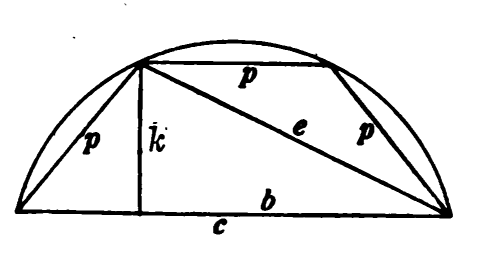
\includegraphics[width=0.6\linewidth]{pdf293-a.png}\end{center}
$e^2 = b^2 + k^2 = b^2 + \{p^2 - (c-b)^2\} = p^2 + cp$ である。すなわち、上で得た二辺折線の公式を適用すれば $cd^2 - 3d^2p + 4p^3 = 0$ を得る。これから、$q = c^2/d^2$, $x = p^2/d^2$ と書けば
\[
-q + 9x - 24x^2 + 16x^3 = 0,
\]
が従い、三次方程式に対する \emph{tetsujutsu} 展開によって
\[
p^2 = \frac{c^2}{9} + \frac{2.8q}{6.9}D_0 + \frac{5.14q}{9.15}D_1 + \frac{8.20q}{12.21}D_2 + \frac{11.36q}{15.27}D_3 + \cdots.
\]

\scanpage{0294}{印刷頁 280}
4角線については、2角線に対する展開を取り、その結果得られる方程式に二度目の展開を施す。こうして
\[
p^2=\frac{c^2}{4^2}+\frac{3.5q}{6.8}D_0+\frac{7.9q}{10.12}D_1+\frac{11.13q}{14.16}D_2+\frac{15.17q}{18.20}D_3+\cdots.
\]
を得る。

これら三つの級数の数係数の比は
\[
\begin{array}{lllllll}
\frac{1}{2^2}, & \frac{1.6}{4.6}, & \frac{3.10}{6.10}, & \frac{5.14}{8.14}, & \frac{7.18}{10.18}, & \frac{9.22}{12.22}, & \ldots,\\[1mm]
\frac{1}{3^2}, & \frac{2.8}{6.9}, & \frac{5.14}{9.15}, & \frac{8.20}{12.21}, & \frac{11.26}{15.27}, & \frac{14.32}{18.33}, & \ldots,\\[1mm]
\frac{1}{4^2}, & \frac{2.10}{8.12}, & \frac{7.18}{12.20}, & \frac{11.26}{16.28}, & \frac{15.34}{20.36}, & \frac{19.42}{24.44}, & \ldots.
\end{array}
\]
である。

これらの数が作られる法則を見いだすのは難しくない。というのは、第一行において数
\[
1,\ 3,\ 5,\ 7,\ 9,\ \ldots;\ 4,\ 6,\ 8,\ 10,\ 12,\ \ldots;\ 6,\ 10,\ 14,\ 18,\ 22,\ \ldots
\]
が等差数列をなして進み、残りの行についても同様だからである。こうして、$n$ 角線に対応する比は
\begin{gather*}
\frac{1}{n^2},\quad \frac{(1n-1).2(1n+1)}{2n.3n},\quad \frac{(2n-1).2(2n+1)}{3n.5n},\quad \frac{(3n-1).2(3n+1)}{4n.7n}\\
\frac{(4n-1).2(4n+1)}{5n.9n},\ \ldots,
\end{gather*}
すなわち
\[
\frac{1}{n^2},\ \frac{2(1^2n^2-1)}{2.3n^2},\ \frac{2(2^2n^2-1)}{3.5n^2},\ \frac{2(3^2n^2-1)}{4.7n^2},\ \frac{2(4^2n^2-1)}{5.9n^2},\ \frac{2(5^2n^2-1)}{6.11n^2},\ \ldots.
\]
となることがわかるであろう。

したがって $n$ 角線については
\[
p^2=\frac{c^2}{n^2}+\frac{4q}{3.4}\left(1^2-\frac{1}{n^2}\right)D_0+\frac{4q}{5.6}\left(2^2-\frac{1}{n^2}\right)D_1+\frac{4q}{7.8}\left(3^2-\frac{1}{n^2}\right)D_2+\cdot\cdot
\]
を得る。

この級数に \emph{tetsujutsu} 展開の方法を適用すれば、$\alpha=c^2/d^2$ と書いて
\[
p=\frac{c}{n}+\frac{\alpha}{2.3}\left(1^2-\frac{1}{n^2}\right)D_0+\frac{\alpha}{4.5}\left(2^2-\frac{1}{n^2}\right)D_1+\frac{\alpha}{6.7}\left(3^2-\frac{1}{n^2}\right)D_2+\cdots
\]
を得る。

次に、$d$, $n$ および $p$ によって $c^2$ と $c$ を求めるために、Hasegawa は上で得た式を
\begin{multline*}
-n^2p^2+c^2+\frac{(1^2-\varkappa)c^4}{3d^2}+\frac{2(1^2-\varkappa)(2^2-\varkappa)c^6}{5.3^2d^4}+\frac{(1^2-\varkappa)(2^2-\varkappa)(3^2-\varkappa)c^8}{35.3^2d^6}\\
+\frac{(1^2-\varkappa)\ldots(4^2-\varkappa)c^{10}}{7.5^2.3^4d^8}+\frac{2(1^2-\varkappa)\ldots(5^2-\varkappa)c^{12}}{77.5^2.3^5d^{10}}+\cdots=0,
\end{multline*}
の形に取る。ここで $\varkappa=\frac{1}{n^2}$ である。これは無限次の方程式であり、これを開いて $c^2$ の値を求めなければならない。いま求めることが要求されるのは、最初の

\scanpage{0295}{印刷頁 281}
\noindent 展開における六項。ここでは上の級数において、$c^2$ の最初の諸冪を六乗まで残すだけでよい。それより高い冪は、展開における求める項に影響しないからである。こうして $c^2$ についての六次方程式が得られ、その一根を \emph{tetsujutsu} 法によって開かなければならない。簡単のため、この方程式を次の形に書くことにする\footnote{Hasegawa の著作では、これはやや異なる形で与えられている。}。
\[
-t+x+\alpha x^2+\beta x^3+\gamma x^4+\delta x^5+\varepsilon x^6=0,
\]
これは次の図式のように配列される。\footnote{ここでは、絶対類、および一次、二次、\dots\ の各次の類を表すのに、記号 $0^0$, $1^0$, $2^0$, \dots\ を用いる。}

\begin{center}
\begin{tabular}{|c|c|c|c|c|c|c|}
\hline
$0^0$ & $1^0$ & $2^0$ & $3^0$ & $4^0$ & $5^0$ & $6^0$ \\
\hline
$-t$ & $1$ & $\alpha$ & $\beta$ & $\gamma$ & $\delta$ & $\varepsilon$ \\
\hline
\end{tabular}
\end{center}

第一の段階は、$-0^0\div 1^0=t$ を求める展開の第一項として取り、天元術によって数字方程式を解く場合と同じ手順に従うことである（これについては第11章を見よ）。この演算の後に残る式は、次の形をとる。

\begin{center}
\begin{tabular}{|l|c|c|c|c|c|c|}
\hline
\multicolumn{1}{|c|}{$0^0$} & $1^0$ & $2^0$ & $3^0$ & $4^0$ & $5^0$ & $6^0$ \\
\hline
$(-t$ & $1$ & $\alpha$ & $\beta$ & $\gamma$ & $\delta$ & $\varepsilon$ \\
\quad$+t)$ & $+2\alpha\mathrm{t}$ & $+3\beta t$ & $+4\gamma t$ & $+5\delta t$ & $+6\varepsilon t$ & \\
$+\alpha t^2$ & $+3\beta t^2$ & $+6\gamma t^2$ & $+10\delta t^2$ & $+15\varepsilon t^2$ & & \\
$+\beta t^3$ & $+4\gamma t^3$ & $+10\delta t^3$ & $+20\varepsilon t^3$ & & & \\
$+\gamma t^4$ & $+5\delta t^4$ & $+15\varepsilon t^4$ & & & & \\
$+\delta t^5$ & $+6\varepsilon t^5$ & & & & & \\
$+\varepsilon t^6$ & & & & & & \\
\hline
\end{tabular}
\end{center}

展開の次の項は、絶対類における $t$ の最低次の項を、$1^0$ 類の最低次の項である 1 で割り、反対の符号を付けて取ったものによって与えられる。次いで前と同じ過程を繰り返すべきであるが、いくつかの項は、求める展開における結果に影響を及ぼすことなく省いてよい。絶対項類における $t^6$ の係数に影響する項は、$1^0$, $2^0$, $3^0$ 類のそれぞれ最初の五項、三項および一項である。残りの項は

\scanpage{0296}{印刷頁 282}
\noindent 一度にすべて取り除くことができる。この簡略化した形で演算を実行すると、次の結果を得る。\footnote{ここでは簡単のため $t$ とその冪を書き記すことを省いたが、相次ぐ各行はそれぞれ $t^0$, $t^1$, $t^2$, \dots\ を掛けたものと考える。}

\begin{center}
\begin{tabular}{|l|l|l|l|}
\hline
\multicolumn{1}{|c|}{$0^0$} & \multicolumn{1}{c|}{$1^0$} & \multicolumn{1}{c|}{$2^0$} & \multicolumn{1}{c|}{$3^0$}\\
\hline
$\phantom{+}0$ & $\phantom{+}1$ & $\phantom{+}\alpha$ & $\beta^*$\\
$+0$ & $+2\alpha$ & $+3\beta^*$ & \\
$+(\alpha-\alpha)$ & $+3\beta-2\alpha^2$ & $+6\gamma-\alpha\beta^*$ & \\
$+\beta-2\alpha^2$ & $+4\gamma-6\alpha\beta$ & & \\
$+\gamma-3\alpha\beta+\alpha^2$\,\unclear{$\alpha^2$ or $\alpha^3$} & $+5\delta-(6\alpha\gamma^2-\alpha^2\beta)^*$ & & \\
$+\delta-4\alpha\gamma+3\alpha^2\beta$ & & & \\
$+\varepsilon-5\alpha\delta+6\alpha^2\gamma-\alpha^3\beta$ & & & \\
\hline
\end{tabular}
\end{center}

星印を付けた項は次の演算では必要でないので、完全には算出していない。展開の第三項は、同じ規則に従って $=(2\alpha^2-\beta)t^3$ と取る。

\noindent
\begin{minipage}[t]{0.47\linewidth}\vspace{0pt}
\begin{tabular}{|l|l|l|}
\hline
\multicolumn{1}{|c|}{$0^0$} & \multicolumn{1}{c|}{$1^0$} & \multicolumn{1}{c|}{$2^0$}\\
\hline
 & $\phantom{+}1$ & $\alpha^*$\\
$\phantom{+}At^4$ & $+2\alpha t$ & \\
$+Bt^5$ & $+(3\beta-2\alpha^2)t^2$ & \\
$+Ct^6$ & $+Dt^{3*}$ & \\
\hline
\end{tabular}
\end{minipage}\hfill
\begin{minipage}[t]{0.5\linewidth}\vspace{0pt}
これは前に行った通りである。前と同様の演算を施すと、残りの式が添付の形で得られる。ここで次のように書く。
\[
A=\gamma-3\alpha\beta+\alpha^3+(4\alpha^2-2\alpha\beta),
\]
\[
\begin{aligned}
B&=\delta-4\alpha\varepsilon+3\alpha^2\beta+(8\alpha^2\beta\\
&\qquad-3\beta^2-4\alpha^4),
\end{aligned}
\]
\end{minipage}
\[
\begin{gathered}
C=2-5\alpha\delta+6\alpha^2\gamma-\alpha^3\beta+(-4\beta\gamma-3\alpha^2\beta+8\alpha^2\gamma+7\alpha\beta^2+6\alpha^2\\
-14\alpha^3\beta),\\
D=4\gamma-6\alpha\beta+(3\alpha^2-\alpha\beta).
\end{gathered}
\]

\noindent
\begin{minipage}[t]{0.62\linewidth}\vspace{0pt}
\begin{tabular}{|l|c|}
\hline
\multicolumn{1}{|c|}{$0^0$} & $1^0$\\
\hline
$(A-A)t^4$ & $1$\\
$(+B-2\alpha A)t^5$ & $2\alpha t$\\
$\{+\gamma-(3\beta-2\alpha^2)A\}t^6$ & $(+3\beta-2\alpha^2)t^{2*}$\\
\hline
\end{tabular}
\end{minipage}\hfill
\begin{minipage}[t]{0.35\linewidth}\vspace{0pt}
\setlength{\parindent}{1.5em}
\indent 展開の第四項は $-At^4$ であり、演算は添付に示すように進む。

第五項は $-(B-2\alpha A)t^5$ であり、
\end{minipage}

\noindent 対応する演算を行った後、次の式を得る。

\scanpage{0297}{印刷頁 283}
\begin{center}
\begin{tabular}{|c|c|}
\hline
$0^0$ & $1^0$\\
\hline
$(B-2\alpha A)t^5-(B-2\alpha A)t^5$ & $1$\\
$+\{C-(3\beta-2\alpha^2)A-2\alpha(\beta-2\alpha A)\}t^6$ & $+\,2\alpha t$\\
\hline
\end{tabular}
\end{center}

すると、必要な次の、そして最後の項は、明らかに次のようになる。
\[
\{-C+(3\beta-2\alpha^2)A+2\alpha(B-2\alpha A)\}t^6.
\]

こうして得られた結果は、書き直すと次の形になる。
\[
\begin{aligned}
c^2=p^2n^2&-\frac{4k}{3.4}(n^2-1^2)D_0+\frac{4k}{5.6}(n^2-2^2)D_1-\frac{4k}{7.8}(n^2-3^2)D_2\\
&+\frac{4k}{9.10}(n^2-4^2)D_3-\frac{4k}{11.12}(n^2-5^2)D_4+\cdots,
\end{aligned}
\]
ここで $k=p^2/d^2$ である。

以上が、一世紀前の旧日本の数学者が用いた級数の反転の方法である。

この級数に \emph{tetsujutsu} の方法を適用すれば、
\[
c=pn-\frac{k}{2.3}(n^2-1^2)D_0+\frac{k}{4.5}(n^2-3^2)D_1-\frac{k}{6.7}(n^2-5^2)D_2+\cdots
\]
を得る。

以上に述べたことは、日本の数学の重要な分科の一つである \emph{kakujutsu}、すなわち多角形の理論に適用できる。たとえば、正 $n$ 角形の外接円の半径 $r$ の平方を求めるのに、Hasegawa は次のように進める。\footnote{この手続きは部分的にしか厳密でない。}すでに得たところから、次を得る。
\[
\begin{aligned}
p^2=\frac{c^2}{n^2}&+\frac{4}{3.4}\left(1^2-\frac{1}{n^2}\right)\frac{c^2}{d^2}D_0+\frac{4}{5.6}\left(2^2-\frac{1}{n^2}\right)\frac{c^2}{d^2}D_1\\
&+\frac{4}{7.8}\left(3^2-\frac{1}{n^2}\right)\frac{c^2}{d^2}D_2+\cdots.
\end{aligned}
\]
ところで、六角形は、その辺が外接円の直径に対して通約可能な比をもつ唯一の多角形である。そこで著者は、説明のために六角形を取る。正三角形の辺は十八角形の六辺が内接する弧の弦であり、正方形の辺は二十四角形の六辺が内接する弧の弦であり、五角形の辺は三十角形の六辺が内接する弧の弦であり、以下同様であることがわかるであろう。したがって、もし $m$ を……の数とすれば

\scanpage{0298}{印刷頁 284}
辺をもつならば、$\frac{m}{b}$\unclear{$b$ or $6$} は六角形の一辺に対する弧に内接する等しい弦の数であり、その辺は $=\frac{d}{2}\cdot$ である。したがって $c=\frac{1}{2}\,d$ と取れば、$c^2/d^2=\frac{1}{4}$ となり、また $1/n^2=6^2/m^2=k$ とおく。こうして上の級数は
\[
\frac{p^2}{(\frac{1}{2}d)^2}=k+\frac{1^2-k}{3.4}\,k+\frac{2^2-k}{5.6}\,D_1+\frac{3^2-k}{7.8}\,D_2+\frac{4^2-k}{9.10}\,D_3+\cdots,
\]
となり、これから $\left(\frac{d}{2}\right)^2=r^2=p^2/(\text{級数})$ が従う。

この推論は、もともと辺の数が 6 の倍数である多角形の場合について試みられたものである。しかし著者は、何らそれ以上の考察を加えずに、ためらうことなくこれを一般の場合に適用している。もちろん、これはわれわれの著者に限ったことではなかった。旧派の日本の数学者たちは、つねにこのような推論の緩さに慣れていたのである。彼らが目指したのは最終的な結果のみであって、これらの結果に至る予備的な考察は、単にその目的に役立つ道具とみなされていたにすぎなかった。

正 $m$ 角形の外接円の半径 $r$ の公式は
\[
r=p/\left\{\frac{6}{m}+\frac{(1^2-k)}{4.6}\,D_0+\frac{(3^2-k)}{8.10}\,D_1+\frac{(5^2-k)}{12.14}\,D_2+\cdots\right\},
\]
と得られた。これは Kurushima Yoshita が得たものと同じ式である。\footnote{Fukuda Riken の \emph{Sampō Tamatebako}、一八七九年。}

\begin{center}
第41章。\\[1mm]
HASEGAWA の KYŪSEKI TSŪKŌ における\\
楔形截片について。
\end{center}
\phantomsection\addcontentsline{toc}{subsection}{第41章　HASEGAWA の KYŪSEKI TSŪKŌ における 楔形截片について}

1. 円理に関する最良の論著は、疑いもなく Hasegawa Kō の \emph{Kyūseki Tsūkō} であった。これは Hasegawa の手によって書かれたが、一八四四年にその門人 Uchida Kyūmei の名で刊行された。この書物には円形の楔についての論述が含まれており、以下においてその叙述を試みることにする。

楔という主題は決して新しいものではなかった。古代の \emph{Chiu-chang}、すなわち\emph{九つの章}の問題のいくつかはこれに関わるものであり、その後さまざまな他の著者がこれに続いた。一七世紀および一八世紀の日本の数学者たちもまた、関連する諸主題を広く研究した。円形の底をもつ楔でさえ、ここで扱う論著の刊行以前にすでに注目されていた。しかし、この主題の体系的な研究が初めて試みられたのは、Hasegawa の著作においてであった。

\scanpage{0299}{印刷頁 285}
2. Hasegawa は円楔を二つの類に分けて扱う。楔の稜は底の大きさとは無関係に任意の長さであってよいが、Hasegawa は、若干の特別な場合を除いて、稜が底円の直径に等しい\unclear{eqnal / equal}場合だけを考察する。このような楔の形成は、彼が論じているように、二通りに考えることができる。

稜に平行な底円の直径を、稜を分けるのと同じように、いくつかの等しい部分に分けるとする。これらの分点において直径に直角に縦線を引き、円周と稜の対応する分点を直線で結ぶ。そこで分割の数を限りなく増すと一つの曲面が得られ、これが一つの種の円楔である。

もう一つの種の楔は、前記の直径の上にある半円周の分割を等しく行うときに得られる。

これらの円楔は、基準の直径と稜とが矩形をなし、その平面が底の平面に垂直であるとき、直であるといわれる。斜めの楔もまた作ることができる。

楔の底は、楕円、円弓、あるいは任意の形の平面曲線で置き換えることができる。これらの楔の論究はきわめて興味深いものとなろう。それらは円楔の場合よりもはるかに複雑だからである。

二種の楔のうち、第二のものが、普通に単に楔と呼ばれるものである。Hasegawa はこの種の楔を「正規の楔」と呼び、一方、他のものは「非正規のもの」と呼ばれる。しかし彼は主として後者の種を考察する。

3. この種の直円楔または直楕円楔を底に平行な平面で切れば、切り口は楕円である。基準の直径に垂直で（楕円楔の場合には長径または短径を意味するものと解する）、その直径の一端と楔の反対側の端とを通る平面による切り口は、\emph{hōshu-yen} すなわち「\emph{hōshu} 形の円または卵形」と呼ばれる曲線である。これは後年 \emph{scnyen}\unclear{scnyen / senyen} すなわち「尖った円または尖点のある卵形」という名で呼ばれた。

平面が稜の端を通らず、その端を通る母線に沿って楔を切る場合には、切り口の形は「尖点のある卵形」に似た曲線であるが、尖端あるいは尖点をもたない。

稜上の一点を通る切り口もまた尖った端をもつ曲線であるが、この場合それは尖点ではなく結節点である。

\scanpage{0300}{印刷頁 286}
斜楔の場合にも、断面は同じ形をなす。ただ、楔の傾斜のために変形されている点だけが異なる。

もちろん、ほかの種類の断面を作ることもできる。たとえば、稜に平行な直径によって分けられた半円周または半周のいずれか一方の中点を通る断面のようなものである。

4. 以下で考察する楔は、例外的な場合を除き、すべて非正規の楔である。それゆえ簡単のため、この種の楔を単に楔と呼ぶことにする。

円楔の底面に平行な断面の面積を求めるのに、Hasegawa は次のように進める。底面の直径を
\begin{center}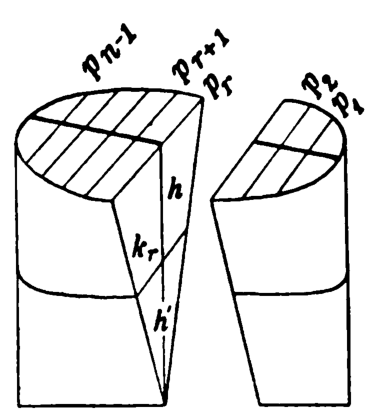
\includegraphics[width=0.6\linewidth]{pdf300-a.png}\end{center}
平行な直径 $p_1$, $p_2$, $\ldots$, $p_{n-1}$ によって $n$ 等分する。これらは直径の一端から始めて数える。これらの縦線を通る垂直断面を作る。そこで楔の高さを $h$、断面の高さを $h'$、$p_r$ に対応する断面平面の弦を $k_r$、$k_r$ の最大値（すなわち中央のもの）を $k$ で表せば、
\[
h' = \frac{hk}{d}, \quad k_r = \frac{p_r h'}{h} = \frac{p_r k}{d},
\]
を得る。ここで $d$ は稜に平行な底面の直径である。したがって断面の面積要素は $A_r = k_r \times \frac{d}{n} = \frac{p_r k}{n}$ であり、その結果、面積 $A$ は
\[
A = \lim\nolimits_{n=\infty} \sum_{r=1}^{n} A_r = k \lim \sum_{r=1}^{n} \frac{p_r}{n} = \frac{kB}{d} = \frac{kd^2\frac{\pi}{4}}{d} = kd\frac{\pi}{4},
\]
となる。ここで $B$ は底面の面積である。ところで $kd\frac{\pi}{4}$ は、$k$ と $d$ を主径とする楕円の面積である。こうして Hasegawa は、この断面が楕円であると結論する。

この考察は楕円楔の場合にも同様に適用できる。その場合には、$d'$ を $d$ に垂直な底面の直径とすれば、$k$ の値は $h' = hk/d'$ から求められ、したがって $k_r = p_r k/d'$ となる。ゆえに断面の面積は
\[
= k \cdot \frac{d}{d'} \cdot \frac{B'}{d} = k \cdot \frac{d}{d'} \cdot \frac{dd'\frac{\pi}{4}}{d} = kd\frac{\pi}{4},
\]
とすべきである。ここで $B'$ は底面の楕円の面積である。

\scanpage{0301}{印刷頁 287 (top right)}
5. 底面に平行な断面によって稜の側から切り取られる楔の部分の体積については、次を得る。
\[
V_r = \frac{1}{2}\cdot k_r h'\cdot\frac{d}{n} = \frac{p_r h k^2}{2nd},
\]
\[
\therefore\quad V = \lim\nolimits_{n=\infty}\sum_{r=1}^{n} V_r = \lim\frac{hk^2}{2d}\sum_{r=1}^{n}\frac{p_r}{n} = \frac{hk^2}{2}\times\frac{\pi}{4}.
\]

この式において $k = d$ と書けば、円楔の全体積 $= \frac{hd^2}{2}\times\frac{\pi}{4}$ を得る。

\begin{center}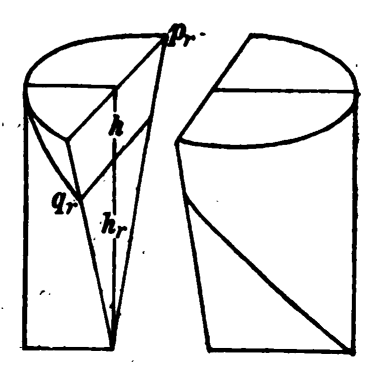
\includegraphics[width=0.6\linewidth]{pdf301-a.png}\end{center}

6. 次に、稜の一端と、それに平行な底面の直径の反対側の端とを通り、かつこれらの平行線の平面に垂直な平面によって切り取られる楔の一部分の体積を求めるには、前の場合のそれ\unclear{tbat / that}に類似した作図を試みなければならず、図のように記号を定めれば、$h_r$ と $q_r$ の式は $h_r = \frac{h}{n}\times r$ および $q_r = \frac{p_r\times r}{n}$ となる。ゆえに体積の要素は次のようになる。
\[
V_r = h_r q_r\times\frac{d}{n} = \frac{hp_r r^2 d}{n},
\]
\[
\therefore\quad V = hd\lim\sum\frac{p_r r^2}{n^3} = \frac{5hd^2}{32}\times\frac{\pi}{4}.
\]

7. \emph{hōshuyen} とは、円楔または楕円楔を、直径の一端点と稜の反対側の端とを通って切った断面から生ずる曲線である。これら二つの端点を結ぶ直線を曲線の縦軸と呼び、その中央においてそれに垂直な軸を横軸と呼ぶ。後者は、明らかなように、稜に平行な直径に共役な底面の直径の、半分の長さ\unclear{length / leugth}をもつ。

\emph{hōshuyen} に関する計算は、楔の底面が円であっても楕円であっても、同じであるか、あるいは類似している。

曲線の縦軸と横軸をそれぞれ $a$ および $b$ とする。すると \S~6 で行ったような作図において、$a$ は $n$ 等分されることになる。こうして曲線の面積の要素については次を得る。
\[
A_r = q_r\times\frac{a}{n} = \frac{a\times r\times p_r}{n^2},
\]
\[
\therefore\quad A = a\lim\nolimits_{n=\infty}\sum_{r=1}^{n}\frac{rp_r}{n^2} = a\left(\frac{d}{2}\cdot\frac{\pi}{4}\right) = ab\,\frac{\pi}{4},
\]
これは表の助けを借りて計算されるとおりである。

\scanpage{0302}{印刷頁 288}
8. 底面の直径の端と稜の中点とを通る断面の面積を求めるには、この二点を結ぶ線を $a$ とし、直径に垂直な平面によって $a$ を $2n$ 等分する。これらの平面によって得られる底面の弦を、中心から数えて $p_1, p_2, \ldots$ で表し、$a$ の分点から稜へ引いた線を $h_1, h_2, \ldots,$ で表し、また $p_1, p_2, \ldots$ に平行に引いた断面の弦を $c_1, c_2, \ldots$ で表す。このとき
\begin{gather*}
A_r = \frac{a}{n} \times c_r = \frac{a}{n} \times \frac{p_r h_r}{h} = a \times \frac{r}{n^2} \times p_r,\\
\therefore\quad A = a \lim\nolimits_{n=\infty} \sum \frac{rp_r}{n^2} = \frac{ad}{3}.
\end{gather*}

9. 底面の直径の端を通り、かつ直径の他端における母線上の一点を通る断面の場合には、$a$ を前と同様の長さとし、$h'$ と $h_0$ を母線の二つの部分とする。そのうち前者は底面に隣接する部分である。直径 $d$ を平行な平面によって $n$ 等分し、それらの平面と底面との交線を $p_r$ と呼ぶ。番号 $r$ は母線から直径の他端へ向かって数える。$h_1, h_2, \ldots$ を $a$ の対応する分点の高さとし、$k_r$ を前の場合と同様の量とする。このとき $a = h'^2 + d^2$ であり、また
\begin{gather*}
h_r = h_0 + \frac{rh'}{n}, \quad k_r = \frac{h_r p_r}{h} = \frac{h_0 p_r}{h} + \frac{rh' p_r}{nh}.\\
\therefore\quad A_r = k_r \times \frac{a}{n} = \frac{a}{h}\left(h_0 \times \frac{p_r}{n} + h' \times \frac{rp_r}{n^2}\right),\\
\therefore\quad A = \frac{a}{h}\left\{h_0 \lim\nolimits_{n=\infty} \sum_{r=1}^{n} \frac{p_r}{n} + h' \lim\nolimits_{n=\infty} \sum_{r=1}^{n} \frac{rp}{n^2}\right\}\\
= \frac{ad}{h}\left(h_0 + \frac{h'}{2}\right)\frac{\pi}{4} = \frac{ad}{h}\left(h - \frac{h'}{2}\right)\frac{\pi}{4}.
\end{gather*}

\begin{center}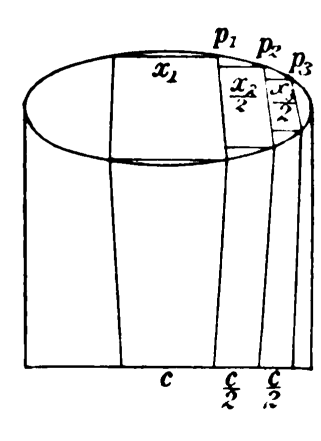
\includegraphics[width=0.6\linewidth]{pdf302-a.png}\end{center}

10. 底円の円周を等分することから生じる円楔もまた考察されている。このような円楔の体積を求めるには、図に示すように、底面の半円周の半分を $2n$ 等分する作図が用いられる。分点から基準の直径に直角に弦 $p_1, p_2, \ldots$ を引く。番号は中心から両側へ向かって数える。二つの等しい弦 $p_1$ の端を結ぶ弦を $x_1$ と名づけ、また垂線

\scanpage{0303}{印刷頁 289 (top right)}
$p_2, p_3, \ldots$ の端からそれぞれ $p_1, p_2, \ldots$ に下ろしたものを $\frac{x_2}{2}, \frac{x_3}{2}, \cdots$ と名づける。稜もまた $2n$ 等分されるので、各部分は $d/2n = c/2$ に等しいとする。

体積の要素 $V_r$ としては、底面が $p_r \times \frac{x_r}{2}$、稜が $\frac{c}{2}$ で、垂直の高さが円楔のそれと同じ、すなわち $h$ である直線楔の体積の二倍を取る。したがって $V_r = \frac{1}{6}hp_r(2x_r + c)$ である。

\begin{center}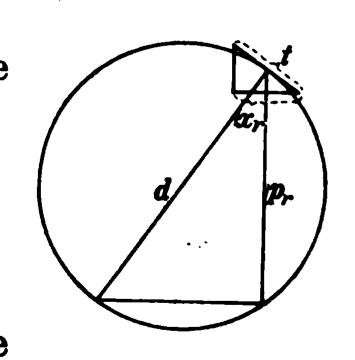
\includegraphics[width=0.6\linewidth]{pdf303-a.png}\end{center}

いま、添付のように図を描いたとする。明らかに次が成り立つ。
\[
p_r : d = x_r : t,
\]
すなわち
\[
t = \frac{d\,x_r}{p_r}.
\]
しかし、円周の分割の等しい部分（すなわち、われわれが分割した部分の二倍）は $t$ の極限値とみなしうるから、次のように書くことができる。
\[
t = \frac{d\pi}{2} \times \frac{1}{n}, \quad\text{また}\quad \therefore\ c = \frac{d}{n} = \frac{2t}{\pi}.
\]

$c$ と $t$ のこれらの値を $V_r$ に代入すると、それは
\[
V_r = \frac{1}{6}hp_r\left(2x_r + \frac{2t}{\pi}\right) = \frac{1}{3}hx_r\left(p_r + \frac{d}{\pi}\right),
\]
となり、これから、畳む演算すなわち積分によって次を得る。
\[
\begin{aligned}
V &= \frac{h}{3}\lim\nolimits_{n=\infty}\sum_{r=1}^{n} x_r p_r + \frac{hd}{3\pi}\lim\nolimits_{n=\infty}\sum_{r=1}^{n} x_r\\
&= \frac{h}{3}\left(d^2 \times \frac{\pi}{4}\right) + \frac{hd}{3\pi}(d) = \frac{hd^2}{3}\left(\frac{\pi}{4} + \frac{1}{\pi}\right).
\end{aligned}
\]

11. この種の円楔を底面に平行に切った断面の面積は、次のようにして求められる。このために Hasegawa は \S~10 と同じ作図を行い、それによって、底面における $p_r$ と $x_r$ に対応する断面上の長さを、それぞれ $k_r$ と $y_r$ で表す。$h'$ を断面の稜からの垂直距離とし、$k$ を稜に垂直なその直径とする。ここで
\[
d : p_r = k : k_r, \quad \therefore\ k_r = \frac{p_r k}{d}, \quad\text{および}\quad h' = \frac{hk}{d};
\]
であり、また
\[
(c - x_r) : (c - y_r) = h : h', \quad\text{すなわち}\quad c - y_r = \frac{h'(c - x_r)}{h},
\]

\scanpage{0304}{印刷頁 290 (top left)}
\noindent これより
\[
y_r = c - \frac{h'(c-x_r)}{h} = c - \frac{ck}{d} + \frac{x_r k}{d}.
\]
を得る。

前節と同様に $c = 2t/\pi$, $tp_r = dx_r$ と書けば、面積の要素について
\[
\begin{aligned}
A_r &= y_r k_r = \frac{kp_r}{d}\left(c - \frac{ck}{d} + \frac{x_r k}{d}\right) = \frac{2x_r k}{\pi} - \frac{2x_r k^2}{d\pi} + \frac{x_r p_r k^2}{d^2},\\
\therefore\ A &= \frac{2k}{\pi}\left(1 - \frac{k}{d}\right)\lim\nolimits_{n=\infty}\sum x_r + \frac{k^2}{d^2}\lim\nolimits_{n=\infty}\sum x_r p_r\\
&= \frac{2k}{\pi}(d-k) + \frac{k^2\pi}{4}.
\end{aligned}
\]
を得る。

12. 断面によって切り取られる楔形の部分の体積については、要素を $=\frac{1}{6}h'k_r(2y_r + c)$ と取り、したがって体積
\[
V = \lim\nolimits_{n=\infty}\sum_{r=1}^{n}\frac{h'k_r}{6}(2y_r + c) = \frac{hk}{3}\left(\frac{k}{\pi} + \frac{A}{d}\right),
\]
を得る。ここで $A$ は断面\unclear{section / sectiou}の面積である。

\begin{center}
第42章。\\[1mm]
魔方陣。
\end{center}
\phantomsection\addcontentsline{toc}{subsection}{第42章　魔方陣}

魔方陣と魔円陣は中国で研究され\unclear{stŭdied / stūdied / studied}、たとえば一五九三年の Ch'êng Tai-wei の \emph{Suan-fa T'ung-tsung} を挙げることができる。この書は日本に伝えられ、数学研究の勃興をもたらした。日本人\unclear{Japanese / Japane3e}もまた、見たところ\unclear{appareutly / apparently}この中国の大家から借用して、これらの主題を研究した。\footnote{Smith と Mikami の \emph{History} を見よ。そこには一七世紀におけるこの主題についていくらかのことが述べられている。}この主題は日本の数学者たちの好んだ題目の一つをなした。ここでは一八世紀および一九世紀に現れる魔方陣の一、二の例について述べることにする。

\emph{Kyūshi Ikō} すなわち「Kurushima の遺稿」には、奇数次の魔方陣を作る方法が含まれている。要素の個数を $n^2$ とすれば、数 $1$, $n^2$, $n$, $(n^2 + 1 - n)$ および $\frac{1}{2}(n^2 + 1)$ は図のうち左のものに示すように配置され、そしてわれわれが埋めなければならないのは

\scanpage{0305}{印刷頁 291 (top right)}
対角線 $CD$ に沿う升目を、$n$ の逐次の倍数だけ $C$ の方へ減少し $D$ の方へ増加する数で満たす。次の段階は、
\begin{center}
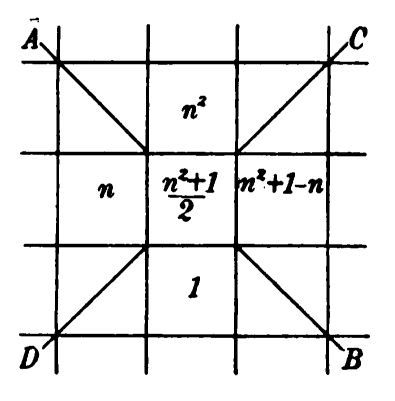
\includegraphics[width=0.3\linewidth]{pdf305-a.png}\qquad
\begin{tabular}[b]{|c|c|c|c|c|c|c|}
\hline
22 & 47 & 16 & 41 & 10 & 35 & 4\\ \hline
5 & 23 & 48 & 17 & 42 & 11 & 29\\ \hline
30 & 6 & 24 & 49 & 18 & 36 & 12\\ \hline
13 & 31 & 7 & 25 & 43 & 19 & 37\\ \hline
38 & 14 & 32 & 1 & 26 & 44 & 20\\ \hline
21 & 39 & 8 & 33 & 2 & 27 & 45\\ \hline
46 & 15 & 40 & 9 & 34 & 3 & 28\\ \hline
\end{tabular}
\end{center}
$n$ から $n^2$\unclear{$n^2$ / $n^3$} に至る線と、1 から $(n^2+1-n)$ に至る線とに沿って、$CD$ に沿う場合と同じ法則に従って満たすことである。次いで、対角線 $AB$ およびそれに平行な線に沿う升目は、$A$ の方向へは一ずつ減少し、$B$ の方向へは一ずつ増加するように満たされる。図のうち右のものは、この仕方で作られた七方陣を表す。

一七八一年の Murai Chūzen の \emph{Sampō Dōshimon} は、印刷された著作の中で魔方陣の一般的方法を記述した最初の機会であり、その先人たち、Seki, Aoyama, Matsunaga などの著述は、すべて写本の中に記録されているにすぎなかった。Murai による奇方陣の作り方を、$5^2$ 個の要素の場合について例示しよう。一方の対角線に沿う升目に数 $\frac{n+1}{2}+1=3$ を配置し、一ずつ増加または減少する他の数を、添付の図のうち第一のものに示すように、この対角線に平行な線に沿って配置する。その図ではこれらの数をローマ数字で表してある。同じ配置の仕方を他方の対角線およびそれに平行な線に沿っても行い、これをアラビア数字で表す。図のうち第二のものは、自然数を自然の順序に並べた配列
\begin{center}
\begin{tabular}[b]{|c|c|c|c|c|}
\hline
$\mathrm{IV}_3$ & $\mathrm{V}_2$ & $\mathrm{I}_1$ & $\mathrm{II}_5$ & $\mathrm{III}_4$\\ \hline
$\mathrm{V}_4$ & $\mathrm{I}_3$ & $\mathrm{II}_2$ & $\mathrm{III}_1$ & $\mathrm{IV}_5$\\ \hline
$\mathrm{I}_5$ & $\mathrm{II}_4$ & $\mathrm{III}_3$ & $\mathrm{IV}_2$ & $\mathrm{V}_1$\\ \hline
$\mathrm{II}_1$ & $\mathrm{III}_5$ & $\mathrm{IV}_4$ & $\mathrm{V}_3$ & $\mathrm{I}_2$\\ \hline
$\mathrm{III}_2$ & $\mathrm{IV}_1$ & $\mathrm{V}_5$ & $\mathrm{I}_4$ & $\mathrm{II}_3$\\ \hline
\end{tabular}\quad
\begin{tabular}[b]{c|c|c|c|c|c|}
\multicolumn{1}{c}{} & \multicolumn{1}{c}{1} & \multicolumn{1}{c}{2} & \multicolumn{1}{c}{3} & \multicolumn{1}{c}{4} & \multicolumn{1}{c}{5}\\ \cline{2-6}
1 & 1 & 6 & 11 & 16 & 21\\ \cline{2-6}
2 & 2 & 7 & 12 & 17 & 22\\ \cline{2-6}
3 & 3 & 8 & 13 & 18 & 23\\ \cline{2-6}
4 & 4 & 9 & 14 & 19 & 24\\ \cline{2-6}
5 & 5 & 10 & 15 & 20 & 25\\ \cline{2-6}
\end{tabular}\quad
\begin{tabular}[b]{|c|c|c|c|c|}
\hline
14 & 10 & 1 & 22 & 18\\ \hline
20 & 11 & 7 & 3 & 24\\ \hline
21 & 17 & 13 & 9 & 5\\ \hline
2 & 23 & 19 & 15 & 6\\ \hline
8 & 4 & 25 & 16 & 12\\ \hline
\end{tabular}
\end{center}

\scanpage{0306}{印刷頁 292 (top left)}
\noindent そして、その行と列を、そこに示されている通りに名づける。次に第三の方陣を作り、その升目を第一の方陣の升目に対応させて埋めるが、その際、第一の方陣においてローマ数字とアラビア数字がそれぞれ示す行と列の番号をもつ、第二の方陣の要素をこの目的に用いる。たとえば、第一の方陣で III と 5 と記された升目に対応する第三の方陣の升目には、第二の方陣の第3行第5列にある項 23 が入れられる。こうして作られた方陣は、要求通りに魔方陣となる。同じ規則は、要素の数がいくつの場合にも適用できるであろう。

\begin{center}
\begin{tabular}{|c|c|c|c|}
\hline
$1_{\mathrm{IV}}$ & $2_{\mathrm{I}}$ & $3_{\mathrm{I}}$ & $4_{\mathrm{IV}}$ \\
\hline
$2_{\mathrm{III}}$ & $4_{\mathrm{II}}$ & $1_{\mathrm{II}}$ & $3_{\mathrm{III}}$ \\
\hline
$3_{\mathrm{II}}$ & $1_{\mathrm{III}}$ & $4_{\mathrm{III}}$ & $2_{\mathrm{II}}$ \\
\hline
$4_{\mathrm{I}}$ & $3_{\mathrm{IV}}$ & $2_{\mathrm{IV}}$ & $1_{\mathrm{I}}$ \\
\hline
\end{tabular}
\end{center}

偶数方陣については、Murai は一例を与えるだけであり、そこでは図に示した通りの配置が何の説明もなく示されている。しかし、これを奇数方陣の場合の説明と比べれば、構成の法則は明らかであろう。

一八四〇年の Gokai Ampon の \emph{Sampō Semmon-shō} もまた、魔方陣を作る一つの方法を扱っている。彼は魔方陣が三種、すなわち奇数、複偶数、単偶数に分類されるものと考える。奇数方陣を作るには、Gokai は 1 を中央の升目より一つ下の升目に置き、そこから
\begin{center}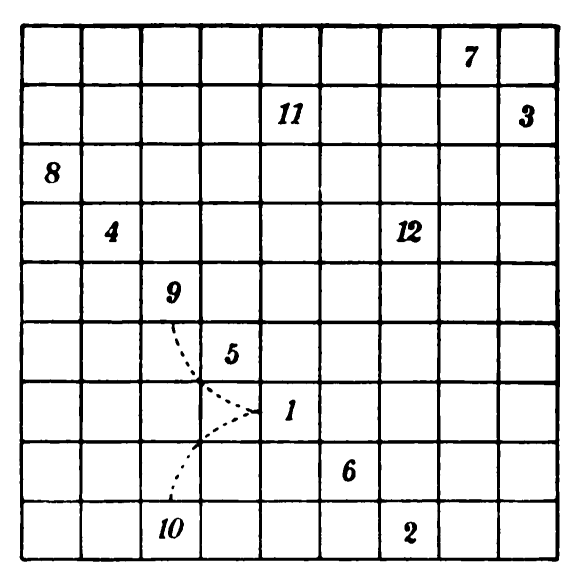
\includegraphics[width=0.6\linewidth]{pdf306-a.png}\end{center}
右下へ向かう斜めの線に沿って進み、升目を数 2, 3, \dots で埋めていく。しかし、最下の行に沿った位置または右側に沿った位置に来たときには、次の縦の列の最上の升目、または次の横の行の最も左の升目へ移り、同じ仕方で続ける。このようにして、すでに埋められた升目に来たときには、その左下に隣接する升目へ行かなければならない。1 を中央の升目より二つ以上下の升目に置く場合にも、同じ作り方を採用することができる。この場合には、その手順において毎回同じ数の位置を飛び越さなければならない。添付の図は、この作り方の性質を例示するであろう。

$(4n)^2$ 個の要素をもつ複偶数方陣を作るには、それがいくつかの四方陣から成るものと考える。これらの基本となる四方陣に、対角線が引かれているとする。次に、最初の $(4n)^2$ を並べ

\scanpage{0307}{印刷頁 293}
\noindent 自然数を添付のように二つの図式に配列し、正方形の升目を、これらの集合の第一のものの対応する項のうち

\begin{center}
\begin{tabular}{|cccc|}
\hline
1 & $4n+1$ & $2.4n+1$ & . \\
2 & $4n+2$ & $2.4n+2$ & $\vdots$ \\
$\vdots$ & $\vdots$ & $\vdots$ & $\vdots$ \\
$4n$ & $2.4n$ & $3.4n$ & $\vdots$ \\
\hline
\end{tabular}
\qquad\qquad
\begin{tabular}{|cccc|}
\hline
$\vdots$ & $3.4n$ & $2.4n$ & $4n$ \\
$\vdots$ & $\vdots$ & $\vdots$ & $\vdots$ \\
$\vdots$ & $2.4n+2$ & $4n+2$ & 2 \\
. & $2.4n+1$ & $4n+1$ & 1 \\
\hline
\end{tabular}
\end{center}

\noindent いま述べた対角線の下に来るものと、第二のものの項のうちそのような線の下に来ないものとで満たす。その結果は魔方陣である。

単偶数方陣を作るには、Gokai はまず添付のような図を描き、対角線に沿う升目を、

\begin{center}
\begin{minipage}[b]{0.18\linewidth}\centering
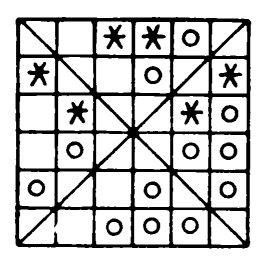
\includegraphics[width=\linewidth]{pdf307-a.png}\\
{\small $6^2$ 方陣。}
\end{minipage}\hfill
\begin{minipage}[b]{0.28\linewidth}\centering
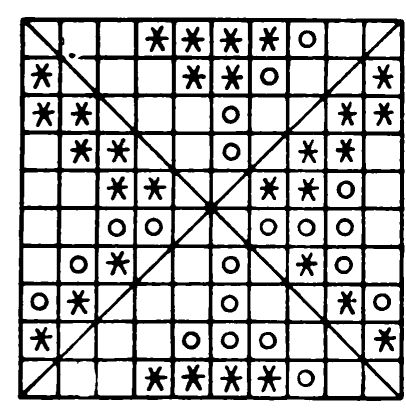
\includegraphics[width=\linewidth]{pdf307-b.png}\\
{\small $10^2$ 方陣。}
\end{minipage}\hfill
\begin{minipage}[b]{0.40\linewidth}\centering
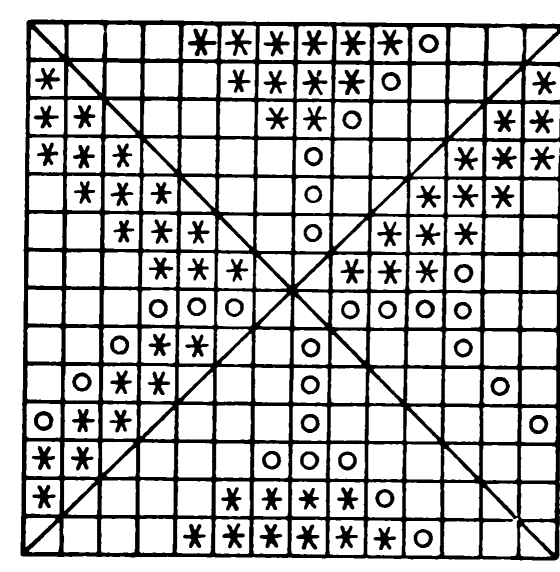
\includegraphics[width=\linewidth]{pdf307-c.png}\\
{\small $14^2$ 方陣。}
\end{minipage}
\end{center}

\noindent 複偶数方陣の場合における上の集合の第一のものと同様の順序で満たし、丸印を付した升目を、集合の第二のものにおけるのと同じ仕方で満たす。次に、ここに示すような二つの

\begin{center}
\begin{tabular}{|cccc|}
\hline
$\vdots$ & $\vdots$ & $\vdots$ & $\vdots$ \\
2 & $m+2$ & $2m+2$ & $\vdots$ \\
1 & $m+1$ & $2m+1$ & $\vdots$ \\
\hline
\end{tabular}
\qquad\qquad
\begin{tabular}{|cccc|}
\hline
$\vdots$ & $2m+1$ & $m+1$ & 1 \\
$\vdots$ & $2m+2$ & $m+2$ & 2 \\
$\vdots$ & $\vdots$ & $\vdots$ & $\vdots$ \\
\hline
\end{tabular}
\end{center}

\noindent 配列を取る。ここで $m$ は一辺の升目の数を表すものと解する。星印を付した升目（原図では黒丸）は、これらの配列の第一のものの対応する項で満たし、残りの升目は第二のものの項で満たすべきである。

\scanpage{0308}{印刷頁 294 (top left)}
\begin{center}
第43章。\\[1mm]
懸垂線。
\end{center}
\phantomsection\addcontentsline{toc}{subsection}{第43章　懸垂線}

1. 日本の著作において懸垂線に関する問題が初めて現れたのは、おそらく一八六〇年に Yasuhara と Nakasone が刊行した \emph{Sūri Shimpen} 第二巻においてであった。日本では懸垂線は \emph{suishi}、すなわち「垂れ下がる糸」と呼ばれた。ここに挙げた著作には、長さと両端点間の距離とが与えられた懸垂線について、その矢\footnote{ここでは、旧派の日本の数学者たちが従った慣用に倣って、矢（日本語で \emph{shi} または \emph{ya}）という術語を用いる。懸垂線の場合には、\emph{suishi} すなわち「垂れ下がる矢」という語も用いられた。それは曲線の高さであるから、その意味は明らかであろう。}の長さを求める問題が含まれている。ここでは、この問題は楕円\unclear{ellipsé (accent as printed) or ellipse (accent a blemish)}の取扱いから得られる考察によって解かれている。この解法はきわめて粗雑なものであった。\footnote{Ōmura の \emph{Suishi Kigen} に対する C. Kawakita の注。}

一八六二年、Hagiwara Teisuke は \emph{Sampō Höyen-kan}\unclear{Höyen (diaeresis as printed) or Hōyen (broken macron)} を刊行し、その中で、曲線の長さが与えられたとき、等しい高さの二点の間に懸けられた懸垂線の垂れ下がる矢の長さを求める問題を与えた。両端間の距離 $= a$、懸垂線の矢 $= b$ と書くと、Hagiwara が与えた解法の規則は次の級数に相当する。
\[
\begin{gathered}
\frac{1}{6s}\Bigl[(s+a)\sqrt{s^2-a^2}+\frac{(s-a)^2}{2}+\frac{1}{3a}\Bigl\{D_0-(s-a)^3\\
+(1-m)\Bigl(D_0-\frac{1}{5}\,m\,D_1-\frac{1}{7}\,m\,D_2-\frac{3}{9}\text{\unclear{3/9 or 8/9}}\,m\,D_3-\frac{5}{11}\,n\,D_4-\ldots\Bigr)\Bigr\}\Bigr],
\end{gathered}
\]
ここで $D_0=(s^2-a^2)\sqrt{s^2-a^2}$, $m=\frac{s-a}{s+a}$ であり、また $D_0$ および $D_1, D_2, \ldots$ は原項および逐次の差を表す。Hagiwara の解法は説明なしに与えられた。

2. Hagiwara の著作の刊行からしばらく後、Ōmura Isshū は写本 \emph{Suishi Kigen} を著し、その中に懸垂線に関する自らの研究の成果を収めた。彼の著作には一八六七年第六月の日付がある。一八六八年第二月には、Ōmura と Kagami Mitsuteru がさらに研究を進めた。以下に、これらの成果のいくつかを示す。\footnote{一八七四年の日付のある C. Kawakita の \emph{Suishi Kigen} 写本。}

両端点間の距離 $a$ と曲線の長さ $s$ によって懸垂線の矢 $b$ を求めるために、Ōmura は

\scanpage{0309}{印刷頁 295}
\noindent 添付の通りの図。ここでは縦線を等間隔 $\left(\frac{1}{2}\,l = a/2n\right)$ に引き、水平な平行線を、図中で $k_1$, $k_2$, \dots\ によって示される長さが次の値をもつような距離にとる。
\begin{center}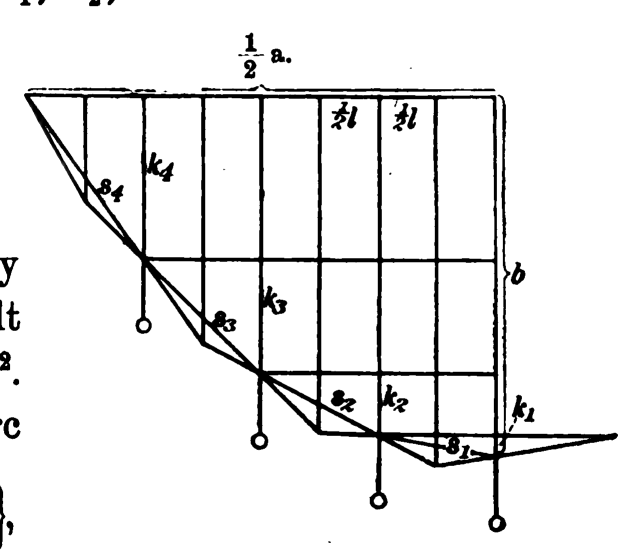
\includegraphics[width=0.6\linewidth]{pdf309-a.png}\end{center}
\[
\begin{gathered}
k_1 = k = \frac{b}{n^2},\quad k_r = (2r-1)\,k = \frac{2rb}{n^2} - \frac{b}{n^2}\\
= \frac{2bt}{n} - \frac{b}{n^2},
\end{gathered}
\]
ただし $t = r/n$ である。ここで第二項は最終的には結果に影響しないので無視してよく、したがって $k_r = 2bt/n^2$ と書くことができる。弧の要素の平方について次を得る。
\[
s_r^2 = k_r^2 + l^2 = \frac{4b^2t^2}{n^2} + \frac{a^2}{4n^2} = \frac{pa^2}{4n^2}\left\{1 - (1-t^2)\,q\right\},
\]
\[
\text{すなわち}\quad s_r = \frac{a\sqrt{p}}{2n}\left\{1 - \frac{(1-t^2)}{2}\,q - \frac{(1-t^2)^2}{8}\,q^2 - \frac{3(1-t^2)^3}{48}\,q^3 - \frac{15(1-t^2)^4}{384}\,q^4 - \cdots\right\},
\]
ここで $p = \frac{16b^2}{a^2} + 1$, $q = \frac{16b^2}{a^2}\Big/p$ と書いた。さて、折り畳みの演算、すなわち和をとって極限に移ることを行い、その結果を二倍すれば、次を得る。
\[
s = 2\lim\nolimits_{n=\infty}\sum_{r=1}^{n} s_r = a\sqrt{p}\left(1 - \frac{q}{3} - \frac{q^2}{15} - \frac{q^3}{35} - \frac{q^4}{63} - \,..\right).
\]

$b$ の値は、この式から \emph{kanrui jutsu} あるいは反復近似法を適用することによって求めることができる。すなわち、上の公式で $b$ の代りに $b' = \frac{1}{2}\sqrt{s^2 - a^2}$ を代入し、$s$ に対応する値を $s'$ とする。このとき $\frac{1}{2}(s' - s)$ は $< b' - b$ となり、しかもほぼ $= b' - b$ となるから、$b' - \frac{1}{2}(s' - s) \equiv b''$ は $> b$ である。

次に $b''$ を用いて同様に $s''$ の値を求め、以下このようにして、$s^{(i)}$ の相続く二つの値が互いに一致するまで進む。この一致する値が、求める矢の長さを表すことになる。\footnote{\emph{kanrui-jutsu} と呼ばれる近似法は、通常、Saitō Gichō によって確立され、一八三四年の彼の \emph{Sampō Yenri-kan} において初めて与えられたものと信じられている。これは超越方程式の解法に適用される方法である。しかし Wada Nei が Saitō 以前にこれを手にしていたか否かについては、われわれは確かではない。この点は今後研究されるべきである。}

3. 懸垂線の両端点が水平に位置すると仮定し、これらの端点間の距離を $a$、長さ

\scanpage{0310}{印刷頁 296}
矢が $b$ であるとする。次に、水平な弦が引かれ、その長さが $a'$ であるとする。この水平な弦によって切り取られる矢の部分の長さ $b'$ はいくらになるか。

この長さを計算するために、Ōmura は前の場合と同様の仕方で作図を行い、矢から数えて $i$ 番目の縦線が弦の端を通るものとする。そこで上と同じ記号を用いれば、
\[
b' = k + 3k + 5k + \ldots + (2i-1)k = i^2k = i^2b/n^2,
\]
となる。
\[
\text{しかるに}\qquad a' = 2i\left(\frac{a}{2n}\right) = \frac{ia}{n}, \qquad \therefore\ b' = b \times \frac{a'^2}{a^2}.
\]

4. 高さの等しくない二点の間に懸けられた懸垂線の長さもまた求めることができる。すなわち、$A$, $B$, $C$ を二つの端点および曲線の最低点の縦座標とし、$a$ を両端の水平距離とする。両端において水平な弦を作るべきである。これら\unclear{these}を $x$ および $x'$ で表す。このとき（第二の式は前節の結果である）
\[
x' = 2a - x \quad\text{および}\quad (B-C)x^2 = (A-C)x'^2,
\]
である。
\[
\therefore\quad \frac{x}{2} = \frac{a}{m+1} \quad\text{および}\quad \frac{x'}{2} = \frac{ma}{m+1}, \quad\text{ここで } m^2 = \frac{(B-C)}{A-C}.
\]

これらの値を用いて上で試みたように進めれば、これら二つの弦をもつ懸垂線の長さの諸式を得ることができる。その和の半分が求める長さを与える。すなわちそれは
\begin{multline*}
\sqrt{(A-C)^2 + \left\{\frac{a}{2(m+1)}\right\}^2} + m\sqrt{(A-C)(B-C) + \left\{\frac{a}{2(m+1)}\right\}^2} + \\
+ \frac{1}{A-C}\left\{\frac{a}{2(m+1)}\right\}^2 \sqrt{k}\left(1 - \frac{k}{3} - \frac{k^2}{5} - \frac{k^3}{7} - \ldots\right),
\end{multline*}
に等しい。ここで
\[
k = \frac{(A-C)^2\left[m\sqrt{(A-C)^2 + \left\{\frac{a}{2(m+1)}\right\}^2} + \sqrt{(A-C)(B-C) + \left\{\frac{a}{2(m+1)}\right\}^2}\right]}{\left\{\frac{a}{2(m+1)}\right\}^2 + (A-C)^2\left[m\sqrt{(A-C)^2 + \left\{\frac{a}{2(m+1)}\right\}^2} + \sqrt{(A-C)(B-C) + \left\{\frac{a}{2(m+1)}\right\}^2}\right]}.
\]

5. 次に、懸垂線の弦をその長さと矢によって求めるための、Ōmura と Kagami の研究を述べよう。

糸の三等分点から二つの重り $W_1$ と $W_2$ が吊り下げられているとする。ここでは添付のような図が与えられており、その中で $B_1K$ と $B_2K$ は重りの分力を表し、また点 $K$ については次のように記されている。「この点は……の重心である

\scanpage{0311}{印刷頁 297}
大きい方の重りと小さい方の重り。左右の重さの成分は重心へ向かう」。図には次の原理が添えられている。「図のように、大きい方の重りに対応して（長さ）$A_1$ が得られるならば、小さい方の重りに対応しては必ず $A_2$ が得られるはずである。これはてこの場合と同じである」。

\begin{center}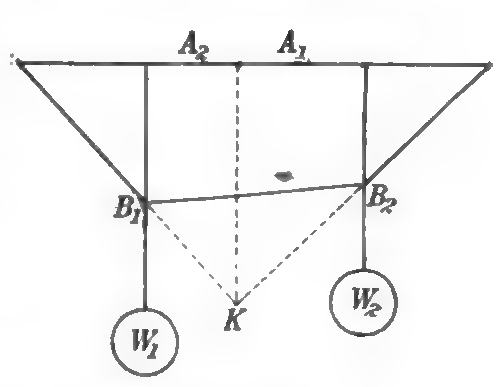
\includegraphics[width=0.6\linewidth]{pdf311-a.png}\end{center}

ここで長さの分割は、明らかに重さの逆比で行われることが意図されている。この原理は公理的な仕方で与えられている。

懸垂線の考察において、著者たちは等しい重りが等しい間隔で吊るされていると仮定し、そのときこれらの重りの間にある糸の部分はぴんと張られているものとみなされる。さて、重りは等しいと仮定されているから、相続く二つずつの重りの重心は常にそれらの中間に来る。次のように付け加えられている。「このようにして、このような考察から懸垂線の理論が生ずる。そこで、吊るされた重りによって糸が等しい部分に分けられていると考えるならば、吊るされた重りの数が無限となる極限に移るとき、懸垂線の実際の形が得られるであろう。」

\begin{center}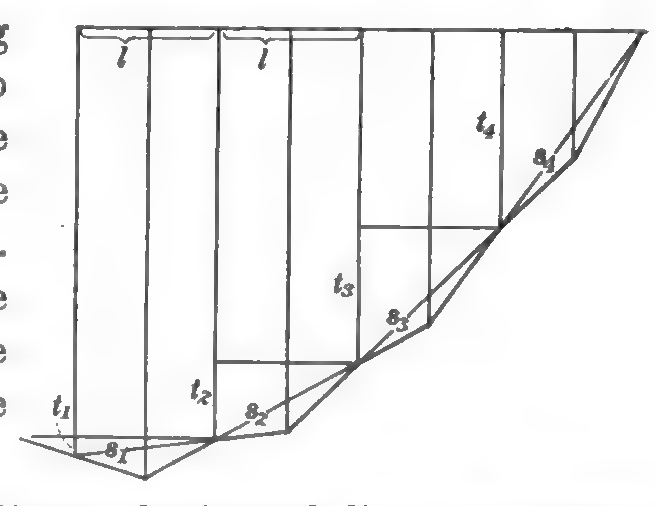
\includegraphics[width=0.6\linewidth]{pdf311-b.png}\end{center}

懸垂線を計算するために、著者たちは二種類の図を用いる。そのうちの一方の図では、矢の片側に等しい間隔 $l$ をおいて $n$ 本の縦座標が引かれる。これらの縦座標の端を順次結ぶ弦は第一、第二、\dots の弦と呼ばれ、われわれはそれらを $s_1$, $s_2$, \dots で表す。

さて、縦座標の端からそれぞれ一つ前の縦座標に向かって水平線を引くと、それらはその縦座標から部分 $t_1$, $t_2$, $t_3$, \dots を切り取る。その長さは次の通りである。
\[
t_1 = t, \quad t_2 = 3t, \quad t_3 = 5t, \quad t_4 = 7t, \dots.
\]

$s_1 = s$, $m = t_1{}^2/s^2$ と書けば、$l^2 = s^2 - t^2$ を得る。あるいは展開すれば、
\[
l = s\left(1 - \frac{m}{2} - \frac{m^2}{8} - \frac{3m^3}{48} - \frac{15m^4}{384} - \cdots\right).
\]
また次を得る $\Bigl[$ただし $p_r = 8 \cdot \frac{1}{2} r(r-1)\Bigr]$

\scanpage{0312}{印刷頁 298 (top left)}
\[
s_r^2 = (2r-1)^2 t^2 + l^2 = s^2 + \{(2r-1)^2 - 1\}\, t^2 = s^2 + 8\cdot\frac{r(r-1)}{2}\, t^2,
\]
\[
\therefore\quad \frac{s}{s_r} = 1 + \sum_{i=1}^{\infty} (-1)^i\, \frac{1.3.5\ldots(2i-1)}{2.4.6\ldots(2i)}\, p_r^i m^i.
\]

次に、もう一つの図を同様の仕方で作る。ただ一つの相違は、第一、第二、\dots{} の弦、すなわち $s_r$ をすべて $s = s_1$ に等しくすることである。この図を、二つの図の矢が一致し、また二つの弦 $s_1$ も一致するように前の図の上に重ねると、第二の図の第二の弦は第一の図の $s_2$ と部分的に一致し、第二の図の逐次の弦はそれぞれ第一の図の $s_3$, $s_4$, \dots{} に平行な位置を取る。その結果は添付の図に示す通りである。

\begin{center}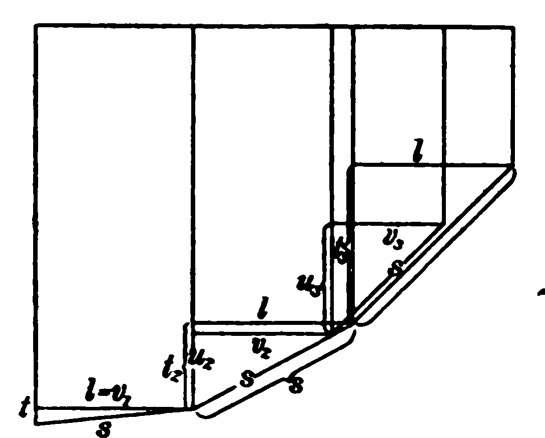
\includegraphics[width=0.6\linewidth]{pdf312-a.png}\end{center}

ここで三角形の相似によって
\[
t_r : u_r = s_r : s, \qquad \therefore\quad u_r = \frac{t_r s}{s_r} = \frac{(2r-1)\,t s}{s_r},
\]
を得る。これから、矢 $= b$ と書けば、総和を取ることによって次が導かれる。
\[
\frac{b}{t} = \sum_{r=1}^{n} \frac{u_r}{t} = \sum_{r=1}^{n} \frac{(2r-1)\,s}{s_r} = \sum_{r=1}^{n} (2r-1) \left\{ 1 + \sum_{i=1}^{\infty} (-1)^i\, \frac{1.3.5\ldots(2i-1)}{2.4.6\ldots(2i)}\, p_r^i m^i \right\},
\]
\[
\begin{array}{r@{\;}r@{\;}r@{\;}r@{\;}r@{\;}l}
\therefore\quad \dfrac{b}{s\sqrt{m}} = n^2 & {}- n^4 m & {}+ 2n^6 m^2 & {}- 3\cdot\frac{5}{3}\, n^8 m^3 & {}+ 14 n^{10} m^4 & {}- \cdots \\[1mm]
 & {}+ n^2 m & {}- 4n^4 m^2 & {}+ 10\cdot\frac{5}{3}\, n^6 m^3 & {}- 70\, n^8 m^4 & {}+ \cdots \\[1mm]
 & & {}+ 2n^2 m^2 & {}- 11\cdot\frac{5}{3}\, n^4 m^3 & {}+ 29\cdot\frac{1}{3}\, n^6 m^4 & {}- \cdots \\[1mm]
 & & & {}+ 4\cdot\frac{5}{3}\, n^2 m^3 & {}- 175\cdot\frac{1}{3}\, n^4 m^4 & {}+ \cdots \\[1mm]
 & & & & {}+ 112\cdot\frac{1}{3}\, n^2 m^4 & {}- \cdots \\[1mm]
 & & & & & {}+ \cdots
\end{array}
\]

これは $\sqrt{m} = t/s$ に対する方程式とみなすことができる。$n\sqrt{m} = x$ と書けば、それは次の形をとる。\footnote{これら二つの式の係数におけるわずかな不一致は、確かに筆写の誤りによるものである。}

\scanpage{0313}{印刷頁 299}
\[
\begin{array}{@{}r@{}l|l@{}l|l@{}l|l@{}l|l@{}}
-\frac{b}{ns}+x & {}-1 & x^3 & {}+2 & x^5 & {}-5 & x^7 & {}+14 & x^9-\cdots=0.\\[2pt]
 & {}+\frac{1}{n} & & {}-\frac{4}{n^2} & & {}+\frac{50}{3n^2} & & {}-\frac{70}{n^2} & \\[2pt]
 & \multicolumn{1}{l}{} & & {}+\frac{2}{n^4} & & {}-\frac{55}{3n^4} & & {}+\frac{406}{3n^4} & \\[2pt]
 & \multicolumn{1}{l}{} & & \multicolumn{1}{l}{} & & {}+\frac{20}{3n^6} & & {}-\frac{350}{3n^6} & \\[2pt]
 & \multicolumn{1}{l}{} & & \multicolumn{1}{l}{} & & \multicolumn{1}{l}{} & & {}+\frac{112}{3n^8} &
\end{array}
\]

$n=\infty$ の極限では、量 $sn$ は $=$ 懸垂線の長さの半分となる。したがって $b\div\text{(この長さ)}=a$ と書き、$1/n$ およびその冪を無視すれば、方程式
\[
-a+x-x^3+2x^5-5x^7+14x^9-\cdots=0,
\]
を得、ここから \emph{tetsu-jutsu} の方法による展開を適用すれば、
\[
n\sqrt{m}=a+a^3+a^5+a^7+\cdots=a/(1-a^2).
\]
を得る。

また、水平な弦 $=c$ と書けば、上の図から比例によって
\[
s_r:s=l:v_r,\quad\therefore\quad v_r=\frac{3l}{s_r},
\]
を得る。
\begin{align*}
\therefore\ \frac{\frac{1}{2}c}{l}&=\frac{1}{l}\sum_{r=1}^{n}v_r=\sum_{r=1}^{n}\frac{s}{s_r}=n+\sum_{r=1}^{n}\sum_{i=1}^{\infty}(-1)^i\frac{1.3.5\ldots(2i-1)}{2.4.6\ldots(2i)}p_r{}^i m^i\\
&=n+\sum_{i=1}^{\infty}(-1)^i\frac{1.3.5\ldots(2i-1)}{2.4.6\ldots(2i)}m^i\sum_{r=1}^{n}p_r{}^i
\end{align*}
\[
\begin{array}{@{}r@{}l|l@{}l|l@{}l|l@{}l|l@{}}
=n & {}-n^3 & \frac{4}{3.2}m & {}+3n^5 & \frac{16}{5.8}m^2 & {}-15n^7 & \frac{64}{7.48}m^3 & {}+105n^9 & \frac{256}{9.384}m^4+\cdots\\[2pt]
 & {}+n & & {}-5n^3 & & {}+42n^5 & & {}-450n^7 & \\
 & \multicolumn{1}{l}{} & & {}+2n & & {}-35n^3 & & {}+693n^5 & \\
 & \multicolumn{1}{l}{} & & \multicolumn{1}{l}{} & & {}+\phantom{0}8n & & {}-420n^3 & \\
 & \multicolumn{1}{l}{} & & \multicolumn{1}{l}{} & & \multicolumn{1}{l}{} & & {}+\phantom{0}72n &
\end{array}
\]
$=n+A_1m+A_2m^2+A_3m^3+\cdots$ とおく。

いま $l$ の代りにその展開を代入すれば、掛け合わせたのち次を得る。\footnote{ここでは因数 $\frac{1}{2}$, $\frac{1}{8}$, $\frac{3}{48}$, $\cdots$ を、それぞれの横の行のすべての項に掛けるべきものとして示してある。}

\scanpage{0314}{印刷頁 300}
\[
\begin{array}{r@{}l|l@{}l|l@{}l|l@{}l|l}
\dfrac{\frac{1}{2}c}{s} = n & {}+ A_1 & m & {}+ A_2 & m^2 & {}+ A_3 & m^3 & {}+ A_4 & m^4 + \cdots\\[1ex]
\frac{1}{2}\cdots & {}- n & & {}- A_1 & & {}- A_2 & & {}- A_3 & \\[1ex]
 & \multicolumn{1}{l}{} & \frac{1}{8}\cdots & {}- n & & {}- A_1 & & {}- A_2 & \\[1ex]
 & \multicolumn{1}{l}{} & & \multicolumn{2}{r@{}}{\frac{3}{48}\;\cdots\cdots} & {}- n & & {}- A_1 & \\[1ex]
 & \multicolumn{1}{l}{} & & \multicolumn{1}{l}{} & & \multicolumn{2}{r@{}}{\frac{15}{384}\;\cdots\cdots} & {}- n &
\end{array}
\]

ここで各 $A$ をそれぞれの値で置き換え、$4mn^2 = k$ と書けば、
\[
\begin{array}{r@{}l|l@{}l|l@{}l|l}
\dfrac{\frac{1}{2}c}{ns} = 1 & {}- \dfrac{1}{3.2} & k & {}- \dfrac{3}{5.8} & k^2 & {}- \dfrac{15}{7.48} & k^3 - \cdots.\\[2ex]
 & {}+ \dfrac{1}{3.2n^2} & & {}- \dfrac{5}{48n^2} & & {}+ \dfrac{37}{320n^2} & \\[2ex]
 & \multicolumn{1}{l}{} & & {}+ \dfrac{41}{15.128n^4} & & {}- \dfrac{387}{3840n^4} & \\[2ex]
 & \multicolumn{1}{l}{} & & \multicolumn{1}{l}{} & & {}+ \dfrac{1643}{107520n^6} &
\end{array}
\]
を得る。

いま極限 $n = \infty$ に移ると、$ns$ は $= \frac{1}{2}$（懸垂線の長さ）$= \frac{1}{2}S$ となり、$1/n$ およびその冪を含む項を無視すれば、
\[
\frac{c}{S} = 1 - \frac{k}{3.2} - \frac{3\,k^2}{5.8} - \frac{15\,k^3}{7.48} - \frac{105\,k^4}{9.384} - \cdots.
\]
を得る。

ここで、先に与えたように $k = 4mn^2 = 4a^2/(1 - a^2)^2$ であるから、$k$ の展開式の冪を上の式に代入すれば、
\[
\frac{c}{S} = 1 - \frac{2\,a^2}{3} - \frac{2.1\,a^4}{15} - \frac{2.3\,a^6}{105} - \frac{2.15\,a^8}{945} - \cdots,
\]
を得る。ここで $a = 2b/S$ である。\footnote{Ōmura と Kagami が与えた上の解析があまり厳密でないことは、容易に気づかれるであろう。著者たちは時として
\begin{center}
\begin{tabular}{@{}l@{}l@{}}
$\lim_{n=\infty} n\times s$ & ${}={}$ 懸垂線の長さの半分、\\
$\lim_{n=\infty} n\times u_r$ & ${}={}$ 懸垂線の矢
\end{tabular}
\end{center}
と置いているが、これらの関係の正当性を保証するものは何もない。したがって最終結果の真偽は確かでない。しかし、このような不厳密さは、科学的精密さを欠いてきた日本人の精神の所産の中では珍しいことではない。}

\scanpage{0315}{印刷頁 301}
\begin{center}
第44章。\\[1mm]
HAGIWARA TEISUKE。
\end{center}
\phantomsection\addcontentsline{toc}{subsection}{第44章　HAGIWARA TEISUKE}

1. 旧日本の学派に属する最後の大数学者は、確かに Hagiwara Teisuke であった。彼はこの学派の末期にその進歩に大いに寄与し、また同時代の旧学派の数学者たちの最良の代表者と見なして差し支えないので、ここで彼の生涯と業績について幾らか述べておかなければならない。そのうえ、私は彼の存命中にこの人を知っていた。実際に言葉を交わすことによって、私は彼の考えについて多くのことを知り得た。彼が私の心に残した印象は、鮮やかな像としてこれまで常に私の記憶にとどまってきたし、これからも常にとどまり続けるであろう。私が初めて彼に会ったとき、彼はすでに非常に高齢であった。そして彼は、西洋流の学問の影響があまねく行きわたっていることに失望して、二〇年もの間数学の研究を怠ってきたと私に語った。しかし彼は、敵対する学派の優越については何ひとつ認めようとしなかった。彼は、自分が研究してきたような複雑な問題を西洋の数学は解くことができないという信念を固く主張した。これらの扱いにくい問題の満足な解へと彼を導くのに役立ったのは、旧学派の驚くほど巧妙な工夫だけであった。活発に研究していた時期の後半には、彼は確かに積分学に接することになったが、その知識は通俗的で未消化な類のものであった。というのも、彼はいかなるヨーロッパの言語も修めておらず、また当時は日本全国に西洋の著作の満足な翻訳が一つもなかったからである。Loomis の漢訳が、おそらく彼の利用し得た最良の情報源であった。これらの事情を省みるとき、われわれは彼の態度に同情を覚える。西洋における数学の発達の実状について、彼は何も知らなかった。彼は、自らの晩年に同胞たちによって修められていた西洋の学問の進歩さえも知らなかった。これらの問題はしかじかの見地から積分学を応用することによって取り扱うことができると私が話すと、彼はただ微笑んでうなずくばかりであった。正直に言わねばならないが、彼の手によって発達した旧日本の数学の最高の到達点よりもさらに偉大な、現今のこの学問の偉大さを、私は彼に納得させることができなかった。それゆえ彼は、自分の成果が、数学の領域において人間の手または精神がかつて考案した最良の芸術的作品であるという、誤ってはいるが固い確信を抱いたまま没した

\scanpage{0316}{印刷頁 302 (top left)}
\noindent 学において、日本のものであれ外国のものであれ。これはおそらく、旧派の数学が栄えていた時代に日本が生んだほとんどすべての大数学者が抱いていた感情であった。昔の学者たちの著作の中で、同じ性質の言葉にときおり出会うことがある。

Hagiwara Teisuke は一八二八年、Seki Kōwa が生まれたのと同じ国である Kōzuke のある村に、農民の子として生まれた。幼少のころから農民として育てられ、当時の農家の子が受けるのを常とした教育のほかには、特別な教育を何も受けなかった。彼は早くに父を失い、農民として自立した。その暮らし向きは苦しかった。彼が数学を学び始めたのは一八五一年のことであった。富裕な農民であった高名な数学者 Saitō Gigi は、当時、Hagiwara の住居から十マイル離れた村で研究を続けていた。Hagiwara は教えを受けるために彼のもとへ赴いた。しかし彼は暇をもてないほど忙しかったので、休日の前夜、その日の仕事を終えてから訪ねて行き、まる一日師のもとにとどまって、その日の夜に帰るのを常とし、こうして農作業のために定められた時間を一時間たりとも費やさなかった。そのうえ、その十マイルの距離を彼はいつも徒歩で通った。彼が数学を学んだのは、このようにしてであった。

Kōzuke の国は、多くの著名な数学者を輩出したことで大いに知られている。Seki の場合は、彼がこの地で生を受けたとはいえ、生まれながらの幕府の武士であってこの国の土着の者ではないので、これを別にすれば、この国から現れた最初の数学者は、おそらく一九世紀の初めに生きた Fujita Seishin であった。Fujita と同時代の Ono Yeijū と Saitō Gichō は偉大な教師であり、とりわけ後者はよく知られている。彼らの住んでいた\unclear{dwelt / dwelt.}土地の近辺で数学の研究を刺激したのは、この二人の影響であった。Hagiwara の師は、この Saitō の子であった。Kōzuke の数学者の中では、Ichikawa Kōyei、Kemmochi Shōkō、Iwai Jūyen、Nakasone Sōhō などの名をとくに挙げることができる。

2. Hagiwara は農民であって、その数学の研究は余暇に営まれたにすぎなかったが、彼は天才、それも稀に見る天才であり、その知識はまもなく当代の最高水準に達した。数学者としての彼の経歴の第一歩は、確かに、彼の村から遠くない町 Mayebashi のある社寺に、三つの問題についての彼の結果を掲げたことであった。その掲げられた額は、彼がそこに祀られた神に奉納したまさにその場所に、今も見ることができる。それには一八五八年の日付がある。

\scanpage{0317}{印刷頁 303}
これらの問題のうちの一つは次の通りである。「球が、二つずつ相等しく、すべて平行な四つの円柱によって、直断面が図に示す通りになるように切られるとする。そこでは五つの円が四点で互いに接している。球の直径が与えられたとき、図中の斜線を施した部分に対応する球面の部分が最大となるように、図中の月形に対応する球面の部分を求めることが要求される。」

\begin{center}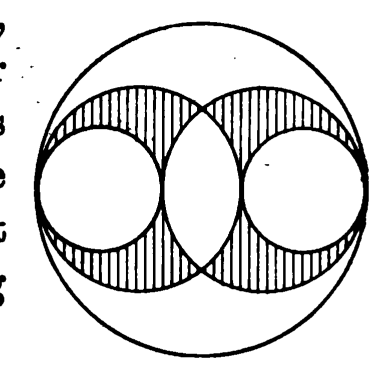
\includegraphics[width=0.6\linewidth]{pdf317-a.png}\end{center}

この問題の解として与えられた術は、次のように定式化できる。
\[
\text{(求める面積)} = \sqrt{\sqrt{20}-2}\times(\text{直径})^2.
\]

もう一つの問題は、\emph{ōyen} と呼ばれる曲線の重心に関するものである。この曲線は、他の大きな円の上を転がる小さな円の上の一点が描く軌跡として与えられ、点と円とはともに、一回転ののち点が二円の接する出発の位置に戻るような仕方で、それぞれの円に沿って右へ転がる。」

大きな円（基円）と小さな円（転がる円）の直径を $d$ と $k$ とする。
\[
A=\frac{d}{k}+1,\quad B=A^2+2,\quad C=\sqrt{\left(1-\frac{1}{B}\right)+\frac{A}{4}}-\frac{A}{4},
\]
と書けば、矢
\[
s_1=\frac{1}{2}(C+1)\quad\text{および}\quad s_2=\frac{1}{2}(C-1),
\]
と共通の弦 $c=4s_1s_2$ とをもつ弓形の面積が求められる。これらの面積を $a_1$ と $a_2$ で表す。このとき、重心を通り対称軸に垂直な直線によって切られる曲線の二つの部分の面積は
\[
A_1=(a_1B-c^3)(A+C)k^2,\quad A_2=(a_2B+c^3)(A+C)k^2,
\]
となる。ここで $A$ は尖点のある側にある部分である。

3. Hagiwara はその長い生涯のうちに非常に多くを書いた。しかし彼はそのすべてを公刊したのではなく、自ら得た結果のいくつかを印刷したにすぎない。数学に関する日本の印刷された著作の大部分は内容の薄いもので、問題と、術の形で表されたその解のための最終的な公式とが、その唯一の内容であった。考察された問題の詳しい解析が、刊行された著作の中で与えられることはまれであった。この慣習が生じたのは、確かに

\scanpage{0318}{印刷頁 304 (top left)}
\noindent 印刷の費用のためであった。というのも、そのような書物の需要はきわめて少なく、しかも版木は著者自身が用意しなければならなかったからである。Hagiwara が印刷に付した三書は、(1) 一八六二年の \emph{Sampō Hōyen-kan}、(2) 一八六七年の \emph{Sampō Yenri Shiron}、(3) 一八七八年の \emph{Yenri San-yō} であり、いずれも高次の円理に関するものである。そして晩年には、\emph{tenzan} の諸問題に関する研究の成果である最後の著作 \emph{Reikan Sampō} の出版を企てた。その出版は数年前に C.~Kawakita の手に委ねられたが、著者の存命中には刊行されなかった。著者は一九〇九年一一月二八日、八一歳の高齢で没した。この件については一つの滑稽な出来事が起こったが、私はその目撃者であった。\footnote{Hagiwara の \emph{Reikan Sampō} は、K.~Nagasawa の厚意によって一九一〇年に出版された。}

一八六八年の維新の後、Hagiwara は短期間（一八七八---八一年）Mayebashi の師範学校で教えた。また約三年間（一八八一---八四年）、Tokyo の帝国大学が行っていた歴史研究の事業に従事した。この数年を除けば、彼は常に郷里の村の家にとどまっていた。彼は農民の子として生まれ、農民として生き、農民として死んだ。貧困のうちに人生を始めたとはいえ、彼は幸いにも勤勉によっていくらかの財をなした。

彼の著述は現在、その子孫によって数多く保存されている。刊行された著作の原解析のほか、畳むことすなわち積分に用いた彼の表と、日本数学についての彼の年表とは、特別な価値をもつであろう。以下では、刊行された著作における彼の成果について、いくらか述べなければならない。これらは日本数学の最後の発達の見本となりうるであろう。

4. ここに、彼が考察した問題のいくつかを挙げる。

\emph{Hōyen-kan}\footnote{これらの問題は意味に従って述べたにすぎず、必ずしも逐語訳ではない。}（以下 H.~K. と略記する）の問題6。大円と小円の直径が与えられている（小円は大円の半分より大きくない）。中心が大円上にある小円が大円に沿って右へ回り、小円上の一点が小円に沿って同じ向きに、完全に一回転した後に出発位置に戻るような割合で動くとき、この点の軌跡である曲線をその軸のまわりに回転して得られる立体の表面積を求めることが要求される。

\scanpage{0319}{印刷頁 305}
術。大きい円と小さい円の直径をそれぞれ $d$ および $k$ とすれば、次を得る。
\[
\text{(表面積)} = \left[40 - \left\{5 - \left(\frac{2k}{d}\right)^{2}\right\}^{2}\right] \times \frac{d^{2}\pi}{15}.
\]

問題22。H. K. 底が正多角形である角錐台が、上底を固定したまま下底をその平面内でちょうど一回転だけ回すように変形されるものとする。両底の辺と高さが与えられたとき、元の角錐台の側稜に対応する線の長さを求めることが要求される。

問題24。H. K. 円形の断面に垂直な一本の母線をもつ斜円錐台が、この母線の大きいほうの底における端を通り、この母線と、その端から引いた他方の底の直径とを含む平面に垂直で、しかもこの直径から所定の長さの矢を切り取る平面によって切られる。このようにして切り取られた部分の重心を求めることが要求される。

問題26。H. K. 問題6の立体の重心を求めること。

問題28。H. K. 光を放つ小球によって照らされる半球の部分の面積を求めること。

問題30。H. K. 互いに傾いた二平面の間に挟まれた球冠があり、これは半球より大きいものとする。この球冠と形の相似な球冠が、やはりその二平面の間に挟まれて、これに接するように描かれるとする。第二の球冠の底の中心が描く曲線の長さを求めることが要求される。

術。中央の球の直径を $d$、これに接して描かれる最小の球の直径を $k$ とし、中央の球冠の矢を $s$ とする。このとき、長径と短径の平方がそれぞれ
\[
\left\{\frac{1}{2}\left(\frac{d}{k}+1\right)\right\}^{2} - \left[\left(\frac{s}{d}-0{\cdot}5\right)\left(\frac{d}{k}-1\right)\right]^{2} \quad\text{および}\quad \frac{d}{k},
\]
である楕円の周を求めれば、その周と $d + k$ との積が求める長さとなる。

問題31。H. K. 三球 $A$, $B$, $C$ が二つずつ互いに外接している。球 $B$ は球 $A$ の大円に沿って右へ回り、$C$ は常に他の二球との接触を保ちながら左へ回るが、その速さは、動く二球が一回転し終えたのちに元の位置に戻るようなものである。

\scanpage{0320}{印刷頁 306}
\noindent このとき $C$ の軌跡は $A$ の表面を二つの部分に分ける。そのうち大きい方を三つの直径によって求めることが要求される。

術。
\[
(\text{面積}) = \left\{\frac{BC}{(A+B)(A+C)}+0{\cdot}5\right\}A^2\pi.
\]

問題32。H. K. 球が直楕円錐と、その頂点を通り軸に垂直に引いた平面とに接している。球がこれらの接触を常に保ちながら回ると、平面上に軌跡を描き、それは閉曲線である。球の直径 $d$、錐の直截面の長径 $a$ と短径 $b$、およびその截面の高さ $h$ によって、その面積を求めることが要求される。

術。もし
\[
t=\frac{(a^2-b^2)^2}{a^2(a^2+4h^2)},\quad k=\frac{4h^2(a^2-b^2)}{a^2(a^2\text{\unclear{$a$ / $\rho$}}+4h^2)},\quad l=4\left(1-\frac{b^2}{a^2}\right)\frac{a^2+2h^2}{a^2+4h^2},\quad A_r=k+rl;
\]
\begin{align*}
D_0&=\frac{b\sqrt{a^2+4h^2}}{a^2},\quad D_1=\frac{1}{2^2}kD_0,\quad D_2=\frac{3}{4^2}A_1D_1,\\
D_3&=\frac{5}{6^2}\left(A_2D_2-\frac{1.3}{2}tD_1\right),\quad D_4=\frac{7}{8^2}\left(A_3D_3-\frac{2.5}{3}tD_2\right),\\
D_5&=\frac{9}{10^2}\left(A_4D_4-\frac{3.7}{4}tD_3\right),\ldots,
\end{align*}
\noindent と書けば、求める面積は
\[
\left\{1+\frac{a^2}{2h^2}\left(\frac{b}{a}+D_0+D_1+D_2+D_3+\cdots\right)\right\}d^2\times\frac{\pi}{4}.
\]
によって与えられる。

\begin{center}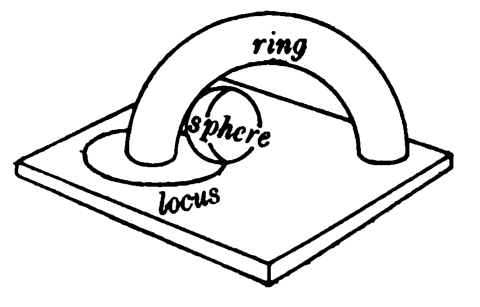
\includegraphics[width=0.6\linewidth]{pdf320-a.png}\end{center}

問題33。H. K. 図に示すように円環の半分が平面上に立ち、環と平面との両方に接する球が（球の直径 $d$ は、環の直截面の直径とそれに垂直な軸截面の直径との差に高々等しいものとし、これらの直径を $k$ および $l$ で表す）、環のまわりを回って平面上に軌跡を描く。この曲線の面積を求めることが要求される。

術。もし
\[
p=\frac{(k+d)(l+d)}{k^2+2kd},\qquad q=\frac{l+d}{k+d},
\]
\noindent および
\[
D_0=\frac{\pi}{4}p(l+d)\sqrt{k^2+2kd},\quad D_1=(p-q)D_0,\quad D_2=\frac{3.5}{2.4}pD_1,
\]

\scanpage{0321}{印刷頁 307}
\[
D_3 = \frac{5.11}{3.5}\text{\unclear{5 11}}\,p\Bigl(D_2 - \frac{1.3}{2.4}\text{\unclear{1 3}}\,qD_1\Bigr), \qquad
D_4 = \frac{7.9}{4.6}\text{\unclear{4 6}}\,p\Bigl(D_3 - \frac{2.4}{3.4}\,qD_2\Bigr),
\]
\[
D_5 = \frac{9.11}{5.7}\,p\Bigl(D_4 - \frac{3.5}{4.6}\,qD_3\Bigr), \ldots,
\]
求める面積は $D_0 + D_1 + D_2 + \cdots$ によって与えられる。

問題34。H. K. 二円 $A$ と $B$ があり、そのうち $A$ のほうが大きく、両者は互いに接し、その間に共通接線をもつとする。円 $A$ はその直線に沿って左へ転がり、一方、円 $B$ は $A$ との接触を保ちながら右へ回る。そして円 $B$ 上の、はじめ基線との接点と一致していた点は、円 $B$ に沿って右へ転がり、完全な回転を重ねて図に示すような軌跡を描く。円 $A$ と $B$ の直径および $MN = p$ の長さが与えられたとき、この曲線の面積を求めることが要求される。

\begin{center}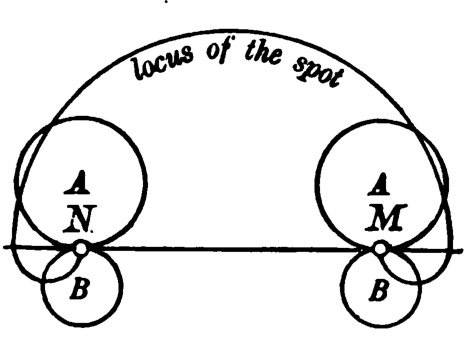
\includegraphics[width=0.6\linewidth]{pdf321-a.png}\end{center}

術。\quad 面積 $= \Bigl\{2B^2 + (A + B)^2\Bigr\}\,\frac{\pi}{4} + \frac{A}{2} \times p$。

問題35。H. K. これは問題33と同じであるが、ただ前の問題における環の半分の代りに環全体を取るという点だけが異なる。

\emph{Sampō Yenri Shiron}（これを S.Y.S. と略記する）の問題8。\footnote{この書は、高次の円理の諸問題について著者の先人たちが公にした解法を改訂したものであった。}図に示すように、円柱が斜めに通る楕円柱によって貫かれ、両者の軸は互いに直角をなすものと仮定されるとき、円柱の直径 $d$、楕円柱の底面の長径 $a$ と短径 $b$、および図中に $s_1$ と $s_2$ で示した長さが与えられたとして、貫かれた部分の体積を求めることが要求される。ここで $s_1$ と $s_2$ は、当該の母線に垂直に引かれたものである。

\begin{center}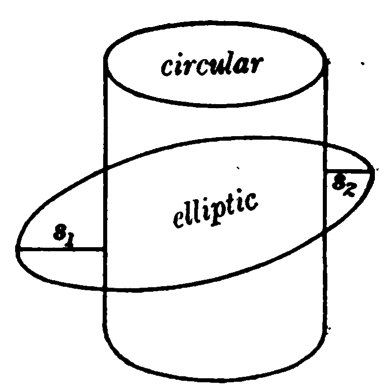
\includegraphics[width=0.6\linewidth]{pdf321-b.png}\end{center}

この問題は、Saitō Gigi の一八三四年の \emph{Yenri-kan} においてはじめて与えられたが、Hagiwara はその解法を誤りであるとして改訂した。

\scanpage{0322}{印刷頁 308 (top left)}
問題9. S. Y. S. 底面の直径が $d$ である円錐を図のように曲げて、軸 $h$ が直径 $d'$ の円の弧となるようにする。曲げの円の平面内にある母線\unclear{lines}に対応する曲線の長さを求めることが要求される。

\begin{center}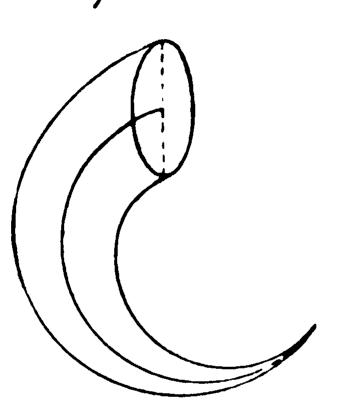
\includegraphics[width=0.6\linewidth]{pdf322-a.png}\end{center}

この問題は一八三六年の Kobayashi の \emph{Sampō Koren}\unclear{Korén} において初めて発表されたものであり、その解法では \emph{tetsu-jutsu} 展開が三度用いられた。その後、一八五五年の Kuwamoto の \emph{Sen-yen Kattsū} においても解かれた。しかし、どちらの解法もあまり簡単ではなかったので、Hagiwara は展開法を二度適用して、これを新たに解いた。

\begin{center}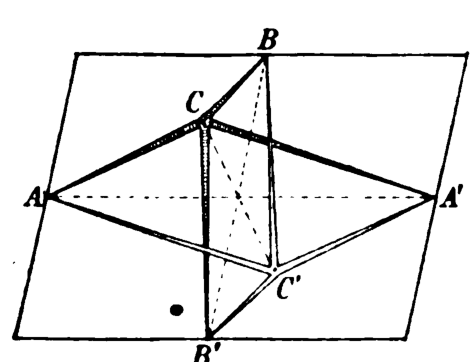
\includegraphics[width=0.6\linewidth]{pdf322-b.png}\end{center}

問題10. S. Y. S. \emph{choku-bishi}（一種のねじれ面である）の面積を、三つの軸 $AA' = a$,\quad $BB' = b$,\quad $CC' = c$ によって求めることが要求される。\emph{choku-bishi} とは、任意の二軸に平行な断面がすべて菱形となるような曲面、あるいは面から構成された図形である。

この問題について \emph{Sampō Koren} に与えられた解法は便利でなく、また Saitō の \emph{Yenri Shinshin} にある解法は正しくなかったので、Hagiwara は改訂した解法を得た。

問題31. S.Y.S. 楕円錐のうち円柱によって切り取られる部分の表面積を求めることが要求される。ただし両者の軸は直角に交わる。

Hagiwara の解法は、Murayama の \emph{Tsūki Sampō} にある解法を改訂したものであった。

\begin{center}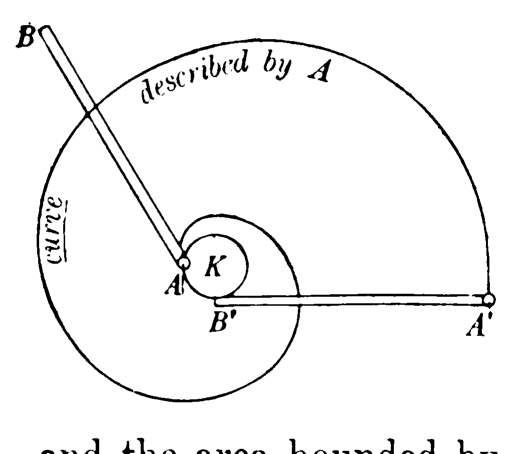
\includegraphics[width=0.6\linewidth]{pdf322-c.png}\end{center}

問題32. S. Y. S. 一端 $A$ において円 $K$ に接する棒 $AB = p$ が、円周に沿って滑ることなく回る。このとき端 $A$ は図に示すような曲線を描いて点 $A'$ で終わり、そのとき棒は $A'B'$ の位置をとって、もう一方の端\unclear{eud} $B$ が今度は円に接している。この曲線の長さ、および\unclear{aud}この曲線と円と棒の最終位置とによって囲まれる面積を求めることが要求される。

術。$s =$ 長さ、$a =$ 面積と書けば、次を得る。
\[
s = \frac{p^2}{K}, \quad \text{および} \quad a = s\times\frac{p}{3} - \frac{(p-K\pi)^3}{3K}, \quad \text{または} \quad a = s\times\frac{p}{3},
\]

\scanpage{0323}{印刷頁 309}
\noindent ここで面積の二つの式は、それぞれ $p - K\pi$ が正である場合と正でない場合に適用される。

この問題は以前に \emph{Tsūki Sampō} において考察されていたが、そこに与えられた術は、棒が円の周りを一回転を超えて回らない場合にのみ適用できるものであった。そこで Hagiwara は、これを一般に適用できるように改訂した。

問題34。S. Y. S. サイクロイドを、その最大の縦座標を軸として回転させて生じる曲面の面積を求めることが要求される。

術。面積 $= \left(2 - \dfrac{2}{3 \times \frac{\pi}{4}}\right)k^2$。ここで $k$ はサイクロイドの底辺の長さである。

これは \emph{Tsui-yen Hatsumō} に与えられた解法を改訂したものであった。

\emph{Yenri San-yō}（Y. S.）の問題4。図のように、高さの等しい二つの合同な円錐が直角に交わっている\unclear{intersecting/intersectiog}。その一方の軸が水平になるように、これを釣り合わせることが要求される。

\begin{center}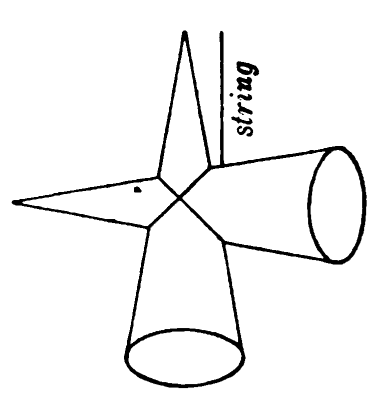
\includegraphics[width=0.3\linewidth]{pdf323-a.png}\quad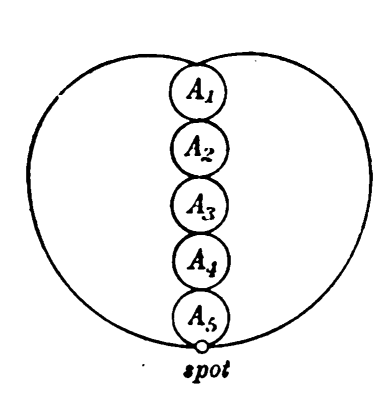
\includegraphics[width=0.3\linewidth]{pdf323-b.png}\end{center}

問題14。Y. S. 中心を一直線上にもち、順次に接する\unclear{touching/touchiug}、相等しい円（直径 $d$）が若干個（$n$ 個）描かれている。最後の円の円周上で、前述のこの直線の上に一点があるとする。そこで、第二の円が第一の円の周りを、第三の円が第二の円の周りを回り、以下同様にして、回転の向きがすべて同じであるとすれば、その点は一つの軌跡を描き、その形は上の図に示す通りであって、一回転の後に出発点に戻る。この卵形の面積を求めることが要求される。

術。面積 $= (2n - 1)n \times \frac{\pi}{4} \times d^2$。

問題15。偶数 $2n$ 個の円が、すべて共通の一点 $T$ で接するように描かれ、第一、第三、\dots\ の円は $T$ の一方の側にあり、残りの第二、第四、\dots\ の円はその他方の側にあって、同数からなる二つの円の列をなし、大きさの順に並び、第一と第二の円がそれぞれの列の最大のものであるとする。第 $2n$ の円の中心を $K$ とし、$K$ に一点があって、この点が属するものと仮定されるのは

\scanpage{0324}{印刷頁 310 (top left)}
\noindent $T$ を中心とし、その点を通るように描かれた円の円周。さて、第二の円は第一の円のまわりを回り、第三の円は第二の円のまわりを回り、以下同様であって、いずれも右へ回る。円 $T$ はその中心を第 $2n$ の円の上に置いたまま運ばれ、点あるいは斑点 $K$ は円 $T$ の上に載って運ばれる。回転の性質は、一回転を終えたのちに図全体がもとの形に戻るように考えられている。$K$ の描く軌跡は明らかに閉曲線であり、$T$ の軌跡もまた同様である。この二つの軌跡によって作られる環状部の面積を求めることが要求される。

\begin{center}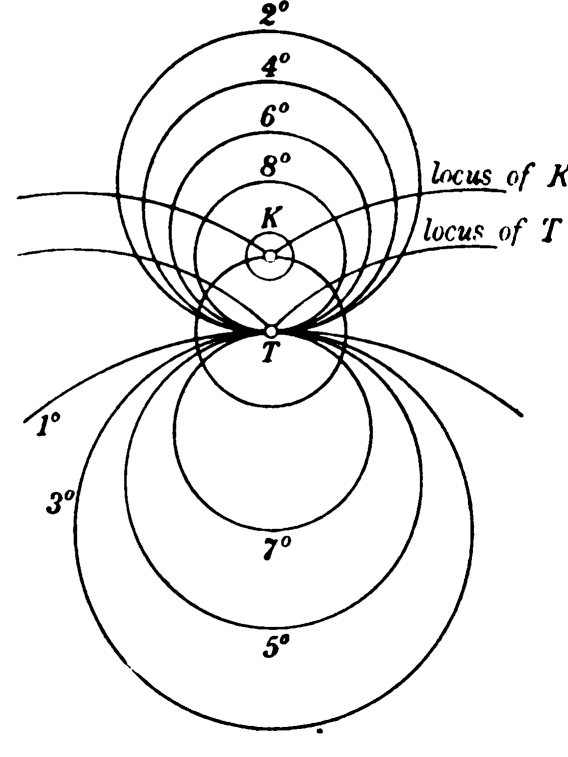
\includegraphics[width=0.6\linewidth]{pdf324-a.png}\end{center}

術。円 $T$ の直径を $d$ とすれば、求める面積は $d^2\times\frac{\pi}{4}\times(2n+1)$ となる。

問題20。Y. S. 図に示すように四つの等しい円錐によって作られる図形の体積を、円錐の高さと直径、および図形の長さと幅によって求めることが要求される。

\begin{center}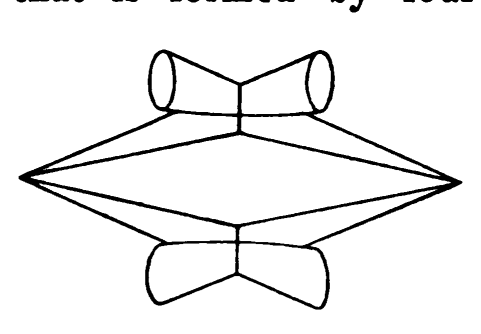
\includegraphics[width=0.6\linewidth]{pdf324-b.png}\end{center}

また、この問題と同様の仕方で多数の等しい円錐から構成される図形の体積および側面積を求める問題もある。

問題25。Y. S. 円柱を回転楕円体と斜めに交わらせ、後者が前者の一つの母線に内側から接するようにして作られた図形がある。この立体を、前述の母線の反対側にある母線と一致する糸によって吊るして釣り合わせるとき、円柱の高さはどれだけになるか。ここで、回転楕円体の長径と短径（前者が回転軸である）、吊り線に垂直に引いた最長の矢\footnote{この語句で意味するのは、円柱の反対側にある基準線から回転楕円体上の点までの、最大の垂直距離である。}、および円柱の直径は既知であると仮定する。

問題30。Y. S. この直径の一端に接する円柱によって穴を貫かれた、長径を軸とする回転楕円体が、平らな板の上に置かれている。

\scanpage{0325}{印刷頁 311}
\noindent これを、その板との接点を通り、かつ軸を含む鉛直平面に垂直な鉛直平面で切る。楕円体の二つの直径と円柱の直径が与えられたとき、切り取られた部分の体積を求めることが要求される。

5. Hagiwara が考察した問題のうちいくつかの解法は、次の諸章で与えられる。彼は解法の規則において時に対数級数を用いたが、これは友人 Okamoto Norifumi の示唆によって、彼が西洋の学問から借りたものであった。

伝えるところによれば、全国に \emph{Yenri San-yō} のすべての問題の結果を検証しうる者は一人もおらず、Hagiwara の自負はこの上なく満たされたが、ただ一人の例外が Ōmura Isshū であって、彼はその問題のいくつかを解くことができたという。Ōmura はヨーロッパの数学にいくらか通じていたが、この分野における彼の知識はきわめて限られたものであった。

Hagiwara は、研究において他人がまさっていることを認める気になることのめったにない人物であった。しかし彼は、自分より数歳年長であったこの Ōmura の才能には感服せずにはいられなかった。Hōdōji Wajūrō、Suzuki Yen、Takaku Kenjirō、Iwata Sempei（Iwata Kōsan の名でよりよく知られる。Kōsan は彼の雅号である）その他の人々は、彼が敬意を示した人々の中に入っていた。彼は、Takuma\unclear{Takuma's / Takumá's / Takumā's} の流派の数学者で、おそらく今なお存命である Sonobe Keizō を高く評価していた。

Hagiwara の未刊の著作の中では、畳み、すなわち積分の目的のために彼が作成または改訂した表を挙げることができる。これらの表については、われわれは研究を遂行する好機を得たいと望んでいる。Hagiwara のその他の著作は、われわれの今後の研究の主題をなすに足る深い興味に満ちたものであろうと期待している。

\begin{center}
第45章。\\[1mm]
平面上に立つ円環体のまわりを転がる球が描く曲線の面積に関する HAGIWARA の公式。
\end{center}
\phantomsection\addcontentsline{toc}{subsection}{第45章　平面上に立つ円環体のまわりを転がる球が描く曲線の面積に関する HAGIWARA の公式}

一八六二年に刊行された Hagiwara Teisuke の \emph{Sampō Hōyen-kan} には、次のような問題が収められている。「平らな台の上に垂直に立つ円環体がある。その底部で環に接する球が、一周ののち最初の位置に戻るまで、環のまわりを転がる。球が平面上に描く軌跡は、一つの

\scanpage{0326}{印刷頁 312}
特殊な形である。環の直径、その断面の直径、および球の直径（最大のときには環の直径に等しい）が与えられたとき、軌跡の面積を求めることが要求される。」

\begin{center}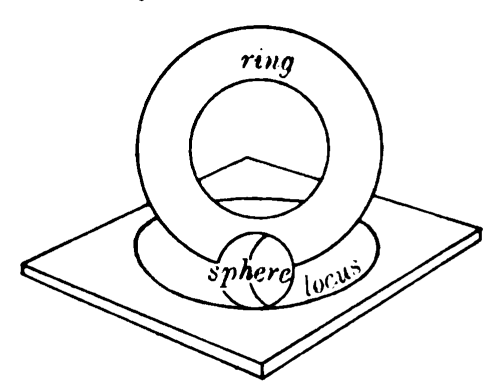
\includegraphics[width=0.6\linewidth]{pdf326-a.png}\end{center}

環の直径を $a$、球の直径を $b$、環の断面の直径を $c$ とする。このとき、Hagiwara の解法の術は次のように表すことができる。
\[
(\text{面積}) = ab\pi(D_0 - D_1 - D_2 - D_3 - \cdots),
\]
ここで $k = \dfrac{a}{b+c}$ および $t = \dfrac{b}{a}$ と書き、また
\[
A = \frac{1}{\sqrt{k}}, \quad B = \frac{3}{1\,.\,2}Ak, \quad C = \frac{1\,.\,5}{3\,.\,4}Bk, \quad D = \frac{3\,.\,7}{5\,.\,6}Ck, \quad E = \frac{5\,.\,9}{7\,.\,8}Dk, \ldots;
\]
\[
\alpha = \frac{1}{4}t, \quad \beta = \frac{3}{6}\alpha t, \quad \gamma = \frac{5}{8}\beta t, \quad \delta = \frac{7}{10}\gamma t, \ldots;
\]
と書けば、量 $D_0$ および $D_1$, $D_2$, .\,. は次の形をもつ。
\begin{align*}
&D_0 = A, \quad D_1 = \alpha\Bigl(B + \tfrac{1}{2}A\Bigr), \quad D_2 = \beta\Bigl[C - \tfrac{1}{2}\Bigl(B - \tfrac{1}{4}A\Bigr)\Bigr],\\
&D_3 = \gamma\Bigl[D - \tfrac{1}{2}\Bigl\{C + \tfrac{1}{4}\Bigl(B - \tfrac{3}{6}A\Bigr)\Bigr\}\Bigr],\\
&D_4 = \delta\Bigl[E - \tfrac{1}{2}\Bigl\{D + \tfrac{1}{4}\,\Bigl|\overline{C + \tfrac{3}{6}\Bigl(B - \tfrac{5}{8}A\Bigr)}\Bigr\}\Bigr], \ldots
\end{align*}

Hagiwara の著作では、この術は何の説明もなく公にされた。ここでは、Ōmura Isshū が自身の写本の一つにおいて試みたこの問題の解析を補うことにする。

Ōmura はまず、ここに再現する通りの図を与える。

\begin{center}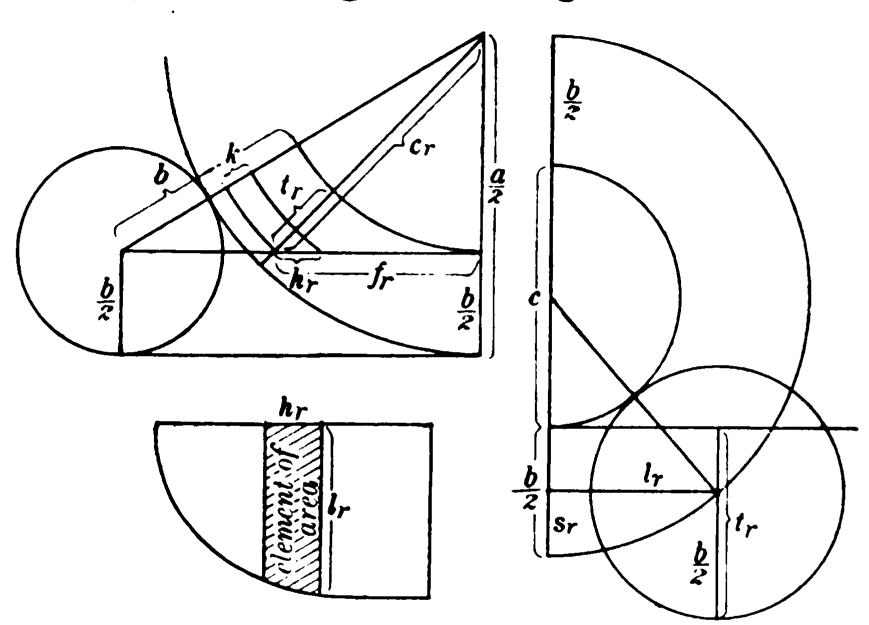
\includegraphics[width=0.6\linewidth]{pdf326-b.png}\end{center}

ここでは図の作り方は説明されておらず、また容易には理解しがたい点もいくつかあるが、われわれは試みられた解析をたどるだけにとどめる。図の性質は、種々の長さを表す式から明らかになるであろう。すなわち、$n$ を分割の数とすれば、次を得る。
\[
k = \frac{b}{n}; \quad t_r = b \times \frac{r}{n} = bi,\ \text{とおく}; \quad s_r = b - t_r = (1 - i)b;
\]
\[
l_r^2 = (b + c)s_r - s_r^2 = (1 - i)b(b + c)\{1 - \varrho(1 - i)\},
\]

\scanpage{0327}{印刷頁 313}
\noindent ここで $\varrho = b/(b + c)$ である。あるいは展開すれば、
\begin{multline*}
l_r = \sqrt{1 - i}\,\sqrt{b}\,\sqrt{b + c}\,\Bigl\{1 - \tfrac{1}{2}(1 - i)\,\varrho - \tfrac{1}{8}(1 - i)^2\varrho^2 - \tfrac{3}{48}(1 - i)^3\varrho^3\\
{} - \tfrac{15}{384}(1 - i)^4\varrho^4 - \cdots\Bigr\};
\end{multline*}
\[
c_r = t_r + \frac{a + b}{2} = ib + \frac{a - b}{2};
\]
\[
f_r^2 = c_r^2 - \left(\frac{a - b}{2}\right)^2 = i^2b^2 - ib^2 + iab = iab\{1 - \Phi(1 - i)\},
\]
ここで $\Phi = b/a$ であり、これから次を得る。
\begin{multline*}
\frac{1}{f_r} = \frac{1}{\sqrt{abi}}\Bigl\{1 + \tfrac{1}{2}\Phi(1 - i) + \tfrac{3}{8}\Phi^2(1 - i)^2 + \tfrac{15}{48}\Phi^3(1 - i)^3\\
{} + \tfrac{105}{384}\Phi^4(1 - i)^4 + \cdots\Bigr\};
\end{multline*}
\[
\frac{h_r}{k} = \frac{c_r}{f_p} = \frac{1}{f_r}\,a\Bigl\{\tfrac{1}{2} + \tfrac{1}{2}\Phi - \Phi(1 - i)\Bigr\},
\]
\begin{multline*}
\therefore\ \frac{h_r\sqrt{abi}}{k} = a\Bigl\{\tfrac{1}{2} - \tfrac{3}{4}\Phi(1 - i) - \tfrac{5}{16}\Phi^2(1 - i)^2 - \tfrac{21}{96}\Phi^3(1 - i)^3\\
\shoveright{{} - \tfrac{135}{2.384}\Phi^4(1 - i)^4 - \cdots\Bigr\}}\\
{} + a\Phi\Bigl\{\tfrac{1}{2} + \tfrac{1}{4}\Phi(1 - i) + \tfrac{3}{16}\Phi^2(1 - i)^2 + \tfrac{15}{96}\Phi^3(1 - i)^3\\
{} + \tfrac{105}{2.384}\Phi^4(1 - i)^4 + \cdots\Bigr\};
\end{multline*}
また面積要素 $= A_r = h_r\,l_r$ と書けば、次を得る。
\[
\begin{array}{@{}l@{\;}l@{\;}l@{\;}l@{\;}l@{}}
\multicolumn{5}{c}{\dfrac{A_r}{k\sqrt{a\,(b + c)}}}\\[4mm]
= \dfrac{\sqrt{1 - i}}{2\sqrt{i}}
 & {} - \dfrac{3\sqrt{1 - i}\,(1 - i)}{4\sqrt{i}}\,\Phi
 & {} - \dfrac{5\sqrt{1 - i}\,(1 - i)^2}{16\sqrt{i}}\,\Phi^2
 & {} - \dfrac{21\sqrt{1 - i}\,(1 - i)^3}{96\sqrt{i}}\,\Phi^3
 & {} - \cdots\\[4mm]
+ \dfrac{\varrho}{2}\biggl(
 & {} - \dfrac{\sqrt{1 - i}\,(1 - i)}{2\sqrt{i}}
 & {} + \dfrac{3\sqrt{1 - i}\,(1 - i)^2}{4\sqrt{i}}\,\Phi
 & {} + \dfrac{5\sqrt{1 - i}\,(1 - i)^3}{16\sqrt{i}}\,\Phi^2
 & {} + \cdots\biggr)\\[4mm]
+ \dfrac{\varrho^2}{8}\biggl(
 &
 & {} - \dfrac{\sqrt{1 - i}\,(1 - i)^2}{2\sqrt{i}}
 & {} + \dfrac{3\sqrt{1 - i}\,(1 - i)^3}{4\sqrt{i}}\,\Phi
 & {} + \cdots\biggr)\\[4mm]
+ \dfrac{3\varrho^3}{48}\biggl(
 &
 &
 & {} - \dfrac{\sqrt{1 - i}\,(1 - i)^3}{2\sqrt{i}}
 & {} + \cdots\biggr)\\[4mm]
+ & \multicolumn{4}{l}{\dotfill}
\end{array}
\]

\scanpage{0328}{印刷頁 314 (top left)}
\[
\begin{array}{@{}r@{\,}l@{\;}l@{\;}l@{\;}l@{}}
+ & \dfrac{\sqrt{1-i}}{2\sqrt{i}}\,\varPhi
  & {}+\dfrac{\sqrt{1-i}\,(1-i)}{4\sqrt{i}}\,\varPhi^{2}
  & {}+\dfrac{3\sqrt{1-i}\,(1-i)^{2}}{16\sqrt{i}}
  & {}+\cdots\\[4mm]
+ & \dfrac{\varrho}{2}\Biggl(
  & {}-\dfrac{\sqrt{1-i}\,(1-i)}{4\sqrt{i}}\,\varPhi
  & {}-\dfrac{\sqrt{1-i}\,(1-i)^{2}}{4\sqrt{i}}\,\varPhi^{2}
  & {}-\cdots\Biggr)\\[4mm]
+ & \dfrac{\varrho^{2}}{8}\Biggl(
  &
  & {}-\dfrac{\sqrt{1-i}\,(1-i)^{2}}{2\sqrt{i}}\,\varPhi
  & {}-\cdots\Biggr)\\[4mm]
+ & \multicolumn{4}{l}{.\quad.\quad.\quad.\quad.\quad.\quad.\quad.\quad.\quad.\quad.\quad.\quad.\quad.\quad.\quad.\quad.\quad.\quad.}
\end{array}
\]

この式を畳む、すなわち $i=\frac{1}{n},\frac{2}{n},\cdots,\frac{n}{n}$ について総和をとり、極限 $n=\infty$ に移るならば、
\[
\begin{array}{@{}l@{}}
\begin{array}{@{}r@{\,}l@{\;}l@{\;}l@{\;}l@{\;}l@{}}
\dfrac{\text{(面積)}}{\pi b\sqrt{a}\cdot\sqrt{b+c}}={}
  & \dfrac{2}{2}
  & {}-\dfrac{3\cdot3\varPhi}{2.4}
  & {}-\dfrac{5.15\varPhi^{2}}{2.6.16}
  & {}-\dfrac{21.105\varPhi^{3}}{2.8.6.96}
  & {}-\cdots\\[3mm]
+ & \dfrac{\varrho}{2}\biggl(
  & {}-\dfrac{3}{2.2}
  & {}+\dfrac{3.15\varPhi}{2{,}6.4}\text{\unclear{$2,6.4$ or $2.6.4$}}
  & {}+\dfrac{5.105\varPhi^{2}}{2.8.6.16}
  & {}+\cdots\biggr)\\[3mm]
+ & \dfrac{\varrho^{2}}{8}\biggl(
  &
  & {}-\dfrac{15}{2.6.2}
  & {}+\dfrac{3.105\varPhi}{2.8.6.4}
  & {}+\cdots\biggr)\\[3mm]
+ & \dfrac{3\varrho^{3}}{48}\biggl(
  &
  &
  & {}-\dfrac{105}{2.8.6.2}
  & {}+\cdots\biggr)+\cdots
\end{array}\\[3mm]
\qquad\quad
\begin{array}{@{}r@{\,}l@{\;}l@{\;}l@{\;}l@{\;}l@{}}
+ & \dfrac{2\varPhi}{2}
  & {}+\dfrac{3\varPhi^{2}}{4}
  & {}+\dfrac{3.15\varPhi^{3}}{2.6.16}
  & {}+\dfrac{15.105\varPhi^{4}}{2.6.8.96}
  & {}+\cdots\\[3mm]
+ & \dfrac{\varrho}{2}\biggl(
  & {}-\dfrac{3\varPhi}{2.2}
  & {}-\dfrac{15\varPhi^{2}}{2.6.4}
  & {}-\dfrac{3.105\varPhi^{3}}{2.8.6.16}
  & {}-\cdots\biggr)\\[3mm]
+ & \dfrac{\varrho^{2}}{8}\biggl(
  &
  & {}-\dfrac{15\varPhi}{2.6.2}
  & {}-\dfrac{105\varPhi^{2}}{2.8.6.4}
  & {}-\cdots\biggr)\\[3mm]
+ & \dfrac{3\varrho^{3}}{48}\biggl(
  &
  &
  & {}-\dfrac{105\varPhi}{2.8.6.2}
  & {}-\cdots\biggr)+\cdots
\end{array}\\[3mm]
\begin{array}{@{}r@{\,}l@{\;}l@{\;}l@{\;}l@{\;}l@{\;}l@{}}
={} & \dfrac{2}{2}
  & {}-\dfrac{\varPhi}{8}
  & {}-\dfrac{3\varPhi^{2}}{2.6.16}
  & {}-\dfrac{3.15\varPhi^{3}}{2.8.6.96}
  & {}-\dfrac{15.105\varPhi^{4}}{2.10.8.6.2.384}
  & {}-\cdots\\[3mm]
  &
  & {}-\dfrac{3\varrho}{8}
  & {}+\dfrac{9\varPhi\varrho}{2.48}
  & {}+\dfrac{45\varPhi^{2}\varrho}{8.384}
  & {}+\dfrac{945\varPhi^{3}\varrho}{48.3840}
  & {}+\cdots\\[3mm]
  &
  &
  & {}-\dfrac{15\varrho^{2}}{192}
  & {}+\dfrac{75\varPhi\varrho^{2}}{8.384}
  & {}+\dfrac{105.5\varPhi^{2}\varrho^{2}}{48.3840}
  & {}+\cdots\\[3mm]
  &
  &
  &
  & {}-\dfrac{105.3\varrho^{3}}{48.192}
  & {}+\dfrac{105.21\varPhi\varrho^{3}}{48.3840}
  & {}+\cdots\\[3mm]
  &
  &
  &
  &
  & {}-\dfrac{945.15\varrho^{4}}{5.164^{2}}\text{\unclear{$164^{2}$ or $384^{2}$}}
  & {}+\cdots\\[2mm]
  &
  &
  &
  &
  & \multicolumn{2}{l}{.\quad.\quad.\quad.\quad.\quad.\quad.}
\end{array}
\end{array}
\]
を得る。

Hagiwara の法則は、この二重級数から導かれる。

\scanpage{0329}{印刷頁 315 (top right)}
\begin{center}
第46章。\\[1mm]
捩れ面。
\end{center}
\phantomsection\addcontentsline{toc}{subsection}{第46章　捩れ面}

1. $ABCD$ を捩れ四辺形とする。対辺 $AB$ と $CD$ をそれぞれ同数の等しい部分に分け、対応する分点を直線で結ぶ。もう一組の対辺 $AD$ と $BC$ についても同じ作図を行う。その結果は一種の網である。二組の分割数を限りなく増すと、捩れ面が得られる。このような面に関連するいくつかの図形の計算が、一九世紀の日本の数学者たちによって試みられた。

この面に関する問題に最初に出会うのは、一八三六年に刊行された Kobayashi の \emph{Sampō Koren} においてである。それは、のちに Hagiwara が研究したのと同じ \emph{choku-bishi} の問題である。互いに直角をなし、それぞれの中点で交わる三本の軸をとり、そのうちの二本を一組の中線とする矩形を作れば、矩形の辺の線分と、軸の端点を結ぶ線のうち矩形と同一平面上にあるものを除いたものとによって、八つの捩れ四辺形が形成される。これらの捩れ四辺形を底とする捩れ面によって囲まれる図形が、いわゆる \emph{choku-bishi} である。

この図形の全表面積を求める問題についての Kobayashi の結果は、Shinano 国 Uyeda のある寺の前に掲げられた形で示された。

一八四〇年の Saitō の \emph{Yenri Shinshin} では、\emph{choku-bishi} の半分である図形の側面積を求める問題が考察された。

Fujioka Yūtei もまた、一八四五年の著書 \emph{Sampō Yenri-tsū} においてこの面を考察した。このほかにも、捩れ面に関する問題が見られる刊本がある。しかしこれらの刊行物はいずれも計算の結果を載せているにすぎず、同時に解析をも考察したものは一つもない。したがって、Kobayashi およびその他の初期の著者たちが従った取扱い方については、われわれは何も知らない。それゆえわれわれは、Hōdōji Wajūrō と Hagiwara Teisuke が試みた手順を述べなければならない。

2. Hōdōji の書いた写本に、「\emph{Sampō Koren} 第十二問の解析」と題するものがある。ここではその書の結果を示す。まず彼は次のように考える。$ABCD$ を求積すべき捩れ面とする。一つの

\scanpage{0330}{印刷頁 316}
図に示すような作図をする。ここで $DCB'A'$ は矩形であり、$AA'$ と $BB'$ はその平面に垂直、$PQ \parallel P_1Q_1 \parallel AB$, $PP' \parallel P_1P_1' \parallel AA'$,
\begin{center}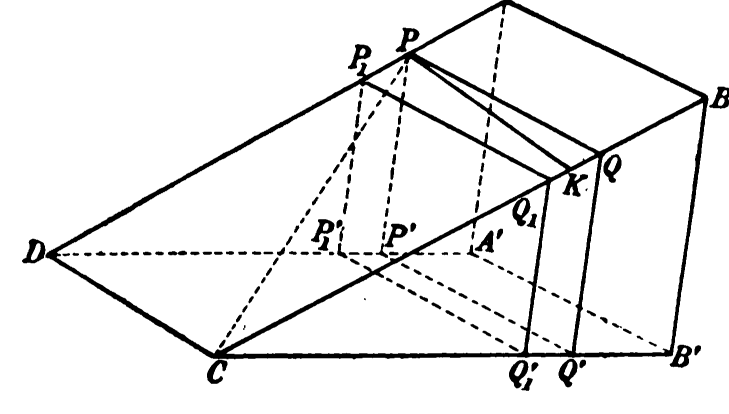
\includegraphics[width=0.6\linewidth]{pdf330-a.png}\end{center}
$QQ' \parallel Q_1Q_1' \parallel BB'$, $P'Q' \parallel P_1'Q_1' \parallel A'B'$ である。$PQQ'P'$, $P_1Q_1Q_1'P_1'$ を、ねじれ面を $n$ 個の部分に分けるように等間隔に作った平行平面のうちの相続く二平面とする。このとき $Q'Q_1' = \frac{1}{n} \cdot B'C$ および $Q'C = \frac{r}{n} \cdot B'C$ と書くことができる。$PC$ を結び、$P$ から $BC$ に直角に $PK$ を引く。まず $PK.QQ_1$ を面積の要素 $(A_r)$ とする。こうして\footnote{$KC$ の式の導出は与えられていない。}
\[
PC^2 = CQ'^2 + P'Q'^2 + PP'^2, \quad KC = \frac{r}{n}\,\frac{1}{BC}\,(B'C^2 + AA'.BB'),
\]
\[
\therefore PK^2 = PC^2 - KC^2 = CD^2 + (AA' - BB')^2 CB'^2 \cdot \frac{1}{BC^2} \cdot \frac{r^2}{n^2},
\]
を得る。これを仮に $= CD^2 \left\{1 + \frac{r^2}{n^2}\alpha\right\}$ と書く。したがって
\[
\begin{aligned}
A_r = PK.QQ_1 = BC.CD \cdot \frac{1}{n}\biggl\{1 + \frac{1}{2}\alpha\left(\frac{r}{n}\right)^2 - \frac{1}{8}\alpha^2\left(\frac{r}{n}\right)^4 + \frac{3}{48}\alpha^3\left(\frac{r}{n}\right)^6 &\\
- \frac{15}{384}\alpha^4\left(\frac{r}{n}\right)^8 + \cdots\biggr\}&,
\end{aligned}
\]
となり、畳むという操作、すなわち項別積分によって
\[
\begin{aligned}
\text{(面積)} &= BC.CD\left\{1 + \frac{1}{3\,.\,2}\alpha - \frac{1}{5\,.\,8}\alpha^2 + \frac{3}{7\,.\,48}\alpha^3 - \frac{15}{9\,.\,384}\alpha^4 + \cdots\right\}\\
&= BC.CD\left\{1 + \frac{1}{2\,.\,3}\alpha - \frac{1\,.\,3}{4\,.\,5}\alpha D_1 + \frac{3\,.\,5}{6\,.\,7}\alpha D_2 - \frac{5\,.\,7}{8\,.\,9}\alpha D_3 + \cdots\right\},
\end{aligned}
\]
を得る。ここで $D_1$, $D_2, \ldots$ は、通例どおり順次の差を表す。

しかし、上の手続きが正当であるならば、$Q$ から $AD$ へ垂線 $QK'$ を引き、$QK'.PP_1$ を面積の要素とすることもまた正当でなければならない。この場合には、計算\footnote{これは前の場合と同じく Hōdōji によって与えられている。}によって次の公式が得られる。
\[
\text{(面積)} = AD.CD\left\{1 + \frac{1}{2\,.\,3}\alpha' - \frac{1\,.\,3}{4\,.\,5}\alpha' D_1 + \frac{3\,.\,5}{6\,.\,7}\alpha' D_2 - \frac{5\,.\,7}{8\,.\,9}\alpha' D_3 + \cdots\right\},
\]
ここで $\alpha' = (AA' - BB')B'C^2/CD^2.AD^2$ であり、これは前の $\alpha = (AA' - BB')^2 B'C^2/CD^2.BC^2$ に代わるものである。

問題で考えている長さにいくつかの数値を与えれば、上の二つの公式はいくらか

\scanpage{0331}{印刷頁 317}
\noindent 問題の面積に対して異なる値を与え、\footnote{結論を除いては、数値計算もその結果も与えられていない。}これは両公式がともに正当でないことの証拠である。

\begin{center}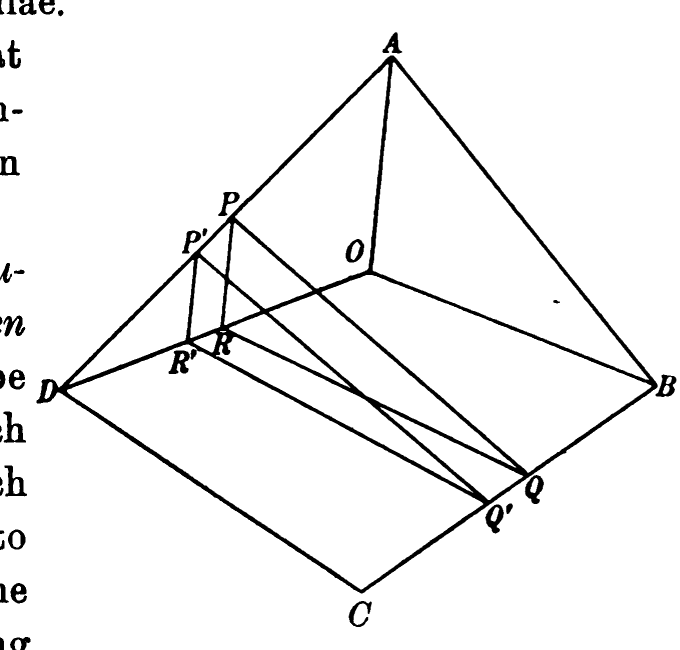
\includegraphics[width=0.6\linewidth]{pdf331-a.png}\end{center}

3. こうして Hōdōji は、上の取扱い方は正しくないと結論するが、そこでさらに進んで考察を加える。

\emph{Sampō Koren} で考察されている \emph{chokubishi} の八分の一の部分は、添付の図のような形をしており、$ABO$ に平行に等間隔に引いた平面によって切り取られる $PQQ'P'$ のような要素部分から成るものと考えることができる。これらの部分の一つを、上で得た二公式のうち第一のものに従って取り扱う。このとき
\[
QQ' = \frac{1}{n}\cdot OD, \quad PR = \frac{r}{n}\,OA, \quad P'R' = \left(\frac{r}{n} - \frac{1}{n}\right) OA,
\]
\[
PQ^2 = OB^2 + \left(\frac{r}{n}\right)^2 OA^2 = OB^2\,.\,k,
\]
である。ここで次のように書く。
\[
t = \frac{OA^2}{OB^2}, \quad k = 1 + \left(\frac{r}{n}\right)^2 t;\ \text{また}\ s = \frac{OA^2}{OD^2}.
\]

そこで前述の公式を適用し、その際 $2\,.\,OB = a$, $2\,.\,OD = b$, $2\,.\,OA = c$ と書き、$PQQ'P'$ の四倍を面積要素 $(A_r)$ とすれば、次を得る。
\[
A_r = ab\,\frac{1}{n}\left\{\sqrt{k} + \frac{1}{3.2}\,\frac{s}{\sqrt{k}} - \frac{1}{5.8}\,\frac{s^2}{k\sqrt{k}} + \frac{3}{7\,.\,48}\,\frac{s^3}{k^2\sqrt{k}} - \frac{15}{9.384}\,\frac{s^4}{k^3\sqrt{k}} + \cdots\right\}.
\]

括弧内の各項を順に $D_0$, $D_1$, $D_2, \ldots$ で表し、$\sqrt{k}$ を展開すれば、次を得る。
\[
\begin{array}{@{}l@{\;}c@{\;}l@{}}
D_0 = & & \left\{\phantom{-}1 + \frac{1}{2}\,t\left(\frac{r}{n}\right)^{2} - \frac{1}{8}\,t^{2}\left(\frac{r}{n}\right)^{4} + \frac{3}{48}\,t^{3}\left(\frac{r}{n}\right)^{6} - \frac{15}{384}\,t^{4}\left(\frac{r}{n}\right)^{8} + \cdots\right\},\\[3mm]
D_1 = & \frac{s}{3\,.\,2} & \left\{\phantom{-}1 - \frac{1}{2}\,t\left(\frac{r}{n}\right)^{2} + \frac{3}{8}\,t^{2}\left(\frac{r}{n}\right)^{4} - \frac{15}{48}\,t^{3}\left(\frac{r}{n}\right)^{6} + \frac{105}{384}\,t^{4}\left(\frac{r}{n}\right)^{8} - \cdots\right\}.\\[3mm]
D_2 = & \frac{s^{2}}{5\,.\,8} & \left\{-1 + \frac{3}{2}\,t\left(\frac{r}{n}\right)^{2} - \frac{15}{8}\,t^{2}\left(\frac{r}{n}\right)^{4} + \frac{105}{48}\,t^{3}\left(\frac{r}{n}\right)^{6} - \frac{945}{384}\,t^{4}\left(\frac{r}{n}\right)^{8} + \cdots\right\},\\[3mm]
D_3 = & \frac{3\,s^{3}}{7\,.\,48} & \left\{\phantom{-}1 - \frac{5}{2}\,t\left(\frac{r}{n}\right)^{2} + \frac{35}{8}\,t^{2}\left(\frac{r}{n}\right)^{4} - \frac{315}{48}\,t^{3}\left(\frac{r}{n}\right)^{6} + \frac{3465}{384}\,t^{4}\left(\frac{r}{n}\right)^{8} - \cdots\right\},\\[3mm]
D_4 = & \frac{15\,s^{4}}{9.384} & \left\{-1 + \frac{7}{2}\,t\left(\frac{r}{n}\right)^{2} - \frac{63}{8}\,t^{2}\left(\frac{r}{n}\right)^{4} + \frac{693}{48}\,t^{3}\left(\frac{r}{n}\right)^{6} - \frac{9009}{384}\,t^{4}\left(\frac{r}{n}\right)^{8} + \cdots\right\},
\end{array}
\]
\noindent\dotfill

\scanpage{0332}{印刷頁 318}
次に、折り畳みの演算を行ってその結果を二倍すると、\emph{choku-bishi} の全面積として式 $2ab(D_0+D_1+D_2+\cdots)$ を得る。ここで
\[
\begin{array}{r@{}c@{\,}l}
D_0={} & & \left(\phantom{-}1+\frac{1}{3.2}t-\frac{1}{5.8}t^2+\frac{3}{7.48}t^3-\frac{15}{9.384}t^4+\cdots\right),\\[3mm]
D_1={} & \frac{s}{3.2} & \left(\phantom{-}1-\frac{1}{3.2}t+\frac{3}{5.8}t^2-\frac{15}{7.48}t^3+\frac{105}{9.384}t^4-\cdots\right),\\[3mm]
D_2={} & \frac{s^2}{5.8} & \left(-1+\frac{3}{3.2}t-\frac{15}{5.8}t^2+\frac{105}{7.48}t^3-\frac{945}{9.384}t^4+\cdots\right),\\[3mm]
D_3={} & \frac{3s^3}{7.48} & \left(+1-\frac{5}{3.2}t+\frac{35}{5.8}t^2-\frac{315}{7.48}t^3+\frac{3465}{9.384}t^4-\cdots\right),\\[3mm]
D_4={} & \frac{15s^4}{9.384} & \left(-1+\frac{7}{3.2}t-\frac{63}{5.8}t^2+\frac{693}{7.48}t^3-\frac{9009}{9.384}t^4+\cdots\right),\\[3mm]
\multicolumn{3}{l}{.\quad.\quad.\quad.\quad.\quad.\quad.\quad.\quad.\quad.\quad.\quad.\quad.\quad.\quad.\quad.\quad.\quad.\quad.\quad.}
\end{array}
\]
である。

\emph{chokubishi} の面積を表すこの式を変形するために、Hōdōji は次のように進める。$p=1+t$ と書けば、実際に計算してみることによって、$D_1$, $D_2,\ldots$ が次のように書き直せることがわかるであろう。
\[
\begin{aligned}
&D_1=\frac{s}{3.2}\bigl(2D_0-\sqrt{p}\bigr),\qquad D_2=-\frac{s^2}{5.8\sqrt{p}},\qquad D_3=\frac{s^3}{7.48}\left(\frac{2}{\sqrt{p}}+\frac{1}{p\sqrt{p}}\right),\\
&D_4=\frac{3s^4}{9.384}\left\{\frac{1}{3}\left(-\frac{8}{\sqrt{p}}-\frac{4}{p\sqrt{p}}\right)-\frac{1}{p^2\sqrt{p}}\right\},\\
&D_5=\frac{15s^5}{11.3840}\left[\frac{1}{5}\left\{\frac{1}{3}\left(\frac{48}{\sqrt{p}}+\frac{24}{p\sqrt{p}}\right)+\frac{6}{p^2\sqrt{p}}\right\}+\frac{1}{p^2\sqrt{p}}\text{\unclear{$p^2$ or $p^3$}}\right],\ \ldots
\end{aligned}
\]

ここで
\begin{multline*}
A_1=\frac{s\sqrt{p}}{2},\qquad A_2=\frac{1}{4}A_1\frac{s}{p},\qquad A_3=\frac{1}{6}A_2\frac{s}{p},\qquad A_4=\frac{3}{8}A_3\frac{s}{p},\\
A_5=\frac{5}{10}A_4\frac{s}{p},\ \ldots;
\end{multline*}
\[
B=1+\frac{s}{3},\quad B_1=\frac{Bt}{2},\quad B_2=\frac{B_1t}{4},\quad B_3=\frac{3B_2t}{6},\quad B_4=\frac{5B_3t}{8},\ldots,
\]
と書けば、因数 $2ab$ を除いた面積の式は、$D_0$ をその展開形で表すことにすると、次のように書くことができる。
\begin{gather*}
\begin{array}{r@{\;}c@{\;}c@{\;}c@{\;}c@{\;}c@{\;}l}
B & {}+\dfrac{B_1}{3} & {}-\dfrac{B_2}{5} & {}+\dfrac{B_3}{7} & {}-\dfrac{B_4}{9} & {}+\dfrac{B_5}{11} & {}-\cdots\\[3mm]
 & {}-\dfrac{A_1}{3} & {}-\dfrac{A_2}{5} & {}+\dfrac{sA_2}{7.3} & {}-\dfrac{s^2A_2}{9.6} & {}+\dfrac{s^3A_2}{11.10} & {}-\cdots\\[3mm]
 & & & {}+\dfrac{A_3}{7} & {}-\dfrac{sA_3}{9.2} & {}+\dfrac{6s^2A_3}{11.2.10} & {}-\cdots\\[3mm]
 & & & & {}-\dfrac{A_4}{9} & {}+\dfrac{6sA_4}{11.10} & {}-\cdots\\[3mm]
 & & & & & {}+\dfrac{A_5}{11} & {}-\cdots\\[3mm]
 & & & & & & {}-\cdots
\end{array}\\[3mm]
{}=B+\frac{B_1-A_1}{3}-\frac{B_2+A_2}{5}+\frac{B_3+P_1}{7}-\frac{B_4+P_2}{9}-\frac{B_5+P_3}{11}-\cdots
\end{gather*}

\scanpage{0333}{印刷頁 319}
\noindent ここでは、逐次の諸項を縦の列に従って合計し、略記 $P_1$, $P_2$, \dots\ を用いている。

上式は、Kobayashi が一八三六年の \emph{Sampō Koren} において与えた公式そのものである。しかし Hōdōji が主張するように、彼の解析は誤った公式に基づいていた。それゆえ彼は、こうして得られた公式もそれ自体誤りであると結論する。

4. しかし Hagiwara Teisuke は考えを異にした。彼は幾度もその結果について Hōdōji と論じ合い、解析の最初の部分における部分的結果は不正確であったけれども、その手続きが正確であることを確信した。というのは、その不正確さは無限小\unclear{infinitesimal}量の取扱いによって正確なものとされるはずだったからである。それゆえ彼は、上で Hōdōji が用いたのと同じ解析の仕方に従ったが、その結果を Kobayashi が公にした形では与えなかった。彼の変形は、およそ次のような仕方で試みられている。

この目的のために、Hagiwara は次の量を取る。
\[
\frac{E}{\sqrt{\beta+1}}+\frac{W}{\sqrt{\alpha+1}}-\frac{S}{\sqrt{\alpha+1}\,\sqrt{\beta+1}},
\]
これは
\[
\begin{aligned}
&\frac{1}{\sqrt{\beta+1}}-\frac{1\alpha}{3.2\sqrt{\beta+1}^{3}}+\frac{3\alpha^{2}}{5.8\sqrt{\beta+1}^{5}}-\frac{15\alpha^{3}}{7.48\sqrt{\beta+1}^{7}}+\frac{105\alpha^{4}}{9.384\sqrt{\beta+1}^{9}}-\cdots\\
+{}&\frac{1}{\sqrt{\alpha+1}}-\frac{1\beta}{3.2\sqrt{\alpha+1}^{3}}+\frac{3\beta^{2}}{5.8\sqrt{\alpha+1}^{5}}-\frac{15\alpha^{3}}{7.48\sqrt{\alpha+1}^{7}}+\frac{105\alpha^{4}}{9.384\sqrt{\alpha+1}^{9}}-\cdots\\
-{}&\frac{1}{\sqrt{\alpha+1}\,\sqrt{\beta+1}}-\frac{1\alpha\beta}{3.2\sqrt{\alpha+1}^{3}\sqrt{\beta+1}^{3}}-\frac{3\alpha^{2}\beta^{2}}{5.8\sqrt{\alpha+1}^{5}\sqrt{\beta+1}^{5}}-\frac{15\alpha^{3}\beta^{3}}{7.48\sqrt{\alpha+1}^{7}\sqrt{\beta+1}^{7}}\\
&\qquad\qquad\qquad\qquad\qquad\qquad-\frac{105\alpha^{4}\beta^{4}}{9.384\sqrt{\alpha+1}^{9}\sqrt{\beta+1}^{9}}-\cdots
\end{aligned}
\]
に等しい。

この式の第一行は、展開すると次の形をとる。
\[
\begin{array}{r@{\,}r@{\;}c@{\;}c@{\;}c@{\;}c@{\;}c@{\;}c@{\;}c@{\;}c@{\;}c@{\;}c@{\,}l}
 & 1 & - & \dfrac{1\beta}{2} & + & \dfrac{3\beta^{2}}{8} & - & \dfrac{15\beta^{3}}{48} & + & \dfrac{105\beta^{4}}{384} & - & \cdots & \\[3mm]
+\dfrac{\alpha}{3.2}\biggl(- & 1 & + & \dfrac{3\beta}{2} & - & \dfrac{15\beta^{2}}{8} & + & \dfrac{105\beta^{3}}{48} & - & \dfrac{945\beta^{4}}{384} & + & \cdots & \biggr)\\[3mm]
+\dfrac{\alpha^{2}}{5.8}\biggl( & 3 & - & \dfrac{15\beta}{2} & + & \dfrac{105\beta^{2}}{8} & - & \dfrac{945\beta^{3}}{48} & + & \dfrac{10395\beta^{4}}{384} & - & \cdots & \biggr)\\[3mm]
+\dfrac{\alpha^{3}}{7.48}\biggl(- & 15 & + & \dfrac{105\beta}{2} & - & \dfrac{945\beta^{2}}{8} & + & \dfrac{10395\beta^{3}}{48} & - & \dfrac{135135\beta^{4}}{384} & + & \cdots & \biggr)+\cdots,
\end{array}
\]
その \emph{第一}、\emph{第二}、\dots\ の縦の列の和を $t_1'$, $t_2'\dots$ で表す。第二行の逐次の諸項の展開を $a_1$, $a_2$, $a_3$, \dots\ とする。第三行を次の形に書けば、

\scanpage{0334}{印刷頁 320}
\[
\begin{aligned}
&\frac{1}{\sqrt{\alpha+1}}\left(-\,1+\frac{1\beta}{2}-\frac{3\beta^2}{8}+\frac{15\beta^3}{48}-\frac{105\beta^4}{384}+\cdots\right)\\
&+\frac{\alpha}{3\,.\,2\sqrt{\alpha+1}^{3}}\left(-\,1\beta+\frac{3\beta^2}{2}-\frac{15\beta^3}{8}+\frac{105\beta^4}{48}-\frac{945\beta^5}{348}+\cdots\right)\\
&+\frac{\alpha^2}{5\,.\,8\sqrt{\alpha+1}^{5}}\left(-\,3\beta^2+\frac{15\beta^3}{2}-\frac{105\beta^4}{8}+\frac{945\beta^5}{48}-\frac{10395\beta^6}{384}+\cdots\right)\\
&+\frac{\alpha^3}{7\,.\,48\sqrt{\alpha+1}^{6}}\left(-\,15\beta^3+\frac{105\beta^4}{2}-\frac{945\beta^5}{8}+\frac{10395\beta^6}{48}-\frac{135135\beta^7}{384}+\cdots\right)+\cdots,
\end{aligned}
\]
その諸項を $t_{ij}$ で表すことにする。ここで添字 $i$ と $j$ は、それぞれ行と列を指す。このように展開された諸項について、$a_1+t'_1+t_{11}$, $a_2+t'_2+(t_{12}+t_{21})$, $a_3+t_3'+(t_{13}+t_{31}),\ldots$ という図式に従って総和を行う。ただし項 $t_{ij}$ は、添字が $t_{1r}+t_{2(r-1)}+t_{3(r-2)}+\cdots+t_{r1}$ の順になるように取る。こうして上述の量は
\[
\begin{aligned}
={}&\left(1-\frac{1\alpha}{3\,.\,2}+\frac{3\alpha^2}{5\,.\,8}-\frac{15\alpha^3}{7\,.\,48}+\frac{105\alpha^4}{9\,.\,384}-\cdots\right)\\
&+\frac{\beta}{3\,.\,2}\left(-\,1+\frac{3\alpha}{3\,.\,2}-\frac{15\alpha^2}{5\,.\,8}+\frac{105\alpha^3}{7\,.\,48}-\frac{945\alpha^4}{9\,.\,384}+\cdots\right)\\
&+\frac{\beta^2}{5\,.\,8}\left(3-\frac{15\alpha}{3\,.\,2}+\frac{105\alpha^2}{5\,.\,8}-\frac{945\alpha^3}{7\,.\,48}+\frac{10395\alpha^4}{9\,.\,384}-\cdots\right)\\
&+\frac{\beta^3}{7\,.\,48}\left(-\,15+\frac{105\alpha}{3\,.\,2}-\frac{945\alpha^2}{5\,.\,8}+\frac{10395\alpha^3}{7\,.\,48}-\frac{135135\alpha^4}{9\,.\,384}+\cdots\right)+\cdots
\end{aligned}
\]
となる。

次に同様にして、
\[
\frac{1}{2}E\sqrt{\beta+1}+\frac{1}{2}W\sqrt{\alpha+1}+\sqrt{1+\alpha+\beta},
\]
に対する類似の式を得ることができる。そして両者を加え合わせれば、$\alpha=c^2/a^2$, $\beta=c^2/b^2$ と取るとき、その結果は Hōdōji が \emph{chokuboshi} の面積について得た公式\footnote{この式は、彼によってまだいかなる変形も施されていない、まさにその式である。}と同じであることがわかるであろう。したがって
\[
\begin{aligned}
\frac{\text{面積}}{2ab}&=\frac{E}{3\sqrt{\beta+1}}+\frac{W}{3\sqrt{\alpha+1}}-\frac{S}{3\sqrt{\alpha+1}\sqrt{\beta+1}}\\
&\quad+\frac{E\sqrt{\beta+1}}{3\,.\,2}+\frac{W\sqrt{\alpha+1}}{3\,.\,2}+\frac{\sqrt{1+\alpha+\beta}}{3}\\
&=\frac{3E}{3\,.\,2\sqrt{\beta+1}}+\frac{E\beta}{3\,.\,2\sqrt{\beta+1}}+\frac{S}{3\sqrt{\alpha+1}\sqrt{\beta+1}}\\
&\quad+\frac{3W}{3\,.\,2\sqrt{\alpha+1}}+\frac{W\alpha}{3\,.\,2\sqrt{\alpha+1}}+\frac{\sqrt{1+\alpha+\beta}}{3},
\end{aligned}
\]
であると推論され、

\scanpage{0335}{印刷頁 321}
\noindent ここで、$\theta = \frac{\alpha}{\beta+1}$, $\varphi = \frac{\beta}{\alpha+1}$, $\psi = \frac{\alpha\beta}{(\alpha+1)(\beta+1)}$ と書けば、次のようになる。
\begin{align*}
E &= 1 - \frac{1\theta}{3\,.\,2} + \frac{3\theta^2}{5\,.\,8} - \frac{15\theta^3}{7\,.\,48} + \frac{105\theta^4}{9\,.\,384} - \cdots,\\
W &= 1 - \frac{1\varphi}{3\,.\,2} + \frac{3\varphi^2}{5\,.\,8} - \frac{15\varphi^3}{7\,.\,48} + \frac{105\varphi^4}{9\,.\,384} - \cdots,\\
S &= 1 + \frac{1\psi}{3\,.\,2} + \frac{3\psi^2}{5\,.\,8} + \frac{15\psi^3}{7\,.\,48} + \frac{105\psi^4}{3\,.\,384} + \cdots.
\end{align*}

Hagiwara はこの変形をさらに推し進めようと試みる。$E$ は、次の式を畳むこと、あるいは積分することによって得られることがわかるであろう。
\[
E_r = \frac{1}{\sqrt{1+\theta\left(\frac{r}{n}\right)^2}} = 1 - \frac{1\theta}{2}\left(\frac{r}{n}\right)^2 + \frac{3\theta^2}{8}\left(\frac{r}{n}\right)^4 - \frac{15\theta^3}{48}\left(\frac{r}{n}\right)^6 + \frac{105\theta^4}{384}\left(\frac{r}{n}\right)^8 - \cdots
\]
しかし $E_r$ は次のように表すこともできる。
\begin{align*}
E_r &= \frac{\sqrt{\beta+1}}{\sqrt{1+\alpha+\beta}} \times \frac{1}{\sqrt{1-k\nu}} \left[\text{ただし } k = 1 - \left(\frac{r}{n}\right)^2,\quad \nu = \frac{\alpha}{1+\alpha+\beta}\right]\\
&= \frac{\sqrt{\beta+1}}{\sqrt{1+\alpha+\beta}}\left(1 + \frac{1k\nu}{2} + \frac{3k^2\nu^2}{8} + \frac{15k^3\nu^3}{48} + \frac{105k^4\nu^4}{384} + \cdots\right),
\end{align*}
これから、畳む、あるいは積分する演算によって次を得る。
\[
E = \frac{\sqrt{\beta+1}}{\sqrt{1+\alpha+\beta}}\left(1 + \frac{1\nu}{3} + \frac{3\nu^2}{15} + \frac{15\nu^3}{105} + \frac{105\nu^4}{945} + \cdots\right),
\]
また同様に、$\sigma = \beta/(1+\alpha+\beta)$, $\mu = \alpha\beta/(1+\alpha+\beta)$ と書けば、次を得る。
\begin{align*}
W &= \frac{\sqrt{\alpha+1}}{\sqrt{1+\alpha+\beta}}\left(1 + \frac{1\sigma}{3} + \frac{3\sigma^2}{15} + \frac{15\sigma^3}{105} + \frac{105\sigma^4}{945} + \cdots\right),\\
S &= \frac{\sqrt{\alpha+1}\,\sqrt{\beta+1}}{\sqrt{1+\alpha+\beta}}\left(1 - \frac{1\mu}{3} + \frac{3\mu^2}{15} - \frac{15\mu^3}{105} + \frac{105\mu^4}{945} - \cdots\right).
\end{align*}

ここで得られた $E$ の値は、次の形に書き直すことができる。$\nu = \theta/t$, $t = 1+\theta$, $\theta = \alpha/(\beta+1)$ と書けば、次が得られる。
\[
\begin{array}{rcccccccccl}
E ={} & \frac{1}{\sqrt{t}} & + & \frac{1\theta}{3\sqrt{t^3}} & + & \frac{3\theta^2}{15\sqrt{t^5}} & + & \frac{15\theta^3}{105\sqrt{t^7}} & + & \frac{105\theta^4}{945\sqrt{t^9}} & +\cdots\\[3mm]
={} & 1 & - & \frac{1\theta}{2} & + & \frac{3\theta^2}{8} & - & \frac{15\theta^3}{48} & + & \frac{105\theta^4}{384} & -\cdots\\[3mm]
+ & \frac{1\theta}{3} & - & \frac{3\theta^2}{3\,.\,2} & + & \frac{15\theta^3}{3\,.\,8} & - & \frac{105\theta^4}{3\,.\,48} & + & \frac{945\theta^5}{3\,.\,384} & -\cdots\\[3mm]
+ & \frac{3\,.\,1\theta^2}{15} & - & \frac{3\,.\,5\theta^3}{15\,.\,2} & + & \frac{3\,.\,35\theta^4}{15\,.\,8} & - & \frac{3\,.\,315\theta^5}{15\,.\,48} & + & \frac{3\,.\,3465\theta^6}{15\,.\,384} & -\cdots\\[3mm]
+ & \frac{15\;\;1\theta^3}{105} & - & \frac{15\,.\,7\theta^4}{105\,.\,2} & + & \frac{15\,.\,63\theta^5}{105\,.\,8} & - & \frac{15\,.\,693\theta^6}{105\,.\,48} & + & \frac{15\,.\,9009\theta^7}{105\,.\,384} & -\cdots\\[1mm]
+ & \multicolumn{10}{l}{.\quad.\quad.\quad.\quad.\quad.\quad.\quad.\quad.\quad.\quad.\quad.\quad.\quad.\quad.\quad.\quad.\quad.\quad.\quad.,}
\end{array}
\]

\scanpage{0336}{印刷頁 322}
あるいは、左上隅の斜線に沿って加え合わせれば、
\[
=1-\frac{1\theta}{3.2}+\frac{3\theta^2}{5.8}-\frac{15\theta^3}{7.48}+\frac{105\theta^4}{9.384}-\cdots,
\]
となり、これはまさに先に得た $E$ の式である。したがって、上の値は正しいことになる。

よって、上の $E$, $W$, $S$ の値を代入すれば、
\[
\begin{aligned}
\frac{\text{面積}}{2ab}&=\frac{2E'}{3.2\sqrt{1+}}+\frac{\beta E'}{2.2\sqrt{1+\alpha+\beta}}-\frac{S'}{3\sqrt{1+\alpha+\beta}}\\
&\quad+\frac{3W'}{3.2\sqrt{1+\alpha+\beta}}+\frac{\alpha W'}{3.2\sqrt{1+\alpha+\beta}}+\frac{\sqrt{1+\alpha+\beta}}{3},
\end{aligned}
\]
を得る。ここで $E'$, $W'$, $S'$ は、それぞれ上の $E$, $W$, $S$ の値において括弧内にある量である。これが求める面積に対する一つの公式である。しかし、上で\unclear{in the / damaged type, printed as ``i.ı he''}得られた式
\[
\frac{S}{\sqrt{\alpha+1}\sqrt{\beta+1}}=\frac{1}{\sqrt{\alpha+1}\sqrt{\beta+1}}\left(1+\frac{1\psi}{3.2}+\frac{3\psi^2}{5.8}+\frac{15\psi^3}{7.48}+\cdots\right),
\]
をとれば、これは単位直径の円弧と弦 $\psi$ との商を $\sqrt{\alpha\beta}$ で割ったものを表すことがわかるであろう。こうして上の公式において量 $S'/\sqrt{1+\alpha+\beta}$ をこの商で置き換えれば、その結果は、Hagiwara が彼の考察した図形の面積の公式に与えた最終的な表式そのものとなる。一八六六年の彼の \emph{Yenri Shiron} に発表された術は、一八四〇年の \emph{Yenri Shinshin} にある Saitō の術を改訂して与えられたものであり、この公式に基づいている。Hagiwara は、数値による検算が彼の術と同じ結果を与えることから、\emph{Sampō\unclear{Sampō / Sampŏ} Koren} の術の正しさを確信している。

Hagiwara や他の日本の数学者たちが研究した関連の諸主題については、別の所で論じたいと思う。

\begin{center}
第47章。\\[1mm]
日本数学の歴史的研究に関する略述。
\end{center}
\phantomsection\addcontentsline{toc}{subsection}{第47章　日本数学の歴史的研究に関する略述}

日本の数学についてなされた歴史的略述の最初の例は、おそらく \emph{Araki Son-yei Chadan} と題する短い記事であったろう。この題は字義通りには「Araki Son-yei が語った茶卓の物語」を意味する。筆者は確かに Araki の門人 Matsunaga Ryōhitsu であった。偉大な Seki Kōwa の門人であった Araki は、師よりも年長であった。彼は \emph{rōnin}、すなわち主君をもたない \emph{samurai} であった。一七〇八年に Seki が没したとき、彼は

\scanpage{0337}{印刷頁 323}
\noindent 伝えられるところによれば、その著述を託されたという。一七一二年に世に出た Seki の遺著 \emph{Kwatsuyō Sampō} を、彼が門人 Ōtaka に編纂させたのは、これらの著述に基づいてであった。\emph{Seki-shi Shichibu-sho} すなわち「Seki の七つの書」という名称は、聞くところでは彼の選んだものである。\footnote{Endō の歴史書、第二巻、42頁。}彼は師よりも数年長く生き、一七一八年に七十八歳の高齢で没した。\footnote{C. Kawakita、\emph{Honchō Sūgaku Kōyen-shū} 所収、一九〇八年、1頁。}しかしながら、彼の生涯についてわれわれの知るところは少なく、また彼の筆に成る重要な写本も何ひとつ残っていない。だが「Araki の物語」は、短いものではあるが、数学研究の最初期における実際の状態について、興味深い情報源をわれわれに与えてくれる。

Araki より年長の同時代人 Isomura Kittoku\unclear{Kittoku / Kittóku (mark above the o, probably a print blemish)} もまた、数学者たちについての短い記述をいくつか書いた。\footnote{Isomura の \emph{Ketsugi-shō}、一六八四年版、注。}

日本の数学者たちの伝記に深く通じている C. Kawakita の語るところによれば、博学な天文学者 Nakane Genkei（一六六二--一七三三）は数学史に関心をもっていた。Nakane は若い頃、Kyōto で医を業としていた。その後、彼は Ōsaka にある幕府の造幣所の役人となり、ついで将軍 Yoshimuna によって観測の仕事に召し出された。彼はあらゆる学問分野に通じ、日本における文明の進歩に少なからず寄与した。彼は多数の書物を著した。しかし、数学史に関する彼の著述は、今日われわれの手もとには残っていない。

Nakane Genkei の子は Nakane Genjun であり、彼は数学に精通し、その方程式の解法はきわめて名高い。Kyōto の医師であった Murai Chūzen は、子の Nakane の門人として数学の領域で名を成した。彼はいくつかの論著を刊行しており、それらは注目に値する。そのうちの一つが一七八一年の \emph{Sampō Dōshimon} すなわち「少年のための算術」であり、これはよく書かれた論著で、初学者にも容易に理解できるものであった。この書の一章は数学の歴史にあてられており、\emph{Sangaku Yengen} すなわち「算術の起源」と題されている。この記事は実際きわめて短いが、同時にわれわれにとって興味深い情報に満ちている。C. Kawakita は、それが父の Nakane の歴史研究に基づくものであると主張している。もちろん、この主張を裏づける証拠はわれわれにはない。

Fujita Sadasuke の一七八九年の \emph{Seiyō Sampō} すなわち「数学的解法の精選された成果」の序文には、数学史に関すること、とりわけ Seki の生涯についての事柄がいくらか含まれている。Fujita が名高かったのは

\scanpage{0338}{印刷頁 324 (top left)}
\noindent この書物の人気と、彼が Aida Ammei との間で交わした長い論争とで知られている。彼は、同時代のあらゆる数学者の中で最も偉大な者ではなかったとしても、群を抜いて最も名高い者であった。Fujita は Yamaji Shujū（一七〇四--一七七二）の弟子であった。

\emph{Yamaji Kunju Sensei Chawa}、すなわち「Yamaji Kunju 先生が語った茶卓での物語」と題する写本がある。Kunju は Yamaji Shujū の号であった。この写本の内容は、才能に富むが奇矯な性格の数学者 Kurushima Yoshita の逸話の記録である。Kurushima と Yamaji はともに Bitchū 国の出身であり、後者は前者の弟子であった。日本の数学者の生涯は一般にわれわれにはほとんど知られていないが、Kurushima の伝記は、この写本のおかげで、比較的まれなほど詳しくわれわれに伝わっている。一方、彼自身の著作は大部分がとうの昔に失われ、今なお保存されているものは、多数あったその種の著作のうちのわずか数点にすぎない。\footnote{Koide Shūki によれば、Kurushima の得た成果は、その大部分が Seki の学派の成果の中に混ぜ込まれてしまった。この学派の指導者たちが、自らの名声あるいは勢力を増すために、それらを自分たち自身あるいは自分たちの師の所産であるとしたいと望んだからである。}貧困のうちに人生を始めた Yamaji Shujū は、その学識のゆえに幕府の天文方の役人に取り立てられ、天文学および数学における活動によって名を知られるようになった。「Yamaji の物語」の筆者は、匿名で伝えられてはいるものの、確かに Fujita Sadasuke であった。その文章の書きぶりは、すでに述べた \emph{Seiyō Sampō} の序文のそれにきわめてよく似ている。Fujita は、Tokyo の位置する Musashi の出身であった。二十歳のとき、彼は Yamaji の推挙によって天文方に入ったが、五年後、眼病を患ったためにその職を辞した。その後、彼は、自らも学識ある数学者であり種々の著作の著者でもあった Kurume の Arima 侯の招きに応じ、数学者として侯に仕えた。彼は病弱であったが、常にきわめて勤勉であり、非常に多くの著作を書いた。

一七八一年に Fujita が数学者の系譜（\emph{Sampō Meika Den}）を編んだことは、ここで述べておく価値がある。彼の時代以後、さまざまな著者によって同じ方面の試みがいくつもなされた。そのうち最も注目すべきものは、疑いなく、一八〇一年に Mito の Ozawa Seiyō が書いた \emph{Sanka Fu-ryaku}、すなわち「数学者の略系譜」であった。これにはさまざまな情報源が含まれている。Shiraishi Chōchū の \emph{Sūka Jimmei-shi}、すなわち「数学者一覧」、同じ著者の \emph{Sangaku Keizu}、すなわち「数学者の系譜」、

\scanpage{0339}{印刷頁 325}
\noindent 一八五七年、それに対する Nakamura Yoshikata の増補、Furukawa Ujikiyo の \emph{Sangaku Dai-Keizu}、もとは一八世紀に書かれ、一八五五年頃 Watanabe Ishin によって書き継がれた無名の \emph{Kikujutsu Denrai no Maki}、すなわち「測量家の系譜」などは、いずれも同じ系統に属する。同様の性質の写本は、なお数多く存在する。

\emph{Matsunoya Hikki} は大部の写本の雑録である。これは Oyamada Yosei の著したもので、その一章が \emph{Sangaku Shuban}、すなわち「数学と \emph{Soroban}」に当てられており、これはいくらか数学史に関係している。

Kamizawa Teikan は大部の雑録 \emph{Okinagusa} を著したが、その中には \emph{Seki Shinsuke Sanjutsu no Koto}、すなわち「Seki Kōwa の数学研究について」と題する一篇が含まれており、それは Seki の伝記への貴重な寄与となっている。Kamizawa は Kyōto の町奉行所の役人であり、一七九五年に八五歳で没した。その記事の一点は、Seki が Nara を訪れ、そこで中国からもたらされた数学書を見たことに関するものである。一九世紀初めに属する一写本に記されているところによれば、この話の原拠は Saitō なる人の \emph{Burin Inken-roku} であった。しかし K. Kano によれば、\footnote{\emph{Honchō Sūgaku Kōyen-shū}、一九〇八年、D. Kikuchi の論文、二七頁。}写本 \emph{Burin Kembun-roku} がこの話の最も古い資料であった。

\emph{Sanwa Zuihitsu}、すなわち「数学的題目についての雑録」と、\emph{Sanwa Shūtaku-shū}、すなわち「数学的題目に関する\unclear{coneerning / concerning}話」の二つの写本は、いずれも一九世紀前半に作られたもので、歴史的情報のうえで貴重である。これらの写本の一方は Furukawa Ken（一七八三--一八三七）によって書かれ、他方もまた彼の筆になるものと思われる。この著者は Furukawa Ujikiyo の子で、幕府の武士であった。N. Okamoto によれば、父の Furukawa は日本の数学者たちの伝記を広く研究したといわれる。その成果は、C. Kawakita が同様の研究を進めた際に、一部用いられた。

Uchida Gokan は一八三二年に \emph{Kokon Sankwan} を刊行したが、それには数学史についての短い記述が含まれている。彼はかつて、\emph{Sangoku Chūjin-Den}、すなわち「三国の天文家および数学者の伝記」と題する歴史を書こうと企てたことがあった。\emph{Chūjin-Den} という名は、中国の Yüan Yüan の「伝記集」から借りたものである。「三国」とは、どうやら日本、中国およびヨーロッパを意味するらしい。しかし、その企てが実行されたかどうかは確かでない。われわれの知る限り、数学史に関する Uchida の著述は何も残っていない。

\scanpage{0340}{印刷頁 326}
いずれにせよ、旧派の隆盛期における数学の歴史的研究は、その範囲がきわめて限られていた。したがって、数学の歴史は彼らによって事実上研究されないまま放置されていたと言って差し支えない。ここかしこに散在するささいな略述があるとしても、そのどれ一つとして特別の価値をもつものはない。

日本の数学について歴史的観点から詳細な研究に着手した最初の人は、確かに Kawakita Chōrin（一八四〇年生まれ）であった。少年時代から数学の研究に関心をもっていた彼は、まず Gokai Ampon（一七九六--一八六二）に学び、その没後は Uchida のもとに赴いて教えを受けた。彼が初めて数学史を書く計画を立てたのは、一八六五年頃のことであった。Nakamura Yoshikata（一八二四---一八九三）と Amano Yeishin（一八四一---一八八一）とが、この計画における彼の協力者であった。前者は Shiraishi の門人であり、後者は Hasegawa の門人であった。しかし一八六八年の政変が起こったため、三人の数学者は離れて暮らすことを余儀なくされ、Kawakita ひとりがその歴史的研究を続けた。彼が多数の冊から成る写本に集めた \emph{Sampō Zakkai-shū}、すなわち「数学的解法の雑集」は、大きな価値をもつ。そのほか彼は \emph{Honchō Sūgaku Shiryō}、すなわち「日本数学史の資料」を著したが、これは一部が「数学協会の雑誌」（\emph{Sūgaku Kyōkai Zasshi}）に発表されたものの、大部分は未刊のままである。この写本は、日本の数学が栄えた三世紀の間に現れた数学者の大部分について、その伝記を収めている。未刊の部分は、誰にも示されることなく彼の手もとに残っている。彼は今では高齢であるが、その歴史的研究を完成させることを企図している。Kawakita は長年にわたって参謀本部の行う土地測量の事業で活躍したが、一九一〇年に老齢のためその職を退き、それから晩年を過ごすために静岡県の田舎の住居に隠退した。

Kawakita の友人 Fukuda Riken（一八一五---一八八九）は、一八七九年に \emph{Sampō Tamatebako}、すなわち「数学の宝典」を刊行した。\unclear{1879. / 1879 (period very faint)}これは薄い二冊から成り、その第一冊には日本の暦の歴史と日本の数学の歴史とに関する二篇の論説が収められていた。Fukuda は美濃国の出身で、Koide Shūki の門人であった。彼は一八六八年の維新以前には大阪に住んでいたが、政変の後に東京へ出て、半ば日本式、半ば欧州式の方法で門人たちに数学を教えた。彼は、日本で西洋数学が学ばれはじめた最初の数年間に、その普及に重要な役割を果たした。彼の書物は簡略なものであったが、それはおそらく最初の

\scanpage{0341}{印刷頁 327}
\noindent 日本数学の歴史を世に紹介した事例である。この書はまた参考のためにも価値がある。C.~Kawakita の言を信じるならば、真の著者は Kawakita 自身であった。

Kawakita の名には、Okamoto Norifumi（一八四七年生）の名が、同等の功績をもって結びつけられねばならない\unclear{be/he}。彼は Hasegawa の流派に属し、西洋流の数学にも深く通じている。彼が書いたものは少なく、その研究の成果を公刊したこともわずかであるとはいえ、その歴史研究はすぐれた科学的精神をもって進められてきた。彼の研究法は、労苦を重ねた調査が主として伝記の領域にあった Kawakita のそれと、深い対照をなしている。そのうえ、Kawakita の著作が多かれ少なかれ Okamoto の示唆と情報とによって豊かにされてきたことは否定できない。ただ惜しまれるのは、彼の筆になる日本数学の歴史をわれわれがもたないことである。Okamoto は生涯の大部分を教育界で過ごし、文部省がいくつかの師範学校を設立した際には、大阪校の校長に任命された。その後、東京の Gakushū-in すなわち華族学校が設立されると、その首席教授となった。彼は現在、東京のある学校の校長として活躍している。彼はその性格の剛毅と廉直とで知られている。

Kawakita と Okamoto が日本数学の歴史研究に着手してからしばらく後、同じ研究の道を進む第三の学者が現れた。それは伊勢国の Endō Toshisada（一八四五年生）であった。彼は初め東京の師範学校で教えた。後年発展して今日の東京数学物理学会となった、東京の Sūgaku Kaisha すなわち数学会社が組織されて間もなく、彼は歴史研究に取りかかった。非常な熱意の人であった彼は、ひたすらこの仕事に力を注いだ。しかし進むにつれて、越えがたい障害がその行く手に現れた。彼がいかに苦闘したかは、十分に想像できよう。幾度となく彼はひどく意気沮喪して、仕事を延期しなければならなかった。ただ過去の労苦を顧みることだけが、彼をこの仕事に踏みとどまらせた。こうして、貧困と、賞賛と敬服に値する事業につきもののあらゆる種類の困難とに懸命に闘いながら、彼は十六年の長きにわたってその計画をたゆまず続け、ついに一八九三年、その歴史を完成するという成功の栄冠を得た。彼はそれ以前に、その成果を「日本教育会雑誌」（第40号および第41号、一八八六年）に発表していたが、ほとんど注目を引かなかった。仕事を終えた後でさえ、彼は長い間出版者を見いだすことができなかった。ある富豪の与えた金銭上の援助によって

\scanpage{0342}{印刷頁 328}
\noindent その書物はついに一八九六年に印刷されるに至った。それは \emph{Dai-Nippon Sūgaku-Shi}、すなわち「日本数学史」と題された。Endō の歴史書は三部からなり、全部で四四五頁に及んだ。この書物はこれまで彼の後継者たちにとってよい参照の規準として役立ってきたし、今後も常に役立ち続けるであろう。Endō は一時期 Tokyo の帝国大学の研究事業に加わったが、その事業は彼がその機関を去るとともに中止された。その後、彼は Akita で学校の教師を務めた。一九〇六年に Tokyo の帝国学士院によって、D. Kikuchi 男爵（一八五四年生まれ）の主宰のもとで同じ事業が再開されると、その研究は再び Endō の手に委ねられた。

ここで、永く称賛に値する Endō の「日本数学史」について短い論評を試みることも、興味のないことではないであろう。その性格を手短に指摘すれば、この書物は、語の厳密な意味において、歴史的であるよりもむしろ典型的に年代記的である。日本の数学の発達に関して記憶にとどめるに値するほとんどあらゆる出来事が、この書物には記録されていると期待してよい。この書物を読む者は誰でも、著者が編纂にあたって克服した困難がいかに甚だしいものであったかを思い起こさずにはいられない。しかし、この書物にも瑕疵がないわけではない。旧日本の数学者たちが用いた特有の記法に通じていない人々は、内容のうち、これらの記法に包まれて記録されているいくつかの部分が理解しがたいと不平をいう。若い頃に Wasan の流派の中で育てられた数学者たちは、この書物が免れていない不正確さに、ある意味で不満を感じている。著者が典拠をまったく示さなかったこと、そして古文書から採られた確かな事実と、判断や推測の結果とが何の区別もなく混ぜ合わされていることは、大いに遺憾である。いずれにせよ Endō は熱意の人であり、それが彼を最終的な成功へと導いたのであるが、他方でそれは彼を判断において過度に情熱的にさせ、厳密に科学的であることを妨げた。さらに、彼の叙述の文体は、中国の歴史家たちが年代記を書いてきた仕方にいくぶん従っており、彼は西洋の学者たちの歴史記述の様式からほとんど学んでいない。以上が、Endō の歴史書についてわれわれがしばしば耳にする瑕疵である。

しかしながら、いま論じている書物を、われわれがこれまでしばしば材料を汲んできた中国の\unclear{Chinese / Cbinese} Yüan Yüan の「伝記集」と比較するならば、Yüan Yüan はその後継者たちによって決して凌駕されることのなかった大きな功績をもつとはいえ、Endō のほうがはるかに優れた、より有能な著述家であった。

Endō は「日本数学史」のほかにも、同じ主題に関する種々の論文を書いたが、その大部分は

\scanpage{0343}{印刷頁 329}
\noindent 「東京数学物理学会記事」などに掲載された。\footnote{Endō は最近その\emph{歴史}の補遺を著したが、その分量は以前の刊行物の内容に匹敵する。それが刊行されれば、この主題を疑いなく大いに豊かにする貴重な寄与を含むであろうと、われわれは信じる。彼の\unclear{l is}多年にわたる研究のこれらの成果を世に出すことについては、現在のところ彼は何の手はずも整えていない。}

この同じ雑誌には、D. Kikuchi、T. Hayashi、Y. Mikami その他の人々の歴史的著作も載っている。Kikuchi は江戸に生まれ、津山藩主の家臣であった。彼は若くして英国に渡り、そこで教育を受け、帰国すると東京大学の数学教授に任ぜられた。その後、彼は文部大臣となり、現在は京都大学の総長である。\footnote{Kikuchi 男爵は一九一二年に枢密顧問官に任命された。}彼は国家に尽くした功績によって男爵に叙せられた。彼の歴史的著作は部分的な研究ではあるが、きわめて興味深いものである。

Hayashi Tsuruichi は徳島に生まれ、東京帝国大学で教育を受け、現在は東京高等師範学校の教授である。\footnote{一九一一年に、彼は仙台に新設された東北帝国大学へ転任した。}彼は日本数学の歴史に関する種々の論文を書いたが、そのうち \emph{Nieuw Archief voor Wiskunde} に掲載された \emph{Brief History of Japanese Mathematics} が最もよく知られている。これは Endō の「歴史」の抄訳に、若干の追加と変更を加えたものであった。この仕事が企てられたのは、アムステルダムの P. H. Schoote から Kikuchi への依頼と、後者による著者の推薦とによるものであった。

東京の R. Fujisawa が一九〇三年のパリにおける第三回数学会議の折に行った説明、およびキールの P. Harzer が一九〇五年に行った説明もまた、深い興味のあるものである。

一九〇七年一二月五日、東京数学物理学会は Seki の没後二〇〇年を記念して講演会を開いた。これらの講演は翌年（一九〇八年）、\emph{Honchō Sūgaku Tsūzoku Kōyen-shū\unclear{Köyen-shū}}、すなわち「日本の数学に関する通俗講演」という題で出版された。その内容は次の通りである。F. Fujisawa「開会の辞」、1---16頁；T. Hayashi「Seki Kōwa の業績について」、1---40頁；K. Kano「記憶すべき Seki 流の数学者たち」、1---28頁；D. Kikuchi「日本人の数学について」、1---29頁；C. Kawakita「Seki 以後の日本数学の進歩

\scanpage{0344}{印刷頁 330}
\noindent と数学論争」、pp. 1---31；T. Endō「Seki Kōwa の贈位について」、pp. 33---42。これらの講演はいずれも特別の価値をもつ。

ここで Uyeno Kiyoshi その他の学者の名を挙げずにおくことはできない。彼らはその研究の成果を多くは書き残していないとしても、日本数学の歴史に深く通じているからである。

本章を閉じるにあたって、Tokyo の帝国学士院による歴史的研究について数言を述べよう。すでに述べたように、この事業は幾年か前（一八八一年）に Tokyo 帝国大学によって始められたもので、当時そこでは、旧日本学派の大数学者の最後の人であった Hagiwara Teisuke が主として活動していた。C. Kawakita もまた資料の収集に大きな功績をあげた。Hagiwara は三年でこの機関を去り、数年後に T. Endō がその後を継いだ。しかし彼はそこに長くとどまらなかったので、事業は完成を見ないうちに中止せざるをえなかった。けれども十年ほどの休止の後、Tokyo の帝国学士院は、Tokyo 帝国大学の延期されていた事業を継続するという Kikuchi 男爵の提案を議決し、その計画は一九〇六年に Kikuchi の主宰のもとで実行に移された。Endō が再びこの仕事に招かれ、その後 Y. Mikami もそこに加わった。遠からず、詳細な研究の成果がこの機関から読書界の前に示されるであろう。\footnote{一九一一年、Sendai に Tōhoku\unclear{Tŏhoku / Tohoku} 帝国大学が設立され、そこでも旧日本の数学の研究事業が始められた。その際 Y. Mikami は二度招聘を受けたが、これを辞退した。}

本書を終えるにあたり、日本数学の歴史的研究がわが国の現代の数学者の大多数によって一般に等閑に付されていることを述べねばならないのは、われわれの深く遺憾とせざるをえないところである。しかしわれわれは、資料が跡形もなく散逸してしまう前に、歴史的研究が満足すべき仕方で遂行されることを熱烈に切望する。

\scanpage{0345}{印刷頁 none printed}
\phantomsection\addcontentsline{toc}{section}{索引}
\begin{center}
索引。
\end{center}

\emph{A-ar-ji-pa-la}（すなわち代数）、120.\par
算盤、14, 27, 86, 107, 110, 111, 156.\par
算盤による代数、117.\par
算盤による算術、73.\par
Abe no Seimei、179.\par
加法、代数的、21, 89.\par
Ai Yüeh-so、126, 128.\par
Aida Ammei、168, 169, 170, 174, 183, 185, 186, 187, 247---256, 269, 324.\par
Aida-Fujita 論争、168, 169.\par
Ajima Chokuyen、168, 170, 171, 172, 173, 177, 183, 184, 185, 186, 205, 223, 227, 228, 238---246, 248, 278.\par
Akita Giichi、189.\par
A-lao-wa-ting、100.\par
代数、36, 117, 120, 121, 127, 160.\par
代数、この語のアラビア起源、160.\par
代数\unclear{algebra / algeura}、中国の、36, 61, 77, 79, 84, 90, 94, 99.\par
代数、中国の算盤による、87.\par
代数、ヨーロッパの、77, 120.\par
代数、器具による、157.\par
代数、日本の、162, 181, 182.\par
代数、西洋の、160.\par
代数的加法、21, 89.\par
代数的な考察・操作・取扱いなど、17, 36, 53, 56, 63, 78, 79, 81, 84, 89, 117, 118, 121, 161, 168.\par
代数式、23, 81, 151.\par
代数的記法、162.\par
代数的減法、21.\par
混合法、16.\par
交互交換（\emph{hu-huan}）、86.\par
交互交換、二重の（\emph{chung hu-huan}）、86.\par
Amano Yeishin、191, 326.\par
Andō Kichiji、181.\par
Andō Yūyeki、180, 200.\par
太陽の視運動の角速度、104.\par
環状の田、11.\par
Anthoniszoon, Adriaan、Metius の父、50.\par
An-ti 帝、46.\par
Aoyama Riyei、182, 291.\par
アラビア、70, 98---108, 136.\par
アラビアの天文学者、99, 101, 106, 107;\unclear{; / ,} 111.\par
アラビアの天文器械、100, 111.\par
アラビアの暦、100, 108.\par
アラビア人、50, 70, 98, 99, 100, 106, 107.\par
アラビアの科学、98, 101, 107.\par
Araki Son-yei、180, 182, 322, 323.\par
Arashi Shichō、191.\par
Archimedes、50.\par
Arima Raidō 侯、160, 182, 184, 185, 202, 324.\par
算術、2, 8, 9, 37, 39, 64, 110, 117, 127, 157, 179.\par
算術、筆記による一方式、59.\par
算術、ヨーロッパの、113, 122, 190.\par
『五経の算術』、45.\par
『九節の算術』、2, 3, 8---25, 29, 32, 34, 38, 45, 46, 47, 53, 55, 57, 61, 63, 65.\par
『Sun-Tsŭ\unclear{Tsŭ / Tsü} の算術経典』、25---33, 38.\par
算術三角形、90, 106.\par
Arizawa Chitei、183.\par
Asada Gōryū、184, 186.\par
Ashikaga 幕府、179, 200.\par
天文学者、65, 99, 107, 116.\par
天文局、53, 58, 59, 61, 64, 101, 106, 107, 114, 115, 116, 145.\par
天文局、Hui-hui の、101, 106, 107.\par
天文局、Yuen の、106.\par
幕府の天文局、177, 324.\par
天文学または天文理論など、7, 9, 10, 58, 98, 101, 112, 127, 135, 175, 179, 180.\par
天文学、ヨーロッパまたは西洋の、110, 113.\par
自動船、52.\par
Awayama、164.\par
\medskip
Baba Nobutake、182.\par
Baba Seitō、188, 190.\par
Baba Seitoku、189.\par
バビロン、1, 7.\par
バビロニア人、1, 7.\par
珠算（\emph{chu-suan}）、111.\par
Ban Seiyei、170, 184.\par
バナナの葉の形をした田、71.\par
Bansho Shirabe-sho、190.\par
基数、66, 67.\par
Bernoulli, Johann、149.\par
\emph{Bikai Sampō}、182.\par
二項係数、106.\par
二項級数、164, 167, 171, 274.\par

\scanpage{0346}{印刷頁 332 (top left)}
Bôdhidharma, 56.\par
Brahmagupta, 23, 136, 137.\par
\emph{Brahman Chieh-ch'ieh Hsien-jên T'ien-wen-shuo}（バラモン Chieh-ch'ieh Hsien-jên の天文学説）, 58.\par
\emph{Brahman Suan-ching}（バラモンの算術古典）, 58.\par
\emph{Brahman Suan-fa}（バラモンの\emph{算術規則}）, 58.\par
\emph{Brahman T'ien-ching}（バラモンの天の理論）, 58.\par
\emph{Brahman T'ien-wen-ching}（バラモンの天文学古典）, 58.\par
仏陀, 58, 187.\par
仏教, 25, 38, 45, 56, 57, 58, 98, 156, 179.\par
仏教の経典, 56, 58.\par
仏教徒, 56.\par
\emph{Bukkoku Rekishō-hen}, 187.\par
\emph{Bundo Seizu}, 187.\par
\emph{Bun-ya Seizu}, 190.\par
\emph{Burin Inken-roku}, 325.\par
\emph{Burin Kembun-roku}, 325\par
\emph{Byōdai Meichi}, 162, 181.\par
\medskip
計算盤, 73, 74, 77.\par
算木, 13, 14, 17, 20, 24, 27, 28, 44, 59, 73, 74, 81, 82, 84, 88, 91, 94, 99, 157, 158, 161, 163.\par
微積分学, 126, 178, 262.\par
微分学,\unclear{, or .} 220.\par
微分積分学, 127, 171.\par
積分学, 301.\par
暦または暦法, 5, 45, 51, 52, 53, 59, 60, 68, 99,\unclear{, or .} 100, 101, 115, 122.\par
暦に関する規定, 1.\par
暦に関する事項, 4, 46, 121, 135, 138, 151, 179.\par
暦の理論または暦学, 7, 44, 51, 107, 117, 163\par
Cantor, Moritz, 6, 79, 101, 106, 136.\par
懸垂線, 176, 190, 191, 294---300.\par
天元, 65, 66, 68, 81, 83, 84, 88, 90, 91, 109, 117, 121, 124, 161.\par
天元代数、または天元術の代数, 36, 83, 90, 109, 110, 112, 120, 158, 160.\par
天元術, 25, 89, 90, 120, 124, 128, 157, 158, 159, 161, 162, 167, 180, 181, 182, 262, 281.\par
天球儀, 100, 186.\par
天の単子, 65.\par
天球, 101, 102.\par
中央アジア, 56, 98.\par
重心, 170, 175, 176, 188, 190, 296, 297, 303.\par
Chai 王朝, 52.\par
Cha-ma-li-ting または Cha-ma-lu-ting, 100.\par
Chang Chi, 135.\par
Chang Chiao, 111.\par
Chang Chien, 125.\par
Chang Ch'i-mei, 64.\par
Chang Ch'iu-chien, 37, 39 から 43, 45, 46, 52, 53, 61.\par
\emph{Chang Ch'iu-chien Suan-ching}（Chang Ch'iu-ching の算術古典）, 39---43, 45.\par
Chang Chun-ch'ing, 4, 5, 6.\par
Chang Hêng, 4, 46, 47, 57,\unclear{, or .} 70, 136, 137.\par
Chang Hung, 145.\par
Chang 先生, 144.\par
Chang T'sang, 9, 10, 73.\par
Chang Tun-jen, 125.\par
Chang Yu,\unclear{, or .} 106.\par
Chang Yu-chin, 53, 135, 136.\par
Chang-i, 2\par
\emph{chao-ch'a} 法, 103, 104, 106, 122, 163.\par
\emph{chao-ch'a} 表, 105.\par
\emph{Chao-tan}, 90.\par
Ch'ên Chi-hsin, 145.\par
Ch'ên Chin-fei, 125.\par
Ch'ên Chin-mo, 138.\par
Ch'ên Huo, 51, 61--63, 136, 137.\par
Ch'ên Jang, 107.\par
Ch'ên Luan, 4, 13, 37, 38, 43, 44, 45, 46, 52, 57, 58, 111, 138.\par
Ch'ên Pi-chih, 111.\par
Ch'ên Shih-jen, 122.\par
Ch'ên Yüan-ching, 60.\par
\emph{chêng}（正）, 18, 20.\par
Chêng Kao-shong, 111.\par
Ch'êng Tai-wai, 59, 110,\unclear{, or .} 111, 114, 139, 157, 163, 179, 181, 200.\par
\emph{chêng-fu-shu}, 20.\par
\emph{Ch'êng-ming Suan-fa}, 111.\par
Ch'êng-Wang, 5.\par
Ch'en-liu-Wang,\unclear{, or .} 9, 34.\par
Ch'ên-Tsŭ, 4, 7, 8.\par
\emph{ch'i}, 68.\par
Chi Li-an, 116.\par
Chia Hong, 89.\par
Chiang Chou, 90.\par
Chiao Hsün, 80, 124, 125, 126, 132.\par
\emph{chia-tsŭ} または \emph{kia-tsŭ}, 2, 68.\par
Chiba Saiin, 184.\par
Chiba Tsuneichi, 191.\par
Chiba Yūshichi, 188, 190.\par
\emph{chi-ch'a}（量の差）, 104\par
\emph{chi-chü}, 5.\par
Chieh-ch'ieh Hsin-jên, 58.\par
\emph{chieh-ken-fang}, 117, 119, 120.\par
Ch'ien Tai-hsin, 124.\par
Ch'ien T'ang, 111, 137, 138.\par
\emph{Chien-ching}, 90.\par
\emph{Chien-hsiao Chou-pei}, 135.\par
\emph{Ch'ien-k'un K'uo-nang}, 91.\par
Chih, 139.\par
\emph{Chih-ch'ü-shu}, 127.\par
\emph{Chih-ch'ü T'u-hsieh}, 127.\par
\emph{Chih-ming Suan-fa}, 111.\par
\emph{Chi-ho Lun-yüeh},\unclear{, or .} 116.\par
\emph{Chihō Sampō-shū}, \emph{Shimpen}, 182.\par
\emph{Chihō Sanhenshū}, 180.\par
\emph{Chi-ho Yüan-pen}（幾何学原論）, 113.\par
\emph{Ch'ih-shui I-chei}, 120, 141, 142.\par
Chih の値, 139.

\scanpage{0347}{印刷頁 333}
\emph{Chikei Kaigi}、190\par
\emph{Chi-ku Hsi-t'ao}、125。\par
\emph{Chi-ku Suan-ching}、53 から 56、125。\par
\emph{Chi-mong Fa-ming Suan-fa}、111。\par
Chin 王国、68、79、83、100。\par
Ch'in 王国、4、9、10、56。\par
Ch'in Chiu-shao、36、51、60、61、63---78、79、81、82、83、84、88、89、90、92\unclear{92 / 93}、99、112、125、129、136、137、163。\par
Chin 王朝、34、47、49。\par
Chin Hsieh、111。\par
Ch'ing または Shing 王朝、77、110、115、116、121、128、138。\par
Ching Ch'ou-ch'ang、9、10、73。\par
\emph{Ching-chai Wen-chi}、80。\par
\emph{Chin-kō Shū}、227。\par
\emph{Chin-shu}（Chin 王朝の記録）、9、34。\par
\emph{ch'i-su}（合同式の剰余）、66。\par
\emph{Chiu-chang}（九つの章）、2、8、9、151、284。\par
\emph{Chiu-chang Hsiang-chu Suan-fa}、111。\par
\emph{Chiu-chang Hsiang-t'ung Suan-fa}、111。\par
\emph{Chiu-chang Pi-lei}、111。\par
\emph{Chiu-chang Suan-fa}、109。\par
\emph{Chiu-chang Suan-shu}（九つの章からなる算術）、2、8---25、63。\par
\emph{Chiu-chang T'ung-ming Suan-fa}、111。\par
\emph{Chiu-chih-Li} または \emph{Chiu-chih 暦}、59、60、61、73、99。\par
\emph{Chiu-i Suan-shu}、125。\par
\emph{Chōken Bengi}、183。\par
\emph{choku-bishi}、308、315、316、318、320。\par
Chong-a-li、107。\par
\emph{Ch'ong-ch'u T'ung-pien Suan-pong}、86。\par
Chou 王朝、4。\par
Chou 王国または王朝、38、45。\par
Chou Mi、64。\par
Chou Shu-hsiao、109。\par
\emph{Chou-ching Shuo}、138。\par
\emph{Chou-jen Ch'uan}（天文学者および数学者の伝記集）、2、26、123。\par
Chou-Kong、4、5、7、9、46。\par
Chou-Kong の定理、95、139。\par
\emph{Chou-pei}、4---8、45、46、57、185。\par
\emph{Chou-pei Suan-ching}、4。\par
キリスト教、108、113、180。\par
キリスト教徒、98、112。\par
Chu Hung、141、144、150、151。\par
Chu I-tsun、25。\par
Chu K'o-pao、124、126、128、138、144、150、151、152、153。\par
Chu Shih-chieh、61、83、89 から 99、103、106、108、109、98、110、112、114、124、126、157、163、180、181。\par
Chu Yuen-ying、111。\par
\emph{Chūgaku Sampō}、182。\par
\emph{Chui-shu}、45、50、51、52。\par
\emph{chui-shu}、50、51。\par
\emph{Chui-shu Shih-ming}、145。\par
\emph{Chung-ch'a}、34。\par
\emph{chung-ch'a}、34、35。\par
\emph{Ch'ung-chên Li-shu} または \emph{Ch'ung-chên 暦}、114、115。\par
\emph{chung hu-huan}（二重の交互交換）、86。\par
\emph{Chung-hsiao}（力学）、126。\par
\emph{chün-shu}（混合法）、16。\par
\emph{chüs}（定規）、5。\par
\emph{Chūsan-shiki}、183。\par
\emph{Chūsan Shinan}、184。\par
\emph{chu-suan}（珠の算術）、111。\par
Chü-t'an（または Gudon）、58。\par
Chü-t'an（仏陀）、59。\par
Chü-t'an Ch'ien、58、59、60。\par
Chü-t'an Chüan、58、59。\par
Chü-t'an Hsi-ta、58、59、60。\par
Chü-t'an Lo、58、59。\par
円の弧、または円弧、62、80、164、165、166、189、210---212、217、218、278。\par
円の面積、または円面積、6、10、29、39、49。\par
円周、6、8、14、46、47、128、141、143、153、166、204。\par
円の矢、80。\par
円\unclear{circlo / circle}の扇形、11。\par
円測定、または円の測定、46---53、57、80、108、109、128、135、138、142---155、164、165、180、183、188、200、201、202、217---222、278。\par
円の原理、164、165、166、182。\par
円錐、15、42、176。\par
円柱、15、151、172、176。\par
円形の樽の体積、69。\par
円弓の高さ、42、88、97、98、103\unclear{103 / 113}、123、153、166。\par
円弓の面積、11、22、38、39、42、71、80、109。\par
円弓の矢と弧との比の最大値、218。\par
円の理論、164、166、167、170\unclear{170 / 171}、171、172、173、175、185、188、189、190、191、205、222、279、284、304、307。\par
仲間、16。\par
速さと品質の比較、16。\par
Confucius、123。\par
Congobaldi、114。\par
円錐曲線論、127。\par
円錐曲線、126。\par
連分数、183、185、223---229。\par
無限連乗積、186。\par
Corvino、113。\par
宇宙の創成論、47。\par
交差乗法、16、17、197、254、255。\par

\scanpage{0348}{印刷頁 334}
立方根、14, 31, 42, 54, 74。\par
空間曲線、172。\par
曲線の面積、117, 170。\par
曲線の長さ、170。\par
曲線論、126。\par
尖点のある卵形、190, 285。\par
サイクロイド、127, 175, 309。\par
穿たれた円柱の問題、172, 184。\par
\medskip
\emph{Daijutsu Bengi}、162。\par
\emph{Dai Nippon Sūgaku-Shi}、191, 328。\par
\emph{daisū-gaku}（代数学）、160。\par
\emph{Daizen Jinkōki}、188。\par
\emph{Danren Henkyoku-jutsu}、184。\par
\emph{Danren Sōjutsu}、183。\par
\emph{Darui Shōsa Shinjutsu}、182。\par
Davis, J. F.、115, 116。\par
\emph{Dayen Kai}、\emph{Sampō}、189。\par
\emph{Dayen-shū Tsūjutsu}、250。\par
十進分数、48, 86, 143。\par
小数、12, 13。\par
定基数（\emph{ting-mu}）、66, 67。\par
定用数、67。\par
\emph{Denroku Zukyō}、182。\par
導関数、163。\par
Descartes、180。\par
行列式、163, 181, 191〜199, 254。\par
微分、171。\par
微分法、220。\par
除法、8, 12, 25, 28, 29, 39, 40, 86。\par
除法表、86, 89, 110。\par
\emph{Dōkai-shō}、180, 203。\par
\emph{Doryōkō Setsutō}、186。\par
鼓形の田、38。\par
オランダの科学など、175, 177, 178, 181, 182, 184, 186, 188, 190, 191。\par
\medskip
地元、91, 92。\par
日月食、100, 106, 114, 181, 184。\par
エジプト、1。\par
\emph{Eijiku Otchinhō}、184。\par
長さの要素、または弧の要素、171, 257。\par
幾何学原論、113, 114, 117。\par
体積要素、172, 205, 287, 289。\par
楕円、126, 151, 172, 176, 187, 189, 249—256。\par
楕円の求長、150, 153, 173, 187, 252。\par
楕円規、185, 249, 250。\par
楕円体、172, 188, 209, 256〜260。\par
回転楕円体、152, 207, 208, 209, 256。\par
楕円弧の長さ、151, 187。\par
楕円錐、152。\par
楕円柱、152, 173。\par
楕円周、または楕円の周、151, 153, 187。\par
Endō Toshisada、161, 191, 200, 203, 205, 214, 223, 278, 279, 323, 327, 328, 329, 330。\par
Eneström, G\unclear{G | G.}、149。\par
イギリス、127, 128。\par
イギリス人教師、191。\par
外サイクロイド、175。\par
無限次の方程式、167, 220, 275—284。\par
四次方程式、63, 74, 87, 92, 97, 98, 103, 109。\par
方程式の作成、79, 81, 82, 89, 192。\par
三次方程式、53—56, 73, 74, 109, 118, 119, 129, 186, 260—263, 279。\par
高次方程式、25, 55, 56, 63, 72, 73, 74, 88, 118, 119, 129, 134, 159, 167, 168, 181, 182, 186, 263—268, 278。\par
不定方程式、32, 43, 125, 162, 163, 187, 231—237, 247-248。\par
文字方程式、25, 53, 167。\par
数字方程式、25, 53, 54, 63, 73, 74, 77, 78, 81, 87, 89, 128, 134, 158, 161。\par
二次方程式、23, 24, 42, 43, 53, 73, 74, 87, 109, 118, 129, 167, 278, 281。\par
連立方程式、18〜21, 40, 53, 73, 89, 114, 117, 122, 199。\par
方程式の解法、16, 17, 63, 74—78, 79, 99, 119, 124, 125, 128—134, 158, 163, 166, 167, 183, 186, 190, 260—268。\par
方程式系、17, 125,\unclear{125, | 125.}\par
方程式論、128, 129, 162, 181, 182, 183。\par
超越方程式、167, 295。\par
Euclid、7, 113, 114, 116, 117, 126, 166。\par
Euler, Leonhard、149, 170。\par
ヨーロッパ、40, 50, 77, 117, 139, 148, 149, 174。\par
ヨーロッパ人、77, 112, 113, 114, 120, 128。\par
ヨーロッパの科学など、114, 121, 125, 127, 149, 175。\par
展開、51, 148, 149, 150, 151, 154, 164, 167, 222。\par
説明法、161。\par
\medskip
\emph{fa}、12, 16, 17, 19, 29。\par
数の因数分解、236。\par
Fa-hsien、56。\par
\emph{fang}、74。\par
Fang Ching-fu、150。\par
\emph{fang-ch'êng}（一次連立方程式）、18。\par
\emph{fang-fa}、30, 31, 54。\par
\emph{fang-t'ien}（田地の求積）、10。\par
\emph{fan-shuai}、12。\par
\emph{Fan-shuo}、80。\par
\emph{fan-yung}（約用数）、67。\par
種々の形の田、10。\par
有限差分法、163。\par
折り畳む、174, 268。\par
折り畳み、171, 172, 206, 268, 289, 295, 311, 318, 321。\par
折り畳み表、174, 188, 206, 268—274, 277。\par

\scanpage{0349}{印刷頁 335}
占い、3、33。\par
四元、91、92、93、94、121、124、126。\par
四元の方法、91---98、126。\par
四元代数、94。\par
分数、8、11、12、13、14、29、39、40。\par
分数の除法、8、12、39、40。\par
フランス人教師、191。\par
Fridelli, Xaverius Ehrenbertus、143。\par
\emph{fu}（負）、18、20。\par
Fu Jên-chün、53。\par
Fu Lan-ya、127。\par
Fu-hi 帝、3、5、37。\par
Fujii Yōhon、182。\par
Fujioka Yūtei\unclear{Yūtei/Yütei}、189、315。\par
Fujisawa, R.、329。\par
Fujita Kagen、185、186、187、188。\par
Fujita Sadasuke、168、169、170、183、184、185、187、323。\par
Fujita Seishin、260、261、263、302。\par
Fujita Yoshikatsu、181。\par
Fukuda Fuku、189、190。\par
Fukuda Riken、191、284、326。\par
\emph{Fukyū Sampō}、186。\par
\emph{Fukyū Tetsujutsu}、165、183、201、202、207。\par
Funayama Sukeyuki、186。\par
Furukawa Ken、189、325。\par
Furukawa Ujikiyo、185、187、188、189、325。\par
Furuya Dōsei、190。\par
\emph{Futsudan-kai}, \emph{Sampō}、181。\par
\medskip
\emph{Gaiden}、188。\par
Galileo、158。\par
Gautama（Ch'ü-t'an）、59。\par
Gautama Sidharta、59。\par
Genghis Khan、63。\par
\emph{Genkai Sampō}、182。\par
Genshō、179。\par
幾何学的作図、44。\par
幾何学的図形、41。\par
幾何学的関係、162、164、188。\par
幾何学的問題、176。\par
幾何学、117、122、166、168。\par
Gion 社の問題、168、170、184。\par
ノーモン、7、8、101、106。\par
Godharna、56。\par
Gokai Ampon、189、190、292、293、326。\par
\emph{Gomei Sampō}、187、188。\par
\emph{Gōrui Sampō}、189。\par
太極、91。\par
大数、26、27。\par
最大公約数、29。\par
ギリシア人、50、98。\par
Gregory, James、142、148。\par
Gudon（または Ch'ü-t'an）、58。\par
砲術、100、113。\par
\emph{Gu-ō Sampō}、182。\par
\emph{Gyokuseki Shinjutsu}、205。\par
\emph{Gyoku-seki Tsūkō}、185。\par
\emph{Gyokuyen Kyoku-seki}、182、200。\par
\medskip
Hachiya Teishō、183。\par
Hagiwara Teisuke、173、174、190、191、294、301---322、330。\par
\emph{Hai-tao Suan-ching}（海島の算術古典）、33---36、185。\par
Halde, Père du、115。\par
Han Chai、44、57。\par
Han 朝、9、10、25、27、34、37、43、45、46、47、56、111、112。\par
Hanai Kenkichi、190。\par
吊るした糸（または懸垂線）、176、294。\par
Han-lin 院、80。\par
\emph{Han-shu}（Han 朝の記録）、9、10、27。\par
Harriot, Thomas、78。\par
Harris（または Wallis）、127。\par
Hartsingius, Petrus、180。\par
Harzer, P.、149、329。\par
Hasegawa Kan、167、176、187、188、189、209、213、278、279、280、281、283。\par
Hasegawa Kō、189、191、213、260、284---290、326、327。\par
Hashimoto Shōhō、175、188。\par
Hasu Shigeru、183、223。\par
Hatono Sōha、162、180。\par
\emph{Hatsubi Sampō}、159、181。\par
\emph{Hatsumō-shū}, \emph{Sampō}、180。\par
\emph{Hatsuran Sampō}、186。\par
Hatsuzaka Jūshun、180。\par
Hattori Yoshitaka、187。\par
Hayashi Tsuruichi、10、143、144、145、149、163、192、329。\par
Hayton、113。\par
Hazama Shigetomi（Jūfū\unclear{Jūfū/Jüfü}）、185、186、250。\par
天元、91、92、93、95、96、97。\par
\emph{Heihō Reiyaku Genkai}、183、223。\par
\emph{heihō reiyaku jutsu}、223、227。\par
\emph{Heihō Reiyaku Kai}、22\par
\emph{Heitengi Zokkai}、189。\par
\emph{Heitengi Zukai}、186。\par
Hei-ti-êr、106。\par
\emph{hengyō jutsu}、176。\par
\emph{Hengyō Shinan}, \emph{Sampŏ}\unclear{Sampŏ/Sampō}、187。\par
\emph{Henkan Seitsū Hen}、191。\par
\emph{Henshiki Jutsu}, \emph{Sampŏ}\unclear{Sampŏ/Sampō}、185。\par
Herschel, John、127。\par
Herschel, William、184。\par
\emph{Hichijō Yenshiki}、181。\par
インドの著作、58。\par
インド人、インドの学者など、23、50、57、58、70、98。\par
Hiraga Yasuhide、180、181、206。\par
Hirano Kihō、190。\par
Hirauchi Teishin、187、188、189。\par
Hirayama Senri、185。\par
Hirata Atsutane、189。\par
Hirose Bijū\unclear{Bijū/Bijñ}、182。\par
Hiroye Yeitei、188。\par
Hisada（または Kuda）Gentetsu、180。\par
Hitomi, C.、247、248。\par

\scanpage{0350}{印刷頁 336}
Ho Ch'êng-t'ien, 45, 49, 52.\par
Hōdōji Wajūrō, 173, 176, 191, 311, 315, 316, 317, 318, 319, 320.\par
オランダ, 117, 175, 177.\par
\emph{Honchō Mukyū-reki}, 189.\par
\emph{Honchō Sankan}, 187.\par
\emph{Honchō Sūgaku Shiryō}, 326.\par
\emph{Honchō Temmon}, 182.\par
Honda Rimei, 185, 187.\par
Hon-yaku Kyoku, 187.\par
Hori-ike Kyūdō, 188, 189.\par
Horner, 25, 77.\par
Hoshino Jitsusen, 180, 181.\par
\emph{hōshuyen}, 285, 287.\par
Hosokawa Raishin,\unclear{comma or semicolon} 186.\par
\emph{ho-t'u}, 3, 117.\par
\emph{Hou-Han Shu}（後漢王朝の記録）, 47.\par
Hovarezmi,\unclear{comma or period} 136, 137.\par
\emph{Hōyen Kikō}, 184\par
\emph{Hōyen Kyūri}, 188.\par
\emph{Hōyen Sankyō}, 166, 183, 184, 202, 213.\par
\emph{Hōyen Zassan}, 183.\par
Hozumi Yoshin, 182.\par
Hsia Luan-hsiang, 127, 128, 130, 132, 133, 134.\par
Hsia Yüan-chai, 111.\par
\emph{hsia-fa}, 29, 30, 31.\par
Hsia-hou Yang,\unclear{comma or period} 37, 38, 39, 42, 45, 46, 52, 71, 185.\par
\emph{Hsia-hou Yang Suan-ching}（Hsia-hou Yang の算術経典）, 39, 45.\par
Hsiang Min-ta, 151, 152, 153.\par
\emph{Hsiang-chieh Chiu-chang Suan-fa}, 84.\par
\emph{Hsiao-su Yüan-shih}, 151.\par
Hsiao-wu, Liu-Sung の皇帝, 51.\par
\emph{hsien}（斜辺）, 21.\par
\emph{Hsin-fa Suan-shu}, 115, 125.\par
Hsin Yun-lu, 138.\par
Hsü Kuang-ching, 110, 113, 114, 116.\par
\emph{Hsü Ku-chai-ch'i Suan-fa}, 86.\par
Hsü Kuei-lin, 111.\par
Hsü Shang, 45.\par
\emph{Hsü Shang Suan-shu}, 45.\par
Hsü Ying, 111.\par
Hsü Yüeh, 43, 44,\unclear{comma or period} 57, 58, 111.\par
Hsü Yu-t'ing, 126, 127, 136, 138, 141, 142, 144, 145, 150, 151, 152, 153, 154.\par
Hsüan-Ti, 皇帝, 10.\par
Hsüan-tsang, 56.\par
Hua Hêng-fang, 127.\par
Huan Chün, 125.\par
Huan Pai-chia, 116.\par
Huan T'sung-hsien, 125, 141.\par
Huang Tsung-i, 116.\par
Huang-Ti（黄帝）, 2, 3.\par
\emph{Huang-Ti Chiu-chang}（黄帝の九章）, 2.\par
\emph{Huan-yung-chiao}, 114.\par
\emph{hu-huan}（交互の交換）, 86.\par
Hui-hui の天文学者, 107.\par
Hui-hui 天文局, 101, 106, 107.\par
\emph{Hui-hui Li-shu}（Hui-hui 暦書）, 107, 114, 116.\par
Hui-hui の数学, 108.\par
双曲線, 177.\par
\medskip
Ichikawa Kōyei, 189, 302.\par
\emph{I-ching}（または \emph{Yi-ching}）, 3, 6, 45.\par
Ichino Mokyō, 178, 250, 253.\par
Ichise Ichō, 187.\par
\emph{idai shōtō}, 159, 180.\par
I-hai, 2.\par
I-hsing, 60, 61, 63, 65.\par
\emph{I-hung Suan-fa}, 111.\par
\emph{I-jin Sampō}, 183.\par
\emph{ijō}（交互の乗法）, 193.\par
Ikeda Shōi, 181, 182, 200.\par
Ikeda Tei-ichi, 188, 209, 256.\par
\emph{Ikkyoku Sampō}, 181.\par
\emph{I-ku}, 90.\par
\emph{I-ku Kon-yüan}, 87.\par
\emph{I-ku Yen-tuan}, 79, 81, 82.\par
Imai Kentei, 184.\par
Imamura Chishō, 157, 179, 180, 203, 206.\par
不完全帰納法, 148 164, 165, 166.\par
東京の帝国学士院, 328, 330.\par
朝廷の天文台, 60.\par
仙台の帝国大学, 330.\par
東京の帝国大学, 304, 328, 330.\par
Inagaki Sakuho, 185.\par
不定解析, 32, 58, 60, 63, 65, 185, 187, 189, 227, 229—237, 247.\par
不定乗数, 51, 228.\par
不定問題, 81, 228.\par
インド, 7, 56—61, 70, 83, 98, 136.\par
インドの暦, 60.\par
インド人, 56, 58, 98.\par
インドの学問、科学など, 23, 73, 99.\par
無限級数, 141, 142—155, 164, 165, 166, 183, 212, 213—217.\par
\emph{Inki Sanka}, 180.\par
Inō Chūkei, 186, 187, 188.\par
Inouye Karin, 182.\par
Inouye Shōrin, 185.\par
二重積分, 172.\par
多重積分, 173.\par
積分法, 171, 188, 268, 289, 311, 321.\par
定積分法, 171.\par
二重積分法, 172, 173.\par
多重積分法, 173.\par
Irino Yōshō, 183.\par
Iriye Shūkei, 183.\par
Ishiguro Yūshin, 187.\par
Ishiyama Seiyei, 183.\par
Ishizaka Jōken, 187, 188.\par
Isomura Kittoku, 159, 177, 180, 181, 184, 200, 203, 204, 206, 208, 209, 323.\par
I-szu-ma-yin, 100.\par
Itō Heizayemon, 182.\par
Itō Yūkō, 182, 200.\par
Itsuse Korekatsu, 187, 190.\par
Iwahashi, 186.\par
Iwai Jūyen, 188, 189, 302.\par
Iwata Kōsan（または Iwata Sempei）, 191, 311.\par

\scanpage{0351}{印刷頁 337}
Iwata Kōsei, 188, 190.\par
Iwata Seiyō, 189.\par
Iwata Sempei, 311.\par
\emph{Iyen Sampō}, 188.\par
Iyezaki Zenshi, 187, 188.\par
\emph{I-yu-lu}, 125.\par
Izeki Chishin, 181.\par
\medskip
\textbf{J}artoux, Pierre, 141, 142, 143, 148, 149, 164.\par
イエズス会の宣教師または神父, 107, 108, 110, 112, 114, 140.\par
ユダヤ人, 112.\par
\emph{Jikata Shinan}, \emph{Sampō}, 189.\par
\emph{Jikata Taisei}, \emph{Sampō}, 189.\par
\emph{Jinkōki}, 157, 158, 159, 179, 180, 181, 200, 203.\par
\emph{Jiroku Kansho}, 188.\par
\emph{jō-hyō}（折り畳み表）, 174, 268.\par
\emph{jōichi-jutsu} または \emph{jōichi} 法, 163, 236.\par
\emph{Jōjo Ōrai}, \emph{Sampō}, 181.\par
\emph{Jōjo Taisū Hyō}, 190.\par
\emph{Jojutsu Zenshū}, \emph{Sampō}, 182.\par
\emph{Jōkyō Reki}, 181.\par
Jomei 天皇, 179.\par
\emph{Ju-chi Shih-hsiao}, 83, 90.\par
\emph{Jugai-roku}, 179, 180, 200, 203, 206.\par
\emph{Juji Hatsumei}, 181.\par
\emph{Jūji-kan Shin-jutsu}, 185.\par
\emph{Juji Reki Zukai Hakki}, 182.\par
\emph{Juntendō Sampu}, 190.\par
\medskip
\emph{\textbf{K}agaku Sampō}, 182.\par
Kagami Mitsuteru, 294, 296, 300.\par
Kageyama Genshitsu, 182.\par
Kai Kōyei, 190.\par
\emph{k'ai-ch'a-li}, 51.\par
\emph{k'ai-ch'a-mi}, 51.\par
\emph{K'ai-fang Pu-i}, 125.\par
\emph{K'ai-fang Shuo}, 128.\par
\emph{K'ai-fang T'ung-shih}, 126.\par
\emph{Kai Fukudai no Hō}, 181, 191.\par
\emph{kaigi}（説明または解析）, 161.\par
\emph{Kaihō Eijiku-jutsu}, 183.\par
\emph{Kaihō Hayazan Hiden}, 184\par
\emph{Kaihō Hompen}, 162, 187.\par
\emph{Kaihō Sanshiki}, 162, 163.\par
\emph{Kaihō Tsūgi Hyō}, 274.\par
\emph{Kaihō Un-wō}, 183.\par
\emph{Kai Indai no Hō}, 181.\par
\emph{Kairo Anshin-roku}, 187.\par
\emph{Kaisan Chiyeguruma}, 182.\par
\emph{Kaisan-ki}, 180, 203.\par
\emph{Kaisanki Kōmoku Taizen}, \emph{Dai Zōho}, 182.\par
\emph{Kaisanki Taisei}, 181.\par
\emph{Kaiseiroku}, \emph{Shimpen Sampō}, 182.\par
\emph{Kaisei Sampō}, 185.\par
\emph{Kaisei Sampō Kaiseiron}, 185.\par
\emph{Kaisei Sampō Seiron}, 185.\par
Kaiseisho, 190, 191.\par
\emph{Kaishiki Shimpō}, 186, 263.\par
\emph{Kaishō Sampō}, 183.\par
\emph{Kaishō Tempei Sampō}, 184.\par
\emph{Kaisō Sampō}, 184.\par
\emph{Kaitei Sampō}, 187.\par
\emph{Kaiwaku Bengo}, 185.\par
\emph{Kai-yüan Chang-ching}, 59.\par
Kajita Shintsū, 188.\par
\emph{Kakki Sampō}, 189.\par
\emph{Kakuchi Sansho}, 180, 203.\par
Kakudō, 189.\par
\emph{kaku-jutsu}（多角形論）, 283.\par
\emph{Kakujutsu Keimō}, 186.\par
\emph{Kakusō Sampō}, 183.\par
Kambara Kakka（Ichigaku）, 182, 201.\par
\emph{Kamei-zan}, 180.\par
Kamiya Hōtei, 183.\par
Kamiya Teirei, 185, 186.\par
Kamizawa Teikan, 325.\par
Kamo Kōyei, 179.\par
Kamo Yasunori, 179.\par
Kanda Kōhei, 191.\par
Kaneko Shōryō, 190.\par
Kanghy 帝, 116, 120, 121, 143, 145.\par
\emph{Kanja Otogi-zōshi}, 183, 186.\par
\emph{Kanji Sampō}, 188.\par
\emph{Kanku Kodo Shōhō}, 187.\par
\emph{Kannō Kōhon-roku}, 183.\par
Kano, K., 325, 329.\par
\emph{kanrui-jutsu}, 167, 295.\par
\emph{Kansai Shōchū Rekisho}, 188.\par
\emph{kanshiki}, 195.\par
\emph{Kan-shinkō Sampen}, 176.\par
\emph{Kantō Sampō}, 183.\par
\emph{Kan-yen Muyūki-Jutsu}, 184.\par
Kao-tsu 帝, 9.\par
Kashiapmadanga, 56.\par
\emph{katsujutsu}, 173, 174.\par
\emph{Katsujutsu Ikku}, 187.\par
\emph{Katsujutsu Senden Kigen}, \emph{Hōyen Shinri}, 188.\par
\emph{Katsuyen Hyō}, \emph{Sampō}, 190.\par
Kawabatamichi Sekiyū\unclear{Sekiyū / Sekiyu}, 183.\par
Kawabe Shin-ichi, 185.\par
Kawai Kyutoku, 167, 172, 178, 186, 187, 188, 214, 253, 260---268.\par
Kawakita Chōrin, 294, 304, 323, 325, 326, 327, 329, 330.\par
Kayetsu Shunkō, 190.\par
Keill, John, 186.\par
\emph{Keiroku Sampō}, 183.\par
\emph{Keishi Shūhō}, 184.\par
\emph{keishi-zan}, 179.\par
Kemmochi Shōkō, 189, 190, 191, 302.\par
\emph{Kenki Sampō}, 181, 201.\par
\emph{Kenkon Bensetsu}, 180.\par
\emph{Keppi Sampō}, 189.\par
\emph{Ketsugi-shō}, \emph{Sampō}, 159, 177, 180, 184, 203, 206.\par
\emph{Ketsugi-shō}, \emph{Shusho}, 181, 204, 323.\par
\emph{kia-tsŭ}（または \emph{chia-tsŭ}）, 2, 68.\par
\emph{Kigen-kai}, 205, 207, 209.\par

\scanpage{0352}{印刷頁 338 (top left)}
\emph{kigen-seihō,} 160.\par
\emph{Kihō Zui,} 186.\par
\emph{Kiku Buntō-shū,} 183.\par
Kikuchi Ch ryō\unclear{Ch ryō (one letter not printed, only a faint mark) / Chūryō / Chōryō}, 189.\par
Kikuchi Dairoku 男爵, 164, 325, 328, 329, 330.\par
\emph{Kiku Gempō,} 184.\par
\emph{Kikujutsu Denrai no Maki,}\unclear{the, / the,' (stray raised mark after the comma)} 325.\par
\emph{Kikujutsu Zukai,}\unclear{Zukai / Zakai (letter after Z blotted)} 187.\par
Kimura Chokuhō, 190.\par
Kimura Shōju, 188.\par
Kinoshita Teichi, 209.\par
\emph{Kinsei Meika Sandai-shū,} 191.\par
\emph{Kisaku Kampō,} 186.\par
Kishi Dōshō, 184\par
Kitakawa Mōko, 187.\par
Kobayashi, 190.\par
Kobayashi Chüryō\unclear{Chüryō / Chūryō}, 173, 189, 309, 315, 319.\par
Kobayashi Yoshinobu, 180, 181.\par
Kōda Shin-yei, 184.\par
\emph{Kohai-jutsu Kai,} 171.\par
\emph{Ko-hsiao Hsin-shu,} 135.\par
Koide Shüki\unclear{Shüki / Shūki}, 174, 189, 191, 214, 275, 276, 277, 278, 324, 326.\par
Koike Yüken\unclear{Yüken / Yūken} 181, 184.\par
\emph{Kojutsu Henkan Jenshu,}\unclear{Jenshu / Jenshū} 215.\par
\emph{Kōko Chikin-shū,} 182.\par
\emph{Kokōgen-Shō,} 180.\par
\emph{Kōkogen Tekitō-shū,} 181.\par
\emph{Kokon Sampō-ki,} 180.\par
\emph{Kokon Sankan,} 188, 325.\par
\emph{Kōko Shōkei,} 184.\par
\emph{Kōko Sogen,} 185.\par
\emph{koku,} 195.\par
\emph{Kongen-ki,} \emph{Sampō,} 180, 200, 203.\par
Kōno Tsūrei\unclear{Tsūrei / Tsürei}, 186.\par
\emph{Konten Shingo,} 186.\par
朝鮮, 156, 157, 179.\par
Kosaka Teichoku, 181.\par
\emph{Kosankaku Shōhō Kai,} 189.\par
\emph{Koshigen-Kai,} \emph{Sampō,} 182.\par
\emph{Koshigen Kōtei,} 187.\par
\emph{kōshiki}（方程式の交換）, 198.\par
\emph{kou}（直角三角形の幅）, 5, 21.\par
\emph{kou-ku}（直角三角形）, 21, 40\par
\emph{Kou-ku,} ――の章, 34.\par
\emph{Kou-ku yen,} 137.\par
\emph{Ko-yüan Chui-shu,} 144, 152, 153.\par
\emph{Ko-yüan Lien-pi-li Ta-chieh,} 150.\par
\emph{Ko-yüan Mi-lu Chieh-fa,} 145.\par
\emph{ku}（直角三角形の長さ） 5, 21.\par
K'u Ch'ang-fa, 138.\par
K'u Kuan-kuang, 128.\par
K'u Ying-hsiang, 109, 110, 111.\par
\emph{Kuang-chai 暦,} 59.\par
K'uang Kuang-shen, 123.\par
Kublai Khan, 79, 80, 100, 101.\par
Kubodera Seifuku, 188.\par
Kubodera Seikyü\unclear{Seikyü / Seikyū / Seikyu}, 187.\par
\emph{Ku-chin K'ai-fang K'ao,} 125.\par
\emph{Ku-chin Nan,} 80.\par
\emph{kuei}（直角の定規）, 5.\par
\emph{Kuei-hsin Tsa-chih,} 64.\par
\emph{kuei-su}（または約された数）, 66.\par
\emph{Kuichi Sangaku-sho,} 181.\par
\emph{Ku-kou I,} 114.\par
Kuma Keibun, 188.\par
K'ung Chi-han, 123.\par
Kuo Shou-ching, 63, 98〜108, 109, 112, 114, 120, 126, 163, 181, 182, 185.\par
Kurita Kyüha\unclear{Kyüha / Kyūha}, 182.\par
Kurushima Yoshita, 167, 183, 184, 185, 202, 217---229, 230, 275, 278, 284, 290, 324.\par
Kusaka Sei, 186, 189.\par
\emph{Ku-suan-ch'i K'ao,} 110.\par
Kuwamoto Seimei, 190, 308.\par
Kuzuka Jitsujun, 184.\par
\emph{kwajō,} 244.\par
\emph{Kwatsuyō Sampō,} 139, 165, 182, 200, 201, 204, 207, 210, 212, 223.\par
\emph{Kyōdai Benshiki,} 176.\par
\emph{Kyokugyō Shinan,} \emph{Sampō,} 189.\par
\emph{Kyokusū Jutsu,} \emph{Sampō,} 187.\par
\emph{Kyō-ō Sampō,} 185.\par
\emph{Kyōsan Suchi,} 185.\par
\emph{Kyūseki Tsūkō,} 189, 213, 260, 284---290.\par
\emph{Kyūshi Ikō,} 202, 290.\par
\emph{Kyūshi Kohai-Sō,} 217.\par
\emph{Kyūshū-shō,} \emph{Sampō,} 181.\par
\medskip
Lagrange, 170, 186.\par
Lalande, 187.\par
\emph{Lalande Rekisho Kanken,} 187.\par
\emph{La-pu-tan,} 99, 100.\par
最小公倍数, 33.\par
Leibnitz, 171.\par
\emph{li,} 103, 104, 106.\par
Li Chih-tsao, 110, 113, 114, 116.\par
Li Ch'un-fêng, 4, 9, 34, 39, 43, 45, 52, 53, 60, 70, 104, 135.\par
Li Huan, 124---125.\par
Li Juan, 124, 128, 129, 130, 132.\par
Li Ma-tou (Matteo Ricci), 113.\par
Li Shan-lan, 125, 126, 127, 152.\par
Li T'ien-ching, 114, 116.\par
Li To-sai, 91.\par
Li Wen-i, 90.\par
Li Yeh, 36, 61, 63, 78, 79---84, 88, 89, 90, 99, 109, 112, 120.\par
Li Ying-nan, 129.\par
\emph{li-ch'a,} 105, 106.\par
\emph{lien,} 31, 74\par
\emph{lien-fa,} 30, 31, 54, 55.\par
\emph{Li-hsiao}（または \emph{hsiang}）\emph{K'ao-chêng,} 117, 120.\par
限定方程式, 275.\par
極限の場合, 176.\par
定規, 5, 7.\par
\emph{Ling-hsien,} 4, 47.\par
Lin-lun, 2.\par
\emph{Lin tê 暦,} 104.\par
Li-shou, 2, 37.\par
\emph{Li-suan Ch'üan-shu,} 122, 163.\par

\scanpage{0353}{印刷頁 339}
Liu Chi, 106.\par
Liu Chih, 139.\par
Liu Hsiao, 46.\par
Liu Hs'iao-sun, 39, 40.\par
Liu Hsing, 46, 57.\par
Liu Hui, 9, 13, 15, 20, 21, 33—36, 37, 46, 47—49, 50, 53, 57, 80, 123, 136, 137.\par
Liu Hung, 44.\par
Liu Hung, 111.\par
Liu I, 87, 88.\par
Liu Ju-hsieh, 83, 90.\par
Liu Kao, 111.\par
Liu Shih-lu, 111.\unclear{111}\par
Liu Tai-chien, 91.\par
Liu-Sung 王朝, 47, 49, 50, 51, 52.\par
Lo Chun-ch'ih, 125.\par
Lo Ju-huai, 136.\par
Lo Shih-lin, 90, 123, 124, 138, 144, 145, 150, 151, 157.\par
Lo Ya-ku (Jacomo Rus), 114.\par
位取りの原理, 73.\par
対数表, 117, 127, 174, 189, 190.\par
対数, 115, 117, 126, 127, 128, 163, 174, 190.\par
Loomis, 126, 127, 178, 301.\par
\emph{lo-shu}, 3, 117.\par
Lü Pu-i (Lü-Shih), 4, 8.\par
\emph{Lü-li Yüan-yüan}, 117.\par
Lung Hua-ming (Congobaldi), 114.\par
\emph{Lun-i}, 45.\par
Lü-Shih (Lü Pu-i), 4, 8.\par
\medskip
Mach, Ernst, 169.\par
魔円陣, 111, 290.\par
魔方陣, 3, 111, 187, 290—293.\par
Ma-ha-ma, 107.\par
Mahavirakarya, 40.\par
Malfatti, 170.\par
人元, 91.\par
満洲のタタール人, 115.\par
Man-o Jishun, 182.\par
Marco Polo, 110, 113.\par
Marcus Antonius, 112.\par
Maruyama Ryōgen, 186.\par
Ma-sha-i-hei, 107.\par
数学者, 中国の, 26, 36, 51, 53, 71, 72, 74, 77, 92, 117, 127, 128, 135, 144, 158, 162.\par
数学者, イギリスの, 149.\par
数学者, ヨーロッパの, 117.\par
数学者, 日本の, 3, 22, 70, 71, 77, 83, 129, 157, 159, 160, 175.\par
数学, ヨーロッパの, 112—119, 127, 175, 178, 311.\par
数学, Hui-hui の, 108.\par
\quad „\qquad, インドの, 58.\par
\quad „\qquad, 西洋の, 110, 163, 174, 191, 301, 326.\par
Matsuda Seisoku, 181, 182.\par
Matsunaga Ryōhitsu, 160, 166, 182, 183, 202, 204, 210, 223, 229—237, 291, 322.\par
\emph{Matsunoya Hikki}, 325.\par
Matsuoka Nōichi, 187.\par
Matsuzawa Shingi, 190.\par
\emph{Mawaribune Anjōroku}, 187.\par
極大および極小, 163, 187, 191.\par
Mayeda Kenjo, 181.\par
Mayeno Ryōtaku, 184.\par
度量衡, 26.\par
力学, 126.\par
Mei I-yen, 121.\par
Mei Ku-ch'êng, 120, 121, 122, 141, 142, 143, 145, 149, 166.\par
Mei Wen-ting, 106, 110, 121, 122, 136, 142, 143, 163, 183.\par
\emph{Meigen Sampō}, 184.\par
\emph{Mei-Shih T'sung-shu Chi-yao}, 122.\par
\emph{meishiki}, 275.\par
\emph{Meisui-ki}, \emph{Sampō}, 181.\par
Men, 49.\par
一を求める方法, 66, 68, 125.\par
漸化の方法, 167, 295.\par
Michinori, Fujiwara, 179.\par
中華帝国, 57, 77, 112, 140.\par
Midorikawa Jūmei, 182.\par
Mikami, Y., 89, 110, 162, 164, 165, 166, 167, 171, 220, 290, 329, 330.\par
Minami Ryōhō, 190.\par
Minamoto Keian, 182\par
Ming An-t'u, 144, 145, 146, 150.\par
Ming 王朝, 34, 101, 106, 107, 108—112, 113, 115, 116, 120, 123, 138.\par
Ming Hsin, 145.\par
\emph{Ming-Shih}（Ming 王朝の歴史記録）, 101, 103, 104, 107, 108, 114, 120\par
Ming-Ti, 皇帝, 25, 56.\par
Miyagi Seikō, 159, 182, 203.\par
Miyagi の学派, 276.\par
Miyake Kenryū\unclear{Kenryü}, 182.\par
Miyoshi Kiyoyasu, 179.\par
Mogami Tokunai (Tsunenori), 186.\par
Momokawa Chūbei, 180.\par
\emph{Mong-hsia Pi-t'an}（Mong-hsia で記録された談話）, 61.\par
モンゴル王朝, 89, 106 135.\par
モンゴル人, 63, 78, 79, 80, 99, 100, 106, 110.\par
モンゴルの軛, 53, 99, 107, 108, 111.\par
Mori, 190.\par
Mōri Kambei, 156, 157, 179, 206.\par
Mōri Teisai, 181.\par
\emph{Mōshi Seiden Ben}, 181.\par
\emph{Mo-têng-chieh-ching Huan-t'u}（Mo-têng-chieh 経の天の図）, 58.\par
Mu Ni-ko, 115.\par
Mukai Genshō, 180.\par
乗法, 11, 25, 28, 39, 40, 59, 86, 89, 118.\par
乗法表, 86.\par
根の複数性, 119, 129, 158, 162, 180, 264, 267.\par
Murai Chūzen, 184, 185, 291, 292, 323.\par
Murai Shōkō, 183, 184.\par
Murakami, 182.\par

\scanpage{0354}{印刷頁 340 (top left)}
Muramatsu Mosei, 49, 180, 181, 200, 203.\par
Murase Yoshimasu, 181.\par
Murata Kōkō, 188. 189, 190.\par
Murata Yeisei, 181.\par
Murayama Hoshin, 190, 308.\par
\emph{mushō}（根なし）, 129, 265.\par
万年暦, 100.\par
\medskip
Nagano Seiyō, 184.\par
Nagasawa, K.\unclear{K. / K}, 304.\par
\emph{Naiden}, 189.\par
Naito\unclear{Naito / Naitō} Masaki 侯, 160, 183.\par
Nakai, 268.\par
Nakamura Seiyei, 182.\par
\quad ,,\quad Shunkyō, 190.\par
\quad ,,\quad Yoshikata, 191, 325, 326.\par
Nakamura Yozayemon, 180.\par
Nakane Genjun, 166, 183, 323.\par
Nakane Genkei, 163, 180, 181, 182, 183, 323.\par
Nakanishi Joken, 184\par
\quad ,,\quad Seikō, 181.\par
\quad ,,\quad Seiri, 181.\par
Nakao Saisei, 183.\par
Nakasone Sōhō, 190, 294, 302.\par
Nakata, 168.\par
Nakata Ishin, 190.\par
\emph{Nan Chai-Shu}（南方の Chai 王朝の記録）, 51.\par
Nan Huai-jên（Ferdinand Verbiest）, 116.\par
Nan-kung Shuo, 60.\par
\emph{Nan-Shih}（南方諸王朝の記録）, 51.\par
Napier の棒または算籌, 114, 122, 174, 183, 184\par
負数, 18, 20, 21, 27, 74, 82 83, 88, 89.\par
負の根, 119, 129, 162, 186, 265, 267.\par
ネストリウス派, 113.\par
Newton, Isaac 卿, 149, 158, 167, 171.\par
Ninchō, 187.\par
九章, 2, 12, 13.\unclear{13. / 13,} 14, 20, 23, 25, 26, 29, 31, 32, 34, 35, 36, 37, 39, 47, 52, 53, 57, 65, 84, 86, 123, 125.\unclear{125. / 125,} 151, 284.\par
Nishikawa Joken, 182, 183.\par
\quad ,,\quad Richu. 182.\par
Nishimura Yenri, 168, 184.\par
Nozawa Teichō, 180, 181, 200, 203\par
数字, 73.\par
\medskip
Ōba Keimei, 210.\par
西洋の科学, 77, 116, 125, 140, 163, 171, 174, 189, 190, 311.\par
西洋の三角法, 174, 183.\par
八分儀, 190.\par
Ogawa Aidō, 184.\par
Ōhara Rimei, 187, 188.\par
Okada Chuki, 190.\par
Okamoto Norifumi, 311, 325, 327.\par
\emph{Okinagusa}, 325.\par
Okuda Yüyeki\unclear{Yüyeki / Yūyeki}, 181, 182, 203.\par
Okumura Hōgu, 183.\par
\quad ,,\quad Zōchi, 189.\par
\emph{Okutanto Yōhō Ryaku-Zusetsu}, 190.\par
Ōmura Isshu, 189, 190, 191, 294, 296, 300, 311, 312.\par
\emph{Onchi Sansō}, 188.\par
Ono Tomogorō, 190.\par
Ono Yeijü\unclear{Yeijü / Yeijū}, 302.\par
演算の法（\emph{yen-mu}）, 67.\par
演算の数（\emph{yen-su}）, 65, 66 67.\par
原数（\emph{yuen-su}）, 65, 66.\par
Ōtaka Yüshō\unclear{Yüshō / Yūshō}, 139, 165, 182, 201, 204, 207, 210, 223.\par
\emph{Ōten Reki}, 186.\par
種類の異なる卵形, 175.\par
Oyamada Yosei, 325.\par
\emph{ōyen}, 303.\par
Ozawa Seiyō, 324.\par
\medskip
$\pi$, 46--53, 135--142, 144, 165, 200--203, 213--217.\par
$\pi = 3$ または $\pi$ の古い値, 8, 11, 27, 46, 47, 57, 70, 72, 80, 135, 136, 137.\par
$\pi = 3\cdot 16$\unclear{$3\cdot 16$ / $3\;16$}, 137, 200.\par
$\pi = 3\cdot 14$ など, 49, 135, 137. 200.\par
$\pi = 3\cdot 1555\ldots$\unclear{$3\cdot 1555\ldots$ / $3\;1555\ldots$}, 47.\par
$\pi = 3\cdot 15025$, 138.\par
$\pi = 3\cdot 126$, 138.\par
$\pi = 3\cdot 115$, 138.\par
$\pi = \frac{157}{50}$, 49.\par
$\pi = \frac{22}{7}$, 50, 70, 135, 136, 200, 201, 202.\par
$\pi = \frac{355}{113}$, 50, 135, 136, 201, 202, 210.\par
$\pi = \sqrt{10}$, 47, 70, 136, 137, 200, 201.\par
$\pi$ の 9 桁, 140.\par
$\pi$ の 19 桁, 140.\par
$\pi$ の 25 桁および 26 桁, 141, 201, 202, 203.\par
$\pi$ の 41 桁, 165, 183, 202.\par
$\pi$ の 50 桁, 166, 183, 202, 213.\par
$\pi$ の 100 桁, 141, 142.\par
$\pi$ の正確な値, 50, 52, 53, 70, 135\par
$\pi$ の分数値, 201, 202, 223.\par
$\pi$ の不正確な値, 50, 52, 135.\par
\emph{Pai-fu-t'ang 数学叢書}, 125, 132, 141, 146.\par
\emph{pa-kua}, 3.\par
Pan Ku, 9, 27.\par
\emph{Pan-chu Chi}, 111.\par
放物線, 177.\par
Pei Lin, 107.\par
百分率または百分率による配分, 11, 39, 40, 89. 117.\par
ペルシア人, 98.\par
P'i Yen-tsung, 46, 49.\par
穿たれた円柱, 172.\par
\emph{p'ing}, 103, 104, 106.\par
\emph{p'ing-ch'a}, 105, 106.\par
\emph{Pi-shu Su-hsiao}, 80.\par
尖った円, 175, 285.\par
Polo, Marco, 112, 113.\par
多角形論, 183, 184, 186, 283.\par
ローマ教皇, 113.\par

\scanpage{0355}{印刷頁 341}
ポルトガル人, 113, 180.\par
正数, 18, 20, 21, 27, 74, 82, 88.\par
『四元の宝鏡』, 89, 90, 91, 94, 97, 103, 109, 124.\par
角柱, 15.\par
百鶏の問題, 43, 125.\par
級数, 62, 85, 103, 117, 122, 126, 151, 269.\par
等差級数, 18, 40, 41, 72, 84, 113.\par
等比級数.\unclear{geometrical. / geometrical,} 18, 42, 73, 113.\par
投影, 102, 254.\par
比例, 11, 12, 24, 35, 41, 85, 86, 113, 117, 154, 155.\par
複比例, 41, 86.\par
Ptolemy, 101.\par
角錐, 15, 42, 55.\par
Pythagoras, 7.\par
Pythagoras 定理または Pythagoras の定理, 7, 21, 95, 139.\par
\medskip
四角形または四辺形, 38, 71, 85.\par
\medskip
\emph{rakusho}（魔方陣）, 3.\par
Ran-yen, 185.\par
求長法, 201, 204, 207, 210, 266, 267.\par
漸化法, 167, 295.\par
約化数（\emph{kuei-su}）, 66, 67.\par
約化用数（\emph{fan-yung}）, 67.\par
Regis, Johannes Bapt., 143.\par
\emph{Reikan Sampō}, 191, 304.\par
\emph{reiyaku jutsu}, 223.\par
\emph{Rekigaku Hōsūgen}, 184.\par
\emph{Reki in Kunten}, 190.\par
\quad „ \emph{Zuron}, 190.\par
\emph{Rekishō Shinsho}, 186.\par
\emph{renjutsu}, 243.\par
\emph{Renjutsu Henkan}, 185, 238--243, 245.\par
置換方程式（\emph{kan-shiki}\unclear{kan-shiki / kanshiki}）, 195.\par
Ricci, Matteo, 113, 114, 116.\par
直角三角形または直角をもつ\unclear{right angled / rightangled / right-angled}三角形, 5, 7, 21, 24, 40, 54, 92, 109.\par
直角三角形の整数解, 122, 227--231.\par
Rinsuiken, 183.\par
\emph{Rippō Eijiku}, 186, 260, 263, 264.\par
\emph{Rippō Sanka-jutsu Kigen}, 263.\par
\emph{Risoku Zensho}, \emph{Sampō}, 190.\par
\emph{Ritoku Sampō}, 185.\unclear{185. / 185 (period faint, possibly absent)}\par
\emph{Ritsugen Hakki}, 181.\par
\emph{Ritsuyen Ritsu}, 183, 205.\par
\emph{Rokukei-Hyō}, \emph{Sampō}, 188.\par
\emph{Rokushin-Hyō}, 188.\par
\emph{Rokuyaku Sampō}, 188.\par
ローマ, 112.\par
開方, 13, 14, 24, 78, 82, 94, 113, 122.\par
ルーレット, 175, 188.\par
Ruggiero, M., 113.\par
\emph{Ruijō Ruiyaku Shinjutsu}, 237.\unclear{237. / 237 (period faint, possibly absent)}\par
\emph{Ruiyaku-jutsu Shūi}, 183\unclear{183 / 183.}\par
Rus, Jacomo, 114.\par
\emph{Ryōchi Hikkei}, 190.\par
\quad „ \emph{Kodo Sampō}, 189.\par
\emph{Ryōchi Sampō}, 190.\par
\quad „ \emph{Sanryaku}, 191.\par
\quad „ \emph{Shinan}, 183.\par
\emph{Ryōchi Shinsho}, 189.\par
\quad „ \emph{Shōkai}, \emph{Sampō}, 190.\par
\emph{Ryōchi Tebikigusa}, 190.\par
\quad „ \emph{Yenki Hōsei}, 190.\par
\emph{Ryōchi Yōgaku Shinan}, 190.\par
\emph{Ryōchi-yō Kiku-jutsu}.\unclear{the. / the,} 190.\par
\emph{Ryōkoku Taizen Jinkōki Furoku}\unclear{Furoku / Fu-roku}, 190.\par
Saijō Ryū, 169, 185.\par
\emph{Saitei Sampō}, 186.\par
Saitō, 325.\par
\quad „ Gichō, 167, 173, 184, 189, 190, 295, 302.\par
Saitō Gigi, 174, 176, 188, 189, 302, 307, 308, 315, 322.\par
Saitō Kirin, 185.\par
Saji Ippei\unclear{Ippei / Jppei}, 181.\par
Sakabe Kōhan, 167, 184, 186, 187, 188, 213, 214, 248, 253, 260--268.\par
Sakiamni（仏陀）, 58.\par
Sakuma San, 190.\par
\emph{Sampō Benran}, 188.\par
\quad „ \emph{Chōhō-ki}, 181.\par
\quad „ \emph{Chokkai}, 180.\par
\quad „ \emph{Chokujutsu Seikai}, 189.\par
\emph{Sampō Dōshimon}, 184, 186, 291.\unclear{291. / 291,} 323.\par
\emph{Sampō Fusaku-shū}, 181.\par
\emph{Sampō Gakkai}, 184.\par
\quad „ \emph{Hakki}, 181.\par
\emph{Sampō Hatsuin}, 187.\par
\quad „ \emph{Hōyen-kan}, 190, 294, 304--307.\par
\emph{Sampō Jojutsu}, 189.\par
\quad „ \emph{Kai-un}, 190.\par
\quad „ \emph{Kakujo}, 186.\par
\quad „ \emph{Kigen}, 187.\par
\quad „ \emph{Kishō}, 188.\par
\quad „ \emph{Kokon Tsūran}, 186.\par
\emph{Sampō Koren}, 189, 308, 315, 316, 319, 322.\par
\emph{Sampō\unclear{Sampō / Sımpō (second letter damaged)} Kōtoku-roku}, 184.\par
\emph{Sampō Meibi Kai}, 181.\par
\emph{Sampō Meigi-shū}, 183.\par
\quad „ \emph{Meikai}, 181.\par
\quad „ \emph{Nyūmon}\unclear{Nyūmon / Nyumon}, 181.\par
\quad „ \emph{Okama Dango}, 188.\par
\emph{Sampō Sanjō}, 186.\par
\quad „ \emph{Semmon-shō}, 189, 292.\par
\emph{Sampō Shikanki}, 180.\par
\quad „ \emph{Shinansha}, 181.\par
\quad „ \emph{Shinryō}, 184.\par

\scanpage{0356}{印刷頁 342}
\emph{Sampō Shinsho}、188, 209, 213, 278.\par
\emph{Sampō Shishō Taisei}、183.\par
\emph{Sampō Shōjo}、184, 267.\par
\quad „\quad \emph{Shōkai}、182.\par
\quad „\quad \emph{Shūsei}、183, 204, 210, 223, 229.\par
\emph{Sampō Sokuyen Shōkai}、188.\par
\emph{Sampō Tamatebako}、191, 284, 326.\par
\emph{Sampō Tebikigusa}、184.\par
\quad „\quad \emph{Tei-i-hō}、184.\par
\quad „\quad \emph{Tsūsho}、190.\par
\quad „\quad \emph{Yenri Hyō}、215.\par
\quad „\quad \emph{Yenri-kan}、188, 295, 307.\par
\emph{Sampō Zakkai}、189.\par
\quad „\quad \emph{Zakkai-shu}、326.\par
\emph{Sampō\unclear{Sampō / Sımpō (defective letter)} Zasso}、188.\par
\quad „\quad \emph{Zoku Tekitō-shu}、181.\unclear{181. / 181 (point faint or absent)}\par
\emph{Sampō Zusetsu}、182, 200.\par
\emph{Sandatsu Kaigi}、184.\par
\emph{Sangaku Bemmō}、183.\par
\quad „\quad \emph{Chiye no Umi}、182, 185.\par
\emph{Sangaku Hikkyū}、189.\par
\quad „\quad \emph{Keiko Taizen}、187.\par
\emph{Sangaku Kōchi}、187.\par
\quad „\quad \emph{Shōsen}、185.\par
\quad „\quad „\quad \emph{Shinjutsu}、186.\par
\emph{Sangaku Shōsen}、\emph{Zoku}、188.\unclear{188. / 188 (point faint or absent)}\par
\emph{Sangaku Sokusei}、189.\par
\emph{sangi} または \emph{sangis}、73, 157, 158, 159.\par
\emph{sangi} 盤、73, 159.\par
\emph{Sangoku Chujin-Den}、325.\par
\emph{Sankanki}、182, 201.\par
\emph{San-kuo Chih}（三国の歴史）、44, 47.\par
\emph{Sanryō-roku}、180.\par
サンスクリット、59, 60.\par
サンスクリットの一用語、58.\par
サンスクリットの著作、56.\par
\emph{Sanseki}、187.\par
\emph{Sansen}、185.\par
\emph{Sanshi}（三人の尊敬すべき学者）、157.\par
\emph{Sanso}、\emph{Sampō}、49, 180, 200, 203.\par
\emph{Sansō}、185.\par
\emph{San-têng-shu}、45.\par
\emph{San-t'ung 暦}、46.\par
\emph{Sanwa Shūtaku-shū}、325.\par
\emph{Sanwa Zuihitsu}、325.\par
\emph{San-yō Tebiki-gusa}、184.\par
\emph{Sanzui}、183.\par
サラセン人、98.\par
Satō Moshun、181, 185.\par
Satō Seikō、158, 159, 180, 200, 203.\par
Sawaguchi Kazuyuki、158, 159, 180, 181.\par
Sawano Chuan、180.\par
Schaal, Adam、114, 115, 116, 138, 140.\par
Schooten, van、180.\par
Schoote, P. H.、329.\par
海島算術古典、33—36, 40, 65, 123.\par
円測定の海鏡\unclear{Circle-Measurements / Circle-.Measurements (stray point before “Measurements”)}、79, 80, 81, 82, 84, 109, 120.\unclear{120. / 120· (point printed raised)}\par
\emph{sei}、195.\par
\emph{Seireki Shinsho}、189.\par
\emph{Seisan Sokuchi}、190.\par
\emph{地震計}、47.\par
\emph{Seisū-jutsu}、\emph{Sampō}、247.\par
\emph{Seisū Kigen-shō}、189.\par
\emph{Seiyō Sampō}、169, 184, 185, 323, 324.\par
Seki Kōwa、106, 129, 139, 158, 159, 160, 161, 162, 163, 164, 165, 169, 175, 180, 181.\unclear{181. / 181,} 182, 183, 184, 185, 187, 192, 195, 199, 200, 201, 204, 205, 207, 210, 212, 220, 223, 254, 265, 266, 267, 278, 291, 302, 322, 323, 324, 325, 329, 330.\par
Seki の学派、169, 185.\par
\emph{Sembi Sampō}、183.\par
\emph{Senchi Sampō}、190.\par
Sen-enshi、184\par
Senno Kenkō、184.\par
\emph{sen-yen}、285.\par
\emph{Sen-yen Kattsū}、190, 308\par
級数、二項級数、164, 167, 171, 274.\par
級数、級数展開、51.\par
級数、無限級数、141 142—155, 164, 165, 166, 183, 212.\par
級数、無限等比級数、165.\par
級数、級数の乗法、222.\par
級数、級数の反転、149, 167, 222, 278, 283.\par
六十進の体系または周期、2, 68.\par
六分儀、190.\par
\emph{shajō}（交差乗法）、197, 254.\par
\emph{Shamei Sampu}、188, 209, 256, 260.\par
\emph{shang}（すなわち根）、29.\par
Shang Kao、4, 5, 6, 7.\par
\emph{shang-kung}、15.\par
\emph{shao-kuang}、12.\par
\emph{Shao-kuang Chui-t'sang}、132\par
\emph{Shao-k'uang Pu-i}、122.\par
\emph{Shayen Tekitō-shū}、191.\par
Shibamura Seishi、180, 200, 203.\par
Shibukawa Keiyū、190.\par
\quad „\quad Shunkai、181, 182.\par
\quad „\quad Shūshō、186\par
\quad „\quad Yūken、190.\par
\emph{Shichijō Yenshiki}、181.\par
\emph{Shi-ching}、45.\par
Shieh Ch'a-wei、43, 61.\par
\emph{Shigen-ki}、\emph{Sampō}、181.\par
\emph{Shigen-roku}、\emph{Sampō}、182.\par
\emph{shih}、12, 16, 17, 19, 29, 30, 31, 42, 54, 74.\par
Shih の王国、34.\par
Shih Hoang-Ti（Ch'in 朝の）、9, 56.\par
Shih Hsin-tao、90.\par
Shih Yüeh-ch'un、125.\par
\emph{Shih-chi}（歴史記録）、9.\par
\emph{Shih-hsien 暦}、115, 116.\par
\emph{Shih-hu}、125.\par
Shih-li-fang、56.\par
\emph{Shih-lun}、125.\par

\scanpage{0357}{印刷頁 343}
\emph{Shih-shih Mong-pi}, 152.\par
\emph{Shih-t'o}, 125.\par
\emph{Shikaku Mondō}, 180.\par
Shimada, 206.\par
Shimada Dōkan, 183.\par
Shimozaka Genkyō, 190.\par
\emph{Shimpeki Sampō}, 185, 187\par
\emph{Shimpeki Sampō Zensho}, 185.\par
\emph{Shimpeki Sampō}, \emph{Zoku} 187.\par
\emph{Shimpen Kohai-jutsu}, 188.\par
\emph{Shimpen Sansūki}, 181, 203.\par
\emph{Shimpō Tetsujutsu Shōkai}, 186.\par
\emph{Shingen Sampō}, 189.\par
\emph{Shinkan Sampōki}, 180.\par
\emph{Shin Koyen-jutsu}, 188, 214.\par
Shino Chikyō, 189.\par
\emph{Shinsen Tetsujutsu}, 186.\par
Shiraishi Chōchū, 172, 178, 186, 188, 190, 209, 253, 256---260, 324, 326.\par
Shisei Sanka Ryū, 187.\par
Shizuki Tadao.\unclear{. or ,} 178, 186.\par
\emph{Shōan Sampō}, 189.\par
\emph{Shōka Kiku Yōkai}.\unclear{. or ,} 188,\par
\quad „\quad \emph{Kujutsu Shinsho}, 189.\par
\emph{Shōkei-zan}, 179.\par
\emph{Shokusan Katsuhō-Ritsu}, 184.\par
\emph{Shōritsu Inkishū}, 180.\par
\emph{shōsa} 法, 103, 163, 212.\par
\emph{Shōsa San-yō}, 184.\par
\emph{Shou-shih Li} または \emph{Shou-shih 暦}, 100, 101, 106, 109, 116.\par
\emph{Shou-shih Li-t'sao}, 109, 120.\par
\emph{Shu-ching}, 45.\par
\emph{shuai-fen}, 12.\par
\emph{Shūi Shoyaku no Hō}, 181.\par
\emph{Shūki Sampō}, 160, 184, 202.\par
\emph{Shumi-kai Yaku-hō Reki-ki}, 189.\par
\emph{Shūyū Sampō}, 188.\par
Siebold, 188.\par
符号の規則, 89.\par
連立方程式系, 32, 73\unclear{73 or 78}.\par
ねじれ面, 173, 189, 308, 315---322.\par
小数, 26.\par
Smith, D. E., 40, 89, 110, 164, 165, 166, 167, 171, 220, 290.\par
\emph{Sokuchi Zusetsu}, 190.\par
\emph{Sokuryō Shūsei}, 190.\par
\emph{sokuyen-ki}（楕円を描く器具）, 249.\par
\emph{Sokuyen Shū}, \emph{Sampō}, 249.\par
太陽暦, 107\par
Sonobe Keizō, 311.\par
\emph{soroban}, 86, 110, 111, 156, 157, 158, 179, 261, 325.\par
\emph{soroban} 算術, 89, 110, 111, 156, 157, 179.\par
\emph{Soroban Hitori Geiko}, 186.\par
\emph{Sōsei Sokuyen-Jutsu}, 187.\par
南北朝, 56.\par
指南車, 52.\par
球の直径, 14.\par
球の計測\unclear{measuremcnt or measurement}, 153, 171, 183, 203---206.\par
球面図形, 101.\par
球面三角法, 101, 122, 151, 187, 189.\par
回転楕円体, 172.\par
螺線, 127.\par
平方根, 13, 14, 21, 25, 29---31, 39, 42, 70, 73, 88, 139.\par
平方根および立方根, 12, 14, 73, 75, 84, 89, 117, 184.\par
Stainvilles, J. de, 149.\par
\emph{Suan-fa Chüan-nong-chi}, 89.\par
\emph{Suan-fa Pa-t'sui}, 111.\par
\emph{Suan-fa T'ung-pien Pen-mo}, 85.\par
\emph{Suan-fa T'ung}（または \emph{Tong}）-\emph{tsung}, 59, 110, 139, 157, 163, 181, 290.\par
\emph{Suan-hsiao Chi-mêng}（数学研究入門）, 89, 124, 157, 163, 180, 181.\par
\emph{Suan-hsiao T'ung-shu}, 111.\par
\emph{Suan-li Ming-hsieh}, 111.\par
\emph{suan-pan}（\emph{soroban}）, 86, 110, 156.\par
\emph{Suan-shih Chi-yao}, 127.\par
\emph{Suan-yu}, 111.\par
減法, 118.\par
代数的減法, 21.\par
逐次近似, 131, 132, 134, 166, 167, 218, 224, 252, 260---268.\par
Sūgaku Kaisha, 191, 327.\par
\emph{Sūgaku Kinuburui}, 187.\par
\emph{Sūgaku Shōsha-hen}, 184, 186.\par
\emph{Sūgaku Tanki}, 182.\par
\quad „\quad \emph{Yawa}, 184.\par
Sugawara 公, 268.\par
Sugiyama Teiji, 180.\par
\emph{Su-hsiao}, 64.\par
\quad „\quad \emph{Chi-mêng}, 127.\par
\emph{Su-hsiao Chiu-chang}, 64.\par
\emph{Su-hsiao Shih-i}, 125, 142, 144.\par
\emph{Su-hsiao Yao}, 116.\par
\emph{suishi}（垂れ下がる矢）, 294.\par
\emph{suishi}（垂れ下がる糸あるいは懸垂線）, 294.\par
\emph{Suishi Kigen}, 191, 294.\par
\emph{Sui-shu}（Sui 王朝の記録）, 9, 46, 50, 51, 52, 53, 58.\par
\emph{Su-li Ching-yun}, 117, 119, 120, 125, 127, 139, 140, 163, 166, 174.\par
\emph{su-mi}, 11.\par
Sumida Kōwun, 200, 206.\par
Sun Hao, 47.\par
Sun Wu, 25, 26.\par
\emph{Sun-chiao Su-li}, 127.\par
日時計, 101.\par
Sung 王朝, 2, 39, 43, 51, 52, 60, 61, 63, 64, 79, 84, 100, 108, 109, 110, 123.\par
Sung 王朝（Liu-Sung）, 47, 49, 50, 51, 52, 179.\par

\scanpage{0358}{印刷頁 344}
\emph{Sung-Shih}（Sung 朝の記録）, 61, 79.\par
Sun-Tsŭ, 13, 14, 25---33, 37, 39, 42, 46, 63, 65, 67, 185.\par
\emph{Sun-Tsŭ Suan-ching,} 25---33.\par
余分な因数, 244, 245.\par
最上流, 169, 185.\par
\emph{Su-pu Hsi-t'ao,} 130\par
立体の表面, 170, 188, 206---209, 256 - 260.\par
\emph{Sūri Mujin-zō,} 188\par
\emph{Sūri-Shimpen,} 190, 294.\par
過剰と不足, 16, 17, 18, 40.\par
\emph{Su-shu,} 64.\par
\emph{Su-shu Chi-i,} 43, 57, 111.\par
\emph{Su-shu Chiu-chang}（数学の九章）, 51, 63, 64, 79, 136.\par
Suzuki Antan (Aida Ammei), 185.\par
Suzuki Jūji, 181.\par
\quad „ Jūsei\unclear{Jūsei / Jüsei}, 190.\par
\quad „ Yen, 191, 311.\par
零すなわちゼロの記号, 59, 73, 83, 88, 99.\par
シリア, 112.\par
\emph{Szŭ-k'u Ch'üan-shu Mu-lu Ti-yao,} 122.\par
Szŭ-k'u-kuan（図書館）, 122.\par
Szŭ-ma Ch'ien, 9.\par
Szŭ-ma Ta, 179.\par
Szŭ-tsung 帝, 114.\par
\emph{Szŭ-yuen} Yü-\emph{chien}（四元の宝鏡）, 83, 89.\par
\medskip
表, 174.\par
折り畳みに用いる表, 174, 268---274, 277, 311.\par
Tada Kōbu, 184.\par
\emph{tai}（すなわち極）, 81, 82, 91.\par
Tai Chêng（または Chen）, 25, 26, 34, 43, 123.\par
Tai Hsü, 127, 128, 151, 152, 153.\par
\emph{tai-chi}（極限）, 81.\par
\emph{Tai-ch'u} 暦, 60.\par
\emph{tai-in-ritsu,} 183.\par
Tai-nao, 2.\par
Taira Aki-ko, 267.\par
\emph{Taisei Sankyō,} 182, 183, 201, 202, 223.\par
\emph{Tai-su Hsiang-hsieh,} 128.\par
\emph{Taisū Hyō,} 189.\par
\quad „ „ \emph{Seikai,} 190.\par
\emph{Tai-su-shu,} 127.\par
Tai-tsung 帝, 50.\par
\emph{Tai-}（または \emph{Ta-}）\emph{t'ung} 暦, 101, 103, 104, 106, 107, 114, 115, 116.\par
\emph{Tai-wei-chi Shih-chi}（円錐曲線および微積分論, 126, 127, 128.\par
\emph{T'ai-yen} 暦, 60.\par
\emph{t'ai-yen ch'ui-i}（または \emph{yi}）\emph{Shu}（一を求める大拡張の方法）, 60, 63, 65, 66.\par
\emph{t'ai-yen-shu,} 60\par
Takahara Kisshu, 157, 206.\par
Takahashi Keihō, 188.\par
\quad „ Shiji, 186, 187, 188.\par
Takaku Kenjirō, 191, 311.\par
Takase Jūji, 180.\par
Takebe Kenkō, 149, 160, 163, 164, 165, 166, 170, 171, 180, 181, 182, 183, 201, 202, 207, 209, 213, 223, 224, 278, 279.\par
Takeda Saisei, 183.\par
\quad „ Shifu, 187.\par
\quad „ Shingen, 188.\par
\quad „ Tasoku, 189.\par
Takemura Kōhaku, 190.\par
Takenouchi Shūkei, 190.\par
Takuma Genzayemon, 166, 183, 202.\par
Takuma の流派, 183, 187, 311.\par
T'an Tai, 124, 138.\par
Tanaka Kasei, 182.\par
\quad „ Seiri, 181.\par
T'ang 朝など, 34, 37, 50, 53, 59, 61, 83, 99, 100.\par
T'ang Jo-wang (Adam Schaal), 114,\unclear{, / .} 115, 138, 140.\par
T'ang Shun-chih, 98, 107, 108, 109, 110.\par
\emph{Tangen Sampō,} 183.\par
\emph{T'ang-Shu}（T'ang 朝の記録）, 49, 58, 59, 60, 61.\par
Tani Shōmo, 188, 208, 209, 215, 253, 260.\par
\emph{Tan-i Sampō,} 189.\par
\emph{Tansaku Sampō,} 191.\par
\emph{T'an-t'ien,} 126.\par
Tanzan Shōkei, 164, 165, 183, 213, 278.\par
道教, 57.\par
道教徒, 56.\par
タタール人, 100, 108.\par
Ta-shih, 98.\par
\emph{tatamu}（折り畳む）, 174, 268.\par
Tawara Kamei, 180.\par
Tâzy, 98,\par
\emph{teishiki,} 275.\par
\emph{Tekiyō Sampō,} 190.\par
\emph{Temmon Giron,} 182.\par
\emph{Temmon Keitō,} 182.\par
\emph{Temmon Shinan-shō,} \emph{Shogaku,} 182.\par
\emph{Temmon Tekiyō,} 184.\par
Tenchi 天皇, 179.\par
têng（公約数）, 11.\par
\emph{tengen jutsu}（天元の方法）, 157.\par
\emph{Tengen Mōyō,} 181.\par
\emph{Tengen-roku,} \emph{Sampō,} 182.\par
\emph{Tengen Shinan,} \emph{Sampō,} 182, 185.\par
\emph{Tengen Shōdan-shū,} \emph{Sampō,} 182.\par
\emph{Tengen Tekitō-shū,} Sampō, 182.\par
\emph{tenkyo kiseki}（転がりによって描かれる軌跡）, 175.\par
\emph{Tensei-hō Shinan,} \emph{Sumpō,}\unclear{Sumpō / Sampō} 187.\par
\emph{tenzan,} 160, 161, 187.\par
\quad „ 代数, 161, 162, 184, 187, 188, 238\par
\quad „ \emph{jutsu,} 160, 162, 181, 182.\par
\quad „ 法, 161.\par
\emph{Tenzan Shinan,} \emph{Sampō,} 187.\par
\emph{Tenzan Shinan-roku,} \emph{Sampō,} 187, 213.\par

\scanpage{0359}{印刷頁 345}
\emph{Tenzan Shogaku-shō}、188。\par
\emph{Tenzan Tebikiyusa}\unclear{Tebikiyusa / Tebikigusa}、188、189。\par
四面体、15。\par
\emph{tetsujutsu}、164、167、171、278、281、283、299。\par
\emph{tetsujutsu} 展開、167、173、276、279、280、308。\par
\emph{Tetsujutsu Katsuhō}、185。\par
\emph{Tetsujutsu Shin-i}、188、208、215、260。\par
物元、91、93、95、96、97。\par
三国、33—34、44、47。\par
\emph{T'ien-pu Chên-yüan}、116。\par
\emph{t'ien-yuen}（天元）、65、81、83、88。\par
\emph{T'ien-yuen-i Shih}、126。\par
\emph{t'ien-yuen-shu}（天元術）、157。\par
\emph{ting}、68。\par
\emph{t'ing}、103、104、106。\par
Ting Ch'ün-chung、94、125、128、129、132、136、141、142、144、153。\par
\emph{t'ing-ch'a}、105、106。\par
\emph{Ting-chêng Suan-fa}、111。\par
\emph{ting-mu}（定まった基数）、66。\par
Tōbōken、182。\par
Tokuhisa Kōmatsu、181。\par
Tong Yü-han、114。\par
\emph{Tōsei Jinkōki}、185。\par
\quad „ \emph{Kaisanki}、190。\par
Tou Pai-chi、128。\par
\emph{Tōyō Sampō}、190。\par
Toyota Bunkei、161、184。\par
Toyota Katsuyoshi、189。\par
台形、10、71。\par
三角形の面積、10、70。\par
三角関数、126。\par
三角関数表、114、116、117、190。\par
三角法、122、126、127、151、163、174。\par
球面三角法、101、122、151、187、189。\par
T'sai Yung、47。\par
Tsêng Chi-hung、128、141、142。\par
Tsêng Kuo-fan、126、141。\par
\emph{T'sê-yüan Hai-ching}（円測定の海鏡）、79、84。\par
\emph{T'sê-yüan Mi-lu}、145、150、152。\par
Tso Ch'ien、141、144、145、146、153\par
\emph{Tso Chuan}、27、28。\par
\emph{T'so-ku-chi Suan-hsiao}、126。\par
\emph{T'so-liang Fa-i}（測量論）、114。\par
\emph{T'so-liang I-t'ung}、114。\par
Tsou Pai-chi、130、131、132、144。\par
\emph{Tsou-pan Chi}\unclear{Tsou-pan, o damaged}、111。\par
Tsu Ch'ung-chih、45、50～53、57、80、135、136、138、200、201。\par
Tsu Hong-chih、52。\par
Tsu Hao、52。\par
Tsuda Yenkyū、168、\par
\emph{Tsuiyen Hatsumō}、190、309。\par
\emph{Tsūki Sampō}、190、308。\par
Tsukui Yoshitoshi、184。\par
\emph{tsung}、24、42。\par
Tsunekawa Tokkō、276。\par
Tu Chih-ching、116。\par
Tu Chung、45。\par
\emph{Tu Chung Suan-shu}、45。\par
Tu Tê-mei（Pierre Jartoux）、141、142、143、144、145、148、149、150、164。\par
\emph{Tui-su Hsiang-hsieh}、128。\par
Tun Ch'üan、45。\par
Tun（または Tung）Yu-ch'êng、126、144、150、151、153。\par
\emph{T'ung-wen Suan-chih}、113。\par
\emph{Tung-yuen Chiu yung} の説、80。\par
\medskip
\textbf{U}chida Gokan、187、188、190、191、215、325、326。\par
\quad „ Kyūmei\unclear{Kyūmei / Kyumei}、189、213、284。\par
Uchida Shūfū\unclear{Shūfū / Shufū}、184。\par
未定乗数、68、103、163。\par
無限方程式、220、275、276。\par
Uno Kishin、184。\par
Ushijima Seiyō、185、186、188。\par
Uyeno Kiyoshi、330。\par
\medskip
\textbf{V}erbiest, Ferdinand、116。\par
Vitruvius、139。\par
Vlacq, Adrian、117。\par
体積、15、39、117、170、172、175、188、203—206。\par
\medskip
\textbf{W}ada Nei、167、171、172、173、174、175、185、188、189、205、206、209、214、215、253、269、275、278、295。\par
\emph{Wai-chieh Mi-lu}、152。\par
\emph{Wakan Sampō}、159、182、203。\par
Wakasugi Sajūrō、182。\par
Wallis（または Harris）、127。\par
Wang Fan、46、47、57。\par
\quad „ Hs'iao-t'ung、53—56、73、125。\par
Wang Lai、126、151。\par
\quad „ Liang-tung、179。\par
\quad „ Mang、9、46。\par
\quad „ Pu-son、179。\par
\quad „ Tê-yüan、84。\par
\quad „ Ying-lin、64。\par
\quad „ Yüan-chi、137。\par
\quad „ Yuen-ching、122。\par
\emph{Wan-nien-Li}（万年暦）、100。\par
Watanabe Ishin、190、325。\par
水時計、179。\par
楔、15、62、284。\par
円形の楔、284—290。\par
楕円形の楔、285、286\unclear{286 / printed like 2-6, middle digit damaged}、287。\par
楔の切片、176、284～290。\par
楔形の図形、61。\par
Wei Chih、50、51、52、58。\par
\quad „ Lien-ch'ên、126。\par
Wei 王朝または王国、9、33、34、47。\par

\scanpage{0360}{印刷頁 346}
\emph{Wei-ching Chou-shu,} 138.\par
\emph{Wei-chi So-yüan,} 127.\par
重量の単位, 26, 27.\par
\emph{Wei-lieh Yei-li}（Alexander Wylie）, 126.\par
白道、すなわち天球上の月の経路, 102.\par
\emph{Wei-chi So-yüan,} 127.\par
数なし \emph{(wu-su)}, 129.\par
根なし \emph{(mushō)}, 129, 265.\par
Wu Chia-shan, 153.\par
\quad „ Hsin-ming, 109, 111.\par
Wu 国, 34, 44, 47.\par
Wu 王朝, 106.\par
Sung 朝の Wu, 49.\par
\emph{Wu-ching Suan-shu}（五経における算術）, 38, 45, 185.\par
\emph{wu-su}（すなわち数なし）, 129.\par
Wu-tai の時代, 100.\par
Wu-Ti, Chou の皇帝, 38, 45.\par
\emph{Wu-t'sao Suan-ching,} 37, 38, 39, 45, 46, 71, 85, 185.\par
Wu-Wang, 4.\par
Wylie, Alexander, 126, 127, 128, 178.\par
\medskip
\emph{Yakujutsu Shimpen,} \emph{Sampō,} 190.\par
\emph{Ya-lü} Ch'u-t'sai, 100.\par
Yamada Jusei, 180, 200, 203.\par
Yamada Kenseki, 184.\par
Yamaguchi, 188.\par
Yamaji Kaikō, 189.\par
\quad „ Shuju, 170, 182, 184, 205, 324.\par
\quad „ Tokufu, 186.\par
Yamamoto Gazen, 188, 189.\par
\quad „ Goyu, 185.\par
\quad „ Hifumi, 184.\par
\quad „ Kakuan, 183.\par
\quad „ Seiro, 190\par
Yanagawa Shunzō, 190, 191.\par
Yanagi Yuyetsu, 191.\par
\emph{yang}（陽性）, 6.\par
Yang Hui, 84---88, 89, 90, 98, 103, 109, 110, 111, 113.\par
\emph{Yang Hui Suan-fa,} 84.\par
\emph{Yang} T'ung, 111.\par
Yasuhara, 190, 294.\par
Yasuma Kōyeki, 190.\par
Yasunaga Isei, 187.\par
Yegawa Keishi, 189, 190.\par
\emph{Yehon Kufū no Nishiki,} 186.\par
黄帝（Huan-Ti）, 2, 37.\par
黄帝の九章, 2.\par
\emph{Yembi Yempi Ryōjutsu,} 183.\par
Yen Shih-lung, 138.\par
Yenami Washo, 180\par
\emph{Yenchū Senkūyen-jutsu,} 172, 185.\par
\emph{yendan}, 161.\par
\emph{yendan} 代数, 160, 161, 162, 181.\par
\emph{yendan jutsu,} 160, 161, 181.\par
\emph{Yendan Shinan,} \emph{Sampō,} 183.\par
\emph{Yendan Shui,} \emph{Sampō,} 183.\par
\emph{yen-mu}（演算の法）, 67.\par
\emph{Yennai Yō-ruiyen Jutsu,} 185, 243.\par
Yenoki Bungo, 189.\par
\emph{yenri,} 163, 173, 174, 182, 205, 215, 268.\par
\quad „ 計算法, 174, 269, 278.\par
\emph{Yenri Hakki,} 165, 183, 213.\par
\quad „ \emph{Hyōshaku,} 189.\par
\quad „ \emph{Kappatsu,} 190.\par
\emph{yenri katsujutsu,} 173.\par
\emph{Yenri Katsunō,} 190.\par
\quad „ \emph{Kigen-hyō,} 189.\par
\quad „ \emph{Kiku Sampō,} 189.\par
\quad „ \emph{Kohai-jutsu,} 164, 183.\par
\quad „ \emph{Kyokusū Shinjutsu,} 191.\par
\quad „ \emph{Nyoi Sampō,} 189.\par
\emph{Yenri Sandai,} \emph{Sampō,} 190.\par
\quad „ \emph{Sankyō,} 174, 189, 214, 275, 276.\par
\quad „ \emph{San-yō,} 191, 304, 309---311.\par
\quad „ \emph{Sembi-Hyō,} 215, 277.\par
\quad „ \emph{Shinkō,} 187.\par
\quad „ \emph{Shinshin,} \emph{Sampō,} 189, 308, 322.\par
\quad „ \emph{Shiron,} \emph{Sampō,} 191, 304, 307---309, 322.\par
\quad „ \emph{Shōhei-jutsu Kōhen,} 190\par
\quad „ \emph{Tetsujutsu,} 164.\par
\emph{yenri} の理論, 148, 167.\par
\emph{Yenri Tsū,} \emph{Sampō,} 189, 315.\par
\emph{Yensei Kanshō Zusetsu,} 188,\par
\emph{Yensetsu Zukai,} 182.\par
\emph{yen-su}（演算の数）, 65.\par
Yentsū, 187\par
\emph{Yi-ching}（または \emph{I-ching}）, 3, 6, 45.\par
\emph{yin}（陰性）, 6.\par
Ying Fang, 4, 7.\par
\emph{ying-nu,} 16.\par
\emph{ying-pu-tsu}（過剰と不足）, 16.\par
\emph{ying-yang}（陽性と陰性）, 6.\par
\emph{Yōdai Shinjutsu,} 191.\par
\emph{Yōkyoku Sampō,} 183.\par
\emph{Yōmyō Sampō,} 188.\par
Yonemura Nichiyū, 189.\par
\emph{Yōsan Yōhō,} 190.\par
Yoshida Jūku, 187\par
\quad „ Kōyū, 157, 158, 159, 179, 180, 181, 200, 203, 206\par
Yoshimune, 将軍, 323.\par
Yoshio Jōan, 188.\par
Yü 帝, 3, 5.\par
\emph{yü,} 31, 74.\par
Yü Chin, 111.\par
Yüan Hoan, 107.\par
\quad „ Yüan, 2, 25, 26, 33, 37, 45, 46, 47, 63, 64, 84,

\scanpage{0361}{印刷頁 347}
109, 114, 115, 116, 120, 121, 122, 123, 124, 135, 137, 138, 142, 150, 157, 325, 328.\par
\emph{Yuan-lo}（または \emph{Yung-lo}）\emph{Tai-tien}（Yuan-lo の大集成）, 34, 64, 123\par
Yuasa Tokushi, 181.\par
Yü-ch'ü, 2.\par
\emph{yüeh-fen}（分数の約分）, 11.\par
\emph{yuen}（元）, 81, 82.\par
Yuen Hao-wen, 83, 90.\par
Yuen 朝, 99, 101, 106, 107, 108, 120, 135.\par
\emph{Yuen-ka Li}, 179.\par
\emph{Yuen-Shih}（Yuen 朝の歴史記録）, 79, 80, 99, 100, 101, 106.\par
\emph{yuen-su}（もとの数）, 65.\par
\emph{yü-fa}, 31.\par
\emph{Yung-chang Suan-fa}, 111.\par
Yung-ch'êng, 2.\par
\begin{center}\rule{0.2\linewidth}{0.6pt}\end{center}

\scanpage{0362}{頁番号なし}
\begin{center}
ドレスデンの B. G. Teubner による印刷。
\end{center}

\scanpage{0363}{頁番号なし}


\scanpage{0364}{頁番号なし}


\scanpage{0365}{頁番号なし}


\scanpage{0366}{頁番号なし}


\clearpage
\section*{編集注}
原文は三上義夫（1875--1950）の英文著作で、1913年にB.\ G.\ トイプナーから刊行された。原文はパブリックドメインである。
この日本語版は、原本スキャン（ミシガン大学所蔵本、Google によるデジタル化、366 PDF頁）から作成した英文転写を、頁ごとに日本語へ翻訳したものである。
PDF 1--269頁の英文転写と日本語訳は、2026年6--8月に OpenAI のモデルが作成した。PDF 270--366頁は、2026年10月に Claude Opus 5.5（Anthropic）が英文を転写し、日本語に翻訳した。
人名と書名は三上のローマ字表記のまま残してある。各頁上部の灰色の行は PDF 頁と印刷頁番号を示す。判読できなかった箇所は [?~\dots] で示す。
翻訳と本版はパブリックドメイン（CC0 1.0）として提供する。
\end{document}
